\chapter{End-to-end autonomous racing}
\label{chp:end_to_end_autonomous racing}
Having introduced our simulation environment, we formulate an end-to-end solution method whereby an RL agent predicts the controller commands directly from LiDAR and pose information.
This end-to-end agent was used as a baseline to compare our partial end-to-end algorithm against.
This is a suitable baseline, as it is the most common existing approach taken to solve the racing problem \cite{Song2021,  Fuchs2021, Ivanov2020, Perot2017, Jaritz2018, Schwarting2021, Niu2020, hsu2022, Chisari2021, brunnbauer2021, Remonda2021}.


\section{Training and testing procedures}
\label{sec:train_and_test_procedures}
Much of the RL agent design involved experimentally determining hyper-parameters that resulted in fast learning and good policies after being trained.
These experiments are split into two phases: training and testing.

In the training phase, agents learn how to race around a track from scratch using modified versions of Algorithms \ref{alg:ddpg} and \ref{alg:td3}.
One execution of either of these algorithms is referred to as a \emph{training run}.
The training runs each last for $2\cdot10^6$ simulator time steps, corresponding to $5.55$ hours of simulated track time.
Furthermore, each training run is repeated three times with identical parameters.
By repeating the experiment, we have an indicator for the robustness of that hyper-parameter set.
Note that during the training phase, noise is added to every action as shown in Equation \ref{eq:dpg_policy}.
Thus, it is acceptable that the agent fails to complete laps often during training.

In the testing phase, the agent is `deployed' by allowing the it to race around the track in simulation without updating the neural network parameters or adding any exploration noise to their actions.
Thus, the action selection mechanism in Equation \ref{eq:dpg_policy} is replaced with 
\begin{equation}
    a_t = \pi_{\phi}(s_t).
\end{equation}
Since there is no exploration noise, the behaviour observed during these tests is the learned policy of the agent.
Dangerous behaviour such as track boundary collisions are therefore unacceptable during testing.
Each of the three agents are tested for 100 episodes each, resulting in 300 test episodes per hyper-parameter set.
The pseudocode for the test procedure is shown in Algorithm \ref{alg:end_to_end_deploy}.

Our hyper-parameter tuning procedure was to repeat training runs, while keeping all of the hyper-parameters constant except the one being tuned. 
Only the hyper-parameter being tuned was varied.
While learning curves are presented to measure the performance of each agent during training, test results are tabularised.
We selected hyper-parameters by averaging the results over all three runs, and prioritised test results over training results, and safety over lap time.
Furthermore, after the complete set of hyper-parameters were determined, we completed the tuning procedure again, but varying each parameter only slightly.
This ensures that the selected a set of parameters are at least locally optimal.
% Our evaluation metrics were the failure rate (the percentage of times the vehicle collided with track boundaries), lap time and cumulative reward.
% It was also necessary for us to perform qualative evaluations on the agents behaviour to ensure that it learned appropriately.

\begin{algorithm}[htb!]
\caption{Evaluating the end-to-end algorithm without exploration noise, and with observation noise.}
\label{alg:end_to_end_deploy}
\nonl\textbf{Input}: Trained actor DNN $\pi_{\bm{\phi}}$ \\
\nonl\textbf{Output}: Lap times, collisions over $100$ laps \vspace{0.2cm}\\
Initialise actor DNN $\pi_{\bm{\phi}}$ with weights $\bm{\phi}$ from training \\
\For{\emph{episode} = 1, 100}
{
    \For{t=0, T}
    {
        $\text{Select control action } a_t = [a_{\text{long,d}}, \delta_{d}] \sim \text{scale}(\pi_{\bm{\phi}}(o_t+\epsilon))$ \\
         \For{n=0, N}
        {   
            Modify $a_{\text{long},d}$ according to Equation \ref{eq:speed_limit} to limit velocity \\
            Simulator executes action $a_t$ \\
        }
    }
}
\end{algorithm}

\section{Architecture}
The end-to-end autonomous driving architecture is presented in Figure \ref{fig:end_to_end_architecture}.
This figure shows that the end-to-end agent processes observations to output lateral and longitundinal control actions.

The lateral action selected by all of the approaches that we reviewed was the steering angle.
However, we found that there is no clear consensus in literature about what constitutes the longitudinal output of an end-to-end agent.
While \cite{Fuchs2021, Schwarting2021, Remonda2021} map their action space onto accelerator and brake commands, Brunnbauer et al.  \cite{Brunnbauer2021a} use the agent to predict longitudinal force. Furthermore, the agent by Hsu et al. \cite{hsu2022} predicts velocity. 
To simplify our simulated system, we mapped our agents actions onto the desired longitudinal acceleration and steering angle, denoted $a_{\text{long},d}$ and $\delta_d$ respectively.

Furthermore, we have not included a perception module in the driving software architecture.
This module would normally be placed in front of the agent, and would use the LiDAR scan and odometry data to estimate the pose of the vehicle.
However, the module is an unnecessary feature because the pose is readily available from the simulator.
It is only necessary when testing on a physical vehicle, since the pose is not available then.

We have also included a component in the driving architecture that limits the velocity of the agent by modifying the agent's longitudinal control action, which is situated in-between the agent and vehicle simulator. 
For our end-to-end driving architecture to match the definition of an MDP from Section \ref{sec:agent_environment_interface}, the environment must encompass everything apart from the agent.
The velocity constraint is therefore considered as part of the environment.
% The implications are that the speed limit
% This has significant implications for training, as the components of the driving are executed as part of the environment.

\begin{figure}[htb!]
    \centering
    \input contents/chapt5/figs/architecture/end_to_end_architecture.tex
    \caption[The end-to-end driving architecture]{The end-to-end driving architecture, comprised of an RL agent which outputs control actions, and a speed limiter. The speed limiter and simulator are also considered as part of the environment.}
    \label{fig:end_to_end_architecture}
\end{figure}

Another reconciliation that was made between our driving architecture and the MDP definition in Section \ref{sec:agent_environment_interface} was that the agent is sampled at a slower rate than the velocity constraint and simulator.
However, the definition of the MDP states that the agent and environment must be sampled at the same rate.
To account for this, the components inside the MDP environment (i.e., the velocity constraint and simulator), which were sampled at $100$ Hz, were executed $N$ times in-between agent samples,
\begin{equation}
    N = \frac{100}{\text{Agent sample rate}},
\label{eq:N}
\end{equation}
, where the desired agent sample rate is in Hz.
The reward from every call to the simulator was accumulated so that the agent observed the sum of rewards over the $N$ steps.
This was implemented by replacing the action execution mechanism shown in lines nine, seven and five of Algorithms \ref{alg:ddpg}, \ref{alg:td3}, and \ref{alg:end_to_end_deploy} respectively with the pseudocode shown in Algorithm \ref{alg:sample_rate_modification}.

\begin{algorithm}[htb!]
{
        \For{n=0, N}
        {
            Modify $a_{\text{long},d}$ to limit velocity \\
            Simulator executes control action $a_t$ \\
            Observe reward $r_{t,n}$ and done condition \\  
            Update reward: $r_t = r_t + r_{t,n}$ \\
        }
}
\caption[Action execution mechanism for end-to-end agents that ]{Our action execution mechanism that accounts for the different sampling rates of the agent and environment components (e.g., the velocity constraint and simulator). $N$ is calculated using Equation \ref{eq:N}.}
\label{alg:sample_rate_modification}
\end{algorithm}

The following three sections address the design of important pieces of the driving architecture that are not part of the agent or its training procedure.
These are (a) the observation space, (b) the speed limiter and (c) the action sampling rate.


% \begin{figure}[htb!]
%     \centering
%     \input contents/chapt5/figs/architecture/steer_architecture.tex
%     \caption[]{}
%     \label{fig:steer_architecture}
% \end{figure}

% \begin{figure}[htb!]
%     \centering
%     \input contents/chapt5/figs/architecture/steer_vel_architecture.tex
%     \caption[]{}
%     \label{fig:steer_vel_architecture}
% \end{figure}

% \begin{figure}[htb!]
%     \centering
%     \input contents/chapt5/figs/architecture/vel_architecture.tex
%     \caption[]{}
%     \label{fig:vel_architecture}
% \end{figure}



% The results are analysed in terms of collision rate and lap time during training.
% Collision rate is the fraction of times the agent ends an episode by colliding with the track boundary, and is seen as a measure of safety.
% The goal is for the agent to minimise the collision rate.
% For the learning curves, this fraction is obtained by taking the moving average over the previous 500 episodes.
% The average lap time is taken as moving the average over all three agents for the previous 500 episodes.

%\newcolumntype{R}{>{\raggedleft\arraybackslash}p{3.5cm}}
\newcolumntype{L}{>{\raggedright\arraybackslash}p{2cm}}

\begin{table}[!htb]
\centering
%\renewcommand{\arraystretch}{1.1}
\small
\begin{tabularx}{0.65\textwidth}{RLL} 
    \hline
    \textbf{Number of LiDAR beams} & \textbf{Successful laps [\%]} & \textbf{Lap time [s]}\\ 
    \hline
    None    & 99    & 5.15, 0.28 \\
    3       & 100   & 5.07, 0.18 \\
    10      & 95    & 5.14, 0.15 \\
    20      & 100   & 4.98, 0.21 \\
    50      & 96    & 5.04, 0.17 \\
    \hline
\end{tabularx}
\caption[Observation space]{Observation space.}
\label{tab:observation_space}
\end{table}


%\subsubsection{Observation space}
\section{Observation}
Approaches to designing observation spaces generally fall into two categories: those that use only a front facing LiDAR or camera \cite{Perot2017, Jaritz2018, hsu2022, brunnbauer2021}, and those that combine a front facing LiDAR scanner with the vehicle pose, which is comprised by $x$ and $y$ coordinates, longitudinal velocity, and vehicle heading \cite{Song2021,  Fuchs2021, Ivanov2020, Schwarting2021, Niu2020, hsu2022, Chisari2021, Remonda2021}.

To find the observation space that resulted in the best performance, we trained agents that received (a) only the pose, (b) only a LiDAR scan and (c) a combination of vehicle pose and LiDAR scan.
The learning curves during training for these experiments are shown in Figure \ref{fig:obs_space}. 
\begin{figure}[b]
    \centering
    \input{contents/chapt5/figs/observation/observation_space_1.pgf}
    \caption[Learning curves of agents with different observation spaces]{Learning curves of agents with different observation spaces.}
    \label{fig:obs_space}
\end{figure}
Three graphs appear in this figure; failure rate, lap time, and episode reward.
The failure rate is a 500 episode sliding window average of a binary variable that indicates whether a collision has occured in that particular episode.
Additionally, the average is taken over all three runs, and it is interpreted as the probability that an agent will fail on any given episode.
The lap times and episode reward are given by a similar 500 episode sliding window average.
Furthermore, the transparent areas around each result indicates the standard deviation.

The desired behaviour during training is for the agent to minimise both failure rate and lap time.
This should be observed in conjunction with a maximisation of the reward signal.
Note that each agent trained for a slightly different number of episodes because the training time was controlled by the number of simulation steps.
% As such, agents that had longer episodes on average trained for fewer episodes.

% From Figure \ref{fig:obs_space}, we see that agents observing a LiDAR scan learned to finish laps without crashing faster than agents who did not have access to a LiDAR scan.
% The agent that does not access to the LiDAR scan is `blind' to the track boundaries, and therefore must sample a crash at every point along the track boundary to learn where those boundaries are.

% Furthermore, reinforcement learning algorithms learn by sampling experiences from the environment.
% Therefore, an agent learns that crashing is undesirable by sampling crashing experiences.
% Adding the LiDAR scan to the observation allows the agent to learn to avoid track boundaries faster because it samples similar states directly before every crash, i.e. points on the LiDAR scan tend towards zero.
% We illustrate this in Figure \ref{fig:collision_distribution}, which shows all of the terminal positions of agents until their first successful circumnavigation of the track, of (a) only a LiDAR scan and (b) only the vehicle pose as observation during training
% We see that the agent observing the LiDAR scan samples collision experiences on the track boundary far fewer times than the agent observing the vehicle pose.

From Figure \ref{fig:obs_space}, we see that agents that observe a LiDAR scan learn to finish laps without crashing faster than agents who do not have access to a LiDAR scan.
Adding the LiDAR scan to the observation allows an agent to learn to avoid track boundaries faster because it samples similar states directly before every crash, i.e. points on the LiDAR scan tend towards zero.
We illustrate this point in Figure \ref{fig:collision_distribution}, which shows all of the terminal positions of agents until their first successful circumnavigation of the track during training.
The left shows an agent using a LiDAR scan, while the right shows an agent with only the vehicle pose.
Notice that the agent using only the pose samples collisions all around the track.
However, the agent with access to the LiDAR did not need to sample collisions on the right corner, because the right corner looks similar to the left corner. 


\begin{figure}[htb!]
    \centering
    \begin{subfigure}[htb!]{0.45\textwidth}
        \centering
        \includegraphics[height=.56\linewidth]{contents/chapt5/figs/observation/collision_distributions/collision_distribution_lidar.png}
        \caption{LiDAR}
        \label{fig:collision_distribution_lidar}
    \end{subfigure}
    \hfill
    % \begin{subfigure}[htb!]{0.3\textwidth}
    %     \centering
    %     \includegraphics[height=.55\linewidth]{contents/chapt5/figs/observation/collision_distributions/collision_distribution_lidar_pose.png}
    %     \caption{LiDAR and pose}
    %     \label{fig:collision_distribution_lidar_pose}
    % \end{subfigure}
    % \hfill
    \begin{subfigure}[htb!]{0.45\textwidth}
        \centering
        \includegraphics[height=.56\linewidth]{contents/chapt5/figs/observation/collision_distributions/collision_distribution_pose.png}
        \caption{Pose}
        \label{fig:collision_distribution_pose}
    \end{subfigure}
    \hfill
\caption[Terminal poses of agents during training]{All the terminal states of agents trained with only (a) only LiDAR and (b) only pose observations during training, until their first successful track circumnavigation.}
\label{fig:collision_distribution}
\end{figure}

We see from Figure \ref{fig:obs_space} that although the failure rate of agents that observe only the LiDAR scan decreases quickly initially, the failure rate remains high.
We therefore deduce that LiDAR scan alone is not sufficient to construct a policy for high speed racing.
This is an intuitive result, as different sections of the track may look similar on a LiDAR scan but require different policies due to differences in the preceding and following track section.
We therefore choose to include both the vehicle pose and LiDAR scan in the observation.
Agents that use this observation space train quickly and have good policies (i.e., fast lap times and few crashes).
Our findings are verified by many research efforts utilising a similar observation space \cite{Song2021,  Fuchs2021, Ivanov2020, Schwarting2021, Niu2020, hsu2022, Chisari2021, Remonda2021}.


\textbf{Number of LiDAR beams:}
Having found that an observation that consists of a LiDAR scan plus the vehicle pose is optimal, we move on to determining the number of beams that should be included in the LiDAR scan.
The literature showed a wide range used for the number of LiDAR beams, from $10$ be Evans et al. \cite{Evans2021b} to $1080$ by Brunnbauer et al. \cite{brunnbauer2021}.
We therefore trained multiple agents to determine the number of LiDAR beams that results in optimal performance for our system.
Figure \ref{fig:n_beams} shows the training results from these experiments.
The number of LiDAR beams does not significantly impact the collision rate or lap time by the end of training.
Furthermore, increasing the number of LiDAR beams beyond 10 does not result in faster training, i.e., the agent does not learn to avoid track boundaries faster.
We therefore chose to include $10$ equi-spaced LiDAR beams with a field of view of $180^{\circ}$
into our observation space.
Keeping the observation space smalls allows for the use of smaller, simpler neural networks that have less latency than larger ones.

\begin{figure}[htb!]
    \centering
    %% Creator: Matplotlib, PGF backend
%%
%% To include the figure in your LaTeX document, write
%%   \input{<filename>.pgf}
%%
%% Make sure the required packages are loaded in your preamble
%%   \usepackage{pgf}
%%
%% Also ensure that all the required font packages are loaded; for instance,
%% the lmodern package is sometimes necessary when using math font.
%%   \usepackage{lmodern}
%%
%% Figures using additional raster images can only be included by \input if
%% they are in the same directory as the main LaTeX file. For loading figures
%% from other directories you can use the `import` package
%%   \usepackage{import}
%%
%% and then include the figures with
%%   \import{<path to file>}{<filename>.pgf}
%%
%% Matplotlib used the following preamble
%%   \usepackage{fontspec}
%%   \setmainfont{DejaVuSerif.ttf}[Path=\detokenize{/home/andrew/anaconda3/envs/auto_car_env/lib/python3.9/site-packages/matplotlib/mpl-data/fonts/ttf/}]
%%   \setsansfont{DejaVuSans.ttf}[Path=\detokenize{/home/andrew/anaconda3/envs/auto_car_env/lib/python3.9/site-packages/matplotlib/mpl-data/fonts/ttf/}]
%%   \setmonofont{DejaVuSansMono.ttf}[Path=\detokenize{/home/andrew/anaconda3/envs/auto_car_env/lib/python3.9/site-packages/matplotlib/mpl-data/fonts/ttf/}]
%%
\begingroup%
\makeatletter%
\begin{pgfpicture}%
\pgfpathrectangle{\pgfpointorigin}{\pgfqpoint{5.500000in}{2.500000in}}%
\pgfusepath{use as bounding box, clip}%
\begin{pgfscope}%
\pgfsetbuttcap%
\pgfsetmiterjoin%
\definecolor{currentfill}{rgb}{1.000000,1.000000,1.000000}%
\pgfsetfillcolor{currentfill}%
\pgfsetlinewidth{0.000000pt}%
\definecolor{currentstroke}{rgb}{1.000000,1.000000,1.000000}%
\pgfsetstrokecolor{currentstroke}%
\pgfsetdash{}{0pt}%
\pgfpathmoveto{\pgfqpoint{0.000000in}{0.000000in}}%
\pgfpathlineto{\pgfqpoint{5.500000in}{0.000000in}}%
\pgfpathlineto{\pgfqpoint{5.500000in}{2.500000in}}%
\pgfpathlineto{\pgfqpoint{0.000000in}{2.500000in}}%
\pgfpathlineto{\pgfqpoint{0.000000in}{0.000000in}}%
\pgfpathclose%
\pgfusepath{fill}%
\end{pgfscope}%
\begin{pgfscope}%
\pgfsetbuttcap%
\pgfsetmiterjoin%
\definecolor{currentfill}{rgb}{1.000000,1.000000,1.000000}%
\pgfsetfillcolor{currentfill}%
\pgfsetlinewidth{0.000000pt}%
\definecolor{currentstroke}{rgb}{0.000000,0.000000,0.000000}%
\pgfsetstrokecolor{currentstroke}%
\pgfsetstrokeopacity{0.000000}%
\pgfsetdash{}{0pt}%
\pgfpathmoveto{\pgfqpoint{0.660417in}{1.000000in}}%
\pgfpathlineto{\pgfqpoint{1.810833in}{1.000000in}}%
\pgfpathlineto{\pgfqpoint{1.810833in}{2.156667in}}%
\pgfpathlineto{\pgfqpoint{0.660417in}{2.156667in}}%
\pgfpathlineto{\pgfqpoint{0.660417in}{1.000000in}}%
\pgfpathclose%
\pgfusepath{fill}%
\end{pgfscope}%
\begin{pgfscope}%
\pgfpathrectangle{\pgfqpoint{0.660417in}{1.000000in}}{\pgfqpoint{1.150417in}{1.156667in}}%
\pgfusepath{clip}%
\pgfsetbuttcap%
\pgfsetroundjoin%
\definecolor{currentfill}{rgb}{0.121569,0.466667,0.705882}%
\pgfsetfillcolor{currentfill}%
\pgfsetfillopacity{0.150000}%
\pgfsetlinewidth{0.000000pt}%
\definecolor{currentstroke}{rgb}{0.000000,0.000000,0.000000}%
\pgfsetstrokecolor{currentstroke}%
\pgfsetdash{}{0pt}%
\pgfpathmoveto{\pgfqpoint{0.660417in}{2.104091in}}%
\pgfpathlineto{\pgfqpoint{0.660417in}{2.104091in}}%
\pgfpathlineto{\pgfqpoint{0.685981in}{2.104091in}}%
\pgfpathlineto{\pgfqpoint{0.711546in}{2.219885in}}%
\pgfpathlineto{\pgfqpoint{0.737111in}{2.137315in}}%
\pgfpathlineto{\pgfqpoint{0.762676in}{2.036163in}}%
\pgfpathlineto{\pgfqpoint{0.788241in}{1.953442in}}%
\pgfpathlineto{\pgfqpoint{0.813806in}{1.670201in}}%
\pgfpathlineto{\pgfqpoint{0.839370in}{1.419609in}}%
\pgfpathlineto{\pgfqpoint{0.864935in}{1.353947in}}%
\pgfpathlineto{\pgfqpoint{0.890500in}{1.337382in}}%
\pgfpathlineto{\pgfqpoint{0.916065in}{1.311326in}}%
\pgfpathlineto{\pgfqpoint{0.941630in}{1.307086in}}%
\pgfpathlineto{\pgfqpoint{0.967194in}{1.303699in}}%
\pgfpathlineto{\pgfqpoint{0.992759in}{1.304124in}}%
\pgfpathlineto{\pgfqpoint{1.018324in}{1.284433in}}%
\pgfpathlineto{\pgfqpoint{1.043889in}{1.286712in}}%
\pgfpathlineto{\pgfqpoint{1.069454in}{1.307086in}}%
\pgfpathlineto{\pgfqpoint{1.095019in}{1.344713in}}%
\pgfpathlineto{\pgfqpoint{1.120583in}{1.379741in}}%
\pgfpathlineto{\pgfqpoint{1.146148in}{1.400447in}}%
\pgfpathlineto{\pgfqpoint{1.171713in}{1.393529in}}%
\pgfpathlineto{\pgfqpoint{1.197278in}{1.393550in}}%
\pgfpathlineto{\pgfqpoint{1.222843in}{1.354655in}}%
\pgfpathlineto{\pgfqpoint{1.248407in}{1.314867in}}%
\pgfpathlineto{\pgfqpoint{1.273972in}{1.284144in}}%
\pgfpathlineto{\pgfqpoint{1.299537in}{1.275139in}}%
\pgfpathlineto{\pgfqpoint{1.325102in}{1.251646in}}%
\pgfpathlineto{\pgfqpoint{1.350667in}{1.248277in}}%
\pgfpathlineto{\pgfqpoint{1.376231in}{1.239887in}}%
\pgfpathlineto{\pgfqpoint{1.401796in}{1.269615in}}%
\pgfpathlineto{\pgfqpoint{1.427361in}{1.331665in}}%
\pgfpathlineto{\pgfqpoint{1.452926in}{1.353730in}}%
\pgfpathlineto{\pgfqpoint{1.478491in}{1.379855in}}%
\pgfpathlineto{\pgfqpoint{1.504056in}{1.375803in}}%
\pgfpathlineto{\pgfqpoint{1.504056in}{0.972813in}}%
\pgfpathlineto{\pgfqpoint{1.504056in}{0.972813in}}%
\pgfpathlineto{\pgfqpoint{1.478491in}{0.977156in}}%
\pgfpathlineto{\pgfqpoint{1.452926in}{0.972499in}}%
\pgfpathlineto{\pgfqpoint{1.427361in}{0.972176in}}%
\pgfpathlineto{\pgfqpoint{1.401796in}{0.969862in}}%
\pgfpathlineto{\pgfqpoint{1.376231in}{0.974404in}}%
\pgfpathlineto{\pgfqpoint{1.350667in}{0.973010in}}%
\pgfpathlineto{\pgfqpoint{1.325102in}{0.975237in}}%
\pgfpathlineto{\pgfqpoint{1.299537in}{0.972733in}}%
\pgfpathlineto{\pgfqpoint{1.273972in}{0.970724in}}%
\pgfpathlineto{\pgfqpoint{1.248407in}{0.973583in}}%
\pgfpathlineto{\pgfqpoint{1.222843in}{0.982767in}}%
\pgfpathlineto{\pgfqpoint{1.197278in}{0.994244in}}%
\pgfpathlineto{\pgfqpoint{1.171713in}{0.990068in}}%
\pgfpathlineto{\pgfqpoint{1.146148in}{0.992944in}}%
\pgfpathlineto{\pgfqpoint{1.120583in}{0.987065in}}%
\pgfpathlineto{\pgfqpoint{1.095019in}{0.975918in}}%
\pgfpathlineto{\pgfqpoint{1.069454in}{0.972968in}}%
\pgfpathlineto{\pgfqpoint{1.043889in}{0.975153in}}%
\pgfpathlineto{\pgfqpoint{1.018324in}{0.974633in}}%
\pgfpathlineto{\pgfqpoint{0.992759in}{0.975930in}}%
\pgfpathlineto{\pgfqpoint{0.967194in}{0.977755in}}%
\pgfpathlineto{\pgfqpoint{0.941630in}{0.972968in}}%
\pgfpathlineto{\pgfqpoint{0.916065in}{0.974325in}}%
\pgfpathlineto{\pgfqpoint{0.890500in}{0.980451in}}%
\pgfpathlineto{\pgfqpoint{0.864935in}{0.976479in}}%
\pgfpathlineto{\pgfqpoint{0.839370in}{0.984976in}}%
\pgfpathlineto{\pgfqpoint{0.813806in}{0.997438in}}%
\pgfpathlineto{\pgfqpoint{0.788241in}{1.103180in}}%
\pgfpathlineto{\pgfqpoint{0.762676in}{1.179067in}}%
\pgfpathlineto{\pgfqpoint{0.737111in}{1.341909in}}%
\pgfpathlineto{\pgfqpoint{0.711546in}{1.674411in}}%
\pgfpathlineto{\pgfqpoint{0.685981in}{2.104091in}}%
\pgfpathlineto{\pgfqpoint{0.660417in}{2.104091in}}%
\pgfpathlineto{\pgfqpoint{0.660417in}{2.104091in}}%
\pgfpathclose%
\pgfusepath{fill}%
\end{pgfscope}%
\begin{pgfscope}%
\pgfpathrectangle{\pgfqpoint{0.660417in}{1.000000in}}{\pgfqpoint{1.150417in}{1.156667in}}%
\pgfusepath{clip}%
\pgfsetbuttcap%
\pgfsetroundjoin%
\definecolor{currentfill}{rgb}{1.000000,0.498039,0.054902}%
\pgfsetfillcolor{currentfill}%
\pgfsetfillopacity{0.150000}%
\pgfsetlinewidth{0.000000pt}%
\definecolor{currentstroke}{rgb}{0.000000,0.000000,0.000000}%
\pgfsetstrokecolor{currentstroke}%
\pgfsetdash{}{0pt}%
\pgfpathmoveto{\pgfqpoint{0.660417in}{2.104091in}}%
\pgfpathlineto{\pgfqpoint{0.660417in}{2.104091in}}%
\pgfpathlineto{\pgfqpoint{0.685981in}{2.104091in}}%
\pgfpathlineto{\pgfqpoint{0.711546in}{2.245104in}}%
\pgfpathlineto{\pgfqpoint{0.737111in}{2.077749in}}%
\pgfpathlineto{\pgfqpoint{0.762676in}{1.954398in}}%
\pgfpathlineto{\pgfqpoint{0.788241in}{1.871227in}}%
\pgfpathlineto{\pgfqpoint{0.813806in}{1.551597in}}%
\pgfpathlineto{\pgfqpoint{0.839370in}{1.379741in}}%
\pgfpathlineto{\pgfqpoint{0.864935in}{1.406404in}}%
\pgfpathlineto{\pgfqpoint{0.890500in}{1.405245in}}%
\pgfpathlineto{\pgfqpoint{0.916065in}{1.412691in}}%
\pgfpathlineto{\pgfqpoint{0.941630in}{1.407606in}}%
\pgfpathlineto{\pgfqpoint{0.967194in}{1.389021in}}%
\pgfpathlineto{\pgfqpoint{0.992759in}{1.350394in}}%
\pgfpathlineto{\pgfqpoint{1.018324in}{1.334855in}}%
\pgfpathlineto{\pgfqpoint{1.043889in}{1.297611in}}%
\pgfpathlineto{\pgfqpoint{1.069454in}{1.279377in}}%
\pgfpathlineto{\pgfqpoint{1.095019in}{1.262921in}}%
\pgfpathlineto{\pgfqpoint{1.120583in}{1.266092in}}%
\pgfpathlineto{\pgfqpoint{1.146148in}{1.278449in}}%
\pgfpathlineto{\pgfqpoint{1.171713in}{1.273761in}}%
\pgfpathlineto{\pgfqpoint{1.197278in}{1.256961in}}%
\pgfpathlineto{\pgfqpoint{1.222843in}{1.259454in}}%
\pgfpathlineto{\pgfqpoint{1.248407in}{1.245450in}}%
\pgfpathlineto{\pgfqpoint{1.273972in}{1.242824in}}%
\pgfpathlineto{\pgfqpoint{1.299537in}{1.242030in}}%
\pgfpathlineto{\pgfqpoint{1.325102in}{1.244666in}}%
\pgfpathlineto{\pgfqpoint{1.350667in}{1.236679in}}%
\pgfpathlineto{\pgfqpoint{1.376231in}{1.242030in}}%
\pgfpathlineto{\pgfqpoint{1.401796in}{1.246483in}}%
\pgfpathlineto{\pgfqpoint{1.427361in}{1.256714in}}%
\pgfpathlineto{\pgfqpoint{1.452926in}{1.275139in}}%
\pgfpathlineto{\pgfqpoint{1.478491in}{1.277491in}}%
\pgfpathlineto{\pgfqpoint{1.504056in}{1.283287in}}%
\pgfpathlineto{\pgfqpoint{1.529620in}{1.268265in}}%
\pgfpathlineto{\pgfqpoint{1.555185in}{1.261691in}}%
\pgfpathlineto{\pgfqpoint{1.580750in}{1.232857in}}%
\pgfpathlineto{\pgfqpoint{1.606315in}{1.241500in}}%
\pgfpathlineto{\pgfqpoint{1.631880in}{1.230665in}}%
\pgfpathlineto{\pgfqpoint{1.657444in}{1.234782in}}%
\pgfpathlineto{\pgfqpoint{1.683009in}{1.257967in}}%
\pgfpathlineto{\pgfqpoint{1.683009in}{0.975913in}}%
\pgfpathlineto{\pgfqpoint{1.683009in}{0.975913in}}%
\pgfpathlineto{\pgfqpoint{1.657444in}{0.978110in}}%
\pgfpathlineto{\pgfqpoint{1.631880in}{0.978029in}}%
\pgfpathlineto{\pgfqpoint{1.606315in}{0.978387in}}%
\pgfpathlineto{\pgfqpoint{1.580750in}{0.980035in}}%
\pgfpathlineto{\pgfqpoint{1.555185in}{0.976387in}}%
\pgfpathlineto{\pgfqpoint{1.529620in}{0.975409in}}%
\pgfpathlineto{\pgfqpoint{1.504056in}{0.974379in}}%
\pgfpathlineto{\pgfqpoint{1.478491in}{0.973180in}}%
\pgfpathlineto{\pgfqpoint{1.452926in}{0.972733in}}%
\pgfpathlineto{\pgfqpoint{1.427361in}{0.975767in}}%
\pgfpathlineto{\pgfqpoint{1.401796in}{0.974804in}}%
\pgfpathlineto{\pgfqpoint{1.376231in}{0.976458in}}%
\pgfpathlineto{\pgfqpoint{1.350667in}{0.976213in}}%
\pgfpathlineto{\pgfqpoint{1.325102in}{0.976621in}}%
\pgfpathlineto{\pgfqpoint{1.299537in}{0.976458in}}%
\pgfpathlineto{\pgfqpoint{1.273972in}{0.978463in}}%
\pgfpathlineto{\pgfqpoint{1.248407in}{0.978635in}}%
\pgfpathlineto{\pgfqpoint{1.222843in}{0.980023in}}%
\pgfpathlineto{\pgfqpoint{1.197278in}{0.979717in}}%
\pgfpathlineto{\pgfqpoint{1.171713in}{0.978309in}}%
\pgfpathlineto{\pgfqpoint{1.146148in}{0.979218in}}%
\pgfpathlineto{\pgfqpoint{1.120583in}{0.978982in}}%
\pgfpathlineto{\pgfqpoint{1.095019in}{0.976556in}}%
\pgfpathlineto{\pgfqpoint{1.069454in}{0.975491in}}%
\pgfpathlineto{\pgfqpoint{1.043889in}{0.974048in}}%
\pgfpathlineto{\pgfqpoint{1.018324in}{0.977382in}}%
\pgfpathlineto{\pgfqpoint{0.992759in}{0.978633in}}%
\pgfpathlineto{\pgfqpoint{0.967194in}{0.993177in}}%
\pgfpathlineto{\pgfqpoint{0.941630in}{0.998378in}}%
\pgfpathlineto{\pgfqpoint{0.916065in}{1.000289in}}%
\pgfpathlineto{\pgfqpoint{0.890500in}{0.992344in}}%
\pgfpathlineto{\pgfqpoint{0.864935in}{0.999580in}}%
\pgfpathlineto{\pgfqpoint{0.839370in}{0.987065in}}%
\pgfpathlineto{\pgfqpoint{0.813806in}{0.948135in}}%
\pgfpathlineto{\pgfqpoint{0.788241in}{0.988105in}}%
\pgfpathlineto{\pgfqpoint{0.762676in}{1.031823in}}%
\pgfpathlineto{\pgfqpoint{0.737111in}{1.119675in}}%
\pgfpathlineto{\pgfqpoint{0.711546in}{1.405060in}}%
\pgfpathlineto{\pgfqpoint{0.685981in}{2.104091in}}%
\pgfpathlineto{\pgfqpoint{0.660417in}{2.104091in}}%
\pgfpathlineto{\pgfqpoint{0.660417in}{2.104091in}}%
\pgfpathclose%
\pgfusepath{fill}%
\end{pgfscope}%
\begin{pgfscope}%
\pgfpathrectangle{\pgfqpoint{0.660417in}{1.000000in}}{\pgfqpoint{1.150417in}{1.156667in}}%
\pgfusepath{clip}%
\pgfsetbuttcap%
\pgfsetroundjoin%
\definecolor{currentfill}{rgb}{0.172549,0.627451,0.172549}%
\pgfsetfillcolor{currentfill}%
\pgfsetfillopacity{0.150000}%
\pgfsetlinewidth{0.000000pt}%
\definecolor{currentstroke}{rgb}{0.000000,0.000000,0.000000}%
\pgfsetstrokecolor{currentstroke}%
\pgfsetdash{}{0pt}%
\pgfpathmoveto{\pgfqpoint{0.660417in}{2.104091in}}%
\pgfpathlineto{\pgfqpoint{0.660417in}{2.104091in}}%
\pgfpathlineto{\pgfqpoint{0.685981in}{2.145982in}}%
\pgfpathlineto{\pgfqpoint{0.711546in}{2.142041in}}%
\pgfpathlineto{\pgfqpoint{0.737111in}{1.995399in}}%
\pgfpathlineto{\pgfqpoint{0.762676in}{1.895650in}}%
\pgfpathlineto{\pgfqpoint{0.788241in}{1.812224in}}%
\pgfpathlineto{\pgfqpoint{0.813806in}{1.453332in}}%
\pgfpathlineto{\pgfqpoint{0.839370in}{1.419259in}}%
\pgfpathlineto{\pgfqpoint{0.864935in}{1.375292in}}%
\pgfpathlineto{\pgfqpoint{0.890500in}{1.367096in}}%
\pgfpathlineto{\pgfqpoint{0.916065in}{1.400413in}}%
\pgfpathlineto{\pgfqpoint{0.941630in}{1.409600in}}%
\pgfpathlineto{\pgfqpoint{0.967194in}{1.408778in}}%
\pgfpathlineto{\pgfqpoint{0.992759in}{1.404400in}}%
\pgfpathlineto{\pgfqpoint{1.018324in}{1.385157in}}%
\pgfpathlineto{\pgfqpoint{1.043889in}{1.352805in}}%
\pgfpathlineto{\pgfqpoint{1.069454in}{1.324890in}}%
\pgfpathlineto{\pgfqpoint{1.095019in}{1.310500in}}%
\pgfpathlineto{\pgfqpoint{1.120583in}{1.304124in}}%
\pgfpathlineto{\pgfqpoint{1.146148in}{1.309864in}}%
\pgfpathlineto{\pgfqpoint{1.171713in}{1.294712in}}%
\pgfpathlineto{\pgfqpoint{1.197278in}{1.295408in}}%
\pgfpathlineto{\pgfqpoint{1.222843in}{1.269468in}}%
\pgfpathlineto{\pgfqpoint{1.248407in}{1.282137in}}%
\pgfpathlineto{\pgfqpoint{1.273972in}{1.274232in}}%
\pgfpathlineto{\pgfqpoint{1.299537in}{1.291886in}}%
\pgfpathlineto{\pgfqpoint{1.325102in}{1.283988in}}%
\pgfpathlineto{\pgfqpoint{1.350667in}{1.294984in}}%
\pgfpathlineto{\pgfqpoint{1.376231in}{1.293443in}}%
\pgfpathlineto{\pgfqpoint{1.401796in}{1.278659in}}%
\pgfpathlineto{\pgfqpoint{1.427361in}{1.274393in}}%
\pgfpathlineto{\pgfqpoint{1.452926in}{1.282571in}}%
\pgfpathlineto{\pgfqpoint{1.478491in}{1.282137in}}%
\pgfpathlineto{\pgfqpoint{1.504056in}{1.296924in}}%
\pgfpathlineto{\pgfqpoint{1.529620in}{1.305339in}}%
\pgfpathlineto{\pgfqpoint{1.555185in}{1.304539in}}%
\pgfpathlineto{\pgfqpoint{1.580750in}{1.308390in}}%
\pgfpathlineto{\pgfqpoint{1.606315in}{1.310271in}}%
\pgfpathlineto{\pgfqpoint{1.631880in}{1.306412in}}%
\pgfpathlineto{\pgfqpoint{1.657444in}{1.302096in}}%
\pgfpathlineto{\pgfqpoint{1.683009in}{1.299200in}}%
\pgfpathlineto{\pgfqpoint{1.708574in}{1.291782in}}%
\pgfpathlineto{\pgfqpoint{1.734139in}{1.296257in}}%
\pgfpathlineto{\pgfqpoint{1.759704in}{1.286871in}}%
\pgfpathlineto{\pgfqpoint{1.785269in}{1.298471in}}%
\pgfpathlineto{\pgfqpoint{1.810833in}{1.288013in}}%
\pgfpathlineto{\pgfqpoint{1.836398in}{1.277990in}}%
\pgfpathlineto{\pgfqpoint{1.861963in}{1.259819in}}%
\pgfpathlineto{\pgfqpoint{1.861963in}{0.968464in}}%
\pgfpathlineto{\pgfqpoint{1.861963in}{0.968464in}}%
\pgfpathlineto{\pgfqpoint{1.836398in}{0.965684in}}%
\pgfpathlineto{\pgfqpoint{1.810833in}{0.964057in}}%
\pgfpathlineto{\pgfqpoint{1.785269in}{0.964793in}}%
\pgfpathlineto{\pgfqpoint{1.759704in}{0.963799in}}%
\pgfpathlineto{\pgfqpoint{1.734139in}{0.964208in}}%
\pgfpathlineto{\pgfqpoint{1.708574in}{0.963087in}}%
\pgfpathlineto{\pgfqpoint{1.683009in}{0.966862in}}%
\pgfpathlineto{\pgfqpoint{1.657444in}{0.969563in}}%
\pgfpathlineto{\pgfqpoint{1.631880in}{0.970844in}}%
\pgfpathlineto{\pgfqpoint{1.606315in}{0.973980in}}%
\pgfpathlineto{\pgfqpoint{1.580750in}{0.977261in}}%
\pgfpathlineto{\pgfqpoint{1.555185in}{0.974116in}}%
\pgfpathlineto{\pgfqpoint{1.529620in}{0.970518in}}%
\pgfpathlineto{\pgfqpoint{1.504056in}{0.971937in}}%
\pgfpathlineto{\pgfqpoint{1.478491in}{0.974130in}}%
\pgfpathlineto{\pgfqpoint{1.452926in}{0.972297in}}%
\pgfpathlineto{\pgfqpoint{1.427361in}{0.970681in}}%
\pgfpathlineto{\pgfqpoint{1.401796in}{0.973411in}}%
\pgfpathlineto{\pgfqpoint{1.376231in}{0.976817in}}%
\pgfpathlineto{\pgfqpoint{1.350667in}{0.975275in}}%
\pgfpathlineto{\pgfqpoint{1.325102in}{0.976477in}}%
\pgfpathlineto{\pgfqpoint{1.299537in}{0.978373in}}%
\pgfpathlineto{\pgfqpoint{1.273972in}{0.976438in}}%
\pgfpathlineto{\pgfqpoint{1.248407in}{0.974130in}}%
\pgfpathlineto{\pgfqpoint{1.222843in}{0.975605in}}%
\pgfpathlineto{\pgfqpoint{1.197278in}{0.973453in}}%
\pgfpathlineto{\pgfqpoint{1.171713in}{0.971350in}}%
\pgfpathlineto{\pgfqpoint{1.146148in}{0.975787in}}%
\pgfpathlineto{\pgfqpoint{1.120583in}{0.975930in}}%
\pgfpathlineto{\pgfqpoint{1.095019in}{0.977950in}}%
\pgfpathlineto{\pgfqpoint{1.069454in}{0.973354in}}%
\pgfpathlineto{\pgfqpoint{1.043889in}{0.981819in}}%
\pgfpathlineto{\pgfqpoint{1.018324in}{0.984447in}}%
\pgfpathlineto{\pgfqpoint{0.992759in}{0.987592in}}%
\pgfpathlineto{\pgfqpoint{0.967194in}{0.988811in}}%
\pgfpathlineto{\pgfqpoint{0.941630in}{0.993586in}}%
\pgfpathlineto{\pgfqpoint{0.916065in}{0.988780in}}%
\pgfpathlineto{\pgfqpoint{0.890500in}{0.981520in}}%
\pgfpathlineto{\pgfqpoint{0.864935in}{0.980320in}}%
\pgfpathlineto{\pgfqpoint{0.839370in}{0.986725in}}%
\pgfpathlineto{\pgfqpoint{0.813806in}{0.991830in}}%
\pgfpathlineto{\pgfqpoint{0.788241in}{0.996736in}}%
\pgfpathlineto{\pgfqpoint{0.762676in}{1.052112in}}%
\pgfpathlineto{\pgfqpoint{0.737111in}{1.122840in}}%
\pgfpathlineto{\pgfqpoint{0.711546in}{1.253527in}}%
\pgfpathlineto{\pgfqpoint{0.685981in}{2.048318in}}%
\pgfpathlineto{\pgfqpoint{0.660417in}{2.104091in}}%
\pgfpathlineto{\pgfqpoint{0.660417in}{2.104091in}}%
\pgfpathclose%
\pgfusepath{fill}%
\end{pgfscope}%
\begin{pgfscope}%
\pgfpathrectangle{\pgfqpoint{0.660417in}{1.000000in}}{\pgfqpoint{1.150417in}{1.156667in}}%
\pgfusepath{clip}%
\pgfsetbuttcap%
\pgfsetroundjoin%
\definecolor{currentfill}{rgb}{0.839216,0.152941,0.156863}%
\pgfsetfillcolor{currentfill}%
\pgfsetfillopacity{0.150000}%
\pgfsetlinewidth{0.000000pt}%
\definecolor{currentstroke}{rgb}{0.000000,0.000000,0.000000}%
\pgfsetstrokecolor{currentstroke}%
\pgfsetdash{}{0pt}%
\pgfpathmoveto{\pgfqpoint{0.660417in}{2.104091in}}%
\pgfpathlineto{\pgfqpoint{0.660417in}{2.104091in}}%
\pgfpathlineto{\pgfqpoint{0.685981in}{2.153184in}}%
\pgfpathlineto{\pgfqpoint{0.711546in}{2.160647in}}%
\pgfpathlineto{\pgfqpoint{0.737111in}{2.015338in}}%
\pgfpathlineto{\pgfqpoint{0.762676in}{1.908220in}}%
\pgfpathlineto{\pgfqpoint{0.788241in}{1.843966in}}%
\pgfpathlineto{\pgfqpoint{0.813806in}{1.526733in}}%
\pgfpathlineto{\pgfqpoint{0.839370in}{1.456883in}}%
\pgfpathlineto{\pgfqpoint{0.864935in}{1.469035in}}%
\pgfpathlineto{\pgfqpoint{0.890500in}{1.482482in}}%
\pgfpathlineto{\pgfqpoint{0.916065in}{1.472939in}}%
\pgfpathlineto{\pgfqpoint{0.941630in}{1.461576in}}%
\pgfpathlineto{\pgfqpoint{0.967194in}{1.449627in}}%
\pgfpathlineto{\pgfqpoint{0.992759in}{1.442045in}}%
\pgfpathlineto{\pgfqpoint{1.018324in}{1.445296in}}%
\pgfpathlineto{\pgfqpoint{1.043889in}{1.449500in}}%
\pgfpathlineto{\pgfqpoint{1.069454in}{1.462511in}}%
\pgfpathlineto{\pgfqpoint{1.095019in}{1.450326in}}%
\pgfpathlineto{\pgfqpoint{1.120583in}{1.428072in}}%
\pgfpathlineto{\pgfqpoint{1.146148in}{1.389281in}}%
\pgfpathlineto{\pgfqpoint{1.171713in}{1.347940in}}%
\pgfpathlineto{\pgfqpoint{1.197278in}{1.312377in}}%
\pgfpathlineto{\pgfqpoint{1.222843in}{1.297187in}}%
\pgfpathlineto{\pgfqpoint{1.248407in}{1.303463in}}%
\pgfpathlineto{\pgfqpoint{1.273972in}{1.306412in}}%
\pgfpathlineto{\pgfqpoint{1.299537in}{1.328372in}}%
\pgfpathlineto{\pgfqpoint{1.325102in}{1.317717in}}%
\pgfpathlineto{\pgfqpoint{1.350667in}{1.314591in}}%
\pgfpathlineto{\pgfqpoint{1.376231in}{1.306017in}}%
\pgfpathlineto{\pgfqpoint{1.401796in}{1.301299in}}%
\pgfpathlineto{\pgfqpoint{1.427361in}{1.264146in}}%
\pgfpathlineto{\pgfqpoint{1.452926in}{1.251646in}}%
\pgfpathlineto{\pgfqpoint{1.478491in}{1.249569in}}%
\pgfpathlineto{\pgfqpoint{1.504056in}{1.238027in}}%
\pgfpathlineto{\pgfqpoint{1.529620in}{1.242545in}}%
\pgfpathlineto{\pgfqpoint{1.555185in}{1.248277in}}%
\pgfpathlineto{\pgfqpoint{1.580750in}{1.266306in}}%
\pgfpathlineto{\pgfqpoint{1.606315in}{1.275139in}}%
\pgfpathlineto{\pgfqpoint{1.631880in}{1.290240in}}%
\pgfpathlineto{\pgfqpoint{1.657444in}{1.281839in}}%
\pgfpathlineto{\pgfqpoint{1.683009in}{1.275575in}}%
\pgfpathlineto{\pgfqpoint{1.708574in}{1.264318in}}%
\pgfpathlineto{\pgfqpoint{1.734139in}{1.261857in}}%
\pgfpathlineto{\pgfqpoint{1.759704in}{1.248382in}}%
\pgfpathlineto{\pgfqpoint{1.785269in}{1.247082in}}%
\pgfpathlineto{\pgfqpoint{1.785269in}{0.967209in}}%
\pgfpathlineto{\pgfqpoint{1.785269in}{0.967209in}}%
\pgfpathlineto{\pgfqpoint{1.759704in}{0.967309in}}%
\pgfpathlineto{\pgfqpoint{1.734139in}{0.970624in}}%
\pgfpathlineto{\pgfqpoint{1.708574in}{0.970961in}}%
\pgfpathlineto{\pgfqpoint{1.683009in}{0.970898in}}%
\pgfpathlineto{\pgfqpoint{1.657444in}{0.970230in}}%
\pgfpathlineto{\pgfqpoint{1.631880in}{0.970225in}}%
\pgfpathlineto{\pgfqpoint{1.606315in}{0.972733in}}%
\pgfpathlineto{\pgfqpoint{1.580750in}{0.973170in}}%
\pgfpathlineto{\pgfqpoint{1.555185in}{0.973010in}}%
\pgfpathlineto{\pgfqpoint{1.529620in}{0.974544in}}%
\pgfpathlineto{\pgfqpoint{1.504056in}{0.976264in}}%
\pgfpathlineto{\pgfqpoint{1.478491in}{0.973117in}}%
\pgfpathlineto{\pgfqpoint{1.452926in}{0.975237in}}%
\pgfpathlineto{\pgfqpoint{1.427361in}{0.976730in}}%
\pgfpathlineto{\pgfqpoint{1.401796in}{0.973158in}}%
\pgfpathlineto{\pgfqpoint{1.376231in}{0.972638in}}%
\pgfpathlineto{\pgfqpoint{1.350667in}{0.969661in}}%
\pgfpathlineto{\pgfqpoint{1.325102in}{0.970733in}}%
\pgfpathlineto{\pgfqpoint{1.299537in}{0.967074in}}%
\pgfpathlineto{\pgfqpoint{1.273972in}{0.970844in}}%
\pgfpathlineto{\pgfqpoint{1.248407in}{0.973793in}}%
\pgfpathlineto{\pgfqpoint{1.222843in}{0.975871in}}%
\pgfpathlineto{\pgfqpoint{1.197278in}{0.974674in}}%
\pgfpathlineto{\pgfqpoint{1.171713in}{0.975490in}}%
\pgfpathlineto{\pgfqpoint{1.146148in}{0.983121in}}%
\pgfpathlineto{\pgfqpoint{1.120583in}{0.991905in}}%
\pgfpathlineto{\pgfqpoint{1.095019in}{1.006030in}}%
\pgfpathlineto{\pgfqpoint{1.069454in}{1.012035in}}%
\pgfpathlineto{\pgfqpoint{1.043889in}{1.009655in}}%
\pgfpathlineto{\pgfqpoint{1.018324in}{1.005464in}}%
\pgfpathlineto{\pgfqpoint{0.992759in}{1.004516in}}%
\pgfpathlineto{\pgfqpoint{0.967194in}{1.005330in}}%
\pgfpathlineto{\pgfqpoint{0.941630in}{1.008773in}}%
\pgfpathlineto{\pgfqpoint{0.916065in}{1.010002in}}%
\pgfpathlineto{\pgfqpoint{0.890500in}{1.007455in}}%
\pgfpathlineto{\pgfqpoint{0.864935in}{1.001314in}}%
\pgfpathlineto{\pgfqpoint{0.839370in}{0.995276in}}%
\pgfpathlineto{\pgfqpoint{0.813806in}{1.005181in}}%
\pgfpathlineto{\pgfqpoint{0.788241in}{1.030757in}}%
\pgfpathlineto{\pgfqpoint{0.762676in}{1.062268in}}%
\pgfpathlineto{\pgfqpoint{0.737111in}{1.149480in}}%
\pgfpathlineto{\pgfqpoint{0.711546in}{1.377913in}}%
\pgfpathlineto{\pgfqpoint{0.685981in}{2.034176in}}%
\pgfpathlineto{\pgfqpoint{0.660417in}{2.104091in}}%
\pgfpathlineto{\pgfqpoint{0.660417in}{2.104091in}}%
\pgfpathclose%
\pgfusepath{fill}%
\end{pgfscope}%
\begin{pgfscope}%
\pgfpathrectangle{\pgfqpoint{0.660417in}{1.000000in}}{\pgfqpoint{1.150417in}{1.156667in}}%
\pgfusepath{clip}%
\pgfsetrectcap%
\pgfsetroundjoin%
\pgfsetlinewidth{0.803000pt}%
\definecolor{currentstroke}{rgb}{0.690196,0.690196,0.690196}%
\pgfsetstrokecolor{currentstroke}%
\pgfsetdash{}{0pt}%
\pgfpathmoveto{\pgfqpoint{0.660417in}{1.000000in}}%
\pgfpathlineto{\pgfqpoint{0.660417in}{2.156667in}}%
\pgfusepath{stroke}%
\end{pgfscope}%
\begin{pgfscope}%
\definecolor{textcolor}{rgb}{0.000000,0.000000,0.000000}%
\pgfsetstrokecolor{textcolor}%
\pgfsetfillcolor{textcolor}%
\pgftext[x=0.660417in,y=0.951389in,,top]{\color{textcolor}\rmfamily\fontsize{10.000000}{12.000000}\selectfont 0}%
\end{pgfscope}%
\begin{pgfscope}%
\pgfpathrectangle{\pgfqpoint{0.660417in}{1.000000in}}{\pgfqpoint{1.150417in}{1.156667in}}%
\pgfusepath{clip}%
\pgfsetrectcap%
\pgfsetroundjoin%
\pgfsetlinewidth{0.803000pt}%
\definecolor{currentstroke}{rgb}{0.690196,0.690196,0.690196}%
\pgfsetstrokecolor{currentstroke}%
\pgfsetdash{}{0pt}%
\pgfpathmoveto{\pgfqpoint{0.916065in}{1.000000in}}%
\pgfpathlineto{\pgfqpoint{0.916065in}{2.156667in}}%
\pgfusepath{stroke}%
\end{pgfscope}%
\begin{pgfscope}%
\definecolor{textcolor}{rgb}{0.000000,0.000000,0.000000}%
\pgfsetstrokecolor{textcolor}%
\pgfsetfillcolor{textcolor}%
\pgftext[x=0.916065in,y=0.951389in,,top]{\color{textcolor}\rmfamily\fontsize{10.000000}{12.000000}\selectfont 1}%
\end{pgfscope}%
\begin{pgfscope}%
\pgfpathrectangle{\pgfqpoint{0.660417in}{1.000000in}}{\pgfqpoint{1.150417in}{1.156667in}}%
\pgfusepath{clip}%
\pgfsetrectcap%
\pgfsetroundjoin%
\pgfsetlinewidth{0.803000pt}%
\definecolor{currentstroke}{rgb}{0.690196,0.690196,0.690196}%
\pgfsetstrokecolor{currentstroke}%
\pgfsetdash{}{0pt}%
\pgfpathmoveto{\pgfqpoint{1.171713in}{1.000000in}}%
\pgfpathlineto{\pgfqpoint{1.171713in}{2.156667in}}%
\pgfusepath{stroke}%
\end{pgfscope}%
\begin{pgfscope}%
\definecolor{textcolor}{rgb}{0.000000,0.000000,0.000000}%
\pgfsetstrokecolor{textcolor}%
\pgfsetfillcolor{textcolor}%
\pgftext[x=1.171713in,y=0.951389in,,top]{\color{textcolor}\rmfamily\fontsize{10.000000}{12.000000}\selectfont 2}%
\end{pgfscope}%
\begin{pgfscope}%
\pgfpathrectangle{\pgfqpoint{0.660417in}{1.000000in}}{\pgfqpoint{1.150417in}{1.156667in}}%
\pgfusepath{clip}%
\pgfsetrectcap%
\pgfsetroundjoin%
\pgfsetlinewidth{0.803000pt}%
\definecolor{currentstroke}{rgb}{0.690196,0.690196,0.690196}%
\pgfsetstrokecolor{currentstroke}%
\pgfsetdash{}{0pt}%
\pgfpathmoveto{\pgfqpoint{1.427361in}{1.000000in}}%
\pgfpathlineto{\pgfqpoint{1.427361in}{2.156667in}}%
\pgfusepath{stroke}%
\end{pgfscope}%
\begin{pgfscope}%
\definecolor{textcolor}{rgb}{0.000000,0.000000,0.000000}%
\pgfsetstrokecolor{textcolor}%
\pgfsetfillcolor{textcolor}%
\pgftext[x=1.427361in,y=0.951389in,,top]{\color{textcolor}\rmfamily\fontsize{10.000000}{12.000000}\selectfont 3}%
\end{pgfscope}%
\begin{pgfscope}%
\pgfpathrectangle{\pgfqpoint{0.660417in}{1.000000in}}{\pgfqpoint{1.150417in}{1.156667in}}%
\pgfusepath{clip}%
\pgfsetrectcap%
\pgfsetroundjoin%
\pgfsetlinewidth{0.803000pt}%
\definecolor{currentstroke}{rgb}{0.690196,0.690196,0.690196}%
\pgfsetstrokecolor{currentstroke}%
\pgfsetdash{}{0pt}%
\pgfpathmoveto{\pgfqpoint{1.683009in}{1.000000in}}%
\pgfpathlineto{\pgfqpoint{1.683009in}{2.156667in}}%
\pgfusepath{stroke}%
\end{pgfscope}%
\begin{pgfscope}%
\definecolor{textcolor}{rgb}{0.000000,0.000000,0.000000}%
\pgfsetstrokecolor{textcolor}%
\pgfsetfillcolor{textcolor}%
\pgftext[x=1.683009in,y=0.951389in,,top]{\color{textcolor}\rmfamily\fontsize{10.000000}{12.000000}\selectfont 4}%
\end{pgfscope}%
\begin{pgfscope}%
\pgfpathrectangle{\pgfqpoint{0.660417in}{1.000000in}}{\pgfqpoint{1.150417in}{1.156667in}}%
\pgfusepath{clip}%
\pgfsetrectcap%
\pgfsetroundjoin%
\pgfsetlinewidth{0.803000pt}%
\definecolor{currentstroke}{rgb}{0.690196,0.690196,0.690196}%
\pgfsetstrokecolor{currentstroke}%
\pgfsetdash{}{0pt}%
\pgfpathmoveto{\pgfqpoint{0.660417in}{1.052576in}}%
\pgfpathlineto{\pgfqpoint{1.810833in}{1.052576in}}%
\pgfusepath{stroke}%
\end{pgfscope}%
\begin{pgfscope}%
\definecolor{textcolor}{rgb}{0.000000,0.000000,0.000000}%
\pgfsetstrokecolor{textcolor}%
\pgfsetfillcolor{textcolor}%
\pgftext[x=0.523440in, y=0.999814in, left, base]{\color{textcolor}\rmfamily\fontsize{10.000000}{12.000000}\selectfont 0}%
\end{pgfscope}%
\begin{pgfscope}%
\pgfpathrectangle{\pgfqpoint{0.660417in}{1.000000in}}{\pgfqpoint{1.150417in}{1.156667in}}%
\pgfusepath{clip}%
\pgfsetrectcap%
\pgfsetroundjoin%
\pgfsetlinewidth{0.803000pt}%
\definecolor{currentstroke}{rgb}{0.690196,0.690196,0.690196}%
\pgfsetstrokecolor{currentstroke}%
\pgfsetdash{}{0pt}%
\pgfpathmoveto{\pgfqpoint{0.660417in}{1.315455in}}%
\pgfpathlineto{\pgfqpoint{1.810833in}{1.315455in}}%
\pgfusepath{stroke}%
\end{pgfscope}%
\begin{pgfscope}%
\definecolor{textcolor}{rgb}{0.000000,0.000000,0.000000}%
\pgfsetstrokecolor{textcolor}%
\pgfsetfillcolor{textcolor}%
\pgftext[x=0.435075in, y=1.262693in, left, base]{\color{textcolor}\rmfamily\fontsize{10.000000}{12.000000}\selectfont 25}%
\end{pgfscope}%
\begin{pgfscope}%
\pgfpathrectangle{\pgfqpoint{0.660417in}{1.000000in}}{\pgfqpoint{1.150417in}{1.156667in}}%
\pgfusepath{clip}%
\pgfsetrectcap%
\pgfsetroundjoin%
\pgfsetlinewidth{0.803000pt}%
\definecolor{currentstroke}{rgb}{0.690196,0.690196,0.690196}%
\pgfsetstrokecolor{currentstroke}%
\pgfsetdash{}{0pt}%
\pgfpathmoveto{\pgfqpoint{0.660417in}{1.578333in}}%
\pgfpathlineto{\pgfqpoint{1.810833in}{1.578333in}}%
\pgfusepath{stroke}%
\end{pgfscope}%
\begin{pgfscope}%
\definecolor{textcolor}{rgb}{0.000000,0.000000,0.000000}%
\pgfsetstrokecolor{textcolor}%
\pgfsetfillcolor{textcolor}%
\pgftext[x=0.435075in, y=1.525572in, left, base]{\color{textcolor}\rmfamily\fontsize{10.000000}{12.000000}\selectfont 50}%
\end{pgfscope}%
\begin{pgfscope}%
\pgfpathrectangle{\pgfqpoint{0.660417in}{1.000000in}}{\pgfqpoint{1.150417in}{1.156667in}}%
\pgfusepath{clip}%
\pgfsetrectcap%
\pgfsetroundjoin%
\pgfsetlinewidth{0.803000pt}%
\definecolor{currentstroke}{rgb}{0.690196,0.690196,0.690196}%
\pgfsetstrokecolor{currentstroke}%
\pgfsetdash{}{0pt}%
\pgfpathmoveto{\pgfqpoint{0.660417in}{1.841212in}}%
\pgfpathlineto{\pgfqpoint{1.810833in}{1.841212in}}%
\pgfusepath{stroke}%
\end{pgfscope}%
\begin{pgfscope}%
\definecolor{textcolor}{rgb}{0.000000,0.000000,0.000000}%
\pgfsetstrokecolor{textcolor}%
\pgfsetfillcolor{textcolor}%
\pgftext[x=0.435075in, y=1.788451in, left, base]{\color{textcolor}\rmfamily\fontsize{10.000000}{12.000000}\selectfont 75}%
\end{pgfscope}%
\begin{pgfscope}%
\pgfpathrectangle{\pgfqpoint{0.660417in}{1.000000in}}{\pgfqpoint{1.150417in}{1.156667in}}%
\pgfusepath{clip}%
\pgfsetrectcap%
\pgfsetroundjoin%
\pgfsetlinewidth{0.803000pt}%
\definecolor{currentstroke}{rgb}{0.690196,0.690196,0.690196}%
\pgfsetstrokecolor{currentstroke}%
\pgfsetdash{}{0pt}%
\pgfpathmoveto{\pgfqpoint{0.660417in}{2.104091in}}%
\pgfpathlineto{\pgfqpoint{1.810833in}{2.104091in}}%
\pgfusepath{stroke}%
\end{pgfscope}%
\begin{pgfscope}%
\definecolor{textcolor}{rgb}{0.000000,0.000000,0.000000}%
\pgfsetstrokecolor{textcolor}%
\pgfsetfillcolor{textcolor}%
\pgftext[x=0.346710in, y=2.051329in, left, base]{\color{textcolor}\rmfamily\fontsize{10.000000}{12.000000}\selectfont 100}%
\end{pgfscope}%
\begin{pgfscope}%
\definecolor{textcolor}{rgb}{0.000000,0.000000,0.000000}%
\pgfsetstrokecolor{textcolor}%
\pgfsetfillcolor{textcolor}%
\pgftext[x=0.291154in,y=1.578333in,,bottom,rotate=90.000000]{\color{textcolor}\rmfamily\fontsize{10.000000}{12.000000}\selectfont Failed laps [\%]}%
\end{pgfscope}%
\begin{pgfscope}%
\pgfpathrectangle{\pgfqpoint{0.660417in}{1.000000in}}{\pgfqpoint{1.150417in}{1.156667in}}%
\pgfusepath{clip}%
\pgfsetrectcap%
\pgfsetroundjoin%
\pgfsetlinewidth{1.505625pt}%
\definecolor{currentstroke}{rgb}{0.121569,0.466667,0.705882}%
\pgfsetstrokecolor{currentstroke}%
\pgfsetdash{}{0pt}%
\pgfpathmoveto{\pgfqpoint{0.660417in}{2.104091in}}%
\pgfpathlineto{\pgfqpoint{0.685981in}{2.104091in}}%
\pgfpathlineto{\pgfqpoint{0.711546in}{1.947148in}}%
\pgfpathlineto{\pgfqpoint{0.737111in}{1.739612in}}%
\pgfpathlineto{\pgfqpoint{0.762676in}{1.607615in}}%
\pgfpathlineto{\pgfqpoint{0.788241in}{1.528311in}}%
\pgfpathlineto{\pgfqpoint{0.813806in}{1.333819in}}%
\pgfpathlineto{\pgfqpoint{0.839370in}{1.202292in}}%
\pgfpathlineto{\pgfqpoint{0.864935in}{1.165213in}}%
\pgfpathlineto{\pgfqpoint{0.890500in}{1.158917in}}%
\pgfpathlineto{\pgfqpoint{0.916065in}{1.142826in}}%
\pgfpathlineto{\pgfqpoint{0.941630in}{1.140027in}}%
\pgfpathlineto{\pgfqpoint{0.967194in}{1.140727in}}%
\pgfpathlineto{\pgfqpoint{0.992759in}{1.140027in}}%
\pgfpathlineto{\pgfqpoint{1.018324in}{1.129533in}}%
\pgfpathlineto{\pgfqpoint{1.043889in}{1.130932in}}%
\pgfpathlineto{\pgfqpoint{1.069454in}{1.140027in}}%
\pgfpathlineto{\pgfqpoint{1.095019in}{1.160316in}}%
\pgfpathlineto{\pgfqpoint{1.120583in}{1.183403in}}%
\pgfpathlineto{\pgfqpoint{1.146148in}{1.196696in}}%
\pgfpathlineto{\pgfqpoint{1.171713in}{1.191798in}}%
\pgfpathlineto{\pgfqpoint{1.197278in}{1.193897in}}%
\pgfpathlineto{\pgfqpoint{1.222843in}{1.168711in}}%
\pgfpathlineto{\pgfqpoint{1.248407in}{1.144225in}}%
\pgfpathlineto{\pgfqpoint{1.273972in}{1.127434in}}%
\pgfpathlineto{\pgfqpoint{1.299537in}{1.123936in}}%
\pgfpathlineto{\pgfqpoint{1.325102in}{1.113442in}}%
\pgfpathlineto{\pgfqpoint{1.350667in}{1.110643in}}%
\pgfpathlineto{\pgfqpoint{1.376231in}{1.107145in}}%
\pgfpathlineto{\pgfqpoint{1.401796in}{1.119738in}}%
\pgfpathlineto{\pgfqpoint{1.427361in}{1.151921in}}%
\pgfpathlineto{\pgfqpoint{1.452926in}{1.163114in}}%
\pgfpathlineto{\pgfqpoint{1.478491in}{1.178506in}}%
\pgfpathlineto{\pgfqpoint{1.504056in}{1.174308in}}%
\pgfusepath{stroke}%
\end{pgfscope}%
\begin{pgfscope}%
\pgfpathrectangle{\pgfqpoint{0.660417in}{1.000000in}}{\pgfqpoint{1.150417in}{1.156667in}}%
\pgfusepath{clip}%
\pgfsetrectcap%
\pgfsetroundjoin%
\pgfsetlinewidth{1.505625pt}%
\definecolor{currentstroke}{rgb}{1.000000,0.498039,0.054902}%
\pgfsetstrokecolor{currentstroke}%
\pgfsetdash{}{0pt}%
\pgfpathmoveto{\pgfqpoint{0.660417in}{2.104091in}}%
\pgfpathlineto{\pgfqpoint{0.685981in}{2.104091in}}%
\pgfpathlineto{\pgfqpoint{0.711546in}{1.825082in}}%
\pgfpathlineto{\pgfqpoint{0.737111in}{1.598712in}}%
\pgfpathlineto{\pgfqpoint{0.762676in}{1.493111in}}%
\pgfpathlineto{\pgfqpoint{0.788241in}{1.429666in}}%
\pgfpathlineto{\pgfqpoint{0.813806in}{1.249866in}}%
\pgfpathlineto{\pgfqpoint{0.839370in}{1.183403in}}%
\pgfpathlineto{\pgfqpoint{0.864935in}{1.202992in}}%
\pgfpathlineto{\pgfqpoint{0.890500in}{1.198794in}}%
\pgfpathlineto{\pgfqpoint{0.916065in}{1.206490in}}%
\pgfpathlineto{\pgfqpoint{0.941630in}{1.202992in}}%
\pgfpathlineto{\pgfqpoint{0.967194in}{1.191099in}}%
\pgfpathlineto{\pgfqpoint{0.992759in}{1.164513in}}%
\pgfpathlineto{\pgfqpoint{1.018324in}{1.156118in}}%
\pgfpathlineto{\pgfqpoint{1.043889in}{1.135829in}}%
\pgfpathlineto{\pgfqpoint{1.069454in}{1.127434in}}%
\pgfpathlineto{\pgfqpoint{1.095019in}{1.119738in}}%
\pgfpathlineto{\pgfqpoint{1.120583in}{1.122537in}}%
\pgfpathlineto{\pgfqpoint{1.146148in}{1.128833in}}%
\pgfpathlineto{\pgfqpoint{1.171713in}{1.126035in}}%
\pgfpathlineto{\pgfqpoint{1.197278in}{1.118339in}}%
\pgfpathlineto{\pgfqpoint{1.222843in}{1.119738in}}%
\pgfpathlineto{\pgfqpoint{1.248407in}{1.112043in}}%
\pgfpathlineto{\pgfqpoint{1.273972in}{1.110643in}}%
\pgfpathlineto{\pgfqpoint{1.299537in}{1.109244in}}%
\pgfpathlineto{\pgfqpoint{1.325102in}{1.110643in}}%
\pgfpathlineto{\pgfqpoint{1.350667in}{1.106446in}}%
\pgfpathlineto{\pgfqpoint{1.376231in}{1.109244in}}%
\pgfpathlineto{\pgfqpoint{1.401796in}{1.110643in}}%
\pgfpathlineto{\pgfqpoint{1.427361in}{1.116240in}}%
\pgfpathlineto{\pgfqpoint{1.452926in}{1.123936in}}%
\pgfpathlineto{\pgfqpoint{1.478491in}{1.125335in}}%
\pgfpathlineto{\pgfqpoint{1.504056in}{1.128833in}}%
\pgfpathlineto{\pgfqpoint{1.529620in}{1.121837in}}%
\pgfpathlineto{\pgfqpoint{1.555185in}{1.119039in}}%
\pgfpathlineto{\pgfqpoint{1.580750in}{1.106446in}}%
\pgfpathlineto{\pgfqpoint{1.606315in}{1.109944in}}%
\pgfpathlineto{\pgfqpoint{1.631880in}{1.104347in}}%
\pgfpathlineto{\pgfqpoint{1.657444in}{1.106446in}}%
\pgfpathlineto{\pgfqpoint{1.683009in}{1.116940in}}%
\pgfusepath{stroke}%
\end{pgfscope}%
\begin{pgfscope}%
\pgfpathrectangle{\pgfqpoint{0.660417in}{1.000000in}}{\pgfqpoint{1.150417in}{1.156667in}}%
\pgfusepath{clip}%
\pgfsetrectcap%
\pgfsetroundjoin%
\pgfsetlinewidth{1.505625pt}%
\definecolor{currentstroke}{rgb}{0.172549,0.627451,0.172549}%
\pgfsetstrokecolor{currentstroke}%
\pgfsetdash{}{0pt}%
\pgfpathmoveto{\pgfqpoint{0.660417in}{2.104091in}}%
\pgfpathlineto{\pgfqpoint{0.685981in}{2.097150in}}%
\pgfpathlineto{\pgfqpoint{0.711546in}{1.697784in}}%
\pgfpathlineto{\pgfqpoint{0.737111in}{1.559120in}}%
\pgfpathlineto{\pgfqpoint{0.762676in}{1.473881in}}%
\pgfpathlineto{\pgfqpoint{0.788241in}{1.404480in}}%
\pgfpathlineto{\pgfqpoint{0.813806in}{1.222581in}}%
\pgfpathlineto{\pgfqpoint{0.839370in}{1.202992in}}%
\pgfpathlineto{\pgfqpoint{0.864935in}{1.177806in}}%
\pgfpathlineto{\pgfqpoint{0.890500in}{1.174308in}}%
\pgfpathlineto{\pgfqpoint{0.916065in}{1.194597in}}%
\pgfpathlineto{\pgfqpoint{0.941630in}{1.201593in}}%
\pgfpathlineto{\pgfqpoint{0.967194in}{1.198794in}}%
\pgfpathlineto{\pgfqpoint{0.992759in}{1.195996in}}%
\pgfpathlineto{\pgfqpoint{1.018324in}{1.184802in}}%
\pgfpathlineto{\pgfqpoint{1.043889in}{1.167312in}}%
\pgfpathlineto{\pgfqpoint{1.069454in}{1.149122in}}%
\pgfpathlineto{\pgfqpoint{1.095019in}{1.144225in}}%
\pgfpathlineto{\pgfqpoint{1.120583in}{1.140027in}}%
\pgfpathlineto{\pgfqpoint{1.146148in}{1.142826in}}%
\pgfpathlineto{\pgfqpoint{1.171713in}{1.133031in}}%
\pgfpathlineto{\pgfqpoint{1.197278in}{1.134430in}}%
\pgfpathlineto{\pgfqpoint{1.222843in}{1.122537in}}%
\pgfpathlineto{\pgfqpoint{1.248407in}{1.128134in}}%
\pgfpathlineto{\pgfqpoint{1.273972in}{1.125335in}}%
\pgfpathlineto{\pgfqpoint{1.299537in}{1.135130in}}%
\pgfpathlineto{\pgfqpoint{1.325102in}{1.130233in}}%
\pgfpathlineto{\pgfqpoint{1.350667in}{1.135130in}}%
\pgfpathlineto{\pgfqpoint{1.376231in}{1.135130in}}%
\pgfpathlineto{\pgfqpoint{1.401796in}{1.126035in}}%
\pgfpathlineto{\pgfqpoint{1.427361in}{1.122537in}}%
\pgfpathlineto{\pgfqpoint{1.452926in}{1.127434in}}%
\pgfpathlineto{\pgfqpoint{1.478491in}{1.128134in}}%
\pgfpathlineto{\pgfqpoint{1.504056in}{1.134430in}}%
\pgfpathlineto{\pgfqpoint{1.529620in}{1.137928in}}%
\pgfpathlineto{\pgfqpoint{1.555185in}{1.139328in}}%
\pgfpathlineto{\pgfqpoint{1.580750in}{1.142826in}}%
\pgfpathlineto{\pgfqpoint{1.606315in}{1.142126in}}%
\pgfpathlineto{\pgfqpoint{1.631880in}{1.138628in}}%
\pgfpathlineto{\pgfqpoint{1.657444in}{1.135829in}}%
\pgfpathlineto{\pgfqpoint{1.683009in}{1.133031in}}%
\pgfpathlineto{\pgfqpoint{1.708574in}{1.127434in}}%
\pgfpathlineto{\pgfqpoint{1.734139in}{1.130233in}}%
\pgfpathlineto{\pgfqpoint{1.759704in}{1.125335in}}%
\pgfpathlineto{\pgfqpoint{1.785269in}{1.131632in}}%
\pgfpathlineto{\pgfqpoint{1.810833in}{1.126035in}}%
\pgfpathlineto{\pgfqpoint{1.820833in}{1.124393in}}%
\pgfusepath{stroke}%
\end{pgfscope}%
\begin{pgfscope}%
\pgfpathrectangle{\pgfqpoint{0.660417in}{1.000000in}}{\pgfqpoint{1.150417in}{1.156667in}}%
\pgfusepath{clip}%
\pgfsetrectcap%
\pgfsetroundjoin%
\pgfsetlinewidth{1.505625pt}%
\definecolor{currentstroke}{rgb}{0.839216,0.152941,0.156863}%
\pgfsetstrokecolor{currentstroke}%
\pgfsetdash{}{0pt}%
\pgfpathmoveto{\pgfqpoint{0.660417in}{2.104091in}}%
\pgfpathlineto{\pgfqpoint{0.685981in}{2.093680in}}%
\pgfpathlineto{\pgfqpoint{0.711546in}{1.769280in}}%
\pgfpathlineto{\pgfqpoint{0.737111in}{1.582409in}}%
\pgfpathlineto{\pgfqpoint{0.762676in}{1.485244in}}%
\pgfpathlineto{\pgfqpoint{0.788241in}{1.437362in}}%
\pgfpathlineto{\pgfqpoint{0.813806in}{1.265957in}}%
\pgfpathlineto{\pgfqpoint{0.839370in}{1.226079in}}%
\pgfpathlineto{\pgfqpoint{0.864935in}{1.235174in}}%
\pgfpathlineto{\pgfqpoint{0.890500in}{1.244969in}}%
\pgfpathlineto{\pgfqpoint{0.916065in}{1.241471in}}%
\pgfpathlineto{\pgfqpoint{0.941630in}{1.235174in}}%
\pgfpathlineto{\pgfqpoint{0.967194in}{1.227478in}}%
\pgfpathlineto{\pgfqpoint{0.992759in}{1.223281in}}%
\pgfpathlineto{\pgfqpoint{1.018324in}{1.225380in}}%
\pgfpathlineto{\pgfqpoint{1.043889in}{1.229577in}}%
\pgfpathlineto{\pgfqpoint{1.069454in}{1.237273in}}%
\pgfpathlineto{\pgfqpoint{1.095019in}{1.228178in}}%
\pgfpathlineto{\pgfqpoint{1.120583in}{1.209988in}}%
\pgfpathlineto{\pgfqpoint{1.146148in}{1.186201in}}%
\pgfpathlineto{\pgfqpoint{1.171713in}{1.161715in}}%
\pgfpathlineto{\pgfqpoint{1.197278in}{1.143525in}}%
\pgfpathlineto{\pgfqpoint{1.222843in}{1.136529in}}%
\pgfpathlineto{\pgfqpoint{1.248407in}{1.138628in}}%
\pgfpathlineto{\pgfqpoint{1.273972in}{1.138628in}}%
\pgfpathlineto{\pgfqpoint{1.299537in}{1.147723in}}%
\pgfpathlineto{\pgfqpoint{1.325102in}{1.144225in}}%
\pgfpathlineto{\pgfqpoint{1.350667in}{1.142126in}}%
\pgfpathlineto{\pgfqpoint{1.376231in}{1.139328in}}%
\pgfpathlineto{\pgfqpoint{1.401796in}{1.137229in}}%
\pgfpathlineto{\pgfqpoint{1.427361in}{1.120438in}}%
\pgfpathlineto{\pgfqpoint{1.452926in}{1.113442in}}%
\pgfpathlineto{\pgfqpoint{1.478491in}{1.111343in}}%
\pgfpathlineto{\pgfqpoint{1.504056in}{1.107145in}}%
\pgfpathlineto{\pgfqpoint{1.529620in}{1.108545in}}%
\pgfpathlineto{\pgfqpoint{1.555185in}{1.110643in}}%
\pgfpathlineto{\pgfqpoint{1.580750in}{1.119738in}}%
\pgfpathlineto{\pgfqpoint{1.606315in}{1.123936in}}%
\pgfpathlineto{\pgfqpoint{1.631880in}{1.130233in}}%
\pgfpathlineto{\pgfqpoint{1.657444in}{1.126035in}}%
\pgfpathlineto{\pgfqpoint{1.683009in}{1.123236in}}%
\pgfpathlineto{\pgfqpoint{1.708574in}{1.117640in}}%
\pgfpathlineto{\pgfqpoint{1.734139in}{1.116240in}}%
\pgfpathlineto{\pgfqpoint{1.759704in}{1.107845in}}%
\pgfpathlineto{\pgfqpoint{1.785269in}{1.107145in}}%
\pgfusepath{stroke}%
\end{pgfscope}%
\begin{pgfscope}%
\pgfpathrectangle{\pgfqpoint{0.660417in}{1.000000in}}{\pgfqpoint{1.150417in}{1.156667in}}%
\pgfusepath{clip}%
\pgfsetbuttcap%
\pgfsetroundjoin%
\pgfsetlinewidth{1.505625pt}%
\definecolor{currentstroke}{rgb}{0.000000,0.000000,0.000000}%
\pgfsetstrokecolor{currentstroke}%
\pgfsetdash{{5.550000pt}{2.400000pt}}{0.000000pt}%
\pgfpathmoveto{\pgfqpoint{0.660417in}{2.104091in}}%
\pgfpathlineto{\pgfqpoint{1.820833in}{2.104091in}}%
\pgfusepath{stroke}%
\end{pgfscope}%
\begin{pgfscope}%
\pgfpathrectangle{\pgfqpoint{0.660417in}{1.000000in}}{\pgfqpoint{1.150417in}{1.156667in}}%
\pgfusepath{clip}%
\pgfsetbuttcap%
\pgfsetroundjoin%
\pgfsetlinewidth{1.505625pt}%
\definecolor{currentstroke}{rgb}{0.000000,0.000000,0.000000}%
\pgfsetstrokecolor{currentstroke}%
\pgfsetdash{{5.550000pt}{2.400000pt}}{0.000000pt}%
\pgfpathmoveto{\pgfqpoint{0.660417in}{1.052576in}}%
\pgfpathlineto{\pgfqpoint{1.820833in}{1.052576in}}%
\pgfusepath{stroke}%
\end{pgfscope}%
\begin{pgfscope}%
\pgfsetrectcap%
\pgfsetmiterjoin%
\pgfsetlinewidth{0.803000pt}%
\definecolor{currentstroke}{rgb}{0.501961,0.501961,0.501961}%
\pgfsetstrokecolor{currentstroke}%
\pgfsetdash{}{0pt}%
\pgfpathmoveto{\pgfqpoint{0.660417in}{1.000000in}}%
\pgfpathlineto{\pgfqpoint{0.660417in}{2.156667in}}%
\pgfusepath{stroke}%
\end{pgfscope}%
\begin{pgfscope}%
\pgfsetrectcap%
\pgfsetmiterjoin%
\pgfsetlinewidth{0.803000pt}%
\definecolor{currentstroke}{rgb}{0.501961,0.501961,0.501961}%
\pgfsetstrokecolor{currentstroke}%
\pgfsetdash{}{0pt}%
\pgfpathmoveto{\pgfqpoint{1.810833in}{1.000000in}}%
\pgfpathlineto{\pgfqpoint{1.810833in}{2.156667in}}%
\pgfusepath{stroke}%
\end{pgfscope}%
\begin{pgfscope}%
\pgfsetrectcap%
\pgfsetmiterjoin%
\pgfsetlinewidth{0.803000pt}%
\definecolor{currentstroke}{rgb}{0.501961,0.501961,0.501961}%
\pgfsetstrokecolor{currentstroke}%
\pgfsetdash{}{0pt}%
\pgfpathmoveto{\pgfqpoint{0.660417in}{1.000000in}}%
\pgfpathlineto{\pgfqpoint{1.810833in}{1.000000in}}%
\pgfusepath{stroke}%
\end{pgfscope}%
\begin{pgfscope}%
\pgfsetrectcap%
\pgfsetmiterjoin%
\pgfsetlinewidth{0.803000pt}%
\definecolor{currentstroke}{rgb}{0.501961,0.501961,0.501961}%
\pgfsetstrokecolor{currentstroke}%
\pgfsetdash{}{0pt}%
\pgfpathmoveto{\pgfqpoint{0.660417in}{2.156667in}}%
\pgfpathlineto{\pgfqpoint{1.810833in}{2.156667in}}%
\pgfusepath{stroke}%
\end{pgfscope}%
\begin{pgfscope}%
\definecolor{textcolor}{rgb}{0.000000,0.000000,0.000000}%
\pgfsetstrokecolor{textcolor}%
\pgfsetfillcolor{textcolor}%
\pgftext[x=1.235625in,y=2.240000in,,base]{\color{textcolor}\rmfamily\fontsize{10.000000}{12.000000}\selectfont (a)}%
\end{pgfscope}%
\begin{pgfscope}%
\pgfsetbuttcap%
\pgfsetmiterjoin%
\definecolor{currentfill}{rgb}{1.000000,1.000000,1.000000}%
\pgfsetfillcolor{currentfill}%
\pgfsetlinewidth{0.000000pt}%
\definecolor{currentstroke}{rgb}{0.000000,0.000000,0.000000}%
\pgfsetstrokecolor{currentstroke}%
\pgfsetstrokeopacity{0.000000}%
\pgfsetdash{}{0pt}%
\pgfpathmoveto{\pgfqpoint{2.430000in}{1.000000in}}%
\pgfpathlineto{\pgfqpoint{3.580417in}{1.000000in}}%
\pgfpathlineto{\pgfqpoint{3.580417in}{2.156667in}}%
\pgfpathlineto{\pgfqpoint{2.430000in}{2.156667in}}%
\pgfpathlineto{\pgfqpoint{2.430000in}{1.000000in}}%
\pgfpathclose%
\pgfusepath{fill}%
\end{pgfscope}%
\begin{pgfscope}%
\pgfpathrectangle{\pgfqpoint{2.430000in}{1.000000in}}{\pgfqpoint{1.150417in}{1.156667in}}%
\pgfusepath{clip}%
\pgfsetbuttcap%
\pgfsetroundjoin%
\definecolor{currentfill}{rgb}{0.121569,0.466667,0.705882}%
\pgfsetfillcolor{currentfill}%
\pgfsetfillopacity{0.150000}%
\pgfsetlinewidth{0.000000pt}%
\definecolor{currentstroke}{rgb}{0.000000,0.000000,0.000000}%
\pgfsetstrokecolor{currentstroke}%
\pgfsetdash{}{0pt}%
\pgfpathmoveto{\pgfqpoint{2.481130in}{1.906338in}}%
\pgfpathlineto{\pgfqpoint{2.481130in}{2.222778in}}%
\pgfpathlineto{\pgfqpoint{2.506694in}{2.242110in}}%
\pgfpathlineto{\pgfqpoint{2.532259in}{2.228787in}}%
\pgfpathlineto{\pgfqpoint{2.557824in}{2.211820in}}%
\pgfpathlineto{\pgfqpoint{2.583389in}{2.198235in}}%
\pgfpathlineto{\pgfqpoint{2.608954in}{2.177570in}}%
\pgfpathlineto{\pgfqpoint{2.634519in}{2.139217in}}%
\pgfpathlineto{\pgfqpoint{2.660083in}{2.102510in}}%
\pgfpathlineto{\pgfqpoint{2.685648in}{2.062422in}}%
\pgfpathlineto{\pgfqpoint{2.711213in}{2.027287in}}%
\pgfpathlineto{\pgfqpoint{2.736778in}{2.009575in}}%
\pgfpathlineto{\pgfqpoint{2.762343in}{1.994197in}}%
\pgfpathlineto{\pgfqpoint{2.787907in}{1.965529in}}%
\pgfpathlineto{\pgfqpoint{2.813472in}{1.962659in}}%
\pgfpathlineto{\pgfqpoint{2.839037in}{1.952459in}}%
\pgfpathlineto{\pgfqpoint{2.864602in}{1.948181in}}%
\pgfpathlineto{\pgfqpoint{2.890167in}{1.933654in}}%
\pgfpathlineto{\pgfqpoint{2.915731in}{1.913306in}}%
\pgfpathlineto{\pgfqpoint{2.941296in}{1.872996in}}%
\pgfpathlineto{\pgfqpoint{2.966861in}{1.841099in}}%
\pgfpathlineto{\pgfqpoint{2.992426in}{1.797693in}}%
\pgfpathlineto{\pgfqpoint{3.017991in}{1.774086in}}%
\pgfpathlineto{\pgfqpoint{3.043556in}{1.752827in}}%
\pgfpathlineto{\pgfqpoint{3.069120in}{1.745492in}}%
\pgfpathlineto{\pgfqpoint{3.094685in}{1.719133in}}%
\pgfpathlineto{\pgfqpoint{3.120250in}{1.700872in}}%
\pgfpathlineto{\pgfqpoint{3.145815in}{1.685209in}}%
\pgfpathlineto{\pgfqpoint{3.171380in}{1.667259in}}%
\pgfpathlineto{\pgfqpoint{3.196944in}{1.653787in}}%
\pgfpathlineto{\pgfqpoint{3.222509in}{1.641388in}}%
\pgfpathlineto{\pgfqpoint{3.248074in}{1.637823in}}%
\pgfpathlineto{\pgfqpoint{3.273639in}{1.628423in}}%
\pgfpathlineto{\pgfqpoint{3.273639in}{1.369824in}}%
\pgfpathlineto{\pgfqpoint{3.273639in}{1.369824in}}%
\pgfpathlineto{\pgfqpoint{3.248074in}{1.373275in}}%
\pgfpathlineto{\pgfqpoint{3.222509in}{1.383819in}}%
\pgfpathlineto{\pgfqpoint{3.196944in}{1.407712in}}%
\pgfpathlineto{\pgfqpoint{3.171380in}{1.465404in}}%
\pgfpathlineto{\pgfqpoint{3.145815in}{1.493391in}}%
\pgfpathlineto{\pgfqpoint{3.120250in}{1.514422in}}%
\pgfpathlineto{\pgfqpoint{3.094685in}{1.530571in}}%
\pgfpathlineto{\pgfqpoint{3.069120in}{1.544672in}}%
\pgfpathlineto{\pgfqpoint{3.043556in}{1.557302in}}%
\pgfpathlineto{\pgfqpoint{3.017991in}{1.561254in}}%
\pgfpathlineto{\pgfqpoint{2.992426in}{1.565398in}}%
\pgfpathlineto{\pgfqpoint{2.966861in}{1.575021in}}%
\pgfpathlineto{\pgfqpoint{2.941296in}{1.596934in}}%
\pgfpathlineto{\pgfqpoint{2.915731in}{1.630451in}}%
\pgfpathlineto{\pgfqpoint{2.890167in}{1.670960in}}%
\pgfpathlineto{\pgfqpoint{2.864602in}{1.719085in}}%
\pgfpathlineto{\pgfqpoint{2.839037in}{1.751779in}}%
\pgfpathlineto{\pgfqpoint{2.813472in}{1.773047in}}%
\pgfpathlineto{\pgfqpoint{2.787907in}{1.789270in}}%
\pgfpathlineto{\pgfqpoint{2.762343in}{1.803521in}}%
\pgfpathlineto{\pgfqpoint{2.736778in}{1.826093in}}%
\pgfpathlineto{\pgfqpoint{2.711213in}{1.841030in}}%
\pgfpathlineto{\pgfqpoint{2.685648in}{1.860102in}}%
\pgfpathlineto{\pgfqpoint{2.660083in}{1.896658in}}%
\pgfpathlineto{\pgfqpoint{2.634519in}{1.923236in}}%
\pgfpathlineto{\pgfqpoint{2.608954in}{1.961646in}}%
\pgfpathlineto{\pgfqpoint{2.583389in}{1.984558in}}%
\pgfpathlineto{\pgfqpoint{2.557824in}{2.001514in}}%
\pgfpathlineto{\pgfqpoint{2.532259in}{2.004872in}}%
\pgfpathlineto{\pgfqpoint{2.506694in}{1.989067in}}%
\pgfpathlineto{\pgfqpoint{2.481130in}{1.906338in}}%
\pgfpathlineto{\pgfqpoint{2.481130in}{1.906338in}}%
\pgfpathclose%
\pgfusepath{fill}%
\end{pgfscope}%
\begin{pgfscope}%
\pgfpathrectangle{\pgfqpoint{2.430000in}{1.000000in}}{\pgfqpoint{1.150417in}{1.156667in}}%
\pgfusepath{clip}%
\pgfsetbuttcap%
\pgfsetroundjoin%
\definecolor{currentfill}{rgb}{1.000000,0.498039,0.054902}%
\pgfsetfillcolor{currentfill}%
\pgfsetfillopacity{0.150000}%
\pgfsetlinewidth{0.000000pt}%
\definecolor{currentstroke}{rgb}{0.000000,0.000000,0.000000}%
\pgfsetstrokecolor{currentstroke}%
\pgfsetdash{}{0pt}%
\pgfpathmoveto{\pgfqpoint{2.481130in}{1.928904in}}%
\pgfpathlineto{\pgfqpoint{2.481130in}{2.116380in}}%
\pgfpathlineto{\pgfqpoint{2.506694in}{2.070142in}}%
\pgfpathlineto{\pgfqpoint{2.532259in}{2.029049in}}%
\pgfpathlineto{\pgfqpoint{2.557824in}{1.999329in}}%
\pgfpathlineto{\pgfqpoint{2.583389in}{1.974372in}}%
\pgfpathlineto{\pgfqpoint{2.608954in}{1.898146in}}%
\pgfpathlineto{\pgfqpoint{2.634519in}{1.811924in}}%
\pgfpathlineto{\pgfqpoint{2.660083in}{1.738359in}}%
\pgfpathlineto{\pgfqpoint{2.685648in}{1.688539in}}%
\pgfpathlineto{\pgfqpoint{2.711213in}{1.653783in}}%
\pgfpathlineto{\pgfqpoint{2.736778in}{1.623146in}}%
\pgfpathlineto{\pgfqpoint{2.762343in}{1.584825in}}%
\pgfpathlineto{\pgfqpoint{2.787907in}{1.543209in}}%
\pgfpathlineto{\pgfqpoint{2.813472in}{1.495629in}}%
\pgfpathlineto{\pgfqpoint{2.839037in}{1.468398in}}%
\pgfpathlineto{\pgfqpoint{2.864602in}{1.443731in}}%
\pgfpathlineto{\pgfqpoint{2.890167in}{1.424988in}}%
\pgfpathlineto{\pgfqpoint{2.915731in}{1.402772in}}%
\pgfpathlineto{\pgfqpoint{2.941296in}{1.383267in}}%
\pgfpathlineto{\pgfqpoint{2.966861in}{1.363641in}}%
\pgfpathlineto{\pgfqpoint{2.992426in}{1.343008in}}%
\pgfpathlineto{\pgfqpoint{3.017991in}{1.317873in}}%
\pgfpathlineto{\pgfqpoint{3.043556in}{1.288722in}}%
\pgfpathlineto{\pgfqpoint{3.069120in}{1.272395in}}%
\pgfpathlineto{\pgfqpoint{3.094685in}{1.260569in}}%
\pgfpathlineto{\pgfqpoint{3.120250in}{1.245515in}}%
\pgfpathlineto{\pgfqpoint{3.145815in}{1.238105in}}%
\pgfpathlineto{\pgfqpoint{3.171380in}{1.229998in}}%
\pgfpathlineto{\pgfqpoint{3.196944in}{1.219038in}}%
\pgfpathlineto{\pgfqpoint{3.222509in}{1.214719in}}%
\pgfpathlineto{\pgfqpoint{3.248074in}{1.209444in}}%
\pgfpathlineto{\pgfqpoint{3.273639in}{1.208497in}}%
\pgfpathlineto{\pgfqpoint{3.299204in}{1.207064in}}%
\pgfpathlineto{\pgfqpoint{3.324769in}{1.207034in}}%
\pgfpathlineto{\pgfqpoint{3.350333in}{1.195156in}}%
\pgfpathlineto{\pgfqpoint{3.375898in}{1.190743in}}%
\pgfpathlineto{\pgfqpoint{3.401463in}{1.181289in}}%
\pgfpathlineto{\pgfqpoint{3.427028in}{1.170106in}}%
\pgfpathlineto{\pgfqpoint{3.452593in}{1.157241in}}%
\pgfpathlineto{\pgfqpoint{3.452593in}{1.050289in}}%
\pgfpathlineto{\pgfqpoint{3.452593in}{1.050289in}}%
\pgfpathlineto{\pgfqpoint{3.427028in}{1.058205in}}%
\pgfpathlineto{\pgfqpoint{3.401463in}{1.065602in}}%
\pgfpathlineto{\pgfqpoint{3.375898in}{1.074571in}}%
\pgfpathlineto{\pgfqpoint{3.350333in}{1.083178in}}%
\pgfpathlineto{\pgfqpoint{3.324769in}{1.086309in}}%
\pgfpathlineto{\pgfqpoint{3.299204in}{1.087628in}}%
\pgfpathlineto{\pgfqpoint{3.273639in}{1.086460in}}%
\pgfpathlineto{\pgfqpoint{3.248074in}{1.090604in}}%
\pgfpathlineto{\pgfqpoint{3.222509in}{1.094258in}}%
\pgfpathlineto{\pgfqpoint{3.196944in}{1.101516in}}%
\pgfpathlineto{\pgfqpoint{3.171380in}{1.111606in}}%
\pgfpathlineto{\pgfqpoint{3.145815in}{1.120203in}}%
\pgfpathlineto{\pgfqpoint{3.120250in}{1.128985in}}%
\pgfpathlineto{\pgfqpoint{3.094685in}{1.139888in}}%
\pgfpathlineto{\pgfqpoint{3.069120in}{1.146643in}}%
\pgfpathlineto{\pgfqpoint{3.043556in}{1.157672in}}%
\pgfpathlineto{\pgfqpoint{3.017991in}{1.174648in}}%
\pgfpathlineto{\pgfqpoint{2.992426in}{1.198801in}}%
\pgfpathlineto{\pgfqpoint{2.966861in}{1.218150in}}%
\pgfpathlineto{\pgfqpoint{2.941296in}{1.240589in}}%
\pgfpathlineto{\pgfqpoint{2.915731in}{1.260303in}}%
\pgfpathlineto{\pgfqpoint{2.890167in}{1.275309in}}%
\pgfpathlineto{\pgfqpoint{2.864602in}{1.291005in}}%
\pgfpathlineto{\pgfqpoint{2.839037in}{1.308910in}}%
\pgfpathlineto{\pgfqpoint{2.813472in}{1.326939in}}%
\pgfpathlineto{\pgfqpoint{2.787907in}{1.347092in}}%
\pgfpathlineto{\pgfqpoint{2.762343in}{1.370023in}}%
\pgfpathlineto{\pgfqpoint{2.736778in}{1.397780in}}%
\pgfpathlineto{\pgfqpoint{2.711213in}{1.429693in}}%
\pgfpathlineto{\pgfqpoint{2.685648in}{1.471696in}}%
\pgfpathlineto{\pgfqpoint{2.660083in}{1.504696in}}%
\pgfpathlineto{\pgfqpoint{2.634519in}{1.542433in}}%
\pgfpathlineto{\pgfqpoint{2.608954in}{1.599059in}}%
\pgfpathlineto{\pgfqpoint{2.583389in}{1.666815in}}%
\pgfpathlineto{\pgfqpoint{2.557824in}{1.735537in}}%
\pgfpathlineto{\pgfqpoint{2.532259in}{1.802380in}}%
\pgfpathlineto{\pgfqpoint{2.506694in}{1.858193in}}%
\pgfpathlineto{\pgfqpoint{2.481130in}{1.928904in}}%
\pgfpathlineto{\pgfqpoint{2.481130in}{1.928904in}}%
\pgfpathclose%
\pgfusepath{fill}%
\end{pgfscope}%
\begin{pgfscope}%
\pgfpathrectangle{\pgfqpoint{2.430000in}{1.000000in}}{\pgfqpoint{1.150417in}{1.156667in}}%
\pgfusepath{clip}%
\pgfsetbuttcap%
\pgfsetroundjoin%
\definecolor{currentfill}{rgb}{0.172549,0.627451,0.172549}%
\pgfsetfillcolor{currentfill}%
\pgfsetfillopacity{0.150000}%
\pgfsetlinewidth{0.000000pt}%
\definecolor{currentstroke}{rgb}{0.000000,0.000000,0.000000}%
\pgfsetstrokecolor{currentstroke}%
\pgfsetdash{}{0pt}%
\pgfpathmoveto{\pgfqpoint{2.455565in}{2.090158in}}%
\pgfpathlineto{\pgfqpoint{2.455565in}{2.214500in}}%
\pgfpathlineto{\pgfqpoint{2.481130in}{2.069251in}}%
\pgfpathlineto{\pgfqpoint{2.506694in}{2.044483in}}%
\pgfpathlineto{\pgfqpoint{2.532259in}{1.987447in}}%
\pgfpathlineto{\pgfqpoint{2.557824in}{1.942106in}}%
\pgfpathlineto{\pgfqpoint{2.583389in}{1.901284in}}%
\pgfpathlineto{\pgfqpoint{2.608954in}{1.760721in}}%
\pgfpathlineto{\pgfqpoint{2.634519in}{1.630258in}}%
\pgfpathlineto{\pgfqpoint{2.660083in}{1.552540in}}%
\pgfpathlineto{\pgfqpoint{2.685648in}{1.489838in}}%
\pgfpathlineto{\pgfqpoint{2.711213in}{1.443763in}}%
\pgfpathlineto{\pgfqpoint{2.736778in}{1.449319in}}%
\pgfpathlineto{\pgfqpoint{2.762343in}{1.406372in}}%
\pgfpathlineto{\pgfqpoint{2.787907in}{1.367476in}}%
\pgfpathlineto{\pgfqpoint{2.813472in}{1.332747in}}%
\pgfpathlineto{\pgfqpoint{2.839037in}{1.305656in}}%
\pgfpathlineto{\pgfqpoint{2.864602in}{1.218154in}}%
\pgfpathlineto{\pgfqpoint{2.890167in}{1.195767in}}%
\pgfpathlineto{\pgfqpoint{2.915731in}{1.184732in}}%
\pgfpathlineto{\pgfqpoint{2.941296in}{1.166649in}}%
\pgfpathlineto{\pgfqpoint{2.966861in}{1.153766in}}%
\pgfpathlineto{\pgfqpoint{2.992426in}{1.150530in}}%
\pgfpathlineto{\pgfqpoint{3.017991in}{1.143740in}}%
\pgfpathlineto{\pgfqpoint{3.043556in}{1.141566in}}%
\pgfpathlineto{\pgfqpoint{3.069120in}{1.137403in}}%
\pgfpathlineto{\pgfqpoint{3.094685in}{1.131704in}}%
\pgfpathlineto{\pgfqpoint{3.120250in}{1.121391in}}%
\pgfpathlineto{\pgfqpoint{3.145815in}{1.108507in}}%
\pgfpathlineto{\pgfqpoint{3.171380in}{1.101433in}}%
\pgfpathlineto{\pgfqpoint{3.196944in}{1.095536in}}%
\pgfpathlineto{\pgfqpoint{3.222509in}{1.087004in}}%
\pgfpathlineto{\pgfqpoint{3.248074in}{1.079437in}}%
\pgfpathlineto{\pgfqpoint{3.273639in}{1.076799in}}%
\pgfpathlineto{\pgfqpoint{3.299204in}{1.073284in}}%
\pgfpathlineto{\pgfqpoint{3.324769in}{1.068693in}}%
\pgfpathlineto{\pgfqpoint{3.350333in}{1.065603in}}%
\pgfpathlineto{\pgfqpoint{3.375898in}{1.067307in}}%
\pgfpathlineto{\pgfqpoint{3.401463in}{1.063093in}}%
\pgfpathlineto{\pgfqpoint{3.427028in}{1.060095in}}%
\pgfpathlineto{\pgfqpoint{3.452593in}{1.059834in}}%
\pgfpathlineto{\pgfqpoint{3.478157in}{1.061957in}}%
\pgfpathlineto{\pgfqpoint{3.503722in}{1.061952in}}%
\pgfpathlineto{\pgfqpoint{3.529287in}{1.061454in}}%
\pgfpathlineto{\pgfqpoint{3.554852in}{1.059609in}}%
\pgfpathlineto{\pgfqpoint{3.580417in}{1.054660in}}%
\pgfpathlineto{\pgfqpoint{3.605981in}{1.049877in}}%
\pgfpathlineto{\pgfqpoint{3.631546in}{1.042599in}}%
\pgfpathlineto{\pgfqpoint{3.631546in}{0.959668in}}%
\pgfpathlineto{\pgfqpoint{3.631546in}{0.959668in}}%
\pgfpathlineto{\pgfqpoint{3.605981in}{0.961965in}}%
\pgfpathlineto{\pgfqpoint{3.580417in}{0.963862in}}%
\pgfpathlineto{\pgfqpoint{3.554852in}{0.967326in}}%
\pgfpathlineto{\pgfqpoint{3.529287in}{0.969130in}}%
\pgfpathlineto{\pgfqpoint{3.503722in}{0.969441in}}%
\pgfpathlineto{\pgfqpoint{3.478157in}{0.971066in}}%
\pgfpathlineto{\pgfqpoint{3.452593in}{0.971849in}}%
\pgfpathlineto{\pgfqpoint{3.427028in}{0.973477in}}%
\pgfpathlineto{\pgfqpoint{3.401463in}{0.976538in}}%
\pgfpathlineto{\pgfqpoint{3.375898in}{0.981495in}}%
\pgfpathlineto{\pgfqpoint{3.350333in}{0.981204in}}%
\pgfpathlineto{\pgfqpoint{3.324769in}{0.983832in}}%
\pgfpathlineto{\pgfqpoint{3.299204in}{0.985829in}}%
\pgfpathlineto{\pgfqpoint{3.273639in}{0.988081in}}%
\pgfpathlineto{\pgfqpoint{3.248074in}{0.990363in}}%
\pgfpathlineto{\pgfqpoint{3.222509in}{0.994632in}}%
\pgfpathlineto{\pgfqpoint{3.196944in}{1.000420in}}%
\pgfpathlineto{\pgfqpoint{3.171380in}{1.002950in}}%
\pgfpathlineto{\pgfqpoint{3.145815in}{1.005857in}}%
\pgfpathlineto{\pgfqpoint{3.120250in}{1.012260in}}%
\pgfpathlineto{\pgfqpoint{3.094685in}{1.019342in}}%
\pgfpathlineto{\pgfqpoint{3.069120in}{1.023703in}}%
\pgfpathlineto{\pgfqpoint{3.043556in}{1.030233in}}%
\pgfpathlineto{\pgfqpoint{3.017991in}{1.036027in}}%
\pgfpathlineto{\pgfqpoint{2.992426in}{1.039796in}}%
\pgfpathlineto{\pgfqpoint{2.966861in}{1.042777in}}%
\pgfpathlineto{\pgfqpoint{2.941296in}{1.050095in}}%
\pgfpathlineto{\pgfqpoint{2.915731in}{1.060192in}}%
\pgfpathlineto{\pgfqpoint{2.890167in}{1.077010in}}%
\pgfpathlineto{\pgfqpoint{2.864602in}{1.088037in}}%
\pgfpathlineto{\pgfqpoint{2.839037in}{1.057769in}}%
\pgfpathlineto{\pgfqpoint{2.813472in}{1.078969in}}%
\pgfpathlineto{\pgfqpoint{2.787907in}{1.104784in}}%
\pgfpathlineto{\pgfqpoint{2.762343in}{1.141477in}}%
\pgfpathlineto{\pgfqpoint{2.736778in}{1.181035in}}%
\pgfpathlineto{\pgfqpoint{2.711213in}{1.255504in}}%
\pgfpathlineto{\pgfqpoint{2.685648in}{1.298877in}}%
\pgfpathlineto{\pgfqpoint{2.660083in}{1.339996in}}%
\pgfpathlineto{\pgfqpoint{2.634519in}{1.386474in}}%
\pgfpathlineto{\pgfqpoint{2.608954in}{1.420325in}}%
\pgfpathlineto{\pgfqpoint{2.583389in}{1.496540in}}%
\pgfpathlineto{\pgfqpoint{2.557824in}{1.566144in}}%
\pgfpathlineto{\pgfqpoint{2.532259in}{1.644788in}}%
\pgfpathlineto{\pgfqpoint{2.506694in}{1.746207in}}%
\pgfpathlineto{\pgfqpoint{2.481130in}{1.873165in}}%
\pgfpathlineto{\pgfqpoint{2.455565in}{2.090158in}}%
\pgfpathlineto{\pgfqpoint{2.455565in}{2.090158in}}%
\pgfpathclose%
\pgfusepath{fill}%
\end{pgfscope}%
\begin{pgfscope}%
\pgfpathrectangle{\pgfqpoint{2.430000in}{1.000000in}}{\pgfqpoint{1.150417in}{1.156667in}}%
\pgfusepath{clip}%
\pgfsetbuttcap%
\pgfsetroundjoin%
\definecolor{currentfill}{rgb}{0.839216,0.152941,0.156863}%
\pgfsetfillcolor{currentfill}%
\pgfsetfillopacity{0.150000}%
\pgfsetlinewidth{0.000000pt}%
\definecolor{currentstroke}{rgb}{0.000000,0.000000,0.000000}%
\pgfsetstrokecolor{currentstroke}%
\pgfsetdash{}{0pt}%
\pgfpathmoveto{\pgfqpoint{2.455565in}{1.889287in}}%
\pgfpathlineto{\pgfqpoint{2.455565in}{2.040418in}}%
\pgfpathlineto{\pgfqpoint{2.481130in}{2.068990in}}%
\pgfpathlineto{\pgfqpoint{2.506694in}{2.036806in}}%
\pgfpathlineto{\pgfqpoint{2.532259in}{1.997540in}}%
\pgfpathlineto{\pgfqpoint{2.557824in}{1.971922in}}%
\pgfpathlineto{\pgfqpoint{2.583389in}{1.951723in}}%
\pgfpathlineto{\pgfqpoint{2.608954in}{1.873825in}}%
\pgfpathlineto{\pgfqpoint{2.634519in}{1.759136in}}%
\pgfpathlineto{\pgfqpoint{2.660083in}{1.654625in}}%
\pgfpathlineto{\pgfqpoint{2.685648in}{1.513495in}}%
\pgfpathlineto{\pgfqpoint{2.711213in}{1.419425in}}%
\pgfpathlineto{\pgfqpoint{2.736778in}{1.368237in}}%
\pgfpathlineto{\pgfqpoint{2.762343in}{1.332878in}}%
\pgfpathlineto{\pgfqpoint{2.787907in}{1.288897in}}%
\pgfpathlineto{\pgfqpoint{2.813472in}{1.246677in}}%
\pgfpathlineto{\pgfqpoint{2.839037in}{1.239005in}}%
\pgfpathlineto{\pgfqpoint{2.864602in}{1.233681in}}%
\pgfpathlineto{\pgfqpoint{2.890167in}{1.232384in}}%
\pgfpathlineto{\pgfqpoint{2.915731in}{1.229767in}}%
\pgfpathlineto{\pgfqpoint{2.941296in}{1.219660in}}%
\pgfpathlineto{\pgfqpoint{2.966861in}{1.195903in}}%
\pgfpathlineto{\pgfqpoint{2.992426in}{1.181900in}}%
\pgfpathlineto{\pgfqpoint{3.017991in}{1.163360in}}%
\pgfpathlineto{\pgfqpoint{3.043556in}{1.153303in}}%
\pgfpathlineto{\pgfqpoint{3.069120in}{1.162257in}}%
\pgfpathlineto{\pgfqpoint{3.094685in}{1.165839in}}%
\pgfpathlineto{\pgfqpoint{3.120250in}{1.172084in}}%
\pgfpathlineto{\pgfqpoint{3.145815in}{1.176350in}}%
\pgfpathlineto{\pgfqpoint{3.171380in}{1.177967in}}%
\pgfpathlineto{\pgfqpoint{3.196944in}{1.164362in}}%
\pgfpathlineto{\pgfqpoint{3.222509in}{1.161020in}}%
\pgfpathlineto{\pgfqpoint{3.248074in}{1.151649in}}%
\pgfpathlineto{\pgfqpoint{3.273639in}{1.140829in}}%
\pgfpathlineto{\pgfqpoint{3.299204in}{1.132726in}}%
\pgfpathlineto{\pgfqpoint{3.324769in}{1.131926in}}%
\pgfpathlineto{\pgfqpoint{3.350333in}{1.117859in}}%
\pgfpathlineto{\pgfqpoint{3.375898in}{1.114137in}}%
\pgfpathlineto{\pgfqpoint{3.401463in}{1.106799in}}%
\pgfpathlineto{\pgfqpoint{3.427028in}{1.108979in}}%
\pgfpathlineto{\pgfqpoint{3.452593in}{1.104300in}}%
\pgfpathlineto{\pgfqpoint{3.478157in}{1.104190in}}%
\pgfpathlineto{\pgfqpoint{3.503722in}{1.102366in}}%
\pgfpathlineto{\pgfqpoint{3.529287in}{1.099742in}}%
\pgfpathlineto{\pgfqpoint{3.554852in}{1.092345in}}%
\pgfpathlineto{\pgfqpoint{3.554852in}{0.993870in}}%
\pgfpathlineto{\pgfqpoint{3.554852in}{0.993870in}}%
\pgfpathlineto{\pgfqpoint{3.529287in}{0.996247in}}%
\pgfpathlineto{\pgfqpoint{3.503722in}{0.995231in}}%
\pgfpathlineto{\pgfqpoint{3.478157in}{0.991487in}}%
\pgfpathlineto{\pgfqpoint{3.452593in}{0.991210in}}%
\pgfpathlineto{\pgfqpoint{3.427028in}{0.993301in}}%
\pgfpathlineto{\pgfqpoint{3.401463in}{0.993068in}}%
\pgfpathlineto{\pgfqpoint{3.375898in}{0.999190in}}%
\pgfpathlineto{\pgfqpoint{3.350333in}{1.008182in}}%
\pgfpathlineto{\pgfqpoint{3.324769in}{1.018244in}}%
\pgfpathlineto{\pgfqpoint{3.299204in}{1.023907in}}%
\pgfpathlineto{\pgfqpoint{3.273639in}{1.033208in}}%
\pgfpathlineto{\pgfqpoint{3.248074in}{1.039313in}}%
\pgfpathlineto{\pgfqpoint{3.222509in}{1.044703in}}%
\pgfpathlineto{\pgfqpoint{3.196944in}{1.045402in}}%
\pgfpathlineto{\pgfqpoint{3.171380in}{1.047858in}}%
\pgfpathlineto{\pgfqpoint{3.145815in}{1.042754in}}%
\pgfpathlineto{\pgfqpoint{3.120250in}{1.031884in}}%
\pgfpathlineto{\pgfqpoint{3.094685in}{1.026456in}}%
\pgfpathlineto{\pgfqpoint{3.069120in}{1.023685in}}%
\pgfpathlineto{\pgfqpoint{3.043556in}{1.022158in}}%
\pgfpathlineto{\pgfqpoint{3.017991in}{1.030710in}}%
\pgfpathlineto{\pgfqpoint{2.992426in}{1.041597in}}%
\pgfpathlineto{\pgfqpoint{2.966861in}{1.048600in}}%
\pgfpathlineto{\pgfqpoint{2.941296in}{1.060195in}}%
\pgfpathlineto{\pgfqpoint{2.915731in}{1.067163in}}%
\pgfpathlineto{\pgfqpoint{2.890167in}{1.064936in}}%
\pgfpathlineto{\pgfqpoint{2.864602in}{1.058947in}}%
\pgfpathlineto{\pgfqpoint{2.839037in}{1.065069in}}%
\pgfpathlineto{\pgfqpoint{2.813472in}{1.067429in}}%
\pgfpathlineto{\pgfqpoint{2.787907in}{1.078203in}}%
\pgfpathlineto{\pgfqpoint{2.762343in}{1.105643in}}%
\pgfpathlineto{\pgfqpoint{2.736778in}{1.142875in}}%
\pgfpathlineto{\pgfqpoint{2.711213in}{1.182874in}}%
\pgfpathlineto{\pgfqpoint{2.685648in}{1.222602in}}%
\pgfpathlineto{\pgfqpoint{2.660083in}{1.264521in}}%
\pgfpathlineto{\pgfqpoint{2.634519in}{1.345799in}}%
\pgfpathlineto{\pgfqpoint{2.608954in}{1.462458in}}%
\pgfpathlineto{\pgfqpoint{2.583389in}{1.590332in}}%
\pgfpathlineto{\pgfqpoint{2.557824in}{1.689651in}}%
\pgfpathlineto{\pgfqpoint{2.532259in}{1.728323in}}%
\pgfpathlineto{\pgfqpoint{2.506694in}{1.793604in}}%
\pgfpathlineto{\pgfqpoint{2.481130in}{1.793903in}}%
\pgfpathlineto{\pgfqpoint{2.455565in}{1.889287in}}%
\pgfpathlineto{\pgfqpoint{2.455565in}{1.889287in}}%
\pgfpathclose%
\pgfusepath{fill}%
\end{pgfscope}%
\begin{pgfscope}%
\pgfpathrectangle{\pgfqpoint{2.430000in}{1.000000in}}{\pgfqpoint{1.150417in}{1.156667in}}%
\pgfusepath{clip}%
\pgfsetrectcap%
\pgfsetroundjoin%
\pgfsetlinewidth{0.803000pt}%
\definecolor{currentstroke}{rgb}{0.690196,0.690196,0.690196}%
\pgfsetstrokecolor{currentstroke}%
\pgfsetdash{}{0pt}%
\pgfpathmoveto{\pgfqpoint{2.430000in}{1.000000in}}%
\pgfpathlineto{\pgfqpoint{2.430000in}{2.156667in}}%
\pgfusepath{stroke}%
\end{pgfscope}%
\begin{pgfscope}%
\definecolor{textcolor}{rgb}{0.000000,0.000000,0.000000}%
\pgfsetstrokecolor{textcolor}%
\pgfsetfillcolor{textcolor}%
\pgftext[x=2.430000in,y=0.951389in,,top]{\color{textcolor}\rmfamily\fontsize{10.000000}{12.000000}\selectfont 0}%
\end{pgfscope}%
\begin{pgfscope}%
\pgfpathrectangle{\pgfqpoint{2.430000in}{1.000000in}}{\pgfqpoint{1.150417in}{1.156667in}}%
\pgfusepath{clip}%
\pgfsetrectcap%
\pgfsetroundjoin%
\pgfsetlinewidth{0.803000pt}%
\definecolor{currentstroke}{rgb}{0.690196,0.690196,0.690196}%
\pgfsetstrokecolor{currentstroke}%
\pgfsetdash{}{0pt}%
\pgfpathmoveto{\pgfqpoint{2.685648in}{1.000000in}}%
\pgfpathlineto{\pgfqpoint{2.685648in}{2.156667in}}%
\pgfusepath{stroke}%
\end{pgfscope}%
\begin{pgfscope}%
\definecolor{textcolor}{rgb}{0.000000,0.000000,0.000000}%
\pgfsetstrokecolor{textcolor}%
\pgfsetfillcolor{textcolor}%
\pgftext[x=2.685648in,y=0.951389in,,top]{\color{textcolor}\rmfamily\fontsize{10.000000}{12.000000}\selectfont 1}%
\end{pgfscope}%
\begin{pgfscope}%
\pgfpathrectangle{\pgfqpoint{2.430000in}{1.000000in}}{\pgfqpoint{1.150417in}{1.156667in}}%
\pgfusepath{clip}%
\pgfsetrectcap%
\pgfsetroundjoin%
\pgfsetlinewidth{0.803000pt}%
\definecolor{currentstroke}{rgb}{0.690196,0.690196,0.690196}%
\pgfsetstrokecolor{currentstroke}%
\pgfsetdash{}{0pt}%
\pgfpathmoveto{\pgfqpoint{2.941296in}{1.000000in}}%
\pgfpathlineto{\pgfqpoint{2.941296in}{2.156667in}}%
\pgfusepath{stroke}%
\end{pgfscope}%
\begin{pgfscope}%
\definecolor{textcolor}{rgb}{0.000000,0.000000,0.000000}%
\pgfsetstrokecolor{textcolor}%
\pgfsetfillcolor{textcolor}%
\pgftext[x=2.941296in,y=0.951389in,,top]{\color{textcolor}\rmfamily\fontsize{10.000000}{12.000000}\selectfont 2}%
\end{pgfscope}%
\begin{pgfscope}%
\pgfpathrectangle{\pgfqpoint{2.430000in}{1.000000in}}{\pgfqpoint{1.150417in}{1.156667in}}%
\pgfusepath{clip}%
\pgfsetrectcap%
\pgfsetroundjoin%
\pgfsetlinewidth{0.803000pt}%
\definecolor{currentstroke}{rgb}{0.690196,0.690196,0.690196}%
\pgfsetstrokecolor{currentstroke}%
\pgfsetdash{}{0pt}%
\pgfpathmoveto{\pgfqpoint{3.196944in}{1.000000in}}%
\pgfpathlineto{\pgfqpoint{3.196944in}{2.156667in}}%
\pgfusepath{stroke}%
\end{pgfscope}%
\begin{pgfscope}%
\definecolor{textcolor}{rgb}{0.000000,0.000000,0.000000}%
\pgfsetstrokecolor{textcolor}%
\pgfsetfillcolor{textcolor}%
\pgftext[x=3.196944in,y=0.951389in,,top]{\color{textcolor}\rmfamily\fontsize{10.000000}{12.000000}\selectfont 3}%
\end{pgfscope}%
\begin{pgfscope}%
\pgfpathrectangle{\pgfqpoint{2.430000in}{1.000000in}}{\pgfqpoint{1.150417in}{1.156667in}}%
\pgfusepath{clip}%
\pgfsetrectcap%
\pgfsetroundjoin%
\pgfsetlinewidth{0.803000pt}%
\definecolor{currentstroke}{rgb}{0.690196,0.690196,0.690196}%
\pgfsetstrokecolor{currentstroke}%
\pgfsetdash{}{0pt}%
\pgfpathmoveto{\pgfqpoint{3.452593in}{1.000000in}}%
\pgfpathlineto{\pgfqpoint{3.452593in}{2.156667in}}%
\pgfusepath{stroke}%
\end{pgfscope}%
\begin{pgfscope}%
\definecolor{textcolor}{rgb}{0.000000,0.000000,0.000000}%
\pgfsetstrokecolor{textcolor}%
\pgfsetfillcolor{textcolor}%
\pgftext[x=3.452593in,y=0.951389in,,top]{\color{textcolor}\rmfamily\fontsize{10.000000}{12.000000}\selectfont 4}%
\end{pgfscope}%
\begin{pgfscope}%
\definecolor{textcolor}{rgb}{0.000000,0.000000,0.000000}%
\pgfsetstrokecolor{textcolor}%
\pgfsetfillcolor{textcolor}%
\pgftext[x=3.005208in,y=0.761421in,,top]{\color{textcolor}\rmfamily\fontsize{10.000000}{12.000000}\selectfont Episodes}%
\end{pgfscope}%
\begin{pgfscope}%
\pgfpathrectangle{\pgfqpoint{2.430000in}{1.000000in}}{\pgfqpoint{1.150417in}{1.156667in}}%
\pgfusepath{clip}%
\pgfsetrectcap%
\pgfsetroundjoin%
\pgfsetlinewidth{0.803000pt}%
\definecolor{currentstroke}{rgb}{0.690196,0.690196,0.690196}%
\pgfsetstrokecolor{currentstroke}%
\pgfsetdash{}{0pt}%
\pgfpathmoveto{\pgfqpoint{2.430000in}{1.000000in}}%
\pgfpathlineto{\pgfqpoint{3.580417in}{1.000000in}}%
\pgfusepath{stroke}%
\end{pgfscope}%
\begin{pgfscope}%
\definecolor{textcolor}{rgb}{0.000000,0.000000,0.000000}%
\pgfsetstrokecolor{textcolor}%
\pgfsetfillcolor{textcolor}%
\pgftext[x=2.293024in, y=0.947238in, left, base]{\color{textcolor}\rmfamily\fontsize{10.000000}{12.000000}\selectfont 6}%
\end{pgfscope}%
\begin{pgfscope}%
\pgfpathrectangle{\pgfqpoint{2.430000in}{1.000000in}}{\pgfqpoint{1.150417in}{1.156667in}}%
\pgfusepath{clip}%
\pgfsetrectcap%
\pgfsetroundjoin%
\pgfsetlinewidth{0.803000pt}%
\definecolor{currentstroke}{rgb}{0.690196,0.690196,0.690196}%
\pgfsetstrokecolor{currentstroke}%
\pgfsetdash{}{0pt}%
\pgfpathmoveto{\pgfqpoint{2.430000in}{1.289167in}}%
\pgfpathlineto{\pgfqpoint{3.580417in}{1.289167in}}%
\pgfusepath{stroke}%
\end{pgfscope}%
\begin{pgfscope}%
\definecolor{textcolor}{rgb}{0.000000,0.000000,0.000000}%
\pgfsetstrokecolor{textcolor}%
\pgfsetfillcolor{textcolor}%
\pgftext[x=2.293024in, y=1.236405in, left, base]{\color{textcolor}\rmfamily\fontsize{10.000000}{12.000000}\selectfont 7}%
\end{pgfscope}%
\begin{pgfscope}%
\pgfpathrectangle{\pgfqpoint{2.430000in}{1.000000in}}{\pgfqpoint{1.150417in}{1.156667in}}%
\pgfusepath{clip}%
\pgfsetrectcap%
\pgfsetroundjoin%
\pgfsetlinewidth{0.803000pt}%
\definecolor{currentstroke}{rgb}{0.690196,0.690196,0.690196}%
\pgfsetstrokecolor{currentstroke}%
\pgfsetdash{}{0pt}%
\pgfpathmoveto{\pgfqpoint{2.430000in}{1.578333in}}%
\pgfpathlineto{\pgfqpoint{3.580417in}{1.578333in}}%
\pgfusepath{stroke}%
\end{pgfscope}%
\begin{pgfscope}%
\definecolor{textcolor}{rgb}{0.000000,0.000000,0.000000}%
\pgfsetstrokecolor{textcolor}%
\pgfsetfillcolor{textcolor}%
\pgftext[x=2.293024in, y=1.525572in, left, base]{\color{textcolor}\rmfamily\fontsize{10.000000}{12.000000}\selectfont 8}%
\end{pgfscope}%
\begin{pgfscope}%
\pgfpathrectangle{\pgfqpoint{2.430000in}{1.000000in}}{\pgfqpoint{1.150417in}{1.156667in}}%
\pgfusepath{clip}%
\pgfsetrectcap%
\pgfsetroundjoin%
\pgfsetlinewidth{0.803000pt}%
\definecolor{currentstroke}{rgb}{0.690196,0.690196,0.690196}%
\pgfsetstrokecolor{currentstroke}%
\pgfsetdash{}{0pt}%
\pgfpathmoveto{\pgfqpoint{2.430000in}{1.867500in}}%
\pgfpathlineto{\pgfqpoint{3.580417in}{1.867500in}}%
\pgfusepath{stroke}%
\end{pgfscope}%
\begin{pgfscope}%
\definecolor{textcolor}{rgb}{0.000000,0.000000,0.000000}%
\pgfsetstrokecolor{textcolor}%
\pgfsetfillcolor{textcolor}%
\pgftext[x=2.293024in, y=1.814738in, left, base]{\color{textcolor}\rmfamily\fontsize{10.000000}{12.000000}\selectfont 9}%
\end{pgfscope}%
\begin{pgfscope}%
\pgfpathrectangle{\pgfqpoint{2.430000in}{1.000000in}}{\pgfqpoint{1.150417in}{1.156667in}}%
\pgfusepath{clip}%
\pgfsetrectcap%
\pgfsetroundjoin%
\pgfsetlinewidth{0.803000pt}%
\definecolor{currentstroke}{rgb}{0.690196,0.690196,0.690196}%
\pgfsetstrokecolor{currentstroke}%
\pgfsetdash{}{0pt}%
\pgfpathmoveto{\pgfqpoint{2.430000in}{2.156667in}}%
\pgfpathlineto{\pgfqpoint{3.580417in}{2.156667in}}%
\pgfusepath{stroke}%
\end{pgfscope}%
\begin{pgfscope}%
\definecolor{textcolor}{rgb}{0.000000,0.000000,0.000000}%
\pgfsetstrokecolor{textcolor}%
\pgfsetfillcolor{textcolor}%
\pgftext[x=2.204658in, y=2.103905in, left, base]{\color{textcolor}\rmfamily\fontsize{10.000000}{12.000000}\selectfont 10}%
\end{pgfscope}%
\begin{pgfscope}%
\definecolor{textcolor}{rgb}{0.000000,0.000000,0.000000}%
\pgfsetstrokecolor{textcolor}%
\pgfsetfillcolor{textcolor}%
\pgftext[x=2.149103in,y=1.578333in,,bottom,rotate=90.000000]{\color{textcolor}\rmfamily\fontsize{10.000000}{12.000000}\selectfont Lap time [s]}%
\end{pgfscope}%
\begin{pgfscope}%
\pgfpathrectangle{\pgfqpoint{2.430000in}{1.000000in}}{\pgfqpoint{1.150417in}{1.156667in}}%
\pgfusepath{clip}%
\pgfsetrectcap%
\pgfsetroundjoin%
\pgfsetlinewidth{1.505625pt}%
\definecolor{currentstroke}{rgb}{0.121569,0.466667,0.705882}%
\pgfsetstrokecolor{currentstroke}%
\pgfsetdash{}{0pt}%
\pgfpathmoveto{\pgfqpoint{2.481130in}{2.064558in}}%
\pgfpathlineto{\pgfqpoint{2.506694in}{2.115589in}}%
\pgfpathlineto{\pgfqpoint{2.532259in}{2.116830in}}%
\pgfpathlineto{\pgfqpoint{2.557824in}{2.106667in}}%
\pgfpathlineto{\pgfqpoint{2.583389in}{2.091397in}}%
\pgfpathlineto{\pgfqpoint{2.608954in}{2.069608in}}%
\pgfpathlineto{\pgfqpoint{2.634519in}{2.031226in}}%
\pgfpathlineto{\pgfqpoint{2.660083in}{1.999584in}}%
\pgfpathlineto{\pgfqpoint{2.685648in}{1.961262in}}%
\pgfpathlineto{\pgfqpoint{2.711213in}{1.934158in}}%
\pgfpathlineto{\pgfqpoint{2.736778in}{1.917834in}}%
\pgfpathlineto{\pgfqpoint{2.762343in}{1.898859in}}%
\pgfpathlineto{\pgfqpoint{2.787907in}{1.877400in}}%
\pgfpathlineto{\pgfqpoint{2.813472in}{1.867853in}}%
\pgfpathlineto{\pgfqpoint{2.839037in}{1.852119in}}%
\pgfpathlineto{\pgfqpoint{2.864602in}{1.833633in}}%
\pgfpathlineto{\pgfqpoint{2.890167in}{1.802307in}}%
\pgfpathlineto{\pgfqpoint{2.915731in}{1.771879in}}%
\pgfpathlineto{\pgfqpoint{2.941296in}{1.734965in}}%
\pgfpathlineto{\pgfqpoint{2.966861in}{1.708060in}}%
\pgfpathlineto{\pgfqpoint{2.992426in}{1.681545in}}%
\pgfpathlineto{\pgfqpoint{3.017991in}{1.667670in}}%
\pgfpathlineto{\pgfqpoint{3.043556in}{1.655064in}}%
\pgfpathlineto{\pgfqpoint{3.069120in}{1.645082in}}%
\pgfpathlineto{\pgfqpoint{3.094685in}{1.624852in}}%
\pgfpathlineto{\pgfqpoint{3.120250in}{1.607647in}}%
\pgfpathlineto{\pgfqpoint{3.145815in}{1.589300in}}%
\pgfpathlineto{\pgfqpoint{3.171380in}{1.566332in}}%
\pgfpathlineto{\pgfqpoint{3.196944in}{1.530750in}}%
\pgfpathlineto{\pgfqpoint{3.222509in}{1.512603in}}%
\pgfpathlineto{\pgfqpoint{3.248074in}{1.505549in}}%
\pgfpathlineto{\pgfqpoint{3.273639in}{1.499123in}}%
\pgfusepath{stroke}%
\end{pgfscope}%
\begin{pgfscope}%
\pgfpathrectangle{\pgfqpoint{2.430000in}{1.000000in}}{\pgfqpoint{1.150417in}{1.156667in}}%
\pgfusepath{clip}%
\pgfsetrectcap%
\pgfsetroundjoin%
\pgfsetlinewidth{1.505625pt}%
\definecolor{currentstroke}{rgb}{1.000000,0.498039,0.054902}%
\pgfsetstrokecolor{currentstroke}%
\pgfsetdash{}{0pt}%
\pgfpathmoveto{\pgfqpoint{2.481130in}{2.022642in}}%
\pgfpathlineto{\pgfqpoint{2.506694in}{1.964168in}}%
\pgfpathlineto{\pgfqpoint{2.532259in}{1.915714in}}%
\pgfpathlineto{\pgfqpoint{2.557824in}{1.867433in}}%
\pgfpathlineto{\pgfqpoint{2.583389in}{1.820594in}}%
\pgfpathlineto{\pgfqpoint{2.608954in}{1.748603in}}%
\pgfpathlineto{\pgfqpoint{2.634519in}{1.677178in}}%
\pgfpathlineto{\pgfqpoint{2.660083in}{1.621528in}}%
\pgfpathlineto{\pgfqpoint{2.685648in}{1.580117in}}%
\pgfpathlineto{\pgfqpoint{2.711213in}{1.541738in}}%
\pgfpathlineto{\pgfqpoint{2.736778in}{1.510463in}}%
\pgfpathlineto{\pgfqpoint{2.762343in}{1.477424in}}%
\pgfpathlineto{\pgfqpoint{2.787907in}{1.445151in}}%
\pgfpathlineto{\pgfqpoint{2.813472in}{1.411284in}}%
\pgfpathlineto{\pgfqpoint{2.839037in}{1.388654in}}%
\pgfpathlineto{\pgfqpoint{2.864602in}{1.367368in}}%
\pgfpathlineto{\pgfqpoint{2.890167in}{1.350149in}}%
\pgfpathlineto{\pgfqpoint{2.915731in}{1.331537in}}%
\pgfpathlineto{\pgfqpoint{2.941296in}{1.311928in}}%
\pgfpathlineto{\pgfqpoint{2.966861in}{1.290895in}}%
\pgfpathlineto{\pgfqpoint{2.992426in}{1.270905in}}%
\pgfpathlineto{\pgfqpoint{3.017991in}{1.246260in}}%
\pgfpathlineto{\pgfqpoint{3.043556in}{1.223197in}}%
\pgfpathlineto{\pgfqpoint{3.069120in}{1.209519in}}%
\pgfpathlineto{\pgfqpoint{3.094685in}{1.200228in}}%
\pgfpathlineto{\pgfqpoint{3.120250in}{1.187250in}}%
\pgfpathlineto{\pgfqpoint{3.145815in}{1.179154in}}%
\pgfpathlineto{\pgfqpoint{3.171380in}{1.170802in}}%
\pgfpathlineto{\pgfqpoint{3.196944in}{1.160277in}}%
\pgfpathlineto{\pgfqpoint{3.222509in}{1.154489in}}%
\pgfpathlineto{\pgfqpoint{3.248074in}{1.150024in}}%
\pgfpathlineto{\pgfqpoint{3.273639in}{1.147479in}}%
\pgfpathlineto{\pgfqpoint{3.299204in}{1.147346in}}%
\pgfpathlineto{\pgfqpoint{3.324769in}{1.146672in}}%
\pgfpathlineto{\pgfqpoint{3.350333in}{1.139167in}}%
\pgfpathlineto{\pgfqpoint{3.375898in}{1.132657in}}%
\pgfpathlineto{\pgfqpoint{3.401463in}{1.123445in}}%
\pgfpathlineto{\pgfqpoint{3.427028in}{1.114155in}}%
\pgfpathlineto{\pgfqpoint{3.452593in}{1.103765in}}%
\pgfusepath{stroke}%
\end{pgfscope}%
\begin{pgfscope}%
\pgfpathrectangle{\pgfqpoint{2.430000in}{1.000000in}}{\pgfqpoint{1.150417in}{1.156667in}}%
\pgfusepath{clip}%
\pgfsetrectcap%
\pgfsetroundjoin%
\pgfsetlinewidth{1.505625pt}%
\definecolor{currentstroke}{rgb}{0.172549,0.627451,0.172549}%
\pgfsetstrokecolor{currentstroke}%
\pgfsetdash{}{0pt}%
\pgfpathmoveto{\pgfqpoint{2.455565in}{2.152329in}}%
\pgfpathlineto{\pgfqpoint{2.481130in}{1.971208in}}%
\pgfpathlineto{\pgfqpoint{2.506694in}{1.895345in}}%
\pgfpathlineto{\pgfqpoint{2.532259in}{1.816118in}}%
\pgfpathlineto{\pgfqpoint{2.557824in}{1.754125in}}%
\pgfpathlineto{\pgfqpoint{2.583389in}{1.698912in}}%
\pgfpathlineto{\pgfqpoint{2.608954in}{1.590523in}}%
\pgfpathlineto{\pgfqpoint{2.634519in}{1.508366in}}%
\pgfpathlineto{\pgfqpoint{2.660083in}{1.446268in}}%
\pgfpathlineto{\pgfqpoint{2.685648in}{1.394358in}}%
\pgfpathlineto{\pgfqpoint{2.711213in}{1.349634in}}%
\pgfpathlineto{\pgfqpoint{2.736778in}{1.315177in}}%
\pgfpathlineto{\pgfqpoint{2.762343in}{1.273925in}}%
\pgfpathlineto{\pgfqpoint{2.787907in}{1.236130in}}%
\pgfpathlineto{\pgfqpoint{2.813472in}{1.205858in}}%
\pgfpathlineto{\pgfqpoint{2.839037in}{1.181712in}}%
\pgfpathlineto{\pgfqpoint{2.864602in}{1.153095in}}%
\pgfpathlineto{\pgfqpoint{2.890167in}{1.136388in}}%
\pgfpathlineto{\pgfqpoint{2.915731in}{1.122462in}}%
\pgfpathlineto{\pgfqpoint{2.941296in}{1.108372in}}%
\pgfpathlineto{\pgfqpoint{2.966861in}{1.098271in}}%
\pgfpathlineto{\pgfqpoint{2.992426in}{1.095163in}}%
\pgfpathlineto{\pgfqpoint{3.017991in}{1.089883in}}%
\pgfpathlineto{\pgfqpoint{3.043556in}{1.085900in}}%
\pgfpathlineto{\pgfqpoint{3.069120in}{1.080553in}}%
\pgfpathlineto{\pgfqpoint{3.094685in}{1.075523in}}%
\pgfpathlineto{\pgfqpoint{3.120250in}{1.066826in}}%
\pgfpathlineto{\pgfqpoint{3.145815in}{1.057182in}}%
\pgfpathlineto{\pgfqpoint{3.171380in}{1.052191in}}%
\pgfpathlineto{\pgfqpoint{3.196944in}{1.047978in}}%
\pgfpathlineto{\pgfqpoint{3.222509in}{1.040818in}}%
\pgfpathlineto{\pgfqpoint{3.248074in}{1.034900in}}%
\pgfpathlineto{\pgfqpoint{3.273639in}{1.032440in}}%
\pgfpathlineto{\pgfqpoint{3.299204in}{1.029556in}}%
\pgfpathlineto{\pgfqpoint{3.324769in}{1.026263in}}%
\pgfpathlineto{\pgfqpoint{3.350333in}{1.023404in}}%
\pgfpathlineto{\pgfqpoint{3.375898in}{1.024401in}}%
\pgfpathlineto{\pgfqpoint{3.401463in}{1.019816in}}%
\pgfpathlineto{\pgfqpoint{3.427028in}{1.016786in}}%
\pgfpathlineto{\pgfqpoint{3.452593in}{1.015842in}}%
\pgfpathlineto{\pgfqpoint{3.478157in}{1.016511in}}%
\pgfpathlineto{\pgfqpoint{3.503722in}{1.015696in}}%
\pgfpathlineto{\pgfqpoint{3.529287in}{1.015292in}}%
\pgfpathlineto{\pgfqpoint{3.554852in}{1.013468in}}%
\pgfpathlineto{\pgfqpoint{3.580417in}{1.009261in}}%
\pgfpathlineto{\pgfqpoint{3.590417in}{1.007954in}}%
\pgfusepath{stroke}%
\end{pgfscope}%
\begin{pgfscope}%
\pgfpathrectangle{\pgfqpoint{2.430000in}{1.000000in}}{\pgfqpoint{1.150417in}{1.156667in}}%
\pgfusepath{clip}%
\pgfsetrectcap%
\pgfsetroundjoin%
\pgfsetlinewidth{1.505625pt}%
\definecolor{currentstroke}{rgb}{0.839216,0.152941,0.156863}%
\pgfsetstrokecolor{currentstroke}%
\pgfsetdash{}{0pt}%
\pgfpathmoveto{\pgfqpoint{2.455565in}{1.964853in}}%
\pgfpathlineto{\pgfqpoint{2.481130in}{1.931446in}}%
\pgfpathlineto{\pgfqpoint{2.506694in}{1.915205in}}%
\pgfpathlineto{\pgfqpoint{2.532259in}{1.862931in}}%
\pgfpathlineto{\pgfqpoint{2.557824in}{1.830786in}}%
\pgfpathlineto{\pgfqpoint{2.583389in}{1.771028in}}%
\pgfpathlineto{\pgfqpoint{2.608954in}{1.668141in}}%
\pgfpathlineto{\pgfqpoint{2.634519in}{1.552468in}}%
\pgfpathlineto{\pgfqpoint{2.660083in}{1.459573in}}%
\pgfpathlineto{\pgfqpoint{2.685648in}{1.368048in}}%
\pgfpathlineto{\pgfqpoint{2.711213in}{1.301150in}}%
\pgfpathlineto{\pgfqpoint{2.736778in}{1.255556in}}%
\pgfpathlineto{\pgfqpoint{2.762343in}{1.219261in}}%
\pgfpathlineto{\pgfqpoint{2.787907in}{1.183550in}}%
\pgfpathlineto{\pgfqpoint{2.813472in}{1.157053in}}%
\pgfpathlineto{\pgfqpoint{2.839037in}{1.152037in}}%
\pgfpathlineto{\pgfqpoint{2.864602in}{1.146314in}}%
\pgfpathlineto{\pgfqpoint{2.890167in}{1.148660in}}%
\pgfpathlineto{\pgfqpoint{2.915731in}{1.148465in}}%
\pgfpathlineto{\pgfqpoint{2.941296in}{1.139928in}}%
\pgfpathlineto{\pgfqpoint{2.966861in}{1.122251in}}%
\pgfpathlineto{\pgfqpoint{2.992426in}{1.111749in}}%
\pgfpathlineto{\pgfqpoint{3.017991in}{1.097035in}}%
\pgfpathlineto{\pgfqpoint{3.043556in}{1.087730in}}%
\pgfpathlineto{\pgfqpoint{3.069120in}{1.092971in}}%
\pgfpathlineto{\pgfqpoint{3.094685in}{1.096147in}}%
\pgfpathlineto{\pgfqpoint{3.120250in}{1.101984in}}%
\pgfpathlineto{\pgfqpoint{3.145815in}{1.109552in}}%
\pgfpathlineto{\pgfqpoint{3.171380in}{1.112913in}}%
\pgfpathlineto{\pgfqpoint{3.196944in}{1.104882in}}%
\pgfpathlineto{\pgfqpoint{3.222509in}{1.102862in}}%
\pgfpathlineto{\pgfqpoint{3.248074in}{1.095481in}}%
\pgfpathlineto{\pgfqpoint{3.273639in}{1.087018in}}%
\pgfpathlineto{\pgfqpoint{3.299204in}{1.078316in}}%
\pgfpathlineto{\pgfqpoint{3.324769in}{1.075085in}}%
\pgfpathlineto{\pgfqpoint{3.350333in}{1.063020in}}%
\pgfpathlineto{\pgfqpoint{3.375898in}{1.056664in}}%
\pgfpathlineto{\pgfqpoint{3.401463in}{1.049934in}}%
\pgfpathlineto{\pgfqpoint{3.427028in}{1.051140in}}%
\pgfpathlineto{\pgfqpoint{3.452593in}{1.047755in}}%
\pgfpathlineto{\pgfqpoint{3.478157in}{1.047839in}}%
\pgfpathlineto{\pgfqpoint{3.503722in}{1.048799in}}%
\pgfpathlineto{\pgfqpoint{3.529287in}{1.047994in}}%
\pgfpathlineto{\pgfqpoint{3.554852in}{1.043108in}}%
\pgfusepath{stroke}%
\end{pgfscope}%
\begin{pgfscope}%
\pgfsetrectcap%
\pgfsetmiterjoin%
\pgfsetlinewidth{0.803000pt}%
\definecolor{currentstroke}{rgb}{0.501961,0.501961,0.501961}%
\pgfsetstrokecolor{currentstroke}%
\pgfsetdash{}{0pt}%
\pgfpathmoveto{\pgfqpoint{2.430000in}{1.000000in}}%
\pgfpathlineto{\pgfqpoint{2.430000in}{2.156667in}}%
\pgfusepath{stroke}%
\end{pgfscope}%
\begin{pgfscope}%
\pgfsetrectcap%
\pgfsetmiterjoin%
\pgfsetlinewidth{0.803000pt}%
\definecolor{currentstroke}{rgb}{0.501961,0.501961,0.501961}%
\pgfsetstrokecolor{currentstroke}%
\pgfsetdash{}{0pt}%
\pgfpathmoveto{\pgfqpoint{3.580417in}{1.000000in}}%
\pgfpathlineto{\pgfqpoint{3.580417in}{2.156667in}}%
\pgfusepath{stroke}%
\end{pgfscope}%
\begin{pgfscope}%
\pgfsetrectcap%
\pgfsetmiterjoin%
\pgfsetlinewidth{0.803000pt}%
\definecolor{currentstroke}{rgb}{0.501961,0.501961,0.501961}%
\pgfsetstrokecolor{currentstroke}%
\pgfsetdash{}{0pt}%
\pgfpathmoveto{\pgfqpoint{2.430000in}{1.000000in}}%
\pgfpathlineto{\pgfqpoint{3.580417in}{1.000000in}}%
\pgfusepath{stroke}%
\end{pgfscope}%
\begin{pgfscope}%
\pgfsetrectcap%
\pgfsetmiterjoin%
\pgfsetlinewidth{0.803000pt}%
\definecolor{currentstroke}{rgb}{0.501961,0.501961,0.501961}%
\pgfsetstrokecolor{currentstroke}%
\pgfsetdash{}{0pt}%
\pgfpathmoveto{\pgfqpoint{2.430000in}{2.156667in}}%
\pgfpathlineto{\pgfqpoint{3.580417in}{2.156667in}}%
\pgfusepath{stroke}%
\end{pgfscope}%
\begin{pgfscope}%
\definecolor{textcolor}{rgb}{0.000000,0.000000,0.000000}%
\pgfsetstrokecolor{textcolor}%
\pgfsetfillcolor{textcolor}%
\pgftext[x=3.005208in,y=2.240000in,,base]{\color{textcolor}\rmfamily\fontsize{10.000000}{12.000000}\selectfont (b)}%
\end{pgfscope}%
\begin{pgfscope}%
\pgfsetbuttcap%
\pgfsetmiterjoin%
\definecolor{currentfill}{rgb}{1.000000,1.000000,1.000000}%
\pgfsetfillcolor{currentfill}%
\pgfsetlinewidth{0.000000pt}%
\definecolor{currentstroke}{rgb}{0.000000,0.000000,0.000000}%
\pgfsetstrokecolor{currentstroke}%
\pgfsetstrokeopacity{0.000000}%
\pgfsetdash{}{0pt}%
\pgfpathmoveto{\pgfqpoint{4.199583in}{1.000000in}}%
\pgfpathlineto{\pgfqpoint{5.350000in}{1.000000in}}%
\pgfpathlineto{\pgfqpoint{5.350000in}{2.156667in}}%
\pgfpathlineto{\pgfqpoint{4.199583in}{2.156667in}}%
\pgfpathlineto{\pgfqpoint{4.199583in}{1.000000in}}%
\pgfpathclose%
\pgfusepath{fill}%
\end{pgfscope}%
\begin{pgfscope}%
\pgfpathrectangle{\pgfqpoint{4.199583in}{1.000000in}}{\pgfqpoint{1.150417in}{1.156667in}}%
\pgfusepath{clip}%
\pgfsetbuttcap%
\pgfsetroundjoin%
\definecolor{currentfill}{rgb}{0.121569,0.466667,0.705882}%
\pgfsetfillcolor{currentfill}%
\pgfsetfillopacity{0.150000}%
\pgfsetlinewidth{0.000000pt}%
\definecolor{currentstroke}{rgb}{0.000000,0.000000,0.000000}%
\pgfsetstrokecolor{currentstroke}%
\pgfsetdash{}{0pt}%
\pgfpathmoveto{\pgfqpoint{4.199583in}{1.147743in}}%
\pgfpathlineto{\pgfqpoint{4.199583in}{1.147743in}}%
\pgfpathlineto{\pgfqpoint{4.225148in}{1.170651in}}%
\pgfpathlineto{\pgfqpoint{4.250713in}{1.389863in}}%
\pgfpathlineto{\pgfqpoint{4.276278in}{1.577067in}}%
\pgfpathlineto{\pgfqpoint{4.301843in}{1.674385in}}%
\pgfpathlineto{\pgfqpoint{4.327407in}{1.723460in}}%
\pgfpathlineto{\pgfqpoint{4.352972in}{1.795241in}}%
\pgfpathlineto{\pgfqpoint{4.378537in}{1.816768in}}%
\pgfpathlineto{\pgfqpoint{4.404102in}{1.834113in}}%
\pgfpathlineto{\pgfqpoint{4.429667in}{1.839230in}}%
\pgfpathlineto{\pgfqpoint{4.455231in}{1.850882in}}%
\pgfpathlineto{\pgfqpoint{4.480796in}{1.858951in}}%
\pgfpathlineto{\pgfqpoint{4.506361in}{1.860608in}}%
\pgfpathlineto{\pgfqpoint{4.531926in}{1.868353in}}%
\pgfpathlineto{\pgfqpoint{4.557491in}{1.874000in}}%
\pgfpathlineto{\pgfqpoint{4.583056in}{1.877371in}}%
\pgfpathlineto{\pgfqpoint{4.608620in}{1.883506in}}%
\pgfpathlineto{\pgfqpoint{4.634185in}{1.886519in}}%
\pgfpathlineto{\pgfqpoint{4.659750in}{1.885825in}}%
\pgfpathlineto{\pgfqpoint{4.685315in}{1.889713in}}%
\pgfpathlineto{\pgfqpoint{4.710880in}{1.901122in}}%
\pgfpathlineto{\pgfqpoint{4.736444in}{1.905368in}}%
\pgfpathlineto{\pgfqpoint{4.762009in}{1.916294in}}%
\pgfpathlineto{\pgfqpoint{4.787574in}{1.923943in}}%
\pgfpathlineto{\pgfqpoint{4.813139in}{1.930892in}}%
\pgfpathlineto{\pgfqpoint{4.838704in}{1.931863in}}%
\pgfpathlineto{\pgfqpoint{4.864269in}{1.934641in}}%
\pgfpathlineto{\pgfqpoint{4.889833in}{1.939705in}}%
\pgfpathlineto{\pgfqpoint{4.915398in}{1.943320in}}%
\pgfpathlineto{\pgfqpoint{4.940963in}{1.949926in}}%
\pgfpathlineto{\pgfqpoint{4.966528in}{1.954219in}}%
\pgfpathlineto{\pgfqpoint{4.992093in}{1.956328in}}%
\pgfpathlineto{\pgfqpoint{5.017657in}{1.955600in}}%
\pgfpathlineto{\pgfqpoint{5.043222in}{1.962204in}}%
\pgfpathlineto{\pgfqpoint{5.043222in}{1.679745in}}%
\pgfpathlineto{\pgfqpoint{5.043222in}{1.679745in}}%
\pgfpathlineto{\pgfqpoint{5.017657in}{1.676940in}}%
\pgfpathlineto{\pgfqpoint{4.992093in}{1.693999in}}%
\pgfpathlineto{\pgfqpoint{4.966528in}{1.705044in}}%
\pgfpathlineto{\pgfqpoint{4.940963in}{1.738999in}}%
\pgfpathlineto{\pgfqpoint{4.915398in}{1.753172in}}%
\pgfpathlineto{\pgfqpoint{4.889833in}{1.741137in}}%
\pgfpathlineto{\pgfqpoint{4.864269in}{1.735378in}}%
\pgfpathlineto{\pgfqpoint{4.838704in}{1.715263in}}%
\pgfpathlineto{\pgfqpoint{4.813139in}{1.707979in}}%
\pgfpathlineto{\pgfqpoint{4.787574in}{1.688497in}}%
\pgfpathlineto{\pgfqpoint{4.762009in}{1.657367in}}%
\pgfpathlineto{\pgfqpoint{4.736444in}{1.626173in}}%
\pgfpathlineto{\pgfqpoint{4.710880in}{1.621419in}}%
\pgfpathlineto{\pgfqpoint{4.685315in}{1.609833in}}%
\pgfpathlineto{\pgfqpoint{4.659750in}{1.616359in}}%
\pgfpathlineto{\pgfqpoint{4.634185in}{1.634908in}}%
\pgfpathlineto{\pgfqpoint{4.608620in}{1.653197in}}%
\pgfpathlineto{\pgfqpoint{4.583056in}{1.660295in}}%
\pgfpathlineto{\pgfqpoint{4.557491in}{1.659227in}}%
\pgfpathlineto{\pgfqpoint{4.531926in}{1.639647in}}%
\pgfpathlineto{\pgfqpoint{4.506361in}{1.638569in}}%
\pgfpathlineto{\pgfqpoint{4.480796in}{1.632382in}}%
\pgfpathlineto{\pgfqpoint{4.455231in}{1.622506in}}%
\pgfpathlineto{\pgfqpoint{4.429667in}{1.595246in}}%
\pgfpathlineto{\pgfqpoint{4.404102in}{1.576686in}}%
\pgfpathlineto{\pgfqpoint{4.378537in}{1.527132in}}%
\pgfpathlineto{\pgfqpoint{4.352972in}{1.376790in}}%
\pgfpathlineto{\pgfqpoint{4.327407in}{1.219181in}}%
\pgfpathlineto{\pgfqpoint{4.301843in}{1.172459in}}%
\pgfpathlineto{\pgfqpoint{4.276278in}{1.115651in}}%
\pgfpathlineto{\pgfqpoint{4.250713in}{1.066690in}}%
\pgfpathlineto{\pgfqpoint{4.225148in}{1.119094in}}%
\pgfpathlineto{\pgfqpoint{4.199583in}{1.147743in}}%
\pgfpathlineto{\pgfqpoint{4.199583in}{1.147743in}}%
\pgfpathclose%
\pgfusepath{fill}%
\end{pgfscope}%
\begin{pgfscope}%
\pgfpathrectangle{\pgfqpoint{4.199583in}{1.000000in}}{\pgfqpoint{1.150417in}{1.156667in}}%
\pgfusepath{clip}%
\pgfsetbuttcap%
\pgfsetroundjoin%
\definecolor{currentfill}{rgb}{1.000000,0.498039,0.054902}%
\pgfsetfillcolor{currentfill}%
\pgfsetfillopacity{0.150000}%
\pgfsetlinewidth{0.000000pt}%
\definecolor{currentstroke}{rgb}{0.000000,0.000000,0.000000}%
\pgfsetstrokecolor{currentstroke}%
\pgfsetdash{}{0pt}%
\pgfpathmoveto{\pgfqpoint{4.199583in}{1.141626in}}%
\pgfpathlineto{\pgfqpoint{4.199583in}{1.141626in}}%
\pgfpathlineto{\pgfqpoint{4.225148in}{1.171138in}}%
\pgfpathlineto{\pgfqpoint{4.250713in}{1.564355in}}%
\pgfpathlineto{\pgfqpoint{4.276278in}{1.750808in}}%
\pgfpathlineto{\pgfqpoint{4.301843in}{1.818508in}}%
\pgfpathlineto{\pgfqpoint{4.327407in}{1.859225in}}%
\pgfpathlineto{\pgfqpoint{4.352972in}{1.903619in}}%
\pgfpathlineto{\pgfqpoint{4.378537in}{1.893695in}}%
\pgfpathlineto{\pgfqpoint{4.404102in}{1.902809in}}%
\pgfpathlineto{\pgfqpoint{4.429667in}{1.923939in}}%
\pgfpathlineto{\pgfqpoint{4.455231in}{1.932215in}}%
\pgfpathlineto{\pgfqpoint{4.480796in}{1.945272in}}%
\pgfpathlineto{\pgfqpoint{4.506361in}{1.957861in}}%
\pgfpathlineto{\pgfqpoint{4.531926in}{1.976965in}}%
\pgfpathlineto{\pgfqpoint{4.557491in}{1.985789in}}%
\pgfpathlineto{\pgfqpoint{4.583056in}{1.994147in}}%
\pgfpathlineto{\pgfqpoint{4.608620in}{1.995637in}}%
\pgfpathlineto{\pgfqpoint{4.634185in}{2.000043in}}%
\pgfpathlineto{\pgfqpoint{4.659750in}{2.003250in}}%
\pgfpathlineto{\pgfqpoint{4.685315in}{2.007876in}}%
\pgfpathlineto{\pgfqpoint{4.710880in}{2.014348in}}%
\pgfpathlineto{\pgfqpoint{4.736444in}{2.019449in}}%
\pgfpathlineto{\pgfqpoint{4.762009in}{2.024556in}}%
\pgfpathlineto{\pgfqpoint{4.787574in}{2.031649in}}%
\pgfpathlineto{\pgfqpoint{4.813139in}{2.036483in}}%
\pgfpathlineto{\pgfqpoint{4.838704in}{2.041625in}}%
\pgfpathlineto{\pgfqpoint{4.864269in}{2.045068in}}%
\pgfpathlineto{\pgfqpoint{4.889833in}{2.048818in}}%
\pgfpathlineto{\pgfqpoint{4.915398in}{2.051173in}}%
\pgfpathlineto{\pgfqpoint{4.940963in}{2.054375in}}%
\pgfpathlineto{\pgfqpoint{4.966528in}{2.055890in}}%
\pgfpathlineto{\pgfqpoint{4.992093in}{2.057531in}}%
\pgfpathlineto{\pgfqpoint{5.017657in}{2.058064in}}%
\pgfpathlineto{\pgfqpoint{5.043222in}{2.057736in}}%
\pgfpathlineto{\pgfqpoint{5.068787in}{2.057365in}}%
\pgfpathlineto{\pgfqpoint{5.094352in}{2.058276in}}%
\pgfpathlineto{\pgfqpoint{5.119917in}{2.059580in}}%
\pgfpathlineto{\pgfqpoint{5.145481in}{2.063087in}}%
\pgfpathlineto{\pgfqpoint{5.171046in}{2.065951in}}%
\pgfpathlineto{\pgfqpoint{5.196611in}{2.067371in}}%
\pgfpathlineto{\pgfqpoint{5.222176in}{2.069621in}}%
\pgfpathlineto{\pgfqpoint{5.222176in}{1.854317in}}%
\pgfpathlineto{\pgfqpoint{5.222176in}{1.854317in}}%
\pgfpathlineto{\pgfqpoint{5.196611in}{1.867342in}}%
\pgfpathlineto{\pgfqpoint{5.171046in}{1.867275in}}%
\pgfpathlineto{\pgfqpoint{5.145481in}{1.857761in}}%
\pgfpathlineto{\pgfqpoint{5.119917in}{1.861897in}}%
\pgfpathlineto{\pgfqpoint{5.094352in}{1.842282in}}%
\pgfpathlineto{\pgfqpoint{5.068787in}{1.839952in}}%
\pgfpathlineto{\pgfqpoint{5.043222in}{1.828955in}}%
\pgfpathlineto{\pgfqpoint{5.017657in}{1.831501in}}%
\pgfpathlineto{\pgfqpoint{4.992093in}{1.832177in}}%
\pgfpathlineto{\pgfqpoint{4.966528in}{1.840558in}}%
\pgfpathlineto{\pgfqpoint{4.940963in}{1.843615in}}%
\pgfpathlineto{\pgfqpoint{4.915398in}{1.845636in}}%
\pgfpathlineto{\pgfqpoint{4.889833in}{1.849048in}}%
\pgfpathlineto{\pgfqpoint{4.864269in}{1.842101in}}%
\pgfpathlineto{\pgfqpoint{4.838704in}{1.843632in}}%
\pgfpathlineto{\pgfqpoint{4.813139in}{1.840876in}}%
\pgfpathlineto{\pgfqpoint{4.787574in}{1.832261in}}%
\pgfpathlineto{\pgfqpoint{4.762009in}{1.816521in}}%
\pgfpathlineto{\pgfqpoint{4.736444in}{1.812865in}}%
\pgfpathlineto{\pgfqpoint{4.710880in}{1.795546in}}%
\pgfpathlineto{\pgfqpoint{4.685315in}{1.787200in}}%
\pgfpathlineto{\pgfqpoint{4.659750in}{1.791055in}}%
\pgfpathlineto{\pgfqpoint{4.634185in}{1.787976in}}%
\pgfpathlineto{\pgfqpoint{4.608620in}{1.770905in}}%
\pgfpathlineto{\pgfqpoint{4.583056in}{1.751657in}}%
\pgfpathlineto{\pgfqpoint{4.557491in}{1.716414in}}%
\pgfpathlineto{\pgfqpoint{4.531926in}{1.699258in}}%
\pgfpathlineto{\pgfqpoint{4.506361in}{1.666670in}}%
\pgfpathlineto{\pgfqpoint{4.480796in}{1.648245in}}%
\pgfpathlineto{\pgfqpoint{4.455231in}{1.639663in}}%
\pgfpathlineto{\pgfqpoint{4.429667in}{1.637552in}}%
\pgfpathlineto{\pgfqpoint{4.404102in}{1.625409in}}%
\pgfpathlineto{\pgfqpoint{4.378537in}{1.626197in}}%
\pgfpathlineto{\pgfqpoint{4.352972in}{1.494544in}}%
\pgfpathlineto{\pgfqpoint{4.327407in}{1.287012in}}%
\pgfpathlineto{\pgfqpoint{4.301843in}{1.231754in}}%
\pgfpathlineto{\pgfqpoint{4.276278in}{1.154020in}}%
\pgfpathlineto{\pgfqpoint{4.250713in}{1.052576in}}%
\pgfpathlineto{\pgfqpoint{4.225148in}{1.118546in}}%
\pgfpathlineto{\pgfqpoint{4.199583in}{1.141626in}}%
\pgfpathlineto{\pgfqpoint{4.199583in}{1.141626in}}%
\pgfpathclose%
\pgfusepath{fill}%
\end{pgfscope}%
\begin{pgfscope}%
\pgfpathrectangle{\pgfqpoint{4.199583in}{1.000000in}}{\pgfqpoint{1.150417in}{1.156667in}}%
\pgfusepath{clip}%
\pgfsetbuttcap%
\pgfsetroundjoin%
\definecolor{currentfill}{rgb}{0.172549,0.627451,0.172549}%
\pgfsetfillcolor{currentfill}%
\pgfsetfillopacity{0.150000}%
\pgfsetlinewidth{0.000000pt}%
\definecolor{currentstroke}{rgb}{0.000000,0.000000,0.000000}%
\pgfsetstrokecolor{currentstroke}%
\pgfsetdash{}{0pt}%
\pgfpathmoveto{\pgfqpoint{4.199583in}{1.156129in}}%
\pgfpathlineto{\pgfqpoint{4.199583in}{1.156129in}}%
\pgfpathlineto{\pgfqpoint{4.225148in}{1.206110in}}%
\pgfpathlineto{\pgfqpoint{4.250713in}{1.662594in}}%
\pgfpathlineto{\pgfqpoint{4.276278in}{1.762825in}}%
\pgfpathlineto{\pgfqpoint{4.301843in}{1.835386in}}%
\pgfpathlineto{\pgfqpoint{4.327407in}{1.892103in}}%
\pgfpathlineto{\pgfqpoint{4.352972in}{1.918453in}}%
\pgfpathlineto{\pgfqpoint{4.378537in}{1.944917in}}%
\pgfpathlineto{\pgfqpoint{4.404102in}{1.965759in}}%
\pgfpathlineto{\pgfqpoint{4.429667in}{1.978499in}}%
\pgfpathlineto{\pgfqpoint{4.455231in}{1.986999in}}%
\pgfpathlineto{\pgfqpoint{4.480796in}{1.993831in}}%
\pgfpathlineto{\pgfqpoint{4.506361in}{2.006762in}}%
\pgfpathlineto{\pgfqpoint{4.531926in}{2.021024in}}%
\pgfpathlineto{\pgfqpoint{4.557491in}{2.034245in}}%
\pgfpathlineto{\pgfqpoint{4.583056in}{2.043226in}}%
\pgfpathlineto{\pgfqpoint{4.608620in}{2.056151in}}%
\pgfpathlineto{\pgfqpoint{4.634185in}{2.057621in}}%
\pgfpathlineto{\pgfqpoint{4.659750in}{2.062693in}}%
\pgfpathlineto{\pgfqpoint{4.685315in}{2.065980in}}%
\pgfpathlineto{\pgfqpoint{4.710880in}{2.073183in}}%
\pgfpathlineto{\pgfqpoint{4.736444in}{2.073728in}}%
\pgfpathlineto{\pgfqpoint{4.762009in}{2.073445in}}%
\pgfpathlineto{\pgfqpoint{4.787574in}{2.075503in}}%
\pgfpathlineto{\pgfqpoint{4.813139in}{2.075005in}}%
\pgfpathlineto{\pgfqpoint{4.838704in}{2.074741in}}%
\pgfpathlineto{\pgfqpoint{4.864269in}{2.077070in}}%
\pgfpathlineto{\pgfqpoint{4.889833in}{2.080111in}}%
\pgfpathlineto{\pgfqpoint{4.915398in}{2.081417in}}%
\pgfpathlineto{\pgfqpoint{4.940963in}{2.085472in}}%
\pgfpathlineto{\pgfqpoint{4.966528in}{2.088088in}}%
\pgfpathlineto{\pgfqpoint{4.992093in}{2.087590in}}%
\pgfpathlineto{\pgfqpoint{5.017657in}{2.087852in}}%
\pgfpathlineto{\pgfqpoint{5.043222in}{2.089810in}}%
\pgfpathlineto{\pgfqpoint{5.068787in}{2.091542in}}%
\pgfpathlineto{\pgfqpoint{5.094352in}{2.090587in}}%
\pgfpathlineto{\pgfqpoint{5.119917in}{2.090293in}}%
\pgfpathlineto{\pgfqpoint{5.145481in}{2.092325in}}%
\pgfpathlineto{\pgfqpoint{5.171046in}{2.096954in}}%
\pgfpathlineto{\pgfqpoint{5.196611in}{2.098386in}}%
\pgfpathlineto{\pgfqpoint{5.222176in}{2.100129in}}%
\pgfpathlineto{\pgfqpoint{5.247741in}{2.102641in}}%
\pgfpathlineto{\pgfqpoint{5.273306in}{2.102974in}}%
\pgfpathlineto{\pgfqpoint{5.298870in}{2.102989in}}%
\pgfpathlineto{\pgfqpoint{5.324435in}{2.102398in}}%
\pgfpathlineto{\pgfqpoint{5.350000in}{2.104091in}}%
\pgfpathlineto{\pgfqpoint{5.375565in}{2.103701in}}%
\pgfpathlineto{\pgfqpoint{5.401130in}{2.102087in}}%
\pgfpathlineto{\pgfqpoint{5.401130in}{1.875838in}}%
\pgfpathlineto{\pgfqpoint{5.401130in}{1.875838in}}%
\pgfpathlineto{\pgfqpoint{5.375565in}{1.859773in}}%
\pgfpathlineto{\pgfqpoint{5.350000in}{1.850162in}}%
\pgfpathlineto{\pgfqpoint{5.324435in}{1.842242in}}%
\pgfpathlineto{\pgfqpoint{5.298870in}{1.851903in}}%
\pgfpathlineto{\pgfqpoint{5.273306in}{1.845804in}}%
\pgfpathlineto{\pgfqpoint{5.247741in}{1.849935in}}%
\pgfpathlineto{\pgfqpoint{5.222176in}{1.846252in}}%
\pgfpathlineto{\pgfqpoint{5.196611in}{1.844099in}}%
\pgfpathlineto{\pgfqpoint{5.171046in}{1.841765in}}%
\pgfpathlineto{\pgfqpoint{5.145481in}{1.841424in}}%
\pgfpathlineto{\pgfqpoint{5.119917in}{1.843290in}}%
\pgfpathlineto{\pgfqpoint{5.094352in}{1.846834in}}%
\pgfpathlineto{\pgfqpoint{5.068787in}{1.846184in}}%
\pgfpathlineto{\pgfqpoint{5.043222in}{1.849058in}}%
\pgfpathlineto{\pgfqpoint{5.017657in}{1.855280in}}%
\pgfpathlineto{\pgfqpoint{4.992093in}{1.853101in}}%
\pgfpathlineto{\pgfqpoint{4.966528in}{1.854761in}}%
\pgfpathlineto{\pgfqpoint{4.940963in}{1.848683in}}%
\pgfpathlineto{\pgfqpoint{4.915398in}{1.836185in}}%
\pgfpathlineto{\pgfqpoint{4.889833in}{1.832873in}}%
\pgfpathlineto{\pgfqpoint{4.864269in}{1.840189in}}%
\pgfpathlineto{\pgfqpoint{4.838704in}{1.832498in}}%
\pgfpathlineto{\pgfqpoint{4.813139in}{1.844563in}}%
\pgfpathlineto{\pgfqpoint{4.787574in}{1.837659in}}%
\pgfpathlineto{\pgfqpoint{4.762009in}{1.845610in}}%
\pgfpathlineto{\pgfqpoint{4.736444in}{1.826676in}}%
\pgfpathlineto{\pgfqpoint{4.710880in}{1.824658in}}%
\pgfpathlineto{\pgfqpoint{4.685315in}{1.809652in}}%
\pgfpathlineto{\pgfqpoint{4.659750in}{1.813173in}}%
\pgfpathlineto{\pgfqpoint{4.634185in}{1.805878in}}%
\pgfpathlineto{\pgfqpoint{4.608620in}{1.784626in}}%
\pgfpathlineto{\pgfqpoint{4.583056in}{1.761731in}}%
\pgfpathlineto{\pgfqpoint{4.557491in}{1.731430in}}%
\pgfpathlineto{\pgfqpoint{4.531926in}{1.708209in}}%
\pgfpathlineto{\pgfqpoint{4.506361in}{1.697373in}}%
\pgfpathlineto{\pgfqpoint{4.480796in}{1.691048in}}%
\pgfpathlineto{\pgfqpoint{4.455231in}{1.685273in}}%
\pgfpathlineto{\pgfqpoint{4.429667in}{1.697388in}}%
\pgfpathlineto{\pgfqpoint{4.404102in}{1.678413in}}%
\pgfpathlineto{\pgfqpoint{4.378537in}{1.624546in}}%
\pgfpathlineto{\pgfqpoint{4.352972in}{1.573367in}}%
\pgfpathlineto{\pgfqpoint{4.327407in}{1.331592in}}%
\pgfpathlineto{\pgfqpoint{4.301843in}{1.274010in}}%
\pgfpathlineto{\pgfqpoint{4.276278in}{1.206854in}}%
\pgfpathlineto{\pgfqpoint{4.250713in}{1.116827in}}%
\pgfpathlineto{\pgfqpoint{4.225148in}{1.092914in}}%
\pgfpathlineto{\pgfqpoint{4.199583in}{1.156129in}}%
\pgfpathlineto{\pgfqpoint{4.199583in}{1.156129in}}%
\pgfpathclose%
\pgfusepath{fill}%
\end{pgfscope}%
\begin{pgfscope}%
\pgfpathrectangle{\pgfqpoint{4.199583in}{1.000000in}}{\pgfqpoint{1.150417in}{1.156667in}}%
\pgfusepath{clip}%
\pgfsetbuttcap%
\pgfsetroundjoin%
\definecolor{currentfill}{rgb}{0.839216,0.152941,0.156863}%
\pgfsetfillcolor{currentfill}%
\pgfsetfillopacity{0.150000}%
\pgfsetlinewidth{0.000000pt}%
\definecolor{currentstroke}{rgb}{0.000000,0.000000,0.000000}%
\pgfsetstrokecolor{currentstroke}%
\pgfsetdash{}{0pt}%
\pgfpathmoveto{\pgfqpoint{4.199583in}{1.142002in}}%
\pgfpathlineto{\pgfqpoint{4.199583in}{1.142002in}}%
\pgfpathlineto{\pgfqpoint{4.225148in}{1.262040in}}%
\pgfpathlineto{\pgfqpoint{4.250713in}{1.608265in}}%
\pgfpathlineto{\pgfqpoint{4.276278in}{1.746387in}}%
\pgfpathlineto{\pgfqpoint{4.301843in}{1.815690in}}%
\pgfpathlineto{\pgfqpoint{4.327407in}{1.846263in}}%
\pgfpathlineto{\pgfqpoint{4.352972in}{1.884039in}}%
\pgfpathlineto{\pgfqpoint{4.378537in}{1.913182in}}%
\pgfpathlineto{\pgfqpoint{4.404102in}{1.939173in}}%
\pgfpathlineto{\pgfqpoint{4.429667in}{1.961655in}}%
\pgfpathlineto{\pgfqpoint{4.455231in}{1.979956in}}%
\pgfpathlineto{\pgfqpoint{4.480796in}{1.998991in}}%
\pgfpathlineto{\pgfqpoint{4.506361in}{2.013719in}}%
\pgfpathlineto{\pgfqpoint{4.531926in}{2.024314in}}%
\pgfpathlineto{\pgfqpoint{4.557491in}{2.030143in}}%
\pgfpathlineto{\pgfqpoint{4.583056in}{2.034538in}}%
\pgfpathlineto{\pgfqpoint{4.608620in}{2.033254in}}%
\pgfpathlineto{\pgfqpoint{4.634185in}{2.039249in}}%
\pgfpathlineto{\pgfqpoint{4.659750in}{2.047711in}}%
\pgfpathlineto{\pgfqpoint{4.685315in}{2.054313in}}%
\pgfpathlineto{\pgfqpoint{4.710880in}{2.061833in}}%
\pgfpathlineto{\pgfqpoint{4.736444in}{2.067811in}}%
\pgfpathlineto{\pgfqpoint{4.762009in}{2.070504in}}%
\pgfpathlineto{\pgfqpoint{4.787574in}{2.075464in}}%
\pgfpathlineto{\pgfqpoint{4.813139in}{2.078912in}}%
\pgfpathlineto{\pgfqpoint{4.838704in}{2.081451in}}%
\pgfpathlineto{\pgfqpoint{4.864269in}{2.077555in}}%
\pgfpathlineto{\pgfqpoint{4.889833in}{2.076098in}}%
\pgfpathlineto{\pgfqpoint{4.915398in}{2.071882in}}%
\pgfpathlineto{\pgfqpoint{4.940963in}{2.071724in}}%
\pgfpathlineto{\pgfqpoint{4.966528in}{2.070031in}}%
\pgfpathlineto{\pgfqpoint{4.992093in}{2.071592in}}%
\pgfpathlineto{\pgfqpoint{5.017657in}{2.075378in}}%
\pgfpathlineto{\pgfqpoint{5.043222in}{2.075061in}}%
\pgfpathlineto{\pgfqpoint{5.068787in}{2.078102in}}%
\pgfpathlineto{\pgfqpoint{5.094352in}{2.081053in}}%
\pgfpathlineto{\pgfqpoint{5.119917in}{2.083743in}}%
\pgfpathlineto{\pgfqpoint{5.145481in}{2.086241in}}%
\pgfpathlineto{\pgfqpoint{5.171046in}{2.090174in}}%
\pgfpathlineto{\pgfqpoint{5.196611in}{2.090104in}}%
\pgfpathlineto{\pgfqpoint{5.222176in}{2.090037in}}%
\pgfpathlineto{\pgfqpoint{5.247741in}{2.089519in}}%
\pgfpathlineto{\pgfqpoint{5.273306in}{2.087886in}}%
\pgfpathlineto{\pgfqpoint{5.298870in}{2.090653in}}%
\pgfpathlineto{\pgfqpoint{5.324435in}{2.091823in}}%
\pgfpathlineto{\pgfqpoint{5.324435in}{1.880224in}}%
\pgfpathlineto{\pgfqpoint{5.324435in}{1.880224in}}%
\pgfpathlineto{\pgfqpoint{5.298870in}{1.877912in}}%
\pgfpathlineto{\pgfqpoint{5.273306in}{1.867595in}}%
\pgfpathlineto{\pgfqpoint{5.247741in}{1.862796in}}%
\pgfpathlineto{\pgfqpoint{5.222176in}{1.852556in}}%
\pgfpathlineto{\pgfqpoint{5.196611in}{1.847483in}}%
\pgfpathlineto{\pgfqpoint{5.171046in}{1.841836in}}%
\pgfpathlineto{\pgfqpoint{5.145481in}{1.852128in}}%
\pgfpathlineto{\pgfqpoint{5.119917in}{1.855651in}}%
\pgfpathlineto{\pgfqpoint{5.094352in}{1.867800in}}%
\pgfpathlineto{\pgfqpoint{5.068787in}{1.871282in}}%
\pgfpathlineto{\pgfqpoint{5.043222in}{1.872550in}}%
\pgfpathlineto{\pgfqpoint{5.017657in}{1.860810in}}%
\pgfpathlineto{\pgfqpoint{4.992093in}{1.857964in}}%
\pgfpathlineto{\pgfqpoint{4.966528in}{1.845918in}}%
\pgfpathlineto{\pgfqpoint{4.940963in}{1.815566in}}%
\pgfpathlineto{\pgfqpoint{4.915398in}{1.815735in}}%
\pgfpathlineto{\pgfqpoint{4.889833in}{1.810351in}}%
\pgfpathlineto{\pgfqpoint{4.864269in}{1.808558in}}%
\pgfpathlineto{\pgfqpoint{4.838704in}{1.801003in}}%
\pgfpathlineto{\pgfqpoint{4.813139in}{1.819323in}}%
\pgfpathlineto{\pgfqpoint{4.787574in}{1.816366in}}%
\pgfpathlineto{\pgfqpoint{4.762009in}{1.820021in}}%
\pgfpathlineto{\pgfqpoint{4.736444in}{1.807797in}}%
\pgfpathlineto{\pgfqpoint{4.710880in}{1.779451in}}%
\pgfpathlineto{\pgfqpoint{4.685315in}{1.749904in}}%
\pgfpathlineto{\pgfqpoint{4.659750in}{1.721285in}}%
\pgfpathlineto{\pgfqpoint{4.634185in}{1.704206in}}%
\pgfpathlineto{\pgfqpoint{4.608620in}{1.692768in}}%
\pgfpathlineto{\pgfqpoint{4.583056in}{1.701142in}}%
\pgfpathlineto{\pgfqpoint{4.557491in}{1.696762in}}%
\pgfpathlineto{\pgfqpoint{4.531926in}{1.689519in}}%
\pgfpathlineto{\pgfqpoint{4.506361in}{1.676416in}}%
\pgfpathlineto{\pgfqpoint{4.480796in}{1.657211in}}%
\pgfpathlineto{\pgfqpoint{4.455231in}{1.636127in}}%
\pgfpathlineto{\pgfqpoint{4.429667in}{1.609641in}}%
\pgfpathlineto{\pgfqpoint{4.404102in}{1.602204in}}%
\pgfpathlineto{\pgfqpoint{4.378537in}{1.585964in}}%
\pgfpathlineto{\pgfqpoint{4.352972in}{1.519294in}}%
\pgfpathlineto{\pgfqpoint{4.327407in}{1.316655in}}%
\pgfpathlineto{\pgfqpoint{4.301843in}{1.274543in}}%
\pgfpathlineto{\pgfqpoint{4.276278in}{1.207351in}}%
\pgfpathlineto{\pgfqpoint{4.250713in}{1.118194in}}%
\pgfpathlineto{\pgfqpoint{4.225148in}{1.082298in}}%
\pgfpathlineto{\pgfqpoint{4.199583in}{1.142002in}}%
\pgfpathlineto{\pgfqpoint{4.199583in}{1.142002in}}%
\pgfpathclose%
\pgfusepath{fill}%
\end{pgfscope}%
\begin{pgfscope}%
\pgfpathrectangle{\pgfqpoint{4.199583in}{1.000000in}}{\pgfqpoint{1.150417in}{1.156667in}}%
\pgfusepath{clip}%
\pgfsetrectcap%
\pgfsetroundjoin%
\pgfsetlinewidth{0.803000pt}%
\definecolor{currentstroke}{rgb}{0.690196,0.690196,0.690196}%
\pgfsetstrokecolor{currentstroke}%
\pgfsetdash{}{0pt}%
\pgfpathmoveto{\pgfqpoint{4.199583in}{1.000000in}}%
\pgfpathlineto{\pgfqpoint{4.199583in}{2.156667in}}%
\pgfusepath{stroke}%
\end{pgfscope}%
\begin{pgfscope}%
\definecolor{textcolor}{rgb}{0.000000,0.000000,0.000000}%
\pgfsetstrokecolor{textcolor}%
\pgfsetfillcolor{textcolor}%
\pgftext[x=4.199583in,y=0.951389in,,top]{\color{textcolor}\rmfamily\fontsize{10.000000}{12.000000}\selectfont \(\displaystyle {0}\)}%
\end{pgfscope}%
\begin{pgfscope}%
\pgfpathrectangle{\pgfqpoint{4.199583in}{1.000000in}}{\pgfqpoint{1.150417in}{1.156667in}}%
\pgfusepath{clip}%
\pgfsetrectcap%
\pgfsetroundjoin%
\pgfsetlinewidth{0.803000pt}%
\definecolor{currentstroke}{rgb}{0.690196,0.690196,0.690196}%
\pgfsetstrokecolor{currentstroke}%
\pgfsetdash{}{0pt}%
\pgfpathmoveto{\pgfqpoint{4.455231in}{1.000000in}}%
\pgfpathlineto{\pgfqpoint{4.455231in}{2.156667in}}%
\pgfusepath{stroke}%
\end{pgfscope}%
\begin{pgfscope}%
\definecolor{textcolor}{rgb}{0.000000,0.000000,0.000000}%
\pgfsetstrokecolor{textcolor}%
\pgfsetfillcolor{textcolor}%
\pgftext[x=4.455231in,y=0.951389in,,top]{\color{textcolor}\rmfamily\fontsize{10.000000}{12.000000}\selectfont \(\displaystyle {1}\)}%
\end{pgfscope}%
\begin{pgfscope}%
\pgfpathrectangle{\pgfqpoint{4.199583in}{1.000000in}}{\pgfqpoint{1.150417in}{1.156667in}}%
\pgfusepath{clip}%
\pgfsetrectcap%
\pgfsetroundjoin%
\pgfsetlinewidth{0.803000pt}%
\definecolor{currentstroke}{rgb}{0.690196,0.690196,0.690196}%
\pgfsetstrokecolor{currentstroke}%
\pgfsetdash{}{0pt}%
\pgfpathmoveto{\pgfqpoint{4.710880in}{1.000000in}}%
\pgfpathlineto{\pgfqpoint{4.710880in}{2.156667in}}%
\pgfusepath{stroke}%
\end{pgfscope}%
\begin{pgfscope}%
\definecolor{textcolor}{rgb}{0.000000,0.000000,0.000000}%
\pgfsetstrokecolor{textcolor}%
\pgfsetfillcolor{textcolor}%
\pgftext[x=4.710880in,y=0.951389in,,top]{\color{textcolor}\rmfamily\fontsize{10.000000}{12.000000}\selectfont \(\displaystyle {2}\)}%
\end{pgfscope}%
\begin{pgfscope}%
\pgfpathrectangle{\pgfqpoint{4.199583in}{1.000000in}}{\pgfqpoint{1.150417in}{1.156667in}}%
\pgfusepath{clip}%
\pgfsetrectcap%
\pgfsetroundjoin%
\pgfsetlinewidth{0.803000pt}%
\definecolor{currentstroke}{rgb}{0.690196,0.690196,0.690196}%
\pgfsetstrokecolor{currentstroke}%
\pgfsetdash{}{0pt}%
\pgfpathmoveto{\pgfqpoint{4.966528in}{1.000000in}}%
\pgfpathlineto{\pgfqpoint{4.966528in}{2.156667in}}%
\pgfusepath{stroke}%
\end{pgfscope}%
\begin{pgfscope}%
\definecolor{textcolor}{rgb}{0.000000,0.000000,0.000000}%
\pgfsetstrokecolor{textcolor}%
\pgfsetfillcolor{textcolor}%
\pgftext[x=4.966528in,y=0.951389in,,top]{\color{textcolor}\rmfamily\fontsize{10.000000}{12.000000}\selectfont \(\displaystyle {3}\)}%
\end{pgfscope}%
\begin{pgfscope}%
\pgfpathrectangle{\pgfqpoint{4.199583in}{1.000000in}}{\pgfqpoint{1.150417in}{1.156667in}}%
\pgfusepath{clip}%
\pgfsetrectcap%
\pgfsetroundjoin%
\pgfsetlinewidth{0.803000pt}%
\definecolor{currentstroke}{rgb}{0.690196,0.690196,0.690196}%
\pgfsetstrokecolor{currentstroke}%
\pgfsetdash{}{0pt}%
\pgfpathmoveto{\pgfqpoint{5.222176in}{1.000000in}}%
\pgfpathlineto{\pgfqpoint{5.222176in}{2.156667in}}%
\pgfusepath{stroke}%
\end{pgfscope}%
\begin{pgfscope}%
\definecolor{textcolor}{rgb}{0.000000,0.000000,0.000000}%
\pgfsetstrokecolor{textcolor}%
\pgfsetfillcolor{textcolor}%
\pgftext[x=5.222176in,y=0.951389in,,top]{\color{textcolor}\rmfamily\fontsize{10.000000}{12.000000}\selectfont \(\displaystyle {4}\)}%
\end{pgfscope}%
\begin{pgfscope}%
\definecolor{textcolor}{rgb}{0.000000,0.000000,0.000000}%
\pgfsetstrokecolor{textcolor}%
\pgfsetfillcolor{textcolor}%
\pgftext[x=5.350000in,y=0.775309in,right,top]{\color{textcolor}\rmfamily\fontsize{10.000000}{12.000000}\selectfont \(\displaystyle \times{10^{3}}{}\)}%
\end{pgfscope}%
\begin{pgfscope}%
\pgfpathrectangle{\pgfqpoint{4.199583in}{1.000000in}}{\pgfqpoint{1.150417in}{1.156667in}}%
\pgfusepath{clip}%
\pgfsetrectcap%
\pgfsetroundjoin%
\pgfsetlinewidth{0.803000pt}%
\definecolor{currentstroke}{rgb}{0.690196,0.690196,0.690196}%
\pgfsetstrokecolor{currentstroke}%
\pgfsetdash{}{0pt}%
\pgfpathmoveto{\pgfqpoint{4.199583in}{1.155758in}}%
\pgfpathlineto{\pgfqpoint{5.350000in}{1.155758in}}%
\pgfusepath{stroke}%
\end{pgfscope}%
\begin{pgfscope}%
\definecolor{textcolor}{rgb}{0.000000,0.000000,0.000000}%
\pgfsetstrokecolor{textcolor}%
\pgfsetfillcolor{textcolor}%
\pgftext[x=3.927312in, y=1.102996in, left, base]{\color{textcolor}\rmfamily\fontsize{10.000000}{12.000000}\selectfont -10}%
\end{pgfscope}%
\begin{pgfscope}%
\pgfpathrectangle{\pgfqpoint{4.199583in}{1.000000in}}{\pgfqpoint{1.150417in}{1.156667in}}%
\pgfusepath{clip}%
\pgfsetrectcap%
\pgfsetroundjoin%
\pgfsetlinewidth{0.803000pt}%
\definecolor{currentstroke}{rgb}{0.690196,0.690196,0.690196}%
\pgfsetstrokecolor{currentstroke}%
\pgfsetdash{}{0pt}%
\pgfpathmoveto{\pgfqpoint{4.199583in}{1.534440in}}%
\pgfpathlineto{\pgfqpoint{5.350000in}{1.534440in}}%
\pgfusepath{stroke}%
\end{pgfscope}%
\begin{pgfscope}%
\definecolor{textcolor}{rgb}{0.000000,0.000000,0.000000}%
\pgfsetstrokecolor{textcolor}%
\pgfsetfillcolor{textcolor}%
\pgftext[x=4.015678in, y=1.481678in, left, base]{\color{textcolor}\rmfamily\fontsize{10.000000}{12.000000}\selectfont -5}%
\end{pgfscope}%
\begin{pgfscope}%
\pgfpathrectangle{\pgfqpoint{4.199583in}{1.000000in}}{\pgfqpoint{1.150417in}{1.156667in}}%
\pgfusepath{clip}%
\pgfsetrectcap%
\pgfsetroundjoin%
\pgfsetlinewidth{0.803000pt}%
\definecolor{currentstroke}{rgb}{0.690196,0.690196,0.690196}%
\pgfsetstrokecolor{currentstroke}%
\pgfsetdash{}{0pt}%
\pgfpathmoveto{\pgfqpoint{4.199583in}{1.913122in}}%
\pgfpathlineto{\pgfqpoint{5.350000in}{1.913122in}}%
\pgfusepath{stroke}%
\end{pgfscope}%
\begin{pgfscope}%
\definecolor{textcolor}{rgb}{0.000000,0.000000,0.000000}%
\pgfsetstrokecolor{textcolor}%
\pgfsetfillcolor{textcolor}%
\pgftext[x=4.062607in, y=1.860360in, left, base]{\color{textcolor}\rmfamily\fontsize{10.000000}{12.000000}\selectfont 0}%
\end{pgfscope}%
\begin{pgfscope}%
\definecolor{textcolor}{rgb}{0.000000,0.000000,0.000000}%
\pgfsetstrokecolor{textcolor}%
\pgfsetfillcolor{textcolor}%
\pgftext[x=3.871757in,y=1.578333in,,bottom,rotate=90.000000]{\color{textcolor}\rmfamily\fontsize{10.000000}{12.000000}\selectfont Reward}%
\end{pgfscope}%
\begin{pgfscope}%
\pgfpathrectangle{\pgfqpoint{4.199583in}{1.000000in}}{\pgfqpoint{1.150417in}{1.156667in}}%
\pgfusepath{clip}%
\pgfsetrectcap%
\pgfsetroundjoin%
\pgfsetlinewidth{1.505625pt}%
\definecolor{currentstroke}{rgb}{0.121569,0.466667,0.705882}%
\pgfsetstrokecolor{currentstroke}%
\pgfsetdash{}{0pt}%
\pgfpathmoveto{\pgfqpoint{4.199583in}{1.147743in}}%
\pgfpathlineto{\pgfqpoint{4.225148in}{1.144872in}}%
\pgfpathlineto{\pgfqpoint{4.250713in}{1.228276in}}%
\pgfpathlineto{\pgfqpoint{4.276278in}{1.346359in}}%
\pgfpathlineto{\pgfqpoint{4.301843in}{1.423422in}}%
\pgfpathlineto{\pgfqpoint{4.327407in}{1.471320in}}%
\pgfpathlineto{\pgfqpoint{4.352972in}{1.586015in}}%
\pgfpathlineto{\pgfqpoint{4.378537in}{1.671950in}}%
\pgfpathlineto{\pgfqpoint{4.404102in}{1.705399in}}%
\pgfpathlineto{\pgfqpoint{4.429667in}{1.717238in}}%
\pgfpathlineto{\pgfqpoint{4.455231in}{1.736694in}}%
\pgfpathlineto{\pgfqpoint{4.480796in}{1.745667in}}%
\pgfpathlineto{\pgfqpoint{4.506361in}{1.749589in}}%
\pgfpathlineto{\pgfqpoint{4.531926in}{1.754000in}}%
\pgfpathlineto{\pgfqpoint{4.557491in}{1.766614in}}%
\pgfpathlineto{\pgfqpoint{4.583056in}{1.768833in}}%
\pgfpathlineto{\pgfqpoint{4.608620in}{1.768352in}}%
\pgfpathlineto{\pgfqpoint{4.634185in}{1.760713in}}%
\pgfpathlineto{\pgfqpoint{4.659750in}{1.751092in}}%
\pgfpathlineto{\pgfqpoint{4.685315in}{1.749773in}}%
\pgfpathlineto{\pgfqpoint{4.710880in}{1.761270in}}%
\pgfpathlineto{\pgfqpoint{4.736444in}{1.765771in}}%
\pgfpathlineto{\pgfqpoint{4.762009in}{1.786831in}}%
\pgfpathlineto{\pgfqpoint{4.787574in}{1.806220in}}%
\pgfpathlineto{\pgfqpoint{4.813139in}{1.819435in}}%
\pgfpathlineto{\pgfqpoint{4.838704in}{1.823563in}}%
\pgfpathlineto{\pgfqpoint{4.864269in}{1.835009in}}%
\pgfpathlineto{\pgfqpoint{4.889833in}{1.840421in}}%
\pgfpathlineto{\pgfqpoint{4.915398in}{1.848246in}}%
\pgfpathlineto{\pgfqpoint{4.940963in}{1.844463in}}%
\pgfpathlineto{\pgfqpoint{4.966528in}{1.829632in}}%
\pgfpathlineto{\pgfqpoint{4.992093in}{1.825164in}}%
\pgfpathlineto{\pgfqpoint{5.017657in}{1.816270in}}%
\pgfpathlineto{\pgfqpoint{5.043222in}{1.820975in}}%
\pgfusepath{stroke}%
\end{pgfscope}%
\begin{pgfscope}%
\pgfpathrectangle{\pgfqpoint{4.199583in}{1.000000in}}{\pgfqpoint{1.150417in}{1.156667in}}%
\pgfusepath{clip}%
\pgfsetrectcap%
\pgfsetroundjoin%
\pgfsetlinewidth{1.505625pt}%
\definecolor{currentstroke}{rgb}{1.000000,0.498039,0.054902}%
\pgfsetstrokecolor{currentstroke}%
\pgfsetdash{}{0pt}%
\pgfpathmoveto{\pgfqpoint{4.199583in}{1.141626in}}%
\pgfpathlineto{\pgfqpoint{4.225148in}{1.144842in}}%
\pgfpathlineto{\pgfqpoint{4.250713in}{1.308465in}}%
\pgfpathlineto{\pgfqpoint{4.276278in}{1.452414in}}%
\pgfpathlineto{\pgfqpoint{4.301843in}{1.525131in}}%
\pgfpathlineto{\pgfqpoint{4.327407in}{1.573118in}}%
\pgfpathlineto{\pgfqpoint{4.352972in}{1.699082in}}%
\pgfpathlineto{\pgfqpoint{4.378537in}{1.759946in}}%
\pgfpathlineto{\pgfqpoint{4.404102in}{1.764109in}}%
\pgfpathlineto{\pgfqpoint{4.429667in}{1.780745in}}%
\pgfpathlineto{\pgfqpoint{4.455231in}{1.785939in}}%
\pgfpathlineto{\pgfqpoint{4.480796in}{1.796758in}}%
\pgfpathlineto{\pgfqpoint{4.506361in}{1.812265in}}%
\pgfpathlineto{\pgfqpoint{4.531926in}{1.838111in}}%
\pgfpathlineto{\pgfqpoint{4.557491in}{1.851102in}}%
\pgfpathlineto{\pgfqpoint{4.583056in}{1.872902in}}%
\pgfpathlineto{\pgfqpoint{4.608620in}{1.883271in}}%
\pgfpathlineto{\pgfqpoint{4.634185in}{1.894010in}}%
\pgfpathlineto{\pgfqpoint{4.659750in}{1.897152in}}%
\pgfpathlineto{\pgfqpoint{4.685315in}{1.897538in}}%
\pgfpathlineto{\pgfqpoint{4.710880in}{1.904947in}}%
\pgfpathlineto{\pgfqpoint{4.736444in}{1.916157in}}%
\pgfpathlineto{\pgfqpoint{4.762009in}{1.920539in}}%
\pgfpathlineto{\pgfqpoint{4.787574in}{1.931955in}}%
\pgfpathlineto{\pgfqpoint{4.813139in}{1.938680in}}%
\pgfpathlineto{\pgfqpoint{4.838704in}{1.942629in}}%
\pgfpathlineto{\pgfqpoint{4.864269in}{1.943585in}}%
\pgfpathlineto{\pgfqpoint{4.889833in}{1.948933in}}%
\pgfpathlineto{\pgfqpoint{4.915398in}{1.948405in}}%
\pgfpathlineto{\pgfqpoint{4.940963in}{1.948995in}}%
\pgfpathlineto{\pgfqpoint{4.966528in}{1.948224in}}%
\pgfpathlineto{\pgfqpoint{4.992093in}{1.944854in}}%
\pgfpathlineto{\pgfqpoint{5.017657in}{1.944782in}}%
\pgfpathlineto{\pgfqpoint{5.043222in}{1.943345in}}%
\pgfpathlineto{\pgfqpoint{5.068787in}{1.948659in}}%
\pgfpathlineto{\pgfqpoint{5.094352in}{1.950279in}}%
\pgfpathlineto{\pgfqpoint{5.119917in}{1.960738in}}%
\pgfpathlineto{\pgfqpoint{5.145481in}{1.960424in}}%
\pgfpathlineto{\pgfqpoint{5.171046in}{1.966613in}}%
\pgfpathlineto{\pgfqpoint{5.196611in}{1.967357in}}%
\pgfpathlineto{\pgfqpoint{5.222176in}{1.961969in}}%
\pgfusepath{stroke}%
\end{pgfscope}%
\begin{pgfscope}%
\pgfpathrectangle{\pgfqpoint{4.199583in}{1.000000in}}{\pgfqpoint{1.150417in}{1.156667in}}%
\pgfusepath{clip}%
\pgfsetrectcap%
\pgfsetroundjoin%
\pgfsetlinewidth{1.505625pt}%
\definecolor{currentstroke}{rgb}{0.172549,0.627451,0.172549}%
\pgfsetstrokecolor{currentstroke}%
\pgfsetdash{}{0pt}%
\pgfpathmoveto{\pgfqpoint{4.199583in}{1.156129in}}%
\pgfpathlineto{\pgfqpoint{4.225148in}{1.149512in}}%
\pgfpathlineto{\pgfqpoint{4.250713in}{1.389710in}}%
\pgfpathlineto{\pgfqpoint{4.276278in}{1.484839in}}%
\pgfpathlineto{\pgfqpoint{4.301843in}{1.554698in}}%
\pgfpathlineto{\pgfqpoint{4.327407in}{1.611847in}}%
\pgfpathlineto{\pgfqpoint{4.352972in}{1.745910in}}%
\pgfpathlineto{\pgfqpoint{4.378537in}{1.784731in}}%
\pgfpathlineto{\pgfqpoint{4.404102in}{1.822086in}}%
\pgfpathlineto{\pgfqpoint{4.429667in}{1.837943in}}%
\pgfpathlineto{\pgfqpoint{4.455231in}{1.836136in}}%
\pgfpathlineto{\pgfqpoint{4.480796in}{1.842439in}}%
\pgfpathlineto{\pgfqpoint{4.506361in}{1.852067in}}%
\pgfpathlineto{\pgfqpoint{4.531926in}{1.864616in}}%
\pgfpathlineto{\pgfqpoint{4.557491in}{1.882838in}}%
\pgfpathlineto{\pgfqpoint{4.583056in}{1.902478in}}%
\pgfpathlineto{\pgfqpoint{4.608620in}{1.920388in}}%
\pgfpathlineto{\pgfqpoint{4.634185in}{1.931749in}}%
\pgfpathlineto{\pgfqpoint{4.659750in}{1.937933in}}%
\pgfpathlineto{\pgfqpoint{4.685315in}{1.937816in}}%
\pgfpathlineto{\pgfqpoint{4.710880in}{1.948921in}}%
\pgfpathlineto{\pgfqpoint{4.736444in}{1.950202in}}%
\pgfpathlineto{\pgfqpoint{4.762009in}{1.959527in}}%
\pgfpathlineto{\pgfqpoint{4.787574in}{1.956581in}}%
\pgfpathlineto{\pgfqpoint{4.813139in}{1.959784in}}%
\pgfpathlineto{\pgfqpoint{4.838704in}{1.953619in}}%
\pgfpathlineto{\pgfqpoint{4.864269in}{1.958630in}}%
\pgfpathlineto{\pgfqpoint{4.889833in}{1.956492in}}%
\pgfpathlineto{\pgfqpoint{4.915398in}{1.958801in}}%
\pgfpathlineto{\pgfqpoint{4.940963in}{1.967077in}}%
\pgfpathlineto{\pgfqpoint{4.966528in}{1.971424in}}%
\pgfpathlineto{\pgfqpoint{4.992093in}{1.970346in}}%
\pgfpathlineto{\pgfqpoint{5.017657in}{1.971566in}}%
\pgfpathlineto{\pgfqpoint{5.043222in}{1.969434in}}%
\pgfpathlineto{\pgfqpoint{5.068787in}{1.968863in}}%
\pgfpathlineto{\pgfqpoint{5.094352in}{1.968711in}}%
\pgfpathlineto{\pgfqpoint{5.119917in}{1.966791in}}%
\pgfpathlineto{\pgfqpoint{5.145481in}{1.966875in}}%
\pgfpathlineto{\pgfqpoint{5.171046in}{1.969359in}}%
\pgfpathlineto{\pgfqpoint{5.196611in}{1.971243in}}%
\pgfpathlineto{\pgfqpoint{5.222176in}{1.973191in}}%
\pgfpathlineto{\pgfqpoint{5.247741in}{1.976288in}}%
\pgfpathlineto{\pgfqpoint{5.273306in}{1.974389in}}%
\pgfpathlineto{\pgfqpoint{5.298870in}{1.977446in}}%
\pgfpathlineto{\pgfqpoint{5.324435in}{1.972320in}}%
\pgfpathlineto{\pgfqpoint{5.350000in}{1.977126in}}%
\pgfpathlineto{\pgfqpoint{5.360000in}{1.978930in}}%
\pgfusepath{stroke}%
\end{pgfscope}%
\begin{pgfscope}%
\pgfpathrectangle{\pgfqpoint{4.199583in}{1.000000in}}{\pgfqpoint{1.150417in}{1.156667in}}%
\pgfusepath{clip}%
\pgfsetrectcap%
\pgfsetroundjoin%
\pgfsetlinewidth{1.505625pt}%
\definecolor{currentstroke}{rgb}{0.839216,0.152941,0.156863}%
\pgfsetstrokecolor{currentstroke}%
\pgfsetdash{}{0pt}%
\pgfpathmoveto{\pgfqpoint{4.199583in}{1.142002in}}%
\pgfpathlineto{\pgfqpoint{4.225148in}{1.172169in}}%
\pgfpathlineto{\pgfqpoint{4.250713in}{1.363229in}}%
\pgfpathlineto{\pgfqpoint{4.276278in}{1.476869in}}%
\pgfpathlineto{\pgfqpoint{4.301843in}{1.545116in}}%
\pgfpathlineto{\pgfqpoint{4.327407in}{1.581459in}}%
\pgfpathlineto{\pgfqpoint{4.352972in}{1.701667in}}%
\pgfpathlineto{\pgfqpoint{4.378537in}{1.749573in}}%
\pgfpathlineto{\pgfqpoint{4.404102in}{1.770689in}}%
\pgfpathlineto{\pgfqpoint{4.429667in}{1.785648in}}%
\pgfpathlineto{\pgfqpoint{4.455231in}{1.808042in}}%
\pgfpathlineto{\pgfqpoint{4.480796in}{1.828101in}}%
\pgfpathlineto{\pgfqpoint{4.506361in}{1.845067in}}%
\pgfpathlineto{\pgfqpoint{4.531926in}{1.856917in}}%
\pgfpathlineto{\pgfqpoint{4.557491in}{1.863453in}}%
\pgfpathlineto{\pgfqpoint{4.583056in}{1.867840in}}%
\pgfpathlineto{\pgfqpoint{4.608620in}{1.863011in}}%
\pgfpathlineto{\pgfqpoint{4.634185in}{1.871728in}}%
\pgfpathlineto{\pgfqpoint{4.659750in}{1.884498in}}%
\pgfpathlineto{\pgfqpoint{4.685315in}{1.902109in}}%
\pgfpathlineto{\pgfqpoint{4.710880in}{1.920642in}}%
\pgfpathlineto{\pgfqpoint{4.736444in}{1.937804in}}%
\pgfpathlineto{\pgfqpoint{4.762009in}{1.945263in}}%
\pgfpathlineto{\pgfqpoint{4.787574in}{1.945915in}}%
\pgfpathlineto{\pgfqpoint{4.813139in}{1.949117in}}%
\pgfpathlineto{\pgfqpoint{4.838704in}{1.941227in}}%
\pgfpathlineto{\pgfqpoint{4.864269in}{1.943057in}}%
\pgfpathlineto{\pgfqpoint{4.889833in}{1.943224in}}%
\pgfpathlineto{\pgfqpoint{4.915398in}{1.943809in}}%
\pgfpathlineto{\pgfqpoint{4.940963in}{1.943645in}}%
\pgfpathlineto{\pgfqpoint{4.966528in}{1.957975in}}%
\pgfpathlineto{\pgfqpoint{4.992093in}{1.964778in}}%
\pgfpathlineto{\pgfqpoint{5.017657in}{1.968094in}}%
\pgfpathlineto{\pgfqpoint{5.043222in}{1.973805in}}%
\pgfpathlineto{\pgfqpoint{5.068787in}{1.974692in}}%
\pgfpathlineto{\pgfqpoint{5.094352in}{1.974426in}}%
\pgfpathlineto{\pgfqpoint{5.119917in}{1.969697in}}%
\pgfpathlineto{\pgfqpoint{5.145481in}{1.969184in}}%
\pgfpathlineto{\pgfqpoint{5.171046in}{1.966005in}}%
\pgfpathlineto{\pgfqpoint{5.196611in}{1.968793in}}%
\pgfpathlineto{\pgfqpoint{5.222176in}{1.971297in}}%
\pgfpathlineto{\pgfqpoint{5.247741in}{1.976158in}}%
\pgfpathlineto{\pgfqpoint{5.273306in}{1.977740in}}%
\pgfpathlineto{\pgfqpoint{5.298870in}{1.984283in}}%
\pgfpathlineto{\pgfqpoint{5.324435in}{1.986024in}}%
\pgfusepath{stroke}%
\end{pgfscope}%
\begin{pgfscope}%
\pgfsetrectcap%
\pgfsetmiterjoin%
\pgfsetlinewidth{0.803000pt}%
\definecolor{currentstroke}{rgb}{0.501961,0.501961,0.501961}%
\pgfsetstrokecolor{currentstroke}%
\pgfsetdash{}{0pt}%
\pgfpathmoveto{\pgfqpoint{4.199583in}{1.000000in}}%
\pgfpathlineto{\pgfqpoint{4.199583in}{2.156667in}}%
\pgfusepath{stroke}%
\end{pgfscope}%
\begin{pgfscope}%
\pgfsetrectcap%
\pgfsetmiterjoin%
\pgfsetlinewidth{0.803000pt}%
\definecolor{currentstroke}{rgb}{0.501961,0.501961,0.501961}%
\pgfsetstrokecolor{currentstroke}%
\pgfsetdash{}{0pt}%
\pgfpathmoveto{\pgfqpoint{5.350000in}{1.000000in}}%
\pgfpathlineto{\pgfqpoint{5.350000in}{2.156667in}}%
\pgfusepath{stroke}%
\end{pgfscope}%
\begin{pgfscope}%
\pgfsetrectcap%
\pgfsetmiterjoin%
\pgfsetlinewidth{0.803000pt}%
\definecolor{currentstroke}{rgb}{0.501961,0.501961,0.501961}%
\pgfsetstrokecolor{currentstroke}%
\pgfsetdash{}{0pt}%
\pgfpathmoveto{\pgfqpoint{4.199583in}{1.000000in}}%
\pgfpathlineto{\pgfqpoint{5.350000in}{1.000000in}}%
\pgfusepath{stroke}%
\end{pgfscope}%
\begin{pgfscope}%
\pgfsetrectcap%
\pgfsetmiterjoin%
\pgfsetlinewidth{0.803000pt}%
\definecolor{currentstroke}{rgb}{0.501961,0.501961,0.501961}%
\pgfsetstrokecolor{currentstroke}%
\pgfsetdash{}{0pt}%
\pgfpathmoveto{\pgfqpoint{4.199583in}{2.156667in}}%
\pgfpathlineto{\pgfqpoint{5.350000in}{2.156667in}}%
\pgfusepath{stroke}%
\end{pgfscope}%
\begin{pgfscope}%
\definecolor{textcolor}{rgb}{0.000000,0.000000,0.000000}%
\pgfsetstrokecolor{textcolor}%
\pgfsetfillcolor{textcolor}%
\pgftext[x=4.774792in,y=2.240000in,,base]{\color{textcolor}\rmfamily\fontsize{10.000000}{12.000000}\selectfont (c)}%
\end{pgfscope}%
\begin{pgfscope}%
\pgfsetbuttcap%
\pgfsetmiterjoin%
\definecolor{currentfill}{rgb}{1.000000,1.000000,1.000000}%
\pgfsetfillcolor{currentfill}%
\pgfsetfillopacity{0.800000}%
\pgfsetlinewidth{1.003750pt}%
\definecolor{currentstroke}{rgb}{0.800000,0.800000,0.800000}%
\pgfsetstrokecolor{currentstroke}%
\pgfsetstrokeopacity{0.800000}%
\pgfsetdash{}{0pt}%
\pgfpathmoveto{\pgfqpoint{1.218499in}{0.069444in}}%
\pgfpathlineto{\pgfqpoint{4.281501in}{0.069444in}}%
\pgfpathquadraticcurveto{\pgfqpoint{4.309279in}{0.069444in}}{\pgfqpoint{4.309279in}{0.097222in}}%
\pgfpathlineto{\pgfqpoint{4.309279in}{0.491048in}}%
\pgfpathquadraticcurveto{\pgfqpoint{4.309279in}{0.518826in}}{\pgfqpoint{4.281501in}{0.518826in}}%
\pgfpathlineto{\pgfqpoint{1.218499in}{0.518826in}}%
\pgfpathquadraticcurveto{\pgfqpoint{1.190721in}{0.518826in}}{\pgfqpoint{1.190721in}{0.491048in}}%
\pgfpathlineto{\pgfqpoint{1.190721in}{0.097222in}}%
\pgfpathquadraticcurveto{\pgfqpoint{1.190721in}{0.069444in}}{\pgfqpoint{1.218499in}{0.069444in}}%
\pgfpathlineto{\pgfqpoint{1.218499in}{0.069444in}}%
\pgfpathclose%
\pgfusepath{stroke,fill}%
\end{pgfscope}%
\begin{pgfscope}%
\definecolor{textcolor}{rgb}{0.000000,0.000000,0.000000}%
\pgfsetstrokecolor{textcolor}%
\pgfsetfillcolor{textcolor}%
\pgftext[x=1.871297in,y=0.357747in,left,base]{\color{textcolor}\rmfamily\fontsize{10.000000}{12.000000}\selectfont Number of LiDAR beams}%
\end{pgfscope}%
\begin{pgfscope}%
\pgfsetrectcap%
\pgfsetroundjoin%
\pgfsetlinewidth{1.505625pt}%
\definecolor{currentstroke}{rgb}{0.121569,0.466667,0.705882}%
\pgfsetstrokecolor{currentstroke}%
\pgfsetdash{}{0pt}%
\pgfpathmoveto{\pgfqpoint{1.246277in}{0.202501in}}%
\pgfpathlineto{\pgfqpoint{1.385166in}{0.202501in}}%
\pgfpathlineto{\pgfqpoint{1.524055in}{0.202501in}}%
\pgfusepath{stroke}%
\end{pgfscope}%
\begin{pgfscope}%
\definecolor{textcolor}{rgb}{0.000000,0.000000,0.000000}%
\pgfsetstrokecolor{textcolor}%
\pgfsetfillcolor{textcolor}%
\pgftext[x=1.635166in,y=0.153890in,left,base]{\color{textcolor}\rmfamily\fontsize{10.000000}{12.000000}\selectfont 5}%
\end{pgfscope}%
\begin{pgfscope}%
\pgfsetrectcap%
\pgfsetroundjoin%
\pgfsetlinewidth{1.505625pt}%
\definecolor{currentstroke}{rgb}{1.000000,0.498039,0.054902}%
\pgfsetstrokecolor{currentstroke}%
\pgfsetdash{}{0pt}%
\pgfpathmoveto{\pgfqpoint{2.001309in}{0.202501in}}%
\pgfpathlineto{\pgfqpoint{2.140198in}{0.202501in}}%
\pgfpathlineto{\pgfqpoint{2.279087in}{0.202501in}}%
\pgfusepath{stroke}%
\end{pgfscope}%
\begin{pgfscope}%
\definecolor{textcolor}{rgb}{0.000000,0.000000,0.000000}%
\pgfsetstrokecolor{textcolor}%
\pgfsetfillcolor{textcolor}%
\pgftext[x=2.390198in,y=0.153890in,left,base]{\color{textcolor}\rmfamily\fontsize{10.000000}{12.000000}\selectfont 10}%
\end{pgfscope}%
\begin{pgfscope}%
\pgfsetrectcap%
\pgfsetroundjoin%
\pgfsetlinewidth{1.505625pt}%
\definecolor{currentstroke}{rgb}{0.172549,0.627451,0.172549}%
\pgfsetstrokecolor{currentstroke}%
\pgfsetdash{}{0pt}%
\pgfpathmoveto{\pgfqpoint{2.844706in}{0.202501in}}%
\pgfpathlineto{\pgfqpoint{2.983595in}{0.202501in}}%
\pgfpathlineto{\pgfqpoint{3.122484in}{0.202501in}}%
\pgfusepath{stroke}%
\end{pgfscope}%
\begin{pgfscope}%
\definecolor{textcolor}{rgb}{0.000000,0.000000,0.000000}%
\pgfsetstrokecolor{textcolor}%
\pgfsetfillcolor{textcolor}%
\pgftext[x=3.233595in,y=0.153890in,left,base]{\color{textcolor}\rmfamily\fontsize{10.000000}{12.000000}\selectfont 20}%
\end{pgfscope}%
\begin{pgfscope}%
\pgfsetrectcap%
\pgfsetroundjoin%
\pgfsetlinewidth{1.505625pt}%
\definecolor{currentstroke}{rgb}{0.839216,0.152941,0.156863}%
\pgfsetstrokecolor{currentstroke}%
\pgfsetdash{}{0pt}%
\pgfpathmoveto{\pgfqpoint{3.688104in}{0.202501in}}%
\pgfpathlineto{\pgfqpoint{3.826992in}{0.202501in}}%
\pgfpathlineto{\pgfqpoint{3.965881in}{0.202501in}}%
\pgfusepath{stroke}%
\end{pgfscope}%
\begin{pgfscope}%
\definecolor{textcolor}{rgb}{0.000000,0.000000,0.000000}%
\pgfsetstrokecolor{textcolor}%
\pgfsetfillcolor{textcolor}%
\pgftext[x=4.076992in,y=0.153890in,left,base]{\color{textcolor}\rmfamily\fontsize{10.000000}{12.000000}\selectfont 50}%
\end{pgfscope}%
\end{pgfpicture}%
\makeatother%
\endgroup%

    \caption{Learning curves of agents with different numbers of LiDAR beams during training.}
    \label{fig:n_beams}
\end{figure}

\section{Velocity constraint} \label{sec:velocity_constraint}
We next considered placing constraints on the allowable velocity of the vehicle.
This is a common practice in the RL literature reviewed. 
For instance, Ivanov et al. \cite{Ivanov2020} limits the torque applied to the vehicle's driving motors, thereby limiting it's speed to $2.4$ m/s. Hsu et al. \cite{hsu2022} is less conservative, imposing minimum and maximum speed limits of $1.125$ and $9.3$ m/s respectively.
We imposed artificial speed limits on the agent by modifying the acceleration control action using the constraints 
\begin{equation}
    a_{\text{long,}d} = 
    \begin{cases}
    0                   &   \text{for } v \geq v_{\text{max}}, \\
    0                   &   \text{for } v \leq v_{\text{min}}, \\
    a_{\text{long},d}   &   \text{otherwise},
    \end{cases}
\label{eq:speed_limit}
\end{equation}
where $v_{\text{max}}$ and $v_{\text{min}}$ are the imposed maximum and minimum allowable velocities respectively.
Equation \ref{eq:speed_limit} is implemented by the component labelled `Velocity constraint' in the driving architecture shown in Figure \ref{fig:end_to_end_architecture}.

To determine the maximum safe velocity, we trained and tested agents with maximum velocities of $5$, $6$, $7$ and $8$ m/s.
Figure \ref{fig:vel_profile} shows the velocity and slip angle profiles of these agents completing one lap under test conditions.

Interestingly, the most common learned behaviour of the agents is to maintain maximum velocity around the track.
We believe this behaviour occurs because even small actions result in large changes in velocity in-between agent action sample times.
Further exacerbating this effect  is the slow rate at which actions can be sampled from the agent.
% Another observation about the end-to-end agent is that once it achieves maximum longitudinal velocity, any further positive longitudinal action has the same effect of keeping the vehicle at its maximum velocity, thus making the choice of positive control action arbitrary.


At the $30$ and $75$ percent progress mark, maximising the velocity results in slip angles as large as 0.75 radians for the agent with a maximum velocity of 8 m/s.
Although this agent may achieve fast lap times, any slip angle greater than $0.2$ radians can be considered dangerous and even unrealistic drifting behaviour, since the assumption that tire stiffness varies linearly with lateral force is only valid for slip angles below $0.2$ radians \cite{Vorotovic2013}.
Thus, allowing the agent to select large velocities enables it to exploit the simulation in an unrealistic manner to achieve fast lap times.
We chose to limit the vehicle to 5 m/s, as this was the fastest allowable velocity that did not result in the agent exploiting the simulator by operating the car at large slip angles.

\begin{figure}[htb!]
    \centering
    %% Creator: Matplotlib, PGF backend
%%
%% To include the figure in your LaTeX document, write
%%   \input{<filename>.pgf}
%%
%% Make sure the required packages are loaded in your preamble
%%   \usepackage{pgf}
%%
%% Also ensure that all the required font packages are loaded; for instance,
%% the lmodern package is sometimes necessary when using math font.
%%   \usepackage{lmodern}
%%
%% Figures using additional raster images can only be included by \input if
%% they are in the same directory as the main LaTeX file. For loading figures
%% from other directories you can use the `import` package
%%   \usepackage{import}
%%
%% and then include the figures with
%%   \import{<path to file>}{<filename>.pgf}
%%
%% Matplotlib used the following preamble
%%   \usepackage{fontspec}
%%
\begingroup%
\makeatletter%
\begin{pgfpicture}%
\pgfpathrectangle{\pgfpointorigin}{\pgfqpoint{5.000000in}{3.000000in}}%
\pgfusepath{use as bounding box, clip}%
\begin{pgfscope}%
\pgfsetbuttcap%
\pgfsetmiterjoin%
\definecolor{currentfill}{rgb}{1.000000,1.000000,1.000000}%
\pgfsetfillcolor{currentfill}%
\pgfsetlinewidth{0.000000pt}%
\definecolor{currentstroke}{rgb}{1.000000,1.000000,1.000000}%
\pgfsetstrokecolor{currentstroke}%
\pgfsetdash{}{0pt}%
\pgfpathmoveto{\pgfqpoint{0.000000in}{0.000000in}}%
\pgfpathlineto{\pgfqpoint{5.000000in}{0.000000in}}%
\pgfpathlineto{\pgfqpoint{5.000000in}{3.000000in}}%
\pgfpathlineto{\pgfqpoint{0.000000in}{3.000000in}}%
\pgfpathlineto{\pgfqpoint{0.000000in}{0.000000in}}%
\pgfpathclose%
\pgfusepath{fill}%
\end{pgfscope}%
\begin{pgfscope}%
\pgfsetbuttcap%
\pgfsetmiterjoin%
\definecolor{currentfill}{rgb}{1.000000,1.000000,1.000000}%
\pgfsetfillcolor{currentfill}%
\pgfsetlinewidth{0.000000pt}%
\definecolor{currentstroke}{rgb}{0.000000,0.000000,0.000000}%
\pgfsetstrokecolor{currentstroke}%
\pgfsetstrokeopacity{0.000000}%
\pgfsetdash{}{0pt}%
\pgfpathmoveto{\pgfqpoint{0.788987in}{1.818861in}}%
\pgfpathlineto{\pgfqpoint{3.750000in}{1.818861in}}%
\pgfpathlineto{\pgfqpoint{3.750000in}{2.801056in}}%
\pgfpathlineto{\pgfqpoint{0.788987in}{2.801056in}}%
\pgfpathlineto{\pgfqpoint{0.788987in}{1.818861in}}%
\pgfpathclose%
\pgfusepath{fill}%
\end{pgfscope}%
\begin{pgfscope}%
\pgfpathrectangle{\pgfqpoint{0.788987in}{1.818861in}}{\pgfqpoint{2.961013in}{0.982195in}}%
\pgfusepath{clip}%
\pgfsetrectcap%
\pgfsetroundjoin%
\pgfsetlinewidth{0.803000pt}%
\definecolor{currentstroke}{rgb}{0.827451,0.827451,0.827451}%
\pgfsetstrokecolor{currentstroke}%
\pgfsetdash{}{0pt}%
\pgfpathmoveto{\pgfqpoint{0.788987in}{1.818861in}}%
\pgfpathlineto{\pgfqpoint{0.788987in}{2.801056in}}%
\pgfusepath{stroke}%
\end{pgfscope}%
\begin{pgfscope}%
\pgfpathrectangle{\pgfqpoint{0.788987in}{1.818861in}}{\pgfqpoint{2.961013in}{0.982195in}}%
\pgfusepath{clip}%
\pgfsetrectcap%
\pgfsetroundjoin%
\pgfsetlinewidth{0.803000pt}%
\definecolor{currentstroke}{rgb}{0.827451,0.827451,0.827451}%
\pgfsetstrokecolor{currentstroke}%
\pgfsetdash{}{0pt}%
\pgfpathmoveto{\pgfqpoint{1.381190in}{1.818861in}}%
\pgfpathlineto{\pgfqpoint{1.381190in}{2.801056in}}%
\pgfusepath{stroke}%
\end{pgfscope}%
\begin{pgfscope}%
\pgfpathrectangle{\pgfqpoint{0.788987in}{1.818861in}}{\pgfqpoint{2.961013in}{0.982195in}}%
\pgfusepath{clip}%
\pgfsetrectcap%
\pgfsetroundjoin%
\pgfsetlinewidth{0.803000pt}%
\definecolor{currentstroke}{rgb}{0.827451,0.827451,0.827451}%
\pgfsetstrokecolor{currentstroke}%
\pgfsetdash{}{0pt}%
\pgfpathmoveto{\pgfqpoint{1.973392in}{1.818861in}}%
\pgfpathlineto{\pgfqpoint{1.973392in}{2.801056in}}%
\pgfusepath{stroke}%
\end{pgfscope}%
\begin{pgfscope}%
\pgfpathrectangle{\pgfqpoint{0.788987in}{1.818861in}}{\pgfqpoint{2.961013in}{0.982195in}}%
\pgfusepath{clip}%
\pgfsetrectcap%
\pgfsetroundjoin%
\pgfsetlinewidth{0.803000pt}%
\definecolor{currentstroke}{rgb}{0.827451,0.827451,0.827451}%
\pgfsetstrokecolor{currentstroke}%
\pgfsetdash{}{0pt}%
\pgfpathmoveto{\pgfqpoint{2.565595in}{1.818861in}}%
\pgfpathlineto{\pgfqpoint{2.565595in}{2.801056in}}%
\pgfusepath{stroke}%
\end{pgfscope}%
\begin{pgfscope}%
\pgfpathrectangle{\pgfqpoint{0.788987in}{1.818861in}}{\pgfqpoint{2.961013in}{0.982195in}}%
\pgfusepath{clip}%
\pgfsetrectcap%
\pgfsetroundjoin%
\pgfsetlinewidth{0.803000pt}%
\definecolor{currentstroke}{rgb}{0.827451,0.827451,0.827451}%
\pgfsetstrokecolor{currentstroke}%
\pgfsetdash{}{0pt}%
\pgfpathmoveto{\pgfqpoint{3.157797in}{1.818861in}}%
\pgfpathlineto{\pgfqpoint{3.157797in}{2.801056in}}%
\pgfusepath{stroke}%
\end{pgfscope}%
\begin{pgfscope}%
\pgfpathrectangle{\pgfqpoint{0.788987in}{1.818861in}}{\pgfqpoint{2.961013in}{0.982195in}}%
\pgfusepath{clip}%
\pgfsetrectcap%
\pgfsetroundjoin%
\pgfsetlinewidth{0.803000pt}%
\definecolor{currentstroke}{rgb}{0.827451,0.827451,0.827451}%
\pgfsetstrokecolor{currentstroke}%
\pgfsetdash{}{0pt}%
\pgfpathmoveto{\pgfqpoint{3.750000in}{1.818861in}}%
\pgfpathlineto{\pgfqpoint{3.750000in}{2.801056in}}%
\pgfusepath{stroke}%
\end{pgfscope}%
\begin{pgfscope}%
\pgfpathrectangle{\pgfqpoint{0.788987in}{1.818861in}}{\pgfqpoint{2.961013in}{0.982195in}}%
\pgfusepath{clip}%
\pgfsetrectcap%
\pgfsetroundjoin%
\pgfsetlinewidth{0.803000pt}%
\definecolor{currentstroke}{rgb}{0.827451,0.827451,0.827451}%
\pgfsetstrokecolor{currentstroke}%
\pgfsetdash{}{0pt}%
\pgfpathmoveto{\pgfqpoint{0.788987in}{2.219014in}}%
\pgfpathlineto{\pgfqpoint{3.750000in}{2.219014in}}%
\pgfusepath{stroke}%
\end{pgfscope}%
\begin{pgfscope}%
\definecolor{textcolor}{rgb}{0.000000,0.000000,0.000000}%
\pgfsetstrokecolor{textcolor}%
\pgfsetfillcolor{textcolor}%
\pgftext[x=0.531852in, y=2.161181in, left, base]{\color{textcolor}\rmfamily\fontsize{12.000000}{14.400000}\selectfont \(\displaystyle {5.0}\)}%
\end{pgfscope}%
\begin{pgfscope}%
\pgfpathrectangle{\pgfqpoint{0.788987in}{1.818861in}}{\pgfqpoint{2.961013in}{0.982195in}}%
\pgfusepath{clip}%
\pgfsetrectcap%
\pgfsetroundjoin%
\pgfsetlinewidth{0.803000pt}%
\definecolor{currentstroke}{rgb}{0.827451,0.827451,0.827451}%
\pgfsetstrokecolor{currentstroke}%
\pgfsetdash{}{0pt}%
\pgfpathmoveto{\pgfqpoint{0.788987in}{2.673734in}}%
\pgfpathlineto{\pgfqpoint{3.750000in}{2.673734in}}%
\pgfusepath{stroke}%
\end{pgfscope}%
\begin{pgfscope}%
\definecolor{textcolor}{rgb}{0.000000,0.000000,0.000000}%
\pgfsetstrokecolor{textcolor}%
\pgfsetfillcolor{textcolor}%
\pgftext[x=0.531852in, y=2.615901in, left, base]{\color{textcolor}\rmfamily\fontsize{12.000000}{14.400000}\selectfont \(\displaystyle {7.5}\)}%
\end{pgfscope}%
\begin{pgfscope}%
\definecolor{textcolor}{rgb}{0.000000,0.000000,0.000000}%
\pgfsetstrokecolor{textcolor}%
\pgfsetfillcolor{textcolor}%
\pgftext[x=0.250463in, y=1.828208in, left, base,rotate=90.000000]{\color{textcolor}\rmfamily\fontsize{12.000000}{14.400000}\selectfont Longitudinal }%
\end{pgfscope}%
\begin{pgfscope}%
\definecolor{textcolor}{rgb}{0.000000,0.000000,0.000000}%
\pgfsetstrokecolor{textcolor}%
\pgfsetfillcolor{textcolor}%
\pgftext[x=0.434630in, y=1.822125in, left, base,rotate=90.000000]{\color{textcolor}\rmfamily\fontsize{12.000000}{14.400000}\selectfont velocity [m/s]}%
\end{pgfscope}%
\begin{pgfscope}%
\pgfpathrectangle{\pgfqpoint{0.788987in}{1.818861in}}{\pgfqpoint{2.961013in}{0.982195in}}%
\pgfusepath{clip}%
\pgfsetrectcap%
\pgfsetroundjoin%
\pgfsetlinewidth{1.505625pt}%
\definecolor{currentstroke}{rgb}{0.121569,0.466667,0.705882}%
\pgfsetstrokecolor{currentstroke}%
\pgfsetdash{}{0pt}%
\pgfpathmoveto{\pgfqpoint{0.788987in}{1.855238in}}%
\pgfpathlineto{\pgfqpoint{0.788987in}{1.907111in}}%
\pgfpathlineto{\pgfqpoint{0.798539in}{1.924402in}}%
\pgfpathlineto{\pgfqpoint{0.798539in}{1.958984in}}%
\pgfpathlineto{\pgfqpoint{0.808090in}{1.976275in}}%
\pgfpathlineto{\pgfqpoint{0.808090in}{1.993566in}}%
\pgfpathlineto{\pgfqpoint{0.817642in}{2.010857in}}%
\pgfpathlineto{\pgfqpoint{0.817642in}{2.045439in}}%
\pgfpathlineto{\pgfqpoint{0.827194in}{2.062730in}}%
\pgfpathlineto{\pgfqpoint{0.827194in}{2.080021in}}%
\pgfpathlineto{\pgfqpoint{0.836745in}{2.097312in}}%
\pgfpathlineto{\pgfqpoint{0.836745in}{2.114603in}}%
\pgfpathlineto{\pgfqpoint{0.846297in}{2.131894in}}%
\pgfpathlineto{\pgfqpoint{0.846297in}{2.149185in}}%
\pgfpathlineto{\pgfqpoint{0.855849in}{2.166476in}}%
\pgfpathlineto{\pgfqpoint{0.855849in}{2.183767in}}%
\pgfpathlineto{\pgfqpoint{0.865400in}{2.201058in}}%
\pgfpathlineto{\pgfqpoint{0.865400in}{2.216359in}}%
\pgfpathlineto{\pgfqpoint{0.874952in}{2.231661in}}%
\pgfpathlineto{\pgfqpoint{0.874952in}{2.231661in}}%
\pgfpathlineto{\pgfqpoint{2.384113in}{2.231661in}}%
\pgfpathlineto{\pgfqpoint{2.384113in}{2.230042in}}%
\pgfpathlineto{\pgfqpoint{2.403217in}{2.226805in}}%
\pgfpathlineto{\pgfqpoint{2.403217in}{2.225186in}}%
\pgfpathlineto{\pgfqpoint{2.412768in}{2.223568in}}%
\pgfpathlineto{\pgfqpoint{2.412768in}{2.221949in}}%
\pgfpathlineto{\pgfqpoint{2.431872in}{2.218712in}}%
\pgfpathlineto{\pgfqpoint{2.431872in}{2.217094in}}%
\pgfpathlineto{\pgfqpoint{2.441423in}{2.215475in}}%
\pgfpathlineto{\pgfqpoint{2.441423in}{2.213856in}}%
\pgfpathlineto{\pgfqpoint{2.450975in}{2.212238in}}%
\pgfpathlineto{\pgfqpoint{2.450975in}{2.210619in}}%
\pgfpathlineto{\pgfqpoint{2.460527in}{2.209001in}}%
\pgfpathlineto{\pgfqpoint{2.460527in}{2.205764in}}%
\pgfpathlineto{\pgfqpoint{2.470078in}{2.204145in}}%
\pgfpathlineto{\pgfqpoint{2.470078in}{2.202527in}}%
\pgfpathlineto{\pgfqpoint{2.479630in}{2.200908in}}%
\pgfpathlineto{\pgfqpoint{2.479630in}{2.199289in}}%
\pgfpathlineto{\pgfqpoint{2.489182in}{2.187175in}}%
\pgfpathlineto{\pgfqpoint{2.489182in}{2.175062in}}%
\pgfpathlineto{\pgfqpoint{2.498733in}{2.162948in}}%
\pgfpathlineto{\pgfqpoint{2.498733in}{2.138720in}}%
\pgfpathlineto{\pgfqpoint{2.508285in}{2.126606in}}%
\pgfpathlineto{\pgfqpoint{2.508285in}{2.102378in}}%
\pgfpathlineto{\pgfqpoint{2.517837in}{2.090264in}}%
\pgfpathlineto{\pgfqpoint{2.517837in}{2.078150in}}%
\pgfpathlineto{\pgfqpoint{2.527388in}{2.066036in}}%
\pgfpathlineto{\pgfqpoint{2.527388in}{2.041808in}}%
\pgfpathlineto{\pgfqpoint{2.536940in}{2.029694in}}%
\pgfpathlineto{\pgfqpoint{2.536940in}{2.017581in}}%
\pgfpathlineto{\pgfqpoint{2.546492in}{2.005467in}}%
\pgfpathlineto{\pgfqpoint{2.546492in}{1.981239in}}%
\pgfpathlineto{\pgfqpoint{2.556043in}{1.969125in}}%
\pgfpathlineto{\pgfqpoint{2.556043in}{1.957011in}}%
\pgfpathlineto{\pgfqpoint{2.556043in}{1.974280in}}%
\pgfpathlineto{\pgfqpoint{2.565595in}{1.991550in}}%
\pgfpathlineto{\pgfqpoint{2.565595in}{2.008819in}}%
\pgfpathlineto{\pgfqpoint{2.575146in}{2.026089in}}%
\pgfpathlineto{\pgfqpoint{2.575146in}{2.060628in}}%
\pgfpathlineto{\pgfqpoint{2.584698in}{2.077898in}}%
\pgfpathlineto{\pgfqpoint{2.584698in}{2.112437in}}%
\pgfpathlineto{\pgfqpoint{2.594250in}{2.129706in}}%
\pgfpathlineto{\pgfqpoint{2.594250in}{2.146976in}}%
\pgfpathlineto{\pgfqpoint{2.603801in}{2.164245in}}%
\pgfpathlineto{\pgfqpoint{2.603801in}{2.181515in}}%
\pgfpathlineto{\pgfqpoint{2.613353in}{2.198784in}}%
\pgfpathlineto{\pgfqpoint{2.613353in}{2.216054in}}%
\pgfpathlineto{\pgfqpoint{2.622905in}{2.233324in}}%
\pgfpathlineto{\pgfqpoint{2.622905in}{2.233324in}}%
\pgfpathlineto{\pgfqpoint{3.702242in}{2.233324in}}%
\pgfpathlineto{\pgfqpoint{3.702242in}{2.233324in}}%
\pgfusepath{stroke}%
\end{pgfscope}%
\begin{pgfscope}%
\pgfpathrectangle{\pgfqpoint{0.788987in}{1.818861in}}{\pgfqpoint{2.961013in}{0.982195in}}%
\pgfusepath{clip}%
\pgfsetrectcap%
\pgfsetroundjoin%
\pgfsetlinewidth{1.505625pt}%
\definecolor{currentstroke}{rgb}{1.000000,0.498039,0.054902}%
\pgfsetstrokecolor{currentstroke}%
\pgfsetdash{}{0pt}%
\pgfpathmoveto{\pgfqpoint{0.788987in}{1.855238in}}%
\pgfpathlineto{\pgfqpoint{0.788987in}{1.864877in}}%
\pgfpathlineto{\pgfqpoint{0.798539in}{1.868089in}}%
\pgfpathlineto{\pgfqpoint{0.798539in}{1.874515in}}%
\pgfpathlineto{\pgfqpoint{0.808090in}{1.877727in}}%
\pgfpathlineto{\pgfqpoint{0.808090in}{1.884153in}}%
\pgfpathlineto{\pgfqpoint{0.817642in}{1.887365in}}%
\pgfpathlineto{\pgfqpoint{0.817642in}{1.893791in}}%
\pgfpathlineto{\pgfqpoint{0.827194in}{1.897003in}}%
\pgfpathlineto{\pgfqpoint{0.827194in}{1.903429in}}%
\pgfpathlineto{\pgfqpoint{0.836745in}{1.906641in}}%
\pgfpathlineto{\pgfqpoint{0.836745in}{1.913067in}}%
\pgfpathlineto{\pgfqpoint{0.846297in}{1.916280in}}%
\pgfpathlineto{\pgfqpoint{0.846297in}{1.925872in}}%
\pgfpathlineto{\pgfqpoint{0.855849in}{1.932251in}}%
\pgfpathlineto{\pgfqpoint{0.855849in}{1.945011in}}%
\pgfpathlineto{\pgfqpoint{0.865400in}{1.951390in}}%
\pgfpathlineto{\pgfqpoint{0.865400in}{1.964149in}}%
\pgfpathlineto{\pgfqpoint{0.874952in}{1.970529in}}%
\pgfpathlineto{\pgfqpoint{0.874952in}{1.976909in}}%
\pgfpathlineto{\pgfqpoint{0.884504in}{1.983288in}}%
\pgfpathlineto{\pgfqpoint{0.884504in}{1.996047in}}%
\pgfpathlineto{\pgfqpoint{0.894055in}{2.002427in}}%
\pgfpathlineto{\pgfqpoint{0.894055in}{2.015186in}}%
\pgfpathlineto{\pgfqpoint{0.903607in}{2.021566in}}%
\pgfpathlineto{\pgfqpoint{0.903607in}{2.027945in}}%
\pgfpathlineto{\pgfqpoint{0.913159in}{2.034325in}}%
\pgfpathlineto{\pgfqpoint{0.913159in}{2.047084in}}%
\pgfpathlineto{\pgfqpoint{0.922710in}{2.049996in}}%
\pgfpathlineto{\pgfqpoint{0.922710in}{2.052907in}}%
\pgfpathlineto{\pgfqpoint{0.932262in}{2.055818in}}%
\pgfpathlineto{\pgfqpoint{0.932262in}{2.061641in}}%
\pgfpathlineto{\pgfqpoint{0.941814in}{2.064552in}}%
\pgfpathlineto{\pgfqpoint{0.941814in}{2.067463in}}%
\pgfpathlineto{\pgfqpoint{0.951365in}{2.070375in}}%
\pgfpathlineto{\pgfqpoint{0.951365in}{2.076197in}}%
\pgfpathlineto{\pgfqpoint{0.960917in}{2.079109in}}%
\pgfpathlineto{\pgfqpoint{0.960917in}{2.082020in}}%
\pgfpathlineto{\pgfqpoint{0.970469in}{2.084931in}}%
\pgfpathlineto{\pgfqpoint{0.970469in}{2.087842in}}%
\pgfpathlineto{\pgfqpoint{0.980020in}{2.090754in}}%
\pgfpathlineto{\pgfqpoint{0.980020in}{2.093665in}}%
\pgfpathlineto{\pgfqpoint{0.989572in}{2.096576in}}%
\pgfpathlineto{\pgfqpoint{0.989572in}{2.102399in}}%
\pgfpathlineto{\pgfqpoint{0.999123in}{2.105310in}}%
\pgfpathlineto{\pgfqpoint{0.999123in}{2.106953in}}%
\pgfpathlineto{\pgfqpoint{1.008675in}{2.108595in}}%
\pgfpathlineto{\pgfqpoint{1.008675in}{2.110238in}}%
\pgfpathlineto{\pgfqpoint{1.018227in}{2.111880in}}%
\pgfpathlineto{\pgfqpoint{1.018227in}{2.113523in}}%
\pgfpathlineto{\pgfqpoint{1.027778in}{2.115166in}}%
\pgfpathlineto{\pgfqpoint{1.027778in}{2.118451in}}%
\pgfpathlineto{\pgfqpoint{1.037330in}{2.120093in}}%
\pgfpathlineto{\pgfqpoint{1.037330in}{2.121736in}}%
\pgfpathlineto{\pgfqpoint{1.046882in}{2.123379in}}%
\pgfpathlineto{\pgfqpoint{1.046882in}{2.125021in}}%
\pgfpathlineto{\pgfqpoint{1.056433in}{2.126664in}}%
\pgfpathlineto{\pgfqpoint{1.056433in}{2.128306in}}%
\pgfpathlineto{\pgfqpoint{1.065985in}{2.129949in}}%
\pgfpathlineto{\pgfqpoint{1.065985in}{2.133234in}}%
\pgfpathlineto{\pgfqpoint{1.075537in}{2.134877in}}%
\pgfpathlineto{\pgfqpoint{1.075537in}{2.136519in}}%
\pgfpathlineto{\pgfqpoint{1.094640in}{2.139641in}}%
\pgfpathlineto{\pgfqpoint{1.113743in}{2.141613in}}%
\pgfpathlineto{\pgfqpoint{1.113743in}{2.142106in}}%
\pgfpathlineto{\pgfqpoint{1.142398in}{2.144572in}}%
\pgfpathlineto{\pgfqpoint{1.142398in}{2.145065in}}%
\pgfpathlineto{\pgfqpoint{1.161502in}{2.147037in}}%
\pgfpathlineto{\pgfqpoint{1.161502in}{2.147530in}}%
\pgfpathlineto{\pgfqpoint{1.171053in}{2.148023in}}%
\pgfpathlineto{\pgfqpoint{1.171053in}{2.154374in}}%
\pgfpathlineto{\pgfqpoint{1.180605in}{2.160725in}}%
\pgfpathlineto{\pgfqpoint{1.180605in}{2.167076in}}%
\pgfpathlineto{\pgfqpoint{1.190157in}{2.173427in}}%
\pgfpathlineto{\pgfqpoint{1.190157in}{2.179778in}}%
\pgfpathlineto{\pgfqpoint{1.199708in}{2.186129in}}%
\pgfpathlineto{\pgfqpoint{1.199708in}{2.192480in}}%
\pgfpathlineto{\pgfqpoint{1.209260in}{2.198831in}}%
\pgfpathlineto{\pgfqpoint{1.209260in}{2.205182in}}%
\pgfpathlineto{\pgfqpoint{1.218812in}{2.211533in}}%
\pgfpathlineto{\pgfqpoint{1.218812in}{2.217884in}}%
\pgfpathlineto{\pgfqpoint{1.228363in}{2.224235in}}%
\pgfpathlineto{\pgfqpoint{1.228363in}{2.230586in}}%
\pgfpathlineto{\pgfqpoint{1.237915in}{2.236937in}}%
\pgfpathlineto{\pgfqpoint{1.237915in}{2.243288in}}%
\pgfpathlineto{\pgfqpoint{1.247467in}{2.249639in}}%
\pgfpathlineto{\pgfqpoint{1.247467in}{2.255990in}}%
\pgfpathlineto{\pgfqpoint{1.257018in}{2.262341in}}%
\pgfpathlineto{\pgfqpoint{1.257018in}{2.268692in}}%
\pgfpathlineto{\pgfqpoint{1.266570in}{2.275043in}}%
\pgfpathlineto{\pgfqpoint{1.266570in}{2.283141in}}%
\pgfpathlineto{\pgfqpoint{1.276121in}{2.291239in}}%
\pgfpathlineto{\pgfqpoint{1.276121in}{2.299337in}}%
\pgfpathlineto{\pgfqpoint{1.295225in}{2.315533in}}%
\pgfpathlineto{\pgfqpoint{1.295225in}{2.323631in}}%
\pgfpathlineto{\pgfqpoint{1.304776in}{2.331729in}}%
\pgfpathlineto{\pgfqpoint{1.304776in}{2.339827in}}%
\pgfpathlineto{\pgfqpoint{1.314328in}{2.347925in}}%
\pgfpathlineto{\pgfqpoint{1.314328in}{2.356023in}}%
\pgfpathlineto{\pgfqpoint{1.333431in}{2.372219in}}%
\pgfpathlineto{\pgfqpoint{1.333431in}{2.380317in}}%
\pgfpathlineto{\pgfqpoint{1.342983in}{2.388415in}}%
\pgfpathlineto{\pgfqpoint{1.342983in}{2.396513in}}%
\pgfpathlineto{\pgfqpoint{1.352535in}{2.404611in}}%
\pgfpathlineto{\pgfqpoint{1.352535in}{2.404611in}}%
\pgfpathlineto{\pgfqpoint{3.692690in}{2.404611in}}%
\pgfpathlineto{\pgfqpoint{3.692690in}{2.404611in}}%
\pgfusepath{stroke}%
\end{pgfscope}%
\begin{pgfscope}%
\pgfpathrectangle{\pgfqpoint{0.788987in}{1.818861in}}{\pgfqpoint{2.961013in}{0.982195in}}%
\pgfusepath{clip}%
\pgfsetrectcap%
\pgfsetroundjoin%
\pgfsetlinewidth{1.505625pt}%
\definecolor{currentstroke}{rgb}{0.172549,0.627451,0.172549}%
\pgfsetstrokecolor{currentstroke}%
\pgfsetdash{}{0pt}%
\pgfpathmoveto{\pgfqpoint{0.788987in}{1.855238in}}%
\pgfpathlineto{\pgfqpoint{0.788987in}{1.863243in}}%
\pgfpathlineto{\pgfqpoint{0.798539in}{1.865911in}}%
\pgfpathlineto{\pgfqpoint{0.798539in}{1.871248in}}%
\pgfpathlineto{\pgfqpoint{0.808090in}{1.873916in}}%
\pgfpathlineto{\pgfqpoint{0.808090in}{1.879253in}}%
\pgfpathlineto{\pgfqpoint{0.817642in}{1.881921in}}%
\pgfpathlineto{\pgfqpoint{0.817642in}{1.887257in}}%
\pgfpathlineto{\pgfqpoint{0.827194in}{1.889926in}}%
\pgfpathlineto{\pgfqpoint{0.827194in}{1.895262in}}%
\pgfpathlineto{\pgfqpoint{0.836745in}{1.897930in}}%
\pgfpathlineto{\pgfqpoint{0.836745in}{1.903267in}}%
\pgfpathlineto{\pgfqpoint{0.846297in}{1.905935in}}%
\pgfpathlineto{\pgfqpoint{0.846297in}{1.910082in}}%
\pgfpathlineto{\pgfqpoint{0.855849in}{1.911560in}}%
\pgfpathlineto{\pgfqpoint{0.855849in}{1.914516in}}%
\pgfpathlineto{\pgfqpoint{0.865400in}{1.915994in}}%
\pgfpathlineto{\pgfqpoint{0.865400in}{1.918951in}}%
\pgfpathlineto{\pgfqpoint{0.874952in}{1.920429in}}%
\pgfpathlineto{\pgfqpoint{0.874952in}{1.923385in}}%
\pgfpathlineto{\pgfqpoint{0.884504in}{1.924863in}}%
\pgfpathlineto{\pgfqpoint{0.884504in}{1.927819in}}%
\pgfpathlineto{\pgfqpoint{0.894055in}{1.929298in}}%
\pgfpathlineto{\pgfqpoint{0.894055in}{1.932254in}}%
\pgfpathlineto{\pgfqpoint{0.903607in}{1.933732in}}%
\pgfpathlineto{\pgfqpoint{0.903607in}{1.936688in}}%
\pgfpathlineto{\pgfqpoint{0.913159in}{1.938948in}}%
\pgfpathlineto{\pgfqpoint{0.913159in}{1.939729in}}%
\pgfpathlineto{\pgfqpoint{0.922710in}{1.941291in}}%
\pgfpathlineto{\pgfqpoint{0.922710in}{1.942072in}}%
\pgfpathlineto{\pgfqpoint{0.932262in}{1.943634in}}%
\pgfpathlineto{\pgfqpoint{0.932262in}{1.944415in}}%
\pgfpathlineto{\pgfqpoint{0.941814in}{1.945977in}}%
\pgfpathlineto{\pgfqpoint{0.941814in}{1.946758in}}%
\pgfpathlineto{\pgfqpoint{0.951365in}{1.948320in}}%
\pgfpathlineto{\pgfqpoint{0.951365in}{1.949101in}}%
\pgfpathlineto{\pgfqpoint{0.970469in}{1.951444in}}%
\pgfpathlineto{\pgfqpoint{0.970469in}{1.953006in}}%
\pgfpathlineto{\pgfqpoint{0.980020in}{1.953787in}}%
\pgfpathlineto{\pgfqpoint{0.980020in}{1.953159in}}%
\pgfpathlineto{\pgfqpoint{0.980020in}{1.952531in}}%
\pgfpathlineto{\pgfqpoint{0.999123in}{1.950646in}}%
\pgfpathlineto{\pgfqpoint{0.999123in}{1.949390in}}%
\pgfpathlineto{\pgfqpoint{1.008675in}{1.948134in}}%
\pgfpathlineto{\pgfqpoint{1.008675in}{1.947506in}}%
\pgfpathlineto{\pgfqpoint{1.018227in}{1.946250in}}%
\pgfpathlineto{\pgfqpoint{1.018227in}{1.945622in}}%
\pgfpathlineto{\pgfqpoint{1.027778in}{1.944366in}}%
\pgfpathlineto{\pgfqpoint{1.027778in}{1.943738in}}%
\pgfpathlineto{\pgfqpoint{1.037330in}{1.942481in}}%
\pgfpathlineto{\pgfqpoint{1.037330in}{1.941853in}}%
\pgfpathlineto{\pgfqpoint{1.046882in}{1.941225in}}%
\pgfpathlineto{\pgfqpoint{1.046882in}{1.958813in}}%
\pgfpathlineto{\pgfqpoint{1.056433in}{1.967606in}}%
\pgfpathlineto{\pgfqpoint{1.056433in}{1.976400in}}%
\pgfpathlineto{\pgfqpoint{1.065985in}{1.985194in}}%
\pgfpathlineto{\pgfqpoint{1.065985in}{2.002781in}}%
\pgfpathlineto{\pgfqpoint{1.075537in}{2.011575in}}%
\pgfpathlineto{\pgfqpoint{1.075537in}{2.029162in}}%
\pgfpathlineto{\pgfqpoint{1.085088in}{2.037956in}}%
\pgfpathlineto{\pgfqpoint{1.085088in}{2.046750in}}%
\pgfpathlineto{\pgfqpoint{1.094640in}{2.055543in}}%
\pgfpathlineto{\pgfqpoint{1.094640in}{2.073131in}}%
\pgfpathlineto{\pgfqpoint{1.104192in}{2.081924in}}%
\pgfpathlineto{\pgfqpoint{1.104192in}{2.090718in}}%
\pgfpathlineto{\pgfqpoint{1.113743in}{2.099512in}}%
\pgfpathlineto{\pgfqpoint{1.113743in}{2.108305in}}%
\pgfpathlineto{\pgfqpoint{1.123295in}{2.117099in}}%
\pgfpathlineto{\pgfqpoint{1.123295in}{2.132934in}}%
\pgfpathlineto{\pgfqpoint{1.132847in}{2.140852in}}%
\pgfpathlineto{\pgfqpoint{1.132847in}{2.148770in}}%
\pgfpathlineto{\pgfqpoint{1.142398in}{2.156687in}}%
\pgfpathlineto{\pgfqpoint{1.142398in}{2.164605in}}%
\pgfpathlineto{\pgfqpoint{1.151950in}{2.172522in}}%
\pgfpathlineto{\pgfqpoint{1.151950in}{2.180440in}}%
\pgfpathlineto{\pgfqpoint{1.161502in}{2.188358in}}%
\pgfpathlineto{\pgfqpoint{1.161502in}{2.196275in}}%
\pgfpathlineto{\pgfqpoint{1.171053in}{2.204193in}}%
\pgfpathlineto{\pgfqpoint{1.171053in}{2.212110in}}%
\pgfpathlineto{\pgfqpoint{1.180605in}{2.220028in}}%
\pgfpathlineto{\pgfqpoint{1.180605in}{2.227946in}}%
\pgfpathlineto{\pgfqpoint{1.190157in}{2.235863in}}%
\pgfpathlineto{\pgfqpoint{1.190157in}{2.243781in}}%
\pgfpathlineto{\pgfqpoint{1.199708in}{2.251699in}}%
\pgfpathlineto{\pgfqpoint{1.199708in}{2.259616in}}%
\pgfpathlineto{\pgfqpoint{1.209260in}{2.267534in}}%
\pgfpathlineto{\pgfqpoint{1.209260in}{2.275451in}}%
\pgfpathlineto{\pgfqpoint{1.218812in}{2.286447in}}%
\pgfpathlineto{\pgfqpoint{1.218812in}{2.297442in}}%
\pgfpathlineto{\pgfqpoint{1.228363in}{2.308438in}}%
\pgfpathlineto{\pgfqpoint{1.228363in}{2.319433in}}%
\pgfpathlineto{\pgfqpoint{1.247467in}{2.341424in}}%
\pgfpathlineto{\pgfqpoint{1.247467in}{2.352419in}}%
\pgfpathlineto{\pgfqpoint{1.257018in}{2.363415in}}%
\pgfpathlineto{\pgfqpoint{1.257018in}{2.374410in}}%
\pgfpathlineto{\pgfqpoint{1.266570in}{2.385405in}}%
\pgfpathlineto{\pgfqpoint{1.266570in}{2.396401in}}%
\pgfpathlineto{\pgfqpoint{1.285673in}{2.418392in}}%
\pgfpathlineto{\pgfqpoint{1.285673in}{2.429387in}}%
\pgfpathlineto{\pgfqpoint{1.304776in}{2.451378in}}%
\pgfpathlineto{\pgfqpoint{1.304776in}{2.462373in}}%
\pgfpathlineto{\pgfqpoint{1.314328in}{2.473369in}}%
\pgfpathlineto{\pgfqpoint{1.314328in}{2.484364in}}%
\pgfpathlineto{\pgfqpoint{1.333431in}{2.506626in}}%
\pgfpathlineto{\pgfqpoint{1.333431in}{2.517892in}}%
\pgfpathlineto{\pgfqpoint{1.352535in}{2.540425in}}%
\pgfpathlineto{\pgfqpoint{1.352535in}{2.551692in}}%
\pgfpathlineto{\pgfqpoint{1.371638in}{2.574225in}}%
\pgfpathlineto{\pgfqpoint{1.371638in}{2.585491in}}%
\pgfpathlineto{\pgfqpoint{1.467155in}{2.585491in}}%
\pgfpathlineto{\pgfqpoint{1.467155in}{2.583334in}}%
\pgfpathlineto{\pgfqpoint{1.486258in}{2.579018in}}%
\pgfpathlineto{\pgfqpoint{1.486258in}{2.576860in}}%
\pgfpathlineto{\pgfqpoint{1.514913in}{2.570387in}}%
\pgfpathlineto{\pgfqpoint{1.514913in}{2.568229in}}%
\pgfpathlineto{\pgfqpoint{1.619981in}{2.544494in}}%
\pgfpathlineto{\pgfqpoint{1.619981in}{2.542337in}}%
\pgfpathlineto{\pgfqpoint{1.686843in}{2.577990in}}%
\pgfpathlineto{\pgfqpoint{1.705946in}{2.583083in}}%
\pgfpathlineto{\pgfqpoint{2.221735in}{2.583083in}}%
\pgfpathlineto{\pgfqpoint{2.231287in}{2.575444in}}%
\pgfpathlineto{\pgfqpoint{2.231287in}{2.567805in}}%
\pgfpathlineto{\pgfqpoint{2.259942in}{2.544888in}}%
\pgfpathlineto{\pgfqpoint{2.259942in}{2.537248in}}%
\pgfpathlineto{\pgfqpoint{2.279045in}{2.521970in}}%
\pgfpathlineto{\pgfqpoint{2.279045in}{2.514331in}}%
\pgfpathlineto{\pgfqpoint{2.298149in}{2.499053in}}%
\pgfpathlineto{\pgfqpoint{2.298149in}{2.491414in}}%
\pgfpathlineto{\pgfqpoint{2.317252in}{2.476136in}}%
\pgfpathlineto{\pgfqpoint{2.317252in}{2.468497in}}%
\pgfpathlineto{\pgfqpoint{2.326803in}{2.460858in}}%
\pgfpathlineto{\pgfqpoint{2.326803in}{2.453219in}}%
\pgfpathlineto{\pgfqpoint{2.345907in}{2.437941in}}%
\pgfpathlineto{\pgfqpoint{2.345907in}{2.430302in}}%
\pgfpathlineto{\pgfqpoint{2.355458in}{2.423199in}}%
\pgfpathlineto{\pgfqpoint{2.355458in}{2.416096in}}%
\pgfpathlineto{\pgfqpoint{2.374562in}{2.401891in}}%
\pgfpathlineto{\pgfqpoint{2.374562in}{2.394788in}}%
\pgfpathlineto{\pgfqpoint{2.393665in}{2.380583in}}%
\pgfpathlineto{\pgfqpoint{2.393665in}{2.373481in}}%
\pgfpathlineto{\pgfqpoint{2.403217in}{2.366378in}}%
\pgfpathlineto{\pgfqpoint{2.403217in}{2.359275in}}%
\pgfpathlineto{\pgfqpoint{2.422320in}{2.345070in}}%
\pgfpathlineto{\pgfqpoint{2.422320in}{2.337967in}}%
\pgfpathlineto{\pgfqpoint{2.431872in}{2.330865in}}%
\pgfpathlineto{\pgfqpoint{2.431872in}{2.323762in}}%
\pgfpathlineto{\pgfqpoint{2.441423in}{2.316659in}}%
\pgfpathlineto{\pgfqpoint{2.441423in}{2.309557in}}%
\pgfpathlineto{\pgfqpoint{2.460527in}{2.295352in}}%
\pgfpathlineto{\pgfqpoint{2.460527in}{2.288249in}}%
\pgfpathlineto{\pgfqpoint{2.489182in}{2.286323in}}%
\pgfpathlineto{\pgfqpoint{2.489182in}{2.285938in}}%
\pgfpathlineto{\pgfqpoint{2.527388in}{2.283626in}}%
\pgfpathlineto{\pgfqpoint{2.527388in}{2.283241in}}%
\pgfpathlineto{\pgfqpoint{2.565595in}{2.280930in}}%
\pgfpathlineto{\pgfqpoint{2.565595in}{2.280545in}}%
\pgfpathlineto{\pgfqpoint{2.575146in}{2.281690in}}%
\pgfpathlineto{\pgfqpoint{2.575146in}{2.282836in}}%
\pgfpathlineto{\pgfqpoint{2.584698in}{2.283982in}}%
\pgfpathlineto{\pgfqpoint{2.584698in}{2.285128in}}%
\pgfpathlineto{\pgfqpoint{2.594250in}{2.286274in}}%
\pgfpathlineto{\pgfqpoint{2.594250in}{2.287420in}}%
\pgfpathlineto{\pgfqpoint{2.613353in}{2.289712in}}%
\pgfpathlineto{\pgfqpoint{2.613353in}{2.290858in}}%
\pgfpathlineto{\pgfqpoint{2.622905in}{2.292004in}}%
\pgfpathlineto{\pgfqpoint{2.622905in}{2.293150in}}%
\pgfpathlineto{\pgfqpoint{2.632456in}{2.294296in}}%
\pgfpathlineto{\pgfqpoint{2.632456in}{2.295442in}}%
\pgfpathlineto{\pgfqpoint{2.651560in}{2.297734in}}%
\pgfpathlineto{\pgfqpoint{2.651560in}{2.298880in}}%
\pgfpathlineto{\pgfqpoint{2.661111in}{2.300026in}}%
\pgfpathlineto{\pgfqpoint{2.661111in}{2.301172in}}%
\pgfpathlineto{\pgfqpoint{2.680215in}{2.303464in}}%
\pgfpathlineto{\pgfqpoint{2.680215in}{2.304739in}}%
\pgfpathlineto{\pgfqpoint{2.708870in}{2.308567in}}%
\pgfpathlineto{\pgfqpoint{2.708870in}{2.309842in}}%
\pgfpathlineto{\pgfqpoint{2.718421in}{2.311118in}}%
\pgfpathlineto{\pgfqpoint{2.718421in}{2.312394in}}%
\pgfpathlineto{\pgfqpoint{2.727973in}{2.313670in}}%
\pgfpathlineto{\pgfqpoint{2.727973in}{2.314945in}}%
\pgfpathlineto{\pgfqpoint{2.737525in}{2.316221in}}%
\pgfpathlineto{\pgfqpoint{2.737525in}{2.317497in}}%
\pgfpathlineto{\pgfqpoint{2.747076in}{2.318773in}}%
\pgfpathlineto{\pgfqpoint{2.747076in}{2.320048in}}%
\pgfpathlineto{\pgfqpoint{2.756628in}{2.321324in}}%
\pgfpathlineto{\pgfqpoint{2.756628in}{2.322600in}}%
\pgfpathlineto{\pgfqpoint{2.766180in}{2.323876in}}%
\pgfpathlineto{\pgfqpoint{2.766180in}{2.325151in}}%
\pgfpathlineto{\pgfqpoint{2.775731in}{2.326427in}}%
\pgfpathlineto{\pgfqpoint{2.775731in}{2.327703in}}%
\pgfpathlineto{\pgfqpoint{2.785283in}{2.328979in}}%
\pgfpathlineto{\pgfqpoint{2.833041in}{2.326553in}}%
\pgfpathlineto{\pgfqpoint{2.833041in}{2.326284in}}%
\pgfpathlineto{\pgfqpoint{2.899903in}{2.323589in}}%
\pgfpathlineto{\pgfqpoint{2.899903in}{2.321396in}}%
\pgfpathlineto{\pgfqpoint{2.919006in}{2.317012in}}%
\pgfpathlineto{\pgfqpoint{2.919006in}{2.314820in}}%
\pgfpathlineto{\pgfqpoint{2.938109in}{2.310435in}}%
\pgfpathlineto{\pgfqpoint{2.938109in}{2.308243in}}%
\pgfpathlineto{\pgfqpoint{2.957213in}{2.303859in}}%
\pgfpathlineto{\pgfqpoint{2.957213in}{2.301666in}}%
\pgfpathlineto{\pgfqpoint{2.966764in}{2.299474in}}%
\pgfpathlineto{\pgfqpoint{2.966764in}{2.297282in}}%
\pgfpathlineto{\pgfqpoint{2.976316in}{2.295090in}}%
\pgfpathlineto{\pgfqpoint{2.976316in}{2.292898in}}%
\pgfpathlineto{\pgfqpoint{2.985868in}{2.290705in}}%
\pgfpathlineto{\pgfqpoint{2.985868in}{2.288513in}}%
\pgfpathlineto{\pgfqpoint{3.004971in}{2.284129in}}%
\pgfpathlineto{\pgfqpoint{3.004971in}{2.281936in}}%
\pgfpathlineto{\pgfqpoint{3.024074in}{2.276973in}}%
\pgfpathlineto{\pgfqpoint{3.043178in}{2.271431in}}%
\pgfpathlineto{\pgfqpoint{3.043178in}{2.268660in}}%
\pgfpathlineto{\pgfqpoint{3.071833in}{2.260348in}}%
\pgfpathlineto{\pgfqpoint{3.071833in}{2.257577in}}%
\pgfpathlineto{\pgfqpoint{3.090936in}{2.252035in}}%
\pgfpathlineto{\pgfqpoint{3.090936in}{2.249264in}}%
\pgfpathlineto{\pgfqpoint{3.100487in}{2.246493in}}%
\pgfpathlineto{\pgfqpoint{3.100487in}{2.243722in}}%
\pgfpathlineto{\pgfqpoint{3.110039in}{2.240951in}}%
\pgfpathlineto{\pgfqpoint{3.110039in}{2.238180in}}%
\pgfpathlineto{\pgfqpoint{3.129142in}{2.232638in}}%
\pgfpathlineto{\pgfqpoint{3.129142in}{2.229867in}}%
\pgfpathlineto{\pgfqpoint{3.138694in}{2.227096in}}%
\pgfpathlineto{\pgfqpoint{3.138694in}{2.224325in}}%
\pgfpathlineto{\pgfqpoint{3.320176in}{2.229929in}}%
\pgfpathlineto{\pgfqpoint{3.387037in}{2.230917in}}%
\pgfpathlineto{\pgfqpoint{3.387037in}{2.223013in}}%
\pgfpathlineto{\pgfqpoint{3.396589in}{2.219060in}}%
\pgfpathlineto{\pgfqpoint{3.396589in}{2.211156in}}%
\pgfpathlineto{\pgfqpoint{3.406140in}{2.207204in}}%
\pgfpathlineto{\pgfqpoint{3.406140in}{2.199299in}}%
\pgfpathlineto{\pgfqpoint{3.415692in}{2.195347in}}%
\pgfpathlineto{\pgfqpoint{3.415692in}{2.187442in}}%
\pgfpathlineto{\pgfqpoint{3.425244in}{2.183490in}}%
\pgfpathlineto{\pgfqpoint{3.425244in}{2.175585in}}%
\pgfpathlineto{\pgfqpoint{3.434795in}{2.171633in}}%
\pgfpathlineto{\pgfqpoint{3.434795in}{2.167680in}}%
\pgfpathlineto{\pgfqpoint{3.444347in}{2.163728in}}%
\pgfpathlineto{\pgfqpoint{3.444347in}{2.159776in}}%
\pgfpathlineto{\pgfqpoint{3.453899in}{2.155823in}}%
\pgfpathlineto{\pgfqpoint{3.453899in}{2.151871in}}%
\pgfpathlineto{\pgfqpoint{3.463450in}{2.148569in}}%
\pgfpathlineto{\pgfqpoint{3.463450in}{2.145266in}}%
\pgfpathlineto{\pgfqpoint{3.473002in}{2.141964in}}%
\pgfpathlineto{\pgfqpoint{3.473002in}{2.138662in}}%
\pgfpathlineto{\pgfqpoint{3.482554in}{2.135359in}}%
\pgfpathlineto{\pgfqpoint{3.482554in}{2.132057in}}%
\pgfpathlineto{\pgfqpoint{3.492105in}{2.128755in}}%
\pgfpathlineto{\pgfqpoint{3.492105in}{2.122150in}}%
\pgfpathlineto{\pgfqpoint{3.501657in}{2.118848in}}%
\pgfpathlineto{\pgfqpoint{3.501657in}{2.115545in}}%
\pgfpathlineto{\pgfqpoint{3.511209in}{2.112243in}}%
\pgfpathlineto{\pgfqpoint{3.511209in}{2.105638in}}%
\pgfpathlineto{\pgfqpoint{3.520760in}{2.102336in}}%
\pgfpathlineto{\pgfqpoint{3.520760in}{2.099034in}}%
\pgfpathlineto{\pgfqpoint{3.530312in}{2.095731in}}%
\pgfpathlineto{\pgfqpoint{3.530312in}{2.092429in}}%
\pgfpathlineto{\pgfqpoint{3.539864in}{2.089126in}}%
\pgfpathlineto{\pgfqpoint{3.539864in}{2.085824in}}%
\pgfpathlineto{\pgfqpoint{3.539864in}{2.100512in}}%
\pgfpathlineto{\pgfqpoint{3.549415in}{2.115200in}}%
\pgfpathlineto{\pgfqpoint{3.549415in}{2.129888in}}%
\pgfpathlineto{\pgfqpoint{3.558967in}{2.144576in}}%
\pgfpathlineto{\pgfqpoint{3.558967in}{2.159263in}}%
\pgfpathlineto{\pgfqpoint{3.568519in}{2.173951in}}%
\pgfpathlineto{\pgfqpoint{3.568519in}{2.188639in}}%
\pgfpathlineto{\pgfqpoint{3.578070in}{2.203327in}}%
\pgfpathlineto{\pgfqpoint{3.578070in}{2.218015in}}%
\pgfpathlineto{\pgfqpoint{3.587622in}{2.232703in}}%
\pgfpathlineto{\pgfqpoint{3.587622in}{2.247390in}}%
\pgfpathlineto{\pgfqpoint{3.597174in}{2.262078in}}%
\pgfpathlineto{\pgfqpoint{3.597174in}{2.276766in}}%
\pgfpathlineto{\pgfqpoint{3.606725in}{2.291454in}}%
\pgfpathlineto{\pgfqpoint{3.606725in}{2.306142in}}%
\pgfpathlineto{\pgfqpoint{3.616277in}{2.320830in}}%
\pgfpathlineto{\pgfqpoint{3.616277in}{2.335518in}}%
\pgfpathlineto{\pgfqpoint{3.625828in}{2.350205in}}%
\pgfpathlineto{\pgfqpoint{3.625828in}{2.364893in}}%
\pgfpathlineto{\pgfqpoint{3.635380in}{2.379581in}}%
\pgfpathlineto{\pgfqpoint{3.654483in}{2.382568in}}%
\pgfpathlineto{\pgfqpoint{3.654483in}{2.383564in}}%
\pgfpathlineto{\pgfqpoint{3.683138in}{2.387547in}}%
\pgfpathlineto{\pgfqpoint{3.683138in}{2.388543in}}%
\pgfpathlineto{\pgfqpoint{3.711793in}{2.392526in}}%
\pgfpathlineto{\pgfqpoint{3.711793in}{2.393522in}}%
\pgfpathlineto{\pgfqpoint{3.740448in}{2.397505in}}%
\pgfpathlineto{\pgfqpoint{3.740448in}{2.398501in}}%
\pgfpathlineto{\pgfqpoint{3.750000in}{2.399497in}}%
\pgfpathlineto{\pgfqpoint{3.750000in}{2.399497in}}%
\pgfusepath{stroke}%
\end{pgfscope}%
\begin{pgfscope}%
\pgfpathrectangle{\pgfqpoint{0.788987in}{1.818861in}}{\pgfqpoint{2.961013in}{0.982195in}}%
\pgfusepath{clip}%
\pgfsetrectcap%
\pgfsetroundjoin%
\pgfsetlinewidth{1.505625pt}%
\definecolor{currentstroke}{rgb}{0.839216,0.152941,0.156863}%
\pgfsetstrokecolor{currentstroke}%
\pgfsetdash{}{0pt}%
\pgfpathmoveto{\pgfqpoint{0.788987in}{1.855238in}}%
\pgfpathlineto{\pgfqpoint{0.788987in}{1.879923in}}%
\pgfpathlineto{\pgfqpoint{0.798539in}{1.888152in}}%
\pgfpathlineto{\pgfqpoint{0.798539in}{1.904608in}}%
\pgfpathlineto{\pgfqpoint{0.808090in}{1.912836in}}%
\pgfpathlineto{\pgfqpoint{0.808090in}{1.929293in}}%
\pgfpathlineto{\pgfqpoint{0.817642in}{1.937521in}}%
\pgfpathlineto{\pgfqpoint{0.817642in}{1.953978in}}%
\pgfpathlineto{\pgfqpoint{0.827194in}{1.962206in}}%
\pgfpathlineto{\pgfqpoint{0.827194in}{1.970434in}}%
\pgfpathlineto{\pgfqpoint{0.836745in}{1.978663in}}%
\pgfpathlineto{\pgfqpoint{0.836745in}{1.995119in}}%
\pgfpathlineto{\pgfqpoint{0.846297in}{2.003348in}}%
\pgfpathlineto{\pgfqpoint{0.846297in}{2.011576in}}%
\pgfpathlineto{\pgfqpoint{0.855849in}{2.019804in}}%
\pgfpathlineto{\pgfqpoint{0.855849in}{2.042164in}}%
\pgfpathlineto{\pgfqpoint{0.865400in}{2.053344in}}%
\pgfpathlineto{\pgfqpoint{0.865400in}{2.064524in}}%
\pgfpathlineto{\pgfqpoint{0.874952in}{2.075705in}}%
\pgfpathlineto{\pgfqpoint{0.874952in}{2.098065in}}%
\pgfpathlineto{\pgfqpoint{0.884504in}{2.109245in}}%
\pgfpathlineto{\pgfqpoint{0.884504in}{2.120425in}}%
\pgfpathlineto{\pgfqpoint{0.894055in}{2.131605in}}%
\pgfpathlineto{\pgfqpoint{0.894055in}{2.142785in}}%
\pgfpathlineto{\pgfqpoint{0.903607in}{2.153965in}}%
\pgfpathlineto{\pgfqpoint{0.903607in}{2.165145in}}%
\pgfpathlineto{\pgfqpoint{0.913159in}{2.176325in}}%
\pgfpathlineto{\pgfqpoint{0.913159in}{2.198685in}}%
\pgfpathlineto{\pgfqpoint{0.922710in}{2.209865in}}%
\pgfpathlineto{\pgfqpoint{0.922710in}{2.221045in}}%
\pgfpathlineto{\pgfqpoint{0.932262in}{2.232225in}}%
\pgfpathlineto{\pgfqpoint{0.932262in}{2.243406in}}%
\pgfpathlineto{\pgfqpoint{0.941814in}{2.253044in}}%
\pgfpathlineto{\pgfqpoint{0.941814in}{2.262683in}}%
\pgfpathlineto{\pgfqpoint{0.960917in}{2.281960in}}%
\pgfpathlineto{\pgfqpoint{0.960917in}{2.291599in}}%
\pgfpathlineto{\pgfqpoint{0.970469in}{2.301237in}}%
\pgfpathlineto{\pgfqpoint{0.970469in}{2.310876in}}%
\pgfpathlineto{\pgfqpoint{0.980020in}{2.320514in}}%
\pgfpathlineto{\pgfqpoint{0.980020in}{2.330153in}}%
\pgfpathlineto{\pgfqpoint{0.989572in}{2.339792in}}%
\pgfpathlineto{\pgfqpoint{0.989572in}{2.349430in}}%
\pgfpathlineto{\pgfqpoint{1.008675in}{2.368707in}}%
\pgfpathlineto{\pgfqpoint{1.008675in}{2.378346in}}%
\pgfpathlineto{\pgfqpoint{1.018227in}{2.387985in}}%
\pgfpathlineto{\pgfqpoint{1.018227in}{2.397623in}}%
\pgfpathlineto{\pgfqpoint{1.037330in}{2.416900in}}%
\pgfpathlineto{\pgfqpoint{1.037330in}{2.426539in}}%
\pgfpathlineto{\pgfqpoint{1.046882in}{2.436178in}}%
\pgfpathlineto{\pgfqpoint{1.046882in}{2.445014in}}%
\pgfpathlineto{\pgfqpoint{1.065985in}{2.462686in}}%
\pgfpathlineto{\pgfqpoint{1.065985in}{2.471522in}}%
\pgfpathlineto{\pgfqpoint{1.075537in}{2.480358in}}%
\pgfpathlineto{\pgfqpoint{1.075537in}{2.489194in}}%
\pgfpathlineto{\pgfqpoint{1.094640in}{2.506866in}}%
\pgfpathlineto{\pgfqpoint{1.094640in}{2.515702in}}%
\pgfpathlineto{\pgfqpoint{1.113743in}{2.533375in}}%
\pgfpathlineto{\pgfqpoint{1.113743in}{2.542211in}}%
\pgfpathlineto{\pgfqpoint{1.142398in}{2.568719in}}%
\pgfpathlineto{\pgfqpoint{1.142398in}{2.577555in}}%
\pgfpathlineto{\pgfqpoint{1.161502in}{2.595227in}}%
\pgfpathlineto{\pgfqpoint{1.161502in}{2.604063in}}%
\pgfpathlineto{\pgfqpoint{1.171053in}{2.612900in}}%
\pgfpathlineto{\pgfqpoint{1.180605in}{2.626173in}}%
\pgfpathlineto{\pgfqpoint{1.180605in}{2.639446in}}%
\pgfpathlineto{\pgfqpoint{1.228363in}{2.705814in}}%
\pgfpathlineto{\pgfqpoint{1.228363in}{2.719087in}}%
\pgfpathlineto{\pgfqpoint{1.257018in}{2.758907in}}%
\pgfpathlineto{\pgfqpoint{1.257018in}{2.772181in}}%
\pgfpathlineto{\pgfqpoint{2.107115in}{2.772181in}}%
\pgfpathlineto{\pgfqpoint{2.107115in}{2.772181in}}%
\pgfpathlineto{\pgfqpoint{2.126219in}{2.769411in}}%
\pgfpathlineto{\pgfqpoint{2.126219in}{2.768027in}}%
\pgfpathlineto{\pgfqpoint{2.154874in}{2.763873in}}%
\pgfpathlineto{\pgfqpoint{2.183529in}{2.761103in}}%
\pgfpathlineto{\pgfqpoint{2.212184in}{2.756949in}}%
\pgfpathlineto{\pgfqpoint{2.212184in}{2.755564in}}%
\pgfpathlineto{\pgfqpoint{2.240839in}{2.751410in}}%
\pgfpathlineto{\pgfqpoint{2.240839in}{2.750026in}}%
\pgfpathlineto{\pgfqpoint{2.259942in}{2.747256in}}%
\pgfpathlineto{\pgfqpoint{2.259942in}{2.745872in}}%
\pgfpathlineto{\pgfqpoint{2.269494in}{2.744487in}}%
\pgfpathlineto{\pgfqpoint{2.412768in}{2.748991in}}%
\pgfpathlineto{\pgfqpoint{2.412768in}{2.749228in}}%
\pgfpathlineto{\pgfqpoint{2.441423in}{2.752687in}}%
\pgfpathlineto{\pgfqpoint{2.441423in}{2.753840in}}%
\pgfpathlineto{\pgfqpoint{2.470078in}{2.757298in}}%
\pgfpathlineto{\pgfqpoint{2.470078in}{2.758451in}}%
\pgfpathlineto{\pgfqpoint{2.527388in}{2.765369in}}%
\pgfpathlineto{\pgfqpoint{3.759552in}{2.765369in}}%
\pgfpathlineto{\pgfqpoint{3.759552in}{2.765369in}}%
\pgfusepath{stroke}%
\end{pgfscope}%
\begin{pgfscope}%
\pgfsetrectcap%
\pgfsetmiterjoin%
\pgfsetlinewidth{0.803000pt}%
\definecolor{currentstroke}{rgb}{0.501961,0.501961,0.501961}%
\pgfsetstrokecolor{currentstroke}%
\pgfsetdash{}{0pt}%
\pgfpathmoveto{\pgfqpoint{0.788987in}{1.818861in}}%
\pgfpathlineto{\pgfqpoint{0.788987in}{2.801056in}}%
\pgfusepath{stroke}%
\end{pgfscope}%
\begin{pgfscope}%
\pgfsetrectcap%
\pgfsetmiterjoin%
\pgfsetlinewidth{0.803000pt}%
\definecolor{currentstroke}{rgb}{0.501961,0.501961,0.501961}%
\pgfsetstrokecolor{currentstroke}%
\pgfsetdash{}{0pt}%
\pgfpathmoveto{\pgfqpoint{3.750000in}{1.818861in}}%
\pgfpathlineto{\pgfqpoint{3.750000in}{2.801056in}}%
\pgfusepath{stroke}%
\end{pgfscope}%
\begin{pgfscope}%
\pgfsetrectcap%
\pgfsetmiterjoin%
\pgfsetlinewidth{0.803000pt}%
\definecolor{currentstroke}{rgb}{0.501961,0.501961,0.501961}%
\pgfsetstrokecolor{currentstroke}%
\pgfsetdash{}{0pt}%
\pgfpathmoveto{\pgfqpoint{0.788987in}{1.818861in}}%
\pgfpathlineto{\pgfqpoint{3.750000in}{1.818861in}}%
\pgfusepath{stroke}%
\end{pgfscope}%
\begin{pgfscope}%
\pgfsetrectcap%
\pgfsetmiterjoin%
\pgfsetlinewidth{0.803000pt}%
\definecolor{currentstroke}{rgb}{0.501961,0.501961,0.501961}%
\pgfsetstrokecolor{currentstroke}%
\pgfsetdash{}{0pt}%
\pgfpathmoveto{\pgfqpoint{0.788987in}{2.801056in}}%
\pgfpathlineto{\pgfqpoint{3.750000in}{2.801056in}}%
\pgfusepath{stroke}%
\end{pgfscope}%
\begin{pgfscope}%
\pgfsetbuttcap%
\pgfsetmiterjoin%
\definecolor{currentfill}{rgb}{1.000000,1.000000,1.000000}%
\pgfsetfillcolor{currentfill}%
\pgfsetlinewidth{0.000000pt}%
\definecolor{currentstroke}{rgb}{0.000000,0.000000,0.000000}%
\pgfsetstrokecolor{currentstroke}%
\pgfsetstrokeopacity{0.000000}%
\pgfsetdash{}{0pt}%
\pgfpathmoveto{\pgfqpoint{0.788987in}{0.598833in}}%
\pgfpathlineto{\pgfqpoint{3.750000in}{0.598833in}}%
\pgfpathlineto{\pgfqpoint{3.750000in}{1.581028in}}%
\pgfpathlineto{\pgfqpoint{0.788987in}{1.581028in}}%
\pgfpathlineto{\pgfqpoint{0.788987in}{0.598833in}}%
\pgfpathclose%
\pgfusepath{fill}%
\end{pgfscope}%
\begin{pgfscope}%
\pgfpathrectangle{\pgfqpoint{0.788987in}{0.598833in}}{\pgfqpoint{2.961013in}{0.982195in}}%
\pgfusepath{clip}%
\pgfsetrectcap%
\pgfsetroundjoin%
\pgfsetlinewidth{0.803000pt}%
\definecolor{currentstroke}{rgb}{0.690196,0.690196,0.690196}%
\pgfsetstrokecolor{currentstroke}%
\pgfsetdash{}{0pt}%
\pgfpathmoveto{\pgfqpoint{0.788987in}{0.598833in}}%
\pgfpathlineto{\pgfqpoint{0.788987in}{1.581028in}}%
\pgfusepath{stroke}%
\end{pgfscope}%
\begin{pgfscope}%
\definecolor{textcolor}{rgb}{0.000000,0.000000,0.000000}%
\pgfsetstrokecolor{textcolor}%
\pgfsetfillcolor{textcolor}%
\pgftext[x=0.788987in,y=0.550222in,,top]{\color{textcolor}\rmfamily\fontsize{12.000000}{14.400000}\selectfont \(\displaystyle {0}\)}%
\end{pgfscope}%
\begin{pgfscope}%
\pgfpathrectangle{\pgfqpoint{0.788987in}{0.598833in}}{\pgfqpoint{2.961013in}{0.982195in}}%
\pgfusepath{clip}%
\pgfsetrectcap%
\pgfsetroundjoin%
\pgfsetlinewidth{0.803000pt}%
\definecolor{currentstroke}{rgb}{0.690196,0.690196,0.690196}%
\pgfsetstrokecolor{currentstroke}%
\pgfsetdash{}{0pt}%
\pgfpathmoveto{\pgfqpoint{1.381190in}{0.598833in}}%
\pgfpathlineto{\pgfqpoint{1.381190in}{1.581028in}}%
\pgfusepath{stroke}%
\end{pgfscope}%
\begin{pgfscope}%
\definecolor{textcolor}{rgb}{0.000000,0.000000,0.000000}%
\pgfsetstrokecolor{textcolor}%
\pgfsetfillcolor{textcolor}%
\pgftext[x=1.381190in,y=0.550222in,,top]{\color{textcolor}\rmfamily\fontsize{12.000000}{14.400000}\selectfont \(\displaystyle {20}\)}%
\end{pgfscope}%
\begin{pgfscope}%
\pgfpathrectangle{\pgfqpoint{0.788987in}{0.598833in}}{\pgfqpoint{2.961013in}{0.982195in}}%
\pgfusepath{clip}%
\pgfsetrectcap%
\pgfsetroundjoin%
\pgfsetlinewidth{0.803000pt}%
\definecolor{currentstroke}{rgb}{0.690196,0.690196,0.690196}%
\pgfsetstrokecolor{currentstroke}%
\pgfsetdash{}{0pt}%
\pgfpathmoveto{\pgfqpoint{1.973392in}{0.598833in}}%
\pgfpathlineto{\pgfqpoint{1.973392in}{1.581028in}}%
\pgfusepath{stroke}%
\end{pgfscope}%
\begin{pgfscope}%
\definecolor{textcolor}{rgb}{0.000000,0.000000,0.000000}%
\pgfsetstrokecolor{textcolor}%
\pgfsetfillcolor{textcolor}%
\pgftext[x=1.973392in,y=0.550222in,,top]{\color{textcolor}\rmfamily\fontsize{12.000000}{14.400000}\selectfont \(\displaystyle {40}\)}%
\end{pgfscope}%
\begin{pgfscope}%
\pgfpathrectangle{\pgfqpoint{0.788987in}{0.598833in}}{\pgfqpoint{2.961013in}{0.982195in}}%
\pgfusepath{clip}%
\pgfsetrectcap%
\pgfsetroundjoin%
\pgfsetlinewidth{0.803000pt}%
\definecolor{currentstroke}{rgb}{0.690196,0.690196,0.690196}%
\pgfsetstrokecolor{currentstroke}%
\pgfsetdash{}{0pt}%
\pgfpathmoveto{\pgfqpoint{2.565595in}{0.598833in}}%
\pgfpathlineto{\pgfqpoint{2.565595in}{1.581028in}}%
\pgfusepath{stroke}%
\end{pgfscope}%
\begin{pgfscope}%
\definecolor{textcolor}{rgb}{0.000000,0.000000,0.000000}%
\pgfsetstrokecolor{textcolor}%
\pgfsetfillcolor{textcolor}%
\pgftext[x=2.565595in,y=0.550222in,,top]{\color{textcolor}\rmfamily\fontsize{12.000000}{14.400000}\selectfont \(\displaystyle {60}\)}%
\end{pgfscope}%
\begin{pgfscope}%
\pgfpathrectangle{\pgfqpoint{0.788987in}{0.598833in}}{\pgfqpoint{2.961013in}{0.982195in}}%
\pgfusepath{clip}%
\pgfsetrectcap%
\pgfsetroundjoin%
\pgfsetlinewidth{0.803000pt}%
\definecolor{currentstroke}{rgb}{0.690196,0.690196,0.690196}%
\pgfsetstrokecolor{currentstroke}%
\pgfsetdash{}{0pt}%
\pgfpathmoveto{\pgfqpoint{3.157797in}{0.598833in}}%
\pgfpathlineto{\pgfqpoint{3.157797in}{1.581028in}}%
\pgfusepath{stroke}%
\end{pgfscope}%
\begin{pgfscope}%
\definecolor{textcolor}{rgb}{0.000000,0.000000,0.000000}%
\pgfsetstrokecolor{textcolor}%
\pgfsetfillcolor{textcolor}%
\pgftext[x=3.157797in,y=0.550222in,,top]{\color{textcolor}\rmfamily\fontsize{12.000000}{14.400000}\selectfont \(\displaystyle {80}\)}%
\end{pgfscope}%
\begin{pgfscope}%
\pgfpathrectangle{\pgfqpoint{0.788987in}{0.598833in}}{\pgfqpoint{2.961013in}{0.982195in}}%
\pgfusepath{clip}%
\pgfsetrectcap%
\pgfsetroundjoin%
\pgfsetlinewidth{0.803000pt}%
\definecolor{currentstroke}{rgb}{0.690196,0.690196,0.690196}%
\pgfsetstrokecolor{currentstroke}%
\pgfsetdash{}{0pt}%
\pgfpathmoveto{\pgfqpoint{3.750000in}{0.598833in}}%
\pgfpathlineto{\pgfqpoint{3.750000in}{1.581028in}}%
\pgfusepath{stroke}%
\end{pgfscope}%
\begin{pgfscope}%
\definecolor{textcolor}{rgb}{0.000000,0.000000,0.000000}%
\pgfsetstrokecolor{textcolor}%
\pgfsetfillcolor{textcolor}%
\pgftext[x=3.750000in,y=0.550222in,,top]{\color{textcolor}\rmfamily\fontsize{12.000000}{14.400000}\selectfont \(\displaystyle {100}\)}%
\end{pgfscope}%
\begin{pgfscope}%
\definecolor{textcolor}{rgb}{0.000000,0.000000,0.000000}%
\pgfsetstrokecolor{textcolor}%
\pgfsetfillcolor{textcolor}%
\pgftext[x=2.269494in,y=0.346666in,,top]{\color{textcolor}\rmfamily\fontsize{12.000000}{14.400000}\selectfont progress along centerline [\%]}%
\end{pgfscope}%
\begin{pgfscope}%
\pgfpathrectangle{\pgfqpoint{0.788987in}{0.598833in}}{\pgfqpoint{2.961013in}{0.982195in}}%
\pgfusepath{clip}%
\pgfsetrectcap%
\pgfsetroundjoin%
\pgfsetlinewidth{0.803000pt}%
\definecolor{currentstroke}{rgb}{0.690196,0.690196,0.690196}%
\pgfsetstrokecolor{currentstroke}%
\pgfsetdash{}{0pt}%
\pgfpathmoveto{\pgfqpoint{0.788987in}{0.598833in}}%
\pgfpathlineto{\pgfqpoint{3.750000in}{0.598833in}}%
\pgfusepath{stroke}%
\end{pgfscope}%
\begin{pgfscope}%
\definecolor{textcolor}{rgb}{0.000000,0.000000,0.000000}%
\pgfsetstrokecolor{textcolor}%
\pgfsetfillcolor{textcolor}%
\pgftext[x=0.402222in, y=0.541000in, left, base]{\color{textcolor}\rmfamily\fontsize{12.000000}{14.400000}\selectfont \(\displaystyle {\ensuremath{-}1.0}\)}%
\end{pgfscope}%
\begin{pgfscope}%
\pgfpathrectangle{\pgfqpoint{0.788987in}{0.598833in}}{\pgfqpoint{2.961013in}{0.982195in}}%
\pgfusepath{clip}%
\pgfsetrectcap%
\pgfsetroundjoin%
\pgfsetlinewidth{0.803000pt}%
\definecolor{currentstroke}{rgb}{0.690196,0.690196,0.690196}%
\pgfsetstrokecolor{currentstroke}%
\pgfsetdash{}{0pt}%
\pgfpathmoveto{\pgfqpoint{0.788987in}{0.844382in}}%
\pgfpathlineto{\pgfqpoint{3.750000in}{0.844382in}}%
\pgfusepath{stroke}%
\end{pgfscope}%
\begin{pgfscope}%
\definecolor{textcolor}{rgb}{0.000000,0.000000,0.000000}%
\pgfsetstrokecolor{textcolor}%
\pgfsetfillcolor{textcolor}%
\pgftext[x=0.402222in, y=0.786548in, left, base]{\color{textcolor}\rmfamily\fontsize{12.000000}{14.400000}\selectfont \(\displaystyle {\ensuremath{-}0.5}\)}%
\end{pgfscope}%
\begin{pgfscope}%
\pgfpathrectangle{\pgfqpoint{0.788987in}{0.598833in}}{\pgfqpoint{2.961013in}{0.982195in}}%
\pgfusepath{clip}%
\pgfsetrectcap%
\pgfsetroundjoin%
\pgfsetlinewidth{0.803000pt}%
\definecolor{currentstroke}{rgb}{0.690196,0.690196,0.690196}%
\pgfsetstrokecolor{currentstroke}%
\pgfsetdash{}{0pt}%
\pgfpathmoveto{\pgfqpoint{0.788987in}{1.089930in}}%
\pgfpathlineto{\pgfqpoint{3.750000in}{1.089930in}}%
\pgfusepath{stroke}%
\end{pgfscope}%
\begin{pgfscope}%
\definecolor{textcolor}{rgb}{0.000000,0.000000,0.000000}%
\pgfsetstrokecolor{textcolor}%
\pgfsetfillcolor{textcolor}%
\pgftext[x=0.531852in, y=1.032097in, left, base]{\color{textcolor}\rmfamily\fontsize{12.000000}{14.400000}\selectfont \(\displaystyle {0.0}\)}%
\end{pgfscope}%
\begin{pgfscope}%
\pgfpathrectangle{\pgfqpoint{0.788987in}{0.598833in}}{\pgfqpoint{2.961013in}{0.982195in}}%
\pgfusepath{clip}%
\pgfsetrectcap%
\pgfsetroundjoin%
\pgfsetlinewidth{0.803000pt}%
\definecolor{currentstroke}{rgb}{0.690196,0.690196,0.690196}%
\pgfsetstrokecolor{currentstroke}%
\pgfsetdash{}{0pt}%
\pgfpathmoveto{\pgfqpoint{0.788987in}{1.335479in}}%
\pgfpathlineto{\pgfqpoint{3.750000in}{1.335479in}}%
\pgfusepath{stroke}%
\end{pgfscope}%
\begin{pgfscope}%
\definecolor{textcolor}{rgb}{0.000000,0.000000,0.000000}%
\pgfsetstrokecolor{textcolor}%
\pgfsetfillcolor{textcolor}%
\pgftext[x=0.531852in, y=1.277646in, left, base]{\color{textcolor}\rmfamily\fontsize{12.000000}{14.400000}\selectfont \(\displaystyle {0.5}\)}%
\end{pgfscope}%
\begin{pgfscope}%
\pgfpathrectangle{\pgfqpoint{0.788987in}{0.598833in}}{\pgfqpoint{2.961013in}{0.982195in}}%
\pgfusepath{clip}%
\pgfsetrectcap%
\pgfsetroundjoin%
\pgfsetlinewidth{0.803000pt}%
\definecolor{currentstroke}{rgb}{0.690196,0.690196,0.690196}%
\pgfsetstrokecolor{currentstroke}%
\pgfsetdash{}{0pt}%
\pgfpathmoveto{\pgfqpoint{0.788987in}{1.581028in}}%
\pgfpathlineto{\pgfqpoint{3.750000in}{1.581028in}}%
\pgfusepath{stroke}%
\end{pgfscope}%
\begin{pgfscope}%
\definecolor{textcolor}{rgb}{0.000000,0.000000,0.000000}%
\pgfsetstrokecolor{textcolor}%
\pgfsetfillcolor{textcolor}%
\pgftext[x=0.531852in, y=1.523194in, left, base]{\color{textcolor}\rmfamily\fontsize{12.000000}{14.400000}\selectfont \(\displaystyle {1.0}\)}%
\end{pgfscope}%
\begin{pgfscope}%
\definecolor{textcolor}{rgb}{0.000000,0.000000,0.000000}%
\pgfsetstrokecolor{textcolor}%
\pgfsetfillcolor{textcolor}%
\pgftext[x=0.346666in,y=1.089930in,,bottom,rotate=90.000000]{\color{textcolor}\rmfamily\fontsize{12.000000}{14.400000}\selectfont Slip angle [rads]}%
\end{pgfscope}%
\begin{pgfscope}%
\pgfpathrectangle{\pgfqpoint{0.788987in}{0.598833in}}{\pgfqpoint{2.961013in}{0.982195in}}%
\pgfusepath{clip}%
\pgfsetrectcap%
\pgfsetroundjoin%
\pgfsetlinewidth{1.505625pt}%
\definecolor{currentstroke}{rgb}{0.121569,0.466667,0.705882}%
\pgfsetstrokecolor{currentstroke}%
\pgfsetdash{}{0pt}%
\pgfpathmoveto{\pgfqpoint{0.788987in}{1.089930in}}%
\pgfpathlineto{\pgfqpoint{0.788987in}{1.088032in}}%
\pgfpathlineto{\pgfqpoint{0.798539in}{1.086705in}}%
\pgfpathlineto{\pgfqpoint{0.798539in}{1.085376in}}%
\pgfpathlineto{\pgfqpoint{0.798539in}{1.085490in}}%
\pgfpathlineto{\pgfqpoint{0.808090in}{1.085193in}}%
\pgfpathlineto{\pgfqpoint{0.808090in}{1.085986in}}%
\pgfpathlineto{\pgfqpoint{0.817642in}{1.087264in}}%
\pgfpathlineto{\pgfqpoint{0.817642in}{1.087664in}}%
\pgfpathlineto{\pgfqpoint{0.846297in}{1.092132in}}%
\pgfpathlineto{\pgfqpoint{0.846297in}{1.092575in}}%
\pgfpathlineto{\pgfqpoint{0.874952in}{1.096370in}}%
\pgfpathlineto{\pgfqpoint{0.874952in}{1.097631in}}%
\pgfpathlineto{\pgfqpoint{0.884504in}{1.099706in}}%
\pgfpathlineto{\pgfqpoint{0.884504in}{1.101982in}}%
\pgfpathlineto{\pgfqpoint{0.894055in}{1.104321in}}%
\pgfpathlineto{\pgfqpoint{0.913159in}{1.100842in}}%
\pgfpathlineto{\pgfqpoint{0.913159in}{1.100078in}}%
\pgfpathlineto{\pgfqpoint{0.932262in}{1.095522in}}%
\pgfpathlineto{\pgfqpoint{0.932262in}{1.094847in}}%
\pgfpathlineto{\pgfqpoint{0.941814in}{1.093143in}}%
\pgfpathlineto{\pgfqpoint{0.951365in}{1.092640in}}%
\pgfpathlineto{\pgfqpoint{0.951365in}{1.091118in}}%
\pgfpathlineto{\pgfqpoint{0.960917in}{1.090799in}}%
\pgfpathlineto{\pgfqpoint{0.960917in}{1.089458in}}%
\pgfpathlineto{\pgfqpoint{0.980020in}{1.088281in}}%
\pgfpathlineto{\pgfqpoint{0.999123in}{1.084509in}}%
\pgfpathlineto{\pgfqpoint{0.999123in}{1.083954in}}%
\pgfpathlineto{\pgfqpoint{1.046882in}{1.076224in}}%
\pgfpathlineto{\pgfqpoint{1.046882in}{1.076324in}}%
\pgfpathlineto{\pgfqpoint{1.075537in}{1.073387in}}%
\pgfpathlineto{\pgfqpoint{1.104192in}{1.077223in}}%
\pgfpathlineto{\pgfqpoint{1.151950in}{1.082439in}}%
\pgfpathlineto{\pgfqpoint{1.151950in}{1.082178in}}%
\pgfpathlineto{\pgfqpoint{1.161502in}{1.081429in}}%
\pgfpathlineto{\pgfqpoint{1.161502in}{1.082234in}}%
\pgfpathlineto{\pgfqpoint{1.171053in}{1.082232in}}%
\pgfpathlineto{\pgfqpoint{1.171053in}{1.083539in}}%
\pgfpathlineto{\pgfqpoint{1.180605in}{1.083852in}}%
\pgfpathlineto{\pgfqpoint{1.180605in}{1.085335in}}%
\pgfpathlineto{\pgfqpoint{1.190157in}{1.085721in}}%
\pgfpathlineto{\pgfqpoint{1.190157in}{1.087203in}}%
\pgfpathlineto{\pgfqpoint{1.199708in}{1.087537in}}%
\pgfpathlineto{\pgfqpoint{1.199708in}{1.088931in}}%
\pgfpathlineto{\pgfqpoint{1.209260in}{1.089155in}}%
\pgfpathlineto{\pgfqpoint{1.209260in}{1.090428in}}%
\pgfpathlineto{\pgfqpoint{1.218812in}{1.090525in}}%
\pgfpathlineto{\pgfqpoint{1.218812in}{1.091670in}}%
\pgfpathlineto{\pgfqpoint{1.237915in}{1.092532in}}%
\pgfpathlineto{\pgfqpoint{1.237915in}{1.093457in}}%
\pgfpathlineto{\pgfqpoint{1.247467in}{1.093225in}}%
\pgfpathlineto{\pgfqpoint{1.247467in}{1.094065in}}%
\pgfpathlineto{\pgfqpoint{1.266570in}{1.097332in}}%
\pgfpathlineto{\pgfqpoint{1.276121in}{1.095018in}}%
\pgfpathlineto{\pgfqpoint{1.285673in}{1.092484in}}%
\pgfpathlineto{\pgfqpoint{1.285673in}{1.090794in}}%
\pgfpathlineto{\pgfqpoint{1.295225in}{1.087866in}}%
\pgfpathlineto{\pgfqpoint{1.295225in}{1.086028in}}%
\pgfpathlineto{\pgfqpoint{1.304776in}{1.083129in}}%
\pgfpathlineto{\pgfqpoint{1.304776in}{1.081444in}}%
\pgfpathlineto{\pgfqpoint{1.314328in}{1.078780in}}%
\pgfpathlineto{\pgfqpoint{1.314328in}{1.077380in}}%
\pgfpathlineto{\pgfqpoint{1.333431in}{1.071929in}}%
\pgfpathlineto{\pgfqpoint{1.333431in}{1.071167in}}%
\pgfpathlineto{\pgfqpoint{1.352535in}{1.067230in}}%
\pgfpathlineto{\pgfqpoint{1.371638in}{1.067581in}}%
\pgfpathlineto{\pgfqpoint{1.371638in}{1.066509in}}%
\pgfpathlineto{\pgfqpoint{1.381190in}{1.063132in}}%
\pgfpathlineto{\pgfqpoint{1.381190in}{1.060107in}}%
\pgfpathlineto{\pgfqpoint{1.409845in}{1.047112in}}%
\pgfpathlineto{\pgfqpoint{1.409845in}{1.043552in}}%
\pgfpathlineto{\pgfqpoint{1.419396in}{1.039070in}}%
\pgfpathlineto{\pgfqpoint{1.428948in}{1.035941in}}%
\pgfpathlineto{\pgfqpoint{1.428948in}{1.031973in}}%
\pgfpathlineto{\pgfqpoint{1.438500in}{1.029403in}}%
\pgfpathlineto{\pgfqpoint{1.438500in}{1.026009in}}%
\pgfpathlineto{\pgfqpoint{1.448051in}{1.024007in}}%
\pgfpathlineto{\pgfqpoint{1.448051in}{1.021162in}}%
\pgfpathlineto{\pgfqpoint{1.457603in}{1.018885in}}%
\pgfpathlineto{\pgfqpoint{1.457603in}{1.018279in}}%
\pgfpathlineto{\pgfqpoint{1.467155in}{1.017511in}}%
\pgfpathlineto{\pgfqpoint{1.467155in}{1.014776in}}%
\pgfpathlineto{\pgfqpoint{1.476706in}{1.012613in}}%
\pgfpathlineto{\pgfqpoint{1.476706in}{1.009036in}}%
\pgfpathlineto{\pgfqpoint{1.486258in}{1.006443in}}%
\pgfpathlineto{\pgfqpoint{1.486258in}{1.002737in}}%
\pgfpathlineto{\pgfqpoint{1.495810in}{1.000228in}}%
\pgfpathlineto{\pgfqpoint{1.495810in}{0.996755in}}%
\pgfpathlineto{\pgfqpoint{1.505361in}{0.994576in}}%
\pgfpathlineto{\pgfqpoint{1.505361in}{0.991491in}}%
\pgfpathlineto{\pgfqpoint{1.524464in}{0.987077in}}%
\pgfpathlineto{\pgfqpoint{1.524464in}{0.985742in}}%
\pgfpathlineto{\pgfqpoint{1.534016in}{0.983495in}}%
\pgfpathlineto{\pgfqpoint{1.553119in}{0.982546in}}%
\pgfpathlineto{\pgfqpoint{1.562671in}{0.980659in}}%
\pgfpathlineto{\pgfqpoint{1.581774in}{0.978458in}}%
\pgfpathlineto{\pgfqpoint{1.581774in}{0.976551in}}%
\pgfpathlineto{\pgfqpoint{1.600878in}{0.973476in}}%
\pgfpathlineto{\pgfqpoint{1.610429in}{0.972839in}}%
\pgfpathlineto{\pgfqpoint{1.610429in}{0.974565in}}%
\pgfpathlineto{\pgfqpoint{1.619981in}{0.976026in}}%
\pgfpathlineto{\pgfqpoint{1.639084in}{0.981435in}}%
\pgfpathlineto{\pgfqpoint{1.639084in}{0.984982in}}%
\pgfpathlineto{\pgfqpoint{1.658188in}{0.990910in}}%
\pgfpathlineto{\pgfqpoint{1.715498in}{0.998189in}}%
\pgfpathlineto{\pgfqpoint{1.715498in}{1.000965in}}%
\pgfpathlineto{\pgfqpoint{1.725049in}{1.002426in}}%
\pgfpathlineto{\pgfqpoint{1.725049in}{1.004798in}}%
\pgfpathlineto{\pgfqpoint{1.734601in}{1.005868in}}%
\pgfpathlineto{\pgfqpoint{1.734601in}{1.007871in}}%
\pgfpathlineto{\pgfqpoint{1.744153in}{1.008596in}}%
\pgfpathlineto{\pgfqpoint{1.744153in}{1.010280in}}%
\pgfpathlineto{\pgfqpoint{1.763256in}{1.014128in}}%
\pgfpathlineto{\pgfqpoint{1.820566in}{1.012464in}}%
\pgfpathlineto{\pgfqpoint{1.820566in}{1.010702in}}%
\pgfpathlineto{\pgfqpoint{1.830117in}{1.009958in}}%
\pgfpathlineto{\pgfqpoint{1.877876in}{1.001250in}}%
\pgfpathlineto{\pgfqpoint{1.887427in}{1.000963in}}%
\pgfpathlineto{\pgfqpoint{1.887427in}{0.999651in}}%
\pgfpathlineto{\pgfqpoint{1.896979in}{0.999533in}}%
\pgfpathlineto{\pgfqpoint{1.896979in}{0.998378in}}%
\pgfpathlineto{\pgfqpoint{1.906531in}{0.996843in}}%
\pgfpathlineto{\pgfqpoint{1.906531in}{0.995394in}}%
\pgfpathlineto{\pgfqpoint{1.925634in}{0.997493in}}%
\pgfpathlineto{\pgfqpoint{1.925634in}{0.998187in}}%
\pgfpathlineto{\pgfqpoint{1.944737in}{1.003068in}}%
\pgfpathlineto{\pgfqpoint{1.944737in}{1.003941in}}%
\pgfpathlineto{\pgfqpoint{1.982944in}{1.012063in}}%
\pgfpathlineto{\pgfqpoint{1.992496in}{1.012213in}}%
\pgfpathlineto{\pgfqpoint{1.992496in}{1.013393in}}%
\pgfpathlineto{\pgfqpoint{2.011599in}{1.012302in}}%
\pgfpathlineto{\pgfqpoint{2.011599in}{1.012042in}}%
\pgfpathlineto{\pgfqpoint{2.021151in}{1.013263in}}%
\pgfpathlineto{\pgfqpoint{2.030702in}{1.016534in}}%
\pgfpathlineto{\pgfqpoint{2.030702in}{1.019469in}}%
\pgfpathlineto{\pgfqpoint{2.040254in}{1.023961in}}%
\pgfpathlineto{\pgfqpoint{2.040254in}{1.027544in}}%
\pgfpathlineto{\pgfqpoint{2.049805in}{1.032265in}}%
\pgfpathlineto{\pgfqpoint{2.049805in}{1.035778in}}%
\pgfpathlineto{\pgfqpoint{2.059357in}{1.040220in}}%
\pgfpathlineto{\pgfqpoint{2.059357in}{1.043315in}}%
\pgfpathlineto{\pgfqpoint{2.068909in}{1.047254in}}%
\pgfpathlineto{\pgfqpoint{2.078460in}{1.049801in}}%
\pgfpathlineto{\pgfqpoint{2.078460in}{1.053174in}}%
\pgfpathlineto{\pgfqpoint{2.088012in}{1.055159in}}%
\pgfpathlineto{\pgfqpoint{2.088012in}{1.057989in}}%
\pgfpathlineto{\pgfqpoint{2.097564in}{1.059459in}}%
\pgfpathlineto{\pgfqpoint{2.097564in}{1.061808in}}%
\pgfpathlineto{\pgfqpoint{2.116667in}{1.063876in}}%
\pgfpathlineto{\pgfqpoint{2.126219in}{1.066311in}}%
\pgfpathlineto{\pgfqpoint{2.126219in}{1.071548in}}%
\pgfpathlineto{\pgfqpoint{2.135770in}{1.073934in}}%
\pgfpathlineto{\pgfqpoint{2.135770in}{1.077459in}}%
\pgfpathlineto{\pgfqpoint{2.154874in}{1.083146in}}%
\pgfpathlineto{\pgfqpoint{2.154874in}{1.085205in}}%
\pgfpathlineto{\pgfqpoint{2.164425in}{1.088187in}}%
\pgfpathlineto{\pgfqpoint{2.164425in}{1.089857in}}%
\pgfpathlineto{\pgfqpoint{2.173977in}{1.092436in}}%
\pgfpathlineto{\pgfqpoint{2.183529in}{1.093705in}}%
\pgfpathlineto{\pgfqpoint{2.183529in}{1.095896in}}%
\pgfpathlineto{\pgfqpoint{2.193080in}{1.096797in}}%
\pgfpathlineto{\pgfqpoint{2.193080in}{1.098643in}}%
\pgfpathlineto{\pgfqpoint{2.202632in}{1.099225in}}%
\pgfpathlineto{\pgfqpoint{2.202632in}{1.100780in}}%
\pgfpathlineto{\pgfqpoint{2.212184in}{1.101099in}}%
\pgfpathlineto{\pgfqpoint{2.212184in}{1.102416in}}%
\pgfpathlineto{\pgfqpoint{2.221735in}{1.102523in}}%
\pgfpathlineto{\pgfqpoint{2.221735in}{1.103653in}}%
\pgfpathlineto{\pgfqpoint{2.240839in}{1.104388in}}%
\pgfpathlineto{\pgfqpoint{2.240839in}{1.105259in}}%
\pgfpathlineto{\pgfqpoint{2.259942in}{1.105399in}}%
\pgfpathlineto{\pgfqpoint{2.259942in}{1.106121in}}%
\pgfpathlineto{\pgfqpoint{2.279045in}{1.105929in}}%
\pgfpathlineto{\pgfqpoint{2.279045in}{1.106570in}}%
\pgfpathlineto{\pgfqpoint{2.298149in}{1.106198in}}%
\pgfpathlineto{\pgfqpoint{2.298149in}{1.106797in}}%
\pgfpathlineto{\pgfqpoint{2.317252in}{1.109574in}}%
\pgfpathlineto{\pgfqpoint{2.317252in}{1.108919in}}%
\pgfpathlineto{\pgfqpoint{2.326803in}{1.107463in}}%
\pgfpathlineto{\pgfqpoint{2.326803in}{1.105174in}}%
\pgfpathlineto{\pgfqpoint{2.336355in}{1.102052in}}%
\pgfpathlineto{\pgfqpoint{2.336355in}{1.096558in}}%
\pgfpathlineto{\pgfqpoint{2.345907in}{1.091429in}}%
\pgfpathlineto{\pgfqpoint{2.345907in}{1.084824in}}%
\pgfpathlineto{\pgfqpoint{2.355458in}{1.079243in}}%
\pgfpathlineto{\pgfqpoint{2.355458in}{1.072660in}}%
\pgfpathlineto{\pgfqpoint{2.365010in}{1.067434in}}%
\pgfpathlineto{\pgfqpoint{2.365010in}{1.061430in}}%
\pgfpathlineto{\pgfqpoint{2.374562in}{1.056922in}}%
\pgfpathlineto{\pgfqpoint{2.374562in}{1.051715in}}%
\pgfpathlineto{\pgfqpoint{2.384113in}{1.048037in}}%
\pgfpathlineto{\pgfqpoint{2.384113in}{1.043642in}}%
\pgfpathlineto{\pgfqpoint{2.403217in}{1.034454in}}%
\pgfpathlineto{\pgfqpoint{2.403217in}{1.030594in}}%
\pgfpathlineto{\pgfqpoint{2.412768in}{1.027600in}}%
\pgfpathlineto{\pgfqpoint{2.412768in}{1.025623in}}%
\pgfpathlineto{\pgfqpoint{2.422320in}{1.024739in}}%
\pgfpathlineto{\pgfqpoint{2.431872in}{1.024973in}}%
\pgfpathlineto{\pgfqpoint{2.431872in}{1.026311in}}%
\pgfpathlineto{\pgfqpoint{2.441423in}{1.028710in}}%
\pgfpathlineto{\pgfqpoint{2.441423in}{1.032114in}}%
\pgfpathlineto{\pgfqpoint{2.450975in}{1.036451in}}%
\pgfpathlineto{\pgfqpoint{2.450975in}{1.041647in}}%
\pgfpathlineto{\pgfqpoint{2.460527in}{1.047622in}}%
\pgfpathlineto{\pgfqpoint{2.460527in}{1.061604in}}%
\pgfpathlineto{\pgfqpoint{2.470078in}{1.071133in}}%
\pgfpathlineto{\pgfqpoint{2.470078in}{1.079949in}}%
\pgfpathlineto{\pgfqpoint{2.479630in}{1.090023in}}%
\pgfpathlineto{\pgfqpoint{2.479630in}{1.098690in}}%
\pgfpathlineto{\pgfqpoint{2.489182in}{1.108169in}}%
\pgfpathlineto{\pgfqpoint{2.489182in}{1.119217in}}%
\pgfpathlineto{\pgfqpoint{2.498733in}{1.130719in}}%
\pgfpathlineto{\pgfqpoint{2.498733in}{1.149484in}}%
\pgfpathlineto{\pgfqpoint{2.508285in}{1.156892in}}%
\pgfpathlineto{\pgfqpoint{2.508285in}{1.171237in}}%
\pgfpathlineto{\pgfqpoint{2.517837in}{1.178258in}}%
\pgfpathlineto{\pgfqpoint{2.517837in}{1.182922in}}%
\pgfpathlineto{\pgfqpoint{2.527388in}{1.188656in}}%
\pgfpathlineto{\pgfqpoint{2.527388in}{1.196439in}}%
\pgfpathlineto{\pgfqpoint{2.536940in}{1.198438in}}%
\pgfpathlineto{\pgfqpoint{2.536940in}{1.201615in}}%
\pgfpathlineto{\pgfqpoint{2.546492in}{1.202291in}}%
\pgfpathlineto{\pgfqpoint{2.546492in}{1.204217in}}%
\pgfpathlineto{\pgfqpoint{2.546492in}{1.203602in}}%
\pgfpathlineto{\pgfqpoint{2.556043in}{1.204327in}}%
\pgfpathlineto{\pgfqpoint{2.556043in}{1.195317in}}%
\pgfpathlineto{\pgfqpoint{2.565595in}{1.184507in}}%
\pgfpathlineto{\pgfqpoint{2.565595in}{1.172341in}}%
\pgfpathlineto{\pgfqpoint{2.575146in}{1.160188in}}%
\pgfpathlineto{\pgfqpoint{2.575146in}{1.138596in}}%
\pgfpathlineto{\pgfqpoint{2.584698in}{1.129671in}}%
\pgfpathlineto{\pgfqpoint{2.584698in}{1.113960in}}%
\pgfpathlineto{\pgfqpoint{2.594250in}{1.107405in}}%
\pgfpathlineto{\pgfqpoint{2.594250in}{1.102610in}}%
\pgfpathlineto{\pgfqpoint{2.603801in}{1.098139in}}%
\pgfpathlineto{\pgfqpoint{2.603801in}{1.095223in}}%
\pgfpathlineto{\pgfqpoint{2.613353in}{1.092434in}}%
\pgfpathlineto{\pgfqpoint{2.613353in}{1.090952in}}%
\pgfpathlineto{\pgfqpoint{2.632456in}{1.087651in}}%
\pgfpathlineto{\pgfqpoint{2.632456in}{1.087994in}}%
\pgfpathlineto{\pgfqpoint{2.642008in}{1.087510in}}%
\pgfpathlineto{\pgfqpoint{2.642008in}{1.088329in}}%
\pgfpathlineto{\pgfqpoint{2.661111in}{1.088736in}}%
\pgfpathlineto{\pgfqpoint{2.661111in}{1.089072in}}%
\pgfpathlineto{\pgfqpoint{2.661111in}{1.090737in}}%
\pgfpathlineto{\pgfqpoint{2.670663in}{1.091416in}}%
\pgfpathlineto{\pgfqpoint{2.670663in}{1.093257in}}%
\pgfpathlineto{\pgfqpoint{2.680215in}{1.093989in}}%
\pgfpathlineto{\pgfqpoint{2.680215in}{1.095796in}}%
\pgfpathlineto{\pgfqpoint{2.689766in}{1.096434in}}%
\pgfpathlineto{\pgfqpoint{2.689766in}{1.098106in}}%
\pgfpathlineto{\pgfqpoint{2.699318in}{1.098585in}}%
\pgfpathlineto{\pgfqpoint{2.699318in}{1.100087in}}%
\pgfpathlineto{\pgfqpoint{2.708870in}{1.100391in}}%
\pgfpathlineto{\pgfqpoint{2.708870in}{1.101719in}}%
\pgfpathlineto{\pgfqpoint{2.718421in}{1.101857in}}%
\pgfpathlineto{\pgfqpoint{2.718421in}{1.103027in}}%
\pgfpathlineto{\pgfqpoint{2.737525in}{1.103919in}}%
\pgfpathlineto{\pgfqpoint{2.737525in}{1.104842in}}%
\pgfpathlineto{\pgfqpoint{2.766180in}{1.108543in}}%
\pgfpathlineto{\pgfqpoint{2.766180in}{1.108042in}}%
\pgfpathlineto{\pgfqpoint{2.775731in}{1.106716in}}%
\pgfpathlineto{\pgfqpoint{2.775731in}{1.099515in}}%
\pgfpathlineto{\pgfqpoint{2.785283in}{1.094477in}}%
\pgfpathlineto{\pgfqpoint{2.785283in}{1.090343in}}%
\pgfpathlineto{\pgfqpoint{2.794835in}{1.085087in}}%
\pgfpathlineto{\pgfqpoint{2.794835in}{1.076139in}}%
\pgfpathlineto{\pgfqpoint{2.804386in}{1.072596in}}%
\pgfpathlineto{\pgfqpoint{2.804386in}{1.068248in}}%
\pgfpathlineto{\pgfqpoint{2.813938in}{1.065328in}}%
\pgfpathlineto{\pgfqpoint{2.813938in}{1.061618in}}%
\pgfpathlineto{\pgfqpoint{2.823490in}{1.059331in}}%
\pgfpathlineto{\pgfqpoint{2.823490in}{1.056232in}}%
\pgfpathlineto{\pgfqpoint{2.842593in}{1.053523in}}%
\pgfpathlineto{\pgfqpoint{2.852144in}{1.051808in}}%
\pgfpathlineto{\pgfqpoint{2.871248in}{1.048632in}}%
\pgfpathlineto{\pgfqpoint{2.890351in}{1.042921in}}%
\pgfpathlineto{\pgfqpoint{2.899903in}{1.039006in}}%
\pgfpathlineto{\pgfqpoint{2.899903in}{1.032826in}}%
\pgfpathlineto{\pgfqpoint{2.909454in}{1.027103in}}%
\pgfpathlineto{\pgfqpoint{2.928558in}{1.013962in}}%
\pgfpathlineto{\pgfqpoint{2.928558in}{1.006999in}}%
\pgfpathlineto{\pgfqpoint{2.947661in}{0.995158in}}%
\pgfpathlineto{\pgfqpoint{2.947661in}{0.990407in}}%
\pgfpathlineto{\pgfqpoint{2.957213in}{0.984993in}}%
\pgfpathlineto{\pgfqpoint{2.957213in}{0.981136in}}%
\pgfpathlineto{\pgfqpoint{2.966764in}{0.976606in}}%
\pgfpathlineto{\pgfqpoint{2.966764in}{0.973603in}}%
\pgfpathlineto{\pgfqpoint{2.976316in}{0.969883in}}%
\pgfpathlineto{\pgfqpoint{2.976316in}{0.967634in}}%
\pgfpathlineto{\pgfqpoint{2.985868in}{0.964609in}}%
\pgfpathlineto{\pgfqpoint{2.995419in}{0.962995in}}%
\pgfpathlineto{\pgfqpoint{2.995419in}{0.960544in}}%
\pgfpathlineto{\pgfqpoint{3.014523in}{0.957456in}}%
\pgfpathlineto{\pgfqpoint{3.014523in}{0.956767in}}%
\pgfpathlineto{\pgfqpoint{3.024074in}{0.955139in}}%
\pgfpathlineto{\pgfqpoint{3.052729in}{0.953291in}}%
\pgfpathlineto{\pgfqpoint{3.062281in}{0.952153in}}%
\pgfpathlineto{\pgfqpoint{3.081384in}{0.951425in}}%
\pgfpathlineto{\pgfqpoint{3.119591in}{0.948566in}}%
\pgfpathlineto{\pgfqpoint{3.119591in}{0.948840in}}%
\pgfpathlineto{\pgfqpoint{3.129142in}{0.951496in}}%
\pgfpathlineto{\pgfqpoint{3.157797in}{0.957822in}}%
\pgfpathlineto{\pgfqpoint{3.157797in}{0.959840in}}%
\pgfpathlineto{\pgfqpoint{3.186452in}{0.963060in}}%
\pgfpathlineto{\pgfqpoint{3.196004in}{0.964655in}}%
\pgfpathlineto{\pgfqpoint{3.234211in}{0.966613in}}%
\pgfpathlineto{\pgfqpoint{3.243762in}{0.967824in}}%
\pgfpathlineto{\pgfqpoint{3.272417in}{0.966808in}}%
\pgfpathlineto{\pgfqpoint{3.272417in}{0.966570in}}%
\pgfpathlineto{\pgfqpoint{3.301072in}{0.967830in}}%
\pgfpathlineto{\pgfqpoint{3.310624in}{0.971120in}}%
\pgfpathlineto{\pgfqpoint{3.329727in}{0.974074in}}%
\pgfpathlineto{\pgfqpoint{3.367934in}{0.978583in}}%
\pgfpathlineto{\pgfqpoint{3.377485in}{0.982185in}}%
\pgfpathlineto{\pgfqpoint{3.377485in}{0.986924in}}%
\pgfpathlineto{\pgfqpoint{3.387037in}{0.990455in}}%
\pgfpathlineto{\pgfqpoint{3.387037in}{0.994914in}}%
\pgfpathlineto{\pgfqpoint{3.396589in}{0.998027in}}%
\pgfpathlineto{\pgfqpoint{3.396589in}{1.004545in}}%
\pgfpathlineto{\pgfqpoint{3.406140in}{1.007933in}}%
\pgfpathlineto{\pgfqpoint{3.406140in}{1.012775in}}%
\pgfpathlineto{\pgfqpoint{3.415692in}{1.014257in}}%
\pgfpathlineto{\pgfqpoint{3.415692in}{1.016616in}}%
\pgfpathlineto{\pgfqpoint{3.444347in}{1.019614in}}%
\pgfpathlineto{\pgfqpoint{3.444347in}{1.021096in}}%
\pgfpathlineto{\pgfqpoint{3.463450in}{1.026181in}}%
\pgfpathlineto{\pgfqpoint{3.463450in}{1.029842in}}%
\pgfpathlineto{\pgfqpoint{3.473002in}{1.034240in}}%
\pgfpathlineto{\pgfqpoint{3.482554in}{1.040905in}}%
\pgfpathlineto{\pgfqpoint{3.482554in}{1.047104in}}%
\pgfpathlineto{\pgfqpoint{3.492105in}{1.054676in}}%
\pgfpathlineto{\pgfqpoint{3.492105in}{1.061128in}}%
\pgfpathlineto{\pgfqpoint{3.501657in}{1.068488in}}%
\pgfpathlineto{\pgfqpoint{3.501657in}{1.074407in}}%
\pgfpathlineto{\pgfqpoint{3.511209in}{1.081024in}}%
\pgfpathlineto{\pgfqpoint{3.511209in}{1.086073in}}%
\pgfpathlineto{\pgfqpoint{3.520760in}{1.091755in}}%
\pgfpathlineto{\pgfqpoint{3.520760in}{1.095850in}}%
\pgfpathlineto{\pgfqpoint{3.530312in}{1.100591in}}%
\pgfpathlineto{\pgfqpoint{3.530312in}{1.105340in}}%
\pgfpathlineto{\pgfqpoint{3.539864in}{1.109650in}}%
\pgfpathlineto{\pgfqpoint{3.539864in}{1.111659in}}%
\pgfpathlineto{\pgfqpoint{3.558967in}{1.115312in}}%
\pgfpathlineto{\pgfqpoint{3.558967in}{1.114857in}}%
\pgfpathlineto{\pgfqpoint{3.568519in}{1.115251in}}%
\pgfpathlineto{\pgfqpoint{3.568519in}{1.114356in}}%
\pgfpathlineto{\pgfqpoint{3.578070in}{1.114455in}}%
\pgfpathlineto{\pgfqpoint{3.578070in}{1.113375in}}%
\pgfpathlineto{\pgfqpoint{3.587622in}{1.113372in}}%
\pgfpathlineto{\pgfqpoint{3.587622in}{1.112251in}}%
\pgfpathlineto{\pgfqpoint{3.606725in}{1.111160in}}%
\pgfpathlineto{\pgfqpoint{3.606725in}{1.111212in}}%
\pgfpathlineto{\pgfqpoint{3.625828in}{1.109369in}}%
\pgfpathlineto{\pgfqpoint{3.625828in}{1.110258in}}%
\pgfpathlineto{\pgfqpoint{3.644932in}{1.111150in}}%
\pgfpathlineto{\pgfqpoint{3.644932in}{1.110275in}}%
\pgfpathlineto{\pgfqpoint{3.654483in}{1.108625in}}%
\pgfpathlineto{\pgfqpoint{3.654483in}{1.106163in}}%
\pgfpathlineto{\pgfqpoint{3.664035in}{1.102886in}}%
\pgfpathlineto{\pgfqpoint{3.664035in}{1.098817in}}%
\pgfpathlineto{\pgfqpoint{3.673587in}{1.093992in}}%
\pgfpathlineto{\pgfqpoint{3.673587in}{1.082265in}}%
\pgfpathlineto{\pgfqpoint{3.683138in}{1.073912in}}%
\pgfpathlineto{\pgfqpoint{3.683138in}{1.066146in}}%
\pgfpathlineto{\pgfqpoint{3.692690in}{1.057137in}}%
\pgfpathlineto{\pgfqpoint{3.692690in}{1.049378in}}%
\pgfpathlineto{\pgfqpoint{3.702242in}{1.040838in}}%
\pgfpathlineto{\pgfqpoint{3.702242in}{1.033862in}}%
\pgfpathlineto{\pgfqpoint{3.702242in}{1.033862in}}%
\pgfusepath{stroke}%
\end{pgfscope}%
\begin{pgfscope}%
\pgfpathrectangle{\pgfqpoint{0.788987in}{0.598833in}}{\pgfqpoint{2.961013in}{0.982195in}}%
\pgfusepath{clip}%
\pgfsetrectcap%
\pgfsetroundjoin%
\pgfsetlinewidth{1.505625pt}%
\definecolor{currentstroke}{rgb}{1.000000,0.498039,0.054902}%
\pgfsetstrokecolor{currentstroke}%
\pgfsetdash{}{0pt}%
\pgfpathmoveto{\pgfqpoint{0.788987in}{1.089930in}}%
\pgfpathlineto{\pgfqpoint{0.788987in}{1.086916in}}%
\pgfpathlineto{\pgfqpoint{0.836745in}{1.089683in}}%
\pgfpathlineto{\pgfqpoint{0.836745in}{1.089110in}}%
\pgfpathlineto{\pgfqpoint{0.836745in}{1.089996in}}%
\pgfpathlineto{\pgfqpoint{0.846297in}{1.089412in}}%
\pgfpathlineto{\pgfqpoint{0.846297in}{1.089753in}}%
\pgfpathlineto{\pgfqpoint{0.855849in}{1.090488in}}%
\pgfpathlineto{\pgfqpoint{0.855849in}{1.093515in}}%
\pgfpathlineto{\pgfqpoint{0.884504in}{1.092277in}}%
\pgfpathlineto{\pgfqpoint{0.884504in}{1.091252in}}%
\pgfpathlineto{\pgfqpoint{0.884504in}{1.091454in}}%
\pgfpathlineto{\pgfqpoint{0.903607in}{1.089472in}}%
\pgfpathlineto{\pgfqpoint{0.913159in}{1.089855in}}%
\pgfpathlineto{\pgfqpoint{0.913159in}{1.089549in}}%
\pgfpathlineto{\pgfqpoint{0.932262in}{1.088354in}}%
\pgfpathlineto{\pgfqpoint{0.951365in}{1.088647in}}%
\pgfpathlineto{\pgfqpoint{0.951365in}{1.087957in}}%
\pgfpathlineto{\pgfqpoint{0.951365in}{1.088474in}}%
\pgfpathlineto{\pgfqpoint{0.980020in}{1.087557in}}%
\pgfpathlineto{\pgfqpoint{0.980020in}{1.088093in}}%
\pgfpathlineto{\pgfqpoint{0.999123in}{1.087269in}}%
\pgfpathlineto{\pgfqpoint{1.018227in}{1.087707in}}%
\pgfpathlineto{\pgfqpoint{1.018227in}{1.087052in}}%
\pgfpathlineto{\pgfqpoint{1.027778in}{1.087589in}}%
\pgfpathlineto{\pgfqpoint{1.027778in}{1.087477in}}%
\pgfpathlineto{\pgfqpoint{1.056433in}{1.086659in}}%
\pgfpathlineto{\pgfqpoint{1.056433in}{1.087208in}}%
\pgfpathlineto{\pgfqpoint{1.075537in}{1.086462in}}%
\pgfpathlineto{\pgfqpoint{1.085088in}{1.087015in}}%
\pgfpathlineto{\pgfqpoint{1.085088in}{1.086394in}}%
\pgfpathlineto{\pgfqpoint{1.094640in}{1.085241in}}%
\pgfpathlineto{\pgfqpoint{1.094640in}{1.085748in}}%
\pgfpathlineto{\pgfqpoint{1.104192in}{1.085373in}}%
\pgfpathlineto{\pgfqpoint{1.104192in}{1.086396in}}%
\pgfpathlineto{\pgfqpoint{1.113743in}{1.086346in}}%
\pgfpathlineto{\pgfqpoint{1.113743in}{1.087590in}}%
\pgfpathlineto{\pgfqpoint{1.151950in}{1.091773in}}%
\pgfpathlineto{\pgfqpoint{1.151950in}{1.091515in}}%
\pgfpathlineto{\pgfqpoint{1.190157in}{1.096062in}}%
\pgfpathlineto{\pgfqpoint{1.190157in}{1.094988in}}%
\pgfpathlineto{\pgfqpoint{1.199708in}{1.094307in}}%
\pgfpathlineto{\pgfqpoint{1.199708in}{1.092300in}}%
\pgfpathlineto{\pgfqpoint{1.209260in}{1.091059in}}%
\pgfpathlineto{\pgfqpoint{1.209260in}{1.088785in}}%
\pgfpathlineto{\pgfqpoint{1.218812in}{1.087469in}}%
\pgfpathlineto{\pgfqpoint{1.218812in}{1.085272in}}%
\pgfpathlineto{\pgfqpoint{1.228363in}{1.084116in}}%
\pgfpathlineto{\pgfqpoint{1.228363in}{1.082147in}}%
\pgfpathlineto{\pgfqpoint{1.237915in}{1.081238in}}%
\pgfpathlineto{\pgfqpoint{1.237915in}{1.079539in}}%
\pgfpathlineto{\pgfqpoint{1.247467in}{1.078887in}}%
\pgfpathlineto{\pgfqpoint{1.247467in}{1.077444in}}%
\pgfpathlineto{\pgfqpoint{1.257018in}{1.077021in}}%
\pgfpathlineto{\pgfqpoint{1.257018in}{1.075795in}}%
\pgfpathlineto{\pgfqpoint{1.295225in}{1.073829in}}%
\pgfpathlineto{\pgfqpoint{1.304776in}{1.071171in}}%
\pgfpathlineto{\pgfqpoint{1.314328in}{1.069249in}}%
\pgfpathlineto{\pgfqpoint{1.314328in}{1.068091in}}%
\pgfpathlineto{\pgfqpoint{1.342983in}{1.062244in}}%
\pgfpathlineto{\pgfqpoint{1.342983in}{1.060592in}}%
\pgfpathlineto{\pgfqpoint{1.352535in}{1.059807in}}%
\pgfpathlineto{\pgfqpoint{1.352535in}{1.057381in}}%
\pgfpathlineto{\pgfqpoint{1.362086in}{1.054747in}}%
\pgfpathlineto{\pgfqpoint{1.362086in}{1.052720in}}%
\pgfpathlineto{\pgfqpoint{1.381190in}{1.045136in}}%
\pgfpathlineto{\pgfqpoint{1.400293in}{1.043037in}}%
\pgfpathlineto{\pgfqpoint{1.419396in}{1.037481in}}%
\pgfpathlineto{\pgfqpoint{1.438500in}{1.028989in}}%
\pgfpathlineto{\pgfqpoint{1.438500in}{1.022108in}}%
\pgfpathlineto{\pgfqpoint{1.448051in}{1.015406in}}%
\pgfpathlineto{\pgfqpoint{1.448051in}{1.007295in}}%
\pgfpathlineto{\pgfqpoint{1.457603in}{0.999988in}}%
\pgfpathlineto{\pgfqpoint{1.457603in}{0.991754in}}%
\pgfpathlineto{\pgfqpoint{1.476706in}{0.976953in}}%
\pgfpathlineto{\pgfqpoint{1.476706in}{0.970573in}}%
\pgfpathlineto{\pgfqpoint{1.486258in}{0.963653in}}%
\pgfpathlineto{\pgfqpoint{1.486258in}{0.958162in}}%
\pgfpathlineto{\pgfqpoint{1.495810in}{0.952169in}}%
\pgfpathlineto{\pgfqpoint{1.505361in}{0.947613in}}%
\pgfpathlineto{\pgfqpoint{1.505361in}{0.942542in}}%
\pgfpathlineto{\pgfqpoint{1.514913in}{0.938877in}}%
\pgfpathlineto{\pgfqpoint{1.572223in}{0.929258in}}%
\pgfpathlineto{\pgfqpoint{1.591326in}{0.921428in}}%
\pgfpathlineto{\pgfqpoint{1.619981in}{0.910285in}}%
\pgfpathlineto{\pgfqpoint{1.639084in}{0.903367in}}%
\pgfpathlineto{\pgfqpoint{1.648636in}{0.899763in}}%
\pgfpathlineto{\pgfqpoint{1.658188in}{0.897367in}}%
\pgfpathlineto{\pgfqpoint{1.677291in}{0.894240in}}%
\pgfpathlineto{\pgfqpoint{1.705946in}{0.892318in}}%
\pgfpathlineto{\pgfqpoint{1.715498in}{0.889653in}}%
\pgfpathlineto{\pgfqpoint{1.725049in}{0.888171in}}%
\pgfpathlineto{\pgfqpoint{1.725049in}{0.885923in}}%
\pgfpathlineto{\pgfqpoint{1.744153in}{0.882946in}}%
\pgfpathlineto{\pgfqpoint{1.744153in}{0.880873in}}%
\pgfpathlineto{\pgfqpoint{1.763256in}{0.877875in}}%
\pgfpathlineto{\pgfqpoint{1.772808in}{0.877525in}}%
\pgfpathlineto{\pgfqpoint{1.801462in}{0.879495in}}%
\pgfpathlineto{\pgfqpoint{1.811014in}{0.881472in}}%
\pgfpathlineto{\pgfqpoint{1.830117in}{0.888187in}}%
\pgfpathlineto{\pgfqpoint{1.830117in}{0.892499in}}%
\pgfpathlineto{\pgfqpoint{1.858772in}{0.903719in}}%
\pgfpathlineto{\pgfqpoint{1.877876in}{0.910925in}}%
\pgfpathlineto{\pgfqpoint{1.887427in}{0.914704in}}%
\pgfpathlineto{\pgfqpoint{1.896979in}{0.917285in}}%
\pgfpathlineto{\pgfqpoint{1.896979in}{0.920598in}}%
\pgfpathlineto{\pgfqpoint{1.916082in}{0.925551in}}%
\pgfpathlineto{\pgfqpoint{1.916082in}{0.927204in}}%
\pgfpathlineto{\pgfqpoint{1.925634in}{0.929321in}}%
\pgfpathlineto{\pgfqpoint{1.935186in}{0.930633in}}%
\pgfpathlineto{\pgfqpoint{1.935186in}{0.932501in}}%
\pgfpathlineto{\pgfqpoint{1.944737in}{0.935110in}}%
\pgfpathlineto{\pgfqpoint{1.944737in}{0.938584in}}%
\pgfpathlineto{\pgfqpoint{1.954289in}{0.942995in}}%
\pgfpathlineto{\pgfqpoint{1.982944in}{0.964318in}}%
\pgfpathlineto{\pgfqpoint{1.992496in}{0.971590in}}%
\pgfpathlineto{\pgfqpoint{1.992496in}{0.979818in}}%
\pgfpathlineto{\pgfqpoint{2.011599in}{0.994665in}}%
\pgfpathlineto{\pgfqpoint{2.011599in}{1.001087in}}%
\pgfpathlineto{\pgfqpoint{2.021151in}{1.008056in}}%
\pgfpathlineto{\pgfqpoint{2.021151in}{1.013601in}}%
\pgfpathlineto{\pgfqpoint{2.030702in}{1.019649in}}%
\pgfpathlineto{\pgfqpoint{2.030702in}{1.024262in}}%
\pgfpathlineto{\pgfqpoint{2.040254in}{1.029388in}}%
\pgfpathlineto{\pgfqpoint{2.049805in}{1.033107in}}%
\pgfpathlineto{\pgfqpoint{2.049805in}{1.036062in}}%
\pgfpathlineto{\pgfqpoint{2.059357in}{1.038752in}}%
\pgfpathlineto{\pgfqpoint{2.068909in}{1.042870in}}%
\pgfpathlineto{\pgfqpoint{2.068909in}{1.046282in}}%
\pgfpathlineto{\pgfqpoint{2.088012in}{1.054307in}}%
\pgfpathlineto{\pgfqpoint{2.088012in}{1.058720in}}%
\pgfpathlineto{\pgfqpoint{2.097564in}{1.062017in}}%
\pgfpathlineto{\pgfqpoint{2.097564in}{1.066093in}}%
\pgfpathlineto{\pgfqpoint{2.116667in}{1.072608in}}%
\pgfpathlineto{\pgfqpoint{2.116667in}{1.075022in}}%
\pgfpathlineto{\pgfqpoint{2.126219in}{1.078164in}}%
\pgfpathlineto{\pgfqpoint{2.126219in}{1.080101in}}%
\pgfpathlineto{\pgfqpoint{2.135770in}{1.082778in}}%
\pgfpathlineto{\pgfqpoint{2.135770in}{1.084270in}}%
\pgfpathlineto{\pgfqpoint{2.145322in}{1.086528in}}%
\pgfpathlineto{\pgfqpoint{2.154874in}{1.087627in}}%
\pgfpathlineto{\pgfqpoint{2.154874in}{1.089520in}}%
\pgfpathlineto{\pgfqpoint{2.173977in}{1.093407in}}%
\pgfpathlineto{\pgfqpoint{2.183529in}{1.094607in}}%
\pgfpathlineto{\pgfqpoint{2.183529in}{1.093645in}}%
\pgfpathlineto{\pgfqpoint{2.193080in}{1.092774in}}%
\pgfpathlineto{\pgfqpoint{2.202632in}{1.090305in}}%
\pgfpathlineto{\pgfqpoint{2.202632in}{1.088380in}}%
\pgfpathlineto{\pgfqpoint{2.212184in}{1.085219in}}%
\pgfpathlineto{\pgfqpoint{2.212184in}{1.082885in}}%
\pgfpathlineto{\pgfqpoint{2.221735in}{1.079536in}}%
\pgfpathlineto{\pgfqpoint{2.221735in}{1.077181in}}%
\pgfpathlineto{\pgfqpoint{2.240839in}{1.071781in}}%
\pgfpathlineto{\pgfqpoint{2.240839in}{1.068800in}}%
\pgfpathlineto{\pgfqpoint{2.250390in}{1.066948in}}%
\pgfpathlineto{\pgfqpoint{2.250390in}{1.064296in}}%
\pgfpathlineto{\pgfqpoint{2.259942in}{1.062786in}}%
\pgfpathlineto{\pgfqpoint{2.259942in}{1.060478in}}%
\pgfpathlineto{\pgfqpoint{2.279045in}{1.057322in}}%
\pgfpathlineto{\pgfqpoint{2.279045in}{1.055142in}}%
\pgfpathlineto{\pgfqpoint{2.288597in}{1.053230in}}%
\pgfpathlineto{\pgfqpoint{2.288597in}{1.051924in}}%
\pgfpathlineto{\pgfqpoint{2.307700in}{1.052012in}}%
\pgfpathlineto{\pgfqpoint{2.307700in}{1.053667in}}%
\pgfpathlineto{\pgfqpoint{2.317252in}{1.056479in}}%
\pgfpathlineto{\pgfqpoint{2.317252in}{1.061779in}}%
\pgfpathlineto{\pgfqpoint{2.326803in}{1.067138in}}%
\pgfpathlineto{\pgfqpoint{2.336355in}{1.074112in}}%
\pgfpathlineto{\pgfqpoint{2.336355in}{1.080459in}}%
\pgfpathlineto{\pgfqpoint{2.355458in}{1.094281in}}%
\pgfpathlineto{\pgfqpoint{2.355458in}{1.101450in}}%
\pgfpathlineto{\pgfqpoint{2.365010in}{1.107364in}}%
\pgfpathlineto{\pgfqpoint{2.365010in}{1.113897in}}%
\pgfpathlineto{\pgfqpoint{2.374562in}{1.119072in}}%
\pgfpathlineto{\pgfqpoint{2.374562in}{1.124806in}}%
\pgfpathlineto{\pgfqpoint{2.393665in}{1.134055in}}%
\pgfpathlineto{\pgfqpoint{2.393665in}{1.137585in}}%
\pgfpathlineto{\pgfqpoint{2.412768in}{1.142942in}}%
\pgfpathlineto{\pgfqpoint{2.412768in}{1.146951in}}%
\pgfpathlineto{\pgfqpoint{2.422320in}{1.150274in}}%
\pgfpathlineto{\pgfqpoint{2.422320in}{1.154697in}}%
\pgfpathlineto{\pgfqpoint{2.441423in}{1.162529in}}%
\pgfpathlineto{\pgfqpoint{2.441423in}{1.165787in}}%
\pgfpathlineto{\pgfqpoint{2.460527in}{1.172697in}}%
\pgfpathlineto{\pgfqpoint{2.460527in}{1.176303in}}%
\pgfpathlineto{\pgfqpoint{2.470078in}{1.178703in}}%
\pgfpathlineto{\pgfqpoint{2.470078in}{1.181834in}}%
\pgfpathlineto{\pgfqpoint{2.489182in}{1.186435in}}%
\pgfpathlineto{\pgfqpoint{2.489182in}{1.187923in}}%
\pgfpathlineto{\pgfqpoint{2.498733in}{1.190178in}}%
\pgfpathlineto{\pgfqpoint{2.508285in}{1.191276in}}%
\pgfpathlineto{\pgfqpoint{2.508285in}{1.193169in}}%
\pgfpathlineto{\pgfqpoint{2.536940in}{1.198614in}}%
\pgfpathlineto{\pgfqpoint{2.536940in}{1.197965in}}%
\pgfpathlineto{\pgfqpoint{2.546492in}{1.196213in}}%
\pgfpathlineto{\pgfqpoint{2.546492in}{1.191993in}}%
\pgfpathlineto{\pgfqpoint{2.556043in}{1.187704in}}%
\pgfpathlineto{\pgfqpoint{2.565595in}{1.181771in}}%
\pgfpathlineto{\pgfqpoint{2.565595in}{1.176421in}}%
\pgfpathlineto{\pgfqpoint{2.575146in}{1.169936in}}%
\pgfpathlineto{\pgfqpoint{2.575146in}{1.164424in}}%
\pgfpathlineto{\pgfqpoint{2.594250in}{1.152913in}}%
\pgfpathlineto{\pgfqpoint{2.594250in}{1.147069in}}%
\pgfpathlineto{\pgfqpoint{2.613353in}{1.137353in}}%
\pgfpathlineto{\pgfqpoint{2.613353in}{1.133516in}}%
\pgfpathlineto{\pgfqpoint{2.622905in}{1.129070in}}%
\pgfpathlineto{\pgfqpoint{2.632456in}{1.125947in}}%
\pgfpathlineto{\pgfqpoint{2.632456in}{1.123511in}}%
\pgfpathlineto{\pgfqpoint{2.642008in}{1.121272in}}%
\pgfpathlineto{\pgfqpoint{2.642008in}{1.118861in}}%
\pgfpathlineto{\pgfqpoint{2.661111in}{1.110979in}}%
\pgfpathlineto{\pgfqpoint{2.661111in}{1.106005in}}%
\pgfpathlineto{\pgfqpoint{2.680215in}{1.096786in}}%
\pgfpathlineto{\pgfqpoint{2.680215in}{1.092767in}}%
\pgfpathlineto{\pgfqpoint{2.699318in}{1.084323in}}%
\pgfpathlineto{\pgfqpoint{2.708870in}{1.079977in}}%
\pgfpathlineto{\pgfqpoint{2.708870in}{1.076871in}}%
\pgfpathlineto{\pgfqpoint{2.718421in}{1.073072in}}%
\pgfpathlineto{\pgfqpoint{2.718421in}{1.070521in}}%
\pgfpathlineto{\pgfqpoint{2.727973in}{1.067271in}}%
\pgfpathlineto{\pgfqpoint{2.737525in}{1.065251in}}%
\pgfpathlineto{\pgfqpoint{2.737525in}{1.062510in}}%
\pgfpathlineto{\pgfqpoint{2.747076in}{1.060971in}}%
\pgfpathlineto{\pgfqpoint{2.747076in}{1.058680in}}%
\pgfpathlineto{\pgfqpoint{2.756628in}{1.056966in}}%
\pgfpathlineto{\pgfqpoint{2.766180in}{1.054003in}}%
\pgfpathlineto{\pgfqpoint{2.804386in}{1.044984in}}%
\pgfpathlineto{\pgfqpoint{2.804386in}{1.043908in}}%
\pgfpathlineto{\pgfqpoint{2.823490in}{1.039333in}}%
\pgfpathlineto{\pgfqpoint{2.823490in}{1.038663in}}%
\pgfpathlineto{\pgfqpoint{2.852144in}{1.033857in}}%
\pgfpathlineto{\pgfqpoint{2.890351in}{1.033190in}}%
\pgfpathlineto{\pgfqpoint{2.909454in}{1.028791in}}%
\pgfpathlineto{\pgfqpoint{2.909454in}{1.025080in}}%
\pgfpathlineto{\pgfqpoint{2.928558in}{1.014490in}}%
\pgfpathlineto{\pgfqpoint{2.928558in}{1.007638in}}%
\pgfpathlineto{\pgfqpoint{2.947661in}{0.989482in}}%
\pgfpathlineto{\pgfqpoint{2.947661in}{0.979108in}}%
\pgfpathlineto{\pgfqpoint{2.966764in}{0.959287in}}%
\pgfpathlineto{\pgfqpoint{2.966764in}{0.950248in}}%
\pgfpathlineto{\pgfqpoint{2.985868in}{0.932593in}}%
\pgfpathlineto{\pgfqpoint{2.985868in}{0.924109in}}%
\pgfpathlineto{\pgfqpoint{3.004971in}{0.909901in}}%
\pgfpathlineto{\pgfqpoint{3.004971in}{0.902858in}}%
\pgfpathlineto{\pgfqpoint{3.024074in}{0.892732in}}%
\pgfpathlineto{\pgfqpoint{3.043178in}{0.885692in}}%
\pgfpathlineto{\pgfqpoint{3.043178in}{0.883540in}}%
\pgfpathlineto{\pgfqpoint{3.052729in}{0.880889in}}%
\pgfpathlineto{\pgfqpoint{3.071833in}{0.877685in}}%
\pgfpathlineto{\pgfqpoint{3.071833in}{0.877014in}}%
\pgfpathlineto{\pgfqpoint{3.081384in}{0.875607in}}%
\pgfpathlineto{\pgfqpoint{3.100487in}{0.874357in}}%
\pgfpathlineto{\pgfqpoint{3.119591in}{0.873125in}}%
\pgfpathlineto{\pgfqpoint{3.129142in}{0.873493in}}%
\pgfpathlineto{\pgfqpoint{3.129142in}{0.872935in}}%
\pgfpathlineto{\pgfqpoint{3.148246in}{0.871127in}}%
\pgfpathlineto{\pgfqpoint{3.167349in}{0.873073in}}%
\pgfpathlineto{\pgfqpoint{3.176901in}{0.875515in}}%
\pgfpathlineto{\pgfqpoint{3.176901in}{0.879028in}}%
\pgfpathlineto{\pgfqpoint{3.196004in}{0.890858in}}%
\pgfpathlineto{\pgfqpoint{3.234211in}{0.905087in}}%
\pgfpathlineto{\pgfqpoint{3.262866in}{0.927056in}}%
\pgfpathlineto{\pgfqpoint{3.301072in}{0.951204in}}%
\pgfpathlineto{\pgfqpoint{3.320176in}{0.955684in}}%
\pgfpathlineto{\pgfqpoint{3.348831in}{0.960700in}}%
\pgfpathlineto{\pgfqpoint{3.377485in}{0.964327in}}%
\pgfpathlineto{\pgfqpoint{3.377485in}{0.967207in}}%
\pgfpathlineto{\pgfqpoint{3.387037in}{0.969835in}}%
\pgfpathlineto{\pgfqpoint{3.387037in}{0.972586in}}%
\pgfpathlineto{\pgfqpoint{3.396589in}{0.975737in}}%
\pgfpathlineto{\pgfqpoint{3.396589in}{0.979486in}}%
\pgfpathlineto{\pgfqpoint{3.406140in}{0.985285in}}%
\pgfpathlineto{\pgfqpoint{3.406140in}{0.997688in}}%
\pgfpathlineto{\pgfqpoint{3.415692in}{1.003755in}}%
\pgfpathlineto{\pgfqpoint{3.415692in}{1.010768in}}%
\pgfpathlineto{\pgfqpoint{3.425244in}{1.016655in}}%
\pgfpathlineto{\pgfqpoint{3.425244in}{1.023261in}}%
\pgfpathlineto{\pgfqpoint{3.444347in}{1.034507in}}%
\pgfpathlineto{\pgfqpoint{3.444347in}{1.039082in}}%
\pgfpathlineto{\pgfqpoint{3.453899in}{1.044232in}}%
\pgfpathlineto{\pgfqpoint{3.473002in}{1.052393in}}%
\pgfpathlineto{\pgfqpoint{3.473002in}{1.055428in}}%
\pgfpathlineto{\pgfqpoint{3.492105in}{1.062755in}}%
\pgfpathlineto{\pgfqpoint{3.492105in}{1.065996in}}%
\pgfpathlineto{\pgfqpoint{3.501657in}{1.067165in}}%
\pgfpathlineto{\pgfqpoint{3.501657in}{1.068445in}}%
\pgfpathlineto{\pgfqpoint{3.530312in}{1.066541in}}%
\pgfpathlineto{\pgfqpoint{3.530312in}{1.064917in}}%
\pgfpathlineto{\pgfqpoint{3.539864in}{1.064161in}}%
\pgfpathlineto{\pgfqpoint{3.539864in}{1.062386in}}%
\pgfpathlineto{\pgfqpoint{3.549415in}{1.061571in}}%
\pgfpathlineto{\pgfqpoint{3.549415in}{1.059806in}}%
\pgfpathlineto{\pgfqpoint{3.568519in}{1.057389in}}%
\pgfpathlineto{\pgfqpoint{3.568519in}{1.056763in}}%
\pgfpathlineto{\pgfqpoint{3.606725in}{1.050978in}}%
\pgfpathlineto{\pgfqpoint{3.635380in}{1.053872in}}%
\pgfpathlineto{\pgfqpoint{3.635380in}{1.054144in}}%
\pgfpathlineto{\pgfqpoint{3.683138in}{1.059535in}}%
\pgfpathlineto{\pgfqpoint{3.692690in}{1.060508in}}%
\pgfpathlineto{\pgfqpoint{3.692690in}{1.060468in}}%
\pgfusepath{stroke}%
\end{pgfscope}%
\begin{pgfscope}%
\pgfpathrectangle{\pgfqpoint{0.788987in}{0.598833in}}{\pgfqpoint{2.961013in}{0.982195in}}%
\pgfusepath{clip}%
\pgfsetrectcap%
\pgfsetroundjoin%
\pgfsetlinewidth{1.505625pt}%
\definecolor{currentstroke}{rgb}{0.172549,0.627451,0.172549}%
\pgfsetstrokecolor{currentstroke}%
\pgfsetdash{}{0pt}%
\pgfpathmoveto{\pgfqpoint{0.788987in}{1.089930in}}%
\pgfpathlineto{\pgfqpoint{0.788987in}{1.086873in}}%
\pgfpathlineto{\pgfqpoint{0.855849in}{1.090396in}}%
\pgfpathlineto{\pgfqpoint{0.855849in}{1.094024in}}%
\pgfpathlineto{\pgfqpoint{0.865400in}{1.095972in}}%
\pgfpathlineto{\pgfqpoint{0.865400in}{1.095922in}}%
\pgfpathlineto{\pgfqpoint{0.874952in}{1.094579in}}%
\pgfpathlineto{\pgfqpoint{0.874952in}{1.094626in}}%
\pgfpathlineto{\pgfqpoint{0.874952in}{1.093123in}}%
\pgfpathlineto{\pgfqpoint{0.884504in}{1.093156in}}%
\pgfpathlineto{\pgfqpoint{0.884504in}{1.091732in}}%
\pgfpathlineto{\pgfqpoint{0.884504in}{1.091880in}}%
\pgfpathlineto{\pgfqpoint{0.913159in}{1.088599in}}%
\pgfpathlineto{\pgfqpoint{0.913159in}{1.089159in}}%
\pgfpathlineto{\pgfqpoint{0.913159in}{1.088223in}}%
\pgfpathlineto{\pgfqpoint{0.922710in}{1.086078in}}%
\pgfpathlineto{\pgfqpoint{0.951365in}{1.088607in}}%
\pgfpathlineto{\pgfqpoint{0.970469in}{1.088193in}}%
\pgfpathlineto{\pgfqpoint{0.970469in}{1.089008in}}%
\pgfpathlineto{\pgfqpoint{0.970469in}{1.088327in}}%
\pgfpathlineto{\pgfqpoint{0.980020in}{1.089114in}}%
\pgfpathlineto{\pgfqpoint{0.980020in}{1.088391in}}%
\pgfpathlineto{\pgfqpoint{0.980020in}{1.086911in}}%
\pgfpathlineto{\pgfqpoint{0.989572in}{1.085185in}}%
\pgfpathlineto{\pgfqpoint{0.989572in}{1.083526in}}%
\pgfpathlineto{\pgfqpoint{0.999123in}{1.084388in}}%
\pgfpathlineto{\pgfqpoint{0.999123in}{1.084274in}}%
\pgfpathlineto{\pgfqpoint{0.999123in}{1.085998in}}%
\pgfpathlineto{\pgfqpoint{1.008675in}{1.086297in}}%
\pgfpathlineto{\pgfqpoint{1.008675in}{1.088417in}}%
\pgfpathlineto{\pgfqpoint{1.018227in}{1.090216in}}%
\pgfpathlineto{\pgfqpoint{1.018227in}{1.091736in}}%
\pgfpathlineto{\pgfqpoint{1.027778in}{1.091602in}}%
\pgfpathlineto{\pgfqpoint{1.027778in}{1.092927in}}%
\pgfpathlineto{\pgfqpoint{1.027778in}{1.092611in}}%
\pgfpathlineto{\pgfqpoint{1.037330in}{1.094356in}}%
\pgfpathlineto{\pgfqpoint{1.046882in}{1.093787in}}%
\pgfpathlineto{\pgfqpoint{1.046882in}{1.094566in}}%
\pgfpathlineto{\pgfqpoint{1.046882in}{1.095658in}}%
\pgfpathlineto{\pgfqpoint{1.056433in}{1.096844in}}%
\pgfpathlineto{\pgfqpoint{1.056433in}{1.097978in}}%
\pgfpathlineto{\pgfqpoint{1.065985in}{1.097220in}}%
\pgfpathlineto{\pgfqpoint{1.065985in}{1.095866in}}%
\pgfpathlineto{\pgfqpoint{1.075537in}{1.095511in}}%
\pgfpathlineto{\pgfqpoint{1.075537in}{1.093752in}}%
\pgfpathlineto{\pgfqpoint{1.104192in}{1.089456in}}%
\pgfpathlineto{\pgfqpoint{1.123295in}{1.089240in}}%
\pgfpathlineto{\pgfqpoint{1.123295in}{1.088589in}}%
\pgfpathlineto{\pgfqpoint{1.123295in}{1.088931in}}%
\pgfpathlineto{\pgfqpoint{1.151950in}{1.087918in}}%
\pgfpathlineto{\pgfqpoint{1.151950in}{1.088298in}}%
\pgfpathlineto{\pgfqpoint{1.180605in}{1.087478in}}%
\pgfpathlineto{\pgfqpoint{1.180605in}{1.087856in}}%
\pgfpathlineto{\pgfqpoint{1.209260in}{1.087099in}}%
\pgfpathlineto{\pgfqpoint{1.209260in}{1.087464in}}%
\pgfpathlineto{\pgfqpoint{1.218812in}{1.086997in}}%
\pgfpathlineto{\pgfqpoint{1.218812in}{1.087325in}}%
\pgfpathlineto{\pgfqpoint{1.247467in}{1.088966in}}%
\pgfpathlineto{\pgfqpoint{1.247467in}{1.088321in}}%
\pgfpathlineto{\pgfqpoint{1.257018in}{1.086006in}}%
\pgfpathlineto{\pgfqpoint{1.257018in}{1.083768in}}%
\pgfpathlineto{\pgfqpoint{1.266570in}{1.080417in}}%
\pgfpathlineto{\pgfqpoint{1.266570in}{1.077569in}}%
\pgfpathlineto{\pgfqpoint{1.285673in}{1.071115in}}%
\pgfpathlineto{\pgfqpoint{1.285673in}{1.067716in}}%
\pgfpathlineto{\pgfqpoint{1.304776in}{1.062236in}}%
\pgfpathlineto{\pgfqpoint{1.304776in}{1.060198in}}%
\pgfpathlineto{\pgfqpoint{1.314328in}{1.057744in}}%
\pgfpathlineto{\pgfqpoint{1.314328in}{1.056207in}}%
\pgfpathlineto{\pgfqpoint{1.333431in}{1.052515in}}%
\pgfpathlineto{\pgfqpoint{1.352535in}{1.050367in}}%
\pgfpathlineto{\pgfqpoint{1.352535in}{1.049090in}}%
\pgfpathlineto{\pgfqpoint{1.371638in}{1.045364in}}%
\pgfpathlineto{\pgfqpoint{1.371638in}{1.043076in}}%
\pgfpathlineto{\pgfqpoint{1.381190in}{1.042116in}}%
\pgfpathlineto{\pgfqpoint{1.400293in}{1.034124in}}%
\pgfpathlineto{\pgfqpoint{1.419396in}{1.021940in}}%
\pgfpathlineto{\pgfqpoint{1.419396in}{1.014618in}}%
\pgfpathlineto{\pgfqpoint{1.448051in}{0.993649in}}%
\pgfpathlineto{\pgfqpoint{1.448051in}{0.986294in}}%
\pgfpathlineto{\pgfqpoint{1.467155in}{0.973276in}}%
\pgfpathlineto{\pgfqpoint{1.467155in}{0.967728in}}%
\pgfpathlineto{\pgfqpoint{1.486258in}{0.956358in}}%
\pgfpathlineto{\pgfqpoint{1.486258in}{0.949921in}}%
\pgfpathlineto{\pgfqpoint{1.505361in}{0.934546in}}%
\pgfpathlineto{\pgfqpoint{1.514913in}{0.924172in}}%
\pgfpathlineto{\pgfqpoint{1.514913in}{0.913853in}}%
\pgfpathlineto{\pgfqpoint{1.562671in}{0.856671in}}%
\pgfpathlineto{\pgfqpoint{1.600878in}{0.817200in}}%
\pgfpathlineto{\pgfqpoint{1.619981in}{0.800832in}}%
\pgfpathlineto{\pgfqpoint{1.619981in}{0.793994in}}%
\pgfpathlineto{\pgfqpoint{1.629533in}{0.787152in}}%
\pgfpathlineto{\pgfqpoint{1.639084in}{0.785204in}}%
\pgfpathlineto{\pgfqpoint{1.648636in}{0.787415in}}%
\pgfpathlineto{\pgfqpoint{1.658188in}{0.793111in}}%
\pgfpathlineto{\pgfqpoint{1.667739in}{0.801687in}}%
\pgfpathlineto{\pgfqpoint{1.686843in}{0.826477in}}%
\pgfpathlineto{\pgfqpoint{1.705946in}{0.841072in}}%
\pgfpathlineto{\pgfqpoint{1.725049in}{0.868066in}}%
\pgfpathlineto{\pgfqpoint{1.725049in}{0.877479in}}%
\pgfpathlineto{\pgfqpoint{1.734601in}{0.885790in}}%
\pgfpathlineto{\pgfqpoint{1.744153in}{0.891567in}}%
\pgfpathlineto{\pgfqpoint{1.744153in}{0.896800in}}%
\pgfpathlineto{\pgfqpoint{1.763256in}{0.903059in}}%
\pgfpathlineto{\pgfqpoint{1.772808in}{0.904452in}}%
\pgfpathlineto{\pgfqpoint{1.811014in}{0.906861in}}%
\pgfpathlineto{\pgfqpoint{1.839669in}{0.904070in}}%
\pgfpathlineto{\pgfqpoint{1.839669in}{0.903394in}}%
\pgfpathlineto{\pgfqpoint{1.858772in}{0.904511in}}%
\pgfpathlineto{\pgfqpoint{1.877876in}{0.911361in}}%
\pgfpathlineto{\pgfqpoint{1.896979in}{0.921291in}}%
\pgfpathlineto{\pgfqpoint{1.896979in}{0.927254in}}%
\pgfpathlineto{\pgfqpoint{1.916082in}{0.938629in}}%
\pgfpathlineto{\pgfqpoint{1.916082in}{0.943812in}}%
\pgfpathlineto{\pgfqpoint{1.935186in}{0.954508in}}%
\pgfpathlineto{\pgfqpoint{1.935186in}{0.959921in}}%
\pgfpathlineto{\pgfqpoint{1.963841in}{0.972656in}}%
\pgfpathlineto{\pgfqpoint{1.963841in}{0.976857in}}%
\pgfpathlineto{\pgfqpoint{1.973392in}{0.981017in}}%
\pgfpathlineto{\pgfqpoint{1.982944in}{0.983542in}}%
\pgfpathlineto{\pgfqpoint{1.982944in}{0.986281in}}%
\pgfpathlineto{\pgfqpoint{2.021151in}{0.990797in}}%
\pgfpathlineto{\pgfqpoint{2.040254in}{0.991240in}}%
\pgfpathlineto{\pgfqpoint{2.116667in}{0.985324in}}%
\pgfpathlineto{\pgfqpoint{2.135770in}{0.988797in}}%
\pgfpathlineto{\pgfqpoint{2.135770in}{0.992033in}}%
\pgfpathlineto{\pgfqpoint{2.145322in}{0.994853in}}%
\pgfpathlineto{\pgfqpoint{2.154874in}{0.998833in}}%
\pgfpathlineto{\pgfqpoint{2.154874in}{1.002118in}}%
\pgfpathlineto{\pgfqpoint{2.173977in}{1.009683in}}%
\pgfpathlineto{\pgfqpoint{2.173977in}{1.013820in}}%
\pgfpathlineto{\pgfqpoint{2.183529in}{1.016974in}}%
\pgfpathlineto{\pgfqpoint{2.183529in}{1.020839in}}%
\pgfpathlineto{\pgfqpoint{2.202632in}{1.027153in}}%
\pgfpathlineto{\pgfqpoint{2.202632in}{1.029576in}}%
\pgfpathlineto{\pgfqpoint{2.221735in}{1.034666in}}%
\pgfpathlineto{\pgfqpoint{2.231287in}{1.038037in}}%
\pgfpathlineto{\pgfqpoint{2.269494in}{1.037101in}}%
\pgfpathlineto{\pgfqpoint{2.279045in}{1.039369in}}%
\pgfpathlineto{\pgfqpoint{2.279045in}{1.044469in}}%
\pgfpathlineto{\pgfqpoint{2.288597in}{1.049805in}}%
\pgfpathlineto{\pgfqpoint{2.298149in}{1.057193in}}%
\pgfpathlineto{\pgfqpoint{2.298149in}{1.064182in}}%
\pgfpathlineto{\pgfqpoint{2.317252in}{1.080499in}}%
\pgfpathlineto{\pgfqpoint{2.317252in}{1.089531in}}%
\pgfpathlineto{\pgfqpoint{2.326803in}{1.097508in}}%
\pgfpathlineto{\pgfqpoint{2.326803in}{1.106576in}}%
\pgfpathlineto{\pgfqpoint{2.345907in}{1.123258in}}%
\pgfpathlineto{\pgfqpoint{2.345907in}{1.130763in}}%
\pgfpathlineto{\pgfqpoint{2.355458in}{1.139172in}}%
\pgfpathlineto{\pgfqpoint{2.355458in}{1.146123in}}%
\pgfpathlineto{\pgfqpoint{2.365010in}{1.153883in}}%
\pgfpathlineto{\pgfqpoint{2.374562in}{1.160162in}}%
\pgfpathlineto{\pgfqpoint{2.374562in}{1.167253in}}%
\pgfpathlineto{\pgfqpoint{2.393665in}{1.179262in}}%
\pgfpathlineto{\pgfqpoint{2.393665in}{1.184167in}}%
\pgfpathlineto{\pgfqpoint{2.403217in}{1.189910in}}%
\pgfpathlineto{\pgfqpoint{2.403217in}{1.194133in}}%
\pgfpathlineto{\pgfqpoint{2.412768in}{1.199212in}}%
\pgfpathlineto{\pgfqpoint{2.422320in}{1.202766in}}%
\pgfpathlineto{\pgfqpoint{2.422320in}{1.207197in}}%
\pgfpathlineto{\pgfqpoint{2.431872in}{1.210099in}}%
\pgfpathlineto{\pgfqpoint{2.431872in}{1.213902in}}%
\pgfpathlineto{\pgfqpoint{2.441423in}{1.216173in}}%
\pgfpathlineto{\pgfqpoint{2.441423in}{1.219371in}}%
\pgfpathlineto{\pgfqpoint{2.460527in}{1.223656in}}%
\pgfpathlineto{\pgfqpoint{2.460527in}{1.224744in}}%
\pgfpathlineto{\pgfqpoint{2.470078in}{1.226232in}}%
\pgfpathlineto{\pgfqpoint{2.470078in}{1.226031in}}%
\pgfpathlineto{\pgfqpoint{2.479630in}{1.224284in}}%
\pgfpathlineto{\pgfqpoint{2.479630in}{1.221133in}}%
\pgfpathlineto{\pgfqpoint{2.489182in}{1.216712in}}%
\pgfpathlineto{\pgfqpoint{2.489182in}{1.209664in}}%
\pgfpathlineto{\pgfqpoint{2.498733in}{1.202732in}}%
\pgfpathlineto{\pgfqpoint{2.508285in}{1.194226in}}%
\pgfpathlineto{\pgfqpoint{2.508285in}{1.186630in}}%
\pgfpathlineto{\pgfqpoint{2.517837in}{1.178045in}}%
\pgfpathlineto{\pgfqpoint{2.517837in}{1.170792in}}%
\pgfpathlineto{\pgfqpoint{2.527388in}{1.162844in}}%
\pgfpathlineto{\pgfqpoint{2.527388in}{1.156425in}}%
\pgfpathlineto{\pgfqpoint{2.536940in}{1.149429in}}%
\pgfpathlineto{\pgfqpoint{2.536940in}{1.144024in}}%
\pgfpathlineto{\pgfqpoint{2.546492in}{1.138061in}}%
\pgfpathlineto{\pgfqpoint{2.556043in}{1.133679in}}%
\pgfpathlineto{\pgfqpoint{2.556043in}{1.128705in}}%
\pgfpathlineto{\pgfqpoint{2.565595in}{1.125263in}}%
\pgfpathlineto{\pgfqpoint{2.565595in}{1.121171in}}%
\pgfpathlineto{\pgfqpoint{2.575146in}{1.118534in}}%
\pgfpathlineto{\pgfqpoint{2.575146in}{1.115137in}}%
\pgfpathlineto{\pgfqpoint{2.584698in}{1.113048in}}%
\pgfpathlineto{\pgfqpoint{2.584698in}{1.110197in}}%
\pgfpathlineto{\pgfqpoint{2.594250in}{1.108634in}}%
\pgfpathlineto{\pgfqpoint{2.594250in}{1.106284in}}%
\pgfpathlineto{\pgfqpoint{2.613353in}{1.103267in}}%
\pgfpathlineto{\pgfqpoint{2.613353in}{1.102560in}}%
\pgfpathlineto{\pgfqpoint{2.642008in}{1.098115in}}%
\pgfpathlineto{\pgfqpoint{2.661111in}{1.097452in}}%
\pgfpathlineto{\pgfqpoint{2.661111in}{1.096679in}}%
\pgfpathlineto{\pgfqpoint{2.708870in}{1.098555in}}%
\pgfpathlineto{\pgfqpoint{2.708870in}{1.096919in}}%
\pgfpathlineto{\pgfqpoint{2.718421in}{1.095596in}}%
\pgfpathlineto{\pgfqpoint{2.718421in}{1.092813in}}%
\pgfpathlineto{\pgfqpoint{2.727973in}{1.090765in}}%
\pgfpathlineto{\pgfqpoint{2.727973in}{1.087582in}}%
\pgfpathlineto{\pgfqpoint{2.737525in}{1.085377in}}%
\pgfpathlineto{\pgfqpoint{2.737525in}{1.082221in}}%
\pgfpathlineto{\pgfqpoint{2.747076in}{1.080170in}}%
\pgfpathlineto{\pgfqpoint{2.747076in}{1.077260in}}%
\pgfpathlineto{\pgfqpoint{2.756628in}{1.075512in}}%
\pgfpathlineto{\pgfqpoint{2.756628in}{1.072941in}}%
\pgfpathlineto{\pgfqpoint{2.766180in}{1.071546in}}%
\pgfpathlineto{\pgfqpoint{2.766180in}{1.069333in}}%
\pgfpathlineto{\pgfqpoint{2.775731in}{1.068285in}}%
\pgfpathlineto{\pgfqpoint{2.775731in}{1.066406in}}%
\pgfpathlineto{\pgfqpoint{2.794835in}{1.064073in}}%
\pgfpathlineto{\pgfqpoint{2.794835in}{1.063524in}}%
\pgfpathlineto{\pgfqpoint{2.813938in}{1.062724in}}%
\pgfpathlineto{\pgfqpoint{2.813938in}{1.061594in}}%
\pgfpathlineto{\pgfqpoint{2.823490in}{1.058278in}}%
\pgfpathlineto{\pgfqpoint{2.823490in}{1.055223in}}%
\pgfpathlineto{\pgfqpoint{2.833041in}{1.050656in}}%
\pgfpathlineto{\pgfqpoint{2.833041in}{1.046872in}}%
\pgfpathlineto{\pgfqpoint{2.852144in}{1.038150in}}%
\pgfpathlineto{\pgfqpoint{2.852144in}{1.033428in}}%
\pgfpathlineto{\pgfqpoint{2.861696in}{1.029939in}}%
\pgfpathlineto{\pgfqpoint{2.861696in}{1.025654in}}%
\pgfpathlineto{\pgfqpoint{2.880799in}{1.018921in}}%
\pgfpathlineto{\pgfqpoint{2.880799in}{1.016487in}}%
\pgfpathlineto{\pgfqpoint{2.890351in}{1.013288in}}%
\pgfpathlineto{\pgfqpoint{2.899903in}{1.011388in}}%
\pgfpathlineto{\pgfqpoint{2.899903in}{1.008675in}}%
\pgfpathlineto{\pgfqpoint{2.919006in}{1.005420in}}%
\pgfpathlineto{\pgfqpoint{2.919006in}{1.003886in}}%
\pgfpathlineto{\pgfqpoint{2.938109in}{0.999476in}}%
\pgfpathlineto{\pgfqpoint{2.938109in}{0.996256in}}%
\pgfpathlineto{\pgfqpoint{2.957213in}{0.985520in}}%
\pgfpathlineto{\pgfqpoint{2.957213in}{0.978813in}}%
\pgfpathlineto{\pgfqpoint{2.966764in}{0.973071in}}%
\pgfpathlineto{\pgfqpoint{2.966764in}{0.966270in}}%
\pgfpathlineto{\pgfqpoint{2.976316in}{0.960772in}}%
\pgfpathlineto{\pgfqpoint{2.976316in}{0.954449in}}%
\pgfpathlineto{\pgfqpoint{2.985868in}{0.949594in}}%
\pgfpathlineto{\pgfqpoint{2.985868in}{0.944016in}}%
\pgfpathlineto{\pgfqpoint{3.004971in}{0.935224in}}%
\pgfpathlineto{\pgfqpoint{3.004971in}{0.932017in}}%
\pgfpathlineto{\pgfqpoint{3.014523in}{0.928090in}}%
\pgfpathlineto{\pgfqpoint{3.033626in}{0.922223in}}%
\pgfpathlineto{\pgfqpoint{3.043178in}{0.918524in}}%
\pgfpathlineto{\pgfqpoint{3.043178in}{0.915112in}}%
\pgfpathlineto{\pgfqpoint{3.052729in}{0.912369in}}%
\pgfpathlineto{\pgfqpoint{3.071833in}{0.911807in}}%
\pgfpathlineto{\pgfqpoint{3.071833in}{0.913371in}}%
\pgfpathlineto{\pgfqpoint{3.081384in}{0.914311in}}%
\pgfpathlineto{\pgfqpoint{3.090936in}{0.916798in}}%
\pgfpathlineto{\pgfqpoint{3.090936in}{0.918369in}}%
\pgfpathlineto{\pgfqpoint{3.100487in}{0.921276in}}%
\pgfpathlineto{\pgfqpoint{3.100487in}{0.923099in}}%
\pgfpathlineto{\pgfqpoint{3.110039in}{0.926141in}}%
\pgfpathlineto{\pgfqpoint{3.110039in}{0.928003in}}%
\pgfpathlineto{\pgfqpoint{3.119591in}{0.931025in}}%
\pgfpathlineto{\pgfqpoint{3.129142in}{0.932814in}}%
\pgfpathlineto{\pgfqpoint{3.129142in}{0.935739in}}%
\pgfpathlineto{\pgfqpoint{3.138694in}{0.937404in}}%
\pgfpathlineto{\pgfqpoint{3.138694in}{0.940198in}}%
\pgfpathlineto{\pgfqpoint{3.148246in}{0.941889in}}%
\pgfpathlineto{\pgfqpoint{3.148246in}{0.944110in}}%
\pgfpathlineto{\pgfqpoint{3.167349in}{0.950417in}}%
\pgfpathlineto{\pgfqpoint{3.167349in}{0.954550in}}%
\pgfpathlineto{\pgfqpoint{3.186452in}{0.964720in}}%
\pgfpathlineto{\pgfqpoint{3.196004in}{0.972255in}}%
\pgfpathlineto{\pgfqpoint{3.224659in}{0.979205in}}%
\pgfpathlineto{\pgfqpoint{3.243762in}{0.987410in}}%
\pgfpathlineto{\pgfqpoint{3.262866in}{1.002182in}}%
\pgfpathlineto{\pgfqpoint{3.262866in}{1.008449in}}%
\pgfpathlineto{\pgfqpoint{3.272417in}{1.015332in}}%
\pgfpathlineto{\pgfqpoint{3.281969in}{1.020587in}}%
\pgfpathlineto{\pgfqpoint{3.301072in}{1.026412in}}%
\pgfpathlineto{\pgfqpoint{3.320176in}{1.030607in}}%
\pgfpathlineto{\pgfqpoint{3.377485in}{1.035402in}}%
\pgfpathlineto{\pgfqpoint{3.377485in}{1.038618in}}%
\pgfpathlineto{\pgfqpoint{3.387037in}{1.042495in}}%
\pgfpathlineto{\pgfqpoint{3.387037in}{1.047564in}}%
\pgfpathlineto{\pgfqpoint{3.396589in}{1.048431in}}%
\pgfpathlineto{\pgfqpoint{3.396589in}{1.050160in}}%
\pgfpathlineto{\pgfqpoint{3.415692in}{1.052025in}}%
\pgfpathlineto{\pgfqpoint{3.415692in}{1.051479in}}%
\pgfpathlineto{\pgfqpoint{3.434795in}{1.052769in}}%
\pgfpathlineto{\pgfqpoint{3.453899in}{1.052797in}}%
\pgfpathlineto{\pgfqpoint{3.453899in}{1.053737in}}%
\pgfpathlineto{\pgfqpoint{3.463450in}{1.053397in}}%
\pgfpathlineto{\pgfqpoint{3.463450in}{1.054446in}}%
\pgfpathlineto{\pgfqpoint{3.473002in}{1.056101in}}%
\pgfpathlineto{\pgfqpoint{3.473002in}{1.057824in}}%
\pgfpathlineto{\pgfqpoint{3.492105in}{1.056101in}}%
\pgfpathlineto{\pgfqpoint{3.492105in}{1.054450in}}%
\pgfpathlineto{\pgfqpoint{3.501657in}{1.054130in}}%
\pgfpathlineto{\pgfqpoint{3.501657in}{1.052501in}}%
\pgfpathlineto{\pgfqpoint{3.511209in}{1.052297in}}%
\pgfpathlineto{\pgfqpoint{3.511209in}{1.050827in}}%
\pgfpathlineto{\pgfqpoint{3.530312in}{1.048736in}}%
\pgfpathlineto{\pgfqpoint{3.530312in}{1.049168in}}%
\pgfpathlineto{\pgfqpoint{3.539864in}{1.048307in}}%
\pgfpathlineto{\pgfqpoint{3.539864in}{1.048852in}}%
\pgfpathlineto{\pgfqpoint{3.549415in}{1.051282in}}%
\pgfpathlineto{\pgfqpoint{3.549415in}{1.055053in}}%
\pgfpathlineto{\pgfqpoint{3.558967in}{1.058200in}}%
\pgfpathlineto{\pgfqpoint{3.558967in}{1.061955in}}%
\pgfpathlineto{\pgfqpoint{3.568519in}{1.064652in}}%
\pgfpathlineto{\pgfqpoint{3.568519in}{1.067663in}}%
\pgfpathlineto{\pgfqpoint{3.578070in}{1.069494in}}%
\pgfpathlineto{\pgfqpoint{3.578070in}{1.071571in}}%
\pgfpathlineto{\pgfqpoint{3.587622in}{1.072500in}}%
\pgfpathlineto{\pgfqpoint{3.587622in}{1.073712in}}%
\pgfpathlineto{\pgfqpoint{3.616277in}{1.073171in}}%
\pgfpathlineto{\pgfqpoint{3.616277in}{1.072863in}}%
\pgfpathlineto{\pgfqpoint{3.644932in}{1.070383in}}%
\pgfpathlineto{\pgfqpoint{3.644932in}{1.068271in}}%
\pgfpathlineto{\pgfqpoint{3.654483in}{1.064815in}}%
\pgfpathlineto{\pgfqpoint{3.654483in}{1.060792in}}%
\pgfpathlineto{\pgfqpoint{3.673587in}{1.053242in}}%
\pgfpathlineto{\pgfqpoint{3.673587in}{1.050467in}}%
\pgfpathlineto{\pgfqpoint{3.683138in}{1.048014in}}%
\pgfpathlineto{\pgfqpoint{3.702242in}{1.051858in}}%
\pgfpathlineto{\pgfqpoint{3.702242in}{1.055590in}}%
\pgfpathlineto{\pgfqpoint{3.711793in}{1.058868in}}%
\pgfpathlineto{\pgfqpoint{3.711793in}{1.063382in}}%
\pgfpathlineto{\pgfqpoint{3.730897in}{1.071687in}}%
\pgfpathlineto{\pgfqpoint{3.730897in}{1.075259in}}%
\pgfpathlineto{\pgfqpoint{3.740448in}{1.079612in}}%
\pgfpathlineto{\pgfqpoint{3.740448in}{1.082802in}}%
\pgfpathlineto{\pgfqpoint{3.750000in}{1.086696in}}%
\pgfpathlineto{\pgfqpoint{3.750000in}{1.086696in}}%
\pgfusepath{stroke}%
\end{pgfscope}%
\begin{pgfscope}%
\pgfpathrectangle{\pgfqpoint{0.788987in}{0.598833in}}{\pgfqpoint{2.961013in}{0.982195in}}%
\pgfusepath{clip}%
\pgfsetrectcap%
\pgfsetroundjoin%
\pgfsetlinewidth{1.505625pt}%
\definecolor{currentstroke}{rgb}{0.839216,0.152941,0.156863}%
\pgfsetstrokecolor{currentstroke}%
\pgfsetdash{}{0pt}%
\pgfpathmoveto{\pgfqpoint{0.788987in}{1.089930in}}%
\pgfpathlineto{\pgfqpoint{0.788987in}{1.087312in}}%
\pgfpathlineto{\pgfqpoint{0.817642in}{1.088576in}}%
\pgfpathlineto{\pgfqpoint{0.817642in}{1.088286in}}%
\pgfpathlineto{\pgfqpoint{0.817642in}{1.089182in}}%
\pgfpathlineto{\pgfqpoint{0.836745in}{1.089464in}}%
\pgfpathlineto{\pgfqpoint{0.836745in}{1.090301in}}%
\pgfpathlineto{\pgfqpoint{0.836745in}{1.090001in}}%
\pgfpathlineto{\pgfqpoint{0.874952in}{1.093305in}}%
\pgfpathlineto{\pgfqpoint{0.874952in}{1.093112in}}%
\pgfpathlineto{\pgfqpoint{0.913159in}{1.091574in}}%
\pgfpathlineto{\pgfqpoint{0.913159in}{1.091920in}}%
\pgfpathlineto{\pgfqpoint{0.913159in}{1.091466in}}%
\pgfpathlineto{\pgfqpoint{0.941814in}{1.091938in}}%
\pgfpathlineto{\pgfqpoint{0.941814in}{1.091583in}}%
\pgfpathlineto{\pgfqpoint{0.951365in}{1.090899in}}%
\pgfpathlineto{\pgfqpoint{0.970469in}{1.092518in}}%
\pgfpathlineto{\pgfqpoint{1.037330in}{1.099521in}}%
\pgfpathlineto{\pgfqpoint{1.037330in}{1.099499in}}%
\pgfpathlineto{\pgfqpoint{1.075537in}{1.102710in}}%
\pgfpathlineto{\pgfqpoint{1.075537in}{1.101523in}}%
\pgfpathlineto{\pgfqpoint{1.085088in}{1.100418in}}%
\pgfpathlineto{\pgfqpoint{1.094640in}{1.098169in}}%
\pgfpathlineto{\pgfqpoint{1.094640in}{1.096342in}}%
\pgfpathlineto{\pgfqpoint{1.113743in}{1.091641in}}%
\pgfpathlineto{\pgfqpoint{1.113743in}{1.088961in}}%
\pgfpathlineto{\pgfqpoint{1.142398in}{1.083045in}}%
\pgfpathlineto{\pgfqpoint{1.142398in}{1.080973in}}%
\pgfpathlineto{\pgfqpoint{1.161502in}{1.078102in}}%
\pgfpathlineto{\pgfqpoint{1.161502in}{1.077290in}}%
\pgfpathlineto{\pgfqpoint{1.180605in}{1.075448in}}%
\pgfpathlineto{\pgfqpoint{1.209260in}{1.075042in}}%
\pgfpathlineto{\pgfqpoint{1.228363in}{1.071480in}}%
\pgfpathlineto{\pgfqpoint{1.228363in}{1.068745in}}%
\pgfpathlineto{\pgfqpoint{1.257018in}{1.060608in}}%
\pgfpathlineto{\pgfqpoint{1.257018in}{1.057572in}}%
\pgfpathlineto{\pgfqpoint{1.266570in}{1.055794in}}%
\pgfpathlineto{\pgfqpoint{1.276121in}{1.051796in}}%
\pgfpathlineto{\pgfqpoint{1.276121in}{1.047470in}}%
\pgfpathlineto{\pgfqpoint{1.314328in}{1.022483in}}%
\pgfpathlineto{\pgfqpoint{1.314328in}{1.015243in}}%
\pgfpathlineto{\pgfqpoint{1.362086in}{0.982659in}}%
\pgfpathlineto{\pgfqpoint{1.371638in}{0.974551in}}%
\pgfpathlineto{\pgfqpoint{1.371638in}{0.965443in}}%
\pgfpathlineto{\pgfqpoint{1.390741in}{0.942922in}}%
\pgfpathlineto{\pgfqpoint{1.390741in}{0.930251in}}%
\pgfpathlineto{\pgfqpoint{1.428948in}{0.880387in}}%
\pgfpathlineto{\pgfqpoint{1.428948in}{0.868982in}}%
\pgfpathlineto{\pgfqpoint{1.448051in}{0.846924in}}%
\pgfpathlineto{\pgfqpoint{1.467155in}{0.827250in}}%
\pgfpathlineto{\pgfqpoint{1.467155in}{0.817977in}}%
\pgfpathlineto{\pgfqpoint{1.495810in}{0.795481in}}%
\pgfpathlineto{\pgfqpoint{1.495810in}{0.788844in}}%
\pgfpathlineto{\pgfqpoint{1.514913in}{0.775665in}}%
\pgfpathlineto{\pgfqpoint{1.534016in}{0.763873in}}%
\pgfpathlineto{\pgfqpoint{1.553119in}{0.753584in}}%
\pgfpathlineto{\pgfqpoint{1.572223in}{0.748616in}}%
\pgfpathlineto{\pgfqpoint{1.610429in}{0.733869in}}%
\pgfpathlineto{\pgfqpoint{1.648636in}{0.724045in}}%
\pgfpathlineto{\pgfqpoint{1.715498in}{0.718589in}}%
\pgfpathlineto{\pgfqpoint{1.734601in}{0.716265in}}%
\pgfpathlineto{\pgfqpoint{1.744153in}{0.716596in}}%
\pgfpathlineto{\pgfqpoint{1.753704in}{0.718227in}}%
\pgfpathlineto{\pgfqpoint{1.763256in}{0.721311in}}%
\pgfpathlineto{\pgfqpoint{1.801462in}{0.726935in}}%
\pgfpathlineto{\pgfqpoint{1.820566in}{0.733123in}}%
\pgfpathlineto{\pgfqpoint{1.839669in}{0.748972in}}%
\pgfpathlineto{\pgfqpoint{1.858772in}{0.758084in}}%
\pgfpathlineto{\pgfqpoint{1.868324in}{0.766653in}}%
\pgfpathlineto{\pgfqpoint{1.887427in}{0.776071in}}%
\pgfpathlineto{\pgfqpoint{1.925634in}{0.810448in}}%
\pgfpathlineto{\pgfqpoint{1.925634in}{0.817823in}}%
\pgfpathlineto{\pgfqpoint{1.944737in}{0.832062in}}%
\pgfpathlineto{\pgfqpoint{1.973392in}{0.849405in}}%
\pgfpathlineto{\pgfqpoint{1.992496in}{0.855748in}}%
\pgfpathlineto{\pgfqpoint{2.002047in}{0.862827in}}%
\pgfpathlineto{\pgfqpoint{2.011599in}{0.871812in}}%
\pgfpathlineto{\pgfqpoint{2.011599in}{0.880802in}}%
\pgfpathlineto{\pgfqpoint{2.040254in}{0.911456in}}%
\pgfpathlineto{\pgfqpoint{2.040254in}{0.921207in}}%
\pgfpathlineto{\pgfqpoint{2.059357in}{0.940759in}}%
\pgfpathlineto{\pgfqpoint{2.078460in}{0.950385in}}%
\pgfpathlineto{\pgfqpoint{2.088012in}{0.958786in}}%
\pgfpathlineto{\pgfqpoint{2.088012in}{0.967489in}}%
\pgfpathlineto{\pgfqpoint{2.107115in}{0.982582in}}%
\pgfpathlineto{\pgfqpoint{2.107115in}{0.988956in}}%
\pgfpathlineto{\pgfqpoint{2.116667in}{0.995609in}}%
\pgfpathlineto{\pgfqpoint{2.126219in}{1.000687in}}%
\pgfpathlineto{\pgfqpoint{2.126219in}{1.004877in}}%
\pgfpathlineto{\pgfqpoint{2.154874in}{1.017249in}}%
\pgfpathlineto{\pgfqpoint{2.173977in}{1.022546in}}%
\pgfpathlineto{\pgfqpoint{2.193080in}{1.036352in}}%
\pgfpathlineto{\pgfqpoint{2.212184in}{1.056290in}}%
\pgfpathlineto{\pgfqpoint{2.212184in}{1.067984in}}%
\pgfpathlineto{\pgfqpoint{2.240839in}{1.103396in}}%
\pgfpathlineto{\pgfqpoint{2.240839in}{1.115750in}}%
\pgfpathlineto{\pgfqpoint{2.259942in}{1.138841in}}%
\pgfpathlineto{\pgfqpoint{2.259942in}{1.149404in}}%
\pgfpathlineto{\pgfqpoint{2.279045in}{1.169928in}}%
\pgfpathlineto{\pgfqpoint{2.288597in}{1.179484in}}%
\pgfpathlineto{\pgfqpoint{2.288597in}{1.188441in}}%
\pgfpathlineto{\pgfqpoint{2.298149in}{1.196366in}}%
\pgfpathlineto{\pgfqpoint{2.317252in}{1.206916in}}%
\pgfpathlineto{\pgfqpoint{2.326803in}{1.209958in}}%
\pgfpathlineto{\pgfqpoint{2.326803in}{1.212806in}}%
\pgfpathlineto{\pgfqpoint{2.345907in}{1.215366in}}%
\pgfpathlineto{\pgfqpoint{2.374562in}{1.214412in}}%
\pgfpathlineto{\pgfqpoint{2.412768in}{1.207926in}}%
\pgfpathlineto{\pgfqpoint{2.412768in}{1.206936in}}%
\pgfpathlineto{\pgfqpoint{2.431872in}{1.204000in}}%
\pgfpathlineto{\pgfqpoint{2.441423in}{1.202903in}}%
\pgfpathlineto{\pgfqpoint{2.441423in}{1.200510in}}%
\pgfpathlineto{\pgfqpoint{2.460527in}{1.195433in}}%
\pgfpathlineto{\pgfqpoint{2.470078in}{1.192963in}}%
\pgfpathlineto{\pgfqpoint{2.470078in}{1.189631in}}%
\pgfpathlineto{\pgfqpoint{2.498733in}{1.181207in}}%
\pgfpathlineto{\pgfqpoint{2.517837in}{1.175790in}}%
\pgfpathlineto{\pgfqpoint{2.536940in}{1.170967in}}%
\pgfpathlineto{\pgfqpoint{2.536940in}{1.168600in}}%
\pgfpathlineto{\pgfqpoint{2.565595in}{1.164861in}}%
\pgfpathlineto{\pgfqpoint{2.565595in}{1.163569in}}%
\pgfpathlineto{\pgfqpoint{2.603801in}{1.161620in}}%
\pgfpathlineto{\pgfqpoint{2.613353in}{1.160234in}}%
\pgfpathlineto{\pgfqpoint{2.622905in}{1.157624in}}%
\pgfpathlineto{\pgfqpoint{2.622905in}{1.155478in}}%
\pgfpathlineto{\pgfqpoint{2.670663in}{1.140479in}}%
\pgfpathlineto{\pgfqpoint{2.727973in}{1.124830in}}%
\pgfpathlineto{\pgfqpoint{2.727973in}{1.123105in}}%
\pgfpathlineto{\pgfqpoint{2.756628in}{1.117069in}}%
\pgfpathlineto{\pgfqpoint{2.775731in}{1.112859in}}%
\pgfpathlineto{\pgfqpoint{2.785283in}{1.109307in}}%
\pgfpathlineto{\pgfqpoint{2.794835in}{1.104539in}}%
\pgfpathlineto{\pgfqpoint{2.804386in}{1.098433in}}%
\pgfpathlineto{\pgfqpoint{2.813938in}{1.090909in}}%
\pgfpathlineto{\pgfqpoint{2.813938in}{1.081924in}}%
\pgfpathlineto{\pgfqpoint{2.833041in}{1.059530in}}%
\pgfpathlineto{\pgfqpoint{2.833041in}{1.045169in}}%
\pgfpathlineto{\pgfqpoint{2.852144in}{1.014273in}}%
\pgfpathlineto{\pgfqpoint{2.861696in}{0.998528in}}%
\pgfpathlineto{\pgfqpoint{2.861696in}{0.981952in}}%
\pgfpathlineto{\pgfqpoint{2.880799in}{0.950351in}}%
\pgfpathlineto{\pgfqpoint{2.880799in}{0.935662in}}%
\pgfpathlineto{\pgfqpoint{2.899903in}{0.907503in}}%
\pgfpathlineto{\pgfqpoint{2.899903in}{0.895158in}}%
\pgfpathlineto{\pgfqpoint{2.919006in}{0.871734in}}%
\pgfpathlineto{\pgfqpoint{2.919006in}{0.859010in}}%
\pgfpathlineto{\pgfqpoint{2.947661in}{0.822645in}}%
\pgfpathlineto{\pgfqpoint{2.947661in}{0.810594in}}%
\pgfpathlineto{\pgfqpoint{2.976316in}{0.779103in}}%
\pgfpathlineto{\pgfqpoint{2.976316in}{0.769271in}}%
\pgfpathlineto{\pgfqpoint{2.995419in}{0.752290in}}%
\pgfpathlineto{\pgfqpoint{2.995419in}{0.745138in}}%
\pgfpathlineto{\pgfqpoint{3.014523in}{0.731868in}}%
\pgfpathlineto{\pgfqpoint{3.014523in}{0.725707in}}%
\pgfpathlineto{\pgfqpoint{3.033626in}{0.715762in}}%
\pgfpathlineto{\pgfqpoint{3.033626in}{0.710926in}}%
\pgfpathlineto{\pgfqpoint{3.052729in}{0.703744in}}%
\pgfpathlineto{\pgfqpoint{3.062281in}{0.701782in}}%
\pgfpathlineto{\pgfqpoint{3.071833in}{0.703211in}}%
\pgfpathlineto{\pgfqpoint{3.081384in}{0.706377in}}%
\pgfpathlineto{\pgfqpoint{3.081384in}{0.712314in}}%
\pgfpathlineto{\pgfqpoint{3.090936in}{0.718990in}}%
\pgfpathlineto{\pgfqpoint{3.110039in}{0.736187in}}%
\pgfpathlineto{\pgfqpoint{3.110039in}{0.746091in}}%
\pgfpathlineto{\pgfqpoint{3.138694in}{0.775189in}}%
\pgfpathlineto{\pgfqpoint{3.138694in}{0.785202in}}%
\pgfpathlineto{\pgfqpoint{3.167349in}{0.811628in}}%
\pgfpathlineto{\pgfqpoint{3.167349in}{0.819102in}}%
\pgfpathlineto{\pgfqpoint{3.196004in}{0.841581in}}%
\pgfpathlineto{\pgfqpoint{3.205556in}{0.851066in}}%
\pgfpathlineto{\pgfqpoint{3.224659in}{0.860338in}}%
\pgfpathlineto{\pgfqpoint{3.262866in}{0.900392in}}%
\pgfpathlineto{\pgfqpoint{3.281969in}{0.910387in}}%
\pgfpathlineto{\pgfqpoint{3.301072in}{0.928434in}}%
\pgfpathlineto{\pgfqpoint{3.320176in}{0.936383in}}%
\pgfpathlineto{\pgfqpoint{3.329727in}{0.944621in}}%
\pgfpathlineto{\pgfqpoint{3.367934in}{0.958771in}}%
\pgfpathlineto{\pgfqpoint{3.377485in}{0.964680in}}%
\pgfpathlineto{\pgfqpoint{3.377485in}{0.970871in}}%
\pgfpathlineto{\pgfqpoint{3.396589in}{0.981019in}}%
\pgfpathlineto{\pgfqpoint{3.396589in}{0.986007in}}%
\pgfpathlineto{\pgfqpoint{3.415692in}{0.995499in}}%
\pgfpathlineto{\pgfqpoint{3.434795in}{0.993784in}}%
\pgfpathlineto{\pgfqpoint{3.434795in}{0.990748in}}%
\pgfpathlineto{\pgfqpoint{3.444347in}{0.987652in}}%
\pgfpathlineto{\pgfqpoint{3.473002in}{0.973686in}}%
\pgfpathlineto{\pgfqpoint{3.473002in}{0.969029in}}%
\pgfpathlineto{\pgfqpoint{3.501657in}{0.953401in}}%
\pgfpathlineto{\pgfqpoint{3.501657in}{0.948918in}}%
\pgfpathlineto{\pgfqpoint{3.520760in}{0.939746in}}%
\pgfpathlineto{\pgfqpoint{3.530312in}{0.935110in}}%
\pgfpathlineto{\pgfqpoint{3.530312in}{0.930521in}}%
\pgfpathlineto{\pgfqpoint{3.549415in}{0.923300in}}%
\pgfpathlineto{\pgfqpoint{3.558967in}{0.921344in}}%
\pgfpathlineto{\pgfqpoint{3.568519in}{0.920809in}}%
\pgfpathlineto{\pgfqpoint{3.568519in}{0.921853in}}%
\pgfpathlineto{\pgfqpoint{3.578070in}{0.924581in}}%
\pgfpathlineto{\pgfqpoint{3.597174in}{0.936223in}}%
\pgfpathlineto{\pgfqpoint{3.597174in}{0.944307in}}%
\pgfpathlineto{\pgfqpoint{3.616277in}{0.961800in}}%
\pgfpathlineto{\pgfqpoint{3.616277in}{0.970708in}}%
\pgfpathlineto{\pgfqpoint{3.644932in}{0.999049in}}%
\pgfpathlineto{\pgfqpoint{3.683138in}{1.032453in}}%
\pgfpathlineto{\pgfqpoint{3.683138in}{1.039336in}}%
\pgfpathlineto{\pgfqpoint{3.702242in}{1.051526in}}%
\pgfpathlineto{\pgfqpoint{3.702242in}{1.057682in}}%
\pgfpathlineto{\pgfqpoint{3.759552in}{1.104285in}}%
\pgfpathlineto{\pgfqpoint{3.759552in}{1.104285in}}%
\pgfusepath{stroke}%
\end{pgfscope}%
\begin{pgfscope}%
\pgfsetrectcap%
\pgfsetmiterjoin%
\pgfsetlinewidth{0.803000pt}%
\definecolor{currentstroke}{rgb}{0.501961,0.501961,0.501961}%
\pgfsetstrokecolor{currentstroke}%
\pgfsetdash{}{0pt}%
\pgfpathmoveto{\pgfqpoint{0.788987in}{0.598833in}}%
\pgfpathlineto{\pgfqpoint{0.788987in}{1.581028in}}%
\pgfusepath{stroke}%
\end{pgfscope}%
\begin{pgfscope}%
\pgfsetrectcap%
\pgfsetmiterjoin%
\pgfsetlinewidth{0.803000pt}%
\definecolor{currentstroke}{rgb}{0.501961,0.501961,0.501961}%
\pgfsetstrokecolor{currentstroke}%
\pgfsetdash{}{0pt}%
\pgfpathmoveto{\pgfqpoint{3.750000in}{0.598833in}}%
\pgfpathlineto{\pgfqpoint{3.750000in}{1.581028in}}%
\pgfusepath{stroke}%
\end{pgfscope}%
\begin{pgfscope}%
\pgfsetrectcap%
\pgfsetmiterjoin%
\pgfsetlinewidth{0.803000pt}%
\definecolor{currentstroke}{rgb}{0.501961,0.501961,0.501961}%
\pgfsetstrokecolor{currentstroke}%
\pgfsetdash{}{0pt}%
\pgfpathmoveto{\pgfqpoint{0.788987in}{0.598833in}}%
\pgfpathlineto{\pgfqpoint{3.750000in}{0.598833in}}%
\pgfusepath{stroke}%
\end{pgfscope}%
\begin{pgfscope}%
\pgfsetrectcap%
\pgfsetmiterjoin%
\pgfsetlinewidth{0.803000pt}%
\definecolor{currentstroke}{rgb}{0.501961,0.501961,0.501961}%
\pgfsetstrokecolor{currentstroke}%
\pgfsetdash{}{0pt}%
\pgfpathmoveto{\pgfqpoint{0.788987in}{1.581028in}}%
\pgfpathlineto{\pgfqpoint{3.750000in}{1.581028in}}%
\pgfusepath{stroke}%
\end{pgfscope}%
\begin{pgfscope}%
\pgfsetbuttcap%
\pgfsetmiterjoin%
\definecolor{currentfill}{rgb}{1.000000,1.000000,1.000000}%
\pgfsetfillcolor{currentfill}%
\pgfsetfillopacity{0.800000}%
\pgfsetlinewidth{1.003750pt}%
\definecolor{currentstroke}{rgb}{0.800000,0.800000,0.800000}%
\pgfsetstrokecolor{currentstroke}%
\pgfsetstrokeopacity{0.800000}%
\pgfsetdash{}{0pt}%
\pgfpathmoveto{\pgfqpoint{3.841000in}{0.798834in}}%
\pgfpathlineto{\pgfqpoint{4.883333in}{0.798834in}}%
\pgfpathquadraticcurveto{\pgfqpoint{4.916667in}{0.798834in}}{\pgfqpoint{4.916667in}{0.832167in}}%
\pgfpathlineto{\pgfqpoint{4.916667in}{2.167833in}}%
\pgfpathquadraticcurveto{\pgfqpoint{4.916667in}{2.201166in}}{\pgfqpoint{4.883333in}{2.201166in}}%
\pgfpathlineto{\pgfqpoint{3.841000in}{2.201166in}}%
\pgfpathquadraticcurveto{\pgfqpoint{3.807667in}{2.201166in}}{\pgfqpoint{3.807667in}{2.167833in}}%
\pgfpathlineto{\pgfqpoint{3.807667in}{0.832167in}}%
\pgfpathquadraticcurveto{\pgfqpoint{3.807667in}{0.798834in}}{\pgfqpoint{3.841000in}{0.798834in}}%
\pgfpathlineto{\pgfqpoint{3.841000in}{0.798834in}}%
\pgfpathclose%
\pgfusepath{stroke,fill}%
\end{pgfscope}%
\begin{pgfscope}%
\definecolor{textcolor}{rgb}{0.000000,0.000000,0.000000}%
\pgfsetstrokecolor{textcolor}%
\pgfsetfillcolor{textcolor}%
\pgftext[x=3.874333in, y=2.018833in, left, base]{\color{textcolor}\rmfamily\fontsize{12.000000}{14.400000}\selectfont Maximum }%
\end{pgfscope}%
\begin{pgfscope}%
\definecolor{textcolor}{rgb}{0.000000,0.000000,0.000000}%
\pgfsetstrokecolor{textcolor}%
\pgfsetfillcolor{textcolor}%
\pgftext[x=3.874333in, y=1.836500in, left, base]{\color{textcolor}\rmfamily\fontsize{12.000000}{14.400000}\selectfont velocity [m/s]}%
\end{pgfscope}%
\begin{pgfscope}%
\pgfsetrectcap%
\pgfsetroundjoin%
\pgfsetlinewidth{1.505625pt}%
\definecolor{currentstroke}{rgb}{0.121569,0.466667,0.705882}%
\pgfsetstrokecolor{currentstroke}%
\pgfsetdash{}{0pt}%
\pgfpathmoveto{\pgfqpoint{4.088000in}{1.653167in}}%
\pgfpathlineto{\pgfqpoint{4.254667in}{1.653167in}}%
\pgfpathlineto{\pgfqpoint{4.421333in}{1.653167in}}%
\pgfusepath{stroke}%
\end{pgfscope}%
\begin{pgfscope}%
\definecolor{textcolor}{rgb}{0.000000,0.000000,0.000000}%
\pgfsetstrokecolor{textcolor}%
\pgfsetfillcolor{textcolor}%
\pgftext[x=4.554667in,y=1.594833in,left,base]{\color{textcolor}\rmfamily\fontsize{12.000000}{14.400000}\selectfont 5}%
\end{pgfscope}%
\begin{pgfscope}%
\pgfsetrectcap%
\pgfsetroundjoin%
\pgfsetlinewidth{1.505625pt}%
\definecolor{currentstroke}{rgb}{1.000000,0.498039,0.054902}%
\pgfsetstrokecolor{currentstroke}%
\pgfsetdash{}{0pt}%
\pgfpathmoveto{\pgfqpoint{4.088000in}{1.420833in}}%
\pgfpathlineto{\pgfqpoint{4.254667in}{1.420833in}}%
\pgfpathlineto{\pgfqpoint{4.421333in}{1.420833in}}%
\pgfusepath{stroke}%
\end{pgfscope}%
\begin{pgfscope}%
\definecolor{textcolor}{rgb}{0.000000,0.000000,0.000000}%
\pgfsetstrokecolor{textcolor}%
\pgfsetfillcolor{textcolor}%
\pgftext[x=4.554667in,y=1.362500in,left,base]{\color{textcolor}\rmfamily\fontsize{12.000000}{14.400000}\selectfont 6}%
\end{pgfscope}%
\begin{pgfscope}%
\pgfsetrectcap%
\pgfsetroundjoin%
\pgfsetlinewidth{1.505625pt}%
\definecolor{currentstroke}{rgb}{0.172549,0.627451,0.172549}%
\pgfsetstrokecolor{currentstroke}%
\pgfsetdash{}{0pt}%
\pgfpathmoveto{\pgfqpoint{4.088000in}{1.188500in}}%
\pgfpathlineto{\pgfqpoint{4.254667in}{1.188500in}}%
\pgfpathlineto{\pgfqpoint{4.421333in}{1.188500in}}%
\pgfusepath{stroke}%
\end{pgfscope}%
\begin{pgfscope}%
\definecolor{textcolor}{rgb}{0.000000,0.000000,0.000000}%
\pgfsetstrokecolor{textcolor}%
\pgfsetfillcolor{textcolor}%
\pgftext[x=4.554667in,y=1.130167in,left,base]{\color{textcolor}\rmfamily\fontsize{12.000000}{14.400000}\selectfont 7}%
\end{pgfscope}%
\begin{pgfscope}%
\pgfsetrectcap%
\pgfsetroundjoin%
\pgfsetlinewidth{1.505625pt}%
\definecolor{currentstroke}{rgb}{0.839216,0.152941,0.156863}%
\pgfsetstrokecolor{currentstroke}%
\pgfsetdash{}{0pt}%
\pgfpathmoveto{\pgfqpoint{4.088000in}{0.956167in}}%
\pgfpathlineto{\pgfqpoint{4.254667in}{0.956167in}}%
\pgfpathlineto{\pgfqpoint{4.421333in}{0.956167in}}%
\pgfusepath{stroke}%
\end{pgfscope}%
\begin{pgfscope}%
\definecolor{textcolor}{rgb}{0.000000,0.000000,0.000000}%
\pgfsetstrokecolor{textcolor}%
\pgfsetfillcolor{textcolor}%
\pgftext[x=4.554667in,y=0.897834in,left,base]{\color{textcolor}\rmfamily\fontsize{12.000000}{14.400000}\selectfont 8}%
\end{pgfscope}%
\end{pgfpicture}%
\makeatother%
\endgroup%

    \caption{The velocity profile and slip angle of agents with different maximum velocities during one test lap.}
    \label{fig:vel_profile}
\end{figure}

We also observed that the agent often chose to bring the car to a standstill during training, resulting in excessively long training times.
This was possibly due to the correlation between forward velocity and crashing. 
We therefore introduced a minimum speed limit of $3$ m/s to prevent this behaviour.
Fortunately, the choice of minimum speed limit did not  significantly impact the performance of the agent.


\section{Agent sampling rate} 
Although the effect of varying the sampling rate of the agent on performance is not discussed in literature, we found that it is sensitive to sampling rate, i.e. the rate at which it is called to select an action. 
We were able to vary the sampling rate of the agent after implementing the modification from Algorithm \ref{alg:sample_rate_modification} to the action selection mechanism of the DDPG and TD3.

We determined plausible ranges for the agent sampling rate by considering the latencies of the agent and simulator.
The latency of the neural network was measured at $0.4$ ms, corresponding to a maximum action sampling rate of $2500$ Hz.
However, the maximum useful action sampling rate is determined the environment sampling rate of $100$ Hz.
Selecting actions at a rate greater than this will result in some actions having no effect on the simulated environment.

We then performed experiments to determine the optimal agent sampling rate within the range $100$ Hz to $4$ Hz.
The training time and test results of the agents trained during these experiments are shown in Table \ref{tab:control_steps}.
We found a strong correlation between training time and action sampling rate due to the latency associated with taking an action.
In fact, training agents with a sampling rate greater than $10$ Hz was infeasible due to the large number of experiments that we ran. 

Furthermore, agents that were trained with high sampling rates (such as $100$ Hz) performed poorly.
Our explanation for this is that the differences in observations between consecutive simulator time steps are negligible when the sampling rate is high.
The agent therefore cannot learn meaningful correlations between a selected action and its effect on the environment and reward signal.
As such, we must select an action sampling rate that is low enough for there to be a significant change in consecutive observations and reward signal.
However, decreasing the sampling rate too much impedes the performance of the agent by decreasing its response time.
Our choice for sampling rate was $5$ Hz because it resulted in fast training times, as well as fast lap times and a small number of failed laps during testing.
Note that $5$ Hz is a relatively slow sampling rate for compared to classical controllers.
For instance, Li et al. \cite{Li2019} develop path tracking controllers with sampling rates up to $100$ Hz.

\newcolumntype{R}{>{\centering\arraybackslash}p{3cm}}
\newcolumntype{L}{>{\centering\arraybackslash}p{2.2cm}}
\begin{table}[!htb]
\centering
%\renewcommand{\arraystretch}{1.1}
\small
\begin{tabularx}{\textwidth}{RLLLL} 
    \hline
    \textbf{Agent sampling rate, $f_{\text{agent}}$ [Hz]} & \textbf{Training time [minutes]} & \textbf{Failed laps [\%]} & \textbf{Average lap time [s]} & \textbf{Standard deviation of lap time [s]}\\ 
    \hline
    $100$   & $216.10$  & $77.33$   & $8.17$  & $0.34$ \\      
    $10$    & $32.03$   & $3.33$    & $5.91$  & $0.23$ \\
    $6.67$  & $20.84$   & $1.00$    & $5.89$  & $0.22$ \\
    $5$     & $14.56$   & $1.66$    & $5.62$  & $0.17$ \\
    $4$     & $13.04$   & $2.33$    & $5.64$  & $0.16$ \\
    \hline
\end{tabularx}
\caption[Test results of agents with various action sampling rates]{Test results and training time of agents with action sampling rates varying from $100$ Hz to $5$ Hz.}
\label{tab:control_steps}
\end{table}


The remainder of this chapter covers the components of the end-to-end agent directly related to its neural network, and the training thereof.

\section{Algorithm selection}
\label{sec:algorithm_selection}

While the most common method used in the literature was DDPG \cite{Ivanov2020, Capo2020, Niu2020, Remonda2021, brunnbauer2021}, several authors have used TD3 for their agents \cite{Ivanov2020, Evans2021b, Evans2021a}.
As both are considered state of the art methods, we trained agents to experimentally determine which method performs better for the autonomous racing task.

Figure \ref{fig:learning_method_reward} shows the learning curves for the agents using the TD3 and DDPG methods.
The agents trained with TD3 achieved a lower failure rate, faster lap time and more reward than those trained with DDPG.
Furthermore, the noisy learning curves produced by agents trained with DDPG indicated that they performed less consistently than agents trained with TD3.
The differences in performance are also reflected in their test results.
while TD3 agents failed at a rate of three percent, DDPG agents had a failure rate of 18 percent during testing.
TD3 was therefore our training method of choice for this project.

\begin{figure}[htb!]
    \centering
    %% Creator: Matplotlib, PGF backend
%%
%% To include the figure in your LaTeX document, write
%%   \input{<filename>.pgf}
%%
%% Make sure the required packages are loaded in your preamble
%%   \usepackage{pgf}
%%
%% Also ensure that all the required font packages are loaded; for instance,
%% the lmodern package is sometimes necessary when using math font.
%%   \usepackage{lmodern}
%%
%% Figures using additional raster images can only be included by \input if
%% they are in the same directory as the main LaTeX file. For loading figures
%% from other directories you can use the `import` package
%%   \usepackage{import}
%%
%% and then include the figures with
%%   \import{<path to file>}{<filename>.pgf}
%%
%% Matplotlib used the following preamble
%%   \usepackage{fontspec}
%%
\begingroup%
\makeatletter%
\begin{pgfpicture}%
\pgfpathrectangle{\pgfpointorigin}{\pgfqpoint{5.500000in}{3.000000in}}%
\pgfusepath{use as bounding box, clip}%
\begin{pgfscope}%
\pgfsetbuttcap%
\pgfsetmiterjoin%
\definecolor{currentfill}{rgb}{1.000000,1.000000,1.000000}%
\pgfsetfillcolor{currentfill}%
\pgfsetlinewidth{0.000000pt}%
\definecolor{currentstroke}{rgb}{1.000000,1.000000,1.000000}%
\pgfsetstrokecolor{currentstroke}%
\pgfsetdash{}{0pt}%
\pgfpathmoveto{\pgfqpoint{0.000000in}{0.000000in}}%
\pgfpathlineto{\pgfqpoint{5.500000in}{0.000000in}}%
\pgfpathlineto{\pgfqpoint{5.500000in}{3.000000in}}%
\pgfpathlineto{\pgfqpoint{0.000000in}{3.000000in}}%
\pgfpathlineto{\pgfqpoint{0.000000in}{0.000000in}}%
\pgfpathclose%
\pgfusepath{fill}%
\end{pgfscope}%
\begin{pgfscope}%
\pgfsetbuttcap%
\pgfsetmiterjoin%
\definecolor{currentfill}{rgb}{1.000000,1.000000,1.000000}%
\pgfsetfillcolor{currentfill}%
\pgfsetlinewidth{0.000000pt}%
\definecolor{currentstroke}{rgb}{0.000000,0.000000,0.000000}%
\pgfsetstrokecolor{currentstroke}%
\pgfsetstrokeopacity{0.000000}%
\pgfsetdash{}{0pt}%
\pgfpathmoveto{\pgfqpoint{0.473611in}{1.200000in}}%
\pgfpathlineto{\pgfqpoint{1.795849in}{1.200000in}}%
\pgfpathlineto{\pgfqpoint{1.795849in}{2.611667in}}%
\pgfpathlineto{\pgfqpoint{0.473611in}{2.611667in}}%
\pgfpathlineto{\pgfqpoint{0.473611in}{1.200000in}}%
\pgfpathclose%
\pgfusepath{fill}%
\end{pgfscope}%
\begin{pgfscope}%
\pgfpathrectangle{\pgfqpoint{0.473611in}{1.200000in}}{\pgfqpoint{1.322238in}{1.411667in}}%
\pgfusepath{clip}%
\pgfsetbuttcap%
\pgfsetroundjoin%
\definecolor{currentfill}{rgb}{0.121569,0.466667,0.705882}%
\pgfsetfillcolor{currentfill}%
\pgfsetfillopacity{0.150000}%
\pgfsetlinewidth{0.000000pt}%
\definecolor{currentstroke}{rgb}{0.000000,0.000000,0.000000}%
\pgfsetstrokecolor{currentstroke}%
\pgfsetdash{}{0pt}%
\pgfpathmoveto{\pgfqpoint{0.473611in}{2.547500in}}%
\pgfpathlineto{\pgfqpoint{0.473611in}{2.547500in}}%
\pgfpathlineto{\pgfqpoint{0.492500in}{2.547500in}}%
\pgfpathlineto{\pgfqpoint{0.511389in}{2.598730in}}%
\pgfpathlineto{\pgfqpoint{0.530278in}{2.667884in}}%
\pgfpathlineto{\pgfqpoint{0.549168in}{2.651841in}}%
\pgfpathlineto{\pgfqpoint{0.568057in}{2.613643in}}%
\pgfpathlineto{\pgfqpoint{0.586946in}{2.488230in}}%
\pgfpathlineto{\pgfqpoint{0.605835in}{2.301559in}}%
\pgfpathlineto{\pgfqpoint{0.624724in}{2.198862in}}%
\pgfpathlineto{\pgfqpoint{0.643613in}{2.122187in}}%
\pgfpathlineto{\pgfqpoint{0.662502in}{2.056636in}}%
\pgfpathlineto{\pgfqpoint{0.681391in}{2.034143in}}%
\pgfpathlineto{\pgfqpoint{0.700280in}{2.001408in}}%
\pgfpathlineto{\pgfqpoint{0.719170in}{1.974327in}}%
\pgfpathlineto{\pgfqpoint{0.738059in}{1.977211in}}%
\pgfpathlineto{\pgfqpoint{0.756948in}{1.974050in}}%
\pgfpathlineto{\pgfqpoint{0.775837in}{1.951845in}}%
\pgfpathlineto{\pgfqpoint{0.794726in}{1.941200in}}%
\pgfpathlineto{\pgfqpoint{0.813615in}{1.906047in}}%
\pgfpathlineto{\pgfqpoint{0.832504in}{1.860579in}}%
\pgfpathlineto{\pgfqpoint{0.851393in}{1.853640in}}%
\pgfpathlineto{\pgfqpoint{0.870283in}{1.867257in}}%
\pgfpathlineto{\pgfqpoint{0.889172in}{1.868495in}}%
\pgfpathlineto{\pgfqpoint{0.908061in}{1.888127in}}%
\pgfpathlineto{\pgfqpoint{0.926950in}{1.889881in}}%
\pgfpathlineto{\pgfqpoint{0.945839in}{1.893976in}}%
\pgfpathlineto{\pgfqpoint{0.964728in}{1.891654in}}%
\pgfpathlineto{\pgfqpoint{0.983617in}{1.896244in}}%
\pgfpathlineto{\pgfqpoint{1.002506in}{1.888144in}}%
\pgfpathlineto{\pgfqpoint{1.021395in}{1.888144in}}%
\pgfpathlineto{\pgfqpoint{1.040285in}{1.878096in}}%
\pgfpathlineto{\pgfqpoint{1.059174in}{1.865211in}}%
\pgfpathlineto{\pgfqpoint{1.078063in}{1.866916in}}%
\pgfpathlineto{\pgfqpoint{1.096952in}{1.855934in}}%
\pgfpathlineto{\pgfqpoint{1.115841in}{1.845159in}}%
\pgfpathlineto{\pgfqpoint{1.134730in}{1.829249in}}%
\pgfpathlineto{\pgfqpoint{1.153619in}{1.859323in}}%
\pgfpathlineto{\pgfqpoint{1.172508in}{1.862844in}}%
\pgfpathlineto{\pgfqpoint{1.191397in}{1.873609in}}%
\pgfpathlineto{\pgfqpoint{1.210287in}{1.870009in}}%
\pgfpathlineto{\pgfqpoint{1.229176in}{1.875503in}}%
\pgfpathlineto{\pgfqpoint{1.248065in}{1.834674in}}%
\pgfpathlineto{\pgfqpoint{1.266954in}{1.841570in}}%
\pgfpathlineto{\pgfqpoint{1.285843in}{1.822916in}}%
\pgfpathlineto{\pgfqpoint{1.304732in}{1.831543in}}%
\pgfpathlineto{\pgfqpoint{1.323621in}{1.830628in}}%
\pgfpathlineto{\pgfqpoint{1.323621in}{1.240753in}}%
\pgfpathlineto{\pgfqpoint{1.323621in}{1.240753in}}%
\pgfpathlineto{\pgfqpoint{1.304732in}{1.233006in}}%
\pgfpathlineto{\pgfqpoint{1.285843in}{1.229680in}}%
\pgfpathlineto{\pgfqpoint{1.266954in}{1.229810in}}%
\pgfpathlineto{\pgfqpoint{1.248065in}{1.231584in}}%
\pgfpathlineto{\pgfqpoint{1.229176in}{1.247108in}}%
\pgfpathlineto{\pgfqpoint{1.210287in}{1.244064in}}%
\pgfpathlineto{\pgfqpoint{1.191397in}{1.243879in}}%
\pgfpathlineto{\pgfqpoint{1.172508in}{1.247813in}}%
\pgfpathlineto{\pgfqpoint{1.153619in}{1.254750in}}%
\pgfpathlineto{\pgfqpoint{1.134730in}{1.238717in}}%
\pgfpathlineto{\pgfqpoint{1.115841in}{1.238175in}}%
\pgfpathlineto{\pgfqpoint{1.096952in}{1.242769in}}%
\pgfpathlineto{\pgfqpoint{1.078063in}{1.242034in}}%
\pgfpathlineto{\pgfqpoint{1.059174in}{1.245447in}}%
\pgfpathlineto{\pgfqpoint{1.040285in}{1.258177in}}%
\pgfpathlineto{\pgfqpoint{1.021395in}{1.260083in}}%
\pgfpathlineto{\pgfqpoint{1.002506in}{1.260083in}}%
\pgfpathlineto{\pgfqpoint{0.983617in}{1.272475in}}%
\pgfpathlineto{\pgfqpoint{0.964728in}{1.266819in}}%
\pgfpathlineto{\pgfqpoint{0.945839in}{1.261082in}}%
\pgfpathlineto{\pgfqpoint{0.926950in}{1.270300in}}%
\pgfpathlineto{\pgfqpoint{0.908061in}{1.270347in}}%
\pgfpathlineto{\pgfqpoint{0.889172in}{1.257532in}}%
\pgfpathlineto{\pgfqpoint{0.870283in}{1.255354in}}%
\pgfpathlineto{\pgfqpoint{0.851393in}{1.248479in}}%
\pgfpathlineto{\pgfqpoint{0.832504in}{1.256909in}}%
\pgfpathlineto{\pgfqpoint{0.813615in}{1.264380in}}%
\pgfpathlineto{\pgfqpoint{0.794726in}{1.283873in}}%
\pgfpathlineto{\pgfqpoint{0.775837in}{1.298844in}}%
\pgfpathlineto{\pgfqpoint{0.756948in}{1.319331in}}%
\pgfpathlineto{\pgfqpoint{0.738059in}{1.311047in}}%
\pgfpathlineto{\pgfqpoint{0.719170in}{1.315639in}}%
\pgfpathlineto{\pgfqpoint{0.700280in}{1.324419in}}%
\pgfpathlineto{\pgfqpoint{0.681391in}{1.351453in}}%
\pgfpathlineto{\pgfqpoint{0.662502in}{1.373361in}}%
\pgfpathlineto{\pgfqpoint{0.643613in}{1.429056in}}%
\pgfpathlineto{\pgfqpoint{0.624724in}{1.482166in}}%
\pgfpathlineto{\pgfqpoint{0.605835in}{1.558777in}}%
\pgfpathlineto{\pgfqpoint{0.586946in}{1.688029in}}%
\pgfpathlineto{\pgfqpoint{0.568057in}{1.873417in}}%
\pgfpathlineto{\pgfqpoint{0.549168in}{2.003647in}}%
\pgfpathlineto{\pgfqpoint{0.530278in}{2.188356in}}%
\pgfpathlineto{\pgfqpoint{0.511389in}{2.479244in}}%
\pgfpathlineto{\pgfqpoint{0.492500in}{2.547500in}}%
\pgfpathlineto{\pgfqpoint{0.473611in}{2.547500in}}%
\pgfpathlineto{\pgfqpoint{0.473611in}{2.547500in}}%
\pgfpathclose%
\pgfusepath{fill}%
\end{pgfscope}%
\begin{pgfscope}%
\pgfpathrectangle{\pgfqpoint{0.473611in}{1.200000in}}{\pgfqpoint{1.322238in}{1.411667in}}%
\pgfusepath{clip}%
\pgfsetbuttcap%
\pgfsetroundjoin%
\definecolor{currentfill}{rgb}{1.000000,0.498039,0.054902}%
\pgfsetfillcolor{currentfill}%
\pgfsetfillopacity{0.150000}%
\pgfsetlinewidth{0.000000pt}%
\definecolor{currentstroke}{rgb}{0.000000,0.000000,0.000000}%
\pgfsetstrokecolor{currentstroke}%
\pgfsetdash{}{0pt}%
\pgfpathmoveto{\pgfqpoint{0.473611in}{2.547500in}}%
\pgfpathlineto{\pgfqpoint{0.473611in}{2.547500in}}%
\pgfpathlineto{\pgfqpoint{0.492500in}{2.547500in}}%
\pgfpathlineto{\pgfqpoint{0.511389in}{2.547500in}}%
\pgfpathlineto{\pgfqpoint{0.530278in}{2.579411in}}%
\pgfpathlineto{\pgfqpoint{0.549168in}{2.593033in}}%
\pgfpathlineto{\pgfqpoint{0.568057in}{2.632649in}}%
\pgfpathlineto{\pgfqpoint{0.586946in}{2.647938in}}%
\pgfpathlineto{\pgfqpoint{0.605835in}{2.650098in}}%
\pgfpathlineto{\pgfqpoint{0.624724in}{2.650687in}}%
\pgfpathlineto{\pgfqpoint{0.643613in}{2.651142in}}%
\pgfpathlineto{\pgfqpoint{0.662502in}{2.651687in}}%
\pgfpathlineto{\pgfqpoint{0.681391in}{2.645309in}}%
\pgfpathlineto{\pgfqpoint{0.700280in}{2.648597in}}%
\pgfpathlineto{\pgfqpoint{0.719170in}{2.645615in}}%
\pgfpathlineto{\pgfqpoint{0.738059in}{2.642147in}}%
\pgfpathlineto{\pgfqpoint{0.756948in}{2.641712in}}%
\pgfpathlineto{\pgfqpoint{0.775837in}{2.632311in}}%
\pgfpathlineto{\pgfqpoint{0.794726in}{2.633941in}}%
\pgfpathlineto{\pgfqpoint{0.813615in}{2.644187in}}%
\pgfpathlineto{\pgfqpoint{0.832504in}{2.644848in}}%
\pgfpathlineto{\pgfqpoint{0.851393in}{2.627517in}}%
\pgfpathlineto{\pgfqpoint{0.870283in}{2.626967in}}%
\pgfpathlineto{\pgfqpoint{0.889172in}{2.628157in}}%
\pgfpathlineto{\pgfqpoint{0.908061in}{2.626803in}}%
\pgfpathlineto{\pgfqpoint{0.926950in}{2.612398in}}%
\pgfpathlineto{\pgfqpoint{0.945839in}{2.616601in}}%
\pgfpathlineto{\pgfqpoint{0.964728in}{2.633523in}}%
\pgfpathlineto{\pgfqpoint{0.983617in}{2.638212in}}%
\pgfpathlineto{\pgfqpoint{1.002506in}{2.634918in}}%
\pgfpathlineto{\pgfqpoint{1.021395in}{2.644041in}}%
\pgfpathlineto{\pgfqpoint{1.040285in}{2.648529in}}%
\pgfpathlineto{\pgfqpoint{1.059174in}{2.643733in}}%
\pgfpathlineto{\pgfqpoint{1.078063in}{2.639453in}}%
\pgfpathlineto{\pgfqpoint{1.096952in}{2.636031in}}%
\pgfpathlineto{\pgfqpoint{1.115841in}{2.610571in}}%
\pgfpathlineto{\pgfqpoint{1.134730in}{2.605651in}}%
\pgfpathlineto{\pgfqpoint{1.153619in}{2.583940in}}%
\pgfpathlineto{\pgfqpoint{1.172508in}{2.585591in}}%
\pgfpathlineto{\pgfqpoint{1.191397in}{2.579369in}}%
\pgfpathlineto{\pgfqpoint{1.210287in}{2.595376in}}%
\pgfpathlineto{\pgfqpoint{1.229176in}{2.600135in}}%
\pgfpathlineto{\pgfqpoint{1.248065in}{2.607279in}}%
\pgfpathlineto{\pgfqpoint{1.266954in}{2.599192in}}%
\pgfpathlineto{\pgfqpoint{1.285843in}{2.604307in}}%
\pgfpathlineto{\pgfqpoint{1.304732in}{2.615419in}}%
\pgfpathlineto{\pgfqpoint{1.323621in}{2.635209in}}%
\pgfpathlineto{\pgfqpoint{1.342510in}{2.632449in}}%
\pgfpathlineto{\pgfqpoint{1.361399in}{2.622066in}}%
\pgfpathlineto{\pgfqpoint{1.380289in}{2.618796in}}%
\pgfpathlineto{\pgfqpoint{1.399178in}{2.625879in}}%
\pgfpathlineto{\pgfqpoint{1.418067in}{2.611451in}}%
\pgfpathlineto{\pgfqpoint{1.436956in}{2.601116in}}%
\pgfpathlineto{\pgfqpoint{1.455845in}{2.598157in}}%
\pgfpathlineto{\pgfqpoint{1.474734in}{2.588887in}}%
\pgfpathlineto{\pgfqpoint{1.493623in}{2.567403in}}%
\pgfpathlineto{\pgfqpoint{1.512512in}{2.575070in}}%
\pgfpathlineto{\pgfqpoint{1.531401in}{2.570493in}}%
\pgfpathlineto{\pgfqpoint{1.550291in}{2.592827in}}%
\pgfpathlineto{\pgfqpoint{1.569180in}{2.618391in}}%
\pgfpathlineto{\pgfqpoint{1.588069in}{2.607965in}}%
\pgfpathlineto{\pgfqpoint{1.606958in}{2.583722in}}%
\pgfpathlineto{\pgfqpoint{1.625847in}{2.622143in}}%
\pgfpathlineto{\pgfqpoint{1.644736in}{2.600170in}}%
\pgfpathlineto{\pgfqpoint{1.663625in}{2.580507in}}%
\pgfpathlineto{\pgfqpoint{1.682514in}{2.601396in}}%
\pgfpathlineto{\pgfqpoint{1.701404in}{2.611314in}}%
\pgfpathlineto{\pgfqpoint{1.720293in}{2.603992in}}%
\pgfpathlineto{\pgfqpoint{1.739182in}{2.604795in}}%
\pgfpathlineto{\pgfqpoint{1.758071in}{2.618043in}}%
\pgfpathlineto{\pgfqpoint{1.776960in}{2.619994in}}%
\pgfpathlineto{\pgfqpoint{1.795849in}{2.630716in}}%
\pgfpathlineto{\pgfqpoint{1.795849in}{2.153483in}}%
\pgfpathlineto{\pgfqpoint{1.795849in}{2.153483in}}%
\pgfpathlineto{\pgfqpoint{1.776960in}{2.136882in}}%
\pgfpathlineto{\pgfqpoint{1.758071in}{2.126879in}}%
\pgfpathlineto{\pgfqpoint{1.739182in}{2.094020in}}%
\pgfpathlineto{\pgfqpoint{1.720293in}{2.093114in}}%
\pgfpathlineto{\pgfqpoint{1.701404in}{2.107993in}}%
\pgfpathlineto{\pgfqpoint{1.682514in}{2.046188in}}%
\pgfpathlineto{\pgfqpoint{1.663625in}{1.991938in}}%
\pgfpathlineto{\pgfqpoint{1.644736in}{2.011552in}}%
\pgfpathlineto{\pgfqpoint{1.625847in}{2.045933in}}%
\pgfpathlineto{\pgfqpoint{1.606958in}{1.992139in}}%
\pgfpathlineto{\pgfqpoint{1.588069in}{2.049865in}}%
\pgfpathlineto{\pgfqpoint{1.569180in}{2.068470in}}%
\pgfpathlineto{\pgfqpoint{1.550291in}{2.035972in}}%
\pgfpathlineto{\pgfqpoint{1.531401in}{2.008783in}}%
\pgfpathlineto{\pgfqpoint{1.512512in}{2.014452in}}%
\pgfpathlineto{\pgfqpoint{1.493623in}{1.999919in}}%
\pgfpathlineto{\pgfqpoint{1.474734in}{2.055282in}}%
\pgfpathlineto{\pgfqpoint{1.455845in}{2.061381in}}%
\pgfpathlineto{\pgfqpoint{1.436956in}{2.095991in}}%
\pgfpathlineto{\pgfqpoint{1.418067in}{2.118102in}}%
\pgfpathlineto{\pgfqpoint{1.399178in}{2.134413in}}%
\pgfpathlineto{\pgfqpoint{1.380289in}{2.114173in}}%
\pgfpathlineto{\pgfqpoint{1.361399in}{2.139933in}}%
\pgfpathlineto{\pgfqpoint{1.342510in}{2.129551in}}%
\pgfpathlineto{\pgfqpoint{1.323621in}{2.106298in}}%
\pgfpathlineto{\pgfqpoint{1.304732in}{2.085103in}}%
\pgfpathlineto{\pgfqpoint{1.285843in}{2.062061in}}%
\pgfpathlineto{\pgfqpoint{1.266954in}{2.046684in}}%
\pgfpathlineto{\pgfqpoint{1.248065in}{2.076166in}}%
\pgfpathlineto{\pgfqpoint{1.229176in}{2.091849in}}%
\pgfpathlineto{\pgfqpoint{1.210287in}{2.105146in}}%
\pgfpathlineto{\pgfqpoint{1.191397in}{2.044307in}}%
\pgfpathlineto{\pgfqpoint{1.172508in}{2.034669in}}%
\pgfpathlineto{\pgfqpoint{1.153619in}{2.026075in}}%
\pgfpathlineto{\pgfqpoint{1.134730in}{2.060717in}}%
\pgfpathlineto{\pgfqpoint{1.115841in}{2.047259in}}%
\pgfpathlineto{\pgfqpoint{1.096952in}{2.127676in}}%
\pgfpathlineto{\pgfqpoint{1.078063in}{2.160116in}}%
\pgfpathlineto{\pgfqpoint{1.059174in}{2.186574in}}%
\pgfpathlineto{\pgfqpoint{1.040285in}{2.197148in}}%
\pgfpathlineto{\pgfqpoint{1.021395in}{2.242620in}}%
\pgfpathlineto{\pgfqpoint{1.002506in}{2.215881in}}%
\pgfpathlineto{\pgfqpoint{0.983617in}{2.180142in}}%
\pgfpathlineto{\pgfqpoint{0.964728in}{2.171169in}}%
\pgfpathlineto{\pgfqpoint{0.945839in}{2.114660in}}%
\pgfpathlineto{\pgfqpoint{0.926950in}{2.096663in}}%
\pgfpathlineto{\pgfqpoint{0.908061in}{2.092504in}}%
\pgfpathlineto{\pgfqpoint{0.889172in}{2.109934in}}%
\pgfpathlineto{\pgfqpoint{0.870283in}{2.095755in}}%
\pgfpathlineto{\pgfqpoint{0.851393in}{2.115698in}}%
\pgfpathlineto{\pgfqpoint{0.832504in}{2.153013in}}%
\pgfpathlineto{\pgfqpoint{0.813615in}{2.215151in}}%
\pgfpathlineto{\pgfqpoint{0.794726in}{2.186120in}}%
\pgfpathlineto{\pgfqpoint{0.775837in}{2.192873in}}%
\pgfpathlineto{\pgfqpoint{0.756948in}{2.227872in}}%
\pgfpathlineto{\pgfqpoint{0.738059in}{2.229145in}}%
\pgfpathlineto{\pgfqpoint{0.719170in}{2.232508in}}%
\pgfpathlineto{\pgfqpoint{0.700280in}{2.301249in}}%
\pgfpathlineto{\pgfqpoint{0.681391in}{2.347229in}}%
\pgfpathlineto{\pgfqpoint{0.662502in}{2.310113in}}%
\pgfpathlineto{\pgfqpoint{0.643613in}{2.285042in}}%
\pgfpathlineto{\pgfqpoint{0.624724in}{2.299159in}}%
\pgfpathlineto{\pgfqpoint{0.605835in}{2.323656in}}%
\pgfpathlineto{\pgfqpoint{0.586946in}{2.334354in}}%
\pgfpathlineto{\pgfqpoint{0.568057in}{2.404290in}}%
\pgfpathlineto{\pgfqpoint{0.549168in}{2.489166in}}%
\pgfpathlineto{\pgfqpoint{0.530278in}{2.509904in}}%
\pgfpathlineto{\pgfqpoint{0.511389in}{2.547500in}}%
\pgfpathlineto{\pgfqpoint{0.492500in}{2.547500in}}%
\pgfpathlineto{\pgfqpoint{0.473611in}{2.547500in}}%
\pgfpathlineto{\pgfqpoint{0.473611in}{2.547500in}}%
\pgfpathclose%
\pgfusepath{fill}%
\end{pgfscope}%
\begin{pgfscope}%
\pgfpathrectangle{\pgfqpoint{0.473611in}{1.200000in}}{\pgfqpoint{1.322238in}{1.411667in}}%
\pgfusepath{clip}%
\pgfsetrectcap%
\pgfsetroundjoin%
\pgfsetlinewidth{0.803000pt}%
\definecolor{currentstroke}{rgb}{0.690196,0.690196,0.690196}%
\pgfsetstrokecolor{currentstroke}%
\pgfsetdash{}{0pt}%
\pgfpathmoveto{\pgfqpoint{0.473611in}{1.200000in}}%
\pgfpathlineto{\pgfqpoint{0.473611in}{2.611667in}}%
\pgfusepath{stroke}%
\end{pgfscope}%
\begin{pgfscope}%
\definecolor{textcolor}{rgb}{0.000000,0.000000,0.000000}%
\pgfsetstrokecolor{textcolor}%
\pgfsetfillcolor{textcolor}%
\pgftext[x=0.473611in,y=1.151389in,,top]{\color{textcolor}\rmfamily\fontsize{12.000000}{14.400000}\selectfont 0}%
\end{pgfscope}%
\begin{pgfscope}%
\pgfpathrectangle{\pgfqpoint{0.473611in}{1.200000in}}{\pgfqpoint{1.322238in}{1.411667in}}%
\pgfusepath{clip}%
\pgfsetrectcap%
\pgfsetroundjoin%
\pgfsetlinewidth{0.803000pt}%
\definecolor{currentstroke}{rgb}{0.690196,0.690196,0.690196}%
\pgfsetstrokecolor{currentstroke}%
\pgfsetdash{}{0pt}%
\pgfpathmoveto{\pgfqpoint{0.851393in}{1.200000in}}%
\pgfpathlineto{\pgfqpoint{0.851393in}{2.611667in}}%
\pgfusepath{stroke}%
\end{pgfscope}%
\begin{pgfscope}%
\definecolor{textcolor}{rgb}{0.000000,0.000000,0.000000}%
\pgfsetstrokecolor{textcolor}%
\pgfsetfillcolor{textcolor}%
\pgftext[x=0.851393in,y=1.151389in,,top]{\color{textcolor}\rmfamily\fontsize{12.000000}{14.400000}\selectfont 2}%
\end{pgfscope}%
\begin{pgfscope}%
\pgfpathrectangle{\pgfqpoint{0.473611in}{1.200000in}}{\pgfqpoint{1.322238in}{1.411667in}}%
\pgfusepath{clip}%
\pgfsetrectcap%
\pgfsetroundjoin%
\pgfsetlinewidth{0.803000pt}%
\definecolor{currentstroke}{rgb}{0.690196,0.690196,0.690196}%
\pgfsetstrokecolor{currentstroke}%
\pgfsetdash{}{0pt}%
\pgfpathmoveto{\pgfqpoint{1.229176in}{1.200000in}}%
\pgfpathlineto{\pgfqpoint{1.229176in}{2.611667in}}%
\pgfusepath{stroke}%
\end{pgfscope}%
\begin{pgfscope}%
\definecolor{textcolor}{rgb}{0.000000,0.000000,0.000000}%
\pgfsetstrokecolor{textcolor}%
\pgfsetfillcolor{textcolor}%
\pgftext[x=1.229176in,y=1.151389in,,top]{\color{textcolor}\rmfamily\fontsize{12.000000}{14.400000}\selectfont 4}%
\end{pgfscope}%
\begin{pgfscope}%
\pgfpathrectangle{\pgfqpoint{0.473611in}{1.200000in}}{\pgfqpoint{1.322238in}{1.411667in}}%
\pgfusepath{clip}%
\pgfsetrectcap%
\pgfsetroundjoin%
\pgfsetlinewidth{0.803000pt}%
\definecolor{currentstroke}{rgb}{0.690196,0.690196,0.690196}%
\pgfsetstrokecolor{currentstroke}%
\pgfsetdash{}{0pt}%
\pgfpathmoveto{\pgfqpoint{1.606958in}{1.200000in}}%
\pgfpathlineto{\pgfqpoint{1.606958in}{2.611667in}}%
\pgfusepath{stroke}%
\end{pgfscope}%
\begin{pgfscope}%
\definecolor{textcolor}{rgb}{0.000000,0.000000,0.000000}%
\pgfsetstrokecolor{textcolor}%
\pgfsetfillcolor{textcolor}%
\pgftext[x=1.606958in,y=1.151389in,,top]{\color{textcolor}\rmfamily\fontsize{12.000000}{14.400000}\selectfont 6}%
\end{pgfscope}%
\begin{pgfscope}%
\pgfpathrectangle{\pgfqpoint{0.473611in}{1.200000in}}{\pgfqpoint{1.322238in}{1.411667in}}%
\pgfusepath{clip}%
\pgfsetrectcap%
\pgfsetroundjoin%
\pgfsetlinewidth{0.803000pt}%
\definecolor{currentstroke}{rgb}{0.690196,0.690196,0.690196}%
\pgfsetstrokecolor{currentstroke}%
\pgfsetdash{}{0pt}%
\pgfpathmoveto{\pgfqpoint{0.473611in}{1.264167in}}%
\pgfpathlineto{\pgfqpoint{1.795849in}{1.264167in}}%
\pgfusepath{stroke}%
\end{pgfscope}%
\begin{pgfscope}%
\definecolor{textcolor}{rgb}{0.000000,0.000000,0.000000}%
\pgfsetstrokecolor{textcolor}%
\pgfsetfillcolor{textcolor}%
\pgftext[x=0.343333in, y=1.206333in, left, base]{\color{textcolor}\rmfamily\fontsize{12.000000}{14.400000}\selectfont 0}%
\end{pgfscope}%
\begin{pgfscope}%
\pgfpathrectangle{\pgfqpoint{0.473611in}{1.200000in}}{\pgfqpoint{1.322238in}{1.411667in}}%
\pgfusepath{clip}%
\pgfsetrectcap%
\pgfsetroundjoin%
\pgfsetlinewidth{0.803000pt}%
\definecolor{currentstroke}{rgb}{0.690196,0.690196,0.690196}%
\pgfsetstrokecolor{currentstroke}%
\pgfsetdash{}{0pt}%
\pgfpathmoveto{\pgfqpoint{0.473611in}{1.585000in}}%
\pgfpathlineto{\pgfqpoint{1.795849in}{1.585000in}}%
\pgfusepath{stroke}%
\end{pgfscope}%
\begin{pgfscope}%
\definecolor{textcolor}{rgb}{0.000000,0.000000,0.000000}%
\pgfsetstrokecolor{textcolor}%
\pgfsetfillcolor{textcolor}%
\pgftext[x=0.261667in, y=1.527167in, left, base]{\color{textcolor}\rmfamily\fontsize{12.000000}{14.400000}\selectfont 25}%
\end{pgfscope}%
\begin{pgfscope}%
\pgfpathrectangle{\pgfqpoint{0.473611in}{1.200000in}}{\pgfqpoint{1.322238in}{1.411667in}}%
\pgfusepath{clip}%
\pgfsetrectcap%
\pgfsetroundjoin%
\pgfsetlinewidth{0.803000pt}%
\definecolor{currentstroke}{rgb}{0.690196,0.690196,0.690196}%
\pgfsetstrokecolor{currentstroke}%
\pgfsetdash{}{0pt}%
\pgfpathmoveto{\pgfqpoint{0.473611in}{1.905833in}}%
\pgfpathlineto{\pgfqpoint{1.795849in}{1.905833in}}%
\pgfusepath{stroke}%
\end{pgfscope}%
\begin{pgfscope}%
\definecolor{textcolor}{rgb}{0.000000,0.000000,0.000000}%
\pgfsetstrokecolor{textcolor}%
\pgfsetfillcolor{textcolor}%
\pgftext[x=0.261667in, y=1.848000in, left, base]{\color{textcolor}\rmfamily\fontsize{12.000000}{14.400000}\selectfont 50}%
\end{pgfscope}%
\begin{pgfscope}%
\pgfpathrectangle{\pgfqpoint{0.473611in}{1.200000in}}{\pgfqpoint{1.322238in}{1.411667in}}%
\pgfusepath{clip}%
\pgfsetrectcap%
\pgfsetroundjoin%
\pgfsetlinewidth{0.803000pt}%
\definecolor{currentstroke}{rgb}{0.690196,0.690196,0.690196}%
\pgfsetstrokecolor{currentstroke}%
\pgfsetdash{}{0pt}%
\pgfpathmoveto{\pgfqpoint{0.473611in}{2.226667in}}%
\pgfpathlineto{\pgfqpoint{1.795849in}{2.226667in}}%
\pgfusepath{stroke}%
\end{pgfscope}%
\begin{pgfscope}%
\definecolor{textcolor}{rgb}{0.000000,0.000000,0.000000}%
\pgfsetstrokecolor{textcolor}%
\pgfsetfillcolor{textcolor}%
\pgftext[x=0.261667in, y=2.168833in, left, base]{\color{textcolor}\rmfamily\fontsize{12.000000}{14.400000}\selectfont 75}%
\end{pgfscope}%
\begin{pgfscope}%
\pgfpathrectangle{\pgfqpoint{0.473611in}{1.200000in}}{\pgfqpoint{1.322238in}{1.411667in}}%
\pgfusepath{clip}%
\pgfsetrectcap%
\pgfsetroundjoin%
\pgfsetlinewidth{0.803000pt}%
\definecolor{currentstroke}{rgb}{0.690196,0.690196,0.690196}%
\pgfsetstrokecolor{currentstroke}%
\pgfsetdash{}{0pt}%
\pgfpathmoveto{\pgfqpoint{0.473611in}{2.547500in}}%
\pgfpathlineto{\pgfqpoint{1.795849in}{2.547500in}}%
\pgfusepath{stroke}%
\end{pgfscope}%
\begin{pgfscope}%
\definecolor{textcolor}{rgb}{0.000000,0.000000,0.000000}%
\pgfsetstrokecolor{textcolor}%
\pgfsetfillcolor{textcolor}%
\pgftext[x=0.180000in, y=2.489667in, left, base]{\color{textcolor}\rmfamily\fontsize{12.000000}{14.400000}\selectfont 100}%
\end{pgfscope}%
\begin{pgfscope}%
\pgfpathrectangle{\pgfqpoint{0.473611in}{1.200000in}}{\pgfqpoint{1.322238in}{1.411667in}}%
\pgfusepath{clip}%
\pgfsetrectcap%
\pgfsetroundjoin%
\pgfsetlinewidth{1.505625pt}%
\definecolor{currentstroke}{rgb}{0.121569,0.466667,0.705882}%
\pgfsetstrokecolor{currentstroke}%
\pgfsetdash{}{0pt}%
\pgfpathmoveto{\pgfqpoint{0.473611in}{2.547500in}}%
\pgfpathlineto{\pgfqpoint{0.492500in}{2.547500in}}%
\pgfpathlineto{\pgfqpoint{0.511389in}{2.538987in}}%
\pgfpathlineto{\pgfqpoint{0.530278in}{2.428120in}}%
\pgfpathlineto{\pgfqpoint{0.549168in}{2.327744in}}%
\pgfpathlineto{\pgfqpoint{0.568057in}{2.243530in}}%
\pgfpathlineto{\pgfqpoint{0.586946in}{2.088130in}}%
\pgfpathlineto{\pgfqpoint{0.605835in}{1.930168in}}%
\pgfpathlineto{\pgfqpoint{0.624724in}{1.840514in}}%
\pgfpathlineto{\pgfqpoint{0.643613in}{1.775622in}}%
\pgfpathlineto{\pgfqpoint{0.662502in}{1.714998in}}%
\pgfpathlineto{\pgfqpoint{0.681391in}{1.692798in}}%
\pgfpathlineto{\pgfqpoint{0.700280in}{1.662914in}}%
\pgfpathlineto{\pgfqpoint{0.719170in}{1.644983in}}%
\pgfpathlineto{\pgfqpoint{0.738059in}{1.644129in}}%
\pgfpathlineto{\pgfqpoint{0.756948in}{1.646691in}}%
\pgfpathlineto{\pgfqpoint{0.775837in}{1.625344in}}%
\pgfpathlineto{\pgfqpoint{0.794726in}{1.612537in}}%
\pgfpathlineto{\pgfqpoint{0.813615in}{1.585213in}}%
\pgfpathlineto{\pgfqpoint{0.832504in}{1.558744in}}%
\pgfpathlineto{\pgfqpoint{0.851393in}{1.551060in}}%
\pgfpathlineto{\pgfqpoint{0.870283in}{1.561306in}}%
\pgfpathlineto{\pgfqpoint{0.889172in}{1.563013in}}%
\pgfpathlineto{\pgfqpoint{0.908061in}{1.579237in}}%
\pgfpathlineto{\pgfqpoint{0.926950in}{1.580090in}}%
\pgfpathlineto{\pgfqpoint{0.945839in}{1.577529in}}%
\pgfpathlineto{\pgfqpoint{0.964728in}{1.579237in}}%
\pgfpathlineto{\pgfqpoint{0.983617in}{1.584360in}}%
\pgfpathlineto{\pgfqpoint{1.002506in}{1.574113in}}%
\pgfpathlineto{\pgfqpoint{1.021395in}{1.574113in}}%
\pgfpathlineto{\pgfqpoint{1.040285in}{1.568137in}}%
\pgfpathlineto{\pgfqpoint{1.059174in}{1.555329in}}%
\pgfpathlineto{\pgfqpoint{1.078063in}{1.554475in}}%
\pgfpathlineto{\pgfqpoint{1.096952in}{1.549352in}}%
\pgfpathlineto{\pgfqpoint{1.115841in}{1.541667in}}%
\pgfpathlineto{\pgfqpoint{1.134730in}{1.533983in}}%
\pgfpathlineto{\pgfqpoint{1.153619in}{1.557036in}}%
\pgfpathlineto{\pgfqpoint{1.172508in}{1.555329in}}%
\pgfpathlineto{\pgfqpoint{1.191397in}{1.558744in}}%
\pgfpathlineto{\pgfqpoint{1.210287in}{1.557036in}}%
\pgfpathlineto{\pgfqpoint{1.229176in}{1.561306in}}%
\pgfpathlineto{\pgfqpoint{1.248065in}{1.533129in}}%
\pgfpathlineto{\pgfqpoint{1.266954in}{1.535690in}}%
\pgfpathlineto{\pgfqpoint{1.285843in}{1.526298in}}%
\pgfpathlineto{\pgfqpoint{1.304732in}{1.532275in}}%
\pgfpathlineto{\pgfqpoint{1.323621in}{1.535690in}}%
\pgfusepath{stroke}%
\end{pgfscope}%
\begin{pgfscope}%
\pgfpathrectangle{\pgfqpoint{0.473611in}{1.200000in}}{\pgfqpoint{1.322238in}{1.411667in}}%
\pgfusepath{clip}%
\pgfsetrectcap%
\pgfsetroundjoin%
\pgfsetlinewidth{1.505625pt}%
\definecolor{currentstroke}{rgb}{1.000000,0.498039,0.054902}%
\pgfsetstrokecolor{currentstroke}%
\pgfsetdash{}{0pt}%
\pgfpathmoveto{\pgfqpoint{0.473611in}{2.547500in}}%
\pgfpathlineto{\pgfqpoint{0.492500in}{2.547500in}}%
\pgfpathlineto{\pgfqpoint{0.511389in}{2.547500in}}%
\pgfpathlineto{\pgfqpoint{0.530278in}{2.544658in}}%
\pgfpathlineto{\pgfqpoint{0.549168in}{2.541099in}}%
\pgfpathlineto{\pgfqpoint{0.568057in}{2.518469in}}%
\pgfpathlineto{\pgfqpoint{0.586946in}{2.491146in}}%
\pgfpathlineto{\pgfqpoint{0.605835in}{2.486877in}}%
\pgfpathlineto{\pgfqpoint{0.624724in}{2.474923in}}%
\pgfpathlineto{\pgfqpoint{0.643613in}{2.468092in}}%
\pgfpathlineto{\pgfqpoint{0.662502in}{2.480900in}}%
\pgfpathlineto{\pgfqpoint{0.681391in}{2.496269in}}%
\pgfpathlineto{\pgfqpoint{0.700280in}{2.474923in}}%
\pgfpathlineto{\pgfqpoint{0.719170in}{2.439061in}}%
\pgfpathlineto{\pgfqpoint{0.738059in}{2.435646in}}%
\pgfpathlineto{\pgfqpoint{0.756948in}{2.434792in}}%
\pgfpathlineto{\pgfqpoint{0.775837in}{2.412592in}}%
\pgfpathlineto{\pgfqpoint{0.794726in}{2.410030in}}%
\pgfpathlineto{\pgfqpoint{0.813615in}{2.429669in}}%
\pgfpathlineto{\pgfqpoint{0.832504in}{2.398930in}}%
\pgfpathlineto{\pgfqpoint{0.851393in}{2.371607in}}%
\pgfpathlineto{\pgfqpoint{0.870283in}{2.361361in}}%
\pgfpathlineto{\pgfqpoint{0.889172in}{2.369046in}}%
\pgfpathlineto{\pgfqpoint{0.908061in}{2.359653in}}%
\pgfpathlineto{\pgfqpoint{0.926950in}{2.354530in}}%
\pgfpathlineto{\pgfqpoint{0.945839in}{2.365630in}}%
\pgfpathlineto{\pgfqpoint{0.964728in}{2.402346in}}%
\pgfpathlineto{\pgfqpoint{0.983617in}{2.409177in}}%
\pgfpathlineto{\pgfqpoint{1.002506in}{2.425400in}}%
\pgfpathlineto{\pgfqpoint{1.021395in}{2.443331in}}%
\pgfpathlineto{\pgfqpoint{1.040285in}{2.422838in}}%
\pgfpathlineto{\pgfqpoint{1.059174in}{2.415154in}}%
\pgfpathlineto{\pgfqpoint{1.078063in}{2.399784in}}%
\pgfpathlineto{\pgfqpoint{1.096952in}{2.381854in}}%
\pgfpathlineto{\pgfqpoint{1.115841in}{2.328915in}}%
\pgfpathlineto{\pgfqpoint{1.134730in}{2.333184in}}%
\pgfpathlineto{\pgfqpoint{1.153619in}{2.305007in}}%
\pgfpathlineto{\pgfqpoint{1.172508in}{2.310130in}}%
\pgfpathlineto{\pgfqpoint{1.191397in}{2.311838in}}%
\pgfpathlineto{\pgfqpoint{1.210287in}{2.350261in}}%
\pgfpathlineto{\pgfqpoint{1.229176in}{2.345992in}}%
\pgfpathlineto{\pgfqpoint{1.248065in}{2.341723in}}%
\pgfpathlineto{\pgfqpoint{1.266954in}{2.322938in}}%
\pgfpathlineto{\pgfqpoint{1.285843in}{2.333184in}}%
\pgfpathlineto{\pgfqpoint{1.304732in}{2.350261in}}%
\pgfpathlineto{\pgfqpoint{1.323621in}{2.370753in}}%
\pgfpathlineto{\pgfqpoint{1.342510in}{2.381000in}}%
\pgfpathlineto{\pgfqpoint{1.361399in}{2.381000in}}%
\pgfpathlineto{\pgfqpoint{1.380289in}{2.366484in}}%
\pgfpathlineto{\pgfqpoint{1.399178in}{2.380146in}}%
\pgfpathlineto{\pgfqpoint{1.418067in}{2.364777in}}%
\pgfpathlineto{\pgfqpoint{1.436956in}{2.348553in}}%
\pgfpathlineto{\pgfqpoint{1.455845in}{2.329769in}}%
\pgfpathlineto{\pgfqpoint{1.474734in}{2.322084in}}%
\pgfpathlineto{\pgfqpoint{1.493623in}{2.283661in}}%
\pgfpathlineto{\pgfqpoint{1.512512in}{2.294761in}}%
\pgfpathlineto{\pgfqpoint{1.531401in}{2.289638in}}%
\pgfpathlineto{\pgfqpoint{1.550291in}{2.314400in}}%
\pgfpathlineto{\pgfqpoint{1.569180in}{2.343430in}}%
\pgfpathlineto{\pgfqpoint{1.588069in}{2.328915in}}%
\pgfpathlineto{\pgfqpoint{1.606958in}{2.287930in}}%
\pgfpathlineto{\pgfqpoint{1.625847in}{2.334038in}}%
\pgfpathlineto{\pgfqpoint{1.644736in}{2.305861in}}%
\pgfpathlineto{\pgfqpoint{1.663625in}{2.286223in}}%
\pgfpathlineto{\pgfqpoint{1.682514in}{2.323792in}}%
\pgfpathlineto{\pgfqpoint{1.701404in}{2.359653in}}%
\pgfpathlineto{\pgfqpoint{1.720293in}{2.348553in}}%
\pgfpathlineto{\pgfqpoint{1.739182in}{2.349407in}}%
\pgfpathlineto{\pgfqpoint{1.758071in}{2.372461in}}%
\pgfpathlineto{\pgfqpoint{1.776960in}{2.378438in}}%
\pgfpathlineto{\pgfqpoint{1.795849in}{2.392100in}}%
\pgfusepath{stroke}%
\end{pgfscope}%
\begin{pgfscope}%
\pgfpathrectangle{\pgfqpoint{0.473611in}{1.200000in}}{\pgfqpoint{1.322238in}{1.411667in}}%
\pgfusepath{clip}%
\pgfsetbuttcap%
\pgfsetroundjoin%
\pgfsetlinewidth{1.505625pt}%
\definecolor{currentstroke}{rgb}{0.000000,0.000000,0.000000}%
\pgfsetstrokecolor{currentstroke}%
\pgfsetdash{{5.550000pt}{2.400000pt}}{0.000000pt}%
\pgfpathmoveto{\pgfqpoint{0.473611in}{2.547500in}}%
\pgfpathlineto{\pgfqpoint{1.799627in}{2.547500in}}%
\pgfusepath{stroke}%
\end{pgfscope}%
\begin{pgfscope}%
\pgfpathrectangle{\pgfqpoint{0.473611in}{1.200000in}}{\pgfqpoint{1.322238in}{1.411667in}}%
\pgfusepath{clip}%
\pgfsetbuttcap%
\pgfsetroundjoin%
\pgfsetlinewidth{1.505625pt}%
\definecolor{currentstroke}{rgb}{0.000000,0.000000,0.000000}%
\pgfsetstrokecolor{currentstroke}%
\pgfsetdash{{5.550000pt}{2.400000pt}}{0.000000pt}%
\pgfpathmoveto{\pgfqpoint{0.473611in}{1.264167in}}%
\pgfpathlineto{\pgfqpoint{1.799627in}{1.264167in}}%
\pgfusepath{stroke}%
\end{pgfscope}%
\begin{pgfscope}%
\pgfsetrectcap%
\pgfsetmiterjoin%
\pgfsetlinewidth{0.803000pt}%
\definecolor{currentstroke}{rgb}{0.501961,0.501961,0.501961}%
\pgfsetstrokecolor{currentstroke}%
\pgfsetdash{}{0pt}%
\pgfpathmoveto{\pgfqpoint{0.473611in}{1.200000in}}%
\pgfpathlineto{\pgfqpoint{0.473611in}{2.611667in}}%
\pgfusepath{stroke}%
\end{pgfscope}%
\begin{pgfscope}%
\pgfsetrectcap%
\pgfsetmiterjoin%
\pgfsetlinewidth{0.803000pt}%
\definecolor{currentstroke}{rgb}{0.501961,0.501961,0.501961}%
\pgfsetstrokecolor{currentstroke}%
\pgfsetdash{}{0pt}%
\pgfpathmoveto{\pgfqpoint{1.795849in}{1.200000in}}%
\pgfpathlineto{\pgfqpoint{1.795849in}{2.611667in}}%
\pgfusepath{stroke}%
\end{pgfscope}%
\begin{pgfscope}%
\pgfsetrectcap%
\pgfsetmiterjoin%
\pgfsetlinewidth{0.803000pt}%
\definecolor{currentstroke}{rgb}{0.501961,0.501961,0.501961}%
\pgfsetstrokecolor{currentstroke}%
\pgfsetdash{}{0pt}%
\pgfpathmoveto{\pgfqpoint{0.473611in}{1.200000in}}%
\pgfpathlineto{\pgfqpoint{1.795849in}{1.200000in}}%
\pgfusepath{stroke}%
\end{pgfscope}%
\begin{pgfscope}%
\pgfsetrectcap%
\pgfsetmiterjoin%
\pgfsetlinewidth{0.803000pt}%
\definecolor{currentstroke}{rgb}{0.501961,0.501961,0.501961}%
\pgfsetstrokecolor{currentstroke}%
\pgfsetdash{}{0pt}%
\pgfpathmoveto{\pgfqpoint{0.473611in}{2.611667in}}%
\pgfpathlineto{\pgfqpoint{1.795849in}{2.611667in}}%
\pgfusepath{stroke}%
\end{pgfscope}%
\begin{pgfscope}%
\definecolor{textcolor}{rgb}{0.000000,0.000000,0.000000}%
\pgfsetstrokecolor{textcolor}%
\pgfsetfillcolor{textcolor}%
\pgftext[x=1.134730in,y=2.695000in,,base]{\color{textcolor}\rmfamily\fontsize{12.000000}{14.400000}\selectfont Failure rate [\%]}%
\end{pgfscope}%
\begin{pgfscope}%
\pgfsetbuttcap%
\pgfsetmiterjoin%
\definecolor{currentfill}{rgb}{1.000000,1.000000,1.000000}%
\pgfsetfillcolor{currentfill}%
\pgfsetlinewidth{0.000000pt}%
\definecolor{currentstroke}{rgb}{0.000000,0.000000,0.000000}%
\pgfsetstrokecolor{currentstroke}%
\pgfsetstrokeopacity{0.000000}%
\pgfsetdash{}{0pt}%
\pgfpathmoveto{\pgfqpoint{2.235687in}{1.200000in}}%
\pgfpathlineto{\pgfqpoint{3.557925in}{1.200000in}}%
\pgfpathlineto{\pgfqpoint{3.557925in}{2.611667in}}%
\pgfpathlineto{\pgfqpoint{2.235687in}{2.611667in}}%
\pgfpathlineto{\pgfqpoint{2.235687in}{1.200000in}}%
\pgfpathclose%
\pgfusepath{fill}%
\end{pgfscope}%
\begin{pgfscope}%
\pgfpathrectangle{\pgfqpoint{2.235687in}{1.200000in}}{\pgfqpoint{1.322238in}{1.411667in}}%
\pgfusepath{clip}%
\pgfsetbuttcap%
\pgfsetroundjoin%
\definecolor{currentfill}{rgb}{0.121569,0.466667,0.705882}%
\pgfsetfillcolor{currentfill}%
\pgfsetfillopacity{0.150000}%
\pgfsetlinewidth{0.000000pt}%
\definecolor{currentstroke}{rgb}{0.000000,0.000000,0.000000}%
\pgfsetstrokecolor{currentstroke}%
\pgfsetdash{}{0pt}%
\pgfpathmoveto{\pgfqpoint{2.273465in}{1.699182in}}%
\pgfpathlineto{\pgfqpoint{2.273465in}{2.009920in}}%
\pgfpathlineto{\pgfqpoint{2.292354in}{1.789957in}}%
\pgfpathlineto{\pgfqpoint{2.311243in}{1.707767in}}%
\pgfpathlineto{\pgfqpoint{2.330132in}{1.654015in}}%
\pgfpathlineto{\pgfqpoint{2.349021in}{1.617788in}}%
\pgfpathlineto{\pgfqpoint{2.367910in}{1.582508in}}%
\pgfpathlineto{\pgfqpoint{2.386799in}{1.504341in}}%
\pgfpathlineto{\pgfqpoint{2.405689in}{1.469606in}}%
\pgfpathlineto{\pgfqpoint{2.424578in}{1.463307in}}%
\pgfpathlineto{\pgfqpoint{2.443467in}{1.461317in}}%
\pgfpathlineto{\pgfqpoint{2.462356in}{1.460453in}}%
\pgfpathlineto{\pgfqpoint{2.481245in}{1.459370in}}%
\pgfpathlineto{\pgfqpoint{2.500134in}{1.461876in}}%
\pgfpathlineto{\pgfqpoint{2.519023in}{1.462987in}}%
\pgfpathlineto{\pgfqpoint{2.537912in}{1.461994in}}%
\pgfpathlineto{\pgfqpoint{2.556802in}{1.459439in}}%
\pgfpathlineto{\pgfqpoint{2.575691in}{1.459650in}}%
\pgfpathlineto{\pgfqpoint{2.594580in}{1.457074in}}%
\pgfpathlineto{\pgfqpoint{2.613469in}{1.449827in}}%
\pgfpathlineto{\pgfqpoint{2.632358in}{1.446231in}}%
\pgfpathlineto{\pgfqpoint{2.651247in}{1.444835in}}%
\pgfpathlineto{\pgfqpoint{2.670136in}{1.441729in}}%
\pgfpathlineto{\pgfqpoint{2.689025in}{1.445018in}}%
\pgfpathlineto{\pgfqpoint{2.707914in}{1.450225in}}%
\pgfpathlineto{\pgfqpoint{2.726804in}{1.456044in}}%
\pgfpathlineto{\pgfqpoint{2.745693in}{1.460674in}}%
\pgfpathlineto{\pgfqpoint{2.764582in}{1.462589in}}%
\pgfpathlineto{\pgfqpoint{2.783471in}{1.462329in}}%
\pgfpathlineto{\pgfqpoint{2.802360in}{1.462176in}}%
\pgfpathlineto{\pgfqpoint{2.821249in}{1.459524in}}%
\pgfpathlineto{\pgfqpoint{2.840138in}{1.458083in}}%
\pgfpathlineto{\pgfqpoint{2.859027in}{1.459708in}}%
\pgfpathlineto{\pgfqpoint{2.877916in}{1.458051in}}%
\pgfpathlineto{\pgfqpoint{2.896806in}{1.456149in}}%
\pgfpathlineto{\pgfqpoint{2.915695in}{1.455760in}}%
\pgfpathlineto{\pgfqpoint{2.934584in}{1.454208in}}%
\pgfpathlineto{\pgfqpoint{2.953473in}{1.450396in}}%
\pgfpathlineto{\pgfqpoint{2.972362in}{1.453101in}}%
\pgfpathlineto{\pgfqpoint{2.991251in}{1.458762in}}%
\pgfpathlineto{\pgfqpoint{3.010140in}{1.461212in}}%
\pgfpathlineto{\pgfqpoint{3.029029in}{1.462771in}}%
\pgfpathlineto{\pgfqpoint{3.047918in}{1.463142in}}%
\pgfpathlineto{\pgfqpoint{3.066808in}{1.462546in}}%
\pgfpathlineto{\pgfqpoint{3.085697in}{1.455943in}}%
\pgfpathlineto{\pgfqpoint{3.085697in}{1.356993in}}%
\pgfpathlineto{\pgfqpoint{3.085697in}{1.356993in}}%
\pgfpathlineto{\pgfqpoint{3.066808in}{1.355406in}}%
\pgfpathlineto{\pgfqpoint{3.047918in}{1.354788in}}%
\pgfpathlineto{\pgfqpoint{3.029029in}{1.355169in}}%
\pgfpathlineto{\pgfqpoint{3.010140in}{1.354452in}}%
\pgfpathlineto{\pgfqpoint{2.991251in}{1.351818in}}%
\pgfpathlineto{\pgfqpoint{2.972362in}{1.353159in}}%
\pgfpathlineto{\pgfqpoint{2.953473in}{1.356017in}}%
\pgfpathlineto{\pgfqpoint{2.934584in}{1.355965in}}%
\pgfpathlineto{\pgfqpoint{2.915695in}{1.358015in}}%
\pgfpathlineto{\pgfqpoint{2.896806in}{1.362569in}}%
\pgfpathlineto{\pgfqpoint{2.877916in}{1.364640in}}%
\pgfpathlineto{\pgfqpoint{2.859027in}{1.365981in}}%
\pgfpathlineto{\pgfqpoint{2.840138in}{1.365802in}}%
\pgfpathlineto{\pgfqpoint{2.821249in}{1.366822in}}%
\pgfpathlineto{\pgfqpoint{2.802360in}{1.363827in}}%
\pgfpathlineto{\pgfqpoint{2.783471in}{1.363217in}}%
\pgfpathlineto{\pgfqpoint{2.764582in}{1.359920in}}%
\pgfpathlineto{\pgfqpoint{2.745693in}{1.359406in}}%
\pgfpathlineto{\pgfqpoint{2.726804in}{1.357166in}}%
\pgfpathlineto{\pgfqpoint{2.707914in}{1.358693in}}%
\pgfpathlineto{\pgfqpoint{2.689025in}{1.359893in}}%
\pgfpathlineto{\pgfqpoint{2.670136in}{1.361699in}}%
\pgfpathlineto{\pgfqpoint{2.651247in}{1.363888in}}%
\pgfpathlineto{\pgfqpoint{2.632358in}{1.366664in}}%
\pgfpathlineto{\pgfqpoint{2.613469in}{1.370912in}}%
\pgfpathlineto{\pgfqpoint{2.594580in}{1.374193in}}%
\pgfpathlineto{\pgfqpoint{2.575691in}{1.377369in}}%
\pgfpathlineto{\pgfqpoint{2.556802in}{1.379057in}}%
\pgfpathlineto{\pgfqpoint{2.537912in}{1.381354in}}%
\pgfpathlineto{\pgfqpoint{2.519023in}{1.381900in}}%
\pgfpathlineto{\pgfqpoint{2.500134in}{1.381416in}}%
\pgfpathlineto{\pgfqpoint{2.481245in}{1.379451in}}%
\pgfpathlineto{\pgfqpoint{2.462356in}{1.380027in}}%
\pgfpathlineto{\pgfqpoint{2.443467in}{1.380217in}}%
\pgfpathlineto{\pgfqpoint{2.424578in}{1.381513in}}%
\pgfpathlineto{\pgfqpoint{2.405689in}{1.382792in}}%
\pgfpathlineto{\pgfqpoint{2.386799in}{1.383408in}}%
\pgfpathlineto{\pgfqpoint{2.367910in}{1.378173in}}%
\pgfpathlineto{\pgfqpoint{2.349021in}{1.385326in}}%
\pgfpathlineto{\pgfqpoint{2.330132in}{1.404124in}}%
\pgfpathlineto{\pgfqpoint{2.311243in}{1.447086in}}%
\pgfpathlineto{\pgfqpoint{2.292354in}{1.548495in}}%
\pgfpathlineto{\pgfqpoint{2.273465in}{1.699182in}}%
\pgfpathlineto{\pgfqpoint{2.273465in}{1.699182in}}%
\pgfpathclose%
\pgfusepath{fill}%
\end{pgfscope}%
\begin{pgfscope}%
\pgfpathrectangle{\pgfqpoint{2.235687in}{1.200000in}}{\pgfqpoint{1.322238in}{1.411667in}}%
\pgfusepath{clip}%
\pgfsetbuttcap%
\pgfsetroundjoin%
\definecolor{currentfill}{rgb}{1.000000,0.498039,0.054902}%
\pgfsetfillcolor{currentfill}%
\pgfsetfillopacity{0.150000}%
\pgfsetlinewidth{0.000000pt}%
\definecolor{currentstroke}{rgb}{0.000000,0.000000,0.000000}%
\pgfsetstrokecolor{currentstroke}%
\pgfsetdash{}{0pt}%
\pgfpathmoveto{\pgfqpoint{2.292354in}{2.397673in}}%
\pgfpathlineto{\pgfqpoint{2.292354in}{2.547500in}}%
\pgfpathlineto{\pgfqpoint{2.311243in}{2.507888in}}%
\pgfpathlineto{\pgfqpoint{2.330132in}{2.454564in}}%
\pgfpathlineto{\pgfqpoint{2.349021in}{2.350696in}}%
\pgfpathlineto{\pgfqpoint{2.367910in}{2.329442in}}%
\pgfpathlineto{\pgfqpoint{2.386799in}{2.281816in}}%
\pgfpathlineto{\pgfqpoint{2.405689in}{2.261390in}}%
\pgfpathlineto{\pgfqpoint{2.424578in}{2.072892in}}%
\pgfpathlineto{\pgfqpoint{2.443467in}{1.937878in}}%
\pgfpathlineto{\pgfqpoint{2.462356in}{1.940123in}}%
\pgfpathlineto{\pgfqpoint{2.481245in}{1.934745in}}%
\pgfpathlineto{\pgfqpoint{2.500134in}{1.875649in}}%
\pgfpathlineto{\pgfqpoint{2.519023in}{1.865561in}}%
\pgfpathlineto{\pgfqpoint{2.537912in}{1.825437in}}%
\pgfpathlineto{\pgfqpoint{2.556802in}{1.771469in}}%
\pgfpathlineto{\pgfqpoint{2.575691in}{1.603171in}}%
\pgfpathlineto{\pgfqpoint{2.594580in}{1.581315in}}%
\pgfpathlineto{\pgfqpoint{2.613469in}{1.604158in}}%
\pgfpathlineto{\pgfqpoint{2.632358in}{1.661305in}}%
\pgfpathlineto{\pgfqpoint{2.651247in}{1.702740in}}%
\pgfpathlineto{\pgfqpoint{2.670136in}{1.691691in}}%
\pgfpathlineto{\pgfqpoint{2.689025in}{1.804334in}}%
\pgfpathlineto{\pgfqpoint{2.707914in}{1.836902in}}%
\pgfpathlineto{\pgfqpoint{2.726804in}{1.857501in}}%
\pgfpathlineto{\pgfqpoint{2.745693in}{1.834826in}}%
\pgfpathlineto{\pgfqpoint{2.764582in}{1.869212in}}%
\pgfpathlineto{\pgfqpoint{2.783471in}{1.693840in}}%
\pgfpathlineto{\pgfqpoint{2.802360in}{1.731602in}}%
\pgfpathlineto{\pgfqpoint{2.821249in}{1.709164in}}%
\pgfpathlineto{\pgfqpoint{2.840138in}{1.718105in}}%
\pgfpathlineto{\pgfqpoint{2.859027in}{1.781179in}}%
\pgfpathlineto{\pgfqpoint{2.877916in}{1.815007in}}%
\pgfpathlineto{\pgfqpoint{2.896806in}{1.763869in}}%
\pgfpathlineto{\pgfqpoint{2.915695in}{1.764776in}}%
\pgfpathlineto{\pgfqpoint{2.934584in}{1.750288in}}%
\pgfpathlineto{\pgfqpoint{2.953473in}{1.724531in}}%
\pgfpathlineto{\pgfqpoint{2.972362in}{1.756429in}}%
\pgfpathlineto{\pgfqpoint{2.991251in}{1.819750in}}%
\pgfpathlineto{\pgfqpoint{3.010140in}{1.831700in}}%
\pgfpathlineto{\pgfqpoint{3.029029in}{1.878285in}}%
\pgfpathlineto{\pgfqpoint{3.047918in}{1.881366in}}%
\pgfpathlineto{\pgfqpoint{3.066808in}{1.879983in}}%
\pgfpathlineto{\pgfqpoint{3.085697in}{1.823792in}}%
\pgfpathlineto{\pgfqpoint{3.104586in}{1.804285in}}%
\pgfpathlineto{\pgfqpoint{3.123475in}{1.829653in}}%
\pgfpathlineto{\pgfqpoint{3.142364in}{1.778373in}}%
\pgfpathlineto{\pgfqpoint{3.161253in}{1.726129in}}%
\pgfpathlineto{\pgfqpoint{3.180142in}{1.760592in}}%
\pgfpathlineto{\pgfqpoint{3.199031in}{1.816300in}}%
\pgfpathlineto{\pgfqpoint{3.217920in}{1.777077in}}%
\pgfpathlineto{\pgfqpoint{3.236810in}{1.842470in}}%
\pgfpathlineto{\pgfqpoint{3.255699in}{1.885256in}}%
\pgfpathlineto{\pgfqpoint{3.274588in}{1.899392in}}%
\pgfpathlineto{\pgfqpoint{3.293477in}{1.865320in}}%
\pgfpathlineto{\pgfqpoint{3.312366in}{1.890064in}}%
\pgfpathlineto{\pgfqpoint{3.331255in}{1.880571in}}%
\pgfpathlineto{\pgfqpoint{3.350144in}{1.808554in}}%
\pgfpathlineto{\pgfqpoint{3.369033in}{1.808216in}}%
\pgfpathlineto{\pgfqpoint{3.387923in}{1.837287in}}%
\pgfpathlineto{\pgfqpoint{3.406812in}{1.806187in}}%
\pgfpathlineto{\pgfqpoint{3.425701in}{1.818108in}}%
\pgfpathlineto{\pgfqpoint{3.444590in}{1.835485in}}%
\pgfpathlineto{\pgfqpoint{3.463479in}{1.915650in}}%
\pgfpathlineto{\pgfqpoint{3.482368in}{1.937555in}}%
\pgfpathlineto{\pgfqpoint{3.501257in}{2.065700in}}%
\pgfpathlineto{\pgfqpoint{3.520146in}{2.074597in}}%
\pgfpathlineto{\pgfqpoint{3.539035in}{2.085888in}}%
\pgfpathlineto{\pgfqpoint{3.557925in}{2.042748in}}%
\pgfpathlineto{\pgfqpoint{3.557925in}{1.439116in}}%
\pgfpathlineto{\pgfqpoint{3.557925in}{1.439116in}}%
\pgfpathlineto{\pgfqpoint{3.539035in}{1.470834in}}%
\pgfpathlineto{\pgfqpoint{3.520146in}{1.437301in}}%
\pgfpathlineto{\pgfqpoint{3.501257in}{1.413119in}}%
\pgfpathlineto{\pgfqpoint{3.482368in}{1.349522in}}%
\pgfpathlineto{\pgfqpoint{3.463479in}{1.338734in}}%
\pgfpathlineto{\pgfqpoint{3.444590in}{1.317963in}}%
\pgfpathlineto{\pgfqpoint{3.425701in}{1.327954in}}%
\pgfpathlineto{\pgfqpoint{3.406812in}{1.335399in}}%
\pgfpathlineto{\pgfqpoint{3.387923in}{1.324322in}}%
\pgfpathlineto{\pgfqpoint{3.369033in}{1.317703in}}%
\pgfpathlineto{\pgfqpoint{3.350144in}{1.306152in}}%
\pgfpathlineto{\pgfqpoint{3.331255in}{1.334960in}}%
\pgfpathlineto{\pgfqpoint{3.312366in}{1.310651in}}%
\pgfpathlineto{\pgfqpoint{3.293477in}{1.298222in}}%
\pgfpathlineto{\pgfqpoint{3.274588in}{1.308562in}}%
\pgfpathlineto{\pgfqpoint{3.255699in}{1.307718in}}%
\pgfpathlineto{\pgfqpoint{3.236810in}{1.269570in}}%
\pgfpathlineto{\pgfqpoint{3.217920in}{1.264167in}}%
\pgfpathlineto{\pgfqpoint{3.199031in}{1.280457in}}%
\pgfpathlineto{\pgfqpoint{3.180142in}{1.282027in}}%
\pgfpathlineto{\pgfqpoint{3.161253in}{1.274749in}}%
\pgfpathlineto{\pgfqpoint{3.142364in}{1.290354in}}%
\pgfpathlineto{\pgfqpoint{3.123475in}{1.304965in}}%
\pgfpathlineto{\pgfqpoint{3.104586in}{1.306405in}}%
\pgfpathlineto{\pgfqpoint{3.085697in}{1.296163in}}%
\pgfpathlineto{\pgfqpoint{3.066808in}{1.336839in}}%
\pgfpathlineto{\pgfqpoint{3.047918in}{1.331608in}}%
\pgfpathlineto{\pgfqpoint{3.029029in}{1.333501in}}%
\pgfpathlineto{\pgfqpoint{3.010140in}{1.315099in}}%
\pgfpathlineto{\pgfqpoint{2.991251in}{1.326002in}}%
\pgfpathlineto{\pgfqpoint{2.972362in}{1.295612in}}%
\pgfpathlineto{\pgfqpoint{2.953473in}{1.315781in}}%
\pgfpathlineto{\pgfqpoint{2.934584in}{1.329203in}}%
\pgfpathlineto{\pgfqpoint{2.915695in}{1.342752in}}%
\pgfpathlineto{\pgfqpoint{2.896806in}{1.340648in}}%
\pgfpathlineto{\pgfqpoint{2.877916in}{1.338133in}}%
\pgfpathlineto{\pgfqpoint{2.859027in}{1.309220in}}%
\pgfpathlineto{\pgfqpoint{2.840138in}{1.293869in}}%
\pgfpathlineto{\pgfqpoint{2.821249in}{1.277541in}}%
\pgfpathlineto{\pgfqpoint{2.802360in}{1.277779in}}%
\pgfpathlineto{\pgfqpoint{2.783471in}{1.319274in}}%
\pgfpathlineto{\pgfqpoint{2.764582in}{1.331287in}}%
\pgfpathlineto{\pgfqpoint{2.745693in}{1.312239in}}%
\pgfpathlineto{\pgfqpoint{2.726804in}{1.310097in}}%
\pgfpathlineto{\pgfqpoint{2.707914in}{1.292830in}}%
\pgfpathlineto{\pgfqpoint{2.689025in}{1.287843in}}%
\pgfpathlineto{\pgfqpoint{2.670136in}{1.298636in}}%
\pgfpathlineto{\pgfqpoint{2.651247in}{1.301352in}}%
\pgfpathlineto{\pgfqpoint{2.632358in}{1.316536in}}%
\pgfpathlineto{\pgfqpoint{2.613469in}{1.338850in}}%
\pgfpathlineto{\pgfqpoint{2.594580in}{1.330764in}}%
\pgfpathlineto{\pgfqpoint{2.575691in}{1.328569in}}%
\pgfpathlineto{\pgfqpoint{2.556802in}{1.323767in}}%
\pgfpathlineto{\pgfqpoint{2.537912in}{1.341672in}}%
\pgfpathlineto{\pgfqpoint{2.519023in}{1.359919in}}%
\pgfpathlineto{\pgfqpoint{2.500134in}{1.375346in}}%
\pgfpathlineto{\pgfqpoint{2.481245in}{1.371998in}}%
\pgfpathlineto{\pgfqpoint{2.462356in}{1.336188in}}%
\pgfpathlineto{\pgfqpoint{2.443467in}{1.302480in}}%
\pgfpathlineto{\pgfqpoint{2.424578in}{1.389101in}}%
\pgfpathlineto{\pgfqpoint{2.405689in}{1.513871in}}%
\pgfpathlineto{\pgfqpoint{2.386799in}{1.519903in}}%
\pgfpathlineto{\pgfqpoint{2.367910in}{1.593298in}}%
\pgfpathlineto{\pgfqpoint{2.349021in}{1.609346in}}%
\pgfpathlineto{\pgfqpoint{2.330132in}{1.858215in}}%
\pgfpathlineto{\pgfqpoint{2.311243in}{1.985307in}}%
\pgfpathlineto{\pgfqpoint{2.292354in}{2.397673in}}%
\pgfpathlineto{\pgfqpoint{2.292354in}{2.397673in}}%
\pgfpathclose%
\pgfusepath{fill}%
\end{pgfscope}%
\begin{pgfscope}%
\pgfpathrectangle{\pgfqpoint{2.235687in}{1.200000in}}{\pgfqpoint{1.322238in}{1.411667in}}%
\pgfusepath{clip}%
\pgfsetrectcap%
\pgfsetroundjoin%
\pgfsetlinewidth{0.803000pt}%
\definecolor{currentstroke}{rgb}{0.690196,0.690196,0.690196}%
\pgfsetstrokecolor{currentstroke}%
\pgfsetdash{}{0pt}%
\pgfpathmoveto{\pgfqpoint{2.235687in}{1.200000in}}%
\pgfpathlineto{\pgfqpoint{2.235687in}{2.611667in}}%
\pgfusepath{stroke}%
\end{pgfscope}%
\begin{pgfscope}%
\definecolor{textcolor}{rgb}{0.000000,0.000000,0.000000}%
\pgfsetstrokecolor{textcolor}%
\pgfsetfillcolor{textcolor}%
\pgftext[x=2.235687in,y=1.151389in,,top]{\color{textcolor}\rmfamily\fontsize{12.000000}{14.400000}\selectfont 0}%
\end{pgfscope}%
\begin{pgfscope}%
\pgfpathrectangle{\pgfqpoint{2.235687in}{1.200000in}}{\pgfqpoint{1.322238in}{1.411667in}}%
\pgfusepath{clip}%
\pgfsetrectcap%
\pgfsetroundjoin%
\pgfsetlinewidth{0.803000pt}%
\definecolor{currentstroke}{rgb}{0.690196,0.690196,0.690196}%
\pgfsetstrokecolor{currentstroke}%
\pgfsetdash{}{0pt}%
\pgfpathmoveto{\pgfqpoint{2.613469in}{1.200000in}}%
\pgfpathlineto{\pgfqpoint{2.613469in}{2.611667in}}%
\pgfusepath{stroke}%
\end{pgfscope}%
\begin{pgfscope}%
\definecolor{textcolor}{rgb}{0.000000,0.000000,0.000000}%
\pgfsetstrokecolor{textcolor}%
\pgfsetfillcolor{textcolor}%
\pgftext[x=2.613469in,y=1.151389in,,top]{\color{textcolor}\rmfamily\fontsize{12.000000}{14.400000}\selectfont 2}%
\end{pgfscope}%
\begin{pgfscope}%
\pgfpathrectangle{\pgfqpoint{2.235687in}{1.200000in}}{\pgfqpoint{1.322238in}{1.411667in}}%
\pgfusepath{clip}%
\pgfsetrectcap%
\pgfsetroundjoin%
\pgfsetlinewidth{0.803000pt}%
\definecolor{currentstroke}{rgb}{0.690196,0.690196,0.690196}%
\pgfsetstrokecolor{currentstroke}%
\pgfsetdash{}{0pt}%
\pgfpathmoveto{\pgfqpoint{2.991251in}{1.200000in}}%
\pgfpathlineto{\pgfqpoint{2.991251in}{2.611667in}}%
\pgfusepath{stroke}%
\end{pgfscope}%
\begin{pgfscope}%
\definecolor{textcolor}{rgb}{0.000000,0.000000,0.000000}%
\pgfsetstrokecolor{textcolor}%
\pgfsetfillcolor{textcolor}%
\pgftext[x=2.991251in,y=1.151389in,,top]{\color{textcolor}\rmfamily\fontsize{12.000000}{14.400000}\selectfont 4}%
\end{pgfscope}%
\begin{pgfscope}%
\pgfpathrectangle{\pgfqpoint{2.235687in}{1.200000in}}{\pgfqpoint{1.322238in}{1.411667in}}%
\pgfusepath{clip}%
\pgfsetrectcap%
\pgfsetroundjoin%
\pgfsetlinewidth{0.803000pt}%
\definecolor{currentstroke}{rgb}{0.690196,0.690196,0.690196}%
\pgfsetstrokecolor{currentstroke}%
\pgfsetdash{}{0pt}%
\pgfpathmoveto{\pgfqpoint{3.369033in}{1.200000in}}%
\pgfpathlineto{\pgfqpoint{3.369033in}{2.611667in}}%
\pgfusepath{stroke}%
\end{pgfscope}%
\begin{pgfscope}%
\definecolor{textcolor}{rgb}{0.000000,0.000000,0.000000}%
\pgfsetstrokecolor{textcolor}%
\pgfsetfillcolor{textcolor}%
\pgftext[x=3.369033in,y=1.151389in,,top]{\color{textcolor}\rmfamily\fontsize{12.000000}{14.400000}\selectfont 6}%
\end{pgfscope}%
\begin{pgfscope}%
\definecolor{textcolor}{rgb}{0.000000,0.000000,0.000000}%
\pgfsetstrokecolor{textcolor}%
\pgfsetfillcolor{textcolor}%
\pgftext[x=2.896806in,y=0.947833in,,top]{\color{textcolor}\rmfamily\fontsize{12.000000}{14.400000}\selectfont Episodes \(\displaystyle \times 10^3\)}%
\end{pgfscope}%
\begin{pgfscope}%
\pgfpathrectangle{\pgfqpoint{2.235687in}{1.200000in}}{\pgfqpoint{1.322238in}{1.411667in}}%
\pgfusepath{clip}%
\pgfsetrectcap%
\pgfsetroundjoin%
\pgfsetlinewidth{0.803000pt}%
\definecolor{currentstroke}{rgb}{0.690196,0.690196,0.690196}%
\pgfsetstrokecolor{currentstroke}%
\pgfsetdash{}{0pt}%
\pgfpathmoveto{\pgfqpoint{2.235687in}{1.638550in}}%
\pgfpathlineto{\pgfqpoint{3.557925in}{1.638550in}}%
\pgfusepath{stroke}%
\end{pgfscope}%
\begin{pgfscope}%
\definecolor{textcolor}{rgb}{0.000000,0.000000,0.000000}%
\pgfsetstrokecolor{textcolor}%
\pgfsetfillcolor{textcolor}%
\pgftext[x=2.105479in, y=1.580717in, left, base]{\color{textcolor}\rmfamily\fontsize{12.000000}{14.400000}\selectfont \(\displaystyle {6}\)}%
\end{pgfscope}%
\begin{pgfscope}%
\pgfpathrectangle{\pgfqpoint{2.235687in}{1.200000in}}{\pgfqpoint{1.322238in}{1.411667in}}%
\pgfusepath{clip}%
\pgfsetrectcap%
\pgfsetroundjoin%
\pgfsetlinewidth{0.803000pt}%
\definecolor{currentstroke}{rgb}{0.690196,0.690196,0.690196}%
\pgfsetstrokecolor{currentstroke}%
\pgfsetdash{}{0pt}%
\pgfpathmoveto{\pgfqpoint{2.235687in}{2.137973in}}%
\pgfpathlineto{\pgfqpoint{3.557925in}{2.137973in}}%
\pgfusepath{stroke}%
\end{pgfscope}%
\begin{pgfscope}%
\definecolor{textcolor}{rgb}{0.000000,0.000000,0.000000}%
\pgfsetstrokecolor{textcolor}%
\pgfsetfillcolor{textcolor}%
\pgftext[x=2.105479in, y=2.080140in, left, base]{\color{textcolor}\rmfamily\fontsize{12.000000}{14.400000}\selectfont \(\displaystyle {8}\)}%
\end{pgfscope}%
\begin{pgfscope}%
\pgfpathrectangle{\pgfqpoint{2.235687in}{1.200000in}}{\pgfqpoint{1.322238in}{1.411667in}}%
\pgfusepath{clip}%
\pgfsetrectcap%
\pgfsetroundjoin%
\pgfsetlinewidth{1.505625pt}%
\definecolor{currentstroke}{rgb}{0.121569,0.466667,0.705882}%
\pgfsetstrokecolor{currentstroke}%
\pgfsetdash{}{0pt}%
\pgfpathmoveto{\pgfqpoint{2.273465in}{1.854551in}}%
\pgfpathlineto{\pgfqpoint{2.292354in}{1.669226in}}%
\pgfpathlineto{\pgfqpoint{2.311243in}{1.577427in}}%
\pgfpathlineto{\pgfqpoint{2.330132in}{1.529069in}}%
\pgfpathlineto{\pgfqpoint{2.349021in}{1.501557in}}%
\pgfpathlineto{\pgfqpoint{2.367910in}{1.480341in}}%
\pgfpathlineto{\pgfqpoint{2.386799in}{1.443874in}}%
\pgfpathlineto{\pgfqpoint{2.405689in}{1.426199in}}%
\pgfpathlineto{\pgfqpoint{2.424578in}{1.422410in}}%
\pgfpathlineto{\pgfqpoint{2.443467in}{1.420767in}}%
\pgfpathlineto{\pgfqpoint{2.462356in}{1.420240in}}%
\pgfpathlineto{\pgfqpoint{2.481245in}{1.419410in}}%
\pgfpathlineto{\pgfqpoint{2.500134in}{1.421646in}}%
\pgfpathlineto{\pgfqpoint{2.519023in}{1.422443in}}%
\pgfpathlineto{\pgfqpoint{2.537912in}{1.421674in}}%
\pgfpathlineto{\pgfqpoint{2.556802in}{1.419248in}}%
\pgfpathlineto{\pgfqpoint{2.575691in}{1.418509in}}%
\pgfpathlineto{\pgfqpoint{2.594580in}{1.415634in}}%
\pgfpathlineto{\pgfqpoint{2.613469in}{1.410370in}}%
\pgfpathlineto{\pgfqpoint{2.632358in}{1.406448in}}%
\pgfpathlineto{\pgfqpoint{2.651247in}{1.404362in}}%
\pgfpathlineto{\pgfqpoint{2.670136in}{1.401714in}}%
\pgfpathlineto{\pgfqpoint{2.689025in}{1.402456in}}%
\pgfpathlineto{\pgfqpoint{2.707914in}{1.404459in}}%
\pgfpathlineto{\pgfqpoint{2.726804in}{1.406605in}}%
\pgfpathlineto{\pgfqpoint{2.745693in}{1.410040in}}%
\pgfpathlineto{\pgfqpoint{2.764582in}{1.411255in}}%
\pgfpathlineto{\pgfqpoint{2.783471in}{1.412773in}}%
\pgfpathlineto{\pgfqpoint{2.802360in}{1.413001in}}%
\pgfpathlineto{\pgfqpoint{2.821249in}{1.413173in}}%
\pgfpathlineto{\pgfqpoint{2.840138in}{1.411943in}}%
\pgfpathlineto{\pgfqpoint{2.859027in}{1.412844in}}%
\pgfpathlineto{\pgfqpoint{2.877916in}{1.411345in}}%
\pgfpathlineto{\pgfqpoint{2.896806in}{1.409359in}}%
\pgfpathlineto{\pgfqpoint{2.915695in}{1.406887in}}%
\pgfpathlineto{\pgfqpoint{2.934584in}{1.405086in}}%
\pgfpathlineto{\pgfqpoint{2.953473in}{1.403206in}}%
\pgfpathlineto{\pgfqpoint{2.972362in}{1.403130in}}%
\pgfpathlineto{\pgfqpoint{2.991251in}{1.405290in}}%
\pgfpathlineto{\pgfqpoint{3.010140in}{1.407832in}}%
\pgfpathlineto{\pgfqpoint{3.029029in}{1.408970in}}%
\pgfpathlineto{\pgfqpoint{3.047918in}{1.408965in}}%
\pgfpathlineto{\pgfqpoint{3.066808in}{1.408976in}}%
\pgfpathlineto{\pgfqpoint{3.085697in}{1.406468in}}%
\pgfusepath{stroke}%
\end{pgfscope}%
\begin{pgfscope}%
\pgfpathrectangle{\pgfqpoint{2.235687in}{1.200000in}}{\pgfqpoint{1.322238in}{1.411667in}}%
\pgfusepath{clip}%
\pgfsetrectcap%
\pgfsetroundjoin%
\pgfsetlinewidth{1.505625pt}%
\definecolor{currentstroke}{rgb}{1.000000,0.498039,0.054902}%
\pgfsetstrokecolor{currentstroke}%
\pgfsetdash{}{0pt}%
\pgfpathmoveto{\pgfqpoint{2.292354in}{2.472587in}}%
\pgfpathlineto{\pgfqpoint{2.311243in}{2.246598in}}%
\pgfpathlineto{\pgfqpoint{2.330132in}{2.156390in}}%
\pgfpathlineto{\pgfqpoint{2.349021in}{1.980021in}}%
\pgfpathlineto{\pgfqpoint{2.367910in}{1.961370in}}%
\pgfpathlineto{\pgfqpoint{2.386799in}{1.900860in}}%
\pgfpathlineto{\pgfqpoint{2.405689in}{1.887630in}}%
\pgfpathlineto{\pgfqpoint{2.424578in}{1.730996in}}%
\pgfpathlineto{\pgfqpoint{2.443467in}{1.620179in}}%
\pgfpathlineto{\pgfqpoint{2.462356in}{1.638155in}}%
\pgfpathlineto{\pgfqpoint{2.481245in}{1.653372in}}%
\pgfpathlineto{\pgfqpoint{2.500134in}{1.625497in}}%
\pgfpathlineto{\pgfqpoint{2.519023in}{1.612740in}}%
\pgfpathlineto{\pgfqpoint{2.537912in}{1.583554in}}%
\pgfpathlineto{\pgfqpoint{2.556802in}{1.547618in}}%
\pgfpathlineto{\pgfqpoint{2.575691in}{1.465870in}}%
\pgfpathlineto{\pgfqpoint{2.594580in}{1.456039in}}%
\pgfpathlineto{\pgfqpoint{2.613469in}{1.471504in}}%
\pgfpathlineto{\pgfqpoint{2.632358in}{1.488921in}}%
\pgfpathlineto{\pgfqpoint{2.651247in}{1.502046in}}%
\pgfpathlineto{\pgfqpoint{2.670136in}{1.495163in}}%
\pgfpathlineto{\pgfqpoint{2.689025in}{1.546089in}}%
\pgfpathlineto{\pgfqpoint{2.707914in}{1.564866in}}%
\pgfpathlineto{\pgfqpoint{2.726804in}{1.583799in}}%
\pgfpathlineto{\pgfqpoint{2.745693in}{1.573532in}}%
\pgfpathlineto{\pgfqpoint{2.764582in}{1.600249in}}%
\pgfpathlineto{\pgfqpoint{2.783471in}{1.506557in}}%
\pgfpathlineto{\pgfqpoint{2.802360in}{1.504690in}}%
\pgfpathlineto{\pgfqpoint{2.821249in}{1.493353in}}%
\pgfpathlineto{\pgfqpoint{2.840138in}{1.505987in}}%
\pgfpathlineto{\pgfqpoint{2.859027in}{1.545200in}}%
\pgfpathlineto{\pgfqpoint{2.877916in}{1.576570in}}%
\pgfpathlineto{\pgfqpoint{2.896806in}{1.552259in}}%
\pgfpathlineto{\pgfqpoint{2.915695in}{1.553764in}}%
\pgfpathlineto{\pgfqpoint{2.934584in}{1.539745in}}%
\pgfpathlineto{\pgfqpoint{2.953473in}{1.520156in}}%
\pgfpathlineto{\pgfqpoint{2.972362in}{1.526021in}}%
\pgfpathlineto{\pgfqpoint{2.991251in}{1.572876in}}%
\pgfpathlineto{\pgfqpoint{3.010140in}{1.573399in}}%
\pgfpathlineto{\pgfqpoint{3.029029in}{1.605893in}}%
\pgfpathlineto{\pgfqpoint{3.047918in}{1.606487in}}%
\pgfpathlineto{\pgfqpoint{3.066808in}{1.608411in}}%
\pgfpathlineto{\pgfqpoint{3.085697in}{1.559977in}}%
\pgfpathlineto{\pgfqpoint{3.104586in}{1.555345in}}%
\pgfpathlineto{\pgfqpoint{3.123475in}{1.567309in}}%
\pgfpathlineto{\pgfqpoint{3.142364in}{1.534364in}}%
\pgfpathlineto{\pgfqpoint{3.161253in}{1.500439in}}%
\pgfpathlineto{\pgfqpoint{3.180142in}{1.521310in}}%
\pgfpathlineto{\pgfqpoint{3.199031in}{1.548378in}}%
\pgfpathlineto{\pgfqpoint{3.217920in}{1.520622in}}%
\pgfpathlineto{\pgfqpoint{3.236810in}{1.556020in}}%
\pgfpathlineto{\pgfqpoint{3.255699in}{1.596487in}}%
\pgfpathlineto{\pgfqpoint{3.274588in}{1.603977in}}%
\pgfpathlineto{\pgfqpoint{3.293477in}{1.581771in}}%
\pgfpathlineto{\pgfqpoint{3.312366in}{1.600358in}}%
\pgfpathlineto{\pgfqpoint{3.331255in}{1.607765in}}%
\pgfpathlineto{\pgfqpoint{3.350144in}{1.557353in}}%
\pgfpathlineto{\pgfqpoint{3.369033in}{1.562959in}}%
\pgfpathlineto{\pgfqpoint{3.387923in}{1.580805in}}%
\pgfpathlineto{\pgfqpoint{3.406812in}{1.570793in}}%
\pgfpathlineto{\pgfqpoint{3.425701in}{1.573031in}}%
\pgfpathlineto{\pgfqpoint{3.444590in}{1.576724in}}%
\pgfpathlineto{\pgfqpoint{3.463479in}{1.627192in}}%
\pgfpathlineto{\pgfqpoint{3.482368in}{1.643539in}}%
\pgfpathlineto{\pgfqpoint{3.501257in}{1.739410in}}%
\pgfpathlineto{\pgfqpoint{3.520146in}{1.755949in}}%
\pgfpathlineto{\pgfqpoint{3.539035in}{1.778361in}}%
\pgfpathlineto{\pgfqpoint{3.557925in}{1.740932in}}%
\pgfusepath{stroke}%
\end{pgfscope}%
\begin{pgfscope}%
\pgfsetrectcap%
\pgfsetmiterjoin%
\pgfsetlinewidth{0.803000pt}%
\definecolor{currentstroke}{rgb}{0.501961,0.501961,0.501961}%
\pgfsetstrokecolor{currentstroke}%
\pgfsetdash{}{0pt}%
\pgfpathmoveto{\pgfqpoint{2.235687in}{1.200000in}}%
\pgfpathlineto{\pgfqpoint{2.235687in}{2.611667in}}%
\pgfusepath{stroke}%
\end{pgfscope}%
\begin{pgfscope}%
\pgfsetrectcap%
\pgfsetmiterjoin%
\pgfsetlinewidth{0.803000pt}%
\definecolor{currentstroke}{rgb}{0.501961,0.501961,0.501961}%
\pgfsetstrokecolor{currentstroke}%
\pgfsetdash{}{0pt}%
\pgfpathmoveto{\pgfqpoint{3.557925in}{1.200000in}}%
\pgfpathlineto{\pgfqpoint{3.557925in}{2.611667in}}%
\pgfusepath{stroke}%
\end{pgfscope}%
\begin{pgfscope}%
\pgfsetrectcap%
\pgfsetmiterjoin%
\pgfsetlinewidth{0.803000pt}%
\definecolor{currentstroke}{rgb}{0.501961,0.501961,0.501961}%
\pgfsetstrokecolor{currentstroke}%
\pgfsetdash{}{0pt}%
\pgfpathmoveto{\pgfqpoint{2.235687in}{1.200000in}}%
\pgfpathlineto{\pgfqpoint{3.557925in}{1.200000in}}%
\pgfusepath{stroke}%
\end{pgfscope}%
\begin{pgfscope}%
\pgfsetrectcap%
\pgfsetmiterjoin%
\pgfsetlinewidth{0.803000pt}%
\definecolor{currentstroke}{rgb}{0.501961,0.501961,0.501961}%
\pgfsetstrokecolor{currentstroke}%
\pgfsetdash{}{0pt}%
\pgfpathmoveto{\pgfqpoint{2.235687in}{2.611667in}}%
\pgfpathlineto{\pgfqpoint{3.557925in}{2.611667in}}%
\pgfusepath{stroke}%
\end{pgfscope}%
\begin{pgfscope}%
\definecolor{textcolor}{rgb}{0.000000,0.000000,0.000000}%
\pgfsetstrokecolor{textcolor}%
\pgfsetfillcolor{textcolor}%
\pgftext[x=2.896806in,y=2.695000in,,base]{\color{textcolor}\rmfamily\fontsize{12.000000}{14.400000}\selectfont Lap time [s]}%
\end{pgfscope}%
\begin{pgfscope}%
\pgfsetbuttcap%
\pgfsetmiterjoin%
\definecolor{currentfill}{rgb}{1.000000,1.000000,1.000000}%
\pgfsetfillcolor{currentfill}%
\pgfsetlinewidth{0.000000pt}%
\definecolor{currentstroke}{rgb}{0.000000,0.000000,0.000000}%
\pgfsetstrokecolor{currentstroke}%
\pgfsetstrokeopacity{0.000000}%
\pgfsetdash{}{0pt}%
\pgfpathmoveto{\pgfqpoint{3.997762in}{1.200000in}}%
\pgfpathlineto{\pgfqpoint{5.320000in}{1.200000in}}%
\pgfpathlineto{\pgfqpoint{5.320000in}{2.611667in}}%
\pgfpathlineto{\pgfqpoint{3.997762in}{2.611667in}}%
\pgfpathlineto{\pgfqpoint{3.997762in}{1.200000in}}%
\pgfpathclose%
\pgfusepath{fill}%
\end{pgfscope}%
\begin{pgfscope}%
\pgfpathrectangle{\pgfqpoint{3.997762in}{1.200000in}}{\pgfqpoint{1.322238in}{1.411667in}}%
\pgfusepath{clip}%
\pgfsetbuttcap%
\pgfsetroundjoin%
\definecolor{currentfill}{rgb}{0.121569,0.466667,0.705882}%
\pgfsetfillcolor{currentfill}%
\pgfsetfillopacity{0.150000}%
\pgfsetlinewidth{0.000000pt}%
\definecolor{currentstroke}{rgb}{0.000000,0.000000,0.000000}%
\pgfsetstrokecolor{currentstroke}%
\pgfsetdash{}{0pt}%
\pgfpathmoveto{\pgfqpoint{3.997762in}{1.316972in}}%
\pgfpathlineto{\pgfqpoint{3.997762in}{1.316972in}}%
\pgfpathlineto{\pgfqpoint{4.016651in}{1.400898in}}%
\pgfpathlineto{\pgfqpoint{4.035540in}{1.527261in}}%
\pgfpathlineto{\pgfqpoint{4.054429in}{1.795366in}}%
\pgfpathlineto{\pgfqpoint{4.073318in}{1.985614in}}%
\pgfpathlineto{\pgfqpoint{4.092208in}{2.116903in}}%
\pgfpathlineto{\pgfqpoint{4.111097in}{2.266455in}}%
\pgfpathlineto{\pgfqpoint{4.129986in}{2.344361in}}%
\pgfpathlineto{\pgfqpoint{4.148875in}{2.392896in}}%
\pgfpathlineto{\pgfqpoint{4.167764in}{2.429423in}}%
\pgfpathlineto{\pgfqpoint{4.186653in}{2.459371in}}%
\pgfpathlineto{\pgfqpoint{4.205542in}{2.466494in}}%
\pgfpathlineto{\pgfqpoint{4.224431in}{2.483449in}}%
\pgfpathlineto{\pgfqpoint{4.243321in}{2.491960in}}%
\pgfpathlineto{\pgfqpoint{4.262210in}{2.490126in}}%
\pgfpathlineto{\pgfqpoint{4.281099in}{2.488911in}}%
\pgfpathlineto{\pgfqpoint{4.299988in}{2.500931in}}%
\pgfpathlineto{\pgfqpoint{4.318877in}{2.511074in}}%
\pgfpathlineto{\pgfqpoint{4.337766in}{2.521737in}}%
\pgfpathlineto{\pgfqpoint{4.356655in}{2.530116in}}%
\pgfpathlineto{\pgfqpoint{4.375544in}{2.536568in}}%
\pgfpathlineto{\pgfqpoint{4.394433in}{2.538564in}}%
\pgfpathlineto{\pgfqpoint{4.413323in}{2.539360in}}%
\pgfpathlineto{\pgfqpoint{4.432212in}{2.537786in}}%
\pgfpathlineto{\pgfqpoint{4.451101in}{2.539901in}}%
\pgfpathlineto{\pgfqpoint{4.469990in}{2.539399in}}%
\pgfpathlineto{\pgfqpoint{4.488879in}{2.537280in}}%
\pgfpathlineto{\pgfqpoint{4.507768in}{2.533434in}}%
\pgfpathlineto{\pgfqpoint{4.526657in}{2.536385in}}%
\pgfpathlineto{\pgfqpoint{4.545546in}{2.532588in}}%
\pgfpathlineto{\pgfqpoint{4.564435in}{2.533919in}}%
\pgfpathlineto{\pgfqpoint{4.583325in}{2.535887in}}%
\pgfpathlineto{\pgfqpoint{4.602214in}{2.536984in}}%
\pgfpathlineto{\pgfqpoint{4.621103in}{2.535583in}}%
\pgfpathlineto{\pgfqpoint{4.639992in}{2.542331in}}%
\pgfpathlineto{\pgfqpoint{4.658881in}{2.543391in}}%
\pgfpathlineto{\pgfqpoint{4.677770in}{2.539558in}}%
\pgfpathlineto{\pgfqpoint{4.696659in}{2.544426in}}%
\pgfpathlineto{\pgfqpoint{4.715548in}{2.547500in}}%
\pgfpathlineto{\pgfqpoint{4.734437in}{2.547238in}}%
\pgfpathlineto{\pgfqpoint{4.753327in}{2.542337in}}%
\pgfpathlineto{\pgfqpoint{4.772216in}{2.545239in}}%
\pgfpathlineto{\pgfqpoint{4.791105in}{2.546180in}}%
\pgfpathlineto{\pgfqpoint{4.809994in}{2.545720in}}%
\pgfpathlineto{\pgfqpoint{4.828883in}{2.541335in}}%
\pgfpathlineto{\pgfqpoint{4.847772in}{2.539320in}}%
\pgfpathlineto{\pgfqpoint{4.847772in}{2.178109in}}%
\pgfpathlineto{\pgfqpoint{4.847772in}{2.178109in}}%
\pgfpathlineto{\pgfqpoint{4.828883in}{2.178569in}}%
\pgfpathlineto{\pgfqpoint{4.809994in}{2.179842in}}%
\pgfpathlineto{\pgfqpoint{4.791105in}{2.175581in}}%
\pgfpathlineto{\pgfqpoint{4.772216in}{2.181604in}}%
\pgfpathlineto{\pgfqpoint{4.753327in}{2.151152in}}%
\pgfpathlineto{\pgfqpoint{4.734437in}{2.159794in}}%
\pgfpathlineto{\pgfqpoint{4.715548in}{2.157526in}}%
\pgfpathlineto{\pgfqpoint{4.696659in}{2.165278in}}%
\pgfpathlineto{\pgfqpoint{4.677770in}{2.165015in}}%
\pgfpathlineto{\pgfqpoint{4.658881in}{2.194525in}}%
\pgfpathlineto{\pgfqpoint{4.639992in}{2.182338in}}%
\pgfpathlineto{\pgfqpoint{4.621103in}{2.182372in}}%
\pgfpathlineto{\pgfqpoint{4.602214in}{2.172403in}}%
\pgfpathlineto{\pgfqpoint{4.583325in}{2.176206in}}%
\pgfpathlineto{\pgfqpoint{4.564435in}{2.157169in}}%
\pgfpathlineto{\pgfqpoint{4.545546in}{2.146820in}}%
\pgfpathlineto{\pgfqpoint{4.526657in}{2.141543in}}%
\pgfpathlineto{\pgfqpoint{4.507768in}{2.138804in}}%
\pgfpathlineto{\pgfqpoint{4.488879in}{2.137186in}}%
\pgfpathlineto{\pgfqpoint{4.469990in}{2.142872in}}%
\pgfpathlineto{\pgfqpoint{4.451101in}{2.150272in}}%
\pgfpathlineto{\pgfqpoint{4.432212in}{2.150611in}}%
\pgfpathlineto{\pgfqpoint{4.413323in}{2.161303in}}%
\pgfpathlineto{\pgfqpoint{4.394433in}{2.165527in}}%
\pgfpathlineto{\pgfqpoint{4.375544in}{2.173844in}}%
\pgfpathlineto{\pgfqpoint{4.356655in}{2.151940in}}%
\pgfpathlineto{\pgfqpoint{4.337766in}{2.130753in}}%
\pgfpathlineto{\pgfqpoint{4.318877in}{2.109294in}}%
\pgfpathlineto{\pgfqpoint{4.299988in}{2.098041in}}%
\pgfpathlineto{\pgfqpoint{4.281099in}{2.080774in}}%
\pgfpathlineto{\pgfqpoint{4.262210in}{2.087897in}}%
\pgfpathlineto{\pgfqpoint{4.243321in}{2.085115in}}%
\pgfpathlineto{\pgfqpoint{4.224431in}{2.066580in}}%
\pgfpathlineto{\pgfqpoint{4.205542in}{2.049733in}}%
\pgfpathlineto{\pgfqpoint{4.186653in}{2.028633in}}%
\pgfpathlineto{\pgfqpoint{4.167764in}{1.994149in}}%
\pgfpathlineto{\pgfqpoint{4.148875in}{1.933316in}}%
\pgfpathlineto{\pgfqpoint{4.129986in}{1.824691in}}%
\pgfpathlineto{\pgfqpoint{4.111097in}{1.600435in}}%
\pgfpathlineto{\pgfqpoint{4.092208in}{1.407051in}}%
\pgfpathlineto{\pgfqpoint{4.073318in}{1.348894in}}%
\pgfpathlineto{\pgfqpoint{4.054429in}{1.301805in}}%
\pgfpathlineto{\pgfqpoint{4.035540in}{1.294605in}}%
\pgfpathlineto{\pgfqpoint{4.016651in}{1.290004in}}%
\pgfpathlineto{\pgfqpoint{3.997762in}{1.316972in}}%
\pgfpathlineto{\pgfqpoint{3.997762in}{1.316972in}}%
\pgfpathclose%
\pgfusepath{fill}%
\end{pgfscope}%
\begin{pgfscope}%
\pgfpathrectangle{\pgfqpoint{3.997762in}{1.200000in}}{\pgfqpoint{1.322238in}{1.411667in}}%
\pgfusepath{clip}%
\pgfsetbuttcap%
\pgfsetroundjoin%
\definecolor{currentfill}{rgb}{1.000000,0.498039,0.054902}%
\pgfsetfillcolor{currentfill}%
\pgfsetfillopacity{0.150000}%
\pgfsetlinewidth{0.000000pt}%
\definecolor{currentstroke}{rgb}{0.000000,0.000000,0.000000}%
\pgfsetstrokecolor{currentstroke}%
\pgfsetdash{}{0pt}%
\pgfpathmoveto{\pgfqpoint{3.997762in}{1.345867in}}%
\pgfpathlineto{\pgfqpoint{3.997762in}{1.345867in}}%
\pgfpathlineto{\pgfqpoint{4.016651in}{1.366077in}}%
\pgfpathlineto{\pgfqpoint{4.035540in}{1.358679in}}%
\pgfpathlineto{\pgfqpoint{4.054429in}{1.364801in}}%
\pgfpathlineto{\pgfqpoint{4.073318in}{1.415998in}}%
\pgfpathlineto{\pgfqpoint{4.092208in}{1.491978in}}%
\pgfpathlineto{\pgfqpoint{4.111097in}{1.594104in}}%
\pgfpathlineto{\pgfqpoint{4.129986in}{1.638532in}}%
\pgfpathlineto{\pgfqpoint{4.148875in}{1.677840in}}%
\pgfpathlineto{\pgfqpoint{4.167764in}{1.709626in}}%
\pgfpathlineto{\pgfqpoint{4.186653in}{1.737855in}}%
\pgfpathlineto{\pgfqpoint{4.205542in}{1.745297in}}%
\pgfpathlineto{\pgfqpoint{4.224431in}{1.773555in}}%
\pgfpathlineto{\pgfqpoint{4.243321in}{1.830889in}}%
\pgfpathlineto{\pgfqpoint{4.262210in}{1.827556in}}%
\pgfpathlineto{\pgfqpoint{4.281099in}{1.830920in}}%
\pgfpathlineto{\pgfqpoint{4.299988in}{1.879164in}}%
\pgfpathlineto{\pgfqpoint{4.318877in}{1.892877in}}%
\pgfpathlineto{\pgfqpoint{4.337766in}{1.895341in}}%
\pgfpathlineto{\pgfqpoint{4.356655in}{1.947373in}}%
\pgfpathlineto{\pgfqpoint{4.375544in}{1.970242in}}%
\pgfpathlineto{\pgfqpoint{4.394433in}{1.981099in}}%
\pgfpathlineto{\pgfqpoint{4.413323in}{1.971431in}}%
\pgfpathlineto{\pgfqpoint{4.432212in}{1.978550in}}%
\pgfpathlineto{\pgfqpoint{4.451101in}{1.970512in}}%
\pgfpathlineto{\pgfqpoint{4.469990in}{1.932940in}}%
\pgfpathlineto{\pgfqpoint{4.488879in}{1.852585in}}%
\pgfpathlineto{\pgfqpoint{4.507768in}{1.826527in}}%
\pgfpathlineto{\pgfqpoint{4.526657in}{1.784445in}}%
\pgfpathlineto{\pgfqpoint{4.545546in}{1.789340in}}%
\pgfpathlineto{\pgfqpoint{4.564435in}{1.860930in}}%
\pgfpathlineto{\pgfqpoint{4.583325in}{1.882793in}}%
\pgfpathlineto{\pgfqpoint{4.602214in}{1.912603in}}%
\pgfpathlineto{\pgfqpoint{4.621103in}{1.916991in}}%
\pgfpathlineto{\pgfqpoint{4.639992in}{1.946777in}}%
\pgfpathlineto{\pgfqpoint{4.658881in}{1.938521in}}%
\pgfpathlineto{\pgfqpoint{4.677770in}{1.952539in}}%
\pgfpathlineto{\pgfqpoint{4.696659in}{1.940485in}}%
\pgfpathlineto{\pgfqpoint{4.715548in}{1.938408in}}%
\pgfpathlineto{\pgfqpoint{4.734437in}{1.885735in}}%
\pgfpathlineto{\pgfqpoint{4.753327in}{1.875362in}}%
\pgfpathlineto{\pgfqpoint{4.772216in}{1.892101in}}%
\pgfpathlineto{\pgfqpoint{4.791105in}{1.905485in}}%
\pgfpathlineto{\pgfqpoint{4.809994in}{1.897287in}}%
\pgfpathlineto{\pgfqpoint{4.828883in}{1.876367in}}%
\pgfpathlineto{\pgfqpoint{4.847772in}{1.873476in}}%
\pgfpathlineto{\pgfqpoint{4.866661in}{1.860857in}}%
\pgfpathlineto{\pgfqpoint{4.885550in}{1.865153in}}%
\pgfpathlineto{\pgfqpoint{4.904439in}{1.881478in}}%
\pgfpathlineto{\pgfqpoint{4.923329in}{1.872294in}}%
\pgfpathlineto{\pgfqpoint{4.942218in}{1.863917in}}%
\pgfpathlineto{\pgfqpoint{4.961107in}{1.876978in}}%
\pgfpathlineto{\pgfqpoint{4.979996in}{1.910256in}}%
\pgfpathlineto{\pgfqpoint{4.998885in}{1.914600in}}%
\pgfpathlineto{\pgfqpoint{5.017774in}{1.941838in}}%
\pgfpathlineto{\pgfqpoint{5.036663in}{1.940210in}}%
\pgfpathlineto{\pgfqpoint{5.055552in}{1.943317in}}%
\pgfpathlineto{\pgfqpoint{5.074442in}{1.900683in}}%
\pgfpathlineto{\pgfqpoint{5.093331in}{1.871129in}}%
\pgfpathlineto{\pgfqpoint{5.112220in}{1.916065in}}%
\pgfpathlineto{\pgfqpoint{5.131109in}{1.950911in}}%
\pgfpathlineto{\pgfqpoint{5.149998in}{1.898401in}}%
\pgfpathlineto{\pgfqpoint{5.168887in}{1.922639in}}%
\pgfpathlineto{\pgfqpoint{5.187776in}{1.929747in}}%
\pgfpathlineto{\pgfqpoint{5.206665in}{1.867111in}}%
\pgfpathlineto{\pgfqpoint{5.225554in}{1.789154in}}%
\pgfpathlineto{\pgfqpoint{5.244444in}{1.803098in}}%
\pgfpathlineto{\pgfqpoint{5.263333in}{1.774550in}}%
\pgfpathlineto{\pgfqpoint{5.282222in}{1.745437in}}%
\pgfpathlineto{\pgfqpoint{5.301111in}{1.733177in}}%
\pgfpathlineto{\pgfqpoint{5.320000in}{1.733694in}}%
\pgfpathlineto{\pgfqpoint{5.320000in}{1.368528in}}%
\pgfpathlineto{\pgfqpoint{5.320000in}{1.368528in}}%
\pgfpathlineto{\pgfqpoint{5.301111in}{1.385067in}}%
\pgfpathlineto{\pgfqpoint{5.282222in}{1.387300in}}%
\pgfpathlineto{\pgfqpoint{5.263333in}{1.405803in}}%
\pgfpathlineto{\pgfqpoint{5.244444in}{1.423181in}}%
\pgfpathlineto{\pgfqpoint{5.225554in}{1.408179in}}%
\pgfpathlineto{\pgfqpoint{5.206665in}{1.435010in}}%
\pgfpathlineto{\pgfqpoint{5.187776in}{1.461542in}}%
\pgfpathlineto{\pgfqpoint{5.168887in}{1.454292in}}%
\pgfpathlineto{\pgfqpoint{5.149998in}{1.419296in}}%
\pgfpathlineto{\pgfqpoint{5.131109in}{1.484378in}}%
\pgfpathlineto{\pgfqpoint{5.112220in}{1.461602in}}%
\pgfpathlineto{\pgfqpoint{5.093331in}{1.438216in}}%
\pgfpathlineto{\pgfqpoint{5.074442in}{1.459537in}}%
\pgfpathlineto{\pgfqpoint{5.055552in}{1.499318in}}%
\pgfpathlineto{\pgfqpoint{5.036663in}{1.494624in}}%
\pgfpathlineto{\pgfqpoint{5.017774in}{1.498252in}}%
\pgfpathlineto{\pgfqpoint{4.998885in}{1.481849in}}%
\pgfpathlineto{\pgfqpoint{4.979996in}{1.482218in}}%
\pgfpathlineto{\pgfqpoint{4.961107in}{1.482384in}}%
\pgfpathlineto{\pgfqpoint{4.942218in}{1.473256in}}%
\pgfpathlineto{\pgfqpoint{4.923329in}{1.464362in}}%
\pgfpathlineto{\pgfqpoint{4.904439in}{1.460481in}}%
\pgfpathlineto{\pgfqpoint{4.885550in}{1.452324in}}%
\pgfpathlineto{\pgfqpoint{4.866661in}{1.434444in}}%
\pgfpathlineto{\pgfqpoint{4.847772in}{1.436152in}}%
\pgfpathlineto{\pgfqpoint{4.828883in}{1.453047in}}%
\pgfpathlineto{\pgfqpoint{4.809994in}{1.474924in}}%
\pgfpathlineto{\pgfqpoint{4.791105in}{1.478242in}}%
\pgfpathlineto{\pgfqpoint{4.772216in}{1.477532in}}%
\pgfpathlineto{\pgfqpoint{4.753327in}{1.468441in}}%
\pgfpathlineto{\pgfqpoint{4.734437in}{1.473207in}}%
\pgfpathlineto{\pgfqpoint{4.715548in}{1.497404in}}%
\pgfpathlineto{\pgfqpoint{4.696659in}{1.490376in}}%
\pgfpathlineto{\pgfqpoint{4.677770in}{1.505609in}}%
\pgfpathlineto{\pgfqpoint{4.658881in}{1.506217in}}%
\pgfpathlineto{\pgfqpoint{4.639992in}{1.507030in}}%
\pgfpathlineto{\pgfqpoint{4.621103in}{1.493141in}}%
\pgfpathlineto{\pgfqpoint{4.602214in}{1.495474in}}%
\pgfpathlineto{\pgfqpoint{4.583325in}{1.457847in}}%
\pgfpathlineto{\pgfqpoint{4.564435in}{1.411500in}}%
\pgfpathlineto{\pgfqpoint{4.545546in}{1.389589in}}%
\pgfpathlineto{\pgfqpoint{4.526657in}{1.391322in}}%
\pgfpathlineto{\pgfqpoint{4.507768in}{1.391969in}}%
\pgfpathlineto{\pgfqpoint{4.488879in}{1.416385in}}%
\pgfpathlineto{\pgfqpoint{4.469990in}{1.482636in}}%
\pgfpathlineto{\pgfqpoint{4.451101in}{1.526626in}}%
\pgfpathlineto{\pgfqpoint{4.432212in}{1.524401in}}%
\pgfpathlineto{\pgfqpoint{4.413323in}{1.530207in}}%
\pgfpathlineto{\pgfqpoint{4.394433in}{1.548728in}}%
\pgfpathlineto{\pgfqpoint{4.375544in}{1.548019in}}%
\pgfpathlineto{\pgfqpoint{4.356655in}{1.515621in}}%
\pgfpathlineto{\pgfqpoint{4.337766in}{1.482999in}}%
\pgfpathlineto{\pgfqpoint{4.318877in}{1.488305in}}%
\pgfpathlineto{\pgfqpoint{4.299988in}{1.474240in}}%
\pgfpathlineto{\pgfqpoint{4.281099in}{1.459520in}}%
\pgfpathlineto{\pgfqpoint{4.262210in}{1.465656in}}%
\pgfpathlineto{\pgfqpoint{4.243321in}{1.464458in}}%
\pgfpathlineto{\pgfqpoint{4.224431in}{1.436177in}}%
\pgfpathlineto{\pgfqpoint{4.205542in}{1.416544in}}%
\pgfpathlineto{\pgfqpoint{4.186653in}{1.409688in}}%
\pgfpathlineto{\pgfqpoint{4.167764in}{1.398559in}}%
\pgfpathlineto{\pgfqpoint{4.148875in}{1.371703in}}%
\pgfpathlineto{\pgfqpoint{4.129986in}{1.315688in}}%
\pgfpathlineto{\pgfqpoint{4.111097in}{1.275918in}}%
\pgfpathlineto{\pgfqpoint{4.092208in}{1.264167in}}%
\pgfpathlineto{\pgfqpoint{4.073318in}{1.267470in}}%
\pgfpathlineto{\pgfqpoint{4.054429in}{1.266303in}}%
\pgfpathlineto{\pgfqpoint{4.035540in}{1.274734in}}%
\pgfpathlineto{\pgfqpoint{4.016651in}{1.275072in}}%
\pgfpathlineto{\pgfqpoint{3.997762in}{1.345867in}}%
\pgfpathlineto{\pgfqpoint{3.997762in}{1.345867in}}%
\pgfpathclose%
\pgfusepath{fill}%
\end{pgfscope}%
\begin{pgfscope}%
\pgfpathrectangle{\pgfqpoint{3.997762in}{1.200000in}}{\pgfqpoint{1.322238in}{1.411667in}}%
\pgfusepath{clip}%
\pgfsetrectcap%
\pgfsetroundjoin%
\pgfsetlinewidth{0.803000pt}%
\definecolor{currentstroke}{rgb}{0.690196,0.690196,0.690196}%
\pgfsetstrokecolor{currentstroke}%
\pgfsetdash{}{0pt}%
\pgfpathmoveto{\pgfqpoint{3.997762in}{1.200000in}}%
\pgfpathlineto{\pgfqpoint{3.997762in}{2.611667in}}%
\pgfusepath{stroke}%
\end{pgfscope}%
\begin{pgfscope}%
\definecolor{textcolor}{rgb}{0.000000,0.000000,0.000000}%
\pgfsetstrokecolor{textcolor}%
\pgfsetfillcolor{textcolor}%
\pgftext[x=3.997762in,y=1.151389in,,top]{\color{textcolor}\rmfamily\fontsize{12.000000}{14.400000}\selectfont 0}%
\end{pgfscope}%
\begin{pgfscope}%
\pgfpathrectangle{\pgfqpoint{3.997762in}{1.200000in}}{\pgfqpoint{1.322238in}{1.411667in}}%
\pgfusepath{clip}%
\pgfsetrectcap%
\pgfsetroundjoin%
\pgfsetlinewidth{0.803000pt}%
\definecolor{currentstroke}{rgb}{0.690196,0.690196,0.690196}%
\pgfsetstrokecolor{currentstroke}%
\pgfsetdash{}{0pt}%
\pgfpathmoveto{\pgfqpoint{4.375544in}{1.200000in}}%
\pgfpathlineto{\pgfqpoint{4.375544in}{2.611667in}}%
\pgfusepath{stroke}%
\end{pgfscope}%
\begin{pgfscope}%
\definecolor{textcolor}{rgb}{0.000000,0.000000,0.000000}%
\pgfsetstrokecolor{textcolor}%
\pgfsetfillcolor{textcolor}%
\pgftext[x=4.375544in,y=1.151389in,,top]{\color{textcolor}\rmfamily\fontsize{12.000000}{14.400000}\selectfont 2}%
\end{pgfscope}%
\begin{pgfscope}%
\pgfpathrectangle{\pgfqpoint{3.997762in}{1.200000in}}{\pgfqpoint{1.322238in}{1.411667in}}%
\pgfusepath{clip}%
\pgfsetrectcap%
\pgfsetroundjoin%
\pgfsetlinewidth{0.803000pt}%
\definecolor{currentstroke}{rgb}{0.690196,0.690196,0.690196}%
\pgfsetstrokecolor{currentstroke}%
\pgfsetdash{}{0pt}%
\pgfpathmoveto{\pgfqpoint{4.753327in}{1.200000in}}%
\pgfpathlineto{\pgfqpoint{4.753327in}{2.611667in}}%
\pgfusepath{stroke}%
\end{pgfscope}%
\begin{pgfscope}%
\definecolor{textcolor}{rgb}{0.000000,0.000000,0.000000}%
\pgfsetstrokecolor{textcolor}%
\pgfsetfillcolor{textcolor}%
\pgftext[x=4.753327in,y=1.151389in,,top]{\color{textcolor}\rmfamily\fontsize{12.000000}{14.400000}\selectfont 4}%
\end{pgfscope}%
\begin{pgfscope}%
\pgfpathrectangle{\pgfqpoint{3.997762in}{1.200000in}}{\pgfqpoint{1.322238in}{1.411667in}}%
\pgfusepath{clip}%
\pgfsetrectcap%
\pgfsetroundjoin%
\pgfsetlinewidth{0.803000pt}%
\definecolor{currentstroke}{rgb}{0.690196,0.690196,0.690196}%
\pgfsetstrokecolor{currentstroke}%
\pgfsetdash{}{0pt}%
\pgfpathmoveto{\pgfqpoint{5.131109in}{1.200000in}}%
\pgfpathlineto{\pgfqpoint{5.131109in}{2.611667in}}%
\pgfusepath{stroke}%
\end{pgfscope}%
\begin{pgfscope}%
\definecolor{textcolor}{rgb}{0.000000,0.000000,0.000000}%
\pgfsetstrokecolor{textcolor}%
\pgfsetfillcolor{textcolor}%
\pgftext[x=5.131109in,y=1.151389in,,top]{\color{textcolor}\rmfamily\fontsize{12.000000}{14.400000}\selectfont 6}%
\end{pgfscope}%
\begin{pgfscope}%
\pgfpathrectangle{\pgfqpoint{3.997762in}{1.200000in}}{\pgfqpoint{1.322238in}{1.411667in}}%
\pgfusepath{clip}%
\pgfsetrectcap%
\pgfsetroundjoin%
\pgfsetlinewidth{0.803000pt}%
\definecolor{currentstroke}{rgb}{0.690196,0.690196,0.690196}%
\pgfsetstrokecolor{currentstroke}%
\pgfsetdash{}{0pt}%
\pgfpathmoveto{\pgfqpoint{3.997762in}{1.535246in}}%
\pgfpathlineto{\pgfqpoint{5.320000in}{1.535246in}}%
\pgfusepath{stroke}%
\end{pgfscope}%
\begin{pgfscope}%
\definecolor{textcolor}{rgb}{0.000000,0.000000,0.000000}%
\pgfsetstrokecolor{textcolor}%
\pgfsetfillcolor{textcolor}%
\pgftext[x=3.867555in, y=1.477412in, left, base]{\color{textcolor}\rmfamily\fontsize{12.000000}{14.400000}\selectfont \(\displaystyle {0}\)}%
\end{pgfscope}%
\begin{pgfscope}%
\pgfpathrectangle{\pgfqpoint{3.997762in}{1.200000in}}{\pgfqpoint{1.322238in}{1.411667in}}%
\pgfusepath{clip}%
\pgfsetrectcap%
\pgfsetroundjoin%
\pgfsetlinewidth{0.803000pt}%
\definecolor{currentstroke}{rgb}{0.690196,0.690196,0.690196}%
\pgfsetstrokecolor{currentstroke}%
\pgfsetdash{}{0pt}%
\pgfpathmoveto{\pgfqpoint{3.997762in}{2.035153in}}%
\pgfpathlineto{\pgfqpoint{5.320000in}{2.035153in}}%
\pgfusepath{stroke}%
\end{pgfscope}%
\begin{pgfscope}%
\definecolor{textcolor}{rgb}{0.000000,0.000000,0.000000}%
\pgfsetstrokecolor{textcolor}%
\pgfsetfillcolor{textcolor}%
\pgftext[x=3.867555in, y=1.977319in, left, base]{\color{textcolor}\rmfamily\fontsize{12.000000}{14.400000}\selectfont \(\displaystyle {2}\)}%
\end{pgfscope}%
\begin{pgfscope}%
\pgfpathrectangle{\pgfqpoint{3.997762in}{1.200000in}}{\pgfqpoint{1.322238in}{1.411667in}}%
\pgfusepath{clip}%
\pgfsetrectcap%
\pgfsetroundjoin%
\pgfsetlinewidth{0.803000pt}%
\definecolor{currentstroke}{rgb}{0.690196,0.690196,0.690196}%
\pgfsetstrokecolor{currentstroke}%
\pgfsetdash{}{0pt}%
\pgfpathmoveto{\pgfqpoint{3.997762in}{2.535060in}}%
\pgfpathlineto{\pgfqpoint{5.320000in}{2.535060in}}%
\pgfusepath{stroke}%
\end{pgfscope}%
\begin{pgfscope}%
\definecolor{textcolor}{rgb}{0.000000,0.000000,0.000000}%
\pgfsetstrokecolor{textcolor}%
\pgfsetfillcolor{textcolor}%
\pgftext[x=3.867555in, y=2.477226in, left, base]{\color{textcolor}\rmfamily\fontsize{12.000000}{14.400000}\selectfont \(\displaystyle {4}\)}%
\end{pgfscope}%
\begin{pgfscope}%
\pgfpathrectangle{\pgfqpoint{3.997762in}{1.200000in}}{\pgfqpoint{1.322238in}{1.411667in}}%
\pgfusepath{clip}%
\pgfsetrectcap%
\pgfsetroundjoin%
\pgfsetlinewidth{1.505625pt}%
\definecolor{currentstroke}{rgb}{0.121569,0.466667,0.705882}%
\pgfsetstrokecolor{currentstroke}%
\pgfsetdash{}{0pt}%
\pgfpathmoveto{\pgfqpoint{3.997762in}{1.316972in}}%
\pgfpathlineto{\pgfqpoint{4.016651in}{1.345451in}}%
\pgfpathlineto{\pgfqpoint{4.035540in}{1.410933in}}%
\pgfpathlineto{\pgfqpoint{4.054429in}{1.548585in}}%
\pgfpathlineto{\pgfqpoint{4.073318in}{1.667254in}}%
\pgfpathlineto{\pgfqpoint{4.092208in}{1.761977in}}%
\pgfpathlineto{\pgfqpoint{4.111097in}{1.933445in}}%
\pgfpathlineto{\pgfqpoint{4.129986in}{2.084526in}}%
\pgfpathlineto{\pgfqpoint{4.148875in}{2.163106in}}%
\pgfpathlineto{\pgfqpoint{4.167764in}{2.211786in}}%
\pgfpathlineto{\pgfqpoint{4.186653in}{2.244002in}}%
\pgfpathlineto{\pgfqpoint{4.205542in}{2.258114in}}%
\pgfpathlineto{\pgfqpoint{4.224431in}{2.275014in}}%
\pgfpathlineto{\pgfqpoint{4.243321in}{2.288537in}}%
\pgfpathlineto{\pgfqpoint{4.262210in}{2.289011in}}%
\pgfpathlineto{\pgfqpoint{4.281099in}{2.284842in}}%
\pgfpathlineto{\pgfqpoint{4.299988in}{2.299486in}}%
\pgfpathlineto{\pgfqpoint{4.318877in}{2.310184in}}%
\pgfpathlineto{\pgfqpoint{4.337766in}{2.326245in}}%
\pgfpathlineto{\pgfqpoint{4.356655in}{2.341028in}}%
\pgfpathlineto{\pgfqpoint{4.375544in}{2.355206in}}%
\pgfpathlineto{\pgfqpoint{4.394433in}{2.352046in}}%
\pgfpathlineto{\pgfqpoint{4.413323in}{2.350331in}}%
\pgfpathlineto{\pgfqpoint{4.432212in}{2.344199in}}%
\pgfpathlineto{\pgfqpoint{4.451101in}{2.345086in}}%
\pgfpathlineto{\pgfqpoint{4.469990in}{2.341135in}}%
\pgfpathlineto{\pgfqpoint{4.488879in}{2.337233in}}%
\pgfpathlineto{\pgfqpoint{4.507768in}{2.336119in}}%
\pgfpathlineto{\pgfqpoint{4.526657in}{2.338964in}}%
\pgfpathlineto{\pgfqpoint{4.545546in}{2.339704in}}%
\pgfpathlineto{\pgfqpoint{4.564435in}{2.345544in}}%
\pgfpathlineto{\pgfqpoint{4.583325in}{2.356046in}}%
\pgfpathlineto{\pgfqpoint{4.602214in}{2.354694in}}%
\pgfpathlineto{\pgfqpoint{4.621103in}{2.358977in}}%
\pgfpathlineto{\pgfqpoint{4.639992in}{2.362335in}}%
\pgfpathlineto{\pgfqpoint{4.658881in}{2.368958in}}%
\pgfpathlineto{\pgfqpoint{4.677770in}{2.352287in}}%
\pgfpathlineto{\pgfqpoint{4.696659in}{2.354852in}}%
\pgfpathlineto{\pgfqpoint{4.715548in}{2.352513in}}%
\pgfpathlineto{\pgfqpoint{4.734437in}{2.353516in}}%
\pgfpathlineto{\pgfqpoint{4.753327in}{2.346745in}}%
\pgfpathlineto{\pgfqpoint{4.772216in}{2.363421in}}%
\pgfpathlineto{\pgfqpoint{4.791105in}{2.360881in}}%
\pgfpathlineto{\pgfqpoint{4.809994in}{2.362781in}}%
\pgfpathlineto{\pgfqpoint{4.828883in}{2.359952in}}%
\pgfpathlineto{\pgfqpoint{4.847772in}{2.358715in}}%
\pgfusepath{stroke}%
\end{pgfscope}%
\begin{pgfscope}%
\pgfpathrectangle{\pgfqpoint{3.997762in}{1.200000in}}{\pgfqpoint{1.322238in}{1.411667in}}%
\pgfusepath{clip}%
\pgfsetrectcap%
\pgfsetroundjoin%
\pgfsetlinewidth{1.505625pt}%
\definecolor{currentstroke}{rgb}{1.000000,0.498039,0.054902}%
\pgfsetstrokecolor{currentstroke}%
\pgfsetdash{}{0pt}%
\pgfpathmoveto{\pgfqpoint{3.997762in}{1.345867in}}%
\pgfpathlineto{\pgfqpoint{4.016651in}{1.320574in}}%
\pgfpathlineto{\pgfqpoint{4.035540in}{1.316707in}}%
\pgfpathlineto{\pgfqpoint{4.054429in}{1.315552in}}%
\pgfpathlineto{\pgfqpoint{4.073318in}{1.341734in}}%
\pgfpathlineto{\pgfqpoint{4.092208in}{1.378072in}}%
\pgfpathlineto{\pgfqpoint{4.111097in}{1.435011in}}%
\pgfpathlineto{\pgfqpoint{4.129986in}{1.477110in}}%
\pgfpathlineto{\pgfqpoint{4.148875in}{1.524772in}}%
\pgfpathlineto{\pgfqpoint{4.167764in}{1.554093in}}%
\pgfpathlineto{\pgfqpoint{4.186653in}{1.573771in}}%
\pgfpathlineto{\pgfqpoint{4.205542in}{1.580920in}}%
\pgfpathlineto{\pgfqpoint{4.224431in}{1.604866in}}%
\pgfpathlineto{\pgfqpoint{4.243321in}{1.647674in}}%
\pgfpathlineto{\pgfqpoint{4.262210in}{1.646606in}}%
\pgfpathlineto{\pgfqpoint{4.281099in}{1.645220in}}%
\pgfpathlineto{\pgfqpoint{4.299988in}{1.676702in}}%
\pgfpathlineto{\pgfqpoint{4.318877in}{1.690591in}}%
\pgfpathlineto{\pgfqpoint{4.337766in}{1.689170in}}%
\pgfpathlineto{\pgfqpoint{4.356655in}{1.731497in}}%
\pgfpathlineto{\pgfqpoint{4.375544in}{1.759131in}}%
\pgfpathlineto{\pgfqpoint{4.394433in}{1.764913in}}%
\pgfpathlineto{\pgfqpoint{4.413323in}{1.750819in}}%
\pgfpathlineto{\pgfqpoint{4.432212in}{1.751476in}}%
\pgfpathlineto{\pgfqpoint{4.451101in}{1.748569in}}%
\pgfpathlineto{\pgfqpoint{4.469990in}{1.707788in}}%
\pgfpathlineto{\pgfqpoint{4.488879in}{1.634485in}}%
\pgfpathlineto{\pgfqpoint{4.507768in}{1.609248in}}%
\pgfpathlineto{\pgfqpoint{4.526657in}{1.587883in}}%
\pgfpathlineto{\pgfqpoint{4.545546in}{1.589465in}}%
\pgfpathlineto{\pgfqpoint{4.564435in}{1.636215in}}%
\pgfpathlineto{\pgfqpoint{4.583325in}{1.670320in}}%
\pgfpathlineto{\pgfqpoint{4.602214in}{1.704038in}}%
\pgfpathlineto{\pgfqpoint{4.621103in}{1.705066in}}%
\pgfpathlineto{\pgfqpoint{4.639992in}{1.726903in}}%
\pgfpathlineto{\pgfqpoint{4.658881in}{1.722369in}}%
\pgfpathlineto{\pgfqpoint{4.677770in}{1.729074in}}%
\pgfpathlineto{\pgfqpoint{4.696659in}{1.715430in}}%
\pgfpathlineto{\pgfqpoint{4.715548in}{1.717906in}}%
\pgfpathlineto{\pgfqpoint{4.734437in}{1.679471in}}%
\pgfpathlineto{\pgfqpoint{4.753327in}{1.671901in}}%
\pgfpathlineto{\pgfqpoint{4.772216in}{1.684816in}}%
\pgfpathlineto{\pgfqpoint{4.791105in}{1.691863in}}%
\pgfpathlineto{\pgfqpoint{4.809994in}{1.686105in}}%
\pgfpathlineto{\pgfqpoint{4.828883in}{1.664707in}}%
\pgfpathlineto{\pgfqpoint{4.847772in}{1.654814in}}%
\pgfpathlineto{\pgfqpoint{4.866661in}{1.647651in}}%
\pgfpathlineto{\pgfqpoint{4.885550in}{1.658739in}}%
\pgfpathlineto{\pgfqpoint{4.904439in}{1.670980in}}%
\pgfpathlineto{\pgfqpoint{4.923329in}{1.668328in}}%
\pgfpathlineto{\pgfqpoint{4.942218in}{1.668586in}}%
\pgfpathlineto{\pgfqpoint{4.961107in}{1.679681in}}%
\pgfpathlineto{\pgfqpoint{4.979996in}{1.696237in}}%
\pgfpathlineto{\pgfqpoint{4.998885in}{1.698225in}}%
\pgfpathlineto{\pgfqpoint{5.017774in}{1.720045in}}%
\pgfpathlineto{\pgfqpoint{5.036663in}{1.717417in}}%
\pgfpathlineto{\pgfqpoint{5.055552in}{1.721317in}}%
\pgfpathlineto{\pgfqpoint{5.074442in}{1.680110in}}%
\pgfpathlineto{\pgfqpoint{5.093331in}{1.654673in}}%
\pgfpathlineto{\pgfqpoint{5.112220in}{1.688834in}}%
\pgfpathlineto{\pgfqpoint{5.131109in}{1.717645in}}%
\pgfpathlineto{\pgfqpoint{5.149998in}{1.658849in}}%
\pgfpathlineto{\pgfqpoint{5.168887in}{1.688466in}}%
\pgfpathlineto{\pgfqpoint{5.187776in}{1.695644in}}%
\pgfpathlineto{\pgfqpoint{5.206665in}{1.651060in}}%
\pgfpathlineto{\pgfqpoint{5.225554in}{1.598667in}}%
\pgfpathlineto{\pgfqpoint{5.244444in}{1.613140in}}%
\pgfpathlineto{\pgfqpoint{5.263333in}{1.590177in}}%
\pgfpathlineto{\pgfqpoint{5.282222in}{1.566368in}}%
\pgfpathlineto{\pgfqpoint{5.301111in}{1.559122in}}%
\pgfpathlineto{\pgfqpoint{5.320000in}{1.551111in}}%
\pgfusepath{stroke}%
\end{pgfscope}%
\begin{pgfscope}%
\pgfsetrectcap%
\pgfsetmiterjoin%
\pgfsetlinewidth{0.803000pt}%
\definecolor{currentstroke}{rgb}{0.501961,0.501961,0.501961}%
\pgfsetstrokecolor{currentstroke}%
\pgfsetdash{}{0pt}%
\pgfpathmoveto{\pgfqpoint{3.997762in}{1.200000in}}%
\pgfpathlineto{\pgfqpoint{3.997762in}{2.611667in}}%
\pgfusepath{stroke}%
\end{pgfscope}%
\begin{pgfscope}%
\pgfsetrectcap%
\pgfsetmiterjoin%
\pgfsetlinewidth{0.803000pt}%
\definecolor{currentstroke}{rgb}{0.501961,0.501961,0.501961}%
\pgfsetstrokecolor{currentstroke}%
\pgfsetdash{}{0pt}%
\pgfpathmoveto{\pgfqpoint{5.320000in}{1.200000in}}%
\pgfpathlineto{\pgfqpoint{5.320000in}{2.611667in}}%
\pgfusepath{stroke}%
\end{pgfscope}%
\begin{pgfscope}%
\pgfsetrectcap%
\pgfsetmiterjoin%
\pgfsetlinewidth{0.803000pt}%
\definecolor{currentstroke}{rgb}{0.501961,0.501961,0.501961}%
\pgfsetstrokecolor{currentstroke}%
\pgfsetdash{}{0pt}%
\pgfpathmoveto{\pgfqpoint{3.997762in}{1.200000in}}%
\pgfpathlineto{\pgfqpoint{5.320000in}{1.200000in}}%
\pgfusepath{stroke}%
\end{pgfscope}%
\begin{pgfscope}%
\pgfsetrectcap%
\pgfsetmiterjoin%
\pgfsetlinewidth{0.803000pt}%
\definecolor{currentstroke}{rgb}{0.501961,0.501961,0.501961}%
\pgfsetstrokecolor{currentstroke}%
\pgfsetdash{}{0pt}%
\pgfpathmoveto{\pgfqpoint{3.997762in}{2.611667in}}%
\pgfpathlineto{\pgfqpoint{5.320000in}{2.611667in}}%
\pgfusepath{stroke}%
\end{pgfscope}%
\begin{pgfscope}%
\definecolor{textcolor}{rgb}{0.000000,0.000000,0.000000}%
\pgfsetstrokecolor{textcolor}%
\pgfsetfillcolor{textcolor}%
\pgftext[x=4.658881in,y=2.695000in,,base]{\color{textcolor}\rmfamily\fontsize{12.000000}{14.400000}\selectfont Reward}%
\end{pgfscope}%
\begin{pgfscope}%
\pgfsetbuttcap%
\pgfsetmiterjoin%
\definecolor{currentfill}{rgb}{1.000000,1.000000,1.000000}%
\pgfsetfillcolor{currentfill}%
\pgfsetfillopacity{0.800000}%
\pgfsetlinewidth{1.003750pt}%
\definecolor{currentstroke}{rgb}{0.800000,0.800000,0.800000}%
\pgfsetstrokecolor{currentstroke}%
\pgfsetstrokeopacity{0.800000}%
\pgfsetdash{}{0pt}%
\pgfpathmoveto{\pgfqpoint{1.677083in}{0.083333in}}%
\pgfpathlineto{\pgfqpoint{3.822917in}{0.083333in}}%
\pgfpathquadraticcurveto{\pgfqpoint{3.856250in}{0.083333in}}{\pgfqpoint{3.856250in}{0.116667in}}%
\pgfpathlineto{\pgfqpoint{3.856250in}{0.565500in}}%
\pgfpathquadraticcurveto{\pgfqpoint{3.856250in}{0.598833in}}{\pgfqpoint{3.822917in}{0.598833in}}%
\pgfpathlineto{\pgfqpoint{1.677083in}{0.598833in}}%
\pgfpathquadraticcurveto{\pgfqpoint{1.643750in}{0.598833in}}{\pgfqpoint{1.643750in}{0.565500in}}%
\pgfpathlineto{\pgfqpoint{1.643750in}{0.116667in}}%
\pgfpathquadraticcurveto{\pgfqpoint{1.643750in}{0.083333in}}{\pgfqpoint{1.677083in}{0.083333in}}%
\pgfpathlineto{\pgfqpoint{1.677083in}{0.083333in}}%
\pgfpathclose%
\pgfusepath{stroke,fill}%
\end{pgfscope}%
\begin{pgfscope}%
\definecolor{textcolor}{rgb}{0.000000,0.000000,0.000000}%
\pgfsetstrokecolor{textcolor}%
\pgfsetfillcolor{textcolor}%
\pgftext[x=2.139083in,y=0.416500in,left,base]{\color{textcolor}\rmfamily\fontsize{12.000000}{14.400000}\selectfont Learning method}%
\end{pgfscope}%
\begin{pgfscope}%
\pgfsetrectcap%
\pgfsetroundjoin%
\pgfsetlinewidth{1.505625pt}%
\definecolor{currentstroke}{rgb}{0.121569,0.466667,0.705882}%
\pgfsetstrokecolor{currentstroke}%
\pgfsetdash{}{0pt}%
\pgfpathmoveto{\pgfqpoint{1.710417in}{0.240667in}}%
\pgfpathlineto{\pgfqpoint{1.877083in}{0.240667in}}%
\pgfpathlineto{\pgfqpoint{2.043750in}{0.240667in}}%
\pgfusepath{stroke}%
\end{pgfscope}%
\begin{pgfscope}%
\definecolor{textcolor}{rgb}{0.000000,0.000000,0.000000}%
\pgfsetstrokecolor{textcolor}%
\pgfsetfillcolor{textcolor}%
\pgftext[x=2.177083in,y=0.182333in,left,base]{\color{textcolor}\rmfamily\fontsize{12.000000}{14.400000}\selectfont TD3}%
\end{pgfscope}%
\begin{pgfscope}%
\pgfsetrectcap%
\pgfsetroundjoin%
\pgfsetlinewidth{1.505625pt}%
\definecolor{currentstroke}{rgb}{1.000000,0.498039,0.054902}%
\pgfsetstrokecolor{currentstroke}%
\pgfsetdash{}{0pt}%
\pgfpathmoveto{\pgfqpoint{2.834583in}{0.240667in}}%
\pgfpathlineto{\pgfqpoint{3.001250in}{0.240667in}}%
\pgfpathlineto{\pgfqpoint{3.167917in}{0.240667in}}%
\pgfusepath{stroke}%
\end{pgfscope}%
\begin{pgfscope}%
\definecolor{textcolor}{rgb}{0.000000,0.000000,0.000000}%
\pgfsetstrokecolor{textcolor}%
\pgfsetfillcolor{textcolor}%
\pgftext[x=3.301250in,y=0.182333in,left,base]{\color{textcolor}\rmfamily\fontsize{12.000000}{14.400000}\selectfont DDPG}%
\end{pgfscope}%
\end{pgfpicture}%
\makeatother%
\endgroup%

    \caption[Learning curves showing for agents with different learning methods]{Learning curves for agents with different learning methods.}
    \label{fig:learning_method_reward}
\end{figure}

We then ran experiments to determine the optimal hyper-parameters for the TD3 algorithm.
However, since all of the hyper-parameters were tuned in an identical manner using the methods in Section \ref{sec:train_and_test_procedures}, we will only discuss the tuning of the reward discount rate $\gamma$. 

\newcolumntype{R}{>{\raggedleft\arraybackslash}p{4cm}}
\newcolumntype{L}{>{\centering\arraybackslash}p{2.5cm}}

\begin{table}[htb!]
\centering
%\renewcommand{\arraystretch}{1.1}
\small
\begin{tabularx}{0.95\textwidth}{RLLL} 
    \hline
    \textbf{Hyper-parameter} & \textbf{Symbol} & \textbf{Value} & \textbf{Supporting result} \\ 
    \hline
    Target update rate                      & $\tau$            & $5\cdot10^{-3}$       & Table \ref{tab:tau_test_results} \\
    Replay buffer size                      & $\mathcal{B}$     & $5\cdot 10^5$         & - \\
    Replay batch size                       & $N$               & $100$                 & Table \ref{tab:N_test_results} \\
    Exploration noise                       & $\mathcal{N}$     & $0.1$                 & Table \ref{tab:noise_test_results} \\
    Reward discount rate                    & $\gamma$          & $0.99$                & Table \ref{tab:gamma} \\
    Action samples between network updates  & $d$               & $2$                   & Table \ref{tab:d_test_results} \\
    \hline
\end{tabularx}
\caption[Values of hyper-parameters for our implementation of TD3]{Values of hyper-parameters for our implementation of TD3.}
\label{tab:algorithm_parameters}
\end{table}


The test results of agents trained with various discount rates is shown in Table \ref{tab:gamma}.
Although we observed a trend of decreasing lap times with increasing discount rate, the only reward discount rate that resulted in no failed laps during testing was $0.99$. 
This was therefore the chosen value.

\newcolumntype{R}{>{\centering\arraybackslash}p{3cm}}
\newcolumntype{L}{>{\centering\arraybackslash}p{2.2cm}}
\begin{table}[htb!]
\centering
%\renewcommand{\arraystretch}{1.1}
\small
\begin{tabularx}{0.8\textwidth}{RLLL} 
    \hline
    \textbf{Reward discount rate ($\gamma$)} & \textbf{Failed laps [\%]} & \textbf{Average lap time [s]} & \textbf{Standard deviation of lap time [s]}\\ 
    \hline
    $0.95$  & $2.33$    & $6.12$  & $0.28$ \\      
    $0.98$  & $0.33$    & $6.51$  & $0.28$ \\
    $0.99$  & $0.00$    & $6.07$  & $0.20$ \\
    $1$     & $0.33$    & $5.94$  & $0.11$ \\
    \hline
\end{tabularx}
\caption[Evaluation results of end-to-end agents with various reward discount rates]{Percentage failed laps and lap times under evaluation conditions for agents trained with reward discount rates ranging from $0.9$ to $1$.}
\label{tab:gamma}
\end{table}


\section{Neural networks design}
% Our version of the TD3 algorithm presented in the previous section was used to train agents comprised of neural networks.
% We now discuss our implementation of these neural networks.
% Our neural networks designs are inspired by the original TD3 implementation by Fujimoto et al. \cite{Fujimoto2018}, and are implemented in python using the PyTorch library.
% There are six neural networks in total: an actor and its target, and two critics with their targets.
% The target networks are identical in structure and hyper-parameter settings to their counterparts.

The TD3 algorithm requires five neural networks. 
These are an actor $\pi_{\phi}$, two critics $Q_{\theta_{1}}$ and $Q_{\theta_{2}}$, and two target critics $Q_{\theta_{1}'}$ and $Q_{\theta_{2}'}$.
The target critics are by definition identical in structure to their counterparts (e.g., $Q_{\theta_{1}'}$ is a copy of $Q_{\theta_{1}}$).
Furthermore, we chose $Q_{\theta_{1}}$ and $Q_{\theta_{2}}$ to have identical structures.
Therefore, there are only two unique neural networks that had to be designed, which are the actor and critic.
This is similar to the original implementation by Fujimoto et al. \cite{Fujimoto2018}.

\textbf{Actor:}
Figure \ref{fig:end_to_end_architecture} showed that the agent outputs steering and acceleration control actions based on its current observation.
This is accomplished by forward propagating the observation through the actor neural network.

The input to the neural neural network is therefore the normalised observation (i.e. the vehicle pose and LiDAR scan).
Our actor is a three layer FNN comprised of an input layer, one hidden layer and an output layer.
The input layer is 400 ReLU activated neurons, and is fully connected to the input.
A hidden layer of 300 neurons with ReLU activations is fully connected to the input layer.
Finally, the output layer is fully connected to the hidden layer of two neurons whose outputs correspond to the steering and acceleration commands.
The activation function of the final layer is a hyperbolic tangent which constrains the actions to $(-1,1)$.
After the magnitudes of the outputs are constrained, they are scaled so that their range corresponds to the vehicle control constraints from Equations \ref{eq:control_constraints} and \ref{eq:accl_constraint} with parameter values from Table \ref{tab:constraint_parameters}.
The actor, its inputs and outputs are shown in Figure \ref{fig:actor_architecture}.  

\begin{figure}[htb!]
    \centering
    \input contents/chapt5/figs/neural_network/actor.tex
    \caption[An expanded view of the end-to-end agent actor]{An expanded view of the end-to-end agent actor.}
    \label{fig:actor_architecture}
\end{figure}


\textbf{Critic:}
The purpose of the critic is to evaluate the value of an action selected in a particular state.
This is accomplished by forward propagating the observation and action through the critic network.
The input to the FNN is therefore the normalised observation plus the normalised action (e.g., the unscaled outputs of the actor).
We chose the structure of the input layer and hidden layer to be identical to the actor (i.e., fully connected layers with ReLU activation functions).
Finally, the FNN output is a single neuron with a linear activation applied to it.
The output of the critic is the action-value of the given state-action pair.
An expanded view of the critic is shown in Figure \ref{fig:critic_architecture}.

\begin{figure}[htb!]
    \centering
    \input contents/chapt5/figs/neural_network/critic.tex
    \caption[An expanded view of the critic neural network]{An expanded view of the critic neural network.}
    \label{fig:critic_architecture}
\end{figure}

\textbf{Hyper-parameters:}
The only hyper-parameters intrinsic to the actor and critics that needed tuning were their learning rates.
To simplify the tuning process, we used only one learning rate for the actor and critics.
The learning curves for an experiment during which we varied the learning rate around $10^{-3}$ are shown in Figure \ref{fig:alpha_learning_curve}.
We found that decreasing the learning rate beneath $10^{-3}$ did not affect the agent performance.
However, increasing the learning rate reduced the performance significantly.
We therefore chose $10^{-3}$ as the final value.
\begin{figure}[htb!]
    \centering
    %% Creator: Matplotlib, PGF backend
%%
%% To include the figure in your LaTeX document, write
%%   \input{<filename>.pgf}
%%
%% Make sure the required packages are loaded in your preamble
%%   \usepackage{pgf}
%%
%% Also ensure that all the required font packages are loaded; for instance,
%% the lmodern package is sometimes necessary when using math font.
%%   \usepackage{lmodern}
%%
%% Figures using additional raster images can only be included by \input if
%% they are in the same directory as the main LaTeX file. For loading figures
%% from other directories you can use the `import` package
%%   \usepackage{import}
%%
%% and then include the figures with
%%   \import{<path to file>}{<filename>.pgf}
%%
%% Matplotlib used the following preamble
%%   \usepackage{fontspec}
%%
\begingroup%
\makeatletter%
\begin{pgfpicture}%
\pgfpathrectangle{\pgfpointorigin}{\pgfqpoint{5.500000in}{3.000000in}}%
\pgfusepath{use as bounding box, clip}%
\begin{pgfscope}%
\pgfsetbuttcap%
\pgfsetmiterjoin%
\definecolor{currentfill}{rgb}{1.000000,1.000000,1.000000}%
\pgfsetfillcolor{currentfill}%
\pgfsetlinewidth{0.000000pt}%
\definecolor{currentstroke}{rgb}{1.000000,1.000000,1.000000}%
\pgfsetstrokecolor{currentstroke}%
\pgfsetdash{}{0pt}%
\pgfpathmoveto{\pgfqpoint{0.000000in}{0.000000in}}%
\pgfpathlineto{\pgfqpoint{5.500000in}{0.000000in}}%
\pgfpathlineto{\pgfqpoint{5.500000in}{3.000000in}}%
\pgfpathlineto{\pgfqpoint{0.000000in}{3.000000in}}%
\pgfpathlineto{\pgfqpoint{0.000000in}{0.000000in}}%
\pgfpathclose%
\pgfusepath{fill}%
\end{pgfscope}%
\begin{pgfscope}%
\pgfsetbuttcap%
\pgfsetmiterjoin%
\definecolor{currentfill}{rgb}{1.000000,1.000000,1.000000}%
\pgfsetfillcolor{currentfill}%
\pgfsetlinewidth{0.000000pt}%
\definecolor{currentstroke}{rgb}{0.000000,0.000000,0.000000}%
\pgfsetstrokecolor{currentstroke}%
\pgfsetstrokeopacity{0.000000}%
\pgfsetdash{}{0pt}%
\pgfpathmoveto{\pgfqpoint{0.473611in}{1.200000in}}%
\pgfpathlineto{\pgfqpoint{1.741451in}{1.200000in}}%
\pgfpathlineto{\pgfqpoint{1.741451in}{2.611667in}}%
\pgfpathlineto{\pgfqpoint{0.473611in}{2.611667in}}%
\pgfpathlineto{\pgfqpoint{0.473611in}{1.200000in}}%
\pgfpathclose%
\pgfusepath{fill}%
\end{pgfscope}%
\begin{pgfscope}%
\pgfpathrectangle{\pgfqpoint{0.473611in}{1.200000in}}{\pgfqpoint{1.267840in}{1.411667in}}%
\pgfusepath{clip}%
\pgfsetbuttcap%
\pgfsetroundjoin%
\definecolor{currentfill}{rgb}{0.121569,0.466667,0.705882}%
\pgfsetfillcolor{currentfill}%
\pgfsetfillopacity{0.150000}%
\pgfsetlinewidth{0.000000pt}%
\definecolor{currentstroke}{rgb}{0.000000,0.000000,0.000000}%
\pgfsetstrokecolor{currentstroke}%
\pgfsetdash{}{0pt}%
\pgfpathmoveto{\pgfqpoint{0.473611in}{2.547500in}}%
\pgfpathlineto{\pgfqpoint{0.473611in}{2.547500in}}%
\pgfpathlineto{\pgfqpoint{0.510901in}{2.547500in}}%
\pgfpathlineto{\pgfqpoint{0.548190in}{2.644755in}}%
\pgfpathlineto{\pgfqpoint{0.585479in}{2.605713in}}%
\pgfpathlineto{\pgfqpoint{0.622769in}{2.528198in}}%
\pgfpathlineto{\pgfqpoint{0.660058in}{2.440666in}}%
\pgfpathlineto{\pgfqpoint{0.697348in}{2.149001in}}%
\pgfpathlineto{\pgfqpoint{0.734637in}{1.822613in}}%
\pgfpathlineto{\pgfqpoint{0.771926in}{1.722911in}}%
\pgfpathlineto{\pgfqpoint{0.809216in}{1.693555in}}%
\pgfpathlineto{\pgfqpoint{0.846505in}{1.675217in}}%
\pgfpathlineto{\pgfqpoint{0.883795in}{1.693132in}}%
\pgfpathlineto{\pgfqpoint{0.921084in}{1.712659in}}%
\pgfpathlineto{\pgfqpoint{0.958374in}{1.656166in}}%
\pgfpathlineto{\pgfqpoint{0.995663in}{1.625546in}}%
\pgfpathlineto{\pgfqpoint{1.032952in}{1.628785in}}%
\pgfpathlineto{\pgfqpoint{1.070242in}{1.627402in}}%
\pgfpathlineto{\pgfqpoint{1.107531in}{1.627402in}}%
\pgfpathlineto{\pgfqpoint{1.144821in}{1.619255in}}%
\pgfpathlineto{\pgfqpoint{1.182110in}{1.608410in}}%
\pgfpathlineto{\pgfqpoint{1.219400in}{1.591070in}}%
\pgfpathlineto{\pgfqpoint{1.256689in}{1.585222in}}%
\pgfpathlineto{\pgfqpoint{1.293978in}{1.564696in}}%
\pgfpathlineto{\pgfqpoint{1.331268in}{1.561037in}}%
\pgfpathlineto{\pgfqpoint{1.368557in}{1.566888in}}%
\pgfpathlineto{\pgfqpoint{1.405847in}{1.579961in}}%
\pgfpathlineto{\pgfqpoint{1.443136in}{1.561072in}}%
\pgfpathlineto{\pgfqpoint{1.480426in}{1.574921in}}%
\pgfpathlineto{\pgfqpoint{1.517715in}{1.589249in}}%
\pgfpathlineto{\pgfqpoint{1.555004in}{1.580448in}}%
\pgfpathlineto{\pgfqpoint{1.592294in}{1.563511in}}%
\pgfpathlineto{\pgfqpoint{1.629583in}{1.547140in}}%
\pgfpathlineto{\pgfqpoint{1.629583in}{1.169040in}}%
\pgfpathlineto{\pgfqpoint{1.629583in}{1.169040in}}%
\pgfpathlineto{\pgfqpoint{1.592294in}{1.173161in}}%
\pgfpathlineto{\pgfqpoint{1.555004in}{1.178424in}}%
\pgfpathlineto{\pgfqpoint{1.517715in}{1.181578in}}%
\pgfpathlineto{\pgfqpoint{1.480426in}{1.183952in}}%
\pgfpathlineto{\pgfqpoint{1.443136in}{1.177308in}}%
\pgfpathlineto{\pgfqpoint{1.405847in}{1.168665in}}%
\pgfpathlineto{\pgfqpoint{1.368557in}{1.164661in}}%
\pgfpathlineto{\pgfqpoint{1.331268in}{1.165389in}}%
\pgfpathlineto{\pgfqpoint{1.293978in}{1.161730in}}%
\pgfpathlineto{\pgfqpoint{1.256689in}{1.163404in}}%
\pgfpathlineto{\pgfqpoint{1.219400in}{1.167802in}}%
\pgfpathlineto{\pgfqpoint{1.182110in}{1.167540in}}%
\pgfpathlineto{\pgfqpoint{1.144821in}{1.165233in}}%
\pgfpathlineto{\pgfqpoint{1.107531in}{1.169039in}}%
\pgfpathlineto{\pgfqpoint{1.070242in}{1.169039in}}%
\pgfpathlineto{\pgfqpoint{1.032952in}{1.174487in}}%
\pgfpathlineto{\pgfqpoint{0.995663in}{1.177726in}}%
\pgfpathlineto{\pgfqpoint{0.958374in}{1.184675in}}%
\pgfpathlineto{\pgfqpoint{0.921084in}{1.199906in}}%
\pgfpathlineto{\pgfqpoint{0.883795in}{1.192110in}}%
\pgfpathlineto{\pgfqpoint{0.846505in}{1.184409in}}%
\pgfpathlineto{\pgfqpoint{0.809216in}{1.184856in}}%
\pgfpathlineto{\pgfqpoint{0.771926in}{1.193069in}}%
\pgfpathlineto{\pgfqpoint{0.734637in}{1.209491in}}%
\pgfpathlineto{\pgfqpoint{0.697348in}{1.277581in}}%
\pgfpathlineto{\pgfqpoint{0.660058in}{1.453824in}}%
\pgfpathlineto{\pgfqpoint{0.622769in}{1.625904in}}%
\pgfpathlineto{\pgfqpoint{0.585479in}{1.883861in}}%
\pgfpathlineto{\pgfqpoint{0.548190in}{2.237420in}}%
\pgfpathlineto{\pgfqpoint{0.510901in}{2.547500in}}%
\pgfpathlineto{\pgfqpoint{0.473611in}{2.547500in}}%
\pgfpathlineto{\pgfqpoint{0.473611in}{2.547500in}}%
\pgfpathclose%
\pgfusepath{fill}%
\end{pgfscope}%
\begin{pgfscope}%
\pgfpathrectangle{\pgfqpoint{0.473611in}{1.200000in}}{\pgfqpoint{1.267840in}{1.411667in}}%
\pgfusepath{clip}%
\pgfsetbuttcap%
\pgfsetroundjoin%
\definecolor{currentfill}{rgb}{1.000000,0.498039,0.054902}%
\pgfsetfillcolor{currentfill}%
\pgfsetfillopacity{0.150000}%
\pgfsetlinewidth{0.000000pt}%
\definecolor{currentstroke}{rgb}{0.000000,0.000000,0.000000}%
\pgfsetstrokecolor{currentstroke}%
\pgfsetdash{}{0pt}%
\pgfpathmoveto{\pgfqpoint{0.473611in}{2.547500in}}%
\pgfpathlineto{\pgfqpoint{0.473611in}{2.547500in}}%
\pgfpathlineto{\pgfqpoint{0.510901in}{2.547500in}}%
\pgfpathlineto{\pgfqpoint{0.548190in}{2.622425in}}%
\pgfpathlineto{\pgfqpoint{0.585479in}{2.506521in}}%
\pgfpathlineto{\pgfqpoint{0.622769in}{2.429908in}}%
\pgfpathlineto{\pgfqpoint{0.660058in}{2.360119in}}%
\pgfpathlineto{\pgfqpoint{0.697348in}{2.052889in}}%
\pgfpathlineto{\pgfqpoint{0.734637in}{1.920520in}}%
\pgfpathlineto{\pgfqpoint{0.771926in}{1.841394in}}%
\pgfpathlineto{\pgfqpoint{0.809216in}{1.749342in}}%
\pgfpathlineto{\pgfqpoint{0.846505in}{1.683565in}}%
\pgfpathlineto{\pgfqpoint{0.883795in}{1.670070in}}%
\pgfpathlineto{\pgfqpoint{0.921084in}{1.649731in}}%
\pgfpathlineto{\pgfqpoint{0.958374in}{1.641421in}}%
\pgfpathlineto{\pgfqpoint{0.995663in}{1.654579in}}%
\pgfpathlineto{\pgfqpoint{1.032952in}{1.646482in}}%
\pgfpathlineto{\pgfqpoint{1.070242in}{1.632135in}}%
\pgfpathlineto{\pgfqpoint{1.107531in}{1.648404in}}%
\pgfpathlineto{\pgfqpoint{1.144821in}{1.653903in}}%
\pgfpathlineto{\pgfqpoint{1.182110in}{1.638237in}}%
\pgfpathlineto{\pgfqpoint{1.219400in}{1.640489in}}%
\pgfpathlineto{\pgfqpoint{1.256689in}{1.646893in}}%
\pgfpathlineto{\pgfqpoint{1.293978in}{1.625092in}}%
\pgfpathlineto{\pgfqpoint{1.331268in}{1.619541in}}%
\pgfpathlineto{\pgfqpoint{1.368557in}{1.623932in}}%
\pgfpathlineto{\pgfqpoint{1.405847in}{1.628990in}}%
\pgfpathlineto{\pgfqpoint{1.443136in}{1.646061in}}%
\pgfpathlineto{\pgfqpoint{1.480426in}{1.655665in}}%
\pgfpathlineto{\pgfqpoint{1.517715in}{1.652639in}}%
\pgfpathlineto{\pgfqpoint{1.555004in}{1.640020in}}%
\pgfpathlineto{\pgfqpoint{1.555004in}{1.180329in}}%
\pgfpathlineto{\pgfqpoint{1.555004in}{1.180329in}}%
\pgfpathlineto{\pgfqpoint{1.517715in}{1.172834in}}%
\pgfpathlineto{\pgfqpoint{1.480426in}{1.169808in}}%
\pgfpathlineto{\pgfqpoint{1.443136in}{1.169165in}}%
\pgfpathlineto{\pgfqpoint{1.405847in}{1.167451in}}%
\pgfpathlineto{\pgfqpoint{1.368557in}{1.167386in}}%
\pgfpathlineto{\pgfqpoint{1.331268in}{1.170070in}}%
\pgfpathlineto{\pgfqpoint{1.293978in}{1.167934in}}%
\pgfpathlineto{\pgfqpoint{1.256689in}{1.164918in}}%
\pgfpathlineto{\pgfqpoint{1.219400in}{1.166198in}}%
\pgfpathlineto{\pgfqpoint{1.182110in}{1.165036in}}%
\pgfpathlineto{\pgfqpoint{1.144821in}{1.166446in}}%
\pgfpathlineto{\pgfqpoint{1.107531in}{1.163407in}}%
\pgfpathlineto{\pgfqpoint{1.070242in}{1.164307in}}%
\pgfpathlineto{\pgfqpoint{1.032952in}{1.167036in}}%
\pgfpathlineto{\pgfqpoint{0.995663in}{1.169185in}}%
\pgfpathlineto{\pgfqpoint{0.958374in}{1.173805in}}%
\pgfpathlineto{\pgfqpoint{0.921084in}{1.180864in}}%
\pgfpathlineto{\pgfqpoint{0.883795in}{1.181018in}}%
\pgfpathlineto{\pgfqpoint{0.846505in}{1.177769in}}%
\pgfpathlineto{\pgfqpoint{0.809216in}{1.188838in}}%
\pgfpathlineto{\pgfqpoint{0.771926in}{1.204371in}}%
\pgfpathlineto{\pgfqpoint{0.734637in}{1.249907in}}%
\pgfpathlineto{\pgfqpoint{0.697348in}{1.332707in}}%
\pgfpathlineto{\pgfqpoint{0.660058in}{1.466063in}}%
\pgfpathlineto{\pgfqpoint{0.622769in}{1.549243in}}%
\pgfpathlineto{\pgfqpoint{0.585479in}{1.673234in}}%
\pgfpathlineto{\pgfqpoint{0.548190in}{1.885179in}}%
\pgfpathlineto{\pgfqpoint{0.510901in}{2.547500in}}%
\pgfpathlineto{\pgfqpoint{0.473611in}{2.547500in}}%
\pgfpathlineto{\pgfqpoint{0.473611in}{2.547500in}}%
\pgfpathclose%
\pgfusepath{fill}%
\end{pgfscope}%
\begin{pgfscope}%
\pgfpathrectangle{\pgfqpoint{0.473611in}{1.200000in}}{\pgfqpoint{1.267840in}{1.411667in}}%
\pgfusepath{clip}%
\pgfsetbuttcap%
\pgfsetroundjoin%
\definecolor{currentfill}{rgb}{0.172549,0.627451,0.172549}%
\pgfsetfillcolor{currentfill}%
\pgfsetfillopacity{0.150000}%
\pgfsetlinewidth{0.000000pt}%
\definecolor{currentstroke}{rgb}{0.000000,0.000000,0.000000}%
\pgfsetstrokecolor{currentstroke}%
\pgfsetdash{}{0pt}%
\pgfpathmoveto{\pgfqpoint{0.473611in}{2.547500in}}%
\pgfpathlineto{\pgfqpoint{0.473611in}{2.547500in}}%
\pgfpathlineto{\pgfqpoint{0.510901in}{2.613986in}}%
\pgfpathlineto{\pgfqpoint{0.548190in}{2.607311in}}%
\pgfpathlineto{\pgfqpoint{0.585479in}{2.493910in}}%
\pgfpathlineto{\pgfqpoint{0.622769in}{2.405147in}}%
\pgfpathlineto{\pgfqpoint{0.660058in}{2.325749in}}%
\pgfpathlineto{\pgfqpoint{0.697348in}{2.005852in}}%
\pgfpathlineto{\pgfqpoint{0.734637in}{1.836779in}}%
\pgfpathlineto{\pgfqpoint{0.771926in}{1.733970in}}%
\pgfpathlineto{\pgfqpoint{0.809216in}{1.667622in}}%
\pgfpathlineto{\pgfqpoint{0.846505in}{1.694002in}}%
\pgfpathlineto{\pgfqpoint{0.883795in}{1.689146in}}%
\pgfpathlineto{\pgfqpoint{0.921084in}{1.712201in}}%
\pgfpathlineto{\pgfqpoint{0.958374in}{1.715809in}}%
\pgfpathlineto{\pgfqpoint{0.995663in}{1.689877in}}%
\pgfpathlineto{\pgfqpoint{1.032952in}{1.650662in}}%
\pgfpathlineto{\pgfqpoint{1.070242in}{1.653280in}}%
\pgfpathlineto{\pgfqpoint{1.107531in}{1.628552in}}%
\pgfpathlineto{\pgfqpoint{1.144821in}{1.642303in}}%
\pgfpathlineto{\pgfqpoint{1.182110in}{1.658030in}}%
\pgfpathlineto{\pgfqpoint{1.219400in}{1.683129in}}%
\pgfpathlineto{\pgfqpoint{1.256689in}{1.693014in}}%
\pgfpathlineto{\pgfqpoint{1.293978in}{1.687696in}}%
\pgfpathlineto{\pgfqpoint{1.293978in}{1.185592in}}%
\pgfpathlineto{\pgfqpoint{1.293978in}{1.185592in}}%
\pgfpathlineto{\pgfqpoint{1.256689in}{1.181982in}}%
\pgfpathlineto{\pgfqpoint{1.219400in}{1.179912in}}%
\pgfpathlineto{\pgfqpoint{1.182110in}{1.175981in}}%
\pgfpathlineto{\pgfqpoint{1.144821in}{1.169508in}}%
\pgfpathlineto{\pgfqpoint{1.107531in}{1.169598in}}%
\pgfpathlineto{\pgfqpoint{1.070242in}{1.175608in}}%
\pgfpathlineto{\pgfqpoint{1.032952in}{1.176518in}}%
\pgfpathlineto{\pgfqpoint{0.995663in}{1.174872in}}%
\pgfpathlineto{\pgfqpoint{0.958374in}{1.179679in}}%
\pgfpathlineto{\pgfqpoint{0.921084in}{1.186702in}}%
\pgfpathlineto{\pgfqpoint{0.883795in}{1.184142in}}%
\pgfpathlineto{\pgfqpoint{0.846505in}{1.182702in}}%
\pgfpathlineto{\pgfqpoint{0.809216in}{1.186882in}}%
\pgfpathlineto{\pgfqpoint{0.771926in}{1.211041in}}%
\pgfpathlineto{\pgfqpoint{0.734637in}{1.253386in}}%
\pgfpathlineto{\pgfqpoint{0.697348in}{1.330221in}}%
\pgfpathlineto{\pgfqpoint{0.660058in}{1.444079in}}%
\pgfpathlineto{\pgfqpoint{0.622769in}{1.593206in}}%
\pgfpathlineto{\pgfqpoint{0.585479in}{1.700057in}}%
\pgfpathlineto{\pgfqpoint{0.548190in}{1.908805in}}%
\pgfpathlineto{\pgfqpoint{0.510901in}{2.447130in}}%
\pgfpathlineto{\pgfqpoint{0.473611in}{2.547500in}}%
\pgfpathlineto{\pgfqpoint{0.473611in}{2.547500in}}%
\pgfpathclose%
\pgfusepath{fill}%
\end{pgfscope}%
\begin{pgfscope}%
\pgfpathrectangle{\pgfqpoint{0.473611in}{1.200000in}}{\pgfqpoint{1.267840in}{1.411667in}}%
\pgfusepath{clip}%
\pgfsetrectcap%
\pgfsetroundjoin%
\pgfsetlinewidth{0.803000pt}%
\definecolor{currentstroke}{rgb}{0.690196,0.690196,0.690196}%
\pgfsetstrokecolor{currentstroke}%
\pgfsetdash{}{0pt}%
\pgfpathmoveto{\pgfqpoint{0.473611in}{1.200000in}}%
\pgfpathlineto{\pgfqpoint{0.473611in}{2.611667in}}%
\pgfusepath{stroke}%
\end{pgfscope}%
\begin{pgfscope}%
\definecolor{textcolor}{rgb}{0.000000,0.000000,0.000000}%
\pgfsetstrokecolor{textcolor}%
\pgfsetfillcolor{textcolor}%
\pgftext[x=0.473611in,y=1.151389in,,top]{\color{textcolor}\rmfamily\fontsize{12.000000}{14.400000}\selectfont 0}%
\end{pgfscope}%
\begin{pgfscope}%
\pgfpathrectangle{\pgfqpoint{0.473611in}{1.200000in}}{\pgfqpoint{1.267840in}{1.411667in}}%
\pgfusepath{clip}%
\pgfsetrectcap%
\pgfsetroundjoin%
\pgfsetlinewidth{0.803000pt}%
\definecolor{currentstroke}{rgb}{0.690196,0.690196,0.690196}%
\pgfsetstrokecolor{currentstroke}%
\pgfsetdash{}{0pt}%
\pgfpathmoveto{\pgfqpoint{0.846505in}{1.200000in}}%
\pgfpathlineto{\pgfqpoint{0.846505in}{2.611667in}}%
\pgfusepath{stroke}%
\end{pgfscope}%
\begin{pgfscope}%
\definecolor{textcolor}{rgb}{0.000000,0.000000,0.000000}%
\pgfsetstrokecolor{textcolor}%
\pgfsetfillcolor{textcolor}%
\pgftext[x=0.846505in,y=1.151389in,,top]{\color{textcolor}\rmfamily\fontsize{12.000000}{14.400000}\selectfont 1}%
\end{pgfscope}%
\begin{pgfscope}%
\pgfpathrectangle{\pgfqpoint{0.473611in}{1.200000in}}{\pgfqpoint{1.267840in}{1.411667in}}%
\pgfusepath{clip}%
\pgfsetrectcap%
\pgfsetroundjoin%
\pgfsetlinewidth{0.803000pt}%
\definecolor{currentstroke}{rgb}{0.690196,0.690196,0.690196}%
\pgfsetstrokecolor{currentstroke}%
\pgfsetdash{}{0pt}%
\pgfpathmoveto{\pgfqpoint{1.219400in}{1.200000in}}%
\pgfpathlineto{\pgfqpoint{1.219400in}{2.611667in}}%
\pgfusepath{stroke}%
\end{pgfscope}%
\begin{pgfscope}%
\definecolor{textcolor}{rgb}{0.000000,0.000000,0.000000}%
\pgfsetstrokecolor{textcolor}%
\pgfsetfillcolor{textcolor}%
\pgftext[x=1.219400in,y=1.151389in,,top]{\color{textcolor}\rmfamily\fontsize{12.000000}{14.400000}\selectfont 2}%
\end{pgfscope}%
\begin{pgfscope}%
\pgfpathrectangle{\pgfqpoint{0.473611in}{1.200000in}}{\pgfqpoint{1.267840in}{1.411667in}}%
\pgfusepath{clip}%
\pgfsetrectcap%
\pgfsetroundjoin%
\pgfsetlinewidth{0.803000pt}%
\definecolor{currentstroke}{rgb}{0.690196,0.690196,0.690196}%
\pgfsetstrokecolor{currentstroke}%
\pgfsetdash{}{0pt}%
\pgfpathmoveto{\pgfqpoint{1.592294in}{1.200000in}}%
\pgfpathlineto{\pgfqpoint{1.592294in}{2.611667in}}%
\pgfusepath{stroke}%
\end{pgfscope}%
\begin{pgfscope}%
\definecolor{textcolor}{rgb}{0.000000,0.000000,0.000000}%
\pgfsetstrokecolor{textcolor}%
\pgfsetfillcolor{textcolor}%
\pgftext[x=1.592294in,y=1.151389in,,top]{\color{textcolor}\rmfamily\fontsize{12.000000}{14.400000}\selectfont 3}%
\end{pgfscope}%
\begin{pgfscope}%
\pgfpathrectangle{\pgfqpoint{0.473611in}{1.200000in}}{\pgfqpoint{1.267840in}{1.411667in}}%
\pgfusepath{clip}%
\pgfsetrectcap%
\pgfsetroundjoin%
\pgfsetlinewidth{0.803000pt}%
\definecolor{currentstroke}{rgb}{0.690196,0.690196,0.690196}%
\pgfsetstrokecolor{currentstroke}%
\pgfsetdash{}{0pt}%
\pgfpathmoveto{\pgfqpoint{0.473611in}{1.264167in}}%
\pgfpathlineto{\pgfqpoint{1.741451in}{1.264167in}}%
\pgfusepath{stroke}%
\end{pgfscope}%
\begin{pgfscope}%
\definecolor{textcolor}{rgb}{0.000000,0.000000,0.000000}%
\pgfsetstrokecolor{textcolor}%
\pgfsetfillcolor{textcolor}%
\pgftext[x=0.343333in, y=1.206333in, left, base]{\color{textcolor}\rmfamily\fontsize{12.000000}{14.400000}\selectfont 0}%
\end{pgfscope}%
\begin{pgfscope}%
\pgfpathrectangle{\pgfqpoint{0.473611in}{1.200000in}}{\pgfqpoint{1.267840in}{1.411667in}}%
\pgfusepath{clip}%
\pgfsetrectcap%
\pgfsetroundjoin%
\pgfsetlinewidth{0.803000pt}%
\definecolor{currentstroke}{rgb}{0.690196,0.690196,0.690196}%
\pgfsetstrokecolor{currentstroke}%
\pgfsetdash{}{0pt}%
\pgfpathmoveto{\pgfqpoint{0.473611in}{1.585000in}}%
\pgfpathlineto{\pgfqpoint{1.741451in}{1.585000in}}%
\pgfusepath{stroke}%
\end{pgfscope}%
\begin{pgfscope}%
\definecolor{textcolor}{rgb}{0.000000,0.000000,0.000000}%
\pgfsetstrokecolor{textcolor}%
\pgfsetfillcolor{textcolor}%
\pgftext[x=0.261667in, y=1.527167in, left, base]{\color{textcolor}\rmfamily\fontsize{12.000000}{14.400000}\selectfont 25}%
\end{pgfscope}%
\begin{pgfscope}%
\pgfpathrectangle{\pgfqpoint{0.473611in}{1.200000in}}{\pgfqpoint{1.267840in}{1.411667in}}%
\pgfusepath{clip}%
\pgfsetrectcap%
\pgfsetroundjoin%
\pgfsetlinewidth{0.803000pt}%
\definecolor{currentstroke}{rgb}{0.690196,0.690196,0.690196}%
\pgfsetstrokecolor{currentstroke}%
\pgfsetdash{}{0pt}%
\pgfpathmoveto{\pgfqpoint{0.473611in}{1.905833in}}%
\pgfpathlineto{\pgfqpoint{1.741451in}{1.905833in}}%
\pgfusepath{stroke}%
\end{pgfscope}%
\begin{pgfscope}%
\definecolor{textcolor}{rgb}{0.000000,0.000000,0.000000}%
\pgfsetstrokecolor{textcolor}%
\pgfsetfillcolor{textcolor}%
\pgftext[x=0.261667in, y=1.848000in, left, base]{\color{textcolor}\rmfamily\fontsize{12.000000}{14.400000}\selectfont 50}%
\end{pgfscope}%
\begin{pgfscope}%
\pgfpathrectangle{\pgfqpoint{0.473611in}{1.200000in}}{\pgfqpoint{1.267840in}{1.411667in}}%
\pgfusepath{clip}%
\pgfsetrectcap%
\pgfsetroundjoin%
\pgfsetlinewidth{0.803000pt}%
\definecolor{currentstroke}{rgb}{0.690196,0.690196,0.690196}%
\pgfsetstrokecolor{currentstroke}%
\pgfsetdash{}{0pt}%
\pgfpathmoveto{\pgfqpoint{0.473611in}{2.226667in}}%
\pgfpathlineto{\pgfqpoint{1.741451in}{2.226667in}}%
\pgfusepath{stroke}%
\end{pgfscope}%
\begin{pgfscope}%
\definecolor{textcolor}{rgb}{0.000000,0.000000,0.000000}%
\pgfsetstrokecolor{textcolor}%
\pgfsetfillcolor{textcolor}%
\pgftext[x=0.261667in, y=2.168833in, left, base]{\color{textcolor}\rmfamily\fontsize{12.000000}{14.400000}\selectfont 75}%
\end{pgfscope}%
\begin{pgfscope}%
\pgfpathrectangle{\pgfqpoint{0.473611in}{1.200000in}}{\pgfqpoint{1.267840in}{1.411667in}}%
\pgfusepath{clip}%
\pgfsetrectcap%
\pgfsetroundjoin%
\pgfsetlinewidth{0.803000pt}%
\definecolor{currentstroke}{rgb}{0.690196,0.690196,0.690196}%
\pgfsetstrokecolor{currentstroke}%
\pgfsetdash{}{0pt}%
\pgfpathmoveto{\pgfqpoint{0.473611in}{2.547500in}}%
\pgfpathlineto{\pgfqpoint{1.741451in}{2.547500in}}%
\pgfusepath{stroke}%
\end{pgfscope}%
\begin{pgfscope}%
\definecolor{textcolor}{rgb}{0.000000,0.000000,0.000000}%
\pgfsetstrokecolor{textcolor}%
\pgfsetfillcolor{textcolor}%
\pgftext[x=0.180000in, y=2.489667in, left, base]{\color{textcolor}\rmfamily\fontsize{12.000000}{14.400000}\selectfont 100}%
\end{pgfscope}%
\begin{pgfscope}%
\pgfpathrectangle{\pgfqpoint{0.473611in}{1.200000in}}{\pgfqpoint{1.267840in}{1.411667in}}%
\pgfusepath{clip}%
\pgfsetrectcap%
\pgfsetroundjoin%
\pgfsetlinewidth{1.505625pt}%
\definecolor{currentstroke}{rgb}{0.121569,0.466667,0.705882}%
\pgfsetstrokecolor{currentstroke}%
\pgfsetdash{}{0pt}%
\pgfpathmoveto{\pgfqpoint{0.473611in}{2.547500in}}%
\pgfpathlineto{\pgfqpoint{0.510901in}{2.547500in}}%
\pgfpathlineto{\pgfqpoint{0.548190in}{2.441088in}}%
\pgfpathlineto{\pgfqpoint{0.585479in}{2.244787in}}%
\pgfpathlineto{\pgfqpoint{0.622769in}{2.077051in}}%
\pgfpathlineto{\pgfqpoint{0.660058in}{1.947245in}}%
\pgfpathlineto{\pgfqpoint{0.697348in}{1.713291in}}%
\pgfpathlineto{\pgfqpoint{0.734637in}{1.516052in}}%
\pgfpathlineto{\pgfqpoint{0.771926in}{1.457990in}}%
\pgfpathlineto{\pgfqpoint{0.809216in}{1.439205in}}%
\pgfpathlineto{\pgfqpoint{0.846505in}{1.429813in}}%
\pgfpathlineto{\pgfqpoint{0.883795in}{1.442621in}}%
\pgfpathlineto{\pgfqpoint{0.921084in}{1.456282in}}%
\pgfpathlineto{\pgfqpoint{0.958374in}{1.420421in}}%
\pgfpathlineto{\pgfqpoint{0.995663in}{1.401636in}}%
\pgfpathlineto{\pgfqpoint{1.032952in}{1.401636in}}%
\pgfpathlineto{\pgfqpoint{1.070242in}{1.398221in}}%
\pgfpathlineto{\pgfqpoint{1.107531in}{1.398221in}}%
\pgfpathlineto{\pgfqpoint{1.144821in}{1.392244in}}%
\pgfpathlineto{\pgfqpoint{1.182110in}{1.387975in}}%
\pgfpathlineto{\pgfqpoint{1.219400in}{1.379436in}}%
\pgfpathlineto{\pgfqpoint{1.256689in}{1.374313in}}%
\pgfpathlineto{\pgfqpoint{1.293978in}{1.363213in}}%
\pgfpathlineto{\pgfqpoint{1.331268in}{1.363213in}}%
\pgfpathlineto{\pgfqpoint{1.368557in}{1.365775in}}%
\pgfpathlineto{\pgfqpoint{1.405847in}{1.374313in}}%
\pgfpathlineto{\pgfqpoint{1.443136in}{1.369190in}}%
\pgfpathlineto{\pgfqpoint{1.480426in}{1.379436in}}%
\pgfpathlineto{\pgfqpoint{1.517715in}{1.385413in}}%
\pgfpathlineto{\pgfqpoint{1.555004in}{1.379436in}}%
\pgfpathlineto{\pgfqpoint{1.592294in}{1.368336in}}%
\pgfpathlineto{\pgfqpoint{1.629583in}{1.358090in}}%
\pgfusepath{stroke}%
\end{pgfscope}%
\begin{pgfscope}%
\pgfpathrectangle{\pgfqpoint{0.473611in}{1.200000in}}{\pgfqpoint{1.267840in}{1.411667in}}%
\pgfusepath{clip}%
\pgfsetrectcap%
\pgfsetroundjoin%
\pgfsetlinewidth{1.505625pt}%
\definecolor{currentstroke}{rgb}{1.000000,0.498039,0.054902}%
\pgfsetstrokecolor{currentstroke}%
\pgfsetdash{}{0pt}%
\pgfpathmoveto{\pgfqpoint{0.473611in}{2.547500in}}%
\pgfpathlineto{\pgfqpoint{0.510901in}{2.547500in}}%
\pgfpathlineto{\pgfqpoint{0.548190in}{2.253802in}}%
\pgfpathlineto{\pgfqpoint{0.585479in}{2.089877in}}%
\pgfpathlineto{\pgfqpoint{0.622769in}{1.989575in}}%
\pgfpathlineto{\pgfqpoint{0.660058in}{1.913091in}}%
\pgfpathlineto{\pgfqpoint{0.697348in}{1.692798in}}%
\pgfpathlineto{\pgfqpoint{0.734637in}{1.585213in}}%
\pgfpathlineto{\pgfqpoint{0.771926in}{1.522883in}}%
\pgfpathlineto{\pgfqpoint{0.809216in}{1.469090in}}%
\pgfpathlineto{\pgfqpoint{0.846505in}{1.430667in}}%
\pgfpathlineto{\pgfqpoint{0.883795in}{1.425544in}}%
\pgfpathlineto{\pgfqpoint{0.921084in}{1.415298in}}%
\pgfpathlineto{\pgfqpoint{0.958374in}{1.407613in}}%
\pgfpathlineto{\pgfqpoint{0.995663in}{1.411882in}}%
\pgfpathlineto{\pgfqpoint{1.032952in}{1.406759in}}%
\pgfpathlineto{\pgfqpoint{1.070242in}{1.398221in}}%
\pgfpathlineto{\pgfqpoint{1.107531in}{1.405905in}}%
\pgfpathlineto{\pgfqpoint{1.144821in}{1.410175in}}%
\pgfpathlineto{\pgfqpoint{1.182110in}{1.401636in}}%
\pgfpathlineto{\pgfqpoint{1.219400in}{1.403344in}}%
\pgfpathlineto{\pgfqpoint{1.256689in}{1.405905in}}%
\pgfpathlineto{\pgfqpoint{1.293978in}{1.396513in}}%
\pgfpathlineto{\pgfqpoint{1.331268in}{1.394805in}}%
\pgfpathlineto{\pgfqpoint{1.368557in}{1.395659in}}%
\pgfpathlineto{\pgfqpoint{1.405847in}{1.398221in}}%
\pgfpathlineto{\pgfqpoint{1.443136in}{1.407613in}}%
\pgfpathlineto{\pgfqpoint{1.480426in}{1.412736in}}%
\pgfpathlineto{\pgfqpoint{1.517715in}{1.412736in}}%
\pgfpathlineto{\pgfqpoint{1.555004in}{1.410175in}}%
\pgfusepath{stroke}%
\end{pgfscope}%
\begin{pgfscope}%
\pgfpathrectangle{\pgfqpoint{0.473611in}{1.200000in}}{\pgfqpoint{1.267840in}{1.411667in}}%
\pgfusepath{clip}%
\pgfsetrectcap%
\pgfsetroundjoin%
\pgfsetlinewidth{1.505625pt}%
\definecolor{currentstroke}{rgb}{0.172549,0.627451,0.172549}%
\pgfsetstrokecolor{currentstroke}%
\pgfsetdash{}{0pt}%
\pgfpathmoveto{\pgfqpoint{0.473611in}{2.547500in}}%
\pgfpathlineto{\pgfqpoint{0.510901in}{2.530558in}}%
\pgfpathlineto{\pgfqpoint{0.548190in}{2.258058in}}%
\pgfpathlineto{\pgfqpoint{0.585479in}{2.096983in}}%
\pgfpathlineto{\pgfqpoint{0.622769in}{1.999176in}}%
\pgfpathlineto{\pgfqpoint{0.660058in}{1.884914in}}%
\pgfpathlineto{\pgfqpoint{0.697348in}{1.668037in}}%
\pgfpathlineto{\pgfqpoint{0.734637in}{1.545083in}}%
\pgfpathlineto{\pgfqpoint{0.771926in}{1.472506in}}%
\pgfpathlineto{\pgfqpoint{0.809216in}{1.427252in}}%
\pgfpathlineto{\pgfqpoint{0.846505in}{1.438352in}}%
\pgfpathlineto{\pgfqpoint{0.883795in}{1.436644in}}%
\pgfpathlineto{\pgfqpoint{0.921084in}{1.449452in}}%
\pgfpathlineto{\pgfqpoint{0.958374in}{1.447744in}}%
\pgfpathlineto{\pgfqpoint{0.995663in}{1.432375in}}%
\pgfpathlineto{\pgfqpoint{1.032952in}{1.413590in}}%
\pgfpathlineto{\pgfqpoint{1.070242in}{1.414444in}}%
\pgfpathlineto{\pgfqpoint{1.107531in}{1.399075in}}%
\pgfpathlineto{\pgfqpoint{1.144821in}{1.405905in}}%
\pgfpathlineto{\pgfqpoint{1.182110in}{1.417005in}}%
\pgfpathlineto{\pgfqpoint{1.219400in}{1.431521in}}%
\pgfpathlineto{\pgfqpoint{1.256689in}{1.437498in}}%
\pgfpathlineto{\pgfqpoint{1.293978in}{1.436644in}}%
\pgfusepath{stroke}%
\end{pgfscope}%
\begin{pgfscope}%
\pgfpathrectangle{\pgfqpoint{0.473611in}{1.200000in}}{\pgfqpoint{1.267840in}{1.411667in}}%
\pgfusepath{clip}%
\pgfsetbuttcap%
\pgfsetroundjoin%
\pgfsetlinewidth{1.505625pt}%
\definecolor{currentstroke}{rgb}{0.000000,0.000000,0.000000}%
\pgfsetstrokecolor{currentstroke}%
\pgfsetdash{{5.550000pt}{2.400000pt}}{0.000000pt}%
\pgfpathmoveto{\pgfqpoint{0.473611in}{2.547500in}}%
\pgfpathlineto{\pgfqpoint{1.634058in}{2.547500in}}%
\pgfusepath{stroke}%
\end{pgfscope}%
\begin{pgfscope}%
\pgfpathrectangle{\pgfqpoint{0.473611in}{1.200000in}}{\pgfqpoint{1.267840in}{1.411667in}}%
\pgfusepath{clip}%
\pgfsetbuttcap%
\pgfsetroundjoin%
\pgfsetlinewidth{1.505625pt}%
\definecolor{currentstroke}{rgb}{0.000000,0.000000,0.000000}%
\pgfsetstrokecolor{currentstroke}%
\pgfsetdash{{5.550000pt}{2.400000pt}}{0.000000pt}%
\pgfpathmoveto{\pgfqpoint{0.473611in}{1.264167in}}%
\pgfpathlineto{\pgfqpoint{1.634058in}{1.264167in}}%
\pgfusepath{stroke}%
\end{pgfscope}%
\begin{pgfscope}%
\pgfsetrectcap%
\pgfsetmiterjoin%
\pgfsetlinewidth{0.803000pt}%
\definecolor{currentstroke}{rgb}{0.501961,0.501961,0.501961}%
\pgfsetstrokecolor{currentstroke}%
\pgfsetdash{}{0pt}%
\pgfpathmoveto{\pgfqpoint{0.473611in}{1.200000in}}%
\pgfpathlineto{\pgfqpoint{0.473611in}{2.611667in}}%
\pgfusepath{stroke}%
\end{pgfscope}%
\begin{pgfscope}%
\pgfsetrectcap%
\pgfsetmiterjoin%
\pgfsetlinewidth{0.803000pt}%
\definecolor{currentstroke}{rgb}{0.501961,0.501961,0.501961}%
\pgfsetstrokecolor{currentstroke}%
\pgfsetdash{}{0pt}%
\pgfpathmoveto{\pgfqpoint{1.741451in}{1.200000in}}%
\pgfpathlineto{\pgfqpoint{1.741451in}{2.611667in}}%
\pgfusepath{stroke}%
\end{pgfscope}%
\begin{pgfscope}%
\pgfsetrectcap%
\pgfsetmiterjoin%
\pgfsetlinewidth{0.803000pt}%
\definecolor{currentstroke}{rgb}{0.501961,0.501961,0.501961}%
\pgfsetstrokecolor{currentstroke}%
\pgfsetdash{}{0pt}%
\pgfpathmoveto{\pgfqpoint{0.473611in}{1.200000in}}%
\pgfpathlineto{\pgfqpoint{1.741451in}{1.200000in}}%
\pgfusepath{stroke}%
\end{pgfscope}%
\begin{pgfscope}%
\pgfsetrectcap%
\pgfsetmiterjoin%
\pgfsetlinewidth{0.803000pt}%
\definecolor{currentstroke}{rgb}{0.501961,0.501961,0.501961}%
\pgfsetstrokecolor{currentstroke}%
\pgfsetdash{}{0pt}%
\pgfpathmoveto{\pgfqpoint{0.473611in}{2.611667in}}%
\pgfpathlineto{\pgfqpoint{1.741451in}{2.611667in}}%
\pgfusepath{stroke}%
\end{pgfscope}%
\begin{pgfscope}%
\definecolor{textcolor}{rgb}{0.000000,0.000000,0.000000}%
\pgfsetstrokecolor{textcolor}%
\pgfsetfillcolor{textcolor}%
\pgftext[x=1.107531in,y=2.695000in,,base]{\color{textcolor}\rmfamily\fontsize{12.000000}{14.400000}\selectfont Failure rate [\%]}%
\end{pgfscope}%
\begin{pgfscope}%
\pgfsetbuttcap%
\pgfsetmiterjoin%
\definecolor{currentfill}{rgb}{1.000000,1.000000,1.000000}%
\pgfsetfillcolor{currentfill}%
\pgfsetlinewidth{0.000000pt}%
\definecolor{currentstroke}{rgb}{0.000000,0.000000,0.000000}%
\pgfsetstrokecolor{currentstroke}%
\pgfsetstrokeopacity{0.000000}%
\pgfsetdash{}{0pt}%
\pgfpathmoveto{\pgfqpoint{2.262885in}{1.200000in}}%
\pgfpathlineto{\pgfqpoint{3.530726in}{1.200000in}}%
\pgfpathlineto{\pgfqpoint{3.530726in}{2.611667in}}%
\pgfpathlineto{\pgfqpoint{2.262885in}{2.611667in}}%
\pgfpathlineto{\pgfqpoint{2.262885in}{1.200000in}}%
\pgfpathclose%
\pgfusepath{fill}%
\end{pgfscope}%
\begin{pgfscope}%
\pgfpathrectangle{\pgfqpoint{2.262885in}{1.200000in}}{\pgfqpoint{1.267840in}{1.411667in}}%
\pgfusepath{clip}%
\pgfsetbuttcap%
\pgfsetroundjoin%
\definecolor{currentfill}{rgb}{0.121569,0.466667,0.705882}%
\pgfsetfillcolor{currentfill}%
\pgfsetfillopacity{0.150000}%
\pgfsetlinewidth{0.000000pt}%
\definecolor{currentstroke}{rgb}{0.000000,0.000000,0.000000}%
\pgfsetstrokecolor{currentstroke}%
\pgfsetdash{}{0pt}%
\pgfpathmoveto{\pgfqpoint{2.337464in}{2.197955in}}%
\pgfpathlineto{\pgfqpoint{2.337464in}{2.462665in}}%
\pgfpathlineto{\pgfqpoint{2.374754in}{2.386045in}}%
\pgfpathlineto{\pgfqpoint{2.412043in}{2.339362in}}%
\pgfpathlineto{\pgfqpoint{2.449332in}{2.305636in}}%
\pgfpathlineto{\pgfqpoint{2.486622in}{2.279511in}}%
\pgfpathlineto{\pgfqpoint{2.523911in}{2.206695in}}%
\pgfpathlineto{\pgfqpoint{2.561201in}{2.087959in}}%
\pgfpathlineto{\pgfqpoint{2.598490in}{1.944380in}}%
\pgfpathlineto{\pgfqpoint{2.635780in}{1.815886in}}%
\pgfpathlineto{\pgfqpoint{2.673069in}{1.729322in}}%
\pgfpathlineto{\pgfqpoint{2.710358in}{1.680027in}}%
\pgfpathlineto{\pgfqpoint{2.747648in}{1.663027in}}%
\pgfpathlineto{\pgfqpoint{2.784937in}{1.601265in}}%
\pgfpathlineto{\pgfqpoint{2.822227in}{1.551046in}}%
\pgfpathlineto{\pgfqpoint{2.859516in}{1.514479in}}%
\pgfpathlineto{\pgfqpoint{2.896806in}{1.486408in}}%
\pgfpathlineto{\pgfqpoint{2.934095in}{1.459505in}}%
\pgfpathlineto{\pgfqpoint{2.971384in}{1.444404in}}%
\pgfpathlineto{\pgfqpoint{3.008674in}{1.436862in}}%
\pgfpathlineto{\pgfqpoint{3.045963in}{1.435508in}}%
\pgfpathlineto{\pgfqpoint{3.083253in}{1.432824in}}%
\pgfpathlineto{\pgfqpoint{3.120542in}{1.433477in}}%
\pgfpathlineto{\pgfqpoint{3.157832in}{1.433713in}}%
\pgfpathlineto{\pgfqpoint{3.195121in}{1.430819in}}%
\pgfpathlineto{\pgfqpoint{3.232410in}{1.428715in}}%
\pgfpathlineto{\pgfqpoint{3.269700in}{1.424421in}}%
\pgfpathlineto{\pgfqpoint{3.306989in}{1.413907in}}%
\pgfpathlineto{\pgfqpoint{3.344279in}{1.400257in}}%
\pgfpathlineto{\pgfqpoint{3.381568in}{1.390105in}}%
\pgfpathlineto{\pgfqpoint{3.418857in}{1.374149in}}%
\pgfpathlineto{\pgfqpoint{3.418857in}{1.266819in}}%
\pgfpathlineto{\pgfqpoint{3.418857in}{1.266819in}}%
\pgfpathlineto{\pgfqpoint{3.381568in}{1.275912in}}%
\pgfpathlineto{\pgfqpoint{3.344279in}{1.287959in}}%
\pgfpathlineto{\pgfqpoint{3.306989in}{1.293700in}}%
\pgfpathlineto{\pgfqpoint{3.269700in}{1.298047in}}%
\pgfpathlineto{\pgfqpoint{3.232410in}{1.306533in}}%
\pgfpathlineto{\pgfqpoint{3.195121in}{1.308275in}}%
\pgfpathlineto{\pgfqpoint{3.157832in}{1.312881in}}%
\pgfpathlineto{\pgfqpoint{3.120542in}{1.319915in}}%
\pgfpathlineto{\pgfqpoint{3.083253in}{1.324526in}}%
\pgfpathlineto{\pgfqpoint{3.045963in}{1.325262in}}%
\pgfpathlineto{\pgfqpoint{3.008674in}{1.327680in}}%
\pgfpathlineto{\pgfqpoint{2.971384in}{1.331830in}}%
\pgfpathlineto{\pgfqpoint{2.934095in}{1.333548in}}%
\pgfpathlineto{\pgfqpoint{2.896806in}{1.338483in}}%
\pgfpathlineto{\pgfqpoint{2.859516in}{1.353665in}}%
\pgfpathlineto{\pgfqpoint{2.822227in}{1.377145in}}%
\pgfpathlineto{\pgfqpoint{2.784937in}{1.403815in}}%
\pgfpathlineto{\pgfqpoint{2.747648in}{1.430885in}}%
\pgfpathlineto{\pgfqpoint{2.710358in}{1.447638in}}%
\pgfpathlineto{\pgfqpoint{2.673069in}{1.482105in}}%
\pgfpathlineto{\pgfqpoint{2.635780in}{1.519297in}}%
\pgfpathlineto{\pgfqpoint{2.598490in}{1.557768in}}%
\pgfpathlineto{\pgfqpoint{2.561201in}{1.615065in}}%
\pgfpathlineto{\pgfqpoint{2.523911in}{1.763788in}}%
\pgfpathlineto{\pgfqpoint{2.486622in}{1.892989in}}%
\pgfpathlineto{\pgfqpoint{2.449332in}{2.012085in}}%
\pgfpathlineto{\pgfqpoint{2.412043in}{2.102223in}}%
\pgfpathlineto{\pgfqpoint{2.374754in}{2.149741in}}%
\pgfpathlineto{\pgfqpoint{2.337464in}{2.197955in}}%
\pgfpathlineto{\pgfqpoint{2.337464in}{2.197955in}}%
\pgfpathclose%
\pgfusepath{fill}%
\end{pgfscope}%
\begin{pgfscope}%
\pgfpathrectangle{\pgfqpoint{2.262885in}{1.200000in}}{\pgfqpoint{1.267840in}{1.411667in}}%
\pgfusepath{clip}%
\pgfsetbuttcap%
\pgfsetroundjoin%
\definecolor{currentfill}{rgb}{1.000000,0.498039,0.054902}%
\pgfsetfillcolor{currentfill}%
\pgfsetfillopacity{0.150000}%
\pgfsetlinewidth{0.000000pt}%
\definecolor{currentstroke}{rgb}{0.000000,0.000000,0.000000}%
\pgfsetstrokecolor{currentstroke}%
\pgfsetdash{}{0pt}%
\pgfpathmoveto{\pgfqpoint{2.337464in}{2.045216in}}%
\pgfpathlineto{\pgfqpoint{2.337464in}{2.360838in}}%
\pgfpathlineto{\pgfqpoint{2.374754in}{2.311896in}}%
\pgfpathlineto{\pgfqpoint{2.412043in}{2.285053in}}%
\pgfpathlineto{\pgfqpoint{2.449332in}{2.240594in}}%
\pgfpathlineto{\pgfqpoint{2.486622in}{2.191747in}}%
\pgfpathlineto{\pgfqpoint{2.523911in}{2.071940in}}%
\pgfpathlineto{\pgfqpoint{2.561201in}{1.927603in}}%
\pgfpathlineto{\pgfqpoint{2.598490in}{1.836959in}}%
\pgfpathlineto{\pgfqpoint{2.635780in}{1.743477in}}%
\pgfpathlineto{\pgfqpoint{2.673069in}{1.671179in}}%
\pgfpathlineto{\pgfqpoint{2.710358in}{1.634793in}}%
\pgfpathlineto{\pgfqpoint{2.747648in}{1.612504in}}%
\pgfpathlineto{\pgfqpoint{2.784937in}{1.571929in}}%
\pgfpathlineto{\pgfqpoint{2.822227in}{1.531151in}}%
\pgfpathlineto{\pgfqpoint{2.859516in}{1.490079in}}%
\pgfpathlineto{\pgfqpoint{2.896806in}{1.456067in}}%
\pgfpathlineto{\pgfqpoint{2.934095in}{1.427173in}}%
\pgfpathlineto{\pgfqpoint{2.971384in}{1.420503in}}%
\pgfpathlineto{\pgfqpoint{3.008674in}{1.412650in}}%
\pgfpathlineto{\pgfqpoint{3.045963in}{1.400953in}}%
\pgfpathlineto{\pgfqpoint{3.083253in}{1.393410in}}%
\pgfpathlineto{\pgfqpoint{3.120542in}{1.389177in}}%
\pgfpathlineto{\pgfqpoint{3.157832in}{1.384051in}}%
\pgfpathlineto{\pgfqpoint{3.195121in}{1.378417in}}%
\pgfpathlineto{\pgfqpoint{3.232410in}{1.372663in}}%
\pgfpathlineto{\pgfqpoint{3.269700in}{1.366587in}}%
\pgfpathlineto{\pgfqpoint{3.306989in}{1.363831in}}%
\pgfpathlineto{\pgfqpoint{3.344279in}{1.363748in}}%
\pgfpathlineto{\pgfqpoint{3.344279in}{1.266091in}}%
\pgfpathlineto{\pgfqpoint{3.344279in}{1.266091in}}%
\pgfpathlineto{\pgfqpoint{3.306989in}{1.264167in}}%
\pgfpathlineto{\pgfqpoint{3.269700in}{1.267103in}}%
\pgfpathlineto{\pgfqpoint{3.232410in}{1.268687in}}%
\pgfpathlineto{\pgfqpoint{3.195121in}{1.270155in}}%
\pgfpathlineto{\pgfqpoint{3.157832in}{1.274060in}}%
\pgfpathlineto{\pgfqpoint{3.120542in}{1.279283in}}%
\pgfpathlineto{\pgfqpoint{3.083253in}{1.280275in}}%
\pgfpathlineto{\pgfqpoint{3.045963in}{1.280816in}}%
\pgfpathlineto{\pgfqpoint{3.008674in}{1.287929in}}%
\pgfpathlineto{\pgfqpoint{2.971384in}{1.292806in}}%
\pgfpathlineto{\pgfqpoint{2.934095in}{1.298643in}}%
\pgfpathlineto{\pgfqpoint{2.896806in}{1.306355in}}%
\pgfpathlineto{\pgfqpoint{2.859516in}{1.324782in}}%
\pgfpathlineto{\pgfqpoint{2.822227in}{1.337067in}}%
\pgfpathlineto{\pgfqpoint{2.784937in}{1.364202in}}%
\pgfpathlineto{\pgfqpoint{2.747648in}{1.400318in}}%
\pgfpathlineto{\pgfqpoint{2.710358in}{1.429312in}}%
\pgfpathlineto{\pgfqpoint{2.673069in}{1.446666in}}%
\pgfpathlineto{\pgfqpoint{2.635780in}{1.468299in}}%
\pgfpathlineto{\pgfqpoint{2.598490in}{1.486525in}}%
\pgfpathlineto{\pgfqpoint{2.561201in}{1.519365in}}%
\pgfpathlineto{\pgfqpoint{2.523911in}{1.597835in}}%
\pgfpathlineto{\pgfqpoint{2.486622in}{1.699571in}}%
\pgfpathlineto{\pgfqpoint{2.449332in}{1.753740in}}%
\pgfpathlineto{\pgfqpoint{2.412043in}{1.825581in}}%
\pgfpathlineto{\pgfqpoint{2.374754in}{1.989938in}}%
\pgfpathlineto{\pgfqpoint{2.337464in}{2.045216in}}%
\pgfpathlineto{\pgfqpoint{2.337464in}{2.045216in}}%
\pgfpathclose%
\pgfusepath{fill}%
\end{pgfscope}%
\begin{pgfscope}%
\pgfpathrectangle{\pgfqpoint{2.262885in}{1.200000in}}{\pgfqpoint{1.267840in}{1.411667in}}%
\pgfusepath{clip}%
\pgfsetbuttcap%
\pgfsetroundjoin%
\definecolor{currentfill}{rgb}{0.172549,0.627451,0.172549}%
\pgfsetfillcolor{currentfill}%
\pgfsetfillopacity{0.150000}%
\pgfsetlinewidth{0.000000pt}%
\definecolor{currentstroke}{rgb}{0.000000,0.000000,0.000000}%
\pgfsetstrokecolor{currentstroke}%
\pgfsetdash{}{0pt}%
\pgfpathmoveto{\pgfqpoint{2.300175in}{2.399834in}}%
\pgfpathlineto{\pgfqpoint{2.300175in}{2.480372in}}%
\pgfpathlineto{\pgfqpoint{2.337464in}{2.527516in}}%
\pgfpathlineto{\pgfqpoint{2.374754in}{2.547500in}}%
\pgfpathlineto{\pgfqpoint{2.412043in}{2.537759in}}%
\pgfpathlineto{\pgfqpoint{2.449332in}{2.501716in}}%
\pgfpathlineto{\pgfqpoint{2.486622in}{2.462598in}}%
\pgfpathlineto{\pgfqpoint{2.523911in}{2.371916in}}%
\pgfpathlineto{\pgfqpoint{2.561201in}{2.281800in}}%
\pgfpathlineto{\pgfqpoint{2.598490in}{2.169267in}}%
\pgfpathlineto{\pgfqpoint{2.635780in}{2.152297in}}%
\pgfpathlineto{\pgfqpoint{2.673069in}{2.132606in}}%
\pgfpathlineto{\pgfqpoint{2.710358in}{2.116797in}}%
\pgfpathlineto{\pgfqpoint{2.747648in}{2.086845in}}%
\pgfpathlineto{\pgfqpoint{2.784937in}{2.047860in}}%
\pgfpathlineto{\pgfqpoint{2.822227in}{2.006144in}}%
\pgfpathlineto{\pgfqpoint{2.859516in}{1.963277in}}%
\pgfpathlineto{\pgfqpoint{2.896806in}{1.921954in}}%
\pgfpathlineto{\pgfqpoint{2.934095in}{1.898116in}}%
\pgfpathlineto{\pgfqpoint{2.971384in}{1.880941in}}%
\pgfpathlineto{\pgfqpoint{3.008674in}{1.867441in}}%
\pgfpathlineto{\pgfqpoint{3.045963in}{1.849762in}}%
\pgfpathlineto{\pgfqpoint{3.083253in}{1.834409in}}%
\pgfpathlineto{\pgfqpoint{3.083253in}{1.504488in}}%
\pgfpathlineto{\pgfqpoint{3.083253in}{1.504488in}}%
\pgfpathlineto{\pgfqpoint{3.045963in}{1.519670in}}%
\pgfpathlineto{\pgfqpoint{3.008674in}{1.545299in}}%
\pgfpathlineto{\pgfqpoint{2.971384in}{1.577034in}}%
\pgfpathlineto{\pgfqpoint{2.934095in}{1.624024in}}%
\pgfpathlineto{\pgfqpoint{2.896806in}{1.647679in}}%
\pgfpathlineto{\pgfqpoint{2.859516in}{1.666513in}}%
\pgfpathlineto{\pgfqpoint{2.822227in}{1.701553in}}%
\pgfpathlineto{\pgfqpoint{2.784937in}{1.721166in}}%
\pgfpathlineto{\pgfqpoint{2.747648in}{1.742515in}}%
\pgfpathlineto{\pgfqpoint{2.710358in}{1.770173in}}%
\pgfpathlineto{\pgfqpoint{2.673069in}{1.803883in}}%
\pgfpathlineto{\pgfqpoint{2.635780in}{1.816057in}}%
\pgfpathlineto{\pgfqpoint{2.598490in}{1.842978in}}%
\pgfpathlineto{\pgfqpoint{2.561201in}{1.878094in}}%
\pgfpathlineto{\pgfqpoint{2.523911in}{1.917243in}}%
\pgfpathlineto{\pgfqpoint{2.486622in}{1.990008in}}%
\pgfpathlineto{\pgfqpoint{2.449332in}{2.058683in}}%
\pgfpathlineto{\pgfqpoint{2.412043in}{2.182883in}}%
\pgfpathlineto{\pgfqpoint{2.374754in}{2.209067in}}%
\pgfpathlineto{\pgfqpoint{2.337464in}{2.347042in}}%
\pgfpathlineto{\pgfqpoint{2.300175in}{2.399834in}}%
\pgfpathlineto{\pgfqpoint{2.300175in}{2.399834in}}%
\pgfpathclose%
\pgfusepath{fill}%
\end{pgfscope}%
\begin{pgfscope}%
\pgfpathrectangle{\pgfqpoint{2.262885in}{1.200000in}}{\pgfqpoint{1.267840in}{1.411667in}}%
\pgfusepath{clip}%
\pgfsetrectcap%
\pgfsetroundjoin%
\pgfsetlinewidth{0.803000pt}%
\definecolor{currentstroke}{rgb}{0.690196,0.690196,0.690196}%
\pgfsetstrokecolor{currentstroke}%
\pgfsetdash{}{0pt}%
\pgfpathmoveto{\pgfqpoint{2.262885in}{1.200000in}}%
\pgfpathlineto{\pgfqpoint{2.262885in}{2.611667in}}%
\pgfusepath{stroke}%
\end{pgfscope}%
\begin{pgfscope}%
\definecolor{textcolor}{rgb}{0.000000,0.000000,0.000000}%
\pgfsetstrokecolor{textcolor}%
\pgfsetfillcolor{textcolor}%
\pgftext[x=2.262885in,y=1.151389in,,top]{\color{textcolor}\rmfamily\fontsize{12.000000}{14.400000}\selectfont 0}%
\end{pgfscope}%
\begin{pgfscope}%
\pgfpathrectangle{\pgfqpoint{2.262885in}{1.200000in}}{\pgfqpoint{1.267840in}{1.411667in}}%
\pgfusepath{clip}%
\pgfsetrectcap%
\pgfsetroundjoin%
\pgfsetlinewidth{0.803000pt}%
\definecolor{currentstroke}{rgb}{0.690196,0.690196,0.690196}%
\pgfsetstrokecolor{currentstroke}%
\pgfsetdash{}{0pt}%
\pgfpathmoveto{\pgfqpoint{2.635780in}{1.200000in}}%
\pgfpathlineto{\pgfqpoint{2.635780in}{2.611667in}}%
\pgfusepath{stroke}%
\end{pgfscope}%
\begin{pgfscope}%
\definecolor{textcolor}{rgb}{0.000000,0.000000,0.000000}%
\pgfsetstrokecolor{textcolor}%
\pgfsetfillcolor{textcolor}%
\pgftext[x=2.635780in,y=1.151389in,,top]{\color{textcolor}\rmfamily\fontsize{12.000000}{14.400000}\selectfont 1}%
\end{pgfscope}%
\begin{pgfscope}%
\pgfpathrectangle{\pgfqpoint{2.262885in}{1.200000in}}{\pgfqpoint{1.267840in}{1.411667in}}%
\pgfusepath{clip}%
\pgfsetrectcap%
\pgfsetroundjoin%
\pgfsetlinewidth{0.803000pt}%
\definecolor{currentstroke}{rgb}{0.690196,0.690196,0.690196}%
\pgfsetstrokecolor{currentstroke}%
\pgfsetdash{}{0pt}%
\pgfpathmoveto{\pgfqpoint{3.008674in}{1.200000in}}%
\pgfpathlineto{\pgfqpoint{3.008674in}{2.611667in}}%
\pgfusepath{stroke}%
\end{pgfscope}%
\begin{pgfscope}%
\definecolor{textcolor}{rgb}{0.000000,0.000000,0.000000}%
\pgfsetstrokecolor{textcolor}%
\pgfsetfillcolor{textcolor}%
\pgftext[x=3.008674in,y=1.151389in,,top]{\color{textcolor}\rmfamily\fontsize{12.000000}{14.400000}\selectfont 2}%
\end{pgfscope}%
\begin{pgfscope}%
\pgfpathrectangle{\pgfqpoint{2.262885in}{1.200000in}}{\pgfqpoint{1.267840in}{1.411667in}}%
\pgfusepath{clip}%
\pgfsetrectcap%
\pgfsetroundjoin%
\pgfsetlinewidth{0.803000pt}%
\definecolor{currentstroke}{rgb}{0.690196,0.690196,0.690196}%
\pgfsetstrokecolor{currentstroke}%
\pgfsetdash{}{0pt}%
\pgfpathmoveto{\pgfqpoint{3.381568in}{1.200000in}}%
\pgfpathlineto{\pgfqpoint{3.381568in}{2.611667in}}%
\pgfusepath{stroke}%
\end{pgfscope}%
\begin{pgfscope}%
\definecolor{textcolor}{rgb}{0.000000,0.000000,0.000000}%
\pgfsetstrokecolor{textcolor}%
\pgfsetfillcolor{textcolor}%
\pgftext[x=3.381568in,y=1.151389in,,top]{\color{textcolor}\rmfamily\fontsize{12.000000}{14.400000}\selectfont 3}%
\end{pgfscope}%
\begin{pgfscope}%
\definecolor{textcolor}{rgb}{0.000000,0.000000,0.000000}%
\pgfsetstrokecolor{textcolor}%
\pgfsetfillcolor{textcolor}%
\pgftext[x=2.896806in,y=0.947833in,,top]{\color{textcolor}\rmfamily\fontsize{12.000000}{14.400000}\selectfont Episodes \(\displaystyle \times 10^3\)}%
\end{pgfscope}%
\begin{pgfscope}%
\pgfpathrectangle{\pgfqpoint{2.262885in}{1.200000in}}{\pgfqpoint{1.267840in}{1.411667in}}%
\pgfusepath{clip}%
\pgfsetrectcap%
\pgfsetroundjoin%
\pgfsetlinewidth{0.803000pt}%
\definecolor{currentstroke}{rgb}{0.690196,0.690196,0.690196}%
\pgfsetstrokecolor{currentstroke}%
\pgfsetdash{}{0pt}%
\pgfpathmoveto{\pgfqpoint{2.262885in}{1.212802in}}%
\pgfpathlineto{\pgfqpoint{3.530726in}{1.212802in}}%
\pgfusepath{stroke}%
\end{pgfscope}%
\begin{pgfscope}%
\definecolor{textcolor}{rgb}{0.000000,0.000000,0.000000}%
\pgfsetstrokecolor{textcolor}%
\pgfsetfillcolor{textcolor}%
\pgftext[x=2.132678in, y=1.154969in, left, base]{\color{textcolor}\rmfamily\fontsize{12.000000}{14.400000}\selectfont \(\displaystyle {6}\)}%
\end{pgfscope}%
\begin{pgfscope}%
\pgfpathrectangle{\pgfqpoint{2.262885in}{1.200000in}}{\pgfqpoint{1.267840in}{1.411667in}}%
\pgfusepath{clip}%
\pgfsetrectcap%
\pgfsetroundjoin%
\pgfsetlinewidth{0.803000pt}%
\definecolor{currentstroke}{rgb}{0.690196,0.690196,0.690196}%
\pgfsetstrokecolor{currentstroke}%
\pgfsetdash{}{0pt}%
\pgfpathmoveto{\pgfqpoint{2.262885in}{1.833827in}}%
\pgfpathlineto{\pgfqpoint{3.530726in}{1.833827in}}%
\pgfusepath{stroke}%
\end{pgfscope}%
\begin{pgfscope}%
\definecolor{textcolor}{rgb}{0.000000,0.000000,0.000000}%
\pgfsetstrokecolor{textcolor}%
\pgfsetfillcolor{textcolor}%
\pgftext[x=2.132678in, y=1.775994in, left, base]{\color{textcolor}\rmfamily\fontsize{12.000000}{14.400000}\selectfont \(\displaystyle {8}\)}%
\end{pgfscope}%
\begin{pgfscope}%
\pgfpathrectangle{\pgfqpoint{2.262885in}{1.200000in}}{\pgfqpoint{1.267840in}{1.411667in}}%
\pgfusepath{clip}%
\pgfsetrectcap%
\pgfsetroundjoin%
\pgfsetlinewidth{0.803000pt}%
\definecolor{currentstroke}{rgb}{0.690196,0.690196,0.690196}%
\pgfsetstrokecolor{currentstroke}%
\pgfsetdash{}{0pt}%
\pgfpathmoveto{\pgfqpoint{2.262885in}{2.454852in}}%
\pgfpathlineto{\pgfqpoint{3.530726in}{2.454852in}}%
\pgfusepath{stroke}%
\end{pgfscope}%
\begin{pgfscope}%
\definecolor{textcolor}{rgb}{0.000000,0.000000,0.000000}%
\pgfsetstrokecolor{textcolor}%
\pgfsetfillcolor{textcolor}%
\pgftext[x=2.051081in, y=2.397019in, left, base]{\color{textcolor}\rmfamily\fontsize{12.000000}{14.400000}\selectfont \(\displaystyle {10}\)}%
\end{pgfscope}%
\begin{pgfscope}%
\pgfpathrectangle{\pgfqpoint{2.262885in}{1.200000in}}{\pgfqpoint{1.267840in}{1.411667in}}%
\pgfusepath{clip}%
\pgfsetrectcap%
\pgfsetroundjoin%
\pgfsetlinewidth{1.505625pt}%
\definecolor{currentstroke}{rgb}{0.121569,0.466667,0.705882}%
\pgfsetstrokecolor{currentstroke}%
\pgfsetdash{}{0pt}%
\pgfpathmoveto{\pgfqpoint{2.337464in}{2.330310in}}%
\pgfpathlineto{\pgfqpoint{2.374754in}{2.267893in}}%
\pgfpathlineto{\pgfqpoint{2.412043in}{2.220792in}}%
\pgfpathlineto{\pgfqpoint{2.449332in}{2.158861in}}%
\pgfpathlineto{\pgfqpoint{2.486622in}{2.086250in}}%
\pgfpathlineto{\pgfqpoint{2.523911in}{1.985242in}}%
\pgfpathlineto{\pgfqpoint{2.561201in}{1.851512in}}%
\pgfpathlineto{\pgfqpoint{2.598490in}{1.751074in}}%
\pgfpathlineto{\pgfqpoint{2.635780in}{1.667591in}}%
\pgfpathlineto{\pgfqpoint{2.673069in}{1.605714in}}%
\pgfpathlineto{\pgfqpoint{2.710358in}{1.563833in}}%
\pgfpathlineto{\pgfqpoint{2.747648in}{1.546956in}}%
\pgfpathlineto{\pgfqpoint{2.784937in}{1.502540in}}%
\pgfpathlineto{\pgfqpoint{2.822227in}{1.464095in}}%
\pgfpathlineto{\pgfqpoint{2.859516in}{1.434072in}}%
\pgfpathlineto{\pgfqpoint{2.896806in}{1.412446in}}%
\pgfpathlineto{\pgfqpoint{2.934095in}{1.396526in}}%
\pgfpathlineto{\pgfqpoint{2.971384in}{1.388117in}}%
\pgfpathlineto{\pgfqpoint{3.008674in}{1.382271in}}%
\pgfpathlineto{\pgfqpoint{3.045963in}{1.380385in}}%
\pgfpathlineto{\pgfqpoint{3.083253in}{1.378675in}}%
\pgfpathlineto{\pgfqpoint{3.120542in}{1.376696in}}%
\pgfpathlineto{\pgfqpoint{3.157832in}{1.373297in}}%
\pgfpathlineto{\pgfqpoint{3.195121in}{1.369547in}}%
\pgfpathlineto{\pgfqpoint{3.232410in}{1.367624in}}%
\pgfpathlineto{\pgfqpoint{3.269700in}{1.361234in}}%
\pgfpathlineto{\pgfqpoint{3.306989in}{1.353804in}}%
\pgfpathlineto{\pgfqpoint{3.344279in}{1.344108in}}%
\pgfpathlineto{\pgfqpoint{3.381568in}{1.333009in}}%
\pgfpathlineto{\pgfqpoint{3.418857in}{1.320484in}}%
\pgfusepath{stroke}%
\end{pgfscope}%
\begin{pgfscope}%
\pgfpathrectangle{\pgfqpoint{2.262885in}{1.200000in}}{\pgfqpoint{1.267840in}{1.411667in}}%
\pgfusepath{clip}%
\pgfsetrectcap%
\pgfsetroundjoin%
\pgfsetlinewidth{1.505625pt}%
\definecolor{currentstroke}{rgb}{1.000000,0.498039,0.054902}%
\pgfsetstrokecolor{currentstroke}%
\pgfsetdash{}{0pt}%
\pgfpathmoveto{\pgfqpoint{2.337464in}{2.203027in}}%
\pgfpathlineto{\pgfqpoint{2.374754in}{2.150917in}}%
\pgfpathlineto{\pgfqpoint{2.412043in}{2.055317in}}%
\pgfpathlineto{\pgfqpoint{2.449332in}{1.997167in}}%
\pgfpathlineto{\pgfqpoint{2.486622in}{1.945659in}}%
\pgfpathlineto{\pgfqpoint{2.523911in}{1.834888in}}%
\pgfpathlineto{\pgfqpoint{2.561201in}{1.723484in}}%
\pgfpathlineto{\pgfqpoint{2.598490in}{1.661742in}}%
\pgfpathlineto{\pgfqpoint{2.635780in}{1.605888in}}%
\pgfpathlineto{\pgfqpoint{2.673069in}{1.558922in}}%
\pgfpathlineto{\pgfqpoint{2.710358in}{1.532053in}}%
\pgfpathlineto{\pgfqpoint{2.747648in}{1.506411in}}%
\pgfpathlineto{\pgfqpoint{2.784937in}{1.468065in}}%
\pgfpathlineto{\pgfqpoint{2.822227in}{1.434109in}}%
\pgfpathlineto{\pgfqpoint{2.859516in}{1.407431in}}%
\pgfpathlineto{\pgfqpoint{2.896806in}{1.381211in}}%
\pgfpathlineto{\pgfqpoint{2.934095in}{1.362908in}}%
\pgfpathlineto{\pgfqpoint{2.971384in}{1.356655in}}%
\pgfpathlineto{\pgfqpoint{3.008674in}{1.350290in}}%
\pgfpathlineto{\pgfqpoint{3.045963in}{1.340884in}}%
\pgfpathlineto{\pgfqpoint{3.083253in}{1.336843in}}%
\pgfpathlineto{\pgfqpoint{3.120542in}{1.334230in}}%
\pgfpathlineto{\pgfqpoint{3.157832in}{1.329056in}}%
\pgfpathlineto{\pgfqpoint{3.195121in}{1.324286in}}%
\pgfpathlineto{\pgfqpoint{3.232410in}{1.320675in}}%
\pgfpathlineto{\pgfqpoint{3.269700in}{1.316845in}}%
\pgfpathlineto{\pgfqpoint{3.306989in}{1.313999in}}%
\pgfpathlineto{\pgfqpoint{3.344279in}{1.314919in}}%
\pgfusepath{stroke}%
\end{pgfscope}%
\begin{pgfscope}%
\pgfpathrectangle{\pgfqpoint{2.262885in}{1.200000in}}{\pgfqpoint{1.267840in}{1.411667in}}%
\pgfusepath{clip}%
\pgfsetrectcap%
\pgfsetroundjoin%
\pgfsetlinewidth{1.505625pt}%
\definecolor{currentstroke}{rgb}{0.172549,0.627451,0.172549}%
\pgfsetstrokecolor{currentstroke}%
\pgfsetdash{}{0pt}%
\pgfpathmoveto{\pgfqpoint{2.300175in}{2.440103in}}%
\pgfpathlineto{\pgfqpoint{2.337464in}{2.437279in}}%
\pgfpathlineto{\pgfqpoint{2.374754in}{2.378284in}}%
\pgfpathlineto{\pgfqpoint{2.412043in}{2.360321in}}%
\pgfpathlineto{\pgfqpoint{2.449332in}{2.280200in}}%
\pgfpathlineto{\pgfqpoint{2.486622in}{2.226303in}}%
\pgfpathlineto{\pgfqpoint{2.523911in}{2.144579in}}%
\pgfpathlineto{\pgfqpoint{2.561201in}{2.079947in}}%
\pgfpathlineto{\pgfqpoint{2.598490in}{2.006123in}}%
\pgfpathlineto{\pgfqpoint{2.635780in}{1.984177in}}%
\pgfpathlineto{\pgfqpoint{2.673069in}{1.968244in}}%
\pgfpathlineto{\pgfqpoint{2.710358in}{1.943485in}}%
\pgfpathlineto{\pgfqpoint{2.747648in}{1.914680in}}%
\pgfpathlineto{\pgfqpoint{2.784937in}{1.884513in}}%
\pgfpathlineto{\pgfqpoint{2.822227in}{1.853849in}}%
\pgfpathlineto{\pgfqpoint{2.859516in}{1.814895in}}%
\pgfpathlineto{\pgfqpoint{2.896806in}{1.784816in}}%
\pgfpathlineto{\pgfqpoint{2.934095in}{1.761070in}}%
\pgfpathlineto{\pgfqpoint{2.971384in}{1.728987in}}%
\pgfpathlineto{\pgfqpoint{3.008674in}{1.706370in}}%
\pgfpathlineto{\pgfqpoint{3.045963in}{1.684716in}}%
\pgfpathlineto{\pgfqpoint{3.083253in}{1.669449in}}%
\pgfusepath{stroke}%
\end{pgfscope}%
\begin{pgfscope}%
\pgfsetrectcap%
\pgfsetmiterjoin%
\pgfsetlinewidth{0.803000pt}%
\definecolor{currentstroke}{rgb}{0.501961,0.501961,0.501961}%
\pgfsetstrokecolor{currentstroke}%
\pgfsetdash{}{0pt}%
\pgfpathmoveto{\pgfqpoint{2.262885in}{1.200000in}}%
\pgfpathlineto{\pgfqpoint{2.262885in}{2.611667in}}%
\pgfusepath{stroke}%
\end{pgfscope}%
\begin{pgfscope}%
\pgfsetrectcap%
\pgfsetmiterjoin%
\pgfsetlinewidth{0.803000pt}%
\definecolor{currentstroke}{rgb}{0.501961,0.501961,0.501961}%
\pgfsetstrokecolor{currentstroke}%
\pgfsetdash{}{0pt}%
\pgfpathmoveto{\pgfqpoint{3.530726in}{1.200000in}}%
\pgfpathlineto{\pgfqpoint{3.530726in}{2.611667in}}%
\pgfusepath{stroke}%
\end{pgfscope}%
\begin{pgfscope}%
\pgfsetrectcap%
\pgfsetmiterjoin%
\pgfsetlinewidth{0.803000pt}%
\definecolor{currentstroke}{rgb}{0.501961,0.501961,0.501961}%
\pgfsetstrokecolor{currentstroke}%
\pgfsetdash{}{0pt}%
\pgfpathmoveto{\pgfqpoint{2.262885in}{1.200000in}}%
\pgfpathlineto{\pgfqpoint{3.530726in}{1.200000in}}%
\pgfusepath{stroke}%
\end{pgfscope}%
\begin{pgfscope}%
\pgfsetrectcap%
\pgfsetmiterjoin%
\pgfsetlinewidth{0.803000pt}%
\definecolor{currentstroke}{rgb}{0.501961,0.501961,0.501961}%
\pgfsetstrokecolor{currentstroke}%
\pgfsetdash{}{0pt}%
\pgfpathmoveto{\pgfqpoint{2.262885in}{2.611667in}}%
\pgfpathlineto{\pgfqpoint{3.530726in}{2.611667in}}%
\pgfusepath{stroke}%
\end{pgfscope}%
\begin{pgfscope}%
\definecolor{textcolor}{rgb}{0.000000,0.000000,0.000000}%
\pgfsetstrokecolor{textcolor}%
\pgfsetfillcolor{textcolor}%
\pgftext[x=2.896806in,y=2.695000in,,base]{\color{textcolor}\rmfamily\fontsize{12.000000}{14.400000}\selectfont Lap time [s]}%
\end{pgfscope}%
\begin{pgfscope}%
\pgfsetbuttcap%
\pgfsetmiterjoin%
\definecolor{currentfill}{rgb}{1.000000,1.000000,1.000000}%
\pgfsetfillcolor{currentfill}%
\pgfsetlinewidth{0.000000pt}%
\definecolor{currentstroke}{rgb}{0.000000,0.000000,0.000000}%
\pgfsetstrokecolor{currentstroke}%
\pgfsetstrokeopacity{0.000000}%
\pgfsetdash{}{0pt}%
\pgfpathmoveto{\pgfqpoint{4.052160in}{1.200000in}}%
\pgfpathlineto{\pgfqpoint{5.320000in}{1.200000in}}%
\pgfpathlineto{\pgfqpoint{5.320000in}{2.611667in}}%
\pgfpathlineto{\pgfqpoint{4.052160in}{2.611667in}}%
\pgfpathlineto{\pgfqpoint{4.052160in}{1.200000in}}%
\pgfpathclose%
\pgfusepath{fill}%
\end{pgfscope}%
\begin{pgfscope}%
\pgfpathrectangle{\pgfqpoint{4.052160in}{1.200000in}}{\pgfqpoint{1.267840in}{1.411667in}}%
\pgfusepath{clip}%
\pgfsetbuttcap%
\pgfsetroundjoin%
\definecolor{currentfill}{rgb}{0.121569,0.466667,0.705882}%
\pgfsetfillcolor{currentfill}%
\pgfsetfillopacity{0.150000}%
\pgfsetlinewidth{0.000000pt}%
\definecolor{currentstroke}{rgb}{0.000000,0.000000,0.000000}%
\pgfsetstrokecolor{currentstroke}%
\pgfsetdash{}{0pt}%
\pgfpathmoveto{\pgfqpoint{4.052160in}{1.324476in}}%
\pgfpathlineto{\pgfqpoint{4.052160in}{1.324476in}}%
\pgfpathlineto{\pgfqpoint{4.089449in}{1.477779in}}%
\pgfpathlineto{\pgfqpoint{4.126738in}{1.593367in}}%
\pgfpathlineto{\pgfqpoint{4.164028in}{1.820949in}}%
\pgfpathlineto{\pgfqpoint{4.201317in}{1.998424in}}%
\pgfpathlineto{\pgfqpoint{4.238607in}{2.133797in}}%
\pgfpathlineto{\pgfqpoint{4.275896in}{2.283252in}}%
\pgfpathlineto{\pgfqpoint{4.313186in}{2.360952in}}%
\pgfpathlineto{\pgfqpoint{4.350475in}{2.390939in}}%
\pgfpathlineto{\pgfqpoint{4.387764in}{2.412581in}}%
\pgfpathlineto{\pgfqpoint{4.425054in}{2.437284in}}%
\pgfpathlineto{\pgfqpoint{4.462343in}{2.448364in}}%
\pgfpathlineto{\pgfqpoint{4.499633in}{2.457322in}}%
\pgfpathlineto{\pgfqpoint{4.536922in}{2.473534in}}%
\pgfpathlineto{\pgfqpoint{4.574212in}{2.488805in}}%
\pgfpathlineto{\pgfqpoint{4.611501in}{2.502721in}}%
\pgfpathlineto{\pgfqpoint{4.648790in}{2.515897in}}%
\pgfpathlineto{\pgfqpoint{4.686080in}{2.520507in}}%
\pgfpathlineto{\pgfqpoint{4.723369in}{2.525980in}}%
\pgfpathlineto{\pgfqpoint{4.760659in}{2.525300in}}%
\pgfpathlineto{\pgfqpoint{4.797948in}{2.527122in}}%
\pgfpathlineto{\pgfqpoint{4.835238in}{2.527529in}}%
\pgfpathlineto{\pgfqpoint{4.872527in}{2.529459in}}%
\pgfpathlineto{\pgfqpoint{4.909816in}{2.527651in}}%
\pgfpathlineto{\pgfqpoint{4.947106in}{2.529758in}}%
\pgfpathlineto{\pgfqpoint{4.984395in}{2.526660in}}%
\pgfpathlineto{\pgfqpoint{5.021685in}{2.522525in}}%
\pgfpathlineto{\pgfqpoint{5.058974in}{2.520097in}}%
\pgfpathlineto{\pgfqpoint{5.096263in}{2.524286in}}%
\pgfpathlineto{\pgfqpoint{5.133553in}{2.530192in}}%
\pgfpathlineto{\pgfqpoint{5.170842in}{2.537813in}}%
\pgfpathlineto{\pgfqpoint{5.208132in}{2.545168in}}%
\pgfpathlineto{\pgfqpoint{5.208132in}{2.248223in}}%
\pgfpathlineto{\pgfqpoint{5.208132in}{2.248223in}}%
\pgfpathlineto{\pgfqpoint{5.170842in}{2.233331in}}%
\pgfpathlineto{\pgfqpoint{5.133553in}{2.219157in}}%
\pgfpathlineto{\pgfqpoint{5.096263in}{2.211412in}}%
\pgfpathlineto{\pgfqpoint{5.058974in}{2.220822in}}%
\pgfpathlineto{\pgfqpoint{5.021685in}{2.230369in}}%
\pgfpathlineto{\pgfqpoint{4.984395in}{2.216412in}}%
\pgfpathlineto{\pgfqpoint{4.947106in}{2.228897in}}%
\pgfpathlineto{\pgfqpoint{4.909816in}{2.231320in}}%
\pgfpathlineto{\pgfqpoint{4.872527in}{2.227494in}}%
\pgfpathlineto{\pgfqpoint{4.835238in}{2.212205in}}%
\pgfpathlineto{\pgfqpoint{4.797948in}{2.202232in}}%
\pgfpathlineto{\pgfqpoint{4.760659in}{2.185197in}}%
\pgfpathlineto{\pgfqpoint{4.723369in}{2.174810in}}%
\pgfpathlineto{\pgfqpoint{4.686080in}{2.167524in}}%
\pgfpathlineto{\pgfqpoint{4.648790in}{2.160285in}}%
\pgfpathlineto{\pgfqpoint{4.611501in}{2.152879in}}%
\pgfpathlineto{\pgfqpoint{4.574212in}{2.145915in}}%
\pgfpathlineto{\pgfqpoint{4.536922in}{2.114111in}}%
\pgfpathlineto{\pgfqpoint{4.499633in}{2.065787in}}%
\pgfpathlineto{\pgfqpoint{4.462343in}{2.071992in}}%
\pgfpathlineto{\pgfqpoint{4.425054in}{2.072401in}}%
\pgfpathlineto{\pgfqpoint{4.387764in}{2.043642in}}%
\pgfpathlineto{\pgfqpoint{4.350475in}{1.985336in}}%
\pgfpathlineto{\pgfqpoint{4.313186in}{1.876159in}}%
\pgfpathlineto{\pgfqpoint{4.275896in}{1.628985in}}%
\pgfpathlineto{\pgfqpoint{4.238607in}{1.427640in}}%
\pgfpathlineto{\pgfqpoint{4.201317in}{1.365622in}}%
\pgfpathlineto{\pgfqpoint{4.164028in}{1.311107in}}%
\pgfpathlineto{\pgfqpoint{4.126738in}{1.273003in}}%
\pgfpathlineto{\pgfqpoint{4.089449in}{1.267228in}}%
\pgfpathlineto{\pgfqpoint{4.052160in}{1.324476in}}%
\pgfpathlineto{\pgfqpoint{4.052160in}{1.324476in}}%
\pgfpathclose%
\pgfusepath{fill}%
\end{pgfscope}%
\begin{pgfscope}%
\pgfpathrectangle{\pgfqpoint{4.052160in}{1.200000in}}{\pgfqpoint{1.267840in}{1.411667in}}%
\pgfusepath{clip}%
\pgfsetbuttcap%
\pgfsetroundjoin%
\definecolor{currentfill}{rgb}{1.000000,0.498039,0.054902}%
\pgfsetfillcolor{currentfill}%
\pgfsetfillopacity{0.150000}%
\pgfsetlinewidth{0.000000pt}%
\definecolor{currentstroke}{rgb}{0.000000,0.000000,0.000000}%
\pgfsetstrokecolor{currentstroke}%
\pgfsetdash{}{0pt}%
\pgfpathmoveto{\pgfqpoint{4.052160in}{1.327689in}}%
\pgfpathlineto{\pgfqpoint{4.052160in}{1.327689in}}%
\pgfpathlineto{\pgfqpoint{4.089449in}{1.440081in}}%
\pgfpathlineto{\pgfqpoint{4.126738in}{1.832266in}}%
\pgfpathlineto{\pgfqpoint{4.164028in}{1.999676in}}%
\pgfpathlineto{\pgfqpoint{4.201317in}{2.100370in}}%
\pgfpathlineto{\pgfqpoint{4.238607in}{2.177109in}}%
\pgfpathlineto{\pgfqpoint{4.275896in}{2.288317in}}%
\pgfpathlineto{\pgfqpoint{4.313186in}{2.369500in}}%
\pgfpathlineto{\pgfqpoint{4.350475in}{2.416720in}}%
\pgfpathlineto{\pgfqpoint{4.387764in}{2.441940in}}%
\pgfpathlineto{\pgfqpoint{4.425054in}{2.457097in}}%
\pgfpathlineto{\pgfqpoint{4.462343in}{2.466612in}}%
\pgfpathlineto{\pgfqpoint{4.499633in}{2.475323in}}%
\pgfpathlineto{\pgfqpoint{4.536922in}{2.488371in}}%
\pgfpathlineto{\pgfqpoint{4.574212in}{2.503329in}}%
\pgfpathlineto{\pgfqpoint{4.611501in}{2.512690in}}%
\pgfpathlineto{\pgfqpoint{4.648790in}{2.522143in}}%
\pgfpathlineto{\pgfqpoint{4.686080in}{2.530660in}}%
\pgfpathlineto{\pgfqpoint{4.723369in}{2.533348in}}%
\pgfpathlineto{\pgfqpoint{4.760659in}{2.536294in}}%
\pgfpathlineto{\pgfqpoint{4.797948in}{2.538499in}}%
\pgfpathlineto{\pgfqpoint{4.835238in}{2.540246in}}%
\pgfpathlineto{\pgfqpoint{4.872527in}{2.540255in}}%
\pgfpathlineto{\pgfqpoint{4.909816in}{2.539632in}}%
\pgfpathlineto{\pgfqpoint{4.947106in}{2.544284in}}%
\pgfpathlineto{\pgfqpoint{4.984395in}{2.546012in}}%
\pgfpathlineto{\pgfqpoint{5.021685in}{2.547222in}}%
\pgfpathlineto{\pgfqpoint{5.058974in}{2.547500in}}%
\pgfpathlineto{\pgfqpoint{5.096263in}{2.546132in}}%
\pgfpathlineto{\pgfqpoint{5.133553in}{2.539303in}}%
\pgfpathlineto{\pgfqpoint{5.133553in}{2.172670in}}%
\pgfpathlineto{\pgfqpoint{5.133553in}{2.172670in}}%
\pgfpathlineto{\pgfqpoint{5.096263in}{2.162687in}}%
\pgfpathlineto{\pgfqpoint{5.058974in}{2.160481in}}%
\pgfpathlineto{\pgfqpoint{5.021685in}{2.170154in}}%
\pgfpathlineto{\pgfqpoint{4.984395in}{2.179907in}}%
\pgfpathlineto{\pgfqpoint{4.947106in}{2.184793in}}%
\pgfpathlineto{\pgfqpoint{4.909816in}{2.187053in}}%
\pgfpathlineto{\pgfqpoint{4.872527in}{2.181030in}}%
\pgfpathlineto{\pgfqpoint{4.835238in}{2.160749in}}%
\pgfpathlineto{\pgfqpoint{4.797948in}{2.165364in}}%
\pgfpathlineto{\pgfqpoint{4.760659in}{2.164413in}}%
\pgfpathlineto{\pgfqpoint{4.723369in}{2.155646in}}%
\pgfpathlineto{\pgfqpoint{4.686080in}{2.158317in}}%
\pgfpathlineto{\pgfqpoint{4.648790in}{2.166792in}}%
\pgfpathlineto{\pgfqpoint{4.611501in}{2.147453in}}%
\pgfpathlineto{\pgfqpoint{4.574212in}{2.135388in}}%
\pgfpathlineto{\pgfqpoint{4.536922in}{2.134786in}}%
\pgfpathlineto{\pgfqpoint{4.499633in}{2.120602in}}%
\pgfpathlineto{\pgfqpoint{4.462343in}{2.100662in}}%
\pgfpathlineto{\pgfqpoint{4.425054in}{2.079200in}}%
\pgfpathlineto{\pgfqpoint{4.387764in}{2.013213in}}%
\pgfpathlineto{\pgfqpoint{4.350475in}{1.928422in}}%
\pgfpathlineto{\pgfqpoint{4.313186in}{1.846828in}}%
\pgfpathlineto{\pgfqpoint{4.275896in}{1.726438in}}%
\pgfpathlineto{\pgfqpoint{4.238607in}{1.489803in}}%
\pgfpathlineto{\pgfqpoint{4.201317in}{1.435817in}}%
\pgfpathlineto{\pgfqpoint{4.164028in}{1.373431in}}%
\pgfpathlineto{\pgfqpoint{4.126738in}{1.289564in}}%
\pgfpathlineto{\pgfqpoint{4.089449in}{1.265802in}}%
\pgfpathlineto{\pgfqpoint{4.052160in}{1.327689in}}%
\pgfpathlineto{\pgfqpoint{4.052160in}{1.327689in}}%
\pgfpathclose%
\pgfusepath{fill}%
\end{pgfscope}%
\begin{pgfscope}%
\pgfpathrectangle{\pgfqpoint{4.052160in}{1.200000in}}{\pgfqpoint{1.267840in}{1.411667in}}%
\pgfusepath{clip}%
\pgfsetbuttcap%
\pgfsetroundjoin%
\definecolor{currentfill}{rgb}{0.172549,0.627451,0.172549}%
\pgfsetfillcolor{currentfill}%
\pgfsetfillopacity{0.150000}%
\pgfsetlinewidth{0.000000pt}%
\definecolor{currentstroke}{rgb}{0.000000,0.000000,0.000000}%
\pgfsetstrokecolor{currentstroke}%
\pgfsetdash{}{0pt}%
\pgfpathmoveto{\pgfqpoint{4.052160in}{1.337207in}}%
\pgfpathlineto{\pgfqpoint{4.052160in}{1.337207in}}%
\pgfpathlineto{\pgfqpoint{4.089449in}{1.452196in}}%
\pgfpathlineto{\pgfqpoint{4.126738in}{1.777508in}}%
\pgfpathlineto{\pgfqpoint{4.164028in}{1.938046in}}%
\pgfpathlineto{\pgfqpoint{4.201317in}{2.016871in}}%
\pgfpathlineto{\pgfqpoint{4.238607in}{2.137885in}}%
\pgfpathlineto{\pgfqpoint{4.275896in}{2.232027in}}%
\pgfpathlineto{\pgfqpoint{4.313186in}{2.296650in}}%
\pgfpathlineto{\pgfqpoint{4.350475in}{2.332111in}}%
\pgfpathlineto{\pgfqpoint{4.387764in}{2.351818in}}%
\pgfpathlineto{\pgfqpoint{4.425054in}{2.359006in}}%
\pgfpathlineto{\pgfqpoint{4.462343in}{2.362362in}}%
\pgfpathlineto{\pgfqpoint{4.499633in}{2.366433in}}%
\pgfpathlineto{\pgfqpoint{4.536922in}{2.378714in}}%
\pgfpathlineto{\pgfqpoint{4.574212in}{2.387798in}}%
\pgfpathlineto{\pgfqpoint{4.611501in}{2.394155in}}%
\pgfpathlineto{\pgfqpoint{4.648790in}{2.402832in}}%
\pgfpathlineto{\pgfqpoint{4.686080in}{2.416148in}}%
\pgfpathlineto{\pgfqpoint{4.723369in}{2.420407in}}%
\pgfpathlineto{\pgfqpoint{4.760659in}{2.421384in}}%
\pgfpathlineto{\pgfqpoint{4.797948in}{2.426244in}}%
\pgfpathlineto{\pgfqpoint{4.835238in}{2.426916in}}%
\pgfpathlineto{\pgfqpoint{4.872527in}{2.430239in}}%
\pgfpathlineto{\pgfqpoint{4.872527in}{2.059259in}}%
\pgfpathlineto{\pgfqpoint{4.872527in}{2.059259in}}%
\pgfpathlineto{\pgfqpoint{4.835238in}{2.051567in}}%
\pgfpathlineto{\pgfqpoint{4.797948in}{2.056808in}}%
\pgfpathlineto{\pgfqpoint{4.760659in}{2.070740in}}%
\pgfpathlineto{\pgfqpoint{4.723369in}{2.072281in}}%
\pgfpathlineto{\pgfqpoint{4.686080in}{2.072977in}}%
\pgfpathlineto{\pgfqpoint{4.648790in}{2.047682in}}%
\pgfpathlineto{\pgfqpoint{4.611501in}{2.042533in}}%
\pgfpathlineto{\pgfqpoint{4.574212in}{2.010749in}}%
\pgfpathlineto{\pgfqpoint{4.536922in}{1.986157in}}%
\pgfpathlineto{\pgfqpoint{4.499633in}{1.983489in}}%
\pgfpathlineto{\pgfqpoint{4.462343in}{1.995671in}}%
\pgfpathlineto{\pgfqpoint{4.425054in}{1.984524in}}%
\pgfpathlineto{\pgfqpoint{4.387764in}{1.996729in}}%
\pgfpathlineto{\pgfqpoint{4.350475in}{1.930667in}}%
\pgfpathlineto{\pgfqpoint{4.313186in}{1.846084in}}%
\pgfpathlineto{\pgfqpoint{4.275896in}{1.713236in}}%
\pgfpathlineto{\pgfqpoint{4.238607in}{1.488963in}}%
\pgfpathlineto{\pgfqpoint{4.201317in}{1.432618in}}%
\pgfpathlineto{\pgfqpoint{4.164028in}{1.371350in}}%
\pgfpathlineto{\pgfqpoint{4.126738in}{1.296734in}}%
\pgfpathlineto{\pgfqpoint{4.089449in}{1.264167in}}%
\pgfpathlineto{\pgfqpoint{4.052160in}{1.337207in}}%
\pgfpathlineto{\pgfqpoint{4.052160in}{1.337207in}}%
\pgfpathclose%
\pgfusepath{fill}%
\end{pgfscope}%
\begin{pgfscope}%
\pgfpathrectangle{\pgfqpoint{4.052160in}{1.200000in}}{\pgfqpoint{1.267840in}{1.411667in}}%
\pgfusepath{clip}%
\pgfsetrectcap%
\pgfsetroundjoin%
\pgfsetlinewidth{0.803000pt}%
\definecolor{currentstroke}{rgb}{0.690196,0.690196,0.690196}%
\pgfsetstrokecolor{currentstroke}%
\pgfsetdash{}{0pt}%
\pgfpathmoveto{\pgfqpoint{4.052160in}{1.200000in}}%
\pgfpathlineto{\pgfqpoint{4.052160in}{2.611667in}}%
\pgfusepath{stroke}%
\end{pgfscope}%
\begin{pgfscope}%
\definecolor{textcolor}{rgb}{0.000000,0.000000,0.000000}%
\pgfsetstrokecolor{textcolor}%
\pgfsetfillcolor{textcolor}%
\pgftext[x=4.052160in,y=1.151389in,,top]{\color{textcolor}\rmfamily\fontsize{12.000000}{14.400000}\selectfont 0}%
\end{pgfscope}%
\begin{pgfscope}%
\pgfpathrectangle{\pgfqpoint{4.052160in}{1.200000in}}{\pgfqpoint{1.267840in}{1.411667in}}%
\pgfusepath{clip}%
\pgfsetrectcap%
\pgfsetroundjoin%
\pgfsetlinewidth{0.803000pt}%
\definecolor{currentstroke}{rgb}{0.690196,0.690196,0.690196}%
\pgfsetstrokecolor{currentstroke}%
\pgfsetdash{}{0pt}%
\pgfpathmoveto{\pgfqpoint{4.425054in}{1.200000in}}%
\pgfpathlineto{\pgfqpoint{4.425054in}{2.611667in}}%
\pgfusepath{stroke}%
\end{pgfscope}%
\begin{pgfscope}%
\definecolor{textcolor}{rgb}{0.000000,0.000000,0.000000}%
\pgfsetstrokecolor{textcolor}%
\pgfsetfillcolor{textcolor}%
\pgftext[x=4.425054in,y=1.151389in,,top]{\color{textcolor}\rmfamily\fontsize{12.000000}{14.400000}\selectfont 1}%
\end{pgfscope}%
\begin{pgfscope}%
\pgfpathrectangle{\pgfqpoint{4.052160in}{1.200000in}}{\pgfqpoint{1.267840in}{1.411667in}}%
\pgfusepath{clip}%
\pgfsetrectcap%
\pgfsetroundjoin%
\pgfsetlinewidth{0.803000pt}%
\definecolor{currentstroke}{rgb}{0.690196,0.690196,0.690196}%
\pgfsetstrokecolor{currentstroke}%
\pgfsetdash{}{0pt}%
\pgfpathmoveto{\pgfqpoint{4.797948in}{1.200000in}}%
\pgfpathlineto{\pgfqpoint{4.797948in}{2.611667in}}%
\pgfusepath{stroke}%
\end{pgfscope}%
\begin{pgfscope}%
\definecolor{textcolor}{rgb}{0.000000,0.000000,0.000000}%
\pgfsetstrokecolor{textcolor}%
\pgfsetfillcolor{textcolor}%
\pgftext[x=4.797948in,y=1.151389in,,top]{\color{textcolor}\rmfamily\fontsize{12.000000}{14.400000}\selectfont 2}%
\end{pgfscope}%
\begin{pgfscope}%
\pgfpathrectangle{\pgfqpoint{4.052160in}{1.200000in}}{\pgfqpoint{1.267840in}{1.411667in}}%
\pgfusepath{clip}%
\pgfsetrectcap%
\pgfsetroundjoin%
\pgfsetlinewidth{0.803000pt}%
\definecolor{currentstroke}{rgb}{0.690196,0.690196,0.690196}%
\pgfsetstrokecolor{currentstroke}%
\pgfsetdash{}{0pt}%
\pgfpathmoveto{\pgfqpoint{5.170842in}{1.200000in}}%
\pgfpathlineto{\pgfqpoint{5.170842in}{2.611667in}}%
\pgfusepath{stroke}%
\end{pgfscope}%
\begin{pgfscope}%
\definecolor{textcolor}{rgb}{0.000000,0.000000,0.000000}%
\pgfsetstrokecolor{textcolor}%
\pgfsetfillcolor{textcolor}%
\pgftext[x=5.170842in,y=1.151389in,,top]{\color{textcolor}\rmfamily\fontsize{12.000000}{14.400000}\selectfont 3}%
\end{pgfscope}%
\begin{pgfscope}%
\pgfpathrectangle{\pgfqpoint{4.052160in}{1.200000in}}{\pgfqpoint{1.267840in}{1.411667in}}%
\pgfusepath{clip}%
\pgfsetrectcap%
\pgfsetroundjoin%
\pgfsetlinewidth{0.803000pt}%
\definecolor{currentstroke}{rgb}{0.690196,0.690196,0.690196}%
\pgfsetstrokecolor{currentstroke}%
\pgfsetdash{}{0pt}%
\pgfpathmoveto{\pgfqpoint{4.052160in}{1.323730in}}%
\pgfpathlineto{\pgfqpoint{5.320000in}{1.323730in}}%
\pgfusepath{stroke}%
\end{pgfscope}%
\begin{pgfscope}%
\definecolor{textcolor}{rgb}{0.000000,0.000000,0.000000}%
\pgfsetstrokecolor{textcolor}%
\pgfsetfillcolor{textcolor}%
\pgftext[x=3.710726in, y=1.265897in, left, base]{\color{textcolor}\rmfamily\fontsize{12.000000}{14.400000}\selectfont \(\displaystyle {\ensuremath{-}10}\)}%
\end{pgfscope}%
\begin{pgfscope}%
\pgfpathrectangle{\pgfqpoint{4.052160in}{1.200000in}}{\pgfqpoint{1.267840in}{1.411667in}}%
\pgfusepath{clip}%
\pgfsetrectcap%
\pgfsetroundjoin%
\pgfsetlinewidth{0.803000pt}%
\definecolor{currentstroke}{rgb}{0.690196,0.690196,0.690196}%
\pgfsetstrokecolor{currentstroke}%
\pgfsetdash{}{0pt}%
\pgfpathmoveto{\pgfqpoint{4.052160in}{1.769731in}}%
\pgfpathlineto{\pgfqpoint{5.320000in}{1.769731in}}%
\pgfusepath{stroke}%
\end{pgfscope}%
\begin{pgfscope}%
\definecolor{textcolor}{rgb}{0.000000,0.000000,0.000000}%
\pgfsetstrokecolor{textcolor}%
\pgfsetfillcolor{textcolor}%
\pgftext[x=3.792322in, y=1.711897in, left, base]{\color{textcolor}\rmfamily\fontsize{12.000000}{14.400000}\selectfont \(\displaystyle {\ensuremath{-}5}\)}%
\end{pgfscope}%
\begin{pgfscope}%
\pgfpathrectangle{\pgfqpoint{4.052160in}{1.200000in}}{\pgfqpoint{1.267840in}{1.411667in}}%
\pgfusepath{clip}%
\pgfsetrectcap%
\pgfsetroundjoin%
\pgfsetlinewidth{0.803000pt}%
\definecolor{currentstroke}{rgb}{0.690196,0.690196,0.690196}%
\pgfsetstrokecolor{currentstroke}%
\pgfsetdash{}{0pt}%
\pgfpathmoveto{\pgfqpoint{4.052160in}{2.215731in}}%
\pgfpathlineto{\pgfqpoint{5.320000in}{2.215731in}}%
\pgfusepath{stroke}%
\end{pgfscope}%
\begin{pgfscope}%
\definecolor{textcolor}{rgb}{0.000000,0.000000,0.000000}%
\pgfsetstrokecolor{textcolor}%
\pgfsetfillcolor{textcolor}%
\pgftext[x=3.921952in, y=2.157898in, left, base]{\color{textcolor}\rmfamily\fontsize{12.000000}{14.400000}\selectfont \(\displaystyle {0}\)}%
\end{pgfscope}%
\begin{pgfscope}%
\pgfpathrectangle{\pgfqpoint{4.052160in}{1.200000in}}{\pgfqpoint{1.267840in}{1.411667in}}%
\pgfusepath{clip}%
\pgfsetrectcap%
\pgfsetroundjoin%
\pgfsetlinewidth{1.505625pt}%
\definecolor{currentstroke}{rgb}{0.121569,0.466667,0.705882}%
\pgfsetstrokecolor{currentstroke}%
\pgfsetdash{}{0pt}%
\pgfpathmoveto{\pgfqpoint{4.052160in}{1.324476in}}%
\pgfpathlineto{\pgfqpoint{4.089449in}{1.372503in}}%
\pgfpathlineto{\pgfqpoint{4.126738in}{1.433185in}}%
\pgfpathlineto{\pgfqpoint{4.164028in}{1.566028in}}%
\pgfpathlineto{\pgfqpoint{4.201317in}{1.682023in}}%
\pgfpathlineto{\pgfqpoint{4.238607in}{1.780718in}}%
\pgfpathlineto{\pgfqpoint{4.275896in}{1.956118in}}%
\pgfpathlineto{\pgfqpoint{4.313186in}{2.118556in}}%
\pgfpathlineto{\pgfqpoint{4.350475in}{2.188138in}}%
\pgfpathlineto{\pgfqpoint{4.387764in}{2.228111in}}%
\pgfpathlineto{\pgfqpoint{4.425054in}{2.254842in}}%
\pgfpathlineto{\pgfqpoint{4.462343in}{2.260178in}}%
\pgfpathlineto{\pgfqpoint{4.499633in}{2.261554in}}%
\pgfpathlineto{\pgfqpoint{4.536922in}{2.293823in}}%
\pgfpathlineto{\pgfqpoint{4.574212in}{2.317360in}}%
\pgfpathlineto{\pgfqpoint{4.611501in}{2.327800in}}%
\pgfpathlineto{\pgfqpoint{4.648790in}{2.338091in}}%
\pgfpathlineto{\pgfqpoint{4.686080in}{2.344016in}}%
\pgfpathlineto{\pgfqpoint{4.723369in}{2.350395in}}%
\pgfpathlineto{\pgfqpoint{4.760659in}{2.355248in}}%
\pgfpathlineto{\pgfqpoint{4.797948in}{2.364677in}}%
\pgfpathlineto{\pgfqpoint{4.835238in}{2.369867in}}%
\pgfpathlineto{\pgfqpoint{4.872527in}{2.378477in}}%
\pgfpathlineto{\pgfqpoint{4.909816in}{2.379486in}}%
\pgfpathlineto{\pgfqpoint{4.947106in}{2.379328in}}%
\pgfpathlineto{\pgfqpoint{4.984395in}{2.371536in}}%
\pgfpathlineto{\pgfqpoint{5.021685in}{2.376447in}}%
\pgfpathlineto{\pgfqpoint{5.058974in}{2.370460in}}%
\pgfpathlineto{\pgfqpoint{5.096263in}{2.367849in}}%
\pgfpathlineto{\pgfqpoint{5.133553in}{2.374674in}}%
\pgfpathlineto{\pgfqpoint{5.170842in}{2.385572in}}%
\pgfpathlineto{\pgfqpoint{5.208132in}{2.396695in}}%
\pgfusepath{stroke}%
\end{pgfscope}%
\begin{pgfscope}%
\pgfpathrectangle{\pgfqpoint{4.052160in}{1.200000in}}{\pgfqpoint{1.267840in}{1.411667in}}%
\pgfusepath{clip}%
\pgfsetrectcap%
\pgfsetroundjoin%
\pgfsetlinewidth{1.505625pt}%
\definecolor{currentstroke}{rgb}{1.000000,0.498039,0.054902}%
\pgfsetstrokecolor{currentstroke}%
\pgfsetdash{}{0pt}%
\pgfpathmoveto{\pgfqpoint{4.052160in}{1.327689in}}%
\pgfpathlineto{\pgfqpoint{4.089449in}{1.352941in}}%
\pgfpathlineto{\pgfqpoint{4.126738in}{1.560915in}}%
\pgfpathlineto{\pgfqpoint{4.164028in}{1.686553in}}%
\pgfpathlineto{\pgfqpoint{4.201317in}{1.768093in}}%
\pgfpathlineto{\pgfqpoint{4.238607in}{1.833456in}}%
\pgfpathlineto{\pgfqpoint{4.275896in}{2.007377in}}%
\pgfpathlineto{\pgfqpoint{4.313186in}{2.108164in}}%
\pgfpathlineto{\pgfqpoint{4.350475in}{2.172571in}}%
\pgfpathlineto{\pgfqpoint{4.387764in}{2.227577in}}%
\pgfpathlineto{\pgfqpoint{4.425054in}{2.268148in}}%
\pgfpathlineto{\pgfqpoint{4.462343in}{2.283637in}}%
\pgfpathlineto{\pgfqpoint{4.499633in}{2.297963in}}%
\pgfpathlineto{\pgfqpoint{4.536922in}{2.311579in}}%
\pgfpathlineto{\pgfqpoint{4.574212in}{2.319358in}}%
\pgfpathlineto{\pgfqpoint{4.611501in}{2.330071in}}%
\pgfpathlineto{\pgfqpoint{4.648790in}{2.344468in}}%
\pgfpathlineto{\pgfqpoint{4.686080in}{2.344488in}}%
\pgfpathlineto{\pgfqpoint{4.723369in}{2.344497in}}%
\pgfpathlineto{\pgfqpoint{4.760659in}{2.350353in}}%
\pgfpathlineto{\pgfqpoint{4.797948in}{2.351931in}}%
\pgfpathlineto{\pgfqpoint{4.835238in}{2.350498in}}%
\pgfpathlineto{\pgfqpoint{4.872527in}{2.360643in}}%
\pgfpathlineto{\pgfqpoint{4.909816in}{2.363342in}}%
\pgfpathlineto{\pgfqpoint{4.947106in}{2.364539in}}%
\pgfpathlineto{\pgfqpoint{4.984395in}{2.362959in}}%
\pgfpathlineto{\pgfqpoint{5.021685in}{2.358688in}}%
\pgfpathlineto{\pgfqpoint{5.058974in}{2.353991in}}%
\pgfpathlineto{\pgfqpoint{5.096263in}{2.354409in}}%
\pgfpathlineto{\pgfqpoint{5.133553in}{2.355986in}}%
\pgfusepath{stroke}%
\end{pgfscope}%
\begin{pgfscope}%
\pgfpathrectangle{\pgfqpoint{4.052160in}{1.200000in}}{\pgfqpoint{1.267840in}{1.411667in}}%
\pgfusepath{clip}%
\pgfsetrectcap%
\pgfsetroundjoin%
\pgfsetlinewidth{1.505625pt}%
\definecolor{currentstroke}{rgb}{0.172549,0.627451,0.172549}%
\pgfsetstrokecolor{currentstroke}%
\pgfsetdash{}{0pt}%
\pgfpathmoveto{\pgfqpoint{4.052160in}{1.337207in}}%
\pgfpathlineto{\pgfqpoint{4.089449in}{1.358181in}}%
\pgfpathlineto{\pgfqpoint{4.126738in}{1.537121in}}%
\pgfpathlineto{\pgfqpoint{4.164028in}{1.654698in}}%
\pgfpathlineto{\pgfqpoint{4.201317in}{1.724744in}}%
\pgfpathlineto{\pgfqpoint{4.238607in}{1.813424in}}%
\pgfpathlineto{\pgfqpoint{4.275896in}{1.972631in}}%
\pgfpathlineto{\pgfqpoint{4.313186in}{2.071367in}}%
\pgfpathlineto{\pgfqpoint{4.350475in}{2.131389in}}%
\pgfpathlineto{\pgfqpoint{4.387764in}{2.174274in}}%
\pgfpathlineto{\pgfqpoint{4.425054in}{2.171765in}}%
\pgfpathlineto{\pgfqpoint{4.462343in}{2.179016in}}%
\pgfpathlineto{\pgfqpoint{4.499633in}{2.174961in}}%
\pgfpathlineto{\pgfqpoint{4.536922in}{2.182436in}}%
\pgfpathlineto{\pgfqpoint{4.574212in}{2.199274in}}%
\pgfpathlineto{\pgfqpoint{4.611501in}{2.218344in}}%
\pgfpathlineto{\pgfqpoint{4.648790in}{2.225257in}}%
\pgfpathlineto{\pgfqpoint{4.686080in}{2.244562in}}%
\pgfpathlineto{\pgfqpoint{4.723369in}{2.246344in}}%
\pgfpathlineto{\pgfqpoint{4.760659in}{2.246062in}}%
\pgfpathlineto{\pgfqpoint{4.797948in}{2.241526in}}%
\pgfpathlineto{\pgfqpoint{4.835238in}{2.239242in}}%
\pgfpathlineto{\pgfqpoint{4.872527in}{2.244749in}}%
\pgfusepath{stroke}%
\end{pgfscope}%
\begin{pgfscope}%
\pgfsetrectcap%
\pgfsetmiterjoin%
\pgfsetlinewidth{0.803000pt}%
\definecolor{currentstroke}{rgb}{0.501961,0.501961,0.501961}%
\pgfsetstrokecolor{currentstroke}%
\pgfsetdash{}{0pt}%
\pgfpathmoveto{\pgfqpoint{4.052160in}{1.200000in}}%
\pgfpathlineto{\pgfqpoint{4.052160in}{2.611667in}}%
\pgfusepath{stroke}%
\end{pgfscope}%
\begin{pgfscope}%
\pgfsetrectcap%
\pgfsetmiterjoin%
\pgfsetlinewidth{0.803000pt}%
\definecolor{currentstroke}{rgb}{0.501961,0.501961,0.501961}%
\pgfsetstrokecolor{currentstroke}%
\pgfsetdash{}{0pt}%
\pgfpathmoveto{\pgfqpoint{5.320000in}{1.200000in}}%
\pgfpathlineto{\pgfqpoint{5.320000in}{2.611667in}}%
\pgfusepath{stroke}%
\end{pgfscope}%
\begin{pgfscope}%
\pgfsetrectcap%
\pgfsetmiterjoin%
\pgfsetlinewidth{0.803000pt}%
\definecolor{currentstroke}{rgb}{0.501961,0.501961,0.501961}%
\pgfsetstrokecolor{currentstroke}%
\pgfsetdash{}{0pt}%
\pgfpathmoveto{\pgfqpoint{4.052160in}{1.200000in}}%
\pgfpathlineto{\pgfqpoint{5.320000in}{1.200000in}}%
\pgfusepath{stroke}%
\end{pgfscope}%
\begin{pgfscope}%
\pgfsetrectcap%
\pgfsetmiterjoin%
\pgfsetlinewidth{0.803000pt}%
\definecolor{currentstroke}{rgb}{0.501961,0.501961,0.501961}%
\pgfsetstrokecolor{currentstroke}%
\pgfsetdash{}{0pt}%
\pgfpathmoveto{\pgfqpoint{4.052160in}{2.611667in}}%
\pgfpathlineto{\pgfqpoint{5.320000in}{2.611667in}}%
\pgfusepath{stroke}%
\end{pgfscope}%
\begin{pgfscope}%
\definecolor{textcolor}{rgb}{0.000000,0.000000,0.000000}%
\pgfsetstrokecolor{textcolor}%
\pgfsetfillcolor{textcolor}%
\pgftext[x=4.686080in,y=2.695000in,,base]{\color{textcolor}\rmfamily\fontsize{12.000000}{14.400000}\selectfont Reward}%
\end{pgfscope}%
\begin{pgfscope}%
\pgfsetbuttcap%
\pgfsetmiterjoin%
\definecolor{currentfill}{rgb}{1.000000,1.000000,1.000000}%
\pgfsetfillcolor{currentfill}%
\pgfsetfillopacity{0.800000}%
\pgfsetlinewidth{1.003750pt}%
\definecolor{currentstroke}{rgb}{0.800000,0.800000,0.800000}%
\pgfsetstrokecolor{currentstroke}%
\pgfsetstrokeopacity{0.800000}%
\pgfsetdash{}{0pt}%
\pgfpathmoveto{\pgfqpoint{1.100868in}{0.083333in}}%
\pgfpathlineto{\pgfqpoint{4.399132in}{0.083333in}}%
\pgfpathquadraticcurveto{\pgfqpoint{4.432465in}{0.083333in}}{\pgfqpoint{4.432465in}{0.116667in}}%
\pgfpathlineto{\pgfqpoint{4.432465in}{0.565500in}}%
\pgfpathquadraticcurveto{\pgfqpoint{4.432465in}{0.598833in}}{\pgfqpoint{4.399132in}{0.598833in}}%
\pgfpathlineto{\pgfqpoint{1.100868in}{0.598833in}}%
\pgfpathquadraticcurveto{\pgfqpoint{1.067535in}{0.598833in}}{\pgfqpoint{1.067535in}{0.565500in}}%
\pgfpathlineto{\pgfqpoint{1.067535in}{0.116667in}}%
\pgfpathquadraticcurveto{\pgfqpoint{1.067535in}{0.083333in}}{\pgfqpoint{1.100868in}{0.083333in}}%
\pgfpathlineto{\pgfqpoint{1.100868in}{0.083333in}}%
\pgfpathclose%
\pgfusepath{stroke,fill}%
\end{pgfscope}%
\begin{pgfscope}%
\definecolor{textcolor}{rgb}{0.000000,0.000000,0.000000}%
\pgfsetstrokecolor{textcolor}%
\pgfsetfillcolor{textcolor}%
\pgftext[x=2.268250in,y=0.416500in,left,base]{\color{textcolor}\rmfamily\fontsize{12.000000}{14.400000}\selectfont Learning rate}%
\end{pgfscope}%
\begin{pgfscope}%
\pgfsetrectcap%
\pgfsetroundjoin%
\pgfsetlinewidth{1.505625pt}%
\definecolor{currentstroke}{rgb}{0.121569,0.466667,0.705882}%
\pgfsetstrokecolor{currentstroke}%
\pgfsetdash{}{0pt}%
\pgfpathmoveto{\pgfqpoint{1.134202in}{0.240667in}}%
\pgfpathlineto{\pgfqpoint{1.300868in}{0.240667in}}%
\pgfpathlineto{\pgfqpoint{1.467535in}{0.240667in}}%
\pgfusepath{stroke}%
\end{pgfscope}%
\begin{pgfscope}%
\definecolor{textcolor}{rgb}{0.000000,0.000000,0.000000}%
\pgfsetstrokecolor{textcolor}%
\pgfsetfillcolor{textcolor}%
\pgftext[x=1.600868in,y=0.182333in,left,base]{\color{textcolor}\rmfamily\fontsize{12.000000}{14.400000}\selectfont \(\displaystyle 10^{-4}\)}%
\end{pgfscope}%
\begin{pgfscope}%
\pgfsetrectcap%
\pgfsetroundjoin%
\pgfsetlinewidth{1.505625pt}%
\definecolor{currentstroke}{rgb}{1.000000,0.498039,0.054902}%
\pgfsetstrokecolor{currentstroke}%
\pgfsetdash{}{0pt}%
\pgfpathmoveto{\pgfqpoint{2.255190in}{0.240667in}}%
\pgfpathlineto{\pgfqpoint{2.421856in}{0.240667in}}%
\pgfpathlineto{\pgfqpoint{2.588523in}{0.240667in}}%
\pgfusepath{stroke}%
\end{pgfscope}%
\begin{pgfscope}%
\definecolor{textcolor}{rgb}{0.000000,0.000000,0.000000}%
\pgfsetstrokecolor{textcolor}%
\pgfsetfillcolor{textcolor}%
\pgftext[x=2.721856in,y=0.182333in,left,base]{\color{textcolor}\rmfamily\fontsize{12.000000}{14.400000}\selectfont \(\displaystyle 10^{-3}\)}%
\end{pgfscope}%
\begin{pgfscope}%
\pgfsetrectcap%
\pgfsetroundjoin%
\pgfsetlinewidth{1.505625pt}%
\definecolor{currentstroke}{rgb}{0.172549,0.627451,0.172549}%
\pgfsetstrokecolor{currentstroke}%
\pgfsetdash{}{0pt}%
\pgfpathmoveto{\pgfqpoint{3.376178in}{0.240667in}}%
\pgfpathlineto{\pgfqpoint{3.542845in}{0.240667in}}%
\pgfpathlineto{\pgfqpoint{3.709511in}{0.240667in}}%
\pgfusepath{stroke}%
\end{pgfscope}%
\begin{pgfscope}%
\definecolor{textcolor}{rgb}{0.000000,0.000000,0.000000}%
\pgfsetstrokecolor{textcolor}%
\pgfsetfillcolor{textcolor}%
\pgftext[x=3.842845in,y=0.182333in,left,base]{\color{textcolor}\rmfamily\fontsize{12.000000}{14.400000}\selectfont \(\displaystyle 2 \cdot 10^{-3}\)}%
\end{pgfscope}%
\end{pgfpicture}%
\makeatother%
\endgroup%

    \caption[Learning curves showing reward for agents with varying learning rates]{Learning curves showing reward for agents with learning rates varying from $10^{-4}$ to $2\cdot10^{-3}$.}
    \label{fig:alpha_learning_curve}
\end{figure}
% Table \ref{tab:neural_network_parameters} summarises the remaining important hyper-parameter and design choices for the neural networks.
% The values in the table were chosen to match those of the original implementation of TD3 by Fujimoto et al. \cite{Fujimoto2018}, as we found that they resulted in robust performance.
% \newcolumntype{R}{>{\raggedleft\arraybackslash}p{4.5cm}}
\newcolumntype{L}{>{\raggedright\arraybackslash}p{2.5cm}}
\begin{table}[!htb]
\centering
%\renewcommand{\arraystretch}{1.1}
\small
\begin{tabularx}{0.5\textwidth}{RL} 
    \hline
    \textbf{Hyper-parameter} & \textbf{Value} \\ 
    \hline
    Critic learning rate &              $10^{-3}$ \\
    Critic regularisation &             None \\
    Actor learning rate &               $10^{-3}$ \\
    Actor regularisation &              None \\
    Optimiser &                         Adam \\
    Gradient clipping &                 False \\
    \hline
\end{tabularx}
\caption[Neural network hyper-parameter values]{Our neural network hyper-parameter values.}
\label{tab:neural_network_parameters}
\end{table}




\section{Reward signal design}
The goal of an RL agent is to maximise the expected return (i.e., the cumulative reward) over an episode.
Therefore, the behaviour of the agent is shaped by carefully selecting the reward that it receives at each time step.
The process of selecting the reward signal components is known as \emph{reward signal design}.

Our objectives were to construct a reward signal that (a) encourages safety while (b) minimising lap time.
This was a challenging task, considering that these two objectives conflict with each other.
Further complicating the task is that the lap time alone is too sparse a signal to allow the agent to learn effectively \cite{Perot2017, Jaritz2018}.

We therefore chose a reward signal that closely approximates minimizing lap time for high reward discount rates by rewarding the agent for the distance it has travelled along the centerline between the current and previous time step, and penalising the agent a small amount on every time step \cite{Fuchs2021}. 
Additionally, the agent receives a large penalty for colliding with the track boundary. 
This results in the piecewise reward signal
\begin{dmath}
r(s_t,a_t)
\begin{cases}
r_{\text{collision}} & \mbox{if collision == True} \\
%r_{\text{reverse}} & \mbox{if $(D_{t} - D_{t-1}) \leq 0$ } \\
r_{\text{dist}}(D_{t} - D_{t-1}) + r_{\text{time}} & \mbox{else,} \\
\end{cases}
\label{eq:reward_signal}
\end{dmath}
where $r_{\text{collision}}$, $r_{\text{dist}}$ and $r_{t}$ are the collision penalty, distance reward and time step penalty respectively. 
This reward signal is similar to that by \cite{Song2021, Fuchs2021, Ivanov2020, Perot2017, Jaritz2018, brunnbauer2021} and \cite{Evans2021b}.
Note that the reward signal was sampled at every simulator time step, and accumulated in-between agent samples, as shown in Algorithm \ref{alg:sample_rate_modification}. 
We now present the tuning procedure for each of the reward signal component values for the Porto track.

\textbf{Time step penalty:}
We found that penalising the agent by a small amount on every time step resulted in an improvement in average lap time from $9.26$ seconds to $5.62$ seconds over agents which did not receive the penalty.
We explain this by examining the total reward accumulated over a successful episode, since this is the quantity that the agent learns to maximise (assuming no discounting):
\begin{equation}
    \begin{split}
        R_{\text{total}} &=  \sum_{i=t_1}^{T} \left( r_{\text{dist}}(D_{i}-D_{i-1})+r_{\text{time}} \right), \\
        &= r_{\text{dist}} \left( (D_1-D_0) + \ldots + (D_{T} - D_{T-1}) \right) + \sum_{i=t_1}^{T} r_{\text{time}}, \\
        &= r_{\text{dist}} D_T  + n r_{\text{time}}. \\
    \end{split}
\label{eq:lap_success_reward}
\end{equation}
where $n$ is the number of time steps that the lap took to complete, $T$ is the final time step, and $D_T$ is the track centerline length.
We simplify the expression for total reward even further by setting $r_{\text{time}}$ equal to $-0.01$, which is the negative of the simulator time step $\Delta t$.
Since  $n=\frac{\text{lap time}}{\Delta t}$, Equation \ref{eq:lap_success_reward} becomes
\begin{equation}
    R_{\text{total}} = r_{\text{dist}} D_T - \text{lap time}.
\end{equation}
Because $D_T$ is a constant, it is clear that the agent must minimise lap time to maximise the total reward.
Furthermore, if no time step penalty is applied, then every successful lap yields the same reward regardless of lap time.
The choice of time step penalty as $-\Delta t$ is arbitrary because the other reward signal terms are adjusted relative to it.

% \begin{figure}[htb!]
%     \centering
%     %% Creator: Matplotlib, PGF backend
%%
%% To include the figure in your LaTeX document, write
%%   \input{<filename>.pgf}
%%
%% Make sure the required packages are loaded in your preamble
%%   \usepackage{pgf}
%%
%% Also ensure that all the required font packages are loaded; for instance,
%% the lmodern package is sometimes necessary when using math font.
%%   \usepackage{lmodern}
%%
%% Figures using additional raster images can only be included by \input if
%% they are in the same directory as the main LaTeX file. For loading figures
%% from other directories you can use the `import` package
%%   \usepackage{import}
%%
%% and then include the figures with
%%   \import{<path to file>}{<filename>.pgf}
%%
%% Matplotlib used the following preamble
%%   \usepackage{fontspec}
%%
\begingroup%
\makeatletter%
\begin{pgfpicture}%
\pgfpathrectangle{\pgfpointorigin}{\pgfqpoint{5.500000in}{3.000000in}}%
\pgfusepath{use as bounding box, clip}%
\begin{pgfscope}%
\pgfsetbuttcap%
\pgfsetmiterjoin%
\definecolor{currentfill}{rgb}{1.000000,1.000000,1.000000}%
\pgfsetfillcolor{currentfill}%
\pgfsetlinewidth{0.000000pt}%
\definecolor{currentstroke}{rgb}{1.000000,1.000000,1.000000}%
\pgfsetstrokecolor{currentstroke}%
\pgfsetdash{}{0pt}%
\pgfpathmoveto{\pgfqpoint{0.000000in}{0.000000in}}%
\pgfpathlineto{\pgfqpoint{5.500000in}{0.000000in}}%
\pgfpathlineto{\pgfqpoint{5.500000in}{3.000000in}}%
\pgfpathlineto{\pgfqpoint{0.000000in}{3.000000in}}%
\pgfpathlineto{\pgfqpoint{0.000000in}{0.000000in}}%
\pgfpathclose%
\pgfusepath{fill}%
\end{pgfscope}%
\begin{pgfscope}%
\pgfsetbuttcap%
\pgfsetmiterjoin%
\definecolor{currentfill}{rgb}{1.000000,1.000000,1.000000}%
\pgfsetfillcolor{currentfill}%
\pgfsetlinewidth{0.000000pt}%
\definecolor{currentstroke}{rgb}{0.000000,0.000000,0.000000}%
\pgfsetstrokecolor{currentstroke}%
\pgfsetstrokeopacity{0.000000}%
\pgfsetdash{}{0pt}%
\pgfpathmoveto{\pgfqpoint{0.695622in}{1.110000in}}%
\pgfpathlineto{\pgfqpoint{2.741596in}{1.110000in}}%
\pgfpathlineto{\pgfqpoint{2.741596in}{2.820000in}}%
\pgfpathlineto{\pgfqpoint{0.695622in}{2.820000in}}%
\pgfpathlineto{\pgfqpoint{0.695622in}{1.110000in}}%
\pgfpathclose%
\pgfusepath{fill}%
\end{pgfscope}%
\begin{pgfscope}%
\pgfpathrectangle{\pgfqpoint{0.695622in}{1.110000in}}{\pgfqpoint{2.045974in}{1.710000in}}%
\pgfusepath{clip}%
\pgfsetbuttcap%
\pgfsetroundjoin%
\definecolor{currentfill}{rgb}{0.121569,0.466667,0.705882}%
\pgfsetfillcolor{currentfill}%
\pgfsetfillopacity{0.150000}%
\pgfsetlinewidth{0.000000pt}%
\definecolor{currentstroke}{rgb}{0.000000,0.000000,0.000000}%
\pgfsetstrokecolor{currentstroke}%
\pgfsetdash{}{0pt}%
\pgfpathmoveto{\pgfqpoint{0.788621in}{2.742273in}}%
\pgfpathlineto{\pgfqpoint{0.788621in}{2.742273in}}%
\pgfpathlineto{\pgfqpoint{0.839537in}{2.742273in}}%
\pgfpathlineto{\pgfqpoint{0.890454in}{2.742273in}}%
\pgfpathlineto{\pgfqpoint{0.941370in}{2.822995in}}%
\pgfpathlineto{\pgfqpoint{0.992287in}{2.854595in}}%
\pgfpathlineto{\pgfqpoint{1.043203in}{2.870396in}}%
\pgfpathlineto{\pgfqpoint{1.094120in}{2.862642in}}%
\pgfpathlineto{\pgfqpoint{1.145036in}{2.814820in}}%
\pgfpathlineto{\pgfqpoint{1.195952in}{2.734386in}}%
\pgfpathlineto{\pgfqpoint{1.246869in}{2.630219in}}%
\pgfpathlineto{\pgfqpoint{1.297785in}{2.544569in}}%
\pgfpathlineto{\pgfqpoint{1.348702in}{2.443083in}}%
\pgfpathlineto{\pgfqpoint{1.399618in}{2.360488in}}%
\pgfpathlineto{\pgfqpoint{1.450534in}{2.301252in}}%
\pgfpathlineto{\pgfqpoint{1.501451in}{2.252219in}}%
\pgfpathlineto{\pgfqpoint{1.552367in}{2.204470in}}%
\pgfpathlineto{\pgfqpoint{1.603284in}{2.174102in}}%
\pgfpathlineto{\pgfqpoint{1.654200in}{2.168629in}}%
\pgfpathlineto{\pgfqpoint{1.705116in}{2.115713in}}%
\pgfpathlineto{\pgfqpoint{1.756033in}{2.125635in}}%
\pgfpathlineto{\pgfqpoint{1.806949in}{2.087054in}}%
\pgfpathlineto{\pgfqpoint{1.857866in}{2.069561in}}%
\pgfpathlineto{\pgfqpoint{1.908782in}{2.039946in}}%
\pgfpathlineto{\pgfqpoint{1.959699in}{2.037854in}}%
\pgfpathlineto{\pgfqpoint{2.010615in}{1.988220in}}%
\pgfpathlineto{\pgfqpoint{2.061531in}{1.972553in}}%
\pgfpathlineto{\pgfqpoint{2.112448in}{1.949104in}}%
\pgfpathlineto{\pgfqpoint{2.163364in}{1.915395in}}%
\pgfpathlineto{\pgfqpoint{2.214281in}{1.921244in}}%
\pgfpathlineto{\pgfqpoint{2.265197in}{1.892942in}}%
\pgfpathlineto{\pgfqpoint{2.316113in}{1.866286in}}%
\pgfpathlineto{\pgfqpoint{2.367030in}{1.866096in}}%
\pgfpathlineto{\pgfqpoint{2.417946in}{1.864323in}}%
\pgfpathlineto{\pgfqpoint{2.468863in}{1.852097in}}%
\pgfpathlineto{\pgfqpoint{2.519779in}{1.857650in}}%
\pgfpathlineto{\pgfqpoint{2.570695in}{1.875135in}}%
\pgfpathlineto{\pgfqpoint{2.621612in}{1.897814in}}%
\pgfpathlineto{\pgfqpoint{2.621612in}{1.162344in}}%
\pgfpathlineto{\pgfqpoint{2.621612in}{1.162344in}}%
\pgfpathlineto{\pgfqpoint{2.570695in}{1.139514in}}%
\pgfpathlineto{\pgfqpoint{2.519779in}{1.119764in}}%
\pgfpathlineto{\pgfqpoint{2.468863in}{1.112906in}}%
\pgfpathlineto{\pgfqpoint{2.417946in}{1.131709in}}%
\pgfpathlineto{\pgfqpoint{2.367030in}{1.134073in}}%
\pgfpathlineto{\pgfqpoint{2.316113in}{1.148363in}}%
\pgfpathlineto{\pgfqpoint{2.265197in}{1.181696in}}%
\pgfpathlineto{\pgfqpoint{2.214281in}{1.194766in}}%
\pgfpathlineto{\pgfqpoint{2.163364in}{1.192341in}}%
\pgfpathlineto{\pgfqpoint{2.112448in}{1.202071in}}%
\pgfpathlineto{\pgfqpoint{2.061531in}{1.207583in}}%
\pgfpathlineto{\pgfqpoint{2.010615in}{1.202259in}}%
\pgfpathlineto{\pgfqpoint{1.959699in}{1.231231in}}%
\pgfpathlineto{\pgfqpoint{1.908782in}{1.227071in}}%
\pgfpathlineto{\pgfqpoint{1.857866in}{1.257445in}}%
\pgfpathlineto{\pgfqpoint{1.806949in}{1.270980in}}%
\pgfpathlineto{\pgfqpoint{1.756033in}{1.302732in}}%
\pgfpathlineto{\pgfqpoint{1.705116in}{1.308517in}}%
\pgfpathlineto{\pgfqpoint{1.654200in}{1.359030in}}%
\pgfpathlineto{\pgfqpoint{1.603284in}{1.368037in}}%
\pgfpathlineto{\pgfqpoint{1.552367in}{1.403864in}}%
\pgfpathlineto{\pgfqpoint{1.501451in}{1.436790in}}%
\pgfpathlineto{\pgfqpoint{1.450534in}{1.460157in}}%
\pgfpathlineto{\pgfqpoint{1.399618in}{1.498146in}}%
\pgfpathlineto{\pgfqpoint{1.348702in}{1.574832in}}%
\pgfpathlineto{\pgfqpoint{1.297785in}{1.661588in}}%
\pgfpathlineto{\pgfqpoint{1.246869in}{1.751767in}}%
\pgfpathlineto{\pgfqpoint{1.195952in}{1.908244in}}%
\pgfpathlineto{\pgfqpoint{1.145036in}{2.076040in}}%
\pgfpathlineto{\pgfqpoint{1.094120in}{2.249557in}}%
\pgfpathlineto{\pgfqpoint{1.043203in}{2.407290in}}%
\pgfpathlineto{\pgfqpoint{0.992287in}{2.523988in}}%
\pgfpathlineto{\pgfqpoint{0.941370in}{2.620234in}}%
\pgfpathlineto{\pgfqpoint{0.890454in}{2.742273in}}%
\pgfpathlineto{\pgfqpoint{0.839537in}{2.742273in}}%
\pgfpathlineto{\pgfqpoint{0.788621in}{2.742273in}}%
\pgfpathlineto{\pgfqpoint{0.788621in}{2.742273in}}%
\pgfpathclose%
\pgfusepath{fill}%
\end{pgfscope}%
\begin{pgfscope}%
\pgfpathrectangle{\pgfqpoint{0.695622in}{1.110000in}}{\pgfqpoint{2.045974in}{1.710000in}}%
\pgfusepath{clip}%
\pgfsetbuttcap%
\pgfsetroundjoin%
\definecolor{currentfill}{rgb}{1.000000,0.498039,0.054902}%
\pgfsetfillcolor{currentfill}%
\pgfsetfillopacity{0.150000}%
\pgfsetlinewidth{0.000000pt}%
\definecolor{currentstroke}{rgb}{0.000000,0.000000,0.000000}%
\pgfsetstrokecolor{currentstroke}%
\pgfsetdash{}{0pt}%
\pgfpathmoveto{\pgfqpoint{0.788621in}{2.742273in}}%
\pgfpathlineto{\pgfqpoint{0.788621in}{2.742273in}}%
\pgfpathlineto{\pgfqpoint{0.839537in}{2.742273in}}%
\pgfpathlineto{\pgfqpoint{0.890454in}{2.814986in}}%
\pgfpathlineto{\pgfqpoint{0.941370in}{2.850398in}}%
\pgfpathlineto{\pgfqpoint{0.992287in}{2.863355in}}%
\pgfpathlineto{\pgfqpoint{1.043203in}{2.866663in}}%
\pgfpathlineto{\pgfqpoint{1.094120in}{2.840838in}}%
\pgfpathlineto{\pgfqpoint{1.145036in}{2.764983in}}%
\pgfpathlineto{\pgfqpoint{1.195952in}{2.652733in}}%
\pgfpathlineto{\pgfqpoint{1.246869in}{2.521120in}}%
\pgfpathlineto{\pgfqpoint{1.297785in}{2.356918in}}%
\pgfpathlineto{\pgfqpoint{1.348702in}{2.194082in}}%
\pgfpathlineto{\pgfqpoint{1.399618in}{2.130969in}}%
\pgfpathlineto{\pgfqpoint{1.450534in}{2.098406in}}%
\pgfpathlineto{\pgfqpoint{1.501451in}{2.069561in}}%
\pgfpathlineto{\pgfqpoint{1.552367in}{2.031067in}}%
\pgfpathlineto{\pgfqpoint{1.603284in}{2.000085in}}%
\pgfpathlineto{\pgfqpoint{1.654200in}{1.991641in}}%
\pgfpathlineto{\pgfqpoint{1.705116in}{1.954133in}}%
\pgfpathlineto{\pgfqpoint{1.756033in}{1.955474in}}%
\pgfpathlineto{\pgfqpoint{1.806949in}{1.956563in}}%
\pgfpathlineto{\pgfqpoint{1.857866in}{1.964997in}}%
\pgfpathlineto{\pgfqpoint{1.908782in}{1.961730in}}%
\pgfpathlineto{\pgfqpoint{1.959699in}{1.937519in}}%
\pgfpathlineto{\pgfqpoint{2.010615in}{1.907431in}}%
\pgfpathlineto{\pgfqpoint{2.061531in}{1.891504in}}%
\pgfpathlineto{\pgfqpoint{2.112448in}{1.882508in}}%
\pgfpathlineto{\pgfqpoint{2.163364in}{1.819066in}}%
\pgfpathlineto{\pgfqpoint{2.214281in}{1.783636in}}%
\pgfpathlineto{\pgfqpoint{2.265197in}{1.770823in}}%
\pgfpathlineto{\pgfqpoint{2.316113in}{1.764568in}}%
\pgfpathlineto{\pgfqpoint{2.367030in}{1.767865in}}%
\pgfpathlineto{\pgfqpoint{2.417946in}{1.802124in}}%
\pgfpathlineto{\pgfqpoint{2.468863in}{1.842826in}}%
\pgfpathlineto{\pgfqpoint{2.519779in}{1.902603in}}%
\pgfpathlineto{\pgfqpoint{2.570695in}{1.913450in}}%
\pgfpathlineto{\pgfqpoint{2.621612in}{1.892320in}}%
\pgfpathlineto{\pgfqpoint{2.621612in}{1.157495in}}%
\pgfpathlineto{\pgfqpoint{2.621612in}{1.157495in}}%
\pgfpathlineto{\pgfqpoint{2.570695in}{1.161188in}}%
\pgfpathlineto{\pgfqpoint{2.519779in}{1.151349in}}%
\pgfpathlineto{\pgfqpoint{2.468863in}{1.134588in}}%
\pgfpathlineto{\pgfqpoint{2.417946in}{1.123576in}}%
\pgfpathlineto{\pgfqpoint{2.367030in}{1.114394in}}%
\pgfpathlineto{\pgfqpoint{2.316113in}{1.117691in}}%
\pgfpathlineto{\pgfqpoint{2.265197in}{1.123847in}}%
\pgfpathlineto{\pgfqpoint{2.214281in}{1.133789in}}%
\pgfpathlineto{\pgfqpoint{2.163364in}{1.139731in}}%
\pgfpathlineto{\pgfqpoint{2.112448in}{1.161101in}}%
\pgfpathlineto{\pgfqpoint{2.061531in}{1.156243in}}%
\pgfpathlineto{\pgfqpoint{2.010615in}{1.158933in}}%
\pgfpathlineto{\pgfqpoint{1.959699in}{1.164010in}}%
\pgfpathlineto{\pgfqpoint{1.908782in}{1.177034in}}%
\pgfpathlineto{\pgfqpoint{1.857866in}{1.167562in}}%
\pgfpathlineto{\pgfqpoint{1.806949in}{1.163584in}}%
\pgfpathlineto{\pgfqpoint{1.756033in}{1.177085in}}%
\pgfpathlineto{\pgfqpoint{1.705116in}{1.182563in}}%
\pgfpathlineto{\pgfqpoint{1.654200in}{1.196769in}}%
\pgfpathlineto{\pgfqpoint{1.603284in}{1.206943in}}%
\pgfpathlineto{\pgfqpoint{1.552367in}{1.227676in}}%
\pgfpathlineto{\pgfqpoint{1.501451in}{1.257445in}}%
\pgfpathlineto{\pgfqpoint{1.450534in}{1.276178in}}%
\pgfpathlineto{\pgfqpoint{1.399618in}{1.305672in}}%
\pgfpathlineto{\pgfqpoint{1.348702in}{1.364606in}}%
\pgfpathlineto{\pgfqpoint{1.297785in}{1.470687in}}%
\pgfpathlineto{\pgfqpoint{1.246869in}{1.587813in}}%
\pgfpathlineto{\pgfqpoint{1.195952in}{1.768557in}}%
\pgfpathlineto{\pgfqpoint{1.145036in}{1.950047in}}%
\pgfpathlineto{\pgfqpoint{1.094120in}{2.176206in}}%
\pgfpathlineto{\pgfqpoint{1.043203in}{2.336554in}}%
\pgfpathlineto{\pgfqpoint{0.992287in}{2.427357in}}%
\pgfpathlineto{\pgfqpoint{0.941370in}{2.537742in}}%
\pgfpathlineto{\pgfqpoint{0.890454in}{2.638623in}}%
\pgfpathlineto{\pgfqpoint{0.839537in}{2.742273in}}%
\pgfpathlineto{\pgfqpoint{0.788621in}{2.742273in}}%
\pgfpathlineto{\pgfqpoint{0.788621in}{2.742273in}}%
\pgfpathclose%
\pgfusepath{fill}%
\end{pgfscope}%
\begin{pgfscope}%
\pgfpathrectangle{\pgfqpoint{0.695622in}{1.110000in}}{\pgfqpoint{2.045974in}{1.710000in}}%
\pgfusepath{clip}%
\pgfsetrectcap%
\pgfsetroundjoin%
\pgfsetlinewidth{0.803000pt}%
\definecolor{currentstroke}{rgb}{0.690196,0.690196,0.690196}%
\pgfsetstrokecolor{currentstroke}%
\pgfsetdash{}{0pt}%
\pgfpathmoveto{\pgfqpoint{0.788621in}{1.110000in}}%
\pgfpathlineto{\pgfqpoint{0.788621in}{2.820000in}}%
\pgfusepath{stroke}%
\end{pgfscope}%
\begin{pgfscope}%
\definecolor{textcolor}{rgb}{0.000000,0.000000,0.000000}%
\pgfsetstrokecolor{textcolor}%
\pgfsetfillcolor{textcolor}%
\pgftext[x=0.788621in,y=1.061389in,,top]{\color{textcolor}\rmfamily\fontsize{12.000000}{14.400000}\selectfont \(\displaystyle {0}\)}%
\end{pgfscope}%
\begin{pgfscope}%
\pgfpathrectangle{\pgfqpoint{0.695622in}{1.110000in}}{\pgfqpoint{2.045974in}{1.710000in}}%
\pgfusepath{clip}%
\pgfsetrectcap%
\pgfsetroundjoin%
\pgfsetlinewidth{0.803000pt}%
\definecolor{currentstroke}{rgb}{0.690196,0.690196,0.690196}%
\pgfsetstrokecolor{currentstroke}%
\pgfsetdash{}{0pt}%
\pgfpathmoveto{\pgfqpoint{1.806949in}{1.110000in}}%
\pgfpathlineto{\pgfqpoint{1.806949in}{2.820000in}}%
\pgfusepath{stroke}%
\end{pgfscope}%
\begin{pgfscope}%
\definecolor{textcolor}{rgb}{0.000000,0.000000,0.000000}%
\pgfsetstrokecolor{textcolor}%
\pgfsetfillcolor{textcolor}%
\pgftext[x=1.806949in,y=1.061389in,,top]{\color{textcolor}\rmfamily\fontsize{12.000000}{14.400000}\selectfont \(\displaystyle {2000}\)}%
\end{pgfscope}%
\begin{pgfscope}%
\definecolor{textcolor}{rgb}{0.000000,0.000000,0.000000}%
\pgfsetstrokecolor{textcolor}%
\pgfsetfillcolor{textcolor}%
\pgftext[x=1.718609in,y=0.857833in,,top]{\color{textcolor}\rmfamily\fontsize{12.000000}{14.400000}\selectfont Episodes}%
\end{pgfscope}%
\begin{pgfscope}%
\pgfpathrectangle{\pgfqpoint{0.695622in}{1.110000in}}{\pgfqpoint{2.045974in}{1.710000in}}%
\pgfusepath{clip}%
\pgfsetrectcap%
\pgfsetroundjoin%
\pgfsetlinewidth{0.803000pt}%
\definecolor{currentstroke}{rgb}{0.690196,0.690196,0.690196}%
\pgfsetstrokecolor{currentstroke}%
\pgfsetdash{}{0pt}%
\pgfpathmoveto{\pgfqpoint{0.695622in}{1.187727in}}%
\pgfpathlineto{\pgfqpoint{2.741596in}{1.187727in}}%
\pgfusepath{stroke}%
\end{pgfscope}%
\begin{pgfscope}%
\definecolor{textcolor}{rgb}{0.000000,0.000000,0.000000}%
\pgfsetstrokecolor{textcolor}%
\pgfsetfillcolor{textcolor}%
\pgftext[x=0.565415in, y=1.129894in, left, base]{\color{textcolor}\rmfamily\fontsize{12.000000}{14.400000}\selectfont \(\displaystyle {0}\)}%
\end{pgfscope}%
\begin{pgfscope}%
\pgfpathrectangle{\pgfqpoint{0.695622in}{1.110000in}}{\pgfqpoint{2.045974in}{1.710000in}}%
\pgfusepath{clip}%
\pgfsetrectcap%
\pgfsetroundjoin%
\pgfsetlinewidth{0.803000pt}%
\definecolor{currentstroke}{rgb}{0.690196,0.690196,0.690196}%
\pgfsetstrokecolor{currentstroke}%
\pgfsetdash{}{0pt}%
\pgfpathmoveto{\pgfqpoint{0.695622in}{1.576364in}}%
\pgfpathlineto{\pgfqpoint{2.741596in}{1.576364in}}%
\pgfusepath{stroke}%
\end{pgfscope}%
\begin{pgfscope}%
\definecolor{textcolor}{rgb}{0.000000,0.000000,0.000000}%
\pgfsetstrokecolor{textcolor}%
\pgfsetfillcolor{textcolor}%
\pgftext[x=0.483818in, y=1.518530in, left, base]{\color{textcolor}\rmfamily\fontsize{12.000000}{14.400000}\selectfont \(\displaystyle {25}\)}%
\end{pgfscope}%
\begin{pgfscope}%
\pgfpathrectangle{\pgfqpoint{0.695622in}{1.110000in}}{\pgfqpoint{2.045974in}{1.710000in}}%
\pgfusepath{clip}%
\pgfsetrectcap%
\pgfsetroundjoin%
\pgfsetlinewidth{0.803000pt}%
\definecolor{currentstroke}{rgb}{0.690196,0.690196,0.690196}%
\pgfsetstrokecolor{currentstroke}%
\pgfsetdash{}{0pt}%
\pgfpathmoveto{\pgfqpoint{0.695622in}{1.965000in}}%
\pgfpathlineto{\pgfqpoint{2.741596in}{1.965000in}}%
\pgfusepath{stroke}%
\end{pgfscope}%
\begin{pgfscope}%
\definecolor{textcolor}{rgb}{0.000000,0.000000,0.000000}%
\pgfsetstrokecolor{textcolor}%
\pgfsetfillcolor{textcolor}%
\pgftext[x=0.483818in, y=1.907167in, left, base]{\color{textcolor}\rmfamily\fontsize{12.000000}{14.400000}\selectfont \(\displaystyle {50}\)}%
\end{pgfscope}%
\begin{pgfscope}%
\pgfpathrectangle{\pgfqpoint{0.695622in}{1.110000in}}{\pgfqpoint{2.045974in}{1.710000in}}%
\pgfusepath{clip}%
\pgfsetrectcap%
\pgfsetroundjoin%
\pgfsetlinewidth{0.803000pt}%
\definecolor{currentstroke}{rgb}{0.690196,0.690196,0.690196}%
\pgfsetstrokecolor{currentstroke}%
\pgfsetdash{}{0pt}%
\pgfpathmoveto{\pgfqpoint{0.695622in}{2.353636in}}%
\pgfpathlineto{\pgfqpoint{2.741596in}{2.353636in}}%
\pgfusepath{stroke}%
\end{pgfscope}%
\begin{pgfscope}%
\definecolor{textcolor}{rgb}{0.000000,0.000000,0.000000}%
\pgfsetstrokecolor{textcolor}%
\pgfsetfillcolor{textcolor}%
\pgftext[x=0.483818in, y=2.295803in, left, base]{\color{textcolor}\rmfamily\fontsize{12.000000}{14.400000}\selectfont \(\displaystyle {75}\)}%
\end{pgfscope}%
\begin{pgfscope}%
\pgfpathrectangle{\pgfqpoint{0.695622in}{1.110000in}}{\pgfqpoint{2.045974in}{1.710000in}}%
\pgfusepath{clip}%
\pgfsetrectcap%
\pgfsetroundjoin%
\pgfsetlinewidth{0.803000pt}%
\definecolor{currentstroke}{rgb}{0.690196,0.690196,0.690196}%
\pgfsetstrokecolor{currentstroke}%
\pgfsetdash{}{0pt}%
\pgfpathmoveto{\pgfqpoint{0.695622in}{2.742273in}}%
\pgfpathlineto{\pgfqpoint{2.741596in}{2.742273in}}%
\pgfusepath{stroke}%
\end{pgfscope}%
\begin{pgfscope}%
\definecolor{textcolor}{rgb}{0.000000,0.000000,0.000000}%
\pgfsetstrokecolor{textcolor}%
\pgfsetfillcolor{textcolor}%
\pgftext[x=0.402222in, y=2.684439in, left, base]{\color{textcolor}\rmfamily\fontsize{12.000000}{14.400000}\selectfont \(\displaystyle {100}\)}%
\end{pgfscope}%
\begin{pgfscope}%
\definecolor{textcolor}{rgb}{0.000000,0.000000,0.000000}%
\pgfsetstrokecolor{textcolor}%
\pgfsetfillcolor{textcolor}%
\pgftext[x=0.346666in,y=1.965000in,,bottom,rotate=90.000000]{\color{textcolor}\rmfamily\fontsize{12.000000}{14.400000}\selectfont Failure rate [\%]}%
\end{pgfscope}%
\begin{pgfscope}%
\pgfpathrectangle{\pgfqpoint{0.695622in}{1.110000in}}{\pgfqpoint{2.045974in}{1.710000in}}%
\pgfusepath{clip}%
\pgfsetrectcap%
\pgfsetroundjoin%
\pgfsetlinewidth{1.505625pt}%
\definecolor{currentstroke}{rgb}{0.121569,0.466667,0.705882}%
\pgfsetstrokecolor{currentstroke}%
\pgfsetdash{}{0pt}%
\pgfpathmoveto{\pgfqpoint{0.788621in}{2.742273in}}%
\pgfpathlineto{\pgfqpoint{0.839537in}{2.742273in}}%
\pgfpathlineto{\pgfqpoint{0.890454in}{2.742273in}}%
\pgfpathlineto{\pgfqpoint{0.941370in}{2.721614in}}%
\pgfpathlineto{\pgfqpoint{0.992287in}{2.689292in}}%
\pgfpathlineto{\pgfqpoint{1.043203in}{2.638843in}}%
\pgfpathlineto{\pgfqpoint{1.094120in}{2.556100in}}%
\pgfpathlineto{\pgfqpoint{1.145036in}{2.445430in}}%
\pgfpathlineto{\pgfqpoint{1.195952in}{2.321315in}}%
\pgfpathlineto{\pgfqpoint{1.246869in}{2.190993in}}%
\pgfpathlineto{\pgfqpoint{1.297785in}{2.103078in}}%
\pgfpathlineto{\pgfqpoint{1.348702in}{2.008958in}}%
\pgfpathlineto{\pgfqpoint{1.399618in}{1.929317in}}%
\pgfpathlineto{\pgfqpoint{1.450534in}{1.880705in}}%
\pgfpathlineto{\pgfqpoint{1.501451in}{1.844505in}}%
\pgfpathlineto{\pgfqpoint{1.552367in}{1.804167in}}%
\pgfpathlineto{\pgfqpoint{1.603284in}{1.771070in}}%
\pgfpathlineto{\pgfqpoint{1.654200in}{1.763830in}}%
\pgfpathlineto{\pgfqpoint{1.705116in}{1.712115in}}%
\pgfpathlineto{\pgfqpoint{1.756033in}{1.714183in}}%
\pgfpathlineto{\pgfqpoint{1.806949in}{1.679017in}}%
\pgfpathlineto{\pgfqpoint{1.857866in}{1.663503in}}%
\pgfpathlineto{\pgfqpoint{1.908782in}{1.633508in}}%
\pgfpathlineto{\pgfqpoint{1.959699in}{1.634543in}}%
\pgfpathlineto{\pgfqpoint{2.010615in}{1.595240in}}%
\pgfpathlineto{\pgfqpoint{2.061531in}{1.590068in}}%
\pgfpathlineto{\pgfqpoint{2.112448in}{1.575588in}}%
\pgfpathlineto{\pgfqpoint{2.163364in}{1.553868in}}%
\pgfpathlineto{\pgfqpoint{2.214281in}{1.558005in}}%
\pgfpathlineto{\pgfqpoint{2.265197in}{1.537319in}}%
\pgfpathlineto{\pgfqpoint{2.316113in}{1.507324in}}%
\pgfpathlineto{\pgfqpoint{2.367030in}{1.500084in}}%
\pgfpathlineto{\pgfqpoint{2.417946in}{1.498016in}}%
\pgfpathlineto{\pgfqpoint{2.468863in}{1.482501in}}%
\pgfpathlineto{\pgfqpoint{2.519779in}{1.488707in}}%
\pgfpathlineto{\pgfqpoint{2.570695in}{1.507324in}}%
\pgfpathlineto{\pgfqpoint{2.621612in}{1.530079in}}%
\pgfusepath{stroke}%
\end{pgfscope}%
\begin{pgfscope}%
\pgfpathrectangle{\pgfqpoint{0.695622in}{1.110000in}}{\pgfqpoint{2.045974in}{1.710000in}}%
\pgfusepath{clip}%
\pgfsetrectcap%
\pgfsetroundjoin%
\pgfsetlinewidth{1.505625pt}%
\definecolor{currentstroke}{rgb}{1.000000,0.498039,0.054902}%
\pgfsetstrokecolor{currentstroke}%
\pgfsetdash{}{0pt}%
\pgfpathmoveto{\pgfqpoint{0.788621in}{2.742273in}}%
\pgfpathlineto{\pgfqpoint{0.839537in}{2.742273in}}%
\pgfpathlineto{\pgfqpoint{0.890454in}{2.726805in}}%
\pgfpathlineto{\pgfqpoint{0.941370in}{2.694070in}}%
\pgfpathlineto{\pgfqpoint{0.992287in}{2.645356in}}%
\pgfpathlineto{\pgfqpoint{1.043203in}{2.601609in}}%
\pgfpathlineto{\pgfqpoint{1.094120in}{2.508522in}}%
\pgfpathlineto{\pgfqpoint{1.145036in}{2.357515in}}%
\pgfpathlineto{\pgfqpoint{1.195952in}{2.210645in}}%
\pgfpathlineto{\pgfqpoint{1.246869in}{2.054467in}}%
\pgfpathlineto{\pgfqpoint{1.297785in}{1.913802in}}%
\pgfpathlineto{\pgfqpoint{1.348702in}{1.779344in}}%
\pgfpathlineto{\pgfqpoint{1.399618in}{1.718321in}}%
\pgfpathlineto{\pgfqpoint{1.450534in}{1.687292in}}%
\pgfpathlineto{\pgfqpoint{1.501451in}{1.663503in}}%
\pgfpathlineto{\pgfqpoint{1.552367in}{1.629371in}}%
\pgfpathlineto{\pgfqpoint{1.603284in}{1.603514in}}%
\pgfpathlineto{\pgfqpoint{1.654200in}{1.594205in}}%
\pgfpathlineto{\pgfqpoint{1.705116in}{1.568348in}}%
\pgfpathlineto{\pgfqpoint{1.756033in}{1.566279in}}%
\pgfpathlineto{\pgfqpoint{1.806949in}{1.560073in}}%
\pgfpathlineto{\pgfqpoint{1.857866in}{1.566279in}}%
\pgfpathlineto{\pgfqpoint{1.908782in}{1.569382in}}%
\pgfpathlineto{\pgfqpoint{1.959699in}{1.550765in}}%
\pgfpathlineto{\pgfqpoint{2.010615in}{1.533182in}}%
\pgfpathlineto{\pgfqpoint{2.061531in}{1.523873in}}%
\pgfpathlineto{\pgfqpoint{2.112448in}{1.521805in}}%
\pgfpathlineto{\pgfqpoint{2.163364in}{1.479398in}}%
\pgfpathlineto{\pgfqpoint{2.214281in}{1.458713in}}%
\pgfpathlineto{\pgfqpoint{2.265197in}{1.447335in}}%
\pgfpathlineto{\pgfqpoint{2.316113in}{1.441130in}}%
\pgfpathlineto{\pgfqpoint{2.367030in}{1.441130in}}%
\pgfpathlineto{\pgfqpoint{2.417946in}{1.462850in}}%
\pgfpathlineto{\pgfqpoint{2.468863in}{1.488707in}}%
\pgfpathlineto{\pgfqpoint{2.519779in}{1.526976in}}%
\pgfpathlineto{\pgfqpoint{2.570695in}{1.537319in}}%
\pgfpathlineto{\pgfqpoint{2.621612in}{1.524907in}}%
\pgfusepath{stroke}%
\end{pgfscope}%
\begin{pgfscope}%
\pgfpathrectangle{\pgfqpoint{0.695622in}{1.110000in}}{\pgfqpoint{2.045974in}{1.710000in}}%
\pgfusepath{clip}%
\pgfsetbuttcap%
\pgfsetroundjoin%
\pgfsetlinewidth{1.505625pt}%
\definecolor{currentstroke}{rgb}{0.000000,0.000000,0.000000}%
\pgfsetstrokecolor{currentstroke}%
\pgfsetdash{{5.550000pt}{2.400000pt}}{0.000000pt}%
\pgfpathmoveto{\pgfqpoint{0.788621in}{2.742273in}}%
\pgfpathlineto{\pgfqpoint{2.648598in}{2.742273in}}%
\pgfusepath{stroke}%
\end{pgfscope}%
\begin{pgfscope}%
\pgfpathrectangle{\pgfqpoint{0.695622in}{1.110000in}}{\pgfqpoint{2.045974in}{1.710000in}}%
\pgfusepath{clip}%
\pgfsetbuttcap%
\pgfsetroundjoin%
\pgfsetlinewidth{1.505625pt}%
\definecolor{currentstroke}{rgb}{0.000000,0.000000,0.000000}%
\pgfsetstrokecolor{currentstroke}%
\pgfsetdash{{5.550000pt}{2.400000pt}}{0.000000pt}%
\pgfpathmoveto{\pgfqpoint{0.788621in}{1.187727in}}%
\pgfpathlineto{\pgfqpoint{2.648598in}{1.187727in}}%
\pgfusepath{stroke}%
\end{pgfscope}%
\begin{pgfscope}%
\pgfsetrectcap%
\pgfsetmiterjoin%
\pgfsetlinewidth{0.803000pt}%
\definecolor{currentstroke}{rgb}{0.501961,0.501961,0.501961}%
\pgfsetstrokecolor{currentstroke}%
\pgfsetdash{}{0pt}%
\pgfpathmoveto{\pgfqpoint{0.695622in}{1.110000in}}%
\pgfpathlineto{\pgfqpoint{0.695622in}{2.820000in}}%
\pgfusepath{stroke}%
\end{pgfscope}%
\begin{pgfscope}%
\pgfsetrectcap%
\pgfsetmiterjoin%
\pgfsetlinewidth{0.803000pt}%
\definecolor{currentstroke}{rgb}{0.501961,0.501961,0.501961}%
\pgfsetstrokecolor{currentstroke}%
\pgfsetdash{}{0pt}%
\pgfpathmoveto{\pgfqpoint{2.741596in}{1.110000in}}%
\pgfpathlineto{\pgfqpoint{2.741596in}{2.820000in}}%
\pgfusepath{stroke}%
\end{pgfscope}%
\begin{pgfscope}%
\pgfsetrectcap%
\pgfsetmiterjoin%
\pgfsetlinewidth{0.803000pt}%
\definecolor{currentstroke}{rgb}{0.501961,0.501961,0.501961}%
\pgfsetstrokecolor{currentstroke}%
\pgfsetdash{}{0pt}%
\pgfpathmoveto{\pgfqpoint{0.695622in}{1.110000in}}%
\pgfpathlineto{\pgfqpoint{2.741596in}{1.110000in}}%
\pgfusepath{stroke}%
\end{pgfscope}%
\begin{pgfscope}%
\pgfsetrectcap%
\pgfsetmiterjoin%
\pgfsetlinewidth{0.803000pt}%
\definecolor{currentstroke}{rgb}{0.501961,0.501961,0.501961}%
\pgfsetstrokecolor{currentstroke}%
\pgfsetdash{}{0pt}%
\pgfpathmoveto{\pgfqpoint{0.695622in}{2.820000in}}%
\pgfpathlineto{\pgfqpoint{2.741596in}{2.820000in}}%
\pgfusepath{stroke}%
\end{pgfscope}%
\begin{pgfscope}%
\pgfsetbuttcap%
\pgfsetmiterjoin%
\definecolor{currentfill}{rgb}{1.000000,1.000000,1.000000}%
\pgfsetfillcolor{currentfill}%
\pgfsetlinewidth{0.000000pt}%
\definecolor{currentstroke}{rgb}{0.000000,0.000000,0.000000}%
\pgfsetstrokecolor{currentstroke}%
\pgfsetstrokeopacity{0.000000}%
\pgfsetdash{}{0pt}%
\pgfpathmoveto{\pgfqpoint{3.274026in}{1.110000in}}%
\pgfpathlineto{\pgfqpoint{5.320000in}{1.110000in}}%
\pgfpathlineto{\pgfqpoint{5.320000in}{2.820000in}}%
\pgfpathlineto{\pgfqpoint{3.274026in}{2.820000in}}%
\pgfpathlineto{\pgfqpoint{3.274026in}{1.110000in}}%
\pgfpathclose%
\pgfusepath{fill}%
\end{pgfscope}%
\begin{pgfscope}%
\pgfpathrectangle{\pgfqpoint{3.274026in}{1.110000in}}{\pgfqpoint{2.045974in}{1.710000in}}%
\pgfusepath{clip}%
\pgfsetbuttcap%
\pgfsetroundjoin%
\definecolor{currentfill}{rgb}{0.121569,0.466667,0.705882}%
\pgfsetfillcolor{currentfill}%
\pgfsetfillopacity{0.150000}%
\pgfsetlinewidth{0.000000pt}%
\definecolor{currentstroke}{rgb}{0.000000,0.000000,0.000000}%
\pgfsetstrokecolor{currentstroke}%
\pgfsetdash{}{0pt}%
\pgfpathmoveto{\pgfqpoint{3.421730in}{1.411328in}}%
\pgfpathlineto{\pgfqpoint{3.421730in}{1.812976in}}%
\pgfpathlineto{\pgfqpoint{3.476435in}{1.720165in}}%
\pgfpathlineto{\pgfqpoint{3.531140in}{1.830892in}}%
\pgfpathlineto{\pgfqpoint{3.585845in}{1.828815in}}%
\pgfpathlineto{\pgfqpoint{3.640551in}{1.865267in}}%
\pgfpathlineto{\pgfqpoint{3.695256in}{1.870277in}}%
\pgfpathlineto{\pgfqpoint{3.749961in}{1.949304in}}%
\pgfpathlineto{\pgfqpoint{3.804666in}{2.001209in}}%
\pgfpathlineto{\pgfqpoint{3.859371in}{2.024333in}}%
\pgfpathlineto{\pgfqpoint{3.914077in}{2.043205in}}%
\pgfpathlineto{\pgfqpoint{3.968782in}{2.091040in}}%
\pgfpathlineto{\pgfqpoint{4.023487in}{2.117701in}}%
\pgfpathlineto{\pgfqpoint{4.078192in}{2.120880in}}%
\pgfpathlineto{\pgfqpoint{4.132897in}{2.160983in}}%
\pgfpathlineto{\pgfqpoint{4.187603in}{2.228521in}}%
\pgfpathlineto{\pgfqpoint{4.242308in}{2.252718in}}%
\pgfpathlineto{\pgfqpoint{4.297013in}{2.277455in}}%
\pgfpathlineto{\pgfqpoint{4.351718in}{2.321200in}}%
\pgfpathlineto{\pgfqpoint{4.406423in}{2.343839in}}%
\pgfpathlineto{\pgfqpoint{4.461128in}{2.342851in}}%
\pgfpathlineto{\pgfqpoint{4.515834in}{2.436081in}}%
\pgfpathlineto{\pgfqpoint{4.570539in}{2.493952in}}%
\pgfpathlineto{\pgfqpoint{4.625244in}{2.581766in}}%
\pgfpathlineto{\pgfqpoint{4.679949in}{2.674053in}}%
\pgfpathlineto{\pgfqpoint{4.734654in}{2.728161in}}%
\pgfpathlineto{\pgfqpoint{4.789360in}{2.742273in}}%
\pgfpathlineto{\pgfqpoint{4.844065in}{2.733995in}}%
\pgfpathlineto{\pgfqpoint{4.898770in}{2.717412in}}%
\pgfpathlineto{\pgfqpoint{4.953475in}{2.700027in}}%
\pgfpathlineto{\pgfqpoint{5.008180in}{2.691908in}}%
\pgfpathlineto{\pgfqpoint{5.062886in}{2.673186in}}%
\pgfpathlineto{\pgfqpoint{5.117591in}{2.670154in}}%
\pgfpathlineto{\pgfqpoint{5.172296in}{2.661493in}}%
\pgfpathlineto{\pgfqpoint{5.227001in}{2.658105in}}%
\pgfpathlineto{\pgfqpoint{5.227001in}{2.180247in}}%
\pgfpathlineto{\pgfqpoint{5.227001in}{2.180247in}}%
\pgfpathlineto{\pgfqpoint{5.172296in}{2.219511in}}%
\pgfpathlineto{\pgfqpoint{5.117591in}{2.226033in}}%
\pgfpathlineto{\pgfqpoint{5.062886in}{2.222281in}}%
\pgfpathlineto{\pgfqpoint{5.008180in}{2.224250in}}%
\pgfpathlineto{\pgfqpoint{4.953475in}{2.229767in}}%
\pgfpathlineto{\pgfqpoint{4.898770in}{2.248953in}}%
\pgfpathlineto{\pgfqpoint{4.844065in}{2.228589in}}%
\pgfpathlineto{\pgfqpoint{4.789360in}{2.124046in}}%
\pgfpathlineto{\pgfqpoint{4.734654in}{2.025899in}}%
\pgfpathlineto{\pgfqpoint{4.679949in}{1.961387in}}%
\pgfpathlineto{\pgfqpoint{4.625244in}{1.895019in}}%
\pgfpathlineto{\pgfqpoint{4.570539in}{1.863572in}}%
\pgfpathlineto{\pgfqpoint{4.515834in}{1.874826in}}%
\pgfpathlineto{\pgfqpoint{4.461128in}{1.906558in}}%
\pgfpathlineto{\pgfqpoint{4.406423in}{1.878275in}}%
\pgfpathlineto{\pgfqpoint{4.351718in}{1.842099in}}%
\pgfpathlineto{\pgfqpoint{4.297013in}{1.796704in}}%
\pgfpathlineto{\pgfqpoint{4.242308in}{1.758088in}}%
\pgfpathlineto{\pgfqpoint{4.187603in}{1.717917in}}%
\pgfpathlineto{\pgfqpoint{4.132897in}{1.691875in}}%
\pgfpathlineto{\pgfqpoint{4.078192in}{1.657234in}}%
\pgfpathlineto{\pgfqpoint{4.023487in}{1.626268in}}%
\pgfpathlineto{\pgfqpoint{3.968782in}{1.606362in}}%
\pgfpathlineto{\pgfqpoint{3.914077in}{1.555896in}}%
\pgfpathlineto{\pgfqpoint{3.859371in}{1.499024in}}%
\pgfpathlineto{\pgfqpoint{3.804666in}{1.444382in}}%
\pgfpathlineto{\pgfqpoint{3.749961in}{1.396187in}}%
\pgfpathlineto{\pgfqpoint{3.695256in}{1.341708in}}%
\pgfpathlineto{\pgfqpoint{3.640551in}{1.314804in}}%
\pgfpathlineto{\pgfqpoint{3.585845in}{1.291646in}}%
\pgfpathlineto{\pgfqpoint{3.531140in}{1.265278in}}%
\pgfpathlineto{\pgfqpoint{3.476435in}{1.297275in}}%
\pgfpathlineto{\pgfqpoint{3.421730in}{1.411328in}}%
\pgfpathlineto{\pgfqpoint{3.421730in}{1.411328in}}%
\pgfpathclose%
\pgfusepath{fill}%
\end{pgfscope}%
\begin{pgfscope}%
\pgfpathrectangle{\pgfqpoint{3.274026in}{1.110000in}}{\pgfqpoint{2.045974in}{1.710000in}}%
\pgfusepath{clip}%
\pgfsetbuttcap%
\pgfsetroundjoin%
\definecolor{currentfill}{rgb}{1.000000,0.498039,0.054902}%
\pgfsetfillcolor{currentfill}%
\pgfsetfillopacity{0.150000}%
\pgfsetlinewidth{0.000000pt}%
\definecolor{currentstroke}{rgb}{0.000000,0.000000,0.000000}%
\pgfsetstrokecolor{currentstroke}%
\pgfsetdash{}{0pt}%
\pgfpathmoveto{\pgfqpoint{3.367025in}{1.603897in}}%
\pgfpathlineto{\pgfqpoint{3.367025in}{2.316161in}}%
\pgfpathlineto{\pgfqpoint{3.421730in}{1.870184in}}%
\pgfpathlineto{\pgfqpoint{3.476435in}{1.672994in}}%
\pgfpathlineto{\pgfqpoint{3.531140in}{1.627929in}}%
\pgfpathlineto{\pgfqpoint{3.585845in}{1.621696in}}%
\pgfpathlineto{\pgfqpoint{3.640551in}{1.598908in}}%
\pgfpathlineto{\pgfqpoint{3.695256in}{1.647219in}}%
\pgfpathlineto{\pgfqpoint{3.749961in}{1.710624in}}%
\pgfpathlineto{\pgfqpoint{3.804666in}{1.797487in}}%
\pgfpathlineto{\pgfqpoint{3.859371in}{1.826712in}}%
\pgfpathlineto{\pgfqpoint{3.914077in}{1.865245in}}%
\pgfpathlineto{\pgfqpoint{3.968782in}{1.934193in}}%
\pgfpathlineto{\pgfqpoint{4.023487in}{1.972089in}}%
\pgfpathlineto{\pgfqpoint{4.078192in}{2.005848in}}%
\pgfpathlineto{\pgfqpoint{4.132897in}{2.048765in}}%
\pgfpathlineto{\pgfqpoint{4.187603in}{2.106684in}}%
\pgfpathlineto{\pgfqpoint{4.242308in}{2.133166in}}%
\pgfpathlineto{\pgfqpoint{4.297013in}{2.167902in}}%
\pgfpathlineto{\pgfqpoint{4.351718in}{2.189324in}}%
\pgfpathlineto{\pgfqpoint{4.406423in}{2.212530in}}%
\pgfpathlineto{\pgfqpoint{4.461128in}{2.214221in}}%
\pgfpathlineto{\pgfqpoint{4.515834in}{2.190819in}}%
\pgfpathlineto{\pgfqpoint{4.570539in}{2.186740in}}%
\pgfpathlineto{\pgfqpoint{4.625244in}{2.192397in}}%
\pgfpathlineto{\pgfqpoint{4.679949in}{2.176603in}}%
\pgfpathlineto{\pgfqpoint{4.734654in}{2.185703in}}%
\pgfpathlineto{\pgfqpoint{4.789360in}{2.217824in}}%
\pgfpathlineto{\pgfqpoint{4.844065in}{2.218859in}}%
\pgfpathlineto{\pgfqpoint{4.898770in}{2.213573in}}%
\pgfpathlineto{\pgfqpoint{4.953475in}{2.232178in}}%
\pgfpathlineto{\pgfqpoint{5.008180in}{2.211100in}}%
\pgfpathlineto{\pgfqpoint{5.062886in}{2.172243in}}%
\pgfpathlineto{\pgfqpoint{5.117591in}{2.182798in}}%
\pgfpathlineto{\pgfqpoint{5.172296in}{2.159643in}}%
\pgfpathlineto{\pgfqpoint{5.227001in}{2.128031in}}%
\pgfpathlineto{\pgfqpoint{5.227001in}{1.652389in}}%
\pgfpathlineto{\pgfqpoint{5.227001in}{1.652389in}}%
\pgfpathlineto{\pgfqpoint{5.172296in}{1.637419in}}%
\pgfpathlineto{\pgfqpoint{5.117591in}{1.647739in}}%
\pgfpathlineto{\pgfqpoint{5.062886in}{1.656025in}}%
\pgfpathlineto{\pgfqpoint{5.008180in}{1.693965in}}%
\pgfpathlineto{\pgfqpoint{4.953475in}{1.718614in}}%
\pgfpathlineto{\pgfqpoint{4.898770in}{1.725812in}}%
\pgfpathlineto{\pgfqpoint{4.844065in}{1.729464in}}%
\pgfpathlineto{\pgfqpoint{4.789360in}{1.705116in}}%
\pgfpathlineto{\pgfqpoint{4.734654in}{1.674956in}}%
\pgfpathlineto{\pgfqpoint{4.679949in}{1.658842in}}%
\pgfpathlineto{\pgfqpoint{4.625244in}{1.664030in}}%
\pgfpathlineto{\pgfqpoint{4.570539in}{1.671724in}}%
\pgfpathlineto{\pgfqpoint{4.515834in}{1.693210in}}%
\pgfpathlineto{\pgfqpoint{4.461128in}{1.706209in}}%
\pgfpathlineto{\pgfqpoint{4.406423in}{1.718150in}}%
\pgfpathlineto{\pgfqpoint{4.351718in}{1.703309in}}%
\pgfpathlineto{\pgfqpoint{4.297013in}{1.668362in}}%
\pgfpathlineto{\pgfqpoint{4.242308in}{1.629558in}}%
\pgfpathlineto{\pgfqpoint{4.187603in}{1.593899in}}%
\pgfpathlineto{\pgfqpoint{4.132897in}{1.546372in}}%
\pgfpathlineto{\pgfqpoint{4.078192in}{1.510808in}}%
\pgfpathlineto{\pgfqpoint{4.023487in}{1.500587in}}%
\pgfpathlineto{\pgfqpoint{3.968782in}{1.467358in}}%
\pgfpathlineto{\pgfqpoint{3.914077in}{1.449296in}}%
\pgfpathlineto{\pgfqpoint{3.859371in}{1.409391in}}%
\pgfpathlineto{\pgfqpoint{3.804666in}{1.366813in}}%
\pgfpathlineto{\pgfqpoint{3.749961in}{1.335915in}}%
\pgfpathlineto{\pgfqpoint{3.695256in}{1.298966in}}%
\pgfpathlineto{\pgfqpoint{3.640551in}{1.284245in}}%
\pgfpathlineto{\pgfqpoint{3.585845in}{1.245085in}}%
\pgfpathlineto{\pgfqpoint{3.531140in}{1.223313in}}%
\pgfpathlineto{\pgfqpoint{3.476435in}{1.187727in}}%
\pgfpathlineto{\pgfqpoint{3.421730in}{1.271654in}}%
\pgfpathlineto{\pgfqpoint{3.367025in}{1.603897in}}%
\pgfpathlineto{\pgfqpoint{3.367025in}{1.603897in}}%
\pgfpathclose%
\pgfusepath{fill}%
\end{pgfscope}%
\begin{pgfscope}%
\pgfpathrectangle{\pgfqpoint{3.274026in}{1.110000in}}{\pgfqpoint{2.045974in}{1.710000in}}%
\pgfusepath{clip}%
\pgfsetrectcap%
\pgfsetroundjoin%
\pgfsetlinewidth{0.803000pt}%
\definecolor{currentstroke}{rgb}{0.690196,0.690196,0.690196}%
\pgfsetstrokecolor{currentstroke}%
\pgfsetdash{}{0pt}%
\pgfpathmoveto{\pgfqpoint{3.804666in}{1.110000in}}%
\pgfpathlineto{\pgfqpoint{3.804666in}{2.820000in}}%
\pgfusepath{stroke}%
\end{pgfscope}%
\begin{pgfscope}%
\definecolor{textcolor}{rgb}{0.000000,0.000000,0.000000}%
\pgfsetstrokecolor{textcolor}%
\pgfsetfillcolor{textcolor}%
\pgftext[x=3.804666in,y=1.061389in,,top]{\color{textcolor}\rmfamily\fontsize{12.000000}{14.400000}\selectfont \(\displaystyle {1000}\)}%
\end{pgfscope}%
\begin{pgfscope}%
\pgfpathrectangle{\pgfqpoint{3.274026in}{1.110000in}}{\pgfqpoint{2.045974in}{1.710000in}}%
\pgfusepath{clip}%
\pgfsetrectcap%
\pgfsetroundjoin%
\pgfsetlinewidth{0.803000pt}%
\definecolor{currentstroke}{rgb}{0.690196,0.690196,0.690196}%
\pgfsetstrokecolor{currentstroke}%
\pgfsetdash{}{0pt}%
\pgfpathmoveto{\pgfqpoint{4.351718in}{1.110000in}}%
\pgfpathlineto{\pgfqpoint{4.351718in}{2.820000in}}%
\pgfusepath{stroke}%
\end{pgfscope}%
\begin{pgfscope}%
\definecolor{textcolor}{rgb}{0.000000,0.000000,0.000000}%
\pgfsetstrokecolor{textcolor}%
\pgfsetfillcolor{textcolor}%
\pgftext[x=4.351718in,y=1.061389in,,top]{\color{textcolor}\rmfamily\fontsize{12.000000}{14.400000}\selectfont \(\displaystyle {2000}\)}%
\end{pgfscope}%
\begin{pgfscope}%
\pgfpathrectangle{\pgfqpoint{3.274026in}{1.110000in}}{\pgfqpoint{2.045974in}{1.710000in}}%
\pgfusepath{clip}%
\pgfsetrectcap%
\pgfsetroundjoin%
\pgfsetlinewidth{0.803000pt}%
\definecolor{currentstroke}{rgb}{0.690196,0.690196,0.690196}%
\pgfsetstrokecolor{currentstroke}%
\pgfsetdash{}{0pt}%
\pgfpathmoveto{\pgfqpoint{4.898770in}{1.110000in}}%
\pgfpathlineto{\pgfqpoint{4.898770in}{2.820000in}}%
\pgfusepath{stroke}%
\end{pgfscope}%
\begin{pgfscope}%
\definecolor{textcolor}{rgb}{0.000000,0.000000,0.000000}%
\pgfsetstrokecolor{textcolor}%
\pgfsetfillcolor{textcolor}%
\pgftext[x=4.898770in,y=1.061389in,,top]{\color{textcolor}\rmfamily\fontsize{12.000000}{14.400000}\selectfont \(\displaystyle {3000}\)}%
\end{pgfscope}%
\begin{pgfscope}%
\definecolor{textcolor}{rgb}{0.000000,0.000000,0.000000}%
\pgfsetstrokecolor{textcolor}%
\pgfsetfillcolor{textcolor}%
\pgftext[x=4.297013in,y=0.857833in,,top]{\color{textcolor}\rmfamily\fontsize{12.000000}{14.400000}\selectfont Episodes}%
\end{pgfscope}%
\begin{pgfscope}%
\pgfpathrectangle{\pgfqpoint{3.274026in}{1.110000in}}{\pgfqpoint{2.045974in}{1.710000in}}%
\pgfusepath{clip}%
\pgfsetrectcap%
\pgfsetroundjoin%
\pgfsetlinewidth{0.803000pt}%
\definecolor{currentstroke}{rgb}{0.690196,0.690196,0.690196}%
\pgfsetstrokecolor{currentstroke}%
\pgfsetdash{}{0pt}%
\pgfpathmoveto{\pgfqpoint{3.274026in}{1.250879in}}%
\pgfpathlineto{\pgfqpoint{5.320000in}{1.250879in}}%
\pgfusepath{stroke}%
\end{pgfscope}%
\begin{pgfscope}%
\definecolor{textcolor}{rgb}{0.000000,0.000000,0.000000}%
\pgfsetstrokecolor{textcolor}%
\pgfsetfillcolor{textcolor}%
\pgftext[x=3.143818in, y=1.193045in, left, base]{\color{textcolor}\rmfamily\fontsize{12.000000}{14.400000}\selectfont \(\displaystyle {5}\)}%
\end{pgfscope}%
\begin{pgfscope}%
\pgfpathrectangle{\pgfqpoint{3.274026in}{1.110000in}}{\pgfqpoint{2.045974in}{1.710000in}}%
\pgfusepath{clip}%
\pgfsetrectcap%
\pgfsetroundjoin%
\pgfsetlinewidth{0.803000pt}%
\definecolor{currentstroke}{rgb}{0.690196,0.690196,0.690196}%
\pgfsetstrokecolor{currentstroke}%
\pgfsetdash{}{0pt}%
\pgfpathmoveto{\pgfqpoint{3.274026in}{1.786760in}}%
\pgfpathlineto{\pgfqpoint{5.320000in}{1.786760in}}%
\pgfusepath{stroke}%
\end{pgfscope}%
\begin{pgfscope}%
\definecolor{textcolor}{rgb}{0.000000,0.000000,0.000000}%
\pgfsetstrokecolor{textcolor}%
\pgfsetfillcolor{textcolor}%
\pgftext[x=3.143818in, y=1.728927in, left, base]{\color{textcolor}\rmfamily\fontsize{12.000000}{14.400000}\selectfont \(\displaystyle {6}\)}%
\end{pgfscope}%
\begin{pgfscope}%
\pgfpathrectangle{\pgfqpoint{3.274026in}{1.110000in}}{\pgfqpoint{2.045974in}{1.710000in}}%
\pgfusepath{clip}%
\pgfsetrectcap%
\pgfsetroundjoin%
\pgfsetlinewidth{0.803000pt}%
\definecolor{currentstroke}{rgb}{0.690196,0.690196,0.690196}%
\pgfsetstrokecolor{currentstroke}%
\pgfsetdash{}{0pt}%
\pgfpathmoveto{\pgfqpoint{3.274026in}{2.322642in}}%
\pgfpathlineto{\pgfqpoint{5.320000in}{2.322642in}}%
\pgfusepath{stroke}%
\end{pgfscope}%
\begin{pgfscope}%
\definecolor{textcolor}{rgb}{0.000000,0.000000,0.000000}%
\pgfsetstrokecolor{textcolor}%
\pgfsetfillcolor{textcolor}%
\pgftext[x=3.143818in, y=2.264809in, left, base]{\color{textcolor}\rmfamily\fontsize{12.000000}{14.400000}\selectfont \(\displaystyle {7}\)}%
\end{pgfscope}%
\begin{pgfscope}%
\definecolor{textcolor}{rgb}{0.000000,0.000000,0.000000}%
\pgfsetstrokecolor{textcolor}%
\pgfsetfillcolor{textcolor}%
\pgftext[x=3.088263in,y=1.965000in,,bottom,rotate=90.000000]{\color{textcolor}\rmfamily\fontsize{12.000000}{14.400000}\selectfont Lap time [s]}%
\end{pgfscope}%
\begin{pgfscope}%
\pgfpathrectangle{\pgfqpoint{3.274026in}{1.110000in}}{\pgfqpoint{2.045974in}{1.710000in}}%
\pgfusepath{clip}%
\pgfsetrectcap%
\pgfsetroundjoin%
\pgfsetlinewidth{1.505625pt}%
\definecolor{currentstroke}{rgb}{0.121569,0.466667,0.705882}%
\pgfsetstrokecolor{currentstroke}%
\pgfsetdash{}{0pt}%
\pgfpathmoveto{\pgfqpoint{3.421730in}{1.612152in}}%
\pgfpathlineto{\pgfqpoint{3.476435in}{1.508720in}}%
\pgfpathlineto{\pgfqpoint{3.531140in}{1.548085in}}%
\pgfpathlineto{\pgfqpoint{3.585845in}{1.560231in}}%
\pgfpathlineto{\pgfqpoint{3.640551in}{1.590035in}}%
\pgfpathlineto{\pgfqpoint{3.695256in}{1.605993in}}%
\pgfpathlineto{\pgfqpoint{3.749961in}{1.672746in}}%
\pgfpathlineto{\pgfqpoint{3.804666in}{1.722795in}}%
\pgfpathlineto{\pgfqpoint{3.859371in}{1.761678in}}%
\pgfpathlineto{\pgfqpoint{3.914077in}{1.799550in}}%
\pgfpathlineto{\pgfqpoint{3.968782in}{1.848701in}}%
\pgfpathlineto{\pgfqpoint{4.023487in}{1.871985in}}%
\pgfpathlineto{\pgfqpoint{4.078192in}{1.889057in}}%
\pgfpathlineto{\pgfqpoint{4.132897in}{1.926429in}}%
\pgfpathlineto{\pgfqpoint{4.187603in}{1.973219in}}%
\pgfpathlineto{\pgfqpoint{4.242308in}{2.005403in}}%
\pgfpathlineto{\pgfqpoint{4.297013in}{2.037080in}}%
\pgfpathlineto{\pgfqpoint{4.351718in}{2.081650in}}%
\pgfpathlineto{\pgfqpoint{4.406423in}{2.111057in}}%
\pgfpathlineto{\pgfqpoint{4.461128in}{2.124704in}}%
\pgfpathlineto{\pgfqpoint{4.515834in}{2.155454in}}%
\pgfpathlineto{\pgfqpoint{4.570539in}{2.178762in}}%
\pgfpathlineto{\pgfqpoint{4.625244in}{2.238393in}}%
\pgfpathlineto{\pgfqpoint{4.679949in}{2.317720in}}%
\pgfpathlineto{\pgfqpoint{4.734654in}{2.377030in}}%
\pgfpathlineto{\pgfqpoint{4.789360in}{2.433160in}}%
\pgfpathlineto{\pgfqpoint{4.844065in}{2.481292in}}%
\pgfpathlineto{\pgfqpoint{4.898770in}{2.483182in}}%
\pgfpathlineto{\pgfqpoint{4.953475in}{2.464897in}}%
\pgfpathlineto{\pgfqpoint{5.008180in}{2.458079in}}%
\pgfpathlineto{\pgfqpoint{5.062886in}{2.447733in}}%
\pgfpathlineto{\pgfqpoint{5.117591in}{2.448093in}}%
\pgfpathlineto{\pgfqpoint{5.172296in}{2.440502in}}%
\pgfpathlineto{\pgfqpoint{5.227001in}{2.419176in}}%
\pgfusepath{stroke}%
\end{pgfscope}%
\begin{pgfscope}%
\pgfpathrectangle{\pgfqpoint{3.274026in}{1.110000in}}{\pgfqpoint{2.045974in}{1.710000in}}%
\pgfusepath{clip}%
\pgfsetrectcap%
\pgfsetroundjoin%
\pgfsetlinewidth{1.505625pt}%
\definecolor{currentstroke}{rgb}{1.000000,0.498039,0.054902}%
\pgfsetstrokecolor{currentstroke}%
\pgfsetdash{}{0pt}%
\pgfpathmoveto{\pgfqpoint{3.367025in}{1.960029in}}%
\pgfpathlineto{\pgfqpoint{3.421730in}{1.570919in}}%
\pgfpathlineto{\pgfqpoint{3.476435in}{1.430361in}}%
\pgfpathlineto{\pgfqpoint{3.531140in}{1.425621in}}%
\pgfpathlineto{\pgfqpoint{3.585845in}{1.433391in}}%
\pgfpathlineto{\pgfqpoint{3.640551in}{1.441576in}}%
\pgfpathlineto{\pgfqpoint{3.695256in}{1.473093in}}%
\pgfpathlineto{\pgfqpoint{3.749961in}{1.523270in}}%
\pgfpathlineto{\pgfqpoint{3.804666in}{1.582150in}}%
\pgfpathlineto{\pgfqpoint{3.859371in}{1.618051in}}%
\pgfpathlineto{\pgfqpoint{3.914077in}{1.657270in}}%
\pgfpathlineto{\pgfqpoint{3.968782in}{1.700775in}}%
\pgfpathlineto{\pgfqpoint{4.023487in}{1.736338in}}%
\pgfpathlineto{\pgfqpoint{4.078192in}{1.758328in}}%
\pgfpathlineto{\pgfqpoint{4.132897in}{1.797569in}}%
\pgfpathlineto{\pgfqpoint{4.187603in}{1.850292in}}%
\pgfpathlineto{\pgfqpoint{4.242308in}{1.881362in}}%
\pgfpathlineto{\pgfqpoint{4.297013in}{1.918132in}}%
\pgfpathlineto{\pgfqpoint{4.351718in}{1.946316in}}%
\pgfpathlineto{\pgfqpoint{4.406423in}{1.965340in}}%
\pgfpathlineto{\pgfqpoint{4.461128in}{1.960215in}}%
\pgfpathlineto{\pgfqpoint{4.515834in}{1.942014in}}%
\pgfpathlineto{\pgfqpoint{4.570539in}{1.929232in}}%
\pgfpathlineto{\pgfqpoint{4.625244in}{1.928214in}}%
\pgfpathlineto{\pgfqpoint{4.679949in}{1.917723in}}%
\pgfpathlineto{\pgfqpoint{4.734654in}{1.930329in}}%
\pgfpathlineto{\pgfqpoint{4.789360in}{1.961470in}}%
\pgfpathlineto{\pgfqpoint{4.844065in}{1.974161in}}%
\pgfpathlineto{\pgfqpoint{4.898770in}{1.969692in}}%
\pgfpathlineto{\pgfqpoint{4.953475in}{1.975396in}}%
\pgfpathlineto{\pgfqpoint{5.008180in}{1.952532in}}%
\pgfpathlineto{\pgfqpoint{5.062886in}{1.914134in}}%
\pgfpathlineto{\pgfqpoint{5.117591in}{1.915269in}}%
\pgfpathlineto{\pgfqpoint{5.172296in}{1.898531in}}%
\pgfpathlineto{\pgfqpoint{5.227001in}{1.890210in}}%
\pgfusepath{stroke}%
\end{pgfscope}%
\begin{pgfscope}%
\pgfsetrectcap%
\pgfsetmiterjoin%
\pgfsetlinewidth{0.803000pt}%
\definecolor{currentstroke}{rgb}{0.501961,0.501961,0.501961}%
\pgfsetstrokecolor{currentstroke}%
\pgfsetdash{}{0pt}%
\pgfpathmoveto{\pgfqpoint{3.274026in}{1.110000in}}%
\pgfpathlineto{\pgfqpoint{3.274026in}{2.820000in}}%
\pgfusepath{stroke}%
\end{pgfscope}%
\begin{pgfscope}%
\pgfsetrectcap%
\pgfsetmiterjoin%
\pgfsetlinewidth{0.803000pt}%
\definecolor{currentstroke}{rgb}{0.501961,0.501961,0.501961}%
\pgfsetstrokecolor{currentstroke}%
\pgfsetdash{}{0pt}%
\pgfpathmoveto{\pgfqpoint{5.320000in}{1.110000in}}%
\pgfpathlineto{\pgfqpoint{5.320000in}{2.820000in}}%
\pgfusepath{stroke}%
\end{pgfscope}%
\begin{pgfscope}%
\pgfsetrectcap%
\pgfsetmiterjoin%
\pgfsetlinewidth{0.803000pt}%
\definecolor{currentstroke}{rgb}{0.501961,0.501961,0.501961}%
\pgfsetstrokecolor{currentstroke}%
\pgfsetdash{}{0pt}%
\pgfpathmoveto{\pgfqpoint{3.274026in}{1.110000in}}%
\pgfpathlineto{\pgfqpoint{5.320000in}{1.110000in}}%
\pgfusepath{stroke}%
\end{pgfscope}%
\begin{pgfscope}%
\pgfsetrectcap%
\pgfsetmiterjoin%
\pgfsetlinewidth{0.803000pt}%
\definecolor{currentstroke}{rgb}{0.501961,0.501961,0.501961}%
\pgfsetstrokecolor{currentstroke}%
\pgfsetdash{}{0pt}%
\pgfpathmoveto{\pgfqpoint{3.274026in}{2.820000in}}%
\pgfpathlineto{\pgfqpoint{5.320000in}{2.820000in}}%
\pgfusepath{stroke}%
\end{pgfscope}%
\begin{pgfscope}%
\pgfsetbuttcap%
\pgfsetmiterjoin%
\definecolor{currentfill}{rgb}{1.000000,1.000000,1.000000}%
\pgfsetfillcolor{currentfill}%
\pgfsetfillopacity{0.800000}%
\pgfsetlinewidth{1.003750pt}%
\definecolor{currentstroke}{rgb}{0.800000,0.800000,0.800000}%
\pgfsetstrokecolor{currentstroke}%
\pgfsetstrokeopacity{0.800000}%
\pgfsetdash{}{0pt}%
\pgfpathmoveto{\pgfqpoint{1.870167in}{0.083333in}}%
\pgfpathlineto{\pgfqpoint{3.629833in}{0.083333in}}%
\pgfpathquadraticcurveto{\pgfqpoint{3.663167in}{0.083333in}}{\pgfqpoint{3.663167in}{0.116667in}}%
\pgfpathlineto{\pgfqpoint{3.663167in}{0.582500in}}%
\pgfpathquadraticcurveto{\pgfqpoint{3.663167in}{0.615833in}}{\pgfqpoint{3.629833in}{0.615833in}}%
\pgfpathlineto{\pgfqpoint{1.870167in}{0.615833in}}%
\pgfpathquadraticcurveto{\pgfqpoint{1.836833in}{0.615833in}}{\pgfqpoint{1.836833in}{0.582500in}}%
\pgfpathlineto{\pgfqpoint{1.836833in}{0.116667in}}%
\pgfpathquadraticcurveto{\pgfqpoint{1.836833in}{0.083333in}}{\pgfqpoint{1.870167in}{0.083333in}}%
\pgfpathlineto{\pgfqpoint{1.870167in}{0.083333in}}%
\pgfpathclose%
\pgfusepath{stroke,fill}%
\end{pgfscope}%
\begin{pgfscope}%
\definecolor{textcolor}{rgb}{0.000000,0.000000,0.000000}%
\pgfsetstrokecolor{textcolor}%
\pgfsetfillcolor{textcolor}%
\pgftext[x=1.945228in,y=0.424166in,left,base]{\color{textcolor}\rmfamily\fontsize{12.000000}{14.400000}\selectfont Time step penalty (\(\displaystyle r_{\mathrm{t}}\))}%
\end{pgfscope}%
\begin{pgfscope}%
\pgfsetrectcap%
\pgfsetroundjoin%
\pgfsetlinewidth{1.505625pt}%
\definecolor{currentstroke}{rgb}{0.121569,0.466667,0.705882}%
\pgfsetstrokecolor{currentstroke}%
\pgfsetdash{}{0pt}%
\pgfpathmoveto{\pgfqpoint{1.903500in}{0.240667in}}%
\pgfpathlineto{\pgfqpoint{2.070167in}{0.240667in}}%
\pgfpathlineto{\pgfqpoint{2.236833in}{0.240667in}}%
\pgfusepath{stroke}%
\end{pgfscope}%
\begin{pgfscope}%
\definecolor{textcolor}{rgb}{0.000000,0.000000,0.000000}%
\pgfsetstrokecolor{textcolor}%
\pgfsetfillcolor{textcolor}%
\pgftext[x=2.370167in,y=0.182333in,left,base]{\color{textcolor}\rmfamily\fontsize{12.000000}{14.400000}\selectfont 0}%
\end{pgfscope}%
\begin{pgfscope}%
\pgfsetrectcap%
\pgfsetroundjoin%
\pgfsetlinewidth{1.505625pt}%
\definecolor{currentstroke}{rgb}{1.000000,0.498039,0.054902}%
\pgfsetstrokecolor{currentstroke}%
\pgfsetdash{}{0pt}%
\pgfpathmoveto{\pgfqpoint{2.785167in}{0.240667in}}%
\pgfpathlineto{\pgfqpoint{2.951833in}{0.240667in}}%
\pgfpathlineto{\pgfqpoint{3.118500in}{0.240667in}}%
\pgfusepath{stroke}%
\end{pgfscope}%
\begin{pgfscope}%
\definecolor{textcolor}{rgb}{0.000000,0.000000,0.000000}%
\pgfsetstrokecolor{textcolor}%
\pgfsetfillcolor{textcolor}%
\pgftext[x=3.251833in,y=0.182333in,left,base]{\color{textcolor}\rmfamily\fontsize{12.000000}{14.400000}\selectfont -0.01}%
\end{pgfscope}%
\end{pgfpicture}%
\makeatother%
\endgroup%

%     \caption{A performance comparison of agents with different values for $r_t$ in the reward signal.}
%     \label{fig:reward_signal_time}
% \end{figure}

\textbf{Distance reward:}
the magnitude of the distance reward affects the behaviour of the agent drastically.
Intuitively, the agent is encouraged to drive fast when $r_{\text{dist}}$ is small, because then the time step penalty is more significant.
Our goal is therefore to set the distance reward as small as possible.
However, setting the distance reward too small results in a policy that crashes the vehicle immediately rather than continuing to race.
This suicidal behaviour occurs when the agent can only accumulate more negative reward by continuing to race.
We therefore performed an analysis to determine the minimum value for $r_{\text{dist}}$.

% For this not to occur, the the expected return for continuing to race must be greater than the expected return for terminating the episode by crashing immediately.
% \begin{equation}
%     \begin{split}
%         \sum_{t=0}^{N} \gamma^t (r_{\text{dist}}(D_{t}-D_{t-1})+r_{\text{time}}) > \\ \sum_{t=0}^{M-1} \gamma^t (r_{\text{dist}}(D_{t}-D_{t-1})+r_{\text{time}}) + \gamma^M r_{\text{collision}}, \text{ }M<N, 
%     \label{eq:distance_reward}
%     \end{split}
% \end{equation}
% where $N$ and $M$ are the number of episodes until the agent finishes the lap, or terminates the episode by crashing, respectively.
% The inequality is satisfied when the magnitude of the distance reward is great enough to outweigh the time and collision penalties.
% Unfortunately, Equation \ref{eq:distance_reward} is difficult to solve for $r_{\text{dist}}$ because $M$ and $N$ are unknown.
% As such, we simplify our analyses by considering the reward for a single time step. 

We found that suicidal behaviour occurs when the agent can only accumulate more negative reward by continuing to race.
Thus to avoid suicidal behaviour, our rule of thumb is that on any given time step, the reward signal must satisfy
\begin{equation}
    r_{\text{dist}}(D_{t} - D_{t-1}) + r_{\text{time}} > 0.
\end{equation}
Solving this inequality for $r_{\text{dist}}$ gives us
\begin{equation}
    r_{\text{dist}} > \frac{-r_{\text{time}}}{(D_t-D_{t-1})},
\label{eq:min_r_dist}
\end{equation}
where $D_{t}$ and $D_{t-1}$ are unknown.
To get the smallest value for $r_{\text{dist}}$, we estimate the largest value possible for ($D_{t}$-$D_{t-1}$) by assuming that the vehicle  travels at maximum speed parallel to the centerline,
\begin{equation}\label{eq:D_t}
    (D_t - D_{t-1}) = v_{\text{max}} \Delta t.
\end{equation}
After substituting $r_{\text{time}}$ as $-\Delta t$, as well as Equation \ref{eq:D_t} into Equation \ref{eq:min_r_dist}, Equation \ref{eq:min_r_dist} becomes
\begin{equation}\label{eq:min_rdist}
    r_{\text{dist}} > \frac{1}{v_{\text{max}}}.
\end{equation}
Substituting the value for $v_{\text{max}}$ as 5 m/s into Equation \ref{eq:min_rdist} yields an estimated minimum $r_{\text{dist}}$ of $0.2$.
% If $r_{\text{dist}}$ is set close to this minimum value, then the time step penalty is significant, and the agent is strongly encouraged to minimise lap time. However, if $r_{\text{dist}}$ is set to a larger value, then the time step penalty is not as significant and the agent is not as strongly encouraged to minimise lap time.

We then experimentally determined the best value for the distance reward  by training agents with $r_{\text{dist}}$ close to the estimated minimum value. 
The learning curves for this experiment are shown in Figure \ref{fig:reward_signal_dist}.
Unsurprisingly, the agent with $r_{\text{dist}}$ set to $0.1$ (i.e., less than the estimated minimum) learns that terminating the episode immediately is the optimal behaviour, as its failure rate remains at $100$ percent.
The learning curves show that larger values for $r_{\text{dist}}$ result in slower lap imes. 
Furthermore, the best lap times were measured when we set $r_{\text{dist}}$ to $0.3$, which is only slightly larger than our estimated minimum.
We therefore chose an $r_{\text{dist}}$ value of $0.3$.

\begin{figure}[htb!]
    \centering
    %% Creator: Matplotlib, PGF backend
%%
%% To include the figure in your LaTeX document, write
%%   \input{<filename>.pgf}
%%
%% Make sure the required packages are loaded in your preamble
%%   \usepackage{pgf}
%%
%% Also ensure that all the required font packages are loaded; for instance,
%% the lmodern package is sometimes necessary when using math font.
%%   \usepackage{lmodern}
%%
%% Figures using additional raster images can only be included by \input if
%% they are in the same directory as the main LaTeX file. For loading figures
%% from other directories you can use the `import` package
%%   \usepackage{import}
%%
%% and then include the figures with
%%   \import{<path to file>}{<filename>.pgf}
%%
%% Matplotlib used the following preamble
%%   \usepackage{fontspec}
%%
\begingroup%
\makeatletter%
\begin{pgfpicture}%
\pgfpathrectangle{\pgfpointorigin}{\pgfqpoint{5.500000in}{3.000000in}}%
\pgfusepath{use as bounding box, clip}%
\begin{pgfscope}%
\pgfsetbuttcap%
\pgfsetmiterjoin%
\definecolor{currentfill}{rgb}{1.000000,1.000000,1.000000}%
\pgfsetfillcolor{currentfill}%
\pgfsetlinewidth{0.000000pt}%
\definecolor{currentstroke}{rgb}{1.000000,1.000000,1.000000}%
\pgfsetstrokecolor{currentstroke}%
\pgfsetdash{}{0pt}%
\pgfpathmoveto{\pgfqpoint{0.000000in}{0.000000in}}%
\pgfpathlineto{\pgfqpoint{5.500000in}{0.000000in}}%
\pgfpathlineto{\pgfqpoint{5.500000in}{3.000000in}}%
\pgfpathlineto{\pgfqpoint{0.000000in}{3.000000in}}%
\pgfpathlineto{\pgfqpoint{0.000000in}{0.000000in}}%
\pgfpathclose%
\pgfusepath{fill}%
\end{pgfscope}%
\begin{pgfscope}%
\pgfsetbuttcap%
\pgfsetmiterjoin%
\definecolor{currentfill}{rgb}{1.000000,1.000000,1.000000}%
\pgfsetfillcolor{currentfill}%
\pgfsetlinewidth{0.000000pt}%
\definecolor{currentstroke}{rgb}{0.000000,0.000000,0.000000}%
\pgfsetstrokecolor{currentstroke}%
\pgfsetstrokeopacity{0.000000}%
\pgfsetdash{}{0pt}%
\pgfpathmoveto{\pgfqpoint{0.473611in}{1.200000in}}%
\pgfpathlineto{\pgfqpoint{1.787038in}{1.200000in}}%
\pgfpathlineto{\pgfqpoint{1.787038in}{2.611667in}}%
\pgfpathlineto{\pgfqpoint{0.473611in}{2.611667in}}%
\pgfpathlineto{\pgfqpoint{0.473611in}{1.200000in}}%
\pgfpathclose%
\pgfusepath{fill}%
\end{pgfscope}%
\begin{pgfscope}%
\pgfpathrectangle{\pgfqpoint{0.473611in}{1.200000in}}{\pgfqpoint{1.313427in}{1.411667in}}%
\pgfusepath{clip}%
\pgfsetbuttcap%
\pgfsetroundjoin%
\definecolor{currentfill}{rgb}{0.121569,0.466667,0.705882}%
\pgfsetfillcolor{currentfill}%
\pgfsetfillopacity{0.150000}%
\pgfsetlinewidth{0.000000pt}%
\definecolor{currentstroke}{rgb}{0.000000,0.000000,0.000000}%
\pgfsetstrokecolor{currentstroke}%
\pgfsetdash{}{0pt}%
\pgfpathmoveto{\pgfqpoint{0.473611in}{2.547500in}}%
\pgfpathlineto{\pgfqpoint{0.473611in}{2.547500in}}%
\pgfpathlineto{\pgfqpoint{0.506447in}{2.547500in}}%
\pgfpathlineto{\pgfqpoint{0.539282in}{2.676342in}}%
\pgfpathlineto{\pgfqpoint{0.572118in}{2.583153in}}%
\pgfpathlineto{\pgfqpoint{0.604954in}{2.635652in}}%
\pgfpathlineto{\pgfqpoint{0.637789in}{2.674542in}}%
\pgfpathlineto{\pgfqpoint{0.670625in}{2.674542in}}%
\pgfpathlineto{\pgfqpoint{0.703461in}{2.712993in}}%
\pgfpathlineto{\pgfqpoint{0.736297in}{2.636547in}}%
\pgfpathlineto{\pgfqpoint{0.769132in}{2.572766in}}%
\pgfpathlineto{\pgfqpoint{0.801968in}{2.547500in}}%
\pgfpathlineto{\pgfqpoint{0.834804in}{2.547500in}}%
\pgfpathlineto{\pgfqpoint{0.867639in}{2.547500in}}%
\pgfpathlineto{\pgfqpoint{0.900475in}{2.547500in}}%
\pgfpathlineto{\pgfqpoint{0.933311in}{2.547500in}}%
\pgfpathlineto{\pgfqpoint{0.966146in}{2.547500in}}%
\pgfpathlineto{\pgfqpoint{0.998982in}{2.547500in}}%
\pgfpathlineto{\pgfqpoint{1.031818in}{2.547500in}}%
\pgfpathlineto{\pgfqpoint{1.064653in}{2.547500in}}%
\pgfpathlineto{\pgfqpoint{1.097489in}{2.547500in}}%
\pgfpathlineto{\pgfqpoint{1.130325in}{2.547500in}}%
\pgfpathlineto{\pgfqpoint{1.163160in}{2.547500in}}%
\pgfpathlineto{\pgfqpoint{1.195996in}{2.547500in}}%
\pgfpathlineto{\pgfqpoint{1.228832in}{2.547500in}}%
\pgfpathlineto{\pgfqpoint{1.261667in}{2.547500in}}%
\pgfpathlineto{\pgfqpoint{1.294503in}{2.547500in}}%
\pgfpathlineto{\pgfqpoint{1.327339in}{2.547500in}}%
\pgfpathlineto{\pgfqpoint{1.360174in}{2.547500in}}%
\pgfpathlineto{\pgfqpoint{1.393010in}{2.547500in}}%
\pgfpathlineto{\pgfqpoint{1.425846in}{2.547500in}}%
\pgfpathlineto{\pgfqpoint{1.458681in}{2.547500in}}%
\pgfpathlineto{\pgfqpoint{1.491517in}{2.547500in}}%
\pgfpathlineto{\pgfqpoint{1.524353in}{2.547500in}}%
\pgfpathlineto{\pgfqpoint{1.557188in}{2.547500in}}%
\pgfpathlineto{\pgfqpoint{1.590024in}{2.547500in}}%
\pgfpathlineto{\pgfqpoint{1.622860in}{2.547500in}}%
\pgfpathlineto{\pgfqpoint{1.655695in}{2.547500in}}%
\pgfpathlineto{\pgfqpoint{1.688531in}{2.547500in}}%
\pgfpathlineto{\pgfqpoint{1.721367in}{2.547500in}}%
\pgfpathlineto{\pgfqpoint{1.754202in}{2.547500in}}%
\pgfpathlineto{\pgfqpoint{1.787038in}{2.547500in}}%
\pgfpathlineto{\pgfqpoint{1.819874in}{2.547500in}}%
\pgfpathlineto{\pgfqpoint{1.852710in}{2.547500in}}%
\pgfpathlineto{\pgfqpoint{1.885545in}{2.547500in}}%
\pgfpathlineto{\pgfqpoint{1.918381in}{2.547500in}}%
\pgfpathlineto{\pgfqpoint{1.951217in}{2.547500in}}%
\pgfpathlineto{\pgfqpoint{1.984052in}{2.547500in}}%
\pgfpathlineto{\pgfqpoint{2.016888in}{2.547500in}}%
\pgfpathlineto{\pgfqpoint{2.049724in}{2.547500in}}%
\pgfpathlineto{\pgfqpoint{2.082559in}{2.547500in}}%
\pgfpathlineto{\pgfqpoint{2.115395in}{2.547500in}}%
\pgfpathlineto{\pgfqpoint{2.148231in}{2.547500in}}%
\pgfpathlineto{\pgfqpoint{2.181066in}{2.547500in}}%
\pgfpathlineto{\pgfqpoint{2.213902in}{2.547500in}}%
\pgfpathlineto{\pgfqpoint{2.246738in}{2.547500in}}%
\pgfpathlineto{\pgfqpoint{2.279573in}{2.547500in}}%
\pgfpathlineto{\pgfqpoint{2.312409in}{2.547500in}}%
\pgfpathlineto{\pgfqpoint{2.345245in}{2.547500in}}%
\pgfpathlineto{\pgfqpoint{2.378080in}{2.547500in}}%
\pgfpathlineto{\pgfqpoint{2.410916in}{2.547500in}}%
\pgfpathlineto{\pgfqpoint{2.443752in}{2.547500in}}%
\pgfpathlineto{\pgfqpoint{2.476587in}{2.547500in}}%
\pgfpathlineto{\pgfqpoint{2.509423in}{2.547500in}}%
\pgfpathlineto{\pgfqpoint{2.542259in}{2.547500in}}%
\pgfpathlineto{\pgfqpoint{2.575094in}{2.547500in}}%
\pgfpathlineto{\pgfqpoint{2.607930in}{2.547500in}}%
\pgfpathlineto{\pgfqpoint{2.640766in}{2.547500in}}%
\pgfpathlineto{\pgfqpoint{2.673601in}{2.547500in}}%
\pgfpathlineto{\pgfqpoint{2.706437in}{2.547500in}}%
\pgfpathlineto{\pgfqpoint{2.739273in}{2.547500in}}%
\pgfpathlineto{\pgfqpoint{2.772108in}{2.547500in}}%
\pgfpathlineto{\pgfqpoint{2.804944in}{2.547500in}}%
\pgfpathlineto{\pgfqpoint{2.837780in}{2.547500in}}%
\pgfpathlineto{\pgfqpoint{2.870615in}{2.547500in}}%
\pgfpathlineto{\pgfqpoint{2.903451in}{2.547500in}}%
\pgfpathlineto{\pgfqpoint{2.936287in}{2.547500in}}%
\pgfpathlineto{\pgfqpoint{2.969122in}{2.547500in}}%
\pgfpathlineto{\pgfqpoint{3.001958in}{2.547500in}}%
\pgfpathlineto{\pgfqpoint{3.034794in}{2.547500in}}%
\pgfpathlineto{\pgfqpoint{3.067630in}{2.547500in}}%
\pgfpathlineto{\pgfqpoint{3.100465in}{2.547500in}}%
\pgfpathlineto{\pgfqpoint{3.133301in}{2.547500in}}%
\pgfpathlineto{\pgfqpoint{3.166137in}{2.547500in}}%
\pgfpathlineto{\pgfqpoint{3.198972in}{2.547500in}}%
\pgfpathlineto{\pgfqpoint{3.231808in}{2.547500in}}%
\pgfpathlineto{\pgfqpoint{3.264644in}{2.547500in}}%
\pgfpathlineto{\pgfqpoint{3.297479in}{2.547500in}}%
\pgfpathlineto{\pgfqpoint{3.330315in}{2.547500in}}%
\pgfpathlineto{\pgfqpoint{3.363151in}{2.547500in}}%
\pgfpathlineto{\pgfqpoint{3.395986in}{2.547500in}}%
\pgfpathlineto{\pgfqpoint{3.428822in}{2.547500in}}%
\pgfpathlineto{\pgfqpoint{3.461658in}{2.547500in}}%
\pgfpathlineto{\pgfqpoint{3.494493in}{2.547500in}}%
\pgfpathlineto{\pgfqpoint{3.527329in}{2.547500in}}%
\pgfpathlineto{\pgfqpoint{3.560165in}{2.547500in}}%
\pgfpathlineto{\pgfqpoint{3.593000in}{2.547500in}}%
\pgfpathlineto{\pgfqpoint{3.625836in}{2.547500in}}%
\pgfpathlineto{\pgfqpoint{3.658672in}{2.547500in}}%
\pgfpathlineto{\pgfqpoint{3.691507in}{2.547500in}}%
\pgfpathlineto{\pgfqpoint{3.724343in}{2.547500in}}%
\pgfpathlineto{\pgfqpoint{3.757179in}{2.547500in}}%
\pgfpathlineto{\pgfqpoint{3.790014in}{2.547500in}}%
\pgfpathlineto{\pgfqpoint{3.822850in}{2.547500in}}%
\pgfpathlineto{\pgfqpoint{3.855686in}{2.547500in}}%
\pgfpathlineto{\pgfqpoint{3.888521in}{2.547500in}}%
\pgfpathlineto{\pgfqpoint{3.921357in}{2.547500in}}%
\pgfpathlineto{\pgfqpoint{3.954193in}{2.547500in}}%
\pgfpathlineto{\pgfqpoint{3.987028in}{2.547500in}}%
\pgfpathlineto{\pgfqpoint{4.019864in}{2.547500in}}%
\pgfpathlineto{\pgfqpoint{4.052700in}{2.547500in}}%
\pgfpathlineto{\pgfqpoint{4.085535in}{2.547500in}}%
\pgfpathlineto{\pgfqpoint{4.118371in}{2.547500in}}%
\pgfpathlineto{\pgfqpoint{4.151207in}{2.547500in}}%
\pgfpathlineto{\pgfqpoint{4.184042in}{2.547500in}}%
\pgfpathlineto{\pgfqpoint{4.216878in}{2.547500in}}%
\pgfpathlineto{\pgfqpoint{4.249714in}{2.547500in}}%
\pgfpathlineto{\pgfqpoint{4.282550in}{2.547500in}}%
\pgfpathlineto{\pgfqpoint{4.315385in}{2.547500in}}%
\pgfpathlineto{\pgfqpoint{4.348221in}{2.547500in}}%
\pgfpathlineto{\pgfqpoint{4.381057in}{2.547500in}}%
\pgfpathlineto{\pgfqpoint{4.413892in}{2.547500in}}%
\pgfpathlineto{\pgfqpoint{4.446728in}{2.547500in}}%
\pgfpathlineto{\pgfqpoint{4.479564in}{2.547500in}}%
\pgfpathlineto{\pgfqpoint{4.512399in}{2.547500in}}%
\pgfpathlineto{\pgfqpoint{4.545235in}{2.547500in}}%
\pgfpathlineto{\pgfqpoint{4.578071in}{2.547500in}}%
\pgfpathlineto{\pgfqpoint{4.610906in}{2.547500in}}%
\pgfpathlineto{\pgfqpoint{4.643742in}{2.547500in}}%
\pgfpathlineto{\pgfqpoint{4.676578in}{2.547500in}}%
\pgfpathlineto{\pgfqpoint{4.709413in}{2.547500in}}%
\pgfpathlineto{\pgfqpoint{4.742249in}{2.547500in}}%
\pgfpathlineto{\pgfqpoint{4.775085in}{2.547500in}}%
\pgfpathlineto{\pgfqpoint{4.807920in}{2.547500in}}%
\pgfpathlineto{\pgfqpoint{4.840756in}{2.547500in}}%
\pgfpathlineto{\pgfqpoint{4.873592in}{2.547500in}}%
\pgfpathlineto{\pgfqpoint{4.906427in}{2.547500in}}%
\pgfpathlineto{\pgfqpoint{4.939263in}{2.547500in}}%
\pgfpathlineto{\pgfqpoint{4.972099in}{2.547500in}}%
\pgfpathlineto{\pgfqpoint{5.004934in}{2.547500in}}%
\pgfpathlineto{\pgfqpoint{5.037770in}{2.547500in}}%
\pgfpathlineto{\pgfqpoint{5.070606in}{2.547500in}}%
\pgfpathlineto{\pgfqpoint{5.103441in}{2.547500in}}%
\pgfpathlineto{\pgfqpoint{5.136277in}{2.547500in}}%
\pgfpathlineto{\pgfqpoint{5.169113in}{2.547500in}}%
\pgfpathlineto{\pgfqpoint{5.201948in}{2.547500in}}%
\pgfpathlineto{\pgfqpoint{5.234784in}{2.547500in}}%
\pgfpathlineto{\pgfqpoint{5.267620in}{2.547500in}}%
\pgfpathlineto{\pgfqpoint{5.300455in}{2.547500in}}%
\pgfpathlineto{\pgfqpoint{5.333291in}{2.547500in}}%
\pgfpathlineto{\pgfqpoint{5.366127in}{2.547500in}}%
\pgfpathlineto{\pgfqpoint{5.398963in}{2.547500in}}%
\pgfpathlineto{\pgfqpoint{5.431798in}{2.547500in}}%
\pgfpathlineto{\pgfqpoint{5.464634in}{2.547500in}}%
\pgfpathlineto{\pgfqpoint{5.497470in}{2.547500in}}%
\pgfpathlineto{\pgfqpoint{5.530305in}{2.547500in}}%
\pgfpathlineto{\pgfqpoint{5.563141in}{2.547500in}}%
\pgfpathlineto{\pgfqpoint{5.595977in}{2.547500in}}%
\pgfpathlineto{\pgfqpoint{5.628812in}{2.547500in}}%
\pgfpathlineto{\pgfqpoint{5.661648in}{2.547500in}}%
\pgfpathlineto{\pgfqpoint{5.694484in}{2.547500in}}%
\pgfpathlineto{\pgfqpoint{5.727319in}{2.547500in}}%
\pgfpathlineto{\pgfqpoint{5.760155in}{2.547500in}}%
\pgfpathlineto{\pgfqpoint{5.792991in}{2.547500in}}%
\pgfpathlineto{\pgfqpoint{5.825826in}{2.547500in}}%
\pgfpathlineto{\pgfqpoint{5.858662in}{2.547500in}}%
\pgfpathlineto{\pgfqpoint{5.891498in}{2.547500in}}%
\pgfpathlineto{\pgfqpoint{5.924333in}{2.547500in}}%
\pgfpathlineto{\pgfqpoint{5.957169in}{2.547500in}}%
\pgfpathlineto{\pgfqpoint{5.990005in}{2.547500in}}%
\pgfpathlineto{\pgfqpoint{6.022840in}{2.547500in}}%
\pgfpathlineto{\pgfqpoint{6.055676in}{2.547500in}}%
\pgfpathlineto{\pgfqpoint{6.088512in}{2.547500in}}%
\pgfpathlineto{\pgfqpoint{6.121347in}{2.547500in}}%
\pgfpathlineto{\pgfqpoint{6.154183in}{2.547500in}}%
\pgfpathlineto{\pgfqpoint{6.187019in}{2.547500in}}%
\pgfpathlineto{\pgfqpoint{6.219854in}{2.547500in}}%
\pgfpathlineto{\pgfqpoint{6.252690in}{2.547500in}}%
\pgfpathlineto{\pgfqpoint{6.285526in}{2.547500in}}%
\pgfpathlineto{\pgfqpoint{6.318361in}{2.547500in}}%
\pgfpathlineto{\pgfqpoint{6.351197in}{2.547500in}}%
\pgfpathlineto{\pgfqpoint{6.384033in}{2.547500in}}%
\pgfpathlineto{\pgfqpoint{6.416868in}{2.547500in}}%
\pgfpathlineto{\pgfqpoint{6.449704in}{2.547500in}}%
\pgfpathlineto{\pgfqpoint{6.482540in}{2.547500in}}%
\pgfpathlineto{\pgfqpoint{6.515375in}{2.547500in}}%
\pgfpathlineto{\pgfqpoint{6.548211in}{2.547500in}}%
\pgfpathlineto{\pgfqpoint{6.581047in}{2.547500in}}%
\pgfpathlineto{\pgfqpoint{6.613883in}{2.547500in}}%
\pgfpathlineto{\pgfqpoint{6.646718in}{2.547500in}}%
\pgfpathlineto{\pgfqpoint{6.679554in}{2.547500in}}%
\pgfpathlineto{\pgfqpoint{6.712390in}{2.547500in}}%
\pgfpathlineto{\pgfqpoint{6.745225in}{2.547500in}}%
\pgfpathlineto{\pgfqpoint{6.778061in}{2.547500in}}%
\pgfpathlineto{\pgfqpoint{6.810897in}{2.547500in}}%
\pgfpathlineto{\pgfqpoint{6.843732in}{2.547500in}}%
\pgfpathlineto{\pgfqpoint{6.876568in}{2.547500in}}%
\pgfpathlineto{\pgfqpoint{6.909404in}{2.547500in}}%
\pgfpathlineto{\pgfqpoint{6.942239in}{2.547500in}}%
\pgfpathlineto{\pgfqpoint{6.975075in}{2.547500in}}%
\pgfpathlineto{\pgfqpoint{7.007911in}{2.547500in}}%
\pgfpathlineto{\pgfqpoint{7.040746in}{2.547500in}}%
\pgfpathlineto{\pgfqpoint{7.073582in}{2.547500in}}%
\pgfpathlineto{\pgfqpoint{7.106418in}{2.547500in}}%
\pgfpathlineto{\pgfqpoint{7.139253in}{2.547500in}}%
\pgfpathlineto{\pgfqpoint{7.172089in}{2.547500in}}%
\pgfpathlineto{\pgfqpoint{7.204925in}{2.547500in}}%
\pgfpathlineto{\pgfqpoint{7.237760in}{2.547500in}}%
\pgfpathlineto{\pgfqpoint{7.270596in}{2.547500in}}%
\pgfpathlineto{\pgfqpoint{7.303432in}{2.547500in}}%
\pgfpathlineto{\pgfqpoint{7.336267in}{2.547500in}}%
\pgfpathlineto{\pgfqpoint{7.369103in}{2.547500in}}%
\pgfpathlineto{\pgfqpoint{7.401939in}{2.547500in}}%
\pgfpathlineto{\pgfqpoint{7.434774in}{2.547500in}}%
\pgfpathlineto{\pgfqpoint{7.467610in}{2.547500in}}%
\pgfpathlineto{\pgfqpoint{7.500446in}{2.547500in}}%
\pgfpathlineto{\pgfqpoint{7.533281in}{2.547500in}}%
\pgfpathlineto{\pgfqpoint{7.566117in}{2.547500in}}%
\pgfpathlineto{\pgfqpoint{7.598953in}{2.547500in}}%
\pgfpathlineto{\pgfqpoint{7.631788in}{2.547500in}}%
\pgfpathlineto{\pgfqpoint{7.664624in}{2.547500in}}%
\pgfpathlineto{\pgfqpoint{7.697460in}{2.547500in}}%
\pgfpathlineto{\pgfqpoint{7.730295in}{2.547500in}}%
\pgfpathlineto{\pgfqpoint{7.763131in}{2.547500in}}%
\pgfpathlineto{\pgfqpoint{7.795967in}{2.547500in}}%
\pgfpathlineto{\pgfqpoint{7.828803in}{2.547500in}}%
\pgfpathlineto{\pgfqpoint{7.861638in}{2.547500in}}%
\pgfpathlineto{\pgfqpoint{7.894474in}{2.547500in}}%
\pgfpathlineto{\pgfqpoint{7.927310in}{2.547500in}}%
\pgfpathlineto{\pgfqpoint{7.960145in}{2.547500in}}%
\pgfpathlineto{\pgfqpoint{7.992981in}{2.547500in}}%
\pgfpathlineto{\pgfqpoint{8.025817in}{2.547500in}}%
\pgfpathlineto{\pgfqpoint{8.058652in}{2.547500in}}%
\pgfpathlineto{\pgfqpoint{8.091488in}{2.547500in}}%
\pgfpathlineto{\pgfqpoint{8.124324in}{2.547500in}}%
\pgfpathlineto{\pgfqpoint{8.157159in}{2.547500in}}%
\pgfpathlineto{\pgfqpoint{8.189995in}{2.547500in}}%
\pgfpathlineto{\pgfqpoint{8.222831in}{2.547500in}}%
\pgfpathlineto{\pgfqpoint{8.255666in}{2.547500in}}%
\pgfpathlineto{\pgfqpoint{8.288502in}{2.547500in}}%
\pgfpathlineto{\pgfqpoint{8.321338in}{2.547500in}}%
\pgfpathlineto{\pgfqpoint{8.354173in}{2.547500in}}%
\pgfpathlineto{\pgfqpoint{8.387009in}{2.547500in}}%
\pgfpathlineto{\pgfqpoint{8.419845in}{2.547500in}}%
\pgfpathlineto{\pgfqpoint{8.452680in}{2.547500in}}%
\pgfpathlineto{\pgfqpoint{8.485516in}{2.547500in}}%
\pgfpathlineto{\pgfqpoint{8.518352in}{2.547500in}}%
\pgfpathlineto{\pgfqpoint{8.551187in}{2.547500in}}%
\pgfpathlineto{\pgfqpoint{8.584023in}{2.547500in}}%
\pgfpathlineto{\pgfqpoint{8.616859in}{2.547500in}}%
\pgfpathlineto{\pgfqpoint{8.649694in}{2.547500in}}%
\pgfpathlineto{\pgfqpoint{8.682530in}{2.547500in}}%
\pgfpathlineto{\pgfqpoint{8.715366in}{2.547500in}}%
\pgfpathlineto{\pgfqpoint{8.748201in}{2.547500in}}%
\pgfpathlineto{\pgfqpoint{8.781037in}{2.547500in}}%
\pgfpathlineto{\pgfqpoint{8.813873in}{2.547500in}}%
\pgfpathlineto{\pgfqpoint{8.846708in}{2.547500in}}%
\pgfpathlineto{\pgfqpoint{8.879544in}{2.547500in}}%
\pgfpathlineto{\pgfqpoint{8.912380in}{2.547500in}}%
\pgfpathlineto{\pgfqpoint{8.945216in}{2.547500in}}%
\pgfpathlineto{\pgfqpoint{8.978051in}{2.547500in}}%
\pgfpathlineto{\pgfqpoint{9.010887in}{2.547500in}}%
\pgfpathlineto{\pgfqpoint{9.043723in}{2.547500in}}%
\pgfpathlineto{\pgfqpoint{9.076558in}{2.547500in}}%
\pgfpathlineto{\pgfqpoint{9.109394in}{2.547500in}}%
\pgfpathlineto{\pgfqpoint{9.142230in}{2.547500in}}%
\pgfpathlineto{\pgfqpoint{9.175065in}{2.547500in}}%
\pgfpathlineto{\pgfqpoint{9.207901in}{2.547500in}}%
\pgfpathlineto{\pgfqpoint{9.240737in}{2.547500in}}%
\pgfpathlineto{\pgfqpoint{9.273572in}{2.547500in}}%
\pgfpathlineto{\pgfqpoint{9.306408in}{2.547500in}}%
\pgfpathlineto{\pgfqpoint{9.339244in}{2.547500in}}%
\pgfpathlineto{\pgfqpoint{9.372079in}{2.547500in}}%
\pgfpathlineto{\pgfqpoint{9.404915in}{2.547500in}}%
\pgfpathlineto{\pgfqpoint{9.437751in}{2.547500in}}%
\pgfpathlineto{\pgfqpoint{9.470586in}{2.547500in}}%
\pgfpathlineto{\pgfqpoint{9.503422in}{2.547500in}}%
\pgfpathlineto{\pgfqpoint{9.503422in}{2.547500in}}%
\pgfpathlineto{\pgfqpoint{9.503422in}{2.547500in}}%
\pgfpathlineto{\pgfqpoint{9.470586in}{2.547500in}}%
\pgfpathlineto{\pgfqpoint{9.437751in}{2.547500in}}%
\pgfpathlineto{\pgfqpoint{9.404915in}{2.547500in}}%
\pgfpathlineto{\pgfqpoint{9.372079in}{2.547500in}}%
\pgfpathlineto{\pgfqpoint{9.339244in}{2.547500in}}%
\pgfpathlineto{\pgfqpoint{9.306408in}{2.547500in}}%
\pgfpathlineto{\pgfqpoint{9.273572in}{2.547500in}}%
\pgfpathlineto{\pgfqpoint{9.240737in}{2.547500in}}%
\pgfpathlineto{\pgfqpoint{9.207901in}{2.547500in}}%
\pgfpathlineto{\pgfqpoint{9.175065in}{2.547500in}}%
\pgfpathlineto{\pgfqpoint{9.142230in}{2.547500in}}%
\pgfpathlineto{\pgfqpoint{9.109394in}{2.547500in}}%
\pgfpathlineto{\pgfqpoint{9.076558in}{2.547500in}}%
\pgfpathlineto{\pgfqpoint{9.043723in}{2.547500in}}%
\pgfpathlineto{\pgfqpoint{9.010887in}{2.547500in}}%
\pgfpathlineto{\pgfqpoint{8.978051in}{2.547500in}}%
\pgfpathlineto{\pgfqpoint{8.945216in}{2.547500in}}%
\pgfpathlineto{\pgfqpoint{8.912380in}{2.547500in}}%
\pgfpathlineto{\pgfqpoint{8.879544in}{2.547500in}}%
\pgfpathlineto{\pgfqpoint{8.846708in}{2.547500in}}%
\pgfpathlineto{\pgfqpoint{8.813873in}{2.547500in}}%
\pgfpathlineto{\pgfqpoint{8.781037in}{2.547500in}}%
\pgfpathlineto{\pgfqpoint{8.748201in}{2.547500in}}%
\pgfpathlineto{\pgfqpoint{8.715366in}{2.547500in}}%
\pgfpathlineto{\pgfqpoint{8.682530in}{2.547500in}}%
\pgfpathlineto{\pgfqpoint{8.649694in}{2.547500in}}%
\pgfpathlineto{\pgfqpoint{8.616859in}{2.547500in}}%
\pgfpathlineto{\pgfqpoint{8.584023in}{2.547500in}}%
\pgfpathlineto{\pgfqpoint{8.551187in}{2.547500in}}%
\pgfpathlineto{\pgfqpoint{8.518352in}{2.547500in}}%
\pgfpathlineto{\pgfqpoint{8.485516in}{2.547500in}}%
\pgfpathlineto{\pgfqpoint{8.452680in}{2.547500in}}%
\pgfpathlineto{\pgfqpoint{8.419845in}{2.547500in}}%
\pgfpathlineto{\pgfqpoint{8.387009in}{2.547500in}}%
\pgfpathlineto{\pgfqpoint{8.354173in}{2.547500in}}%
\pgfpathlineto{\pgfqpoint{8.321338in}{2.547500in}}%
\pgfpathlineto{\pgfqpoint{8.288502in}{2.547500in}}%
\pgfpathlineto{\pgfqpoint{8.255666in}{2.547500in}}%
\pgfpathlineto{\pgfqpoint{8.222831in}{2.547500in}}%
\pgfpathlineto{\pgfqpoint{8.189995in}{2.547500in}}%
\pgfpathlineto{\pgfqpoint{8.157159in}{2.547500in}}%
\pgfpathlineto{\pgfqpoint{8.124324in}{2.547500in}}%
\pgfpathlineto{\pgfqpoint{8.091488in}{2.547500in}}%
\pgfpathlineto{\pgfqpoint{8.058652in}{2.547500in}}%
\pgfpathlineto{\pgfqpoint{8.025817in}{2.547500in}}%
\pgfpathlineto{\pgfqpoint{7.992981in}{2.547500in}}%
\pgfpathlineto{\pgfqpoint{7.960145in}{2.547500in}}%
\pgfpathlineto{\pgfqpoint{7.927310in}{2.547500in}}%
\pgfpathlineto{\pgfqpoint{7.894474in}{2.547500in}}%
\pgfpathlineto{\pgfqpoint{7.861638in}{2.547500in}}%
\pgfpathlineto{\pgfqpoint{7.828803in}{2.547500in}}%
\pgfpathlineto{\pgfqpoint{7.795967in}{2.547500in}}%
\pgfpathlineto{\pgfqpoint{7.763131in}{2.547500in}}%
\pgfpathlineto{\pgfqpoint{7.730295in}{2.547500in}}%
\pgfpathlineto{\pgfqpoint{7.697460in}{2.547500in}}%
\pgfpathlineto{\pgfqpoint{7.664624in}{2.547500in}}%
\pgfpathlineto{\pgfqpoint{7.631788in}{2.547500in}}%
\pgfpathlineto{\pgfqpoint{7.598953in}{2.547500in}}%
\pgfpathlineto{\pgfqpoint{7.566117in}{2.547500in}}%
\pgfpathlineto{\pgfqpoint{7.533281in}{2.547500in}}%
\pgfpathlineto{\pgfqpoint{7.500446in}{2.547500in}}%
\pgfpathlineto{\pgfqpoint{7.467610in}{2.547500in}}%
\pgfpathlineto{\pgfqpoint{7.434774in}{2.547500in}}%
\pgfpathlineto{\pgfqpoint{7.401939in}{2.547500in}}%
\pgfpathlineto{\pgfqpoint{7.369103in}{2.547500in}}%
\pgfpathlineto{\pgfqpoint{7.336267in}{2.547500in}}%
\pgfpathlineto{\pgfqpoint{7.303432in}{2.547500in}}%
\pgfpathlineto{\pgfqpoint{7.270596in}{2.547500in}}%
\pgfpathlineto{\pgfqpoint{7.237760in}{2.547500in}}%
\pgfpathlineto{\pgfqpoint{7.204925in}{2.547500in}}%
\pgfpathlineto{\pgfqpoint{7.172089in}{2.547500in}}%
\pgfpathlineto{\pgfqpoint{7.139253in}{2.547500in}}%
\pgfpathlineto{\pgfqpoint{7.106418in}{2.547500in}}%
\pgfpathlineto{\pgfqpoint{7.073582in}{2.547500in}}%
\pgfpathlineto{\pgfqpoint{7.040746in}{2.547500in}}%
\pgfpathlineto{\pgfqpoint{7.007911in}{2.547500in}}%
\pgfpathlineto{\pgfqpoint{6.975075in}{2.547500in}}%
\pgfpathlineto{\pgfqpoint{6.942239in}{2.547500in}}%
\pgfpathlineto{\pgfqpoint{6.909404in}{2.547500in}}%
\pgfpathlineto{\pgfqpoint{6.876568in}{2.547500in}}%
\pgfpathlineto{\pgfqpoint{6.843732in}{2.547500in}}%
\pgfpathlineto{\pgfqpoint{6.810897in}{2.547500in}}%
\pgfpathlineto{\pgfqpoint{6.778061in}{2.547500in}}%
\pgfpathlineto{\pgfqpoint{6.745225in}{2.547500in}}%
\pgfpathlineto{\pgfqpoint{6.712390in}{2.547500in}}%
\pgfpathlineto{\pgfqpoint{6.679554in}{2.547500in}}%
\pgfpathlineto{\pgfqpoint{6.646718in}{2.547500in}}%
\pgfpathlineto{\pgfqpoint{6.613883in}{2.547500in}}%
\pgfpathlineto{\pgfqpoint{6.581047in}{2.547500in}}%
\pgfpathlineto{\pgfqpoint{6.548211in}{2.547500in}}%
\pgfpathlineto{\pgfqpoint{6.515375in}{2.547500in}}%
\pgfpathlineto{\pgfqpoint{6.482540in}{2.547500in}}%
\pgfpathlineto{\pgfqpoint{6.449704in}{2.547500in}}%
\pgfpathlineto{\pgfqpoint{6.416868in}{2.547500in}}%
\pgfpathlineto{\pgfqpoint{6.384033in}{2.547500in}}%
\pgfpathlineto{\pgfqpoint{6.351197in}{2.547500in}}%
\pgfpathlineto{\pgfqpoint{6.318361in}{2.547500in}}%
\pgfpathlineto{\pgfqpoint{6.285526in}{2.547500in}}%
\pgfpathlineto{\pgfqpoint{6.252690in}{2.547500in}}%
\pgfpathlineto{\pgfqpoint{6.219854in}{2.547500in}}%
\pgfpathlineto{\pgfqpoint{6.187019in}{2.547500in}}%
\pgfpathlineto{\pgfqpoint{6.154183in}{2.547500in}}%
\pgfpathlineto{\pgfqpoint{6.121347in}{2.547500in}}%
\pgfpathlineto{\pgfqpoint{6.088512in}{2.547500in}}%
\pgfpathlineto{\pgfqpoint{6.055676in}{2.547500in}}%
\pgfpathlineto{\pgfqpoint{6.022840in}{2.547500in}}%
\pgfpathlineto{\pgfqpoint{5.990005in}{2.547500in}}%
\pgfpathlineto{\pgfqpoint{5.957169in}{2.547500in}}%
\pgfpathlineto{\pgfqpoint{5.924333in}{2.547500in}}%
\pgfpathlineto{\pgfqpoint{5.891498in}{2.547500in}}%
\pgfpathlineto{\pgfqpoint{5.858662in}{2.547500in}}%
\pgfpathlineto{\pgfqpoint{5.825826in}{2.547500in}}%
\pgfpathlineto{\pgfqpoint{5.792991in}{2.547500in}}%
\pgfpathlineto{\pgfqpoint{5.760155in}{2.547500in}}%
\pgfpathlineto{\pgfqpoint{5.727319in}{2.547500in}}%
\pgfpathlineto{\pgfqpoint{5.694484in}{2.547500in}}%
\pgfpathlineto{\pgfqpoint{5.661648in}{2.547500in}}%
\pgfpathlineto{\pgfqpoint{5.628812in}{2.547500in}}%
\pgfpathlineto{\pgfqpoint{5.595977in}{2.547500in}}%
\pgfpathlineto{\pgfqpoint{5.563141in}{2.547500in}}%
\pgfpathlineto{\pgfqpoint{5.530305in}{2.547500in}}%
\pgfpathlineto{\pgfqpoint{5.497470in}{2.547500in}}%
\pgfpathlineto{\pgfqpoint{5.464634in}{2.547500in}}%
\pgfpathlineto{\pgfqpoint{5.431798in}{2.547500in}}%
\pgfpathlineto{\pgfqpoint{5.398963in}{2.547500in}}%
\pgfpathlineto{\pgfqpoint{5.366127in}{2.547500in}}%
\pgfpathlineto{\pgfqpoint{5.333291in}{2.547500in}}%
\pgfpathlineto{\pgfqpoint{5.300455in}{2.547500in}}%
\pgfpathlineto{\pgfqpoint{5.267620in}{2.547500in}}%
\pgfpathlineto{\pgfqpoint{5.234784in}{2.547500in}}%
\pgfpathlineto{\pgfqpoint{5.201948in}{2.547500in}}%
\pgfpathlineto{\pgfqpoint{5.169113in}{2.547500in}}%
\pgfpathlineto{\pgfqpoint{5.136277in}{2.547500in}}%
\pgfpathlineto{\pgfqpoint{5.103441in}{2.547500in}}%
\pgfpathlineto{\pgfqpoint{5.070606in}{2.547500in}}%
\pgfpathlineto{\pgfqpoint{5.037770in}{2.547500in}}%
\pgfpathlineto{\pgfqpoint{5.004934in}{2.547500in}}%
\pgfpathlineto{\pgfqpoint{4.972099in}{2.547500in}}%
\pgfpathlineto{\pgfqpoint{4.939263in}{2.547500in}}%
\pgfpathlineto{\pgfqpoint{4.906427in}{2.547500in}}%
\pgfpathlineto{\pgfqpoint{4.873592in}{2.547500in}}%
\pgfpathlineto{\pgfqpoint{4.840756in}{2.547500in}}%
\pgfpathlineto{\pgfqpoint{4.807920in}{2.547500in}}%
\pgfpathlineto{\pgfqpoint{4.775085in}{2.547500in}}%
\pgfpathlineto{\pgfqpoint{4.742249in}{2.547500in}}%
\pgfpathlineto{\pgfqpoint{4.709413in}{2.547500in}}%
\pgfpathlineto{\pgfqpoint{4.676578in}{2.547500in}}%
\pgfpathlineto{\pgfqpoint{4.643742in}{2.547500in}}%
\pgfpathlineto{\pgfqpoint{4.610906in}{2.547500in}}%
\pgfpathlineto{\pgfqpoint{4.578071in}{2.547500in}}%
\pgfpathlineto{\pgfqpoint{4.545235in}{2.547500in}}%
\pgfpathlineto{\pgfqpoint{4.512399in}{2.547500in}}%
\pgfpathlineto{\pgfqpoint{4.479564in}{2.547500in}}%
\pgfpathlineto{\pgfqpoint{4.446728in}{2.547500in}}%
\pgfpathlineto{\pgfqpoint{4.413892in}{2.547500in}}%
\pgfpathlineto{\pgfqpoint{4.381057in}{2.547500in}}%
\pgfpathlineto{\pgfqpoint{4.348221in}{2.547500in}}%
\pgfpathlineto{\pgfqpoint{4.315385in}{2.547500in}}%
\pgfpathlineto{\pgfqpoint{4.282550in}{2.547500in}}%
\pgfpathlineto{\pgfqpoint{4.249714in}{2.547500in}}%
\pgfpathlineto{\pgfqpoint{4.216878in}{2.547500in}}%
\pgfpathlineto{\pgfqpoint{4.184042in}{2.547500in}}%
\pgfpathlineto{\pgfqpoint{4.151207in}{2.547500in}}%
\pgfpathlineto{\pgfqpoint{4.118371in}{2.547500in}}%
\pgfpathlineto{\pgfqpoint{4.085535in}{2.547500in}}%
\pgfpathlineto{\pgfqpoint{4.052700in}{2.547500in}}%
\pgfpathlineto{\pgfqpoint{4.019864in}{2.547500in}}%
\pgfpathlineto{\pgfqpoint{3.987028in}{2.547500in}}%
\pgfpathlineto{\pgfqpoint{3.954193in}{2.547500in}}%
\pgfpathlineto{\pgfqpoint{3.921357in}{2.547500in}}%
\pgfpathlineto{\pgfqpoint{3.888521in}{2.547500in}}%
\pgfpathlineto{\pgfqpoint{3.855686in}{2.547500in}}%
\pgfpathlineto{\pgfqpoint{3.822850in}{2.547500in}}%
\pgfpathlineto{\pgfqpoint{3.790014in}{2.547500in}}%
\pgfpathlineto{\pgfqpoint{3.757179in}{2.547500in}}%
\pgfpathlineto{\pgfqpoint{3.724343in}{2.547500in}}%
\pgfpathlineto{\pgfqpoint{3.691507in}{2.547500in}}%
\pgfpathlineto{\pgfqpoint{3.658672in}{2.547500in}}%
\pgfpathlineto{\pgfqpoint{3.625836in}{2.547500in}}%
\pgfpathlineto{\pgfqpoint{3.593000in}{2.547500in}}%
\pgfpathlineto{\pgfqpoint{3.560165in}{2.547500in}}%
\pgfpathlineto{\pgfqpoint{3.527329in}{2.547500in}}%
\pgfpathlineto{\pgfqpoint{3.494493in}{2.547500in}}%
\pgfpathlineto{\pgfqpoint{3.461658in}{2.547500in}}%
\pgfpathlineto{\pgfqpoint{3.428822in}{2.547500in}}%
\pgfpathlineto{\pgfqpoint{3.395986in}{2.547500in}}%
\pgfpathlineto{\pgfqpoint{3.363151in}{2.547500in}}%
\pgfpathlineto{\pgfqpoint{3.330315in}{2.547500in}}%
\pgfpathlineto{\pgfqpoint{3.297479in}{2.547500in}}%
\pgfpathlineto{\pgfqpoint{3.264644in}{2.547500in}}%
\pgfpathlineto{\pgfqpoint{3.231808in}{2.547500in}}%
\pgfpathlineto{\pgfqpoint{3.198972in}{2.547500in}}%
\pgfpathlineto{\pgfqpoint{3.166137in}{2.547500in}}%
\pgfpathlineto{\pgfqpoint{3.133301in}{2.547500in}}%
\pgfpathlineto{\pgfqpoint{3.100465in}{2.547500in}}%
\pgfpathlineto{\pgfqpoint{3.067630in}{2.547500in}}%
\pgfpathlineto{\pgfqpoint{3.034794in}{2.547500in}}%
\pgfpathlineto{\pgfqpoint{3.001958in}{2.547500in}}%
\pgfpathlineto{\pgfqpoint{2.969122in}{2.547500in}}%
\pgfpathlineto{\pgfqpoint{2.936287in}{2.547500in}}%
\pgfpathlineto{\pgfqpoint{2.903451in}{2.547500in}}%
\pgfpathlineto{\pgfqpoint{2.870615in}{2.547500in}}%
\pgfpathlineto{\pgfqpoint{2.837780in}{2.547500in}}%
\pgfpathlineto{\pgfqpoint{2.804944in}{2.547500in}}%
\pgfpathlineto{\pgfqpoint{2.772108in}{2.547500in}}%
\pgfpathlineto{\pgfqpoint{2.739273in}{2.547500in}}%
\pgfpathlineto{\pgfqpoint{2.706437in}{2.547500in}}%
\pgfpathlineto{\pgfqpoint{2.673601in}{2.547500in}}%
\pgfpathlineto{\pgfqpoint{2.640766in}{2.547500in}}%
\pgfpathlineto{\pgfqpoint{2.607930in}{2.547500in}}%
\pgfpathlineto{\pgfqpoint{2.575094in}{2.547500in}}%
\pgfpathlineto{\pgfqpoint{2.542259in}{2.547500in}}%
\pgfpathlineto{\pgfqpoint{2.509423in}{2.547500in}}%
\pgfpathlineto{\pgfqpoint{2.476587in}{2.547500in}}%
\pgfpathlineto{\pgfqpoint{2.443752in}{2.547500in}}%
\pgfpathlineto{\pgfqpoint{2.410916in}{2.547500in}}%
\pgfpathlineto{\pgfqpoint{2.378080in}{2.547500in}}%
\pgfpathlineto{\pgfqpoint{2.345245in}{2.547500in}}%
\pgfpathlineto{\pgfqpoint{2.312409in}{2.547500in}}%
\pgfpathlineto{\pgfqpoint{2.279573in}{2.547500in}}%
\pgfpathlineto{\pgfqpoint{2.246738in}{2.547500in}}%
\pgfpathlineto{\pgfqpoint{2.213902in}{2.547500in}}%
\pgfpathlineto{\pgfqpoint{2.181066in}{2.547500in}}%
\pgfpathlineto{\pgfqpoint{2.148231in}{2.547500in}}%
\pgfpathlineto{\pgfqpoint{2.115395in}{2.547500in}}%
\pgfpathlineto{\pgfqpoint{2.082559in}{2.547500in}}%
\pgfpathlineto{\pgfqpoint{2.049724in}{2.547500in}}%
\pgfpathlineto{\pgfqpoint{2.016888in}{2.547500in}}%
\pgfpathlineto{\pgfqpoint{1.984052in}{2.547500in}}%
\pgfpathlineto{\pgfqpoint{1.951217in}{2.547500in}}%
\pgfpathlineto{\pgfqpoint{1.918381in}{2.547500in}}%
\pgfpathlineto{\pgfqpoint{1.885545in}{2.547500in}}%
\pgfpathlineto{\pgfqpoint{1.852710in}{2.547500in}}%
\pgfpathlineto{\pgfqpoint{1.819874in}{2.547500in}}%
\pgfpathlineto{\pgfqpoint{1.787038in}{2.547500in}}%
\pgfpathlineto{\pgfqpoint{1.754202in}{2.547500in}}%
\pgfpathlineto{\pgfqpoint{1.721367in}{2.547500in}}%
\pgfpathlineto{\pgfqpoint{1.688531in}{2.547500in}}%
\pgfpathlineto{\pgfqpoint{1.655695in}{2.547500in}}%
\pgfpathlineto{\pgfqpoint{1.622860in}{2.547500in}}%
\pgfpathlineto{\pgfqpoint{1.590024in}{2.547500in}}%
\pgfpathlineto{\pgfqpoint{1.557188in}{2.547500in}}%
\pgfpathlineto{\pgfqpoint{1.524353in}{2.547500in}}%
\pgfpathlineto{\pgfqpoint{1.491517in}{2.547500in}}%
\pgfpathlineto{\pgfqpoint{1.458681in}{2.547500in}}%
\pgfpathlineto{\pgfqpoint{1.425846in}{2.547500in}}%
\pgfpathlineto{\pgfqpoint{1.393010in}{2.547500in}}%
\pgfpathlineto{\pgfqpoint{1.360174in}{2.547500in}}%
\pgfpathlineto{\pgfqpoint{1.327339in}{2.547500in}}%
\pgfpathlineto{\pgfqpoint{1.294503in}{2.547500in}}%
\pgfpathlineto{\pgfqpoint{1.261667in}{2.547500in}}%
\pgfpathlineto{\pgfqpoint{1.228832in}{2.547500in}}%
\pgfpathlineto{\pgfqpoint{1.195996in}{2.547500in}}%
\pgfpathlineto{\pgfqpoint{1.163160in}{2.547500in}}%
\pgfpathlineto{\pgfqpoint{1.130325in}{2.547500in}}%
\pgfpathlineto{\pgfqpoint{1.097489in}{2.547500in}}%
\pgfpathlineto{\pgfqpoint{1.064653in}{2.547500in}}%
\pgfpathlineto{\pgfqpoint{1.031818in}{2.547500in}}%
\pgfpathlineto{\pgfqpoint{0.998982in}{2.547500in}}%
\pgfpathlineto{\pgfqpoint{0.966146in}{2.547500in}}%
\pgfpathlineto{\pgfqpoint{0.933311in}{2.547500in}}%
\pgfpathlineto{\pgfqpoint{0.900475in}{2.547500in}}%
\pgfpathlineto{\pgfqpoint{0.867639in}{2.547500in}}%
\pgfpathlineto{\pgfqpoint{0.834804in}{2.547500in}}%
\pgfpathlineto{\pgfqpoint{0.801968in}{2.547500in}}%
\pgfpathlineto{\pgfqpoint{0.769132in}{2.518818in}}%
\pgfpathlineto{\pgfqpoint{0.736297in}{2.417469in}}%
\pgfpathlineto{\pgfqpoint{0.703461in}{2.079744in}}%
\pgfpathlineto{\pgfqpoint{0.670625in}{1.921811in}}%
\pgfpathlineto{\pgfqpoint{0.637789in}{1.921811in}}%
\pgfpathlineto{\pgfqpoint{0.604954in}{1.840617in}}%
\pgfpathlineto{\pgfqpoint{0.572118in}{1.750090in}}%
\pgfpathlineto{\pgfqpoint{0.539282in}{1.924905in}}%
\pgfpathlineto{\pgfqpoint{0.506447in}{2.547500in}}%
\pgfpathlineto{\pgfqpoint{0.473611in}{2.547500in}}%
\pgfpathlineto{\pgfqpoint{0.473611in}{2.547500in}}%
\pgfpathclose%
\pgfusepath{fill}%
\end{pgfscope}%
\begin{pgfscope}%
\pgfpathrectangle{\pgfqpoint{0.473611in}{1.200000in}}{\pgfqpoint{1.313427in}{1.411667in}}%
\pgfusepath{clip}%
\pgfsetbuttcap%
\pgfsetroundjoin%
\definecolor{currentfill}{rgb}{1.000000,0.498039,0.054902}%
\pgfsetfillcolor{currentfill}%
\pgfsetfillopacity{0.150000}%
\pgfsetlinewidth{0.000000pt}%
\definecolor{currentstroke}{rgb}{0.000000,0.000000,0.000000}%
\pgfsetstrokecolor{currentstroke}%
\pgfsetdash{}{0pt}%
\pgfpathmoveto{\pgfqpoint{0.473611in}{2.547500in}}%
\pgfpathlineto{\pgfqpoint{0.473611in}{2.547500in}}%
\pgfpathlineto{\pgfqpoint{0.506447in}{2.547500in}}%
\pgfpathlineto{\pgfqpoint{0.539282in}{2.646487in}}%
\pgfpathlineto{\pgfqpoint{0.572118in}{2.651443in}}%
\pgfpathlineto{\pgfqpoint{0.604954in}{2.584272in}}%
\pgfpathlineto{\pgfqpoint{0.637789in}{2.517300in}}%
\pgfpathlineto{\pgfqpoint{0.670625in}{2.316775in}}%
\pgfpathlineto{\pgfqpoint{0.703461in}{2.095737in}}%
\pgfpathlineto{\pgfqpoint{0.736297in}{2.004102in}}%
\pgfpathlineto{\pgfqpoint{0.769132in}{1.924547in}}%
\pgfpathlineto{\pgfqpoint{0.801968in}{1.858431in}}%
\pgfpathlineto{\pgfqpoint{0.834804in}{1.787408in}}%
\pgfpathlineto{\pgfqpoint{0.867639in}{1.730082in}}%
\pgfpathlineto{\pgfqpoint{0.900475in}{1.725111in}}%
\pgfpathlineto{\pgfqpoint{0.933311in}{1.724209in}}%
\pgfpathlineto{\pgfqpoint{0.966146in}{1.719661in}}%
\pgfpathlineto{\pgfqpoint{0.998982in}{1.719172in}}%
\pgfpathlineto{\pgfqpoint{1.031818in}{1.731066in}}%
\pgfpathlineto{\pgfqpoint{1.064653in}{1.708472in}}%
\pgfpathlineto{\pgfqpoint{1.097489in}{1.723361in}}%
\pgfpathlineto{\pgfqpoint{1.130325in}{1.719661in}}%
\pgfpathlineto{\pgfqpoint{1.163160in}{1.738296in}}%
\pgfpathlineto{\pgfqpoint{1.195996in}{1.749793in}}%
\pgfpathlineto{\pgfqpoint{1.228832in}{1.764463in}}%
\pgfpathlineto{\pgfqpoint{1.261667in}{1.761905in}}%
\pgfpathlineto{\pgfqpoint{1.294503in}{1.779600in}}%
\pgfpathlineto{\pgfqpoint{1.327339in}{1.773327in}}%
\pgfpathlineto{\pgfqpoint{1.360174in}{1.761802in}}%
\pgfpathlineto{\pgfqpoint{1.393010in}{1.752764in}}%
\pgfpathlineto{\pgfqpoint{1.425846in}{1.750577in}}%
\pgfpathlineto{\pgfqpoint{1.458681in}{1.729192in}}%
\pgfpathlineto{\pgfqpoint{1.491517in}{1.727470in}}%
\pgfpathlineto{\pgfqpoint{1.524353in}{1.740946in}}%
\pgfpathlineto{\pgfqpoint{1.557188in}{1.738296in}}%
\pgfpathlineto{\pgfqpoint{1.590024in}{1.773154in}}%
\pgfpathlineto{\pgfqpoint{1.622860in}{1.772336in}}%
\pgfpathlineto{\pgfqpoint{1.655695in}{1.779101in}}%
\pgfpathlineto{\pgfqpoint{1.688531in}{1.759022in}}%
\pgfpathlineto{\pgfqpoint{1.688531in}{1.211605in}}%
\pgfpathlineto{\pgfqpoint{1.688531in}{1.211605in}}%
\pgfpathlineto{\pgfqpoint{1.655695in}{1.217141in}}%
\pgfpathlineto{\pgfqpoint{1.622860in}{1.206829in}}%
\pgfpathlineto{\pgfqpoint{1.590024in}{1.207719in}}%
\pgfpathlineto{\pgfqpoint{1.557188in}{1.196469in}}%
\pgfpathlineto{\pgfqpoint{1.524353in}{1.198942in}}%
\pgfpathlineto{\pgfqpoint{1.491517in}{1.197049in}}%
\pgfpathlineto{\pgfqpoint{1.458681in}{1.203865in}}%
\pgfpathlineto{\pgfqpoint{1.425846in}{1.202973in}}%
\pgfpathlineto{\pgfqpoint{1.393010in}{1.202493in}}%
\pgfpathlineto{\pgfqpoint{1.360174in}{1.203701in}}%
\pgfpathlineto{\pgfqpoint{1.327339in}{1.197299in}}%
\pgfpathlineto{\pgfqpoint{1.294503in}{1.191027in}}%
\pgfpathlineto{\pgfqpoint{1.261667in}{1.193352in}}%
\pgfpathlineto{\pgfqpoint{1.228832in}{1.190794in}}%
\pgfpathlineto{\pgfqpoint{1.195996in}{1.191802in}}%
\pgfpathlineto{\pgfqpoint{1.163160in}{1.196469in}}%
\pgfpathlineto{\pgfqpoint{1.130325in}{1.198027in}}%
\pgfpathlineto{\pgfqpoint{1.097489in}{1.196034in}}%
\pgfpathlineto{\pgfqpoint{1.064653in}{1.193846in}}%
\pgfpathlineto{\pgfqpoint{1.031818in}{1.200283in}}%
\pgfpathlineto{\pgfqpoint{0.998982in}{1.200224in}}%
\pgfpathlineto{\pgfqpoint{0.966146in}{1.198027in}}%
\pgfpathlineto{\pgfqpoint{0.933311in}{1.202017in}}%
\pgfpathlineto{\pgfqpoint{0.900475in}{1.202824in}}%
\pgfpathlineto{\pgfqpoint{0.867639in}{1.204683in}}%
\pgfpathlineto{\pgfqpoint{0.834804in}{1.215664in}}%
\pgfpathlineto{\pgfqpoint{0.801968in}{1.243689in}}%
\pgfpathlineto{\pgfqpoint{0.769132in}{1.268080in}}%
\pgfpathlineto{\pgfqpoint{0.736297in}{1.314895in}}%
\pgfpathlineto{\pgfqpoint{0.703461in}{1.366705in}}%
\pgfpathlineto{\pgfqpoint{0.670625in}{1.463299in}}%
\pgfpathlineto{\pgfqpoint{0.637789in}{1.617975in}}%
\pgfpathlineto{\pgfqpoint{0.604954in}{1.714912in}}%
\pgfpathlineto{\pgfqpoint{0.572118in}{1.912032in}}%
\pgfpathlineto{\pgfqpoint{0.539282in}{2.303793in}}%
\pgfpathlineto{\pgfqpoint{0.506447in}{2.547500in}}%
\pgfpathlineto{\pgfqpoint{0.473611in}{2.547500in}}%
\pgfpathlineto{\pgfqpoint{0.473611in}{2.547500in}}%
\pgfpathclose%
\pgfusepath{fill}%
\end{pgfscope}%
\begin{pgfscope}%
\pgfpathrectangle{\pgfqpoint{0.473611in}{1.200000in}}{\pgfqpoint{1.313427in}{1.411667in}}%
\pgfusepath{clip}%
\pgfsetbuttcap%
\pgfsetroundjoin%
\definecolor{currentfill}{rgb}{0.172549,0.627451,0.172549}%
\pgfsetfillcolor{currentfill}%
\pgfsetfillopacity{0.150000}%
\pgfsetlinewidth{0.000000pt}%
\definecolor{currentstroke}{rgb}{0.000000,0.000000,0.000000}%
\pgfsetstrokecolor{currentstroke}%
\pgfsetdash{}{0pt}%
\pgfpathmoveto{\pgfqpoint{0.473611in}{2.547500in}}%
\pgfpathlineto{\pgfqpoint{0.473611in}{2.547500in}}%
\pgfpathlineto{\pgfqpoint{0.506447in}{2.613986in}}%
\pgfpathlineto{\pgfqpoint{0.539282in}{2.613441in}}%
\pgfpathlineto{\pgfqpoint{0.572118in}{2.538734in}}%
\pgfpathlineto{\pgfqpoint{0.604954in}{2.467845in}}%
\pgfpathlineto{\pgfqpoint{0.637789in}{2.409329in}}%
\pgfpathlineto{\pgfqpoint{0.670625in}{2.170157in}}%
\pgfpathlineto{\pgfqpoint{0.703461in}{2.049404in}}%
\pgfpathlineto{\pgfqpoint{0.736297in}{1.928883in}}%
\pgfpathlineto{\pgfqpoint{0.769132in}{1.844164in}}%
\pgfpathlineto{\pgfqpoint{0.801968in}{1.768288in}}%
\pgfpathlineto{\pgfqpoint{0.834804in}{1.706470in}}%
\pgfpathlineto{\pgfqpoint{0.867639in}{1.673039in}}%
\pgfpathlineto{\pgfqpoint{0.900475in}{1.646734in}}%
\pgfpathlineto{\pgfqpoint{0.933311in}{1.622768in}}%
\pgfpathlineto{\pgfqpoint{0.966146in}{1.596516in}}%
\pgfpathlineto{\pgfqpoint{0.998982in}{1.614376in}}%
\pgfpathlineto{\pgfqpoint{1.031818in}{1.658470in}}%
\pgfpathlineto{\pgfqpoint{1.064653in}{1.691460in}}%
\pgfpathlineto{\pgfqpoint{1.097489in}{1.690032in}}%
\pgfpathlineto{\pgfqpoint{1.130325in}{1.695426in}}%
\pgfpathlineto{\pgfqpoint{1.163160in}{1.668874in}}%
\pgfpathlineto{\pgfqpoint{1.195996in}{1.645631in}}%
\pgfpathlineto{\pgfqpoint{1.228832in}{1.640965in}}%
\pgfpathlineto{\pgfqpoint{1.261667in}{1.634916in}}%
\pgfpathlineto{\pgfqpoint{1.294503in}{1.635823in}}%
\pgfpathlineto{\pgfqpoint{1.327339in}{1.629419in}}%
\pgfpathlineto{\pgfqpoint{1.360174in}{1.602415in}}%
\pgfpathlineto{\pgfqpoint{1.393010in}{1.570488in}}%
\pgfpathlineto{\pgfqpoint{1.425846in}{1.565162in}}%
\pgfpathlineto{\pgfqpoint{1.458681in}{1.556088in}}%
\pgfpathlineto{\pgfqpoint{1.491517in}{1.543458in}}%
\pgfpathlineto{\pgfqpoint{1.524353in}{1.545198in}}%
\pgfpathlineto{\pgfqpoint{1.524353in}{1.170982in}}%
\pgfpathlineto{\pgfqpoint{1.524353in}{1.170982in}}%
\pgfpathlineto{\pgfqpoint{1.491517in}{1.165891in}}%
\pgfpathlineto{\pgfqpoint{1.458681in}{1.161799in}}%
\pgfpathlineto{\pgfqpoint{1.425846in}{1.159556in}}%
\pgfpathlineto{\pgfqpoint{1.393010in}{1.161061in}}%
\pgfpathlineto{\pgfqpoint{1.360174in}{1.158165in}}%
\pgfpathlineto{\pgfqpoint{1.327339in}{1.165315in}}%
\pgfpathlineto{\pgfqpoint{1.294503in}{1.170865in}}%
\pgfpathlineto{\pgfqpoint{1.261667in}{1.175187in}}%
\pgfpathlineto{\pgfqpoint{1.228832in}{1.175969in}}%
\pgfpathlineto{\pgfqpoint{1.195996in}{1.171303in}}%
\pgfpathlineto{\pgfqpoint{1.163160in}{1.175383in}}%
\pgfpathlineto{\pgfqpoint{1.130325in}{1.181277in}}%
\pgfpathlineto{\pgfqpoint{1.097489in}{1.179840in}}%
\pgfpathlineto{\pgfqpoint{1.064653in}{1.178412in}}%
\pgfpathlineto{\pgfqpoint{1.031818in}{1.173833in}}%
\pgfpathlineto{\pgfqpoint{0.998982in}{1.170112in}}%
\pgfpathlineto{\pgfqpoint{0.966146in}{1.167480in}}%
\pgfpathlineto{\pgfqpoint{0.933311in}{1.166842in}}%
\pgfpathlineto{\pgfqpoint{0.900475in}{1.171908in}}%
\pgfpathlineto{\pgfqpoint{0.867639in}{1.178049in}}%
\pgfpathlineto{\pgfqpoint{0.834804in}{1.182188in}}%
\pgfpathlineto{\pgfqpoint{0.801968in}{1.192093in}}%
\pgfpathlineto{\pgfqpoint{0.769132in}{1.213555in}}%
\pgfpathlineto{\pgfqpoint{0.736297in}{1.253498in}}%
\pgfpathlineto{\pgfqpoint{0.703461in}{1.324239in}}%
\pgfpathlineto{\pgfqpoint{0.670625in}{1.427194in}}%
\pgfpathlineto{\pgfqpoint{0.637789in}{1.563715in}}%
\pgfpathlineto{\pgfqpoint{0.604954in}{1.656387in}}%
\pgfpathlineto{\pgfqpoint{0.572118in}{1.785982in}}%
\pgfpathlineto{\pgfqpoint{0.539282in}{1.953753in}}%
\pgfpathlineto{\pgfqpoint{0.506447in}{2.447130in}}%
\pgfpathlineto{\pgfqpoint{0.473611in}{2.547500in}}%
\pgfpathlineto{\pgfqpoint{0.473611in}{2.547500in}}%
\pgfpathclose%
\pgfusepath{fill}%
\end{pgfscope}%
\begin{pgfscope}%
\pgfpathrectangle{\pgfqpoint{0.473611in}{1.200000in}}{\pgfqpoint{1.313427in}{1.411667in}}%
\pgfusepath{clip}%
\pgfsetbuttcap%
\pgfsetroundjoin%
\definecolor{currentfill}{rgb}{0.839216,0.152941,0.156863}%
\pgfsetfillcolor{currentfill}%
\pgfsetfillopacity{0.150000}%
\pgfsetlinewidth{0.000000pt}%
\definecolor{currentstroke}{rgb}{0.000000,0.000000,0.000000}%
\pgfsetstrokecolor{currentstroke}%
\pgfsetdash{}{0pt}%
\pgfpathmoveto{\pgfqpoint{0.473611in}{2.547500in}}%
\pgfpathlineto{\pgfqpoint{0.473611in}{2.547500in}}%
\pgfpathlineto{\pgfqpoint{0.506447in}{2.547500in}}%
\pgfpathlineto{\pgfqpoint{0.539282in}{2.630331in}}%
\pgfpathlineto{\pgfqpoint{0.572118in}{2.686845in}}%
\pgfpathlineto{\pgfqpoint{0.604954in}{2.660813in}}%
\pgfpathlineto{\pgfqpoint{0.637789in}{2.596691in}}%
\pgfpathlineto{\pgfqpoint{0.670625in}{2.409197in}}%
\pgfpathlineto{\pgfqpoint{0.703461in}{2.169301in}}%
\pgfpathlineto{\pgfqpoint{0.736297in}{2.012675in}}%
\pgfpathlineto{\pgfqpoint{0.769132in}{1.920546in}}%
\pgfpathlineto{\pgfqpoint{0.801968in}{1.857419in}}%
\pgfpathlineto{\pgfqpoint{0.834804in}{1.836376in}}%
\pgfpathlineto{\pgfqpoint{0.867639in}{1.790013in}}%
\pgfpathlineto{\pgfqpoint{0.900475in}{1.751126in}}%
\pgfpathlineto{\pgfqpoint{0.933311in}{1.738237in}}%
\pgfpathlineto{\pgfqpoint{0.966146in}{1.740946in}}%
\pgfpathlineto{\pgfqpoint{0.998982in}{1.751540in}}%
\pgfpathlineto{\pgfqpoint{1.031818in}{1.721462in}}%
\pgfpathlineto{\pgfqpoint{1.064653in}{1.718520in}}%
\pgfpathlineto{\pgfqpoint{1.097489in}{1.731358in}}%
\pgfpathlineto{\pgfqpoint{1.130325in}{1.718915in}}%
\pgfpathlineto{\pgfqpoint{1.163160in}{1.688455in}}%
\pgfpathlineto{\pgfqpoint{1.195996in}{1.705073in}}%
\pgfpathlineto{\pgfqpoint{1.228832in}{1.688151in}}%
\pgfpathlineto{\pgfqpoint{1.261667in}{1.665442in}}%
\pgfpathlineto{\pgfqpoint{1.294503in}{1.670350in}}%
\pgfpathlineto{\pgfqpoint{1.327339in}{1.694987in}}%
\pgfpathlineto{\pgfqpoint{1.360174in}{1.694868in}}%
\pgfpathlineto{\pgfqpoint{1.393010in}{1.703138in}}%
\pgfpathlineto{\pgfqpoint{1.425846in}{1.714574in}}%
\pgfpathlineto{\pgfqpoint{1.458681in}{1.732735in}}%
\pgfpathlineto{\pgfqpoint{1.491517in}{1.751511in}}%
\pgfpathlineto{\pgfqpoint{1.524353in}{1.746254in}}%
\pgfpathlineto{\pgfqpoint{1.557188in}{1.757111in}}%
\pgfpathlineto{\pgfqpoint{1.590024in}{1.751907in}}%
\pgfpathlineto{\pgfqpoint{1.590024in}{1.201642in}}%
\pgfpathlineto{\pgfqpoint{1.590024in}{1.201642in}}%
\pgfpathlineto{\pgfqpoint{1.557188in}{1.201561in}}%
\pgfpathlineto{\pgfqpoint{1.524353in}{1.198757in}}%
\pgfpathlineto{\pgfqpoint{1.491517in}{1.198623in}}%
\pgfpathlineto{\pgfqpoint{1.458681in}{1.207153in}}%
\pgfpathlineto{\pgfqpoint{1.425846in}{1.191160in}}%
\pgfpathlineto{\pgfqpoint{1.393010in}{1.182104in}}%
\pgfpathlineto{\pgfqpoint{1.360174in}{1.178420in}}%
\pgfpathlineto{\pgfqpoint{1.327339in}{1.183424in}}%
\pgfpathlineto{\pgfqpoint{1.294503in}{1.173907in}}%
\pgfpathlineto{\pgfqpoint{1.261667in}{1.180523in}}%
\pgfpathlineto{\pgfqpoint{1.228832in}{1.183429in}}%
\pgfpathlineto{\pgfqpoint{1.195996in}{1.183585in}}%
\pgfpathlineto{\pgfqpoint{1.163160in}{1.176294in}}%
\pgfpathlineto{\pgfqpoint{1.130325in}{1.174865in}}%
\pgfpathlineto{\pgfqpoint{1.097489in}{1.177791in}}%
\pgfpathlineto{\pgfqpoint{1.064653in}{1.176968in}}%
\pgfpathlineto{\pgfqpoint{1.031818in}{1.184273in}}%
\pgfpathlineto{\pgfqpoint{0.998982in}{1.193471in}}%
\pgfpathlineto{\pgfqpoint{0.966146in}{1.198942in}}%
\pgfpathlineto{\pgfqpoint{0.933311in}{1.201651in}}%
\pgfpathlineto{\pgfqpoint{0.900475in}{1.214377in}}%
\pgfpathlineto{\pgfqpoint{0.867639in}{1.221599in}}%
\pgfpathlineto{\pgfqpoint{0.834804in}{1.240128in}}%
\pgfpathlineto{\pgfqpoint{0.801968in}{1.251531in}}%
\pgfpathlineto{\pgfqpoint{0.769132in}{1.277204in}}%
\pgfpathlineto{\pgfqpoint{0.736297in}{1.302906in}}%
\pgfpathlineto{\pgfqpoint{0.703461in}{1.359742in}}%
\pgfpathlineto{\pgfqpoint{0.670625in}{1.461385in}}%
\pgfpathlineto{\pgfqpoint{0.637789in}{1.673492in}}%
\pgfpathlineto{\pgfqpoint{0.604954in}{1.821857in}}%
\pgfpathlineto{\pgfqpoint{0.572118in}{2.095494in}}%
\pgfpathlineto{\pgfqpoint{0.539282in}{2.417847in}}%
\pgfpathlineto{\pgfqpoint{0.506447in}{2.547500in}}%
\pgfpathlineto{\pgfqpoint{0.473611in}{2.547500in}}%
\pgfpathlineto{\pgfqpoint{0.473611in}{2.547500in}}%
\pgfpathclose%
\pgfusepath{fill}%
\end{pgfscope}%
\begin{pgfscope}%
\pgfpathrectangle{\pgfqpoint{0.473611in}{1.200000in}}{\pgfqpoint{1.313427in}{1.411667in}}%
\pgfusepath{clip}%
\pgfsetrectcap%
\pgfsetroundjoin%
\pgfsetlinewidth{0.803000pt}%
\definecolor{currentstroke}{rgb}{0.690196,0.690196,0.690196}%
\pgfsetstrokecolor{currentstroke}%
\pgfsetdash{}{0pt}%
\pgfpathmoveto{\pgfqpoint{0.473611in}{1.200000in}}%
\pgfpathlineto{\pgfqpoint{0.473611in}{2.611667in}}%
\pgfusepath{stroke}%
\end{pgfscope}%
\begin{pgfscope}%
\definecolor{textcolor}{rgb}{0.000000,0.000000,0.000000}%
\pgfsetstrokecolor{textcolor}%
\pgfsetfillcolor{textcolor}%
\pgftext[x=0.473611in,y=1.151389in,,top]{\color{textcolor}\rmfamily\fontsize{12.000000}{14.400000}\selectfont 0}%
\end{pgfscope}%
\begin{pgfscope}%
\pgfpathrectangle{\pgfqpoint{0.473611in}{1.200000in}}{\pgfqpoint{1.313427in}{1.411667in}}%
\pgfusepath{clip}%
\pgfsetrectcap%
\pgfsetroundjoin%
\pgfsetlinewidth{0.803000pt}%
\definecolor{currentstroke}{rgb}{0.690196,0.690196,0.690196}%
\pgfsetstrokecolor{currentstroke}%
\pgfsetdash{}{0pt}%
\pgfpathmoveto{\pgfqpoint{0.801968in}{1.200000in}}%
\pgfpathlineto{\pgfqpoint{0.801968in}{2.611667in}}%
\pgfusepath{stroke}%
\end{pgfscope}%
\begin{pgfscope}%
\definecolor{textcolor}{rgb}{0.000000,0.000000,0.000000}%
\pgfsetstrokecolor{textcolor}%
\pgfsetfillcolor{textcolor}%
\pgftext[x=0.801968in,y=1.151389in,,top]{\color{textcolor}\rmfamily\fontsize{12.000000}{14.400000}\selectfont 1}%
\end{pgfscope}%
\begin{pgfscope}%
\pgfpathrectangle{\pgfqpoint{0.473611in}{1.200000in}}{\pgfqpoint{1.313427in}{1.411667in}}%
\pgfusepath{clip}%
\pgfsetrectcap%
\pgfsetroundjoin%
\pgfsetlinewidth{0.803000pt}%
\definecolor{currentstroke}{rgb}{0.690196,0.690196,0.690196}%
\pgfsetstrokecolor{currentstroke}%
\pgfsetdash{}{0pt}%
\pgfpathmoveto{\pgfqpoint{1.130325in}{1.200000in}}%
\pgfpathlineto{\pgfqpoint{1.130325in}{2.611667in}}%
\pgfusepath{stroke}%
\end{pgfscope}%
\begin{pgfscope}%
\definecolor{textcolor}{rgb}{0.000000,0.000000,0.000000}%
\pgfsetstrokecolor{textcolor}%
\pgfsetfillcolor{textcolor}%
\pgftext[x=1.130325in,y=1.151389in,,top]{\color{textcolor}\rmfamily\fontsize{12.000000}{14.400000}\selectfont 2}%
\end{pgfscope}%
\begin{pgfscope}%
\pgfpathrectangle{\pgfqpoint{0.473611in}{1.200000in}}{\pgfqpoint{1.313427in}{1.411667in}}%
\pgfusepath{clip}%
\pgfsetrectcap%
\pgfsetroundjoin%
\pgfsetlinewidth{0.803000pt}%
\definecolor{currentstroke}{rgb}{0.690196,0.690196,0.690196}%
\pgfsetstrokecolor{currentstroke}%
\pgfsetdash{}{0pt}%
\pgfpathmoveto{\pgfqpoint{1.458681in}{1.200000in}}%
\pgfpathlineto{\pgfqpoint{1.458681in}{2.611667in}}%
\pgfusepath{stroke}%
\end{pgfscope}%
\begin{pgfscope}%
\definecolor{textcolor}{rgb}{0.000000,0.000000,0.000000}%
\pgfsetstrokecolor{textcolor}%
\pgfsetfillcolor{textcolor}%
\pgftext[x=1.458681in,y=1.151389in,,top]{\color{textcolor}\rmfamily\fontsize{12.000000}{14.400000}\selectfont 3}%
\end{pgfscope}%
\begin{pgfscope}%
\pgfpathrectangle{\pgfqpoint{0.473611in}{1.200000in}}{\pgfqpoint{1.313427in}{1.411667in}}%
\pgfusepath{clip}%
\pgfsetrectcap%
\pgfsetroundjoin%
\pgfsetlinewidth{0.803000pt}%
\definecolor{currentstroke}{rgb}{0.690196,0.690196,0.690196}%
\pgfsetstrokecolor{currentstroke}%
\pgfsetdash{}{0pt}%
\pgfpathmoveto{\pgfqpoint{1.787038in}{1.200000in}}%
\pgfpathlineto{\pgfqpoint{1.787038in}{2.611667in}}%
\pgfusepath{stroke}%
\end{pgfscope}%
\begin{pgfscope}%
\definecolor{textcolor}{rgb}{0.000000,0.000000,0.000000}%
\pgfsetstrokecolor{textcolor}%
\pgfsetfillcolor{textcolor}%
\pgftext[x=1.787038in,y=1.151389in,,top]{\color{textcolor}\rmfamily\fontsize{12.000000}{14.400000}\selectfont 4}%
\end{pgfscope}%
\begin{pgfscope}%
\pgfpathrectangle{\pgfqpoint{0.473611in}{1.200000in}}{\pgfqpoint{1.313427in}{1.411667in}}%
\pgfusepath{clip}%
\pgfsetrectcap%
\pgfsetroundjoin%
\pgfsetlinewidth{0.803000pt}%
\definecolor{currentstroke}{rgb}{0.690196,0.690196,0.690196}%
\pgfsetstrokecolor{currentstroke}%
\pgfsetdash{}{0pt}%
\pgfpathmoveto{\pgfqpoint{0.473611in}{1.264167in}}%
\pgfpathlineto{\pgfqpoint{1.787038in}{1.264167in}}%
\pgfusepath{stroke}%
\end{pgfscope}%
\begin{pgfscope}%
\definecolor{textcolor}{rgb}{0.000000,0.000000,0.000000}%
\pgfsetstrokecolor{textcolor}%
\pgfsetfillcolor{textcolor}%
\pgftext[x=0.343333in, y=1.206333in, left, base]{\color{textcolor}\rmfamily\fontsize{12.000000}{14.400000}\selectfont 0}%
\end{pgfscope}%
\begin{pgfscope}%
\pgfpathrectangle{\pgfqpoint{0.473611in}{1.200000in}}{\pgfqpoint{1.313427in}{1.411667in}}%
\pgfusepath{clip}%
\pgfsetrectcap%
\pgfsetroundjoin%
\pgfsetlinewidth{0.803000pt}%
\definecolor{currentstroke}{rgb}{0.690196,0.690196,0.690196}%
\pgfsetstrokecolor{currentstroke}%
\pgfsetdash{}{0pt}%
\pgfpathmoveto{\pgfqpoint{0.473611in}{1.585000in}}%
\pgfpathlineto{\pgfqpoint{1.787038in}{1.585000in}}%
\pgfusepath{stroke}%
\end{pgfscope}%
\begin{pgfscope}%
\definecolor{textcolor}{rgb}{0.000000,0.000000,0.000000}%
\pgfsetstrokecolor{textcolor}%
\pgfsetfillcolor{textcolor}%
\pgftext[x=0.261667in, y=1.527167in, left, base]{\color{textcolor}\rmfamily\fontsize{12.000000}{14.400000}\selectfont 25}%
\end{pgfscope}%
\begin{pgfscope}%
\pgfpathrectangle{\pgfqpoint{0.473611in}{1.200000in}}{\pgfqpoint{1.313427in}{1.411667in}}%
\pgfusepath{clip}%
\pgfsetrectcap%
\pgfsetroundjoin%
\pgfsetlinewidth{0.803000pt}%
\definecolor{currentstroke}{rgb}{0.690196,0.690196,0.690196}%
\pgfsetstrokecolor{currentstroke}%
\pgfsetdash{}{0pt}%
\pgfpathmoveto{\pgfqpoint{0.473611in}{1.905833in}}%
\pgfpathlineto{\pgfqpoint{1.787038in}{1.905833in}}%
\pgfusepath{stroke}%
\end{pgfscope}%
\begin{pgfscope}%
\definecolor{textcolor}{rgb}{0.000000,0.000000,0.000000}%
\pgfsetstrokecolor{textcolor}%
\pgfsetfillcolor{textcolor}%
\pgftext[x=0.261667in, y=1.848000in, left, base]{\color{textcolor}\rmfamily\fontsize{12.000000}{14.400000}\selectfont 50}%
\end{pgfscope}%
\begin{pgfscope}%
\pgfpathrectangle{\pgfqpoint{0.473611in}{1.200000in}}{\pgfqpoint{1.313427in}{1.411667in}}%
\pgfusepath{clip}%
\pgfsetrectcap%
\pgfsetroundjoin%
\pgfsetlinewidth{0.803000pt}%
\definecolor{currentstroke}{rgb}{0.690196,0.690196,0.690196}%
\pgfsetstrokecolor{currentstroke}%
\pgfsetdash{}{0pt}%
\pgfpathmoveto{\pgfqpoint{0.473611in}{2.226667in}}%
\pgfpathlineto{\pgfqpoint{1.787038in}{2.226667in}}%
\pgfusepath{stroke}%
\end{pgfscope}%
\begin{pgfscope}%
\definecolor{textcolor}{rgb}{0.000000,0.000000,0.000000}%
\pgfsetstrokecolor{textcolor}%
\pgfsetfillcolor{textcolor}%
\pgftext[x=0.261667in, y=2.168833in, left, base]{\color{textcolor}\rmfamily\fontsize{12.000000}{14.400000}\selectfont 75}%
\end{pgfscope}%
\begin{pgfscope}%
\pgfpathrectangle{\pgfqpoint{0.473611in}{1.200000in}}{\pgfqpoint{1.313427in}{1.411667in}}%
\pgfusepath{clip}%
\pgfsetrectcap%
\pgfsetroundjoin%
\pgfsetlinewidth{0.803000pt}%
\definecolor{currentstroke}{rgb}{0.690196,0.690196,0.690196}%
\pgfsetstrokecolor{currentstroke}%
\pgfsetdash{}{0pt}%
\pgfpathmoveto{\pgfqpoint{0.473611in}{2.547500in}}%
\pgfpathlineto{\pgfqpoint{1.787038in}{2.547500in}}%
\pgfusepath{stroke}%
\end{pgfscope}%
\begin{pgfscope}%
\definecolor{textcolor}{rgb}{0.000000,0.000000,0.000000}%
\pgfsetstrokecolor{textcolor}%
\pgfsetfillcolor{textcolor}%
\pgftext[x=0.180000in, y=2.489667in, left, base]{\color{textcolor}\rmfamily\fontsize{12.000000}{14.400000}\selectfont 100}%
\end{pgfscope}%
\begin{pgfscope}%
\pgfpathrectangle{\pgfqpoint{0.473611in}{1.200000in}}{\pgfqpoint{1.313427in}{1.411667in}}%
\pgfusepath{clip}%
\pgfsetrectcap%
\pgfsetroundjoin%
\pgfsetlinewidth{1.505625pt}%
\definecolor{currentstroke}{rgb}{0.121569,0.466667,0.705882}%
\pgfsetstrokecolor{currentstroke}%
\pgfsetdash{}{0pt}%
\pgfpathmoveto{\pgfqpoint{0.473611in}{2.547500in}}%
\pgfpathlineto{\pgfqpoint{0.506447in}{2.547500in}}%
\pgfpathlineto{\pgfqpoint{0.539282in}{2.300623in}}%
\pgfpathlineto{\pgfqpoint{0.572118in}{2.166621in}}%
\pgfpathlineto{\pgfqpoint{0.604954in}{2.238135in}}%
\pgfpathlineto{\pgfqpoint{0.637789in}{2.298176in}}%
\pgfpathlineto{\pgfqpoint{0.670625in}{2.298176in}}%
\pgfpathlineto{\pgfqpoint{0.703461in}{2.396369in}}%
\pgfpathlineto{\pgfqpoint{0.736297in}{2.527008in}}%
\pgfpathlineto{\pgfqpoint{0.769132in}{2.545792in}}%
\pgfpathlineto{\pgfqpoint{0.801968in}{2.547500in}}%
\pgfpathlineto{\pgfqpoint{1.797038in}{2.547500in}}%
\pgfpathlineto{\pgfqpoint{1.797038in}{2.547500in}}%
\pgfusepath{stroke}%
\end{pgfscope}%
\begin{pgfscope}%
\pgfpathrectangle{\pgfqpoint{0.473611in}{1.200000in}}{\pgfqpoint{1.313427in}{1.411667in}}%
\pgfusepath{clip}%
\pgfsetrectcap%
\pgfsetroundjoin%
\pgfsetlinewidth{1.505625pt}%
\definecolor{currentstroke}{rgb}{1.000000,0.498039,0.054902}%
\pgfsetstrokecolor{currentstroke}%
\pgfsetdash{}{0pt}%
\pgfpathmoveto{\pgfqpoint{0.473611in}{2.547500in}}%
\pgfpathlineto{\pgfqpoint{0.506447in}{2.547500in}}%
\pgfpathlineto{\pgfqpoint{0.539282in}{2.475140in}}%
\pgfpathlineto{\pgfqpoint{0.572118in}{2.281738in}}%
\pgfpathlineto{\pgfqpoint{0.604954in}{2.149592in}}%
\pgfpathlineto{\pgfqpoint{0.637789in}{2.067638in}}%
\pgfpathlineto{\pgfqpoint{0.670625in}{1.890037in}}%
\pgfpathlineto{\pgfqpoint{0.703461in}{1.731221in}}%
\pgfpathlineto{\pgfqpoint{0.736297in}{1.659498in}}%
\pgfpathlineto{\pgfqpoint{0.769132in}{1.596313in}}%
\pgfpathlineto{\pgfqpoint{0.801968in}{1.551060in}}%
\pgfpathlineto{\pgfqpoint{0.834804in}{1.501536in}}%
\pgfpathlineto{\pgfqpoint{0.867639in}{1.467382in}}%
\pgfpathlineto{\pgfqpoint{0.900475in}{1.463967in}}%
\pgfpathlineto{\pgfqpoint{0.933311in}{1.463113in}}%
\pgfpathlineto{\pgfqpoint{0.966146in}{1.458844in}}%
\pgfpathlineto{\pgfqpoint{0.998982in}{1.459698in}}%
\pgfpathlineto{\pgfqpoint{1.031818in}{1.465675in}}%
\pgfpathlineto{\pgfqpoint{1.064653in}{1.451159in}}%
\pgfpathlineto{\pgfqpoint{1.097489in}{1.459698in}}%
\pgfpathlineto{\pgfqpoint{1.130325in}{1.458844in}}%
\pgfpathlineto{\pgfqpoint{1.163160in}{1.467382in}}%
\pgfpathlineto{\pgfqpoint{1.195996in}{1.470798in}}%
\pgfpathlineto{\pgfqpoint{1.228832in}{1.477629in}}%
\pgfpathlineto{\pgfqpoint{1.261667in}{1.477629in}}%
\pgfpathlineto{\pgfqpoint{1.294503in}{1.485313in}}%
\pgfpathlineto{\pgfqpoint{1.327339in}{1.485313in}}%
\pgfpathlineto{\pgfqpoint{1.360174in}{1.482752in}}%
\pgfpathlineto{\pgfqpoint{1.393010in}{1.477629in}}%
\pgfpathlineto{\pgfqpoint{1.425846in}{1.476775in}}%
\pgfpathlineto{\pgfqpoint{1.458681in}{1.466529in}}%
\pgfpathlineto{\pgfqpoint{1.491517in}{1.462259in}}%
\pgfpathlineto{\pgfqpoint{1.524353in}{1.469944in}}%
\pgfpathlineto{\pgfqpoint{1.557188in}{1.467382in}}%
\pgfpathlineto{\pgfqpoint{1.590024in}{1.490436in}}%
\pgfpathlineto{\pgfqpoint{1.622860in}{1.489583in}}%
\pgfpathlineto{\pgfqpoint{1.655695in}{1.498121in}}%
\pgfpathlineto{\pgfqpoint{1.688531in}{1.485313in}}%
\pgfusepath{stroke}%
\end{pgfscope}%
\begin{pgfscope}%
\pgfpathrectangle{\pgfqpoint{0.473611in}{1.200000in}}{\pgfqpoint{1.313427in}{1.411667in}}%
\pgfusepath{clip}%
\pgfsetrectcap%
\pgfsetroundjoin%
\pgfsetlinewidth{1.505625pt}%
\definecolor{currentstroke}{rgb}{0.172549,0.627451,0.172549}%
\pgfsetstrokecolor{currentstroke}%
\pgfsetdash{}{0pt}%
\pgfpathmoveto{\pgfqpoint{0.473611in}{2.547500in}}%
\pgfpathlineto{\pgfqpoint{0.506447in}{2.530558in}}%
\pgfpathlineto{\pgfqpoint{0.539282in}{2.283597in}}%
\pgfpathlineto{\pgfqpoint{0.572118in}{2.162358in}}%
\pgfpathlineto{\pgfqpoint{0.604954in}{2.062116in}}%
\pgfpathlineto{\pgfqpoint{0.637789in}{1.986522in}}%
\pgfpathlineto{\pgfqpoint{0.670625in}{1.798675in}}%
\pgfpathlineto{\pgfqpoint{0.703461in}{1.686821in}}%
\pgfpathlineto{\pgfqpoint{0.736297in}{1.591190in}}%
\pgfpathlineto{\pgfqpoint{0.769132in}{1.528860in}}%
\pgfpathlineto{\pgfqpoint{0.801968in}{1.480190in}}%
\pgfpathlineto{\pgfqpoint{0.834804in}{1.444329in}}%
\pgfpathlineto{\pgfqpoint{0.867639in}{1.425544in}}%
\pgfpathlineto{\pgfqpoint{0.900475in}{1.409321in}}%
\pgfpathlineto{\pgfqpoint{0.933311in}{1.394805in}}%
\pgfpathlineto{\pgfqpoint{0.966146in}{1.381998in}}%
\pgfpathlineto{\pgfqpoint{0.998982in}{1.392244in}}%
\pgfpathlineto{\pgfqpoint{1.031818in}{1.416152in}}%
\pgfpathlineto{\pgfqpoint{1.064653in}{1.434936in}}%
\pgfpathlineto{\pgfqpoint{1.097489in}{1.434936in}}%
\pgfpathlineto{\pgfqpoint{1.130325in}{1.438352in}}%
\pgfpathlineto{\pgfqpoint{1.163160in}{1.422129in}}%
\pgfpathlineto{\pgfqpoint{1.195996in}{1.408467in}}%
\pgfpathlineto{\pgfqpoint{1.228832in}{1.408467in}}%
\pgfpathlineto{\pgfqpoint{1.261667in}{1.405052in}}%
\pgfpathlineto{\pgfqpoint{1.294503in}{1.403344in}}%
\pgfpathlineto{\pgfqpoint{1.327339in}{1.397367in}}%
\pgfpathlineto{\pgfqpoint{1.360174in}{1.380290in}}%
\pgfpathlineto{\pgfqpoint{1.393010in}{1.365775in}}%
\pgfpathlineto{\pgfqpoint{1.425846in}{1.362359in}}%
\pgfpathlineto{\pgfqpoint{1.458681in}{1.358944in}}%
\pgfpathlineto{\pgfqpoint{1.491517in}{1.354675in}}%
\pgfpathlineto{\pgfqpoint{1.524353in}{1.358090in}}%
\pgfusepath{stroke}%
\end{pgfscope}%
\begin{pgfscope}%
\pgfpathrectangle{\pgfqpoint{0.473611in}{1.200000in}}{\pgfqpoint{1.313427in}{1.411667in}}%
\pgfusepath{clip}%
\pgfsetrectcap%
\pgfsetroundjoin%
\pgfsetlinewidth{1.505625pt}%
\definecolor{currentstroke}{rgb}{0.839216,0.152941,0.156863}%
\pgfsetstrokecolor{currentstroke}%
\pgfsetdash{}{0pt}%
\pgfpathmoveto{\pgfqpoint{0.473611in}{2.547500in}}%
\pgfpathlineto{\pgfqpoint{0.506447in}{2.547500in}}%
\pgfpathlineto{\pgfqpoint{0.539282in}{2.524089in}}%
\pgfpathlineto{\pgfqpoint{0.572118in}{2.391169in}}%
\pgfpathlineto{\pgfqpoint{0.604954in}{2.241335in}}%
\pgfpathlineto{\pgfqpoint{0.637789in}{2.135091in}}%
\pgfpathlineto{\pgfqpoint{0.670625in}{1.935291in}}%
\pgfpathlineto{\pgfqpoint{0.703461in}{1.764522in}}%
\pgfpathlineto{\pgfqpoint{0.736297in}{1.657791in}}%
\pgfpathlineto{\pgfqpoint{0.769132in}{1.598875in}}%
\pgfpathlineto{\pgfqpoint{0.801968in}{1.554475in}}%
\pgfpathlineto{\pgfqpoint{0.834804in}{1.538252in}}%
\pgfpathlineto{\pgfqpoint{0.867639in}{1.505806in}}%
\pgfpathlineto{\pgfqpoint{0.900475in}{1.482752in}}%
\pgfpathlineto{\pgfqpoint{0.933311in}{1.469944in}}%
\pgfpathlineto{\pgfqpoint{0.966146in}{1.469944in}}%
\pgfpathlineto{\pgfqpoint{0.998982in}{1.472506in}}%
\pgfpathlineto{\pgfqpoint{1.031818in}{1.452867in}}%
\pgfpathlineto{\pgfqpoint{1.064653in}{1.447744in}}%
\pgfpathlineto{\pgfqpoint{1.097489in}{1.454575in}}%
\pgfpathlineto{\pgfqpoint{1.130325in}{1.446890in}}%
\pgfpathlineto{\pgfqpoint{1.163160in}{1.432375in}}%
\pgfpathlineto{\pgfqpoint{1.195996in}{1.444329in}}%
\pgfpathlineto{\pgfqpoint{1.228832in}{1.435790in}}%
\pgfpathlineto{\pgfqpoint{1.261667in}{1.422982in}}%
\pgfpathlineto{\pgfqpoint{1.294503in}{1.422129in}}%
\pgfpathlineto{\pgfqpoint{1.327339in}{1.439205in}}%
\pgfpathlineto{\pgfqpoint{1.360174in}{1.436644in}}%
\pgfpathlineto{\pgfqpoint{1.393010in}{1.442621in}}%
\pgfpathlineto{\pgfqpoint{1.425846in}{1.452867in}}%
\pgfpathlineto{\pgfqpoint{1.458681in}{1.469944in}}%
\pgfpathlineto{\pgfqpoint{1.491517in}{1.475067in}}%
\pgfpathlineto{\pgfqpoint{1.524353in}{1.472506in}}%
\pgfpathlineto{\pgfqpoint{1.557188in}{1.479336in}}%
\pgfpathlineto{\pgfqpoint{1.590024in}{1.476775in}}%
\pgfusepath{stroke}%
\end{pgfscope}%
\begin{pgfscope}%
\pgfpathrectangle{\pgfqpoint{0.473611in}{1.200000in}}{\pgfqpoint{1.313427in}{1.411667in}}%
\pgfusepath{clip}%
\pgfsetbuttcap%
\pgfsetroundjoin%
\pgfsetlinewidth{1.505625pt}%
\definecolor{currentstroke}{rgb}{0.000000,0.000000,0.000000}%
\pgfsetstrokecolor{currentstroke}%
\pgfsetdash{{5.550000pt}{2.400000pt}}{0.000000pt}%
\pgfpathmoveto{\pgfqpoint{0.473611in}{2.547500in}}%
\pgfpathlineto{\pgfqpoint{1.797038in}{2.547500in}}%
\pgfusepath{stroke}%
\end{pgfscope}%
\begin{pgfscope}%
\pgfpathrectangle{\pgfqpoint{0.473611in}{1.200000in}}{\pgfqpoint{1.313427in}{1.411667in}}%
\pgfusepath{clip}%
\pgfsetbuttcap%
\pgfsetroundjoin%
\pgfsetlinewidth{1.505625pt}%
\definecolor{currentstroke}{rgb}{0.000000,0.000000,0.000000}%
\pgfsetstrokecolor{currentstroke}%
\pgfsetdash{{5.550000pt}{2.400000pt}}{0.000000pt}%
\pgfpathmoveto{\pgfqpoint{0.473611in}{1.264167in}}%
\pgfpathlineto{\pgfqpoint{1.797038in}{1.264167in}}%
\pgfusepath{stroke}%
\end{pgfscope}%
\begin{pgfscope}%
\pgfsetrectcap%
\pgfsetmiterjoin%
\pgfsetlinewidth{0.803000pt}%
\definecolor{currentstroke}{rgb}{0.501961,0.501961,0.501961}%
\pgfsetstrokecolor{currentstroke}%
\pgfsetdash{}{0pt}%
\pgfpathmoveto{\pgfqpoint{0.473611in}{1.200000in}}%
\pgfpathlineto{\pgfqpoint{0.473611in}{2.611667in}}%
\pgfusepath{stroke}%
\end{pgfscope}%
\begin{pgfscope}%
\pgfsetrectcap%
\pgfsetmiterjoin%
\pgfsetlinewidth{0.803000pt}%
\definecolor{currentstroke}{rgb}{0.501961,0.501961,0.501961}%
\pgfsetstrokecolor{currentstroke}%
\pgfsetdash{}{0pt}%
\pgfpathmoveto{\pgfqpoint{1.787038in}{1.200000in}}%
\pgfpathlineto{\pgfqpoint{1.787038in}{2.611667in}}%
\pgfusepath{stroke}%
\end{pgfscope}%
\begin{pgfscope}%
\pgfsetrectcap%
\pgfsetmiterjoin%
\pgfsetlinewidth{0.803000pt}%
\definecolor{currentstroke}{rgb}{0.501961,0.501961,0.501961}%
\pgfsetstrokecolor{currentstroke}%
\pgfsetdash{}{0pt}%
\pgfpathmoveto{\pgfqpoint{0.473611in}{1.200000in}}%
\pgfpathlineto{\pgfqpoint{1.787038in}{1.200000in}}%
\pgfusepath{stroke}%
\end{pgfscope}%
\begin{pgfscope}%
\pgfsetrectcap%
\pgfsetmiterjoin%
\pgfsetlinewidth{0.803000pt}%
\definecolor{currentstroke}{rgb}{0.501961,0.501961,0.501961}%
\pgfsetstrokecolor{currentstroke}%
\pgfsetdash{}{0pt}%
\pgfpathmoveto{\pgfqpoint{0.473611in}{2.611667in}}%
\pgfpathlineto{\pgfqpoint{1.787038in}{2.611667in}}%
\pgfusepath{stroke}%
\end{pgfscope}%
\begin{pgfscope}%
\definecolor{textcolor}{rgb}{0.000000,0.000000,0.000000}%
\pgfsetstrokecolor{textcolor}%
\pgfsetfillcolor{textcolor}%
\pgftext[x=1.130325in,y=2.695000in,,base]{\color{textcolor}\rmfamily\fontsize{12.000000}{14.400000}\selectfont Failure rate [\%]}%
\end{pgfscope}%
\begin{pgfscope}%
\pgfsetbuttcap%
\pgfsetmiterjoin%
\definecolor{currentfill}{rgb}{1.000000,1.000000,1.000000}%
\pgfsetfillcolor{currentfill}%
\pgfsetlinewidth{0.000000pt}%
\definecolor{currentstroke}{rgb}{0.000000,0.000000,0.000000}%
\pgfsetstrokecolor{currentstroke}%
\pgfsetstrokeopacity{0.000000}%
\pgfsetdash{}{0pt}%
\pgfpathmoveto{\pgfqpoint{2.219675in}{1.200000in}}%
\pgfpathlineto{\pgfqpoint{3.533102in}{1.200000in}}%
\pgfpathlineto{\pgfqpoint{3.533102in}{2.611667in}}%
\pgfpathlineto{\pgfqpoint{2.219675in}{2.611667in}}%
\pgfpathlineto{\pgfqpoint{2.219675in}{1.200000in}}%
\pgfpathclose%
\pgfusepath{fill}%
\end{pgfscope}%
\begin{pgfscope}%
\pgfpathrectangle{\pgfqpoint{2.219675in}{1.200000in}}{\pgfqpoint{1.313427in}{1.411667in}}%
\pgfusepath{clip}%
\pgfsetbuttcap%
\pgfsetroundjoin%
\definecolor{currentfill}{rgb}{0.121569,0.466667,0.705882}%
\pgfsetfillcolor{currentfill}%
\pgfsetfillopacity{0.150000}%
\pgfsetlinewidth{0.000000pt}%
\definecolor{currentstroke}{rgb}{0.000000,0.000000,0.000000}%
\pgfsetstrokecolor{currentstroke}%
\pgfsetdash{}{0pt}%
\pgfpathmoveto{\pgfqpoint{2.285347in}{1.790369in}}%
\pgfpathlineto{\pgfqpoint{2.285347in}{2.457412in}}%
\pgfpathlineto{\pgfqpoint{2.318182in}{2.261588in}}%
\pgfpathlineto{\pgfqpoint{2.351018in}{2.234029in}}%
\pgfpathlineto{\pgfqpoint{2.383854in}{2.231190in}}%
\pgfpathlineto{\pgfqpoint{2.416689in}{2.231190in}}%
\pgfpathlineto{\pgfqpoint{2.449525in}{1.990750in}}%
\pgfpathlineto{\pgfqpoint{2.482361in}{1.807588in}}%
\pgfpathlineto{\pgfqpoint{2.515196in}{1.772944in}}%
\pgfpathlineto{\pgfqpoint{2.515196in}{1.510015in}}%
\pgfpathlineto{\pgfqpoint{2.515196in}{1.510015in}}%
\pgfpathlineto{\pgfqpoint{2.482361in}{1.560197in}}%
\pgfpathlineto{\pgfqpoint{2.449525in}{1.676854in}}%
\pgfpathlineto{\pgfqpoint{2.416689in}{1.669053in}}%
\pgfpathlineto{\pgfqpoint{2.383854in}{1.669053in}}%
\pgfpathlineto{\pgfqpoint{2.351018in}{1.673309in}}%
\pgfpathlineto{\pgfqpoint{2.318182in}{1.706919in}}%
\pgfpathlineto{\pgfqpoint{2.285347in}{1.790369in}}%
\pgfpathlineto{\pgfqpoint{2.285347in}{1.790369in}}%
\pgfpathclose%
\pgfusepath{fill}%
\end{pgfscope}%
\begin{pgfscope}%
\pgfpathrectangle{\pgfqpoint{2.219675in}{1.200000in}}{\pgfqpoint{1.313427in}{1.411667in}}%
\pgfusepath{clip}%
\pgfsetbuttcap%
\pgfsetroundjoin%
\definecolor{currentfill}{rgb}{1.000000,0.498039,0.054902}%
\pgfsetfillcolor{currentfill}%
\pgfsetfillopacity{0.150000}%
\pgfsetlinewidth{0.000000pt}%
\definecolor{currentstroke}{rgb}{0.000000,0.000000,0.000000}%
\pgfsetstrokecolor{currentstroke}%
\pgfsetdash{}{0pt}%
\pgfpathmoveto{\pgfqpoint{2.285347in}{1.632217in}}%
\pgfpathlineto{\pgfqpoint{2.285347in}{2.110514in}}%
\pgfpathlineto{\pgfqpoint{2.318182in}{1.826575in}}%
\pgfpathlineto{\pgfqpoint{2.351018in}{1.720470in}}%
\pgfpathlineto{\pgfqpoint{2.383854in}{1.659308in}}%
\pgfpathlineto{\pgfqpoint{2.416689in}{1.620634in}}%
\pgfpathlineto{\pgfqpoint{2.449525in}{1.502354in}}%
\pgfpathlineto{\pgfqpoint{2.482361in}{1.446870in}}%
\pgfpathlineto{\pgfqpoint{2.515196in}{1.426578in}}%
\pgfpathlineto{\pgfqpoint{2.548032in}{1.419586in}}%
\pgfpathlineto{\pgfqpoint{2.580868in}{1.409433in}}%
\pgfpathlineto{\pgfqpoint{2.613703in}{1.399692in}}%
\pgfpathlineto{\pgfqpoint{2.646539in}{1.397980in}}%
\pgfpathlineto{\pgfqpoint{2.679375in}{1.399000in}}%
\pgfpathlineto{\pgfqpoint{2.712211in}{1.394483in}}%
\pgfpathlineto{\pgfqpoint{2.745046in}{1.391801in}}%
\pgfpathlineto{\pgfqpoint{2.777882in}{1.389201in}}%
\pgfpathlineto{\pgfqpoint{2.810718in}{1.385538in}}%
\pgfpathlineto{\pgfqpoint{2.843553in}{1.385470in}}%
\pgfpathlineto{\pgfqpoint{2.876389in}{1.387286in}}%
\pgfpathlineto{\pgfqpoint{2.909225in}{1.388396in}}%
\pgfpathlineto{\pgfqpoint{2.942060in}{1.388601in}}%
\pgfpathlineto{\pgfqpoint{2.974896in}{1.389514in}}%
\pgfpathlineto{\pgfqpoint{3.007732in}{1.388878in}}%
\pgfpathlineto{\pgfqpoint{3.040567in}{1.385602in}}%
\pgfpathlineto{\pgfqpoint{3.073403in}{1.383042in}}%
\pgfpathlineto{\pgfqpoint{3.106239in}{1.381118in}}%
\pgfpathlineto{\pgfqpoint{3.139074in}{1.383915in}}%
\pgfpathlineto{\pgfqpoint{3.171910in}{1.380414in}}%
\pgfpathlineto{\pgfqpoint{3.204746in}{1.387698in}}%
\pgfpathlineto{\pgfqpoint{3.237581in}{1.389392in}}%
\pgfpathlineto{\pgfqpoint{3.270417in}{1.392859in}}%
\pgfpathlineto{\pgfqpoint{3.303253in}{1.387731in}}%
\pgfpathlineto{\pgfqpoint{3.336088in}{1.388013in}}%
\pgfpathlineto{\pgfqpoint{3.368924in}{1.377510in}}%
\pgfpathlineto{\pgfqpoint{3.401760in}{1.374695in}}%
\pgfpathlineto{\pgfqpoint{3.434595in}{1.368833in}}%
\pgfpathlineto{\pgfqpoint{3.434595in}{1.264167in}}%
\pgfpathlineto{\pgfqpoint{3.434595in}{1.264167in}}%
\pgfpathlineto{\pgfqpoint{3.401760in}{1.267092in}}%
\pgfpathlineto{\pgfqpoint{3.368924in}{1.270253in}}%
\pgfpathlineto{\pgfqpoint{3.336088in}{1.272772in}}%
\pgfpathlineto{\pgfqpoint{3.303253in}{1.276215in}}%
\pgfpathlineto{\pgfqpoint{3.270417in}{1.271900in}}%
\pgfpathlineto{\pgfqpoint{3.237581in}{1.271718in}}%
\pgfpathlineto{\pgfqpoint{3.204746in}{1.265696in}}%
\pgfpathlineto{\pgfqpoint{3.171910in}{1.265624in}}%
\pgfpathlineto{\pgfqpoint{3.139074in}{1.268199in}}%
\pgfpathlineto{\pgfqpoint{3.106239in}{1.271562in}}%
\pgfpathlineto{\pgfqpoint{3.073403in}{1.269742in}}%
\pgfpathlineto{\pgfqpoint{3.040567in}{1.276118in}}%
\pgfpathlineto{\pgfqpoint{3.007732in}{1.280647in}}%
\pgfpathlineto{\pgfqpoint{2.974896in}{1.278834in}}%
\pgfpathlineto{\pgfqpoint{2.942060in}{1.281366in}}%
\pgfpathlineto{\pgfqpoint{2.909225in}{1.284720in}}%
\pgfpathlineto{\pgfqpoint{2.876389in}{1.283755in}}%
\pgfpathlineto{\pgfqpoint{2.843553in}{1.283812in}}%
\pgfpathlineto{\pgfqpoint{2.810718in}{1.282859in}}%
\pgfpathlineto{\pgfqpoint{2.777882in}{1.280679in}}%
\pgfpathlineto{\pgfqpoint{2.745046in}{1.281479in}}%
\pgfpathlineto{\pgfqpoint{2.712211in}{1.283768in}}%
\pgfpathlineto{\pgfqpoint{2.679375in}{1.280250in}}%
\pgfpathlineto{\pgfqpoint{2.646539in}{1.283438in}}%
\pgfpathlineto{\pgfqpoint{2.613703in}{1.284864in}}%
\pgfpathlineto{\pgfqpoint{2.580868in}{1.286440in}}%
\pgfpathlineto{\pgfqpoint{2.548032in}{1.290445in}}%
\pgfpathlineto{\pgfqpoint{2.515196in}{1.300040in}}%
\pgfpathlineto{\pgfqpoint{2.482361in}{1.306282in}}%
\pgfpathlineto{\pgfqpoint{2.449525in}{1.315923in}}%
\pgfpathlineto{\pgfqpoint{2.416689in}{1.288684in}}%
\pgfpathlineto{\pgfqpoint{2.383854in}{1.300089in}}%
\pgfpathlineto{\pgfqpoint{2.351018in}{1.325274in}}%
\pgfpathlineto{\pgfqpoint{2.318182in}{1.396584in}}%
\pgfpathlineto{\pgfqpoint{2.285347in}{1.632217in}}%
\pgfpathlineto{\pgfqpoint{2.285347in}{1.632217in}}%
\pgfpathclose%
\pgfusepath{fill}%
\end{pgfscope}%
\begin{pgfscope}%
\pgfpathrectangle{\pgfqpoint{2.219675in}{1.200000in}}{\pgfqpoint{1.313427in}{1.411667in}}%
\pgfusepath{clip}%
\pgfsetbuttcap%
\pgfsetroundjoin%
\definecolor{currentfill}{rgb}{0.172549,0.627451,0.172549}%
\pgfsetfillcolor{currentfill}%
\pgfsetfillopacity{0.150000}%
\pgfsetlinewidth{0.000000pt}%
\definecolor{currentstroke}{rgb}{0.000000,0.000000,0.000000}%
\pgfsetstrokecolor{currentstroke}%
\pgfsetdash{}{0pt}%
\pgfpathmoveto{\pgfqpoint{2.252511in}{2.393786in}}%
\pgfpathlineto{\pgfqpoint{2.252511in}{2.547500in}}%
\pgfpathlineto{\pgfqpoint{2.285347in}{2.489344in}}%
\pgfpathlineto{\pgfqpoint{2.318182in}{2.360433in}}%
\pgfpathlineto{\pgfqpoint{2.351018in}{2.240271in}}%
\pgfpathlineto{\pgfqpoint{2.383854in}{2.141597in}}%
\pgfpathlineto{\pgfqpoint{2.416689in}{2.059751in}}%
\pgfpathlineto{\pgfqpoint{2.449525in}{1.800639in}}%
\pgfpathlineto{\pgfqpoint{2.482361in}{1.688934in}}%
\pgfpathlineto{\pgfqpoint{2.515196in}{1.648631in}}%
\pgfpathlineto{\pgfqpoint{2.548032in}{1.655413in}}%
\pgfpathlineto{\pgfqpoint{2.580868in}{1.659776in}}%
\pgfpathlineto{\pgfqpoint{2.613703in}{1.644832in}}%
\pgfpathlineto{\pgfqpoint{2.646539in}{1.637253in}}%
\pgfpathlineto{\pgfqpoint{2.679375in}{1.633216in}}%
\pgfpathlineto{\pgfqpoint{2.712211in}{1.618584in}}%
\pgfpathlineto{\pgfqpoint{2.745046in}{1.612864in}}%
\pgfpathlineto{\pgfqpoint{2.777882in}{1.633178in}}%
\pgfpathlineto{\pgfqpoint{2.810718in}{1.642903in}}%
\pgfpathlineto{\pgfqpoint{2.843553in}{1.646445in}}%
\pgfpathlineto{\pgfqpoint{2.876389in}{1.645223in}}%
\pgfpathlineto{\pgfqpoint{2.909225in}{1.637755in}}%
\pgfpathlineto{\pgfqpoint{2.942060in}{1.605034in}}%
\pgfpathlineto{\pgfqpoint{2.974896in}{1.577222in}}%
\pgfpathlineto{\pgfqpoint{3.007732in}{1.560907in}}%
\pgfpathlineto{\pgfqpoint{3.040567in}{1.558183in}}%
\pgfpathlineto{\pgfqpoint{3.073403in}{1.551940in}}%
\pgfpathlineto{\pgfqpoint{3.106239in}{1.558538in}}%
\pgfpathlineto{\pgfqpoint{3.139074in}{1.565173in}}%
\pgfpathlineto{\pgfqpoint{3.171910in}{1.570224in}}%
\pgfpathlineto{\pgfqpoint{3.204746in}{1.572514in}}%
\pgfpathlineto{\pgfqpoint{3.237581in}{1.571778in}}%
\pgfpathlineto{\pgfqpoint{3.270417in}{1.576200in}}%
\pgfpathlineto{\pgfqpoint{3.270417in}{1.425777in}}%
\pgfpathlineto{\pgfqpoint{3.270417in}{1.425777in}}%
\pgfpathlineto{\pgfqpoint{3.237581in}{1.423032in}}%
\pgfpathlineto{\pgfqpoint{3.204746in}{1.418947in}}%
\pgfpathlineto{\pgfqpoint{3.171910in}{1.418661in}}%
\pgfpathlineto{\pgfqpoint{3.139074in}{1.411617in}}%
\pgfpathlineto{\pgfqpoint{3.106239in}{1.403274in}}%
\pgfpathlineto{\pgfqpoint{3.073403in}{1.394983in}}%
\pgfpathlineto{\pgfqpoint{3.040567in}{1.397534in}}%
\pgfpathlineto{\pgfqpoint{3.007732in}{1.398658in}}%
\pgfpathlineto{\pgfqpoint{2.974896in}{1.406908in}}%
\pgfpathlineto{\pgfqpoint{2.942060in}{1.420130in}}%
\pgfpathlineto{\pgfqpoint{2.909225in}{1.438733in}}%
\pgfpathlineto{\pgfqpoint{2.876389in}{1.438331in}}%
\pgfpathlineto{\pgfqpoint{2.843553in}{1.436318in}}%
\pgfpathlineto{\pgfqpoint{2.810718in}{1.433527in}}%
\pgfpathlineto{\pgfqpoint{2.777882in}{1.432504in}}%
\pgfpathlineto{\pgfqpoint{2.745046in}{1.432804in}}%
\pgfpathlineto{\pgfqpoint{2.712211in}{1.440550in}}%
\pgfpathlineto{\pgfqpoint{2.679375in}{1.443134in}}%
\pgfpathlineto{\pgfqpoint{2.646539in}{1.445542in}}%
\pgfpathlineto{\pgfqpoint{2.613703in}{1.449936in}}%
\pgfpathlineto{\pgfqpoint{2.580868in}{1.458357in}}%
\pgfpathlineto{\pgfqpoint{2.548032in}{1.452984in}}%
\pgfpathlineto{\pgfqpoint{2.515196in}{1.454153in}}%
\pgfpathlineto{\pgfqpoint{2.482361in}{1.448245in}}%
\pgfpathlineto{\pgfqpoint{2.449525in}{1.442003in}}%
\pgfpathlineto{\pgfqpoint{2.416689in}{1.427850in}}%
\pgfpathlineto{\pgfqpoint{2.383854in}{1.469467in}}%
\pgfpathlineto{\pgfqpoint{2.351018in}{1.565092in}}%
\pgfpathlineto{\pgfqpoint{2.318182in}{1.742939in}}%
\pgfpathlineto{\pgfqpoint{2.285347in}{2.059047in}}%
\pgfpathlineto{\pgfqpoint{2.252511in}{2.393786in}}%
\pgfpathlineto{\pgfqpoint{2.252511in}{2.393786in}}%
\pgfpathclose%
\pgfusepath{fill}%
\end{pgfscope}%
\begin{pgfscope}%
\pgfpathrectangle{\pgfqpoint{2.219675in}{1.200000in}}{\pgfqpoint{1.313427in}{1.411667in}}%
\pgfusepath{clip}%
\pgfsetbuttcap%
\pgfsetroundjoin%
\definecolor{currentfill}{rgb}{0.839216,0.152941,0.156863}%
\pgfsetfillcolor{currentfill}%
\pgfsetfillopacity{0.150000}%
\pgfsetlinewidth{0.000000pt}%
\definecolor{currentstroke}{rgb}{0.000000,0.000000,0.000000}%
\pgfsetstrokecolor{currentstroke}%
\pgfsetdash{}{0pt}%
\pgfpathmoveto{\pgfqpoint{2.285347in}{1.524280in}}%
\pgfpathlineto{\pgfqpoint{2.285347in}{1.800371in}}%
\pgfpathlineto{\pgfqpoint{2.318182in}{1.758449in}}%
\pgfpathlineto{\pgfqpoint{2.351018in}{1.708973in}}%
\pgfpathlineto{\pgfqpoint{2.383854in}{1.702246in}}%
\pgfpathlineto{\pgfqpoint{2.416689in}{1.696351in}}%
\pgfpathlineto{\pgfqpoint{2.449525in}{1.691290in}}%
\pgfpathlineto{\pgfqpoint{2.482361in}{1.684953in}}%
\pgfpathlineto{\pgfqpoint{2.515196in}{1.695174in}}%
\pgfpathlineto{\pgfqpoint{2.548032in}{1.699183in}}%
\pgfpathlineto{\pgfqpoint{2.580868in}{1.698545in}}%
\pgfpathlineto{\pgfqpoint{2.613703in}{1.703414in}}%
\pgfpathlineto{\pgfqpoint{2.646539in}{1.698732in}}%
\pgfpathlineto{\pgfqpoint{2.679375in}{1.690269in}}%
\pgfpathlineto{\pgfqpoint{2.712211in}{1.680215in}}%
\pgfpathlineto{\pgfqpoint{2.745046in}{1.681905in}}%
\pgfpathlineto{\pgfqpoint{2.777882in}{1.680421in}}%
\pgfpathlineto{\pgfqpoint{2.810718in}{1.687990in}}%
\pgfpathlineto{\pgfqpoint{2.843553in}{1.699505in}}%
\pgfpathlineto{\pgfqpoint{2.876389in}{1.714388in}}%
\pgfpathlineto{\pgfqpoint{2.909225in}{1.711497in}}%
\pgfpathlineto{\pgfqpoint{2.942060in}{1.705245in}}%
\pgfpathlineto{\pgfqpoint{2.974896in}{1.692978in}}%
\pgfpathlineto{\pgfqpoint{3.007732in}{1.680300in}}%
\pgfpathlineto{\pgfqpoint{3.040567in}{1.663545in}}%
\pgfpathlineto{\pgfqpoint{3.073403in}{1.668069in}}%
\pgfpathlineto{\pgfqpoint{3.106239in}{1.672060in}}%
\pgfpathlineto{\pgfqpoint{3.139074in}{1.671453in}}%
\pgfpathlineto{\pgfqpoint{3.171910in}{1.675089in}}%
\pgfpathlineto{\pgfqpoint{3.204746in}{1.679355in}}%
\pgfpathlineto{\pgfqpoint{3.237581in}{1.681580in}}%
\pgfpathlineto{\pgfqpoint{3.270417in}{1.680284in}}%
\pgfpathlineto{\pgfqpoint{3.303253in}{1.687930in}}%
\pgfpathlineto{\pgfqpoint{3.336088in}{1.688281in}}%
\pgfpathlineto{\pgfqpoint{3.336088in}{1.530867in}}%
\pgfpathlineto{\pgfqpoint{3.336088in}{1.530867in}}%
\pgfpathlineto{\pgfqpoint{3.303253in}{1.527771in}}%
\pgfpathlineto{\pgfqpoint{3.270417in}{1.516121in}}%
\pgfpathlineto{\pgfqpoint{3.237581in}{1.516990in}}%
\pgfpathlineto{\pgfqpoint{3.204746in}{1.517608in}}%
\pgfpathlineto{\pgfqpoint{3.171910in}{1.518546in}}%
\pgfpathlineto{\pgfqpoint{3.139074in}{1.520536in}}%
\pgfpathlineto{\pgfqpoint{3.106239in}{1.526466in}}%
\pgfpathlineto{\pgfqpoint{3.073403in}{1.519301in}}%
\pgfpathlineto{\pgfqpoint{3.040567in}{1.520415in}}%
\pgfpathlineto{\pgfqpoint{3.007732in}{1.518855in}}%
\pgfpathlineto{\pgfqpoint{2.974896in}{1.523880in}}%
\pgfpathlineto{\pgfqpoint{2.942060in}{1.532813in}}%
\pgfpathlineto{\pgfqpoint{2.909225in}{1.547205in}}%
\pgfpathlineto{\pgfqpoint{2.876389in}{1.547847in}}%
\pgfpathlineto{\pgfqpoint{2.843553in}{1.544314in}}%
\pgfpathlineto{\pgfqpoint{2.810718in}{1.536581in}}%
\pgfpathlineto{\pgfqpoint{2.777882in}{1.531014in}}%
\pgfpathlineto{\pgfqpoint{2.745046in}{1.527309in}}%
\pgfpathlineto{\pgfqpoint{2.712211in}{1.530346in}}%
\pgfpathlineto{\pgfqpoint{2.679375in}{1.536453in}}%
\pgfpathlineto{\pgfqpoint{2.646539in}{1.542982in}}%
\pgfpathlineto{\pgfqpoint{2.613703in}{1.548467in}}%
\pgfpathlineto{\pgfqpoint{2.580868in}{1.544963in}}%
\pgfpathlineto{\pgfqpoint{2.548032in}{1.539851in}}%
\pgfpathlineto{\pgfqpoint{2.515196in}{1.525089in}}%
\pgfpathlineto{\pgfqpoint{2.482361in}{1.509790in}}%
\pgfpathlineto{\pgfqpoint{2.449525in}{1.508150in}}%
\pgfpathlineto{\pgfqpoint{2.416689in}{1.504755in}}%
\pgfpathlineto{\pgfqpoint{2.383854in}{1.499330in}}%
\pgfpathlineto{\pgfqpoint{2.351018in}{1.502976in}}%
\pgfpathlineto{\pgfqpoint{2.318182in}{1.551648in}}%
\pgfpathlineto{\pgfqpoint{2.285347in}{1.524280in}}%
\pgfpathlineto{\pgfqpoint{2.285347in}{1.524280in}}%
\pgfpathclose%
\pgfusepath{fill}%
\end{pgfscope}%
\begin{pgfscope}%
\pgfpathrectangle{\pgfqpoint{2.219675in}{1.200000in}}{\pgfqpoint{1.313427in}{1.411667in}}%
\pgfusepath{clip}%
\pgfsetrectcap%
\pgfsetroundjoin%
\pgfsetlinewidth{0.803000pt}%
\definecolor{currentstroke}{rgb}{0.690196,0.690196,0.690196}%
\pgfsetstrokecolor{currentstroke}%
\pgfsetdash{}{0pt}%
\pgfpathmoveto{\pgfqpoint{2.219675in}{1.200000in}}%
\pgfpathlineto{\pgfqpoint{2.219675in}{2.611667in}}%
\pgfusepath{stroke}%
\end{pgfscope}%
\begin{pgfscope}%
\definecolor{textcolor}{rgb}{0.000000,0.000000,0.000000}%
\pgfsetstrokecolor{textcolor}%
\pgfsetfillcolor{textcolor}%
\pgftext[x=2.219675in,y=1.151389in,,top]{\color{textcolor}\rmfamily\fontsize{12.000000}{14.400000}\selectfont 0}%
\end{pgfscope}%
\begin{pgfscope}%
\pgfpathrectangle{\pgfqpoint{2.219675in}{1.200000in}}{\pgfqpoint{1.313427in}{1.411667in}}%
\pgfusepath{clip}%
\pgfsetrectcap%
\pgfsetroundjoin%
\pgfsetlinewidth{0.803000pt}%
\definecolor{currentstroke}{rgb}{0.690196,0.690196,0.690196}%
\pgfsetstrokecolor{currentstroke}%
\pgfsetdash{}{0pt}%
\pgfpathmoveto{\pgfqpoint{2.548032in}{1.200000in}}%
\pgfpathlineto{\pgfqpoint{2.548032in}{2.611667in}}%
\pgfusepath{stroke}%
\end{pgfscope}%
\begin{pgfscope}%
\definecolor{textcolor}{rgb}{0.000000,0.000000,0.000000}%
\pgfsetstrokecolor{textcolor}%
\pgfsetfillcolor{textcolor}%
\pgftext[x=2.548032in,y=1.151389in,,top]{\color{textcolor}\rmfamily\fontsize{12.000000}{14.400000}\selectfont 1}%
\end{pgfscope}%
\begin{pgfscope}%
\pgfpathrectangle{\pgfqpoint{2.219675in}{1.200000in}}{\pgfqpoint{1.313427in}{1.411667in}}%
\pgfusepath{clip}%
\pgfsetrectcap%
\pgfsetroundjoin%
\pgfsetlinewidth{0.803000pt}%
\definecolor{currentstroke}{rgb}{0.690196,0.690196,0.690196}%
\pgfsetstrokecolor{currentstroke}%
\pgfsetdash{}{0pt}%
\pgfpathmoveto{\pgfqpoint{2.876389in}{1.200000in}}%
\pgfpathlineto{\pgfqpoint{2.876389in}{2.611667in}}%
\pgfusepath{stroke}%
\end{pgfscope}%
\begin{pgfscope}%
\definecolor{textcolor}{rgb}{0.000000,0.000000,0.000000}%
\pgfsetstrokecolor{textcolor}%
\pgfsetfillcolor{textcolor}%
\pgftext[x=2.876389in,y=1.151389in,,top]{\color{textcolor}\rmfamily\fontsize{12.000000}{14.400000}\selectfont 2}%
\end{pgfscope}%
\begin{pgfscope}%
\pgfpathrectangle{\pgfqpoint{2.219675in}{1.200000in}}{\pgfqpoint{1.313427in}{1.411667in}}%
\pgfusepath{clip}%
\pgfsetrectcap%
\pgfsetroundjoin%
\pgfsetlinewidth{0.803000pt}%
\definecolor{currentstroke}{rgb}{0.690196,0.690196,0.690196}%
\pgfsetstrokecolor{currentstroke}%
\pgfsetdash{}{0pt}%
\pgfpathmoveto{\pgfqpoint{3.204746in}{1.200000in}}%
\pgfpathlineto{\pgfqpoint{3.204746in}{2.611667in}}%
\pgfusepath{stroke}%
\end{pgfscope}%
\begin{pgfscope}%
\definecolor{textcolor}{rgb}{0.000000,0.000000,0.000000}%
\pgfsetstrokecolor{textcolor}%
\pgfsetfillcolor{textcolor}%
\pgftext[x=3.204746in,y=1.151389in,,top]{\color{textcolor}\rmfamily\fontsize{12.000000}{14.400000}\selectfont 3}%
\end{pgfscope}%
\begin{pgfscope}%
\pgfpathrectangle{\pgfqpoint{2.219675in}{1.200000in}}{\pgfqpoint{1.313427in}{1.411667in}}%
\pgfusepath{clip}%
\pgfsetrectcap%
\pgfsetroundjoin%
\pgfsetlinewidth{0.803000pt}%
\definecolor{currentstroke}{rgb}{0.690196,0.690196,0.690196}%
\pgfsetstrokecolor{currentstroke}%
\pgfsetdash{}{0pt}%
\pgfpathmoveto{\pgfqpoint{3.533102in}{1.200000in}}%
\pgfpathlineto{\pgfqpoint{3.533102in}{2.611667in}}%
\pgfusepath{stroke}%
\end{pgfscope}%
\begin{pgfscope}%
\definecolor{textcolor}{rgb}{0.000000,0.000000,0.000000}%
\pgfsetstrokecolor{textcolor}%
\pgfsetfillcolor{textcolor}%
\pgftext[x=3.533102in,y=1.151389in,,top]{\color{textcolor}\rmfamily\fontsize{12.000000}{14.400000}\selectfont 4}%
\end{pgfscope}%
\begin{pgfscope}%
\definecolor{textcolor}{rgb}{0.000000,0.000000,0.000000}%
\pgfsetstrokecolor{textcolor}%
\pgfsetfillcolor{textcolor}%
\pgftext[x=2.876389in,y=0.947833in,,top]{\color{textcolor}\rmfamily\fontsize{12.000000}{14.400000}\selectfont Episodes \(\displaystyle \times 10^3\)}%
\end{pgfscope}%
\begin{pgfscope}%
\pgfpathrectangle{\pgfqpoint{2.219675in}{1.200000in}}{\pgfqpoint{1.313427in}{1.411667in}}%
\pgfusepath{clip}%
\pgfsetrectcap%
\pgfsetroundjoin%
\pgfsetlinewidth{0.803000pt}%
\definecolor{currentstroke}{rgb}{0.690196,0.690196,0.690196}%
\pgfsetstrokecolor{currentstroke}%
\pgfsetdash{}{0pt}%
\pgfpathmoveto{\pgfqpoint{2.219675in}{1.397332in}}%
\pgfpathlineto{\pgfqpoint{3.533102in}{1.397332in}}%
\pgfusepath{stroke}%
\end{pgfscope}%
\begin{pgfscope}%
\definecolor{textcolor}{rgb}{0.000000,0.000000,0.000000}%
\pgfsetstrokecolor{textcolor}%
\pgfsetfillcolor{textcolor}%
\pgftext[x=2.089468in, y=1.339498in, left, base]{\color{textcolor}\rmfamily\fontsize{12.000000}{14.400000}\selectfont \(\displaystyle {6}\)}%
\end{pgfscope}%
\begin{pgfscope}%
\pgfpathrectangle{\pgfqpoint{2.219675in}{1.200000in}}{\pgfqpoint{1.313427in}{1.411667in}}%
\pgfusepath{clip}%
\pgfsetrectcap%
\pgfsetroundjoin%
\pgfsetlinewidth{0.803000pt}%
\definecolor{currentstroke}{rgb}{0.690196,0.690196,0.690196}%
\pgfsetstrokecolor{currentstroke}%
\pgfsetdash{}{0pt}%
\pgfpathmoveto{\pgfqpoint{2.219675in}{1.772944in}}%
\pgfpathlineto{\pgfqpoint{3.533102in}{1.772944in}}%
\pgfusepath{stroke}%
\end{pgfscope}%
\begin{pgfscope}%
\definecolor{textcolor}{rgb}{0.000000,0.000000,0.000000}%
\pgfsetstrokecolor{textcolor}%
\pgfsetfillcolor{textcolor}%
\pgftext[x=2.089468in, y=1.715110in, left, base]{\color{textcolor}\rmfamily\fontsize{12.000000}{14.400000}\selectfont \(\displaystyle {7}\)}%
\end{pgfscope}%
\begin{pgfscope}%
\pgfpathrectangle{\pgfqpoint{2.219675in}{1.200000in}}{\pgfqpoint{1.313427in}{1.411667in}}%
\pgfusepath{clip}%
\pgfsetrectcap%
\pgfsetroundjoin%
\pgfsetlinewidth{0.803000pt}%
\definecolor{currentstroke}{rgb}{0.690196,0.690196,0.690196}%
\pgfsetstrokecolor{currentstroke}%
\pgfsetdash{}{0pt}%
\pgfpathmoveto{\pgfqpoint{2.219675in}{2.148556in}}%
\pgfpathlineto{\pgfqpoint{3.533102in}{2.148556in}}%
\pgfusepath{stroke}%
\end{pgfscope}%
\begin{pgfscope}%
\definecolor{textcolor}{rgb}{0.000000,0.000000,0.000000}%
\pgfsetstrokecolor{textcolor}%
\pgfsetfillcolor{textcolor}%
\pgftext[x=2.089468in, y=2.090722in, left, base]{\color{textcolor}\rmfamily\fontsize{12.000000}{14.400000}\selectfont \(\displaystyle {8}\)}%
\end{pgfscope}%
\begin{pgfscope}%
\pgfpathrectangle{\pgfqpoint{2.219675in}{1.200000in}}{\pgfqpoint{1.313427in}{1.411667in}}%
\pgfusepath{clip}%
\pgfsetrectcap%
\pgfsetroundjoin%
\pgfsetlinewidth{0.803000pt}%
\definecolor{currentstroke}{rgb}{0.690196,0.690196,0.690196}%
\pgfsetstrokecolor{currentstroke}%
\pgfsetdash{}{0pt}%
\pgfpathmoveto{\pgfqpoint{2.219675in}{2.524168in}}%
\pgfpathlineto{\pgfqpoint{3.533102in}{2.524168in}}%
\pgfusepath{stroke}%
\end{pgfscope}%
\begin{pgfscope}%
\definecolor{textcolor}{rgb}{0.000000,0.000000,0.000000}%
\pgfsetstrokecolor{textcolor}%
\pgfsetfillcolor{textcolor}%
\pgftext[x=2.089468in, y=2.466334in, left, base]{\color{textcolor}\rmfamily\fontsize{12.000000}{14.400000}\selectfont \(\displaystyle {9}\)}%
\end{pgfscope}%
\begin{pgfscope}%
\pgfpathrectangle{\pgfqpoint{2.219675in}{1.200000in}}{\pgfqpoint{1.313427in}{1.411667in}}%
\pgfusepath{clip}%
\pgfsetrectcap%
\pgfsetroundjoin%
\pgfsetlinewidth{1.505625pt}%
\definecolor{currentstroke}{rgb}{0.121569,0.466667,0.705882}%
\pgfsetstrokecolor{currentstroke}%
\pgfsetdash{}{0pt}%
\pgfpathmoveto{\pgfqpoint{2.285347in}{2.123890in}}%
\pgfpathlineto{\pgfqpoint{2.318182in}{1.984253in}}%
\pgfpathlineto{\pgfqpoint{2.351018in}{1.953669in}}%
\pgfpathlineto{\pgfqpoint{2.383854in}{1.950121in}}%
\pgfpathlineto{\pgfqpoint{2.416689in}{1.950121in}}%
\pgfpathlineto{\pgfqpoint{2.449525in}{1.833802in}}%
\pgfpathlineto{\pgfqpoint{2.482361in}{1.683892in}}%
\pgfpathlineto{\pgfqpoint{2.515196in}{1.641479in}}%
\pgfpathlineto{\pgfqpoint{2.515196in}{1.641479in}}%
\pgfusepath{stroke}%
\end{pgfscope}%
\begin{pgfscope}%
\pgfpathrectangle{\pgfqpoint{2.219675in}{1.200000in}}{\pgfqpoint{1.313427in}{1.411667in}}%
\pgfusepath{clip}%
\pgfsetrectcap%
\pgfsetroundjoin%
\pgfsetlinewidth{1.505625pt}%
\definecolor{currentstroke}{rgb}{1.000000,0.498039,0.054902}%
\pgfsetstrokecolor{currentstroke}%
\pgfsetdash{}{0pt}%
\pgfpathmoveto{\pgfqpoint{2.285347in}{1.871366in}}%
\pgfpathlineto{\pgfqpoint{2.318182in}{1.611579in}}%
\pgfpathlineto{\pgfqpoint{2.351018in}{1.522872in}}%
\pgfpathlineto{\pgfqpoint{2.383854in}{1.479698in}}%
\pgfpathlineto{\pgfqpoint{2.416689in}{1.454659in}}%
\pgfpathlineto{\pgfqpoint{2.449525in}{1.409138in}}%
\pgfpathlineto{\pgfqpoint{2.482361in}{1.376576in}}%
\pgfpathlineto{\pgfqpoint{2.515196in}{1.363309in}}%
\pgfpathlineto{\pgfqpoint{2.548032in}{1.355015in}}%
\pgfpathlineto{\pgfqpoint{2.580868in}{1.347936in}}%
\pgfpathlineto{\pgfqpoint{2.613703in}{1.342278in}}%
\pgfpathlineto{\pgfqpoint{2.646539in}{1.340709in}}%
\pgfpathlineto{\pgfqpoint{2.679375in}{1.339625in}}%
\pgfpathlineto{\pgfqpoint{2.712211in}{1.339126in}}%
\pgfpathlineto{\pgfqpoint{2.745046in}{1.336640in}}%
\pgfpathlineto{\pgfqpoint{2.777882in}{1.334940in}}%
\pgfpathlineto{\pgfqpoint{2.810718in}{1.334199in}}%
\pgfpathlineto{\pgfqpoint{2.843553in}{1.334641in}}%
\pgfpathlineto{\pgfqpoint{2.876389in}{1.335521in}}%
\pgfpathlineto{\pgfqpoint{2.909225in}{1.336558in}}%
\pgfpathlineto{\pgfqpoint{2.942060in}{1.334984in}}%
\pgfpathlineto{\pgfqpoint{2.974896in}{1.334174in}}%
\pgfpathlineto{\pgfqpoint{3.007732in}{1.334762in}}%
\pgfpathlineto{\pgfqpoint{3.040567in}{1.330860in}}%
\pgfpathlineto{\pgfqpoint{3.073403in}{1.326392in}}%
\pgfpathlineto{\pgfqpoint{3.106239in}{1.326340in}}%
\pgfpathlineto{\pgfqpoint{3.139074in}{1.326057in}}%
\pgfpathlineto{\pgfqpoint{3.171910in}{1.323019in}}%
\pgfpathlineto{\pgfqpoint{3.204746in}{1.326697in}}%
\pgfpathlineto{\pgfqpoint{3.237581in}{1.330555in}}%
\pgfpathlineto{\pgfqpoint{3.270417in}{1.332379in}}%
\pgfpathlineto{\pgfqpoint{3.303253in}{1.331973in}}%
\pgfpathlineto{\pgfqpoint{3.336088in}{1.330393in}}%
\pgfpathlineto{\pgfqpoint{3.368924in}{1.323882in}}%
\pgfpathlineto{\pgfqpoint{3.401760in}{1.320893in}}%
\pgfpathlineto{\pgfqpoint{3.434595in}{1.316500in}}%
\pgfusepath{stroke}%
\end{pgfscope}%
\begin{pgfscope}%
\pgfpathrectangle{\pgfqpoint{2.219675in}{1.200000in}}{\pgfqpoint{1.313427in}{1.411667in}}%
\pgfusepath{clip}%
\pgfsetrectcap%
\pgfsetroundjoin%
\pgfsetlinewidth{1.505625pt}%
\definecolor{currentstroke}{rgb}{0.172549,0.627451,0.172549}%
\pgfsetstrokecolor{currentstroke}%
\pgfsetdash{}{0pt}%
\pgfpathmoveto{\pgfqpoint{2.252511in}{2.470643in}}%
\pgfpathlineto{\pgfqpoint{2.285347in}{2.274196in}}%
\pgfpathlineto{\pgfqpoint{2.318182in}{2.051686in}}%
\pgfpathlineto{\pgfqpoint{2.351018in}{1.902682in}}%
\pgfpathlineto{\pgfqpoint{2.383854in}{1.805532in}}%
\pgfpathlineto{\pgfqpoint{2.416689in}{1.743801in}}%
\pgfpathlineto{\pgfqpoint{2.449525in}{1.621321in}}%
\pgfpathlineto{\pgfqpoint{2.482361in}{1.568590in}}%
\pgfpathlineto{\pgfqpoint{2.515196in}{1.551392in}}%
\pgfpathlineto{\pgfqpoint{2.548032in}{1.554198in}}%
\pgfpathlineto{\pgfqpoint{2.580868in}{1.559066in}}%
\pgfpathlineto{\pgfqpoint{2.613703in}{1.547384in}}%
\pgfpathlineto{\pgfqpoint{2.646539in}{1.541397in}}%
\pgfpathlineto{\pgfqpoint{2.679375in}{1.538175in}}%
\pgfpathlineto{\pgfqpoint{2.712211in}{1.529567in}}%
\pgfpathlineto{\pgfqpoint{2.745046in}{1.522834in}}%
\pgfpathlineto{\pgfqpoint{2.777882in}{1.532841in}}%
\pgfpathlineto{\pgfqpoint{2.810718in}{1.538215in}}%
\pgfpathlineto{\pgfqpoint{2.843553in}{1.541381in}}%
\pgfpathlineto{\pgfqpoint{2.876389in}{1.541777in}}%
\pgfpathlineto{\pgfqpoint{2.909225in}{1.538244in}}%
\pgfpathlineto{\pgfqpoint{2.942060in}{1.512582in}}%
\pgfpathlineto{\pgfqpoint{2.974896in}{1.492065in}}%
\pgfpathlineto{\pgfqpoint{3.007732in}{1.479782in}}%
\pgfpathlineto{\pgfqpoint{3.040567in}{1.477859in}}%
\pgfpathlineto{\pgfqpoint{3.073403in}{1.473461in}}%
\pgfpathlineto{\pgfqpoint{3.106239in}{1.480906in}}%
\pgfpathlineto{\pgfqpoint{3.139074in}{1.488395in}}%
\pgfpathlineto{\pgfqpoint{3.171910in}{1.494442in}}%
\pgfpathlineto{\pgfqpoint{3.204746in}{1.495731in}}%
\pgfpathlineto{\pgfqpoint{3.237581in}{1.497405in}}%
\pgfpathlineto{\pgfqpoint{3.270417in}{1.500989in}}%
\pgfusepath{stroke}%
\end{pgfscope}%
\begin{pgfscope}%
\pgfpathrectangle{\pgfqpoint{2.219675in}{1.200000in}}{\pgfqpoint{1.313427in}{1.411667in}}%
\pgfusepath{clip}%
\pgfsetrectcap%
\pgfsetroundjoin%
\pgfsetlinewidth{1.505625pt}%
\definecolor{currentstroke}{rgb}{0.839216,0.152941,0.156863}%
\pgfsetstrokecolor{currentstroke}%
\pgfsetdash{}{0pt}%
\pgfpathmoveto{\pgfqpoint{2.285347in}{1.662326in}}%
\pgfpathlineto{\pgfqpoint{2.318182in}{1.655049in}}%
\pgfpathlineto{\pgfqpoint{2.351018in}{1.605975in}}%
\pgfpathlineto{\pgfqpoint{2.383854in}{1.600788in}}%
\pgfpathlineto{\pgfqpoint{2.416689in}{1.600553in}}%
\pgfpathlineto{\pgfqpoint{2.449525in}{1.599720in}}%
\pgfpathlineto{\pgfqpoint{2.482361in}{1.597372in}}%
\pgfpathlineto{\pgfqpoint{2.515196in}{1.610131in}}%
\pgfpathlineto{\pgfqpoint{2.548032in}{1.619517in}}%
\pgfpathlineto{\pgfqpoint{2.580868in}{1.621754in}}%
\pgfpathlineto{\pgfqpoint{2.613703in}{1.625940in}}%
\pgfpathlineto{\pgfqpoint{2.646539in}{1.620857in}}%
\pgfpathlineto{\pgfqpoint{2.679375in}{1.613361in}}%
\pgfpathlineto{\pgfqpoint{2.712211in}{1.605281in}}%
\pgfpathlineto{\pgfqpoint{2.745046in}{1.604607in}}%
\pgfpathlineto{\pgfqpoint{2.777882in}{1.605717in}}%
\pgfpathlineto{\pgfqpoint{2.810718in}{1.612285in}}%
\pgfpathlineto{\pgfqpoint{2.843553in}{1.621910in}}%
\pgfpathlineto{\pgfqpoint{2.876389in}{1.631118in}}%
\pgfpathlineto{\pgfqpoint{2.909225in}{1.629351in}}%
\pgfpathlineto{\pgfqpoint{2.942060in}{1.619029in}}%
\pgfpathlineto{\pgfqpoint{2.974896in}{1.608429in}}%
\pgfpathlineto{\pgfqpoint{3.007732in}{1.599577in}}%
\pgfpathlineto{\pgfqpoint{3.040567in}{1.591980in}}%
\pgfpathlineto{\pgfqpoint{3.073403in}{1.593685in}}%
\pgfpathlineto{\pgfqpoint{3.106239in}{1.599263in}}%
\pgfpathlineto{\pgfqpoint{3.139074in}{1.595995in}}%
\pgfpathlineto{\pgfqpoint{3.171910in}{1.596817in}}%
\pgfpathlineto{\pgfqpoint{3.204746in}{1.598482in}}%
\pgfpathlineto{\pgfqpoint{3.237581in}{1.599285in}}%
\pgfpathlineto{\pgfqpoint{3.270417in}{1.598202in}}%
\pgfpathlineto{\pgfqpoint{3.303253in}{1.607850in}}%
\pgfpathlineto{\pgfqpoint{3.336088in}{1.609574in}}%
\pgfusepath{stroke}%
\end{pgfscope}%
\begin{pgfscope}%
\pgfsetrectcap%
\pgfsetmiterjoin%
\pgfsetlinewidth{0.803000pt}%
\definecolor{currentstroke}{rgb}{0.501961,0.501961,0.501961}%
\pgfsetstrokecolor{currentstroke}%
\pgfsetdash{}{0pt}%
\pgfpathmoveto{\pgfqpoint{2.219675in}{1.200000in}}%
\pgfpathlineto{\pgfqpoint{2.219675in}{2.611667in}}%
\pgfusepath{stroke}%
\end{pgfscope}%
\begin{pgfscope}%
\pgfsetrectcap%
\pgfsetmiterjoin%
\pgfsetlinewidth{0.803000pt}%
\definecolor{currentstroke}{rgb}{0.501961,0.501961,0.501961}%
\pgfsetstrokecolor{currentstroke}%
\pgfsetdash{}{0pt}%
\pgfpathmoveto{\pgfqpoint{3.533102in}{1.200000in}}%
\pgfpathlineto{\pgfqpoint{3.533102in}{2.611667in}}%
\pgfusepath{stroke}%
\end{pgfscope}%
\begin{pgfscope}%
\pgfsetrectcap%
\pgfsetmiterjoin%
\pgfsetlinewidth{0.803000pt}%
\definecolor{currentstroke}{rgb}{0.501961,0.501961,0.501961}%
\pgfsetstrokecolor{currentstroke}%
\pgfsetdash{}{0pt}%
\pgfpathmoveto{\pgfqpoint{2.219675in}{1.200000in}}%
\pgfpathlineto{\pgfqpoint{3.533102in}{1.200000in}}%
\pgfusepath{stroke}%
\end{pgfscope}%
\begin{pgfscope}%
\pgfsetrectcap%
\pgfsetmiterjoin%
\pgfsetlinewidth{0.803000pt}%
\definecolor{currentstroke}{rgb}{0.501961,0.501961,0.501961}%
\pgfsetstrokecolor{currentstroke}%
\pgfsetdash{}{0pt}%
\pgfpathmoveto{\pgfqpoint{2.219675in}{2.611667in}}%
\pgfpathlineto{\pgfqpoint{3.533102in}{2.611667in}}%
\pgfusepath{stroke}%
\end{pgfscope}%
\begin{pgfscope}%
\definecolor{textcolor}{rgb}{0.000000,0.000000,0.000000}%
\pgfsetstrokecolor{textcolor}%
\pgfsetfillcolor{textcolor}%
\pgftext[x=2.876389in,y=2.695000in,,base]{\color{textcolor}\rmfamily\fontsize{12.000000}{14.400000}\selectfont Lap time [s]}%
\end{pgfscope}%
\begin{pgfscope}%
\pgfsetbuttcap%
\pgfsetmiterjoin%
\definecolor{currentfill}{rgb}{1.000000,1.000000,1.000000}%
\pgfsetfillcolor{currentfill}%
\pgfsetlinewidth{0.000000pt}%
\definecolor{currentstroke}{rgb}{0.000000,0.000000,0.000000}%
\pgfsetstrokecolor{currentstroke}%
\pgfsetstrokeopacity{0.000000}%
\pgfsetdash{}{0pt}%
\pgfpathmoveto{\pgfqpoint{3.965740in}{1.200000in}}%
\pgfpathlineto{\pgfqpoint{5.279167in}{1.200000in}}%
\pgfpathlineto{\pgfqpoint{5.279167in}{2.611667in}}%
\pgfpathlineto{\pgfqpoint{3.965740in}{2.611667in}}%
\pgfpathlineto{\pgfqpoint{3.965740in}{1.200000in}}%
\pgfpathclose%
\pgfusepath{fill}%
\end{pgfscope}%
\begin{pgfscope}%
\pgfpathrectangle{\pgfqpoint{3.965740in}{1.200000in}}{\pgfqpoint{1.313427in}{1.411667in}}%
\pgfusepath{clip}%
\pgfsetbuttcap%
\pgfsetroundjoin%
\definecolor{currentfill}{rgb}{0.121569,0.466667,0.705882}%
\pgfsetfillcolor{currentfill}%
\pgfsetfillopacity{0.150000}%
\pgfsetlinewidth{0.000000pt}%
\definecolor{currentstroke}{rgb}{0.000000,0.000000,0.000000}%
\pgfsetstrokecolor{currentstroke}%
\pgfsetdash{}{0pt}%
\pgfpathmoveto{\pgfqpoint{3.965740in}{1.350973in}}%
\pgfpathlineto{\pgfqpoint{3.965740in}{1.350973in}}%
\pgfpathlineto{\pgfqpoint{3.998575in}{1.361880in}}%
\pgfpathlineto{\pgfqpoint{4.031411in}{1.354254in}}%
\pgfpathlineto{\pgfqpoint{4.064247in}{1.342719in}}%
\pgfpathlineto{\pgfqpoint{4.097082in}{1.346701in}}%
\pgfpathlineto{\pgfqpoint{4.129918in}{1.352797in}}%
\pgfpathlineto{\pgfqpoint{4.162754in}{1.354977in}}%
\pgfpathlineto{\pgfqpoint{4.195589in}{1.365290in}}%
\pgfpathlineto{\pgfqpoint{4.228425in}{1.370771in}}%
\pgfpathlineto{\pgfqpoint{4.261261in}{1.371032in}}%
\pgfpathlineto{\pgfqpoint{4.294096in}{1.374224in}}%
\pgfpathlineto{\pgfqpoint{4.326932in}{1.376302in}}%
\pgfpathlineto{\pgfqpoint{4.359768in}{1.376753in}}%
\pgfpathlineto{\pgfqpoint{4.392603in}{1.376768in}}%
\pgfpathlineto{\pgfqpoint{4.425439in}{1.377275in}}%
\pgfpathlineto{\pgfqpoint{4.458275in}{1.377550in}}%
\pgfpathlineto{\pgfqpoint{4.491110in}{1.377567in}}%
\pgfpathlineto{\pgfqpoint{4.523946in}{1.377686in}}%
\pgfpathlineto{\pgfqpoint{4.556782in}{1.378604in}}%
\pgfpathlineto{\pgfqpoint{4.589617in}{1.379155in}}%
\pgfpathlineto{\pgfqpoint{4.622453in}{1.378817in}}%
\pgfpathlineto{\pgfqpoint{4.655289in}{1.378738in}}%
\pgfpathlineto{\pgfqpoint{4.688124in}{1.379925in}}%
\pgfpathlineto{\pgfqpoint{4.720960in}{1.379819in}}%
\pgfpathlineto{\pgfqpoint{4.753796in}{1.380118in}}%
\pgfpathlineto{\pgfqpoint{4.786632in}{1.379610in}}%
\pgfpathlineto{\pgfqpoint{4.819467in}{1.379165in}}%
\pgfpathlineto{\pgfqpoint{4.852303in}{1.378552in}}%
\pgfpathlineto{\pgfqpoint{4.885139in}{1.378813in}}%
\pgfpathlineto{\pgfqpoint{4.917974in}{1.378176in}}%
\pgfpathlineto{\pgfqpoint{4.950810in}{1.379059in}}%
\pgfpathlineto{\pgfqpoint{4.983646in}{1.378824in}}%
\pgfpathlineto{\pgfqpoint{5.016481in}{1.378953in}}%
\pgfpathlineto{\pgfqpoint{5.049317in}{1.380131in}}%
\pgfpathlineto{\pgfqpoint{5.082153in}{1.381246in}}%
\pgfpathlineto{\pgfqpoint{5.114988in}{1.381702in}}%
\pgfpathlineto{\pgfqpoint{5.147824in}{1.382871in}}%
\pgfpathlineto{\pgfqpoint{5.180660in}{1.383433in}}%
\pgfpathlineto{\pgfqpoint{5.213495in}{1.382892in}}%
\pgfpathlineto{\pgfqpoint{5.246331in}{1.380984in}}%
\pgfpathlineto{\pgfqpoint{5.279167in}{1.380430in}}%
\pgfpathlineto{\pgfqpoint{5.312002in}{1.380629in}}%
\pgfpathlineto{\pgfqpoint{5.344838in}{1.380518in}}%
\pgfpathlineto{\pgfqpoint{5.377674in}{1.380799in}}%
\pgfpathlineto{\pgfqpoint{5.410509in}{1.383105in}}%
\pgfpathlineto{\pgfqpoint{5.443345in}{1.383656in}}%
\pgfpathlineto{\pgfqpoint{5.476181in}{1.383171in}}%
\pgfpathlineto{\pgfqpoint{5.509016in}{1.383263in}}%
\pgfpathlineto{\pgfqpoint{5.541852in}{1.383808in}}%
\pgfpathlineto{\pgfqpoint{5.574688in}{1.382019in}}%
\pgfpathlineto{\pgfqpoint{5.607523in}{1.381452in}}%
\pgfpathlineto{\pgfqpoint{5.640359in}{1.382965in}}%
\pgfpathlineto{\pgfqpoint{5.673195in}{1.384210in}}%
\pgfpathlineto{\pgfqpoint{5.706030in}{1.384017in}}%
\pgfpathlineto{\pgfqpoint{5.738866in}{1.385837in}}%
\pgfpathlineto{\pgfqpoint{5.771702in}{1.385202in}}%
\pgfpathlineto{\pgfqpoint{5.804537in}{1.384560in}}%
\pgfpathlineto{\pgfqpoint{5.837373in}{1.383743in}}%
\pgfpathlineto{\pgfqpoint{5.870209in}{1.382733in}}%
\pgfpathlineto{\pgfqpoint{5.903045in}{1.381760in}}%
\pgfpathlineto{\pgfqpoint{5.935880in}{1.383052in}}%
\pgfpathlineto{\pgfqpoint{5.968716in}{1.383409in}}%
\pgfpathlineto{\pgfqpoint{6.001552in}{1.384683in}}%
\pgfpathlineto{\pgfqpoint{6.034387in}{1.386474in}}%
\pgfpathlineto{\pgfqpoint{6.067223in}{1.387111in}}%
\pgfpathlineto{\pgfqpoint{6.100059in}{1.387276in}}%
\pgfpathlineto{\pgfqpoint{6.132894in}{1.387497in}}%
\pgfpathlineto{\pgfqpoint{6.165730in}{1.386507in}}%
\pgfpathlineto{\pgfqpoint{6.198566in}{1.384949in}}%
\pgfpathlineto{\pgfqpoint{6.231401in}{1.384980in}}%
\pgfpathlineto{\pgfqpoint{6.264237in}{1.385404in}}%
\pgfpathlineto{\pgfqpoint{6.297073in}{1.384447in}}%
\pgfpathlineto{\pgfqpoint{6.329908in}{1.386622in}}%
\pgfpathlineto{\pgfqpoint{6.362744in}{1.386957in}}%
\pgfpathlineto{\pgfqpoint{6.395580in}{1.386654in}}%
\pgfpathlineto{\pgfqpoint{6.428415in}{1.386203in}}%
\pgfpathlineto{\pgfqpoint{6.461251in}{1.387916in}}%
\pgfpathlineto{\pgfqpoint{6.494087in}{1.386774in}}%
\pgfpathlineto{\pgfqpoint{6.526922in}{1.387576in}}%
\pgfpathlineto{\pgfqpoint{6.559758in}{1.387862in}}%
\pgfpathlineto{\pgfqpoint{6.592594in}{1.389081in}}%
\pgfpathlineto{\pgfqpoint{6.625429in}{1.388812in}}%
\pgfpathlineto{\pgfqpoint{6.658265in}{1.389818in}}%
\pgfpathlineto{\pgfqpoint{6.691101in}{1.390450in}}%
\pgfpathlineto{\pgfqpoint{6.723936in}{1.390758in}}%
\pgfpathlineto{\pgfqpoint{6.756772in}{1.389621in}}%
\pgfpathlineto{\pgfqpoint{6.789608in}{1.390081in}}%
\pgfpathlineto{\pgfqpoint{6.822443in}{1.390210in}}%
\pgfpathlineto{\pgfqpoint{6.855279in}{1.390162in}}%
\pgfpathlineto{\pgfqpoint{6.888115in}{1.390460in}}%
\pgfpathlineto{\pgfqpoint{6.920950in}{1.390187in}}%
\pgfpathlineto{\pgfqpoint{6.953786in}{1.389587in}}%
\pgfpathlineto{\pgfqpoint{6.986622in}{1.389551in}}%
\pgfpathlineto{\pgfqpoint{7.019457in}{1.388741in}}%
\pgfpathlineto{\pgfqpoint{7.052293in}{1.389309in}}%
\pgfpathlineto{\pgfqpoint{7.085129in}{1.389960in}}%
\pgfpathlineto{\pgfqpoint{7.117965in}{1.389832in}}%
\pgfpathlineto{\pgfqpoint{7.150800in}{1.389827in}}%
\pgfpathlineto{\pgfqpoint{7.183636in}{1.389660in}}%
\pgfpathlineto{\pgfqpoint{7.216472in}{1.389888in}}%
\pgfpathlineto{\pgfqpoint{7.249307in}{1.389510in}}%
\pgfpathlineto{\pgfqpoint{7.282143in}{1.390283in}}%
\pgfpathlineto{\pgfqpoint{7.314979in}{1.389011in}}%
\pgfpathlineto{\pgfqpoint{7.347814in}{1.389465in}}%
\pgfpathlineto{\pgfqpoint{7.380650in}{1.388281in}}%
\pgfpathlineto{\pgfqpoint{7.413486in}{1.388926in}}%
\pgfpathlineto{\pgfqpoint{7.446321in}{1.389447in}}%
\pgfpathlineto{\pgfqpoint{7.479157in}{1.391086in}}%
\pgfpathlineto{\pgfqpoint{7.511993in}{1.391191in}}%
\pgfpathlineto{\pgfqpoint{7.544828in}{1.392475in}}%
\pgfpathlineto{\pgfqpoint{7.577664in}{1.393724in}}%
\pgfpathlineto{\pgfqpoint{7.610500in}{1.393498in}}%
\pgfpathlineto{\pgfqpoint{7.643335in}{1.391738in}}%
\pgfpathlineto{\pgfqpoint{7.676171in}{1.392079in}}%
\pgfpathlineto{\pgfqpoint{7.709007in}{1.392159in}}%
\pgfpathlineto{\pgfqpoint{7.741842in}{1.391794in}}%
\pgfpathlineto{\pgfqpoint{7.774678in}{1.391042in}}%
\pgfpathlineto{\pgfqpoint{7.807514in}{1.392221in}}%
\pgfpathlineto{\pgfqpoint{7.840349in}{1.392826in}}%
\pgfpathlineto{\pgfqpoint{7.873185in}{1.392642in}}%
\pgfpathlineto{\pgfqpoint{7.906021in}{1.391129in}}%
\pgfpathlineto{\pgfqpoint{7.938856in}{1.392381in}}%
\pgfpathlineto{\pgfqpoint{7.971692in}{1.391746in}}%
\pgfpathlineto{\pgfqpoint{8.004528in}{1.390435in}}%
\pgfpathlineto{\pgfqpoint{8.037363in}{1.391123in}}%
\pgfpathlineto{\pgfqpoint{8.070199in}{1.392409in}}%
\pgfpathlineto{\pgfqpoint{8.103035in}{1.392134in}}%
\pgfpathlineto{\pgfqpoint{8.135870in}{1.392240in}}%
\pgfpathlineto{\pgfqpoint{8.168706in}{1.393184in}}%
\pgfpathlineto{\pgfqpoint{8.201542in}{1.393303in}}%
\pgfpathlineto{\pgfqpoint{8.234378in}{1.392256in}}%
\pgfpathlineto{\pgfqpoint{8.267213in}{1.391661in}}%
\pgfpathlineto{\pgfqpoint{8.300049in}{1.391979in}}%
\pgfpathlineto{\pgfqpoint{8.332885in}{1.390575in}}%
\pgfpathlineto{\pgfqpoint{8.365720in}{1.389939in}}%
\pgfpathlineto{\pgfqpoint{8.398556in}{1.389530in}}%
\pgfpathlineto{\pgfqpoint{8.431392in}{1.389948in}}%
\pgfpathlineto{\pgfqpoint{8.464227in}{1.389852in}}%
\pgfpathlineto{\pgfqpoint{8.497063in}{1.391298in}}%
\pgfpathlineto{\pgfqpoint{8.529899in}{1.390365in}}%
\pgfpathlineto{\pgfqpoint{8.562734in}{1.391613in}}%
\pgfpathlineto{\pgfqpoint{8.595570in}{1.391193in}}%
\pgfpathlineto{\pgfqpoint{8.628406in}{1.390551in}}%
\pgfpathlineto{\pgfqpoint{8.661241in}{1.390012in}}%
\pgfpathlineto{\pgfqpoint{8.694077in}{1.390583in}}%
\pgfpathlineto{\pgfqpoint{8.726913in}{1.390112in}}%
\pgfpathlineto{\pgfqpoint{8.759748in}{1.389639in}}%
\pgfpathlineto{\pgfqpoint{8.792584in}{1.389963in}}%
\pgfpathlineto{\pgfqpoint{8.825420in}{1.390161in}}%
\pgfpathlineto{\pgfqpoint{8.858255in}{1.389635in}}%
\pgfpathlineto{\pgfqpoint{8.891091in}{1.389719in}}%
\pgfpathlineto{\pgfqpoint{8.923927in}{1.389624in}}%
\pgfpathlineto{\pgfqpoint{8.956762in}{1.389740in}}%
\pgfpathlineto{\pgfqpoint{8.989598in}{1.389235in}}%
\pgfpathlineto{\pgfqpoint{9.022434in}{1.389308in}}%
\pgfpathlineto{\pgfqpoint{9.055269in}{1.388492in}}%
\pgfpathlineto{\pgfqpoint{9.088105in}{1.389917in}}%
\pgfpathlineto{\pgfqpoint{9.120941in}{1.389885in}}%
\pgfpathlineto{\pgfqpoint{9.153776in}{1.391224in}}%
\pgfpathlineto{\pgfqpoint{9.186612in}{1.391569in}}%
\pgfpathlineto{\pgfqpoint{9.219448in}{1.392439in}}%
\pgfpathlineto{\pgfqpoint{9.252283in}{1.393069in}}%
\pgfpathlineto{\pgfqpoint{9.285119in}{1.393993in}}%
\pgfpathlineto{\pgfqpoint{9.317955in}{1.393949in}}%
\pgfpathlineto{\pgfqpoint{9.350790in}{1.395027in}}%
\pgfpathlineto{\pgfqpoint{9.383626in}{1.394647in}}%
\pgfpathlineto{\pgfqpoint{9.416462in}{1.394010in}}%
\pgfpathlineto{\pgfqpoint{9.449298in}{1.394348in}}%
\pgfpathlineto{\pgfqpoint{9.482133in}{1.393684in}}%
\pgfpathlineto{\pgfqpoint{9.514969in}{1.392153in}}%
\pgfpathlineto{\pgfqpoint{9.547805in}{1.391801in}}%
\pgfpathlineto{\pgfqpoint{9.580640in}{1.391654in}}%
\pgfpathlineto{\pgfqpoint{9.613476in}{1.389916in}}%
\pgfpathlineto{\pgfqpoint{9.646312in}{1.389686in}}%
\pgfpathlineto{\pgfqpoint{9.679147in}{1.391246in}}%
\pgfpathlineto{\pgfqpoint{9.711983in}{1.392149in}}%
\pgfpathlineto{\pgfqpoint{9.744819in}{1.391043in}}%
\pgfpathlineto{\pgfqpoint{9.777654in}{1.391020in}}%
\pgfpathlineto{\pgfqpoint{9.810490in}{1.391152in}}%
\pgfpathlineto{\pgfqpoint{9.843326in}{1.390938in}}%
\pgfpathlineto{\pgfqpoint{9.876161in}{1.390605in}}%
\pgfpathlineto{\pgfqpoint{9.908997in}{1.391299in}}%
\pgfpathlineto{\pgfqpoint{9.941833in}{1.392576in}}%
\pgfpathlineto{\pgfqpoint{9.974668in}{1.392264in}}%
\pgfpathlineto{\pgfqpoint{10.007504in}{1.391036in}}%
\pgfpathlineto{\pgfqpoint{10.040340in}{1.391303in}}%
\pgfpathlineto{\pgfqpoint{10.073175in}{1.391391in}}%
\pgfpathlineto{\pgfqpoint{10.106011in}{1.390338in}}%
\pgfpathlineto{\pgfqpoint{10.138847in}{1.390547in}}%
\pgfpathlineto{\pgfqpoint{10.171682in}{1.390220in}}%
\pgfpathlineto{\pgfqpoint{10.204518in}{1.390313in}}%
\pgfpathlineto{\pgfqpoint{10.237354in}{1.390474in}}%
\pgfpathlineto{\pgfqpoint{10.270189in}{1.391792in}}%
\pgfpathlineto{\pgfqpoint{10.303025in}{1.391731in}}%
\pgfpathlineto{\pgfqpoint{10.335861in}{1.391558in}}%
\pgfpathlineto{\pgfqpoint{10.368696in}{1.392038in}}%
\pgfpathlineto{\pgfqpoint{10.401532in}{1.391448in}}%
\pgfpathlineto{\pgfqpoint{10.434368in}{1.390173in}}%
\pgfpathlineto{\pgfqpoint{10.467203in}{1.389553in}}%
\pgfpathlineto{\pgfqpoint{10.500039in}{1.392016in}}%
\pgfpathlineto{\pgfqpoint{10.532875in}{1.390712in}}%
\pgfpathlineto{\pgfqpoint{10.565710in}{1.390572in}}%
\pgfpathlineto{\pgfqpoint{10.598546in}{1.390461in}}%
\pgfpathlineto{\pgfqpoint{10.631382in}{1.391073in}}%
\pgfpathlineto{\pgfqpoint{10.664218in}{1.388676in}}%
\pgfpathlineto{\pgfqpoint{10.697053in}{1.388886in}}%
\pgfpathlineto{\pgfqpoint{10.729889in}{1.389837in}}%
\pgfpathlineto{\pgfqpoint{10.762725in}{1.389973in}}%
\pgfpathlineto{\pgfqpoint{10.795560in}{1.389676in}}%
\pgfpathlineto{\pgfqpoint{10.828396in}{1.391052in}}%
\pgfpathlineto{\pgfqpoint{10.861232in}{1.390310in}}%
\pgfpathlineto{\pgfqpoint{10.894067in}{1.390230in}}%
\pgfpathlineto{\pgfqpoint{10.926903in}{1.390304in}}%
\pgfpathlineto{\pgfqpoint{10.959739in}{1.391657in}}%
\pgfpathlineto{\pgfqpoint{10.992574in}{1.391713in}}%
\pgfpathlineto{\pgfqpoint{11.025410in}{1.393100in}}%
\pgfpathlineto{\pgfqpoint{11.058246in}{1.392845in}}%
\pgfpathlineto{\pgfqpoint{11.091081in}{1.393497in}}%
\pgfpathlineto{\pgfqpoint{11.123917in}{1.394035in}}%
\pgfpathlineto{\pgfqpoint{11.156753in}{1.393643in}}%
\pgfpathlineto{\pgfqpoint{11.189588in}{1.392250in}}%
\pgfpathlineto{\pgfqpoint{11.222424in}{1.392191in}}%
\pgfpathlineto{\pgfqpoint{11.255260in}{1.391683in}}%
\pgfpathlineto{\pgfqpoint{11.288095in}{1.389938in}}%
\pgfpathlineto{\pgfqpoint{11.320931in}{1.388820in}}%
\pgfpathlineto{\pgfqpoint{11.353767in}{1.389085in}}%
\pgfpathlineto{\pgfqpoint{11.386602in}{1.389725in}}%
\pgfpathlineto{\pgfqpoint{11.419438in}{1.389987in}}%
\pgfpathlineto{\pgfqpoint{11.452274in}{1.390808in}}%
\pgfpathlineto{\pgfqpoint{11.485109in}{1.392426in}}%
\pgfpathlineto{\pgfqpoint{11.517945in}{1.392257in}}%
\pgfpathlineto{\pgfqpoint{11.550781in}{1.391431in}}%
\pgfpathlineto{\pgfqpoint{11.583616in}{1.391376in}}%
\pgfpathlineto{\pgfqpoint{11.616452in}{1.391302in}}%
\pgfpathlineto{\pgfqpoint{11.649288in}{1.390242in}}%
\pgfpathlineto{\pgfqpoint{11.682123in}{1.391267in}}%
\pgfpathlineto{\pgfqpoint{11.714959in}{1.392120in}}%
\pgfpathlineto{\pgfqpoint{11.747795in}{1.392317in}}%
\pgfpathlineto{\pgfqpoint{11.780630in}{1.391299in}}%
\pgfpathlineto{\pgfqpoint{11.813466in}{1.391679in}}%
\pgfpathlineto{\pgfqpoint{11.846302in}{1.391095in}}%
\pgfpathlineto{\pgfqpoint{11.879138in}{1.390208in}}%
\pgfpathlineto{\pgfqpoint{11.911973in}{1.389624in}}%
\pgfpathlineto{\pgfqpoint{11.944809in}{1.390877in}}%
\pgfpathlineto{\pgfqpoint{11.977645in}{1.389852in}}%
\pgfpathlineto{\pgfqpoint{12.010480in}{1.390261in}}%
\pgfpathlineto{\pgfqpoint{12.043316in}{1.391424in}}%
\pgfpathlineto{\pgfqpoint{12.076152in}{1.391764in}}%
\pgfpathlineto{\pgfqpoint{12.108987in}{1.391015in}}%
\pgfpathlineto{\pgfqpoint{12.141823in}{1.391406in}}%
\pgfpathlineto{\pgfqpoint{12.174659in}{1.391615in}}%
\pgfpathlineto{\pgfqpoint{12.207494in}{1.390406in}}%
\pgfpathlineto{\pgfqpoint{12.240330in}{1.390347in}}%
\pgfpathlineto{\pgfqpoint{12.273166in}{1.390360in}}%
\pgfpathlineto{\pgfqpoint{12.306001in}{1.390993in}}%
\pgfpathlineto{\pgfqpoint{12.338837in}{1.390947in}}%
\pgfpathlineto{\pgfqpoint{12.371673in}{1.391660in}}%
\pgfpathlineto{\pgfqpoint{12.404508in}{1.391270in}}%
\pgfpathlineto{\pgfqpoint{12.437344in}{1.391572in}}%
\pgfpathlineto{\pgfqpoint{12.470180in}{1.391432in}}%
\pgfpathlineto{\pgfqpoint{12.503015in}{1.390073in}}%
\pgfpathlineto{\pgfqpoint{12.535851in}{1.391542in}}%
\pgfpathlineto{\pgfqpoint{12.568687in}{1.392178in}}%
\pgfpathlineto{\pgfqpoint{12.601522in}{1.392150in}}%
\pgfpathlineto{\pgfqpoint{12.634358in}{1.391638in}}%
\pgfpathlineto{\pgfqpoint{12.667194in}{1.392563in}}%
\pgfpathlineto{\pgfqpoint{12.700029in}{1.391011in}}%
\pgfpathlineto{\pgfqpoint{12.732865in}{1.391185in}}%
\pgfpathlineto{\pgfqpoint{12.765701in}{1.390504in}}%
\pgfpathlineto{\pgfqpoint{12.798536in}{1.390036in}}%
\pgfpathlineto{\pgfqpoint{12.831372in}{1.389200in}}%
\pgfpathlineto{\pgfqpoint{12.864208in}{1.388916in}}%
\pgfpathlineto{\pgfqpoint{12.897043in}{1.387835in}}%
\pgfpathlineto{\pgfqpoint{12.929879in}{1.388264in}}%
\pgfpathlineto{\pgfqpoint{12.962715in}{1.389424in}}%
\pgfpathlineto{\pgfqpoint{12.995551in}{1.391099in}}%
\pgfpathlineto{\pgfqpoint{12.995551in}{1.351846in}}%
\pgfpathlineto{\pgfqpoint{12.995551in}{1.351846in}}%
\pgfpathlineto{\pgfqpoint{12.962715in}{1.351454in}}%
\pgfpathlineto{\pgfqpoint{12.929879in}{1.350923in}}%
\pgfpathlineto{\pgfqpoint{12.897043in}{1.350688in}}%
\pgfpathlineto{\pgfqpoint{12.864208in}{1.350138in}}%
\pgfpathlineto{\pgfqpoint{12.831372in}{1.350719in}}%
\pgfpathlineto{\pgfqpoint{12.798536in}{1.350634in}}%
\pgfpathlineto{\pgfqpoint{12.765701in}{1.350697in}}%
\pgfpathlineto{\pgfqpoint{12.732865in}{1.351163in}}%
\pgfpathlineto{\pgfqpoint{12.700029in}{1.351426in}}%
\pgfpathlineto{\pgfqpoint{12.667194in}{1.351548in}}%
\pgfpathlineto{\pgfqpoint{12.634358in}{1.351360in}}%
\pgfpathlineto{\pgfqpoint{12.601522in}{1.351775in}}%
\pgfpathlineto{\pgfqpoint{12.568687in}{1.351901in}}%
\pgfpathlineto{\pgfqpoint{12.535851in}{1.352652in}}%
\pgfpathlineto{\pgfqpoint{12.503015in}{1.352648in}}%
\pgfpathlineto{\pgfqpoint{12.470180in}{1.352764in}}%
\pgfpathlineto{\pgfqpoint{12.437344in}{1.352352in}}%
\pgfpathlineto{\pgfqpoint{12.404508in}{1.351580in}}%
\pgfpathlineto{\pgfqpoint{12.371673in}{1.351431in}}%
\pgfpathlineto{\pgfqpoint{12.338837in}{1.351022in}}%
\pgfpathlineto{\pgfqpoint{12.306001in}{1.350608in}}%
\pgfpathlineto{\pgfqpoint{12.273166in}{1.350099in}}%
\pgfpathlineto{\pgfqpoint{12.240330in}{1.350135in}}%
\pgfpathlineto{\pgfqpoint{12.207494in}{1.350185in}}%
\pgfpathlineto{\pgfqpoint{12.174659in}{1.350366in}}%
\pgfpathlineto{\pgfqpoint{12.141823in}{1.350770in}}%
\pgfpathlineto{\pgfqpoint{12.108987in}{1.351533in}}%
\pgfpathlineto{\pgfqpoint{12.076152in}{1.352143in}}%
\pgfpathlineto{\pgfqpoint{12.043316in}{1.351496in}}%
\pgfpathlineto{\pgfqpoint{12.010480in}{1.351712in}}%
\pgfpathlineto{\pgfqpoint{11.977645in}{1.351516in}}%
\pgfpathlineto{\pgfqpoint{11.944809in}{1.351622in}}%
\pgfpathlineto{\pgfqpoint{11.911973in}{1.350658in}}%
\pgfpathlineto{\pgfqpoint{11.879138in}{1.351896in}}%
\pgfpathlineto{\pgfqpoint{11.846302in}{1.351541in}}%
\pgfpathlineto{\pgfqpoint{11.813466in}{1.351412in}}%
\pgfpathlineto{\pgfqpoint{11.780630in}{1.351037in}}%
\pgfpathlineto{\pgfqpoint{11.747795in}{1.351479in}}%
\pgfpathlineto{\pgfqpoint{11.714959in}{1.351102in}}%
\pgfpathlineto{\pgfqpoint{11.682123in}{1.350751in}}%
\pgfpathlineto{\pgfqpoint{11.649288in}{1.351263in}}%
\pgfpathlineto{\pgfqpoint{11.616452in}{1.351573in}}%
\pgfpathlineto{\pgfqpoint{11.583616in}{1.351581in}}%
\pgfpathlineto{\pgfqpoint{11.550781in}{1.351377in}}%
\pgfpathlineto{\pgfqpoint{11.517945in}{1.352532in}}%
\pgfpathlineto{\pgfqpoint{11.485109in}{1.352203in}}%
\pgfpathlineto{\pgfqpoint{11.452274in}{1.351862in}}%
\pgfpathlineto{\pgfqpoint{11.419438in}{1.352447in}}%
\pgfpathlineto{\pgfqpoint{11.386602in}{1.352570in}}%
\pgfpathlineto{\pgfqpoint{11.353767in}{1.352125in}}%
\pgfpathlineto{\pgfqpoint{11.320931in}{1.352300in}}%
\pgfpathlineto{\pgfqpoint{11.288095in}{1.352465in}}%
\pgfpathlineto{\pgfqpoint{11.255260in}{1.351847in}}%
\pgfpathlineto{\pgfqpoint{11.222424in}{1.351721in}}%
\pgfpathlineto{\pgfqpoint{11.189588in}{1.351169in}}%
\pgfpathlineto{\pgfqpoint{11.156753in}{1.351915in}}%
\pgfpathlineto{\pgfqpoint{11.123917in}{1.352515in}}%
\pgfpathlineto{\pgfqpoint{11.091081in}{1.353128in}}%
\pgfpathlineto{\pgfqpoint{11.058246in}{1.353184in}}%
\pgfpathlineto{\pgfqpoint{11.025410in}{1.353928in}}%
\pgfpathlineto{\pgfqpoint{10.992574in}{1.353236in}}%
\pgfpathlineto{\pgfqpoint{10.959739in}{1.353139in}}%
\pgfpathlineto{\pgfqpoint{10.926903in}{1.352978in}}%
\pgfpathlineto{\pgfqpoint{10.894067in}{1.353113in}}%
\pgfpathlineto{\pgfqpoint{10.861232in}{1.352409in}}%
\pgfpathlineto{\pgfqpoint{10.828396in}{1.352328in}}%
\pgfpathlineto{\pgfqpoint{10.795560in}{1.351942in}}%
\pgfpathlineto{\pgfqpoint{10.762725in}{1.352028in}}%
\pgfpathlineto{\pgfqpoint{10.729889in}{1.351761in}}%
\pgfpathlineto{\pgfqpoint{10.697053in}{1.352526in}}%
\pgfpathlineto{\pgfqpoint{10.664218in}{1.352227in}}%
\pgfpathlineto{\pgfqpoint{10.631382in}{1.351986in}}%
\pgfpathlineto{\pgfqpoint{10.598546in}{1.351243in}}%
\pgfpathlineto{\pgfqpoint{10.565710in}{1.351519in}}%
\pgfpathlineto{\pgfqpoint{10.532875in}{1.350874in}}%
\pgfpathlineto{\pgfqpoint{10.500039in}{1.351633in}}%
\pgfpathlineto{\pgfqpoint{10.467203in}{1.350433in}}%
\pgfpathlineto{\pgfqpoint{10.434368in}{1.350781in}}%
\pgfpathlineto{\pgfqpoint{10.401532in}{1.350906in}}%
\pgfpathlineto{\pgfqpoint{10.368696in}{1.350955in}}%
\pgfpathlineto{\pgfqpoint{10.335861in}{1.350442in}}%
\pgfpathlineto{\pgfqpoint{10.303025in}{1.351399in}}%
\pgfpathlineto{\pgfqpoint{10.270189in}{1.351040in}}%
\pgfpathlineto{\pgfqpoint{10.237354in}{1.350145in}}%
\pgfpathlineto{\pgfqpoint{10.204518in}{1.349759in}}%
\pgfpathlineto{\pgfqpoint{10.171682in}{1.349893in}}%
\pgfpathlineto{\pgfqpoint{10.138847in}{1.350289in}}%
\pgfpathlineto{\pgfqpoint{10.106011in}{1.350348in}}%
\pgfpathlineto{\pgfqpoint{10.073175in}{1.352006in}}%
\pgfpathlineto{\pgfqpoint{10.040340in}{1.352113in}}%
\pgfpathlineto{\pgfqpoint{10.007504in}{1.353048in}}%
\pgfpathlineto{\pgfqpoint{9.974668in}{1.353792in}}%
\pgfpathlineto{\pgfqpoint{9.941833in}{1.354847in}}%
\pgfpathlineto{\pgfqpoint{9.908997in}{1.354141in}}%
\pgfpathlineto{\pgfqpoint{9.876161in}{1.354292in}}%
\pgfpathlineto{\pgfqpoint{9.843326in}{1.353603in}}%
\pgfpathlineto{\pgfqpoint{9.810490in}{1.353681in}}%
\pgfpathlineto{\pgfqpoint{9.777654in}{1.352731in}}%
\pgfpathlineto{\pgfqpoint{9.744819in}{1.352808in}}%
\pgfpathlineto{\pgfqpoint{9.711983in}{1.353211in}}%
\pgfpathlineto{\pgfqpoint{9.679147in}{1.353518in}}%
\pgfpathlineto{\pgfqpoint{9.646312in}{1.353083in}}%
\pgfpathlineto{\pgfqpoint{9.613476in}{1.353723in}}%
\pgfpathlineto{\pgfqpoint{9.580640in}{1.353813in}}%
\pgfpathlineto{\pgfqpoint{9.547805in}{1.353803in}}%
\pgfpathlineto{\pgfqpoint{9.514969in}{1.353423in}}%
\pgfpathlineto{\pgfqpoint{9.482133in}{1.353848in}}%
\pgfpathlineto{\pgfqpoint{9.449298in}{1.353987in}}%
\pgfpathlineto{\pgfqpoint{9.416462in}{1.354378in}}%
\pgfpathlineto{\pgfqpoint{9.383626in}{1.354621in}}%
\pgfpathlineto{\pgfqpoint{9.350790in}{1.354862in}}%
\pgfpathlineto{\pgfqpoint{9.317955in}{1.354575in}}%
\pgfpathlineto{\pgfqpoint{9.285119in}{1.354468in}}%
\pgfpathlineto{\pgfqpoint{9.252283in}{1.354375in}}%
\pgfpathlineto{\pgfqpoint{9.219448in}{1.354455in}}%
\pgfpathlineto{\pgfqpoint{9.186612in}{1.354112in}}%
\pgfpathlineto{\pgfqpoint{9.153776in}{1.353520in}}%
\pgfpathlineto{\pgfqpoint{9.120941in}{1.353430in}}%
\pgfpathlineto{\pgfqpoint{9.088105in}{1.352984in}}%
\pgfpathlineto{\pgfqpoint{9.055269in}{1.352700in}}%
\pgfpathlineto{\pgfqpoint{9.022434in}{1.352847in}}%
\pgfpathlineto{\pgfqpoint{8.989598in}{1.352841in}}%
\pgfpathlineto{\pgfqpoint{8.956762in}{1.353116in}}%
\pgfpathlineto{\pgfqpoint{8.923927in}{1.353154in}}%
\pgfpathlineto{\pgfqpoint{8.891091in}{1.353462in}}%
\pgfpathlineto{\pgfqpoint{8.858255in}{1.353955in}}%
\pgfpathlineto{\pgfqpoint{8.825420in}{1.354891in}}%
\pgfpathlineto{\pgfqpoint{8.792584in}{1.354548in}}%
\pgfpathlineto{\pgfqpoint{8.759748in}{1.354834in}}%
\pgfpathlineto{\pgfqpoint{8.726913in}{1.354256in}}%
\pgfpathlineto{\pgfqpoint{8.694077in}{1.354411in}}%
\pgfpathlineto{\pgfqpoint{8.661241in}{1.354297in}}%
\pgfpathlineto{\pgfqpoint{8.628406in}{1.354765in}}%
\pgfpathlineto{\pgfqpoint{8.595570in}{1.354199in}}%
\pgfpathlineto{\pgfqpoint{8.562734in}{1.355100in}}%
\pgfpathlineto{\pgfqpoint{8.529899in}{1.354109in}}%
\pgfpathlineto{\pgfqpoint{8.497063in}{1.353847in}}%
\pgfpathlineto{\pgfqpoint{8.464227in}{1.352520in}}%
\pgfpathlineto{\pgfqpoint{8.431392in}{1.352729in}}%
\pgfpathlineto{\pgfqpoint{8.398556in}{1.352547in}}%
\pgfpathlineto{\pgfqpoint{8.365720in}{1.352772in}}%
\pgfpathlineto{\pgfqpoint{8.332885in}{1.352658in}}%
\pgfpathlineto{\pgfqpoint{8.300049in}{1.353439in}}%
\pgfpathlineto{\pgfqpoint{8.267213in}{1.353237in}}%
\pgfpathlineto{\pgfqpoint{8.234378in}{1.352586in}}%
\pgfpathlineto{\pgfqpoint{8.201542in}{1.353065in}}%
\pgfpathlineto{\pgfqpoint{8.168706in}{1.353112in}}%
\pgfpathlineto{\pgfqpoint{8.135870in}{1.353317in}}%
\pgfpathlineto{\pgfqpoint{8.103035in}{1.353846in}}%
\pgfpathlineto{\pgfqpoint{8.070199in}{1.355180in}}%
\pgfpathlineto{\pgfqpoint{8.037363in}{1.354549in}}%
\pgfpathlineto{\pgfqpoint{8.004528in}{1.354932in}}%
\pgfpathlineto{\pgfqpoint{7.971692in}{1.354661in}}%
\pgfpathlineto{\pgfqpoint{7.938856in}{1.354552in}}%
\pgfpathlineto{\pgfqpoint{7.906021in}{1.353634in}}%
\pgfpathlineto{\pgfqpoint{7.873185in}{1.354544in}}%
\pgfpathlineto{\pgfqpoint{7.840349in}{1.354476in}}%
\pgfpathlineto{\pgfqpoint{7.807514in}{1.354864in}}%
\pgfpathlineto{\pgfqpoint{7.774678in}{1.354804in}}%
\pgfpathlineto{\pgfqpoint{7.741842in}{1.355375in}}%
\pgfpathlineto{\pgfqpoint{7.709007in}{1.355186in}}%
\pgfpathlineto{\pgfqpoint{7.676171in}{1.355729in}}%
\pgfpathlineto{\pgfqpoint{7.643335in}{1.355657in}}%
\pgfpathlineto{\pgfqpoint{7.610500in}{1.355754in}}%
\pgfpathlineto{\pgfqpoint{7.577664in}{1.355743in}}%
\pgfpathlineto{\pgfqpoint{7.544828in}{1.355002in}}%
\pgfpathlineto{\pgfqpoint{7.511993in}{1.354464in}}%
\pgfpathlineto{\pgfqpoint{7.479157in}{1.354837in}}%
\pgfpathlineto{\pgfqpoint{7.446321in}{1.354913in}}%
\pgfpathlineto{\pgfqpoint{7.413486in}{1.355124in}}%
\pgfpathlineto{\pgfqpoint{7.380650in}{1.355230in}}%
\pgfpathlineto{\pgfqpoint{7.347814in}{1.355394in}}%
\pgfpathlineto{\pgfqpoint{7.314979in}{1.354755in}}%
\pgfpathlineto{\pgfqpoint{7.282143in}{1.354738in}}%
\pgfpathlineto{\pgfqpoint{7.249307in}{1.354643in}}%
\pgfpathlineto{\pgfqpoint{7.216472in}{1.355553in}}%
\pgfpathlineto{\pgfqpoint{7.183636in}{1.355750in}}%
\pgfpathlineto{\pgfqpoint{7.150800in}{1.356062in}}%
\pgfpathlineto{\pgfqpoint{7.117965in}{1.356029in}}%
\pgfpathlineto{\pgfqpoint{7.085129in}{1.355529in}}%
\pgfpathlineto{\pgfqpoint{7.052293in}{1.354732in}}%
\pgfpathlineto{\pgfqpoint{7.019457in}{1.354569in}}%
\pgfpathlineto{\pgfqpoint{6.986622in}{1.354877in}}%
\pgfpathlineto{\pgfqpoint{6.953786in}{1.354631in}}%
\pgfpathlineto{\pgfqpoint{6.920950in}{1.354890in}}%
\pgfpathlineto{\pgfqpoint{6.888115in}{1.355117in}}%
\pgfpathlineto{\pgfqpoint{6.855279in}{1.354973in}}%
\pgfpathlineto{\pgfqpoint{6.822443in}{1.354560in}}%
\pgfpathlineto{\pgfqpoint{6.789608in}{1.354538in}}%
\pgfpathlineto{\pgfqpoint{6.756772in}{1.354691in}}%
\pgfpathlineto{\pgfqpoint{6.723936in}{1.355501in}}%
\pgfpathlineto{\pgfqpoint{6.691101in}{1.355475in}}%
\pgfpathlineto{\pgfqpoint{6.658265in}{1.355571in}}%
\pgfpathlineto{\pgfqpoint{6.625429in}{1.355650in}}%
\pgfpathlineto{\pgfqpoint{6.592594in}{1.355852in}}%
\pgfpathlineto{\pgfqpoint{6.559758in}{1.354538in}}%
\pgfpathlineto{\pgfqpoint{6.526922in}{1.354196in}}%
\pgfpathlineto{\pgfqpoint{6.494087in}{1.353714in}}%
\pgfpathlineto{\pgfqpoint{6.461251in}{1.353474in}}%
\pgfpathlineto{\pgfqpoint{6.428415in}{1.352633in}}%
\pgfpathlineto{\pgfqpoint{6.395580in}{1.352813in}}%
\pgfpathlineto{\pgfqpoint{6.362744in}{1.352684in}}%
\pgfpathlineto{\pgfqpoint{6.329908in}{1.352765in}}%
\pgfpathlineto{\pgfqpoint{6.297073in}{1.353132in}}%
\pgfpathlineto{\pgfqpoint{6.264237in}{1.353267in}}%
\pgfpathlineto{\pgfqpoint{6.231401in}{1.352969in}}%
\pgfpathlineto{\pgfqpoint{6.198566in}{1.352600in}}%
\pgfpathlineto{\pgfqpoint{6.165730in}{1.352986in}}%
\pgfpathlineto{\pgfqpoint{6.132894in}{1.352995in}}%
\pgfpathlineto{\pgfqpoint{6.100059in}{1.352614in}}%
\pgfpathlineto{\pgfqpoint{6.067223in}{1.352720in}}%
\pgfpathlineto{\pgfqpoint{6.034387in}{1.353160in}}%
\pgfpathlineto{\pgfqpoint{6.001552in}{1.352680in}}%
\pgfpathlineto{\pgfqpoint{5.968716in}{1.352646in}}%
\pgfpathlineto{\pgfqpoint{5.935880in}{1.353152in}}%
\pgfpathlineto{\pgfqpoint{5.903045in}{1.353085in}}%
\pgfpathlineto{\pgfqpoint{5.870209in}{1.353068in}}%
\pgfpathlineto{\pgfqpoint{5.837373in}{1.352901in}}%
\pgfpathlineto{\pgfqpoint{5.804537in}{1.352978in}}%
\pgfpathlineto{\pgfqpoint{5.771702in}{1.353023in}}%
\pgfpathlineto{\pgfqpoint{5.738866in}{1.353039in}}%
\pgfpathlineto{\pgfqpoint{5.706030in}{1.352457in}}%
\pgfpathlineto{\pgfqpoint{5.673195in}{1.353204in}}%
\pgfpathlineto{\pgfqpoint{5.640359in}{1.353068in}}%
\pgfpathlineto{\pgfqpoint{5.607523in}{1.352812in}}%
\pgfpathlineto{\pgfqpoint{5.574688in}{1.352877in}}%
\pgfpathlineto{\pgfqpoint{5.541852in}{1.353415in}}%
\pgfpathlineto{\pgfqpoint{5.509016in}{1.352842in}}%
\pgfpathlineto{\pgfqpoint{5.476181in}{1.352959in}}%
\pgfpathlineto{\pgfqpoint{5.443345in}{1.352900in}}%
\pgfpathlineto{\pgfqpoint{5.410509in}{1.353039in}}%
\pgfpathlineto{\pgfqpoint{5.377674in}{1.352388in}}%
\pgfpathlineto{\pgfqpoint{5.344838in}{1.352538in}}%
\pgfpathlineto{\pgfqpoint{5.312002in}{1.352196in}}%
\pgfpathlineto{\pgfqpoint{5.279167in}{1.352150in}}%
\pgfpathlineto{\pgfqpoint{5.246331in}{1.352050in}}%
\pgfpathlineto{\pgfqpoint{5.213495in}{1.352432in}}%
\pgfpathlineto{\pgfqpoint{5.180660in}{1.352052in}}%
\pgfpathlineto{\pgfqpoint{5.147824in}{1.352016in}}%
\pgfpathlineto{\pgfqpoint{5.114988in}{1.351555in}}%
\pgfpathlineto{\pgfqpoint{5.082153in}{1.351595in}}%
\pgfpathlineto{\pgfqpoint{5.049317in}{1.351501in}}%
\pgfpathlineto{\pgfqpoint{5.016481in}{1.351761in}}%
\pgfpathlineto{\pgfqpoint{4.983646in}{1.351799in}}%
\pgfpathlineto{\pgfqpoint{4.950810in}{1.351936in}}%
\pgfpathlineto{\pgfqpoint{4.917974in}{1.351684in}}%
\pgfpathlineto{\pgfqpoint{4.885139in}{1.351621in}}%
\pgfpathlineto{\pgfqpoint{4.852303in}{1.350944in}}%
\pgfpathlineto{\pgfqpoint{4.819467in}{1.350682in}}%
\pgfpathlineto{\pgfqpoint{4.786632in}{1.350528in}}%
\pgfpathlineto{\pgfqpoint{4.753796in}{1.350426in}}%
\pgfpathlineto{\pgfqpoint{4.720960in}{1.350037in}}%
\pgfpathlineto{\pgfqpoint{4.688124in}{1.350069in}}%
\pgfpathlineto{\pgfqpoint{4.655289in}{1.350211in}}%
\pgfpathlineto{\pgfqpoint{4.622453in}{1.350180in}}%
\pgfpathlineto{\pgfqpoint{4.589617in}{1.349968in}}%
\pgfpathlineto{\pgfqpoint{4.556782in}{1.350220in}}%
\pgfpathlineto{\pgfqpoint{4.523946in}{1.350432in}}%
\pgfpathlineto{\pgfqpoint{4.491110in}{1.349838in}}%
\pgfpathlineto{\pgfqpoint{4.458275in}{1.349551in}}%
\pgfpathlineto{\pgfqpoint{4.425439in}{1.349722in}}%
\pgfpathlineto{\pgfqpoint{4.392603in}{1.348920in}}%
\pgfpathlineto{\pgfqpoint{4.359768in}{1.348711in}}%
\pgfpathlineto{\pgfqpoint{4.326932in}{1.347655in}}%
\pgfpathlineto{\pgfqpoint{4.294096in}{1.345030in}}%
\pgfpathlineto{\pgfqpoint{4.261261in}{1.338935in}}%
\pgfpathlineto{\pgfqpoint{4.228425in}{1.323988in}}%
\pgfpathlineto{\pgfqpoint{4.195589in}{1.299791in}}%
\pgfpathlineto{\pgfqpoint{4.162754in}{1.277953in}}%
\pgfpathlineto{\pgfqpoint{4.129918in}{1.277692in}}%
\pgfpathlineto{\pgfqpoint{4.097082in}{1.270266in}}%
\pgfpathlineto{\pgfqpoint{4.064247in}{1.264167in}}%
\pgfpathlineto{\pgfqpoint{4.031411in}{1.268255in}}%
\pgfpathlineto{\pgfqpoint{3.998575in}{1.330460in}}%
\pgfpathlineto{\pgfqpoint{3.965740in}{1.350973in}}%
\pgfpathlineto{\pgfqpoint{3.965740in}{1.350973in}}%
\pgfpathclose%
\pgfusepath{fill}%
\end{pgfscope}%
\begin{pgfscope}%
\pgfpathrectangle{\pgfqpoint{3.965740in}{1.200000in}}{\pgfqpoint{1.313427in}{1.411667in}}%
\pgfusepath{clip}%
\pgfsetbuttcap%
\pgfsetroundjoin%
\definecolor{currentfill}{rgb}{1.000000,0.498039,0.054902}%
\pgfsetfillcolor{currentfill}%
\pgfsetfillopacity{0.150000}%
\pgfsetlinewidth{0.000000pt}%
\definecolor{currentstroke}{rgb}{0.000000,0.000000,0.000000}%
\pgfsetstrokecolor{currentstroke}%
\pgfsetdash{}{0pt}%
\pgfpathmoveto{\pgfqpoint{3.965740in}{1.418987in}}%
\pgfpathlineto{\pgfqpoint{3.965740in}{1.418987in}}%
\pgfpathlineto{\pgfqpoint{3.998575in}{1.425228in}}%
\pgfpathlineto{\pgfqpoint{4.031411in}{1.469154in}}%
\pgfpathlineto{\pgfqpoint{4.064247in}{1.524250in}}%
\pgfpathlineto{\pgfqpoint{4.097082in}{1.553512in}}%
\pgfpathlineto{\pgfqpoint{4.129918in}{1.568675in}}%
\pgfpathlineto{\pgfqpoint{4.162754in}{1.586861in}}%
\pgfpathlineto{\pgfqpoint{4.195589in}{1.595274in}}%
\pgfpathlineto{\pgfqpoint{4.228425in}{1.601805in}}%
\pgfpathlineto{\pgfqpoint{4.261261in}{1.607203in}}%
\pgfpathlineto{\pgfqpoint{4.294096in}{1.610488in}}%
\pgfpathlineto{\pgfqpoint{4.326932in}{1.613383in}}%
\pgfpathlineto{\pgfqpoint{4.359768in}{1.614648in}}%
\pgfpathlineto{\pgfqpoint{4.392603in}{1.614438in}}%
\pgfpathlineto{\pgfqpoint{4.425439in}{1.614414in}}%
\pgfpathlineto{\pgfqpoint{4.458275in}{1.614249in}}%
\pgfpathlineto{\pgfqpoint{4.491110in}{1.614227in}}%
\pgfpathlineto{\pgfqpoint{4.523946in}{1.614114in}}%
\pgfpathlineto{\pgfqpoint{4.556782in}{1.615001in}}%
\pgfpathlineto{\pgfqpoint{4.589617in}{1.614715in}}%
\pgfpathlineto{\pgfqpoint{4.622453in}{1.614916in}}%
\pgfpathlineto{\pgfqpoint{4.655289in}{1.615106in}}%
\pgfpathlineto{\pgfqpoint{4.688124in}{1.615992in}}%
\pgfpathlineto{\pgfqpoint{4.720960in}{1.615925in}}%
\pgfpathlineto{\pgfqpoint{4.753796in}{1.615366in}}%
\pgfpathlineto{\pgfqpoint{4.786632in}{1.615683in}}%
\pgfpathlineto{\pgfqpoint{4.819467in}{1.615669in}}%
\pgfpathlineto{\pgfqpoint{4.852303in}{1.615207in}}%
\pgfpathlineto{\pgfqpoint{4.885139in}{1.616080in}}%
\pgfpathlineto{\pgfqpoint{4.917974in}{1.616476in}}%
\pgfpathlineto{\pgfqpoint{4.950810in}{1.616692in}}%
\pgfpathlineto{\pgfqpoint{4.983646in}{1.616828in}}%
\pgfpathlineto{\pgfqpoint{5.016481in}{1.616436in}}%
\pgfpathlineto{\pgfqpoint{5.049317in}{1.616288in}}%
\pgfpathlineto{\pgfqpoint{5.082153in}{1.615960in}}%
\pgfpathlineto{\pgfqpoint{5.114988in}{1.616284in}}%
\pgfpathlineto{\pgfqpoint{5.147824in}{1.615350in}}%
\pgfpathlineto{\pgfqpoint{5.180660in}{1.616423in}}%
\pgfpathlineto{\pgfqpoint{5.180660in}{1.561084in}}%
\pgfpathlineto{\pgfqpoint{5.180660in}{1.561084in}}%
\pgfpathlineto{\pgfqpoint{5.147824in}{1.558498in}}%
\pgfpathlineto{\pgfqpoint{5.114988in}{1.560943in}}%
\pgfpathlineto{\pgfqpoint{5.082153in}{1.559129in}}%
\pgfpathlineto{\pgfqpoint{5.049317in}{1.562490in}}%
\pgfpathlineto{\pgfqpoint{5.016481in}{1.561176in}}%
\pgfpathlineto{\pgfqpoint{4.983646in}{1.562954in}}%
\pgfpathlineto{\pgfqpoint{4.950810in}{1.560891in}}%
\pgfpathlineto{\pgfqpoint{4.917974in}{1.559346in}}%
\pgfpathlineto{\pgfqpoint{4.885139in}{1.559520in}}%
\pgfpathlineto{\pgfqpoint{4.852303in}{1.560311in}}%
\pgfpathlineto{\pgfqpoint{4.819467in}{1.559710in}}%
\pgfpathlineto{\pgfqpoint{4.786632in}{1.559646in}}%
\pgfpathlineto{\pgfqpoint{4.753796in}{1.560132in}}%
\pgfpathlineto{\pgfqpoint{4.720960in}{1.559417in}}%
\pgfpathlineto{\pgfqpoint{4.688124in}{1.558469in}}%
\pgfpathlineto{\pgfqpoint{4.655289in}{1.558868in}}%
\pgfpathlineto{\pgfqpoint{4.622453in}{1.560908in}}%
\pgfpathlineto{\pgfqpoint{4.589617in}{1.561082in}}%
\pgfpathlineto{\pgfqpoint{4.556782in}{1.562554in}}%
\pgfpathlineto{\pgfqpoint{4.523946in}{1.562154in}}%
\pgfpathlineto{\pgfqpoint{4.491110in}{1.563579in}}%
\pgfpathlineto{\pgfqpoint{4.458275in}{1.563150in}}%
\pgfpathlineto{\pgfqpoint{4.425439in}{1.562708in}}%
\pgfpathlineto{\pgfqpoint{4.392603in}{1.561765in}}%
\pgfpathlineto{\pgfqpoint{4.359768in}{1.559552in}}%
\pgfpathlineto{\pgfqpoint{4.326932in}{1.553761in}}%
\pgfpathlineto{\pgfqpoint{4.294096in}{1.547345in}}%
\pgfpathlineto{\pgfqpoint{4.261261in}{1.541226in}}%
\pgfpathlineto{\pgfqpoint{4.228425in}{1.532439in}}%
\pgfpathlineto{\pgfqpoint{4.195589in}{1.520652in}}%
\pgfpathlineto{\pgfqpoint{4.162754in}{1.484473in}}%
\pgfpathlineto{\pgfqpoint{4.129918in}{1.441979in}}%
\pgfpathlineto{\pgfqpoint{4.097082in}{1.429999in}}%
\pgfpathlineto{\pgfqpoint{4.064247in}{1.417403in}}%
\pgfpathlineto{\pgfqpoint{4.031411in}{1.411010in}}%
\pgfpathlineto{\pgfqpoint{3.998575in}{1.410976in}}%
\pgfpathlineto{\pgfqpoint{3.965740in}{1.418987in}}%
\pgfpathlineto{\pgfqpoint{3.965740in}{1.418987in}}%
\pgfpathclose%
\pgfusepath{fill}%
\end{pgfscope}%
\begin{pgfscope}%
\pgfpathrectangle{\pgfqpoint{3.965740in}{1.200000in}}{\pgfqpoint{1.313427in}{1.411667in}}%
\pgfusepath{clip}%
\pgfsetbuttcap%
\pgfsetroundjoin%
\definecolor{currentfill}{rgb}{0.172549,0.627451,0.172549}%
\pgfsetfillcolor{currentfill}%
\pgfsetfillopacity{0.150000}%
\pgfsetlinewidth{0.000000pt}%
\definecolor{currentstroke}{rgb}{0.000000,0.000000,0.000000}%
\pgfsetstrokecolor{currentstroke}%
\pgfsetdash{}{0pt}%
\pgfpathmoveto{\pgfqpoint{3.965740in}{1.393826in}}%
\pgfpathlineto{\pgfqpoint{3.965740in}{1.393826in}}%
\pgfpathlineto{\pgfqpoint{3.998575in}{1.435213in}}%
\pgfpathlineto{\pgfqpoint{4.031411in}{1.618943in}}%
\pgfpathlineto{\pgfqpoint{4.064247in}{1.697082in}}%
\pgfpathlineto{\pgfqpoint{4.097082in}{1.746433in}}%
\pgfpathlineto{\pgfqpoint{4.129918in}{1.780480in}}%
\pgfpathlineto{\pgfqpoint{4.162754in}{1.812407in}}%
\pgfpathlineto{\pgfqpoint{4.195589in}{1.834642in}}%
\pgfpathlineto{\pgfqpoint{4.228425in}{1.851501in}}%
\pgfpathlineto{\pgfqpoint{4.261261in}{1.859572in}}%
\pgfpathlineto{\pgfqpoint{4.294096in}{1.862440in}}%
\pgfpathlineto{\pgfqpoint{4.326932in}{1.864444in}}%
\pgfpathlineto{\pgfqpoint{4.359768in}{1.866660in}}%
\pgfpathlineto{\pgfqpoint{4.392603in}{1.868555in}}%
\pgfpathlineto{\pgfqpoint{4.425439in}{1.870733in}}%
\pgfpathlineto{\pgfqpoint{4.458275in}{1.871445in}}%
\pgfpathlineto{\pgfqpoint{4.491110in}{1.870926in}}%
\pgfpathlineto{\pgfqpoint{4.523946in}{1.870909in}}%
\pgfpathlineto{\pgfqpoint{4.556782in}{1.868997in}}%
\pgfpathlineto{\pgfqpoint{4.589617in}{1.867959in}}%
\pgfpathlineto{\pgfqpoint{4.622453in}{1.867064in}}%
\pgfpathlineto{\pgfqpoint{4.655289in}{1.869644in}}%
\pgfpathlineto{\pgfqpoint{4.688124in}{1.870301in}}%
\pgfpathlineto{\pgfqpoint{4.720960in}{1.871394in}}%
\pgfpathlineto{\pgfqpoint{4.753796in}{1.872271in}}%
\pgfpathlineto{\pgfqpoint{4.786632in}{1.874429in}}%
\pgfpathlineto{\pgfqpoint{4.819467in}{1.874976in}}%
\pgfpathlineto{\pgfqpoint{4.852303in}{1.876447in}}%
\pgfpathlineto{\pgfqpoint{4.885139in}{1.874678in}}%
\pgfpathlineto{\pgfqpoint{4.917974in}{1.874229in}}%
\pgfpathlineto{\pgfqpoint{4.950810in}{1.872532in}}%
\pgfpathlineto{\pgfqpoint{4.983646in}{1.871899in}}%
\pgfpathlineto{\pgfqpoint{5.016481in}{1.870214in}}%
\pgfpathlineto{\pgfqpoint{5.016481in}{1.793101in}}%
\pgfpathlineto{\pgfqpoint{5.016481in}{1.793101in}}%
\pgfpathlineto{\pgfqpoint{4.983646in}{1.793127in}}%
\pgfpathlineto{\pgfqpoint{4.950810in}{1.789113in}}%
\pgfpathlineto{\pgfqpoint{4.917974in}{1.786591in}}%
\pgfpathlineto{\pgfqpoint{4.885139in}{1.784822in}}%
\pgfpathlineto{\pgfqpoint{4.852303in}{1.778037in}}%
\pgfpathlineto{\pgfqpoint{4.819467in}{1.773277in}}%
\pgfpathlineto{\pgfqpoint{4.786632in}{1.770944in}}%
\pgfpathlineto{\pgfqpoint{4.753796in}{1.770330in}}%
\pgfpathlineto{\pgfqpoint{4.720960in}{1.767403in}}%
\pgfpathlineto{\pgfqpoint{4.688124in}{1.764888in}}%
\pgfpathlineto{\pgfqpoint{4.655289in}{1.754456in}}%
\pgfpathlineto{\pgfqpoint{4.622453in}{1.750877in}}%
\pgfpathlineto{\pgfqpoint{4.589617in}{1.752581in}}%
\pgfpathlineto{\pgfqpoint{4.556782in}{1.751885in}}%
\pgfpathlineto{\pgfqpoint{4.523946in}{1.758355in}}%
\pgfpathlineto{\pgfqpoint{4.491110in}{1.770207in}}%
\pgfpathlineto{\pgfqpoint{4.458275in}{1.770884in}}%
\pgfpathlineto{\pgfqpoint{4.425439in}{1.765053in}}%
\pgfpathlineto{\pgfqpoint{4.392603in}{1.760166in}}%
\pgfpathlineto{\pgfqpoint{4.359768in}{1.754501in}}%
\pgfpathlineto{\pgfqpoint{4.326932in}{1.747042in}}%
\pgfpathlineto{\pgfqpoint{4.294096in}{1.735625in}}%
\pgfpathlineto{\pgfqpoint{4.261261in}{1.715758in}}%
\pgfpathlineto{\pgfqpoint{4.228425in}{1.692138in}}%
\pgfpathlineto{\pgfqpoint{4.195589in}{1.658589in}}%
\pgfpathlineto{\pgfqpoint{4.162754in}{1.600924in}}%
\pgfpathlineto{\pgfqpoint{4.129918in}{1.483475in}}%
\pgfpathlineto{\pgfqpoint{4.097082in}{1.456587in}}%
\pgfpathlineto{\pgfqpoint{4.064247in}{1.423021in}}%
\pgfpathlineto{\pgfqpoint{4.031411in}{1.381876in}}%
\pgfpathlineto{\pgfqpoint{3.998575in}{1.372341in}}%
\pgfpathlineto{\pgfqpoint{3.965740in}{1.393826in}}%
\pgfpathlineto{\pgfqpoint{3.965740in}{1.393826in}}%
\pgfpathclose%
\pgfusepath{fill}%
\end{pgfscope}%
\begin{pgfscope}%
\pgfpathrectangle{\pgfqpoint{3.965740in}{1.200000in}}{\pgfqpoint{1.313427in}{1.411667in}}%
\pgfusepath{clip}%
\pgfsetbuttcap%
\pgfsetroundjoin%
\definecolor{currentfill}{rgb}{0.839216,0.152941,0.156863}%
\pgfsetfillcolor{currentfill}%
\pgfsetfillopacity{0.150000}%
\pgfsetlinewidth{0.000000pt}%
\definecolor{currentstroke}{rgb}{0.000000,0.000000,0.000000}%
\pgfsetstrokecolor{currentstroke}%
\pgfsetdash{}{0pt}%
\pgfpathmoveto{\pgfqpoint{3.965740in}{1.421382in}}%
\pgfpathlineto{\pgfqpoint{3.965740in}{1.421382in}}%
\pgfpathlineto{\pgfqpoint{3.998575in}{1.496058in}}%
\pgfpathlineto{\pgfqpoint{4.031411in}{1.770012in}}%
\pgfpathlineto{\pgfqpoint{4.064247in}{2.042719in}}%
\pgfpathlineto{\pgfqpoint{4.097082in}{2.237043in}}%
\pgfpathlineto{\pgfqpoint{4.129918in}{2.325610in}}%
\pgfpathlineto{\pgfqpoint{4.162754in}{2.442694in}}%
\pgfpathlineto{\pgfqpoint{4.195589in}{2.478791in}}%
\pgfpathlineto{\pgfqpoint{4.228425in}{2.497748in}}%
\pgfpathlineto{\pgfqpoint{4.261261in}{2.508586in}}%
\pgfpathlineto{\pgfqpoint{4.294096in}{2.512883in}}%
\pgfpathlineto{\pgfqpoint{4.326932in}{2.517692in}}%
\pgfpathlineto{\pgfqpoint{4.359768in}{2.525209in}}%
\pgfpathlineto{\pgfqpoint{4.392603in}{2.528071in}}%
\pgfpathlineto{\pgfqpoint{4.425439in}{2.534817in}}%
\pgfpathlineto{\pgfqpoint{4.458275in}{2.539984in}}%
\pgfpathlineto{\pgfqpoint{4.491110in}{2.540617in}}%
\pgfpathlineto{\pgfqpoint{4.523946in}{2.545839in}}%
\pgfpathlineto{\pgfqpoint{4.556782in}{2.547500in}}%
\pgfpathlineto{\pgfqpoint{4.589617in}{2.542542in}}%
\pgfpathlineto{\pgfqpoint{4.622453in}{2.537933in}}%
\pgfpathlineto{\pgfqpoint{4.655289in}{2.536685in}}%
\pgfpathlineto{\pgfqpoint{4.688124in}{2.533183in}}%
\pgfpathlineto{\pgfqpoint{4.720960in}{2.533811in}}%
\pgfpathlineto{\pgfqpoint{4.753796in}{2.534885in}}%
\pgfpathlineto{\pgfqpoint{4.786632in}{2.541340in}}%
\pgfpathlineto{\pgfqpoint{4.819467in}{2.539489in}}%
\pgfpathlineto{\pgfqpoint{4.852303in}{2.540112in}}%
\pgfpathlineto{\pgfqpoint{4.885139in}{2.539631in}}%
\pgfpathlineto{\pgfqpoint{4.917974in}{2.537699in}}%
\pgfpathlineto{\pgfqpoint{4.950810in}{2.530917in}}%
\pgfpathlineto{\pgfqpoint{4.983646in}{2.537462in}}%
\pgfpathlineto{\pgfqpoint{5.016481in}{2.536833in}}%
\pgfpathlineto{\pgfqpoint{5.049317in}{2.536938in}}%
\pgfpathlineto{\pgfqpoint{5.082153in}{2.538834in}}%
\pgfpathlineto{\pgfqpoint{5.082153in}{2.251954in}}%
\pgfpathlineto{\pgfqpoint{5.082153in}{2.251954in}}%
\pgfpathlineto{\pgfqpoint{5.049317in}{2.251149in}}%
\pgfpathlineto{\pgfqpoint{5.016481in}{2.258707in}}%
\pgfpathlineto{\pgfqpoint{4.983646in}{2.252113in}}%
\pgfpathlineto{\pgfqpoint{4.950810in}{2.268591in}}%
\pgfpathlineto{\pgfqpoint{4.917974in}{2.269921in}}%
\pgfpathlineto{\pgfqpoint{4.885139in}{2.280609in}}%
\pgfpathlineto{\pgfqpoint{4.852303in}{2.289876in}}%
\pgfpathlineto{\pgfqpoint{4.819467in}{2.287338in}}%
\pgfpathlineto{\pgfqpoint{4.786632in}{2.298461in}}%
\pgfpathlineto{\pgfqpoint{4.753796in}{2.305740in}}%
\pgfpathlineto{\pgfqpoint{4.720960in}{2.291661in}}%
\pgfpathlineto{\pgfqpoint{4.688124in}{2.275685in}}%
\pgfpathlineto{\pgfqpoint{4.655289in}{2.280035in}}%
\pgfpathlineto{\pgfqpoint{4.622453in}{2.268148in}}%
\pgfpathlineto{\pgfqpoint{4.589617in}{2.250859in}}%
\pgfpathlineto{\pgfqpoint{4.556782in}{2.250983in}}%
\pgfpathlineto{\pgfqpoint{4.523946in}{2.246110in}}%
\pgfpathlineto{\pgfqpoint{4.491110in}{2.235516in}}%
\pgfpathlineto{\pgfqpoint{4.458275in}{2.239027in}}%
\pgfpathlineto{\pgfqpoint{4.425439in}{2.250472in}}%
\pgfpathlineto{\pgfqpoint{4.392603in}{2.253220in}}%
\pgfpathlineto{\pgfqpoint{4.359768in}{2.244210in}}%
\pgfpathlineto{\pgfqpoint{4.326932in}{2.232506in}}%
\pgfpathlineto{\pgfqpoint{4.294096in}{2.229529in}}%
\pgfpathlineto{\pgfqpoint{4.261261in}{2.188641in}}%
\pgfpathlineto{\pgfqpoint{4.228425in}{2.151115in}}%
\pgfpathlineto{\pgfqpoint{4.195589in}{2.054662in}}%
\pgfpathlineto{\pgfqpoint{4.162754in}{1.842168in}}%
\pgfpathlineto{\pgfqpoint{4.129918in}{1.590726in}}%
\pgfpathlineto{\pgfqpoint{4.097082in}{1.522561in}}%
\pgfpathlineto{\pgfqpoint{4.064247in}{1.452356in}}%
\pgfpathlineto{\pgfqpoint{4.031411in}{1.410701in}}%
\pgfpathlineto{\pgfqpoint{3.998575in}{1.422727in}}%
\pgfpathlineto{\pgfqpoint{3.965740in}{1.421382in}}%
\pgfpathlineto{\pgfqpoint{3.965740in}{1.421382in}}%
\pgfpathclose%
\pgfusepath{fill}%
\end{pgfscope}%
\begin{pgfscope}%
\pgfpathrectangle{\pgfqpoint{3.965740in}{1.200000in}}{\pgfqpoint{1.313427in}{1.411667in}}%
\pgfusepath{clip}%
\pgfsetrectcap%
\pgfsetroundjoin%
\pgfsetlinewidth{0.803000pt}%
\definecolor{currentstroke}{rgb}{0.690196,0.690196,0.690196}%
\pgfsetstrokecolor{currentstroke}%
\pgfsetdash{}{0pt}%
\pgfpathmoveto{\pgfqpoint{3.965740in}{1.200000in}}%
\pgfpathlineto{\pgfqpoint{3.965740in}{2.611667in}}%
\pgfusepath{stroke}%
\end{pgfscope}%
\begin{pgfscope}%
\definecolor{textcolor}{rgb}{0.000000,0.000000,0.000000}%
\pgfsetstrokecolor{textcolor}%
\pgfsetfillcolor{textcolor}%
\pgftext[x=3.965740in,y=1.151389in,,top]{\color{textcolor}\rmfamily\fontsize{12.000000}{14.400000}\selectfont 0}%
\end{pgfscope}%
\begin{pgfscope}%
\pgfpathrectangle{\pgfqpoint{3.965740in}{1.200000in}}{\pgfqpoint{1.313427in}{1.411667in}}%
\pgfusepath{clip}%
\pgfsetrectcap%
\pgfsetroundjoin%
\pgfsetlinewidth{0.803000pt}%
\definecolor{currentstroke}{rgb}{0.690196,0.690196,0.690196}%
\pgfsetstrokecolor{currentstroke}%
\pgfsetdash{}{0pt}%
\pgfpathmoveto{\pgfqpoint{4.294096in}{1.200000in}}%
\pgfpathlineto{\pgfqpoint{4.294096in}{2.611667in}}%
\pgfusepath{stroke}%
\end{pgfscope}%
\begin{pgfscope}%
\definecolor{textcolor}{rgb}{0.000000,0.000000,0.000000}%
\pgfsetstrokecolor{textcolor}%
\pgfsetfillcolor{textcolor}%
\pgftext[x=4.294096in,y=1.151389in,,top]{\color{textcolor}\rmfamily\fontsize{12.000000}{14.400000}\selectfont 1}%
\end{pgfscope}%
\begin{pgfscope}%
\pgfpathrectangle{\pgfqpoint{3.965740in}{1.200000in}}{\pgfqpoint{1.313427in}{1.411667in}}%
\pgfusepath{clip}%
\pgfsetrectcap%
\pgfsetroundjoin%
\pgfsetlinewidth{0.803000pt}%
\definecolor{currentstroke}{rgb}{0.690196,0.690196,0.690196}%
\pgfsetstrokecolor{currentstroke}%
\pgfsetdash{}{0pt}%
\pgfpathmoveto{\pgfqpoint{4.622453in}{1.200000in}}%
\pgfpathlineto{\pgfqpoint{4.622453in}{2.611667in}}%
\pgfusepath{stroke}%
\end{pgfscope}%
\begin{pgfscope}%
\definecolor{textcolor}{rgb}{0.000000,0.000000,0.000000}%
\pgfsetstrokecolor{textcolor}%
\pgfsetfillcolor{textcolor}%
\pgftext[x=4.622453in,y=1.151389in,,top]{\color{textcolor}\rmfamily\fontsize{12.000000}{14.400000}\selectfont 2}%
\end{pgfscope}%
\begin{pgfscope}%
\pgfpathrectangle{\pgfqpoint{3.965740in}{1.200000in}}{\pgfqpoint{1.313427in}{1.411667in}}%
\pgfusepath{clip}%
\pgfsetrectcap%
\pgfsetroundjoin%
\pgfsetlinewidth{0.803000pt}%
\definecolor{currentstroke}{rgb}{0.690196,0.690196,0.690196}%
\pgfsetstrokecolor{currentstroke}%
\pgfsetdash{}{0pt}%
\pgfpathmoveto{\pgfqpoint{4.950810in}{1.200000in}}%
\pgfpathlineto{\pgfqpoint{4.950810in}{2.611667in}}%
\pgfusepath{stroke}%
\end{pgfscope}%
\begin{pgfscope}%
\definecolor{textcolor}{rgb}{0.000000,0.000000,0.000000}%
\pgfsetstrokecolor{textcolor}%
\pgfsetfillcolor{textcolor}%
\pgftext[x=4.950810in,y=1.151389in,,top]{\color{textcolor}\rmfamily\fontsize{12.000000}{14.400000}\selectfont 3}%
\end{pgfscope}%
\begin{pgfscope}%
\pgfpathrectangle{\pgfqpoint{3.965740in}{1.200000in}}{\pgfqpoint{1.313427in}{1.411667in}}%
\pgfusepath{clip}%
\pgfsetrectcap%
\pgfsetroundjoin%
\pgfsetlinewidth{0.803000pt}%
\definecolor{currentstroke}{rgb}{0.690196,0.690196,0.690196}%
\pgfsetstrokecolor{currentstroke}%
\pgfsetdash{}{0pt}%
\pgfpathmoveto{\pgfqpoint{5.279167in}{1.200000in}}%
\pgfpathlineto{\pgfqpoint{5.279167in}{2.611667in}}%
\pgfusepath{stroke}%
\end{pgfscope}%
\begin{pgfscope}%
\definecolor{textcolor}{rgb}{0.000000,0.000000,0.000000}%
\pgfsetstrokecolor{textcolor}%
\pgfsetfillcolor{textcolor}%
\pgftext[x=5.279167in,y=1.151389in,,top]{\color{textcolor}\rmfamily\fontsize{12.000000}{14.400000}\selectfont 4}%
\end{pgfscope}%
\begin{pgfscope}%
\pgfpathrectangle{\pgfqpoint{3.965740in}{1.200000in}}{\pgfqpoint{1.313427in}{1.411667in}}%
\pgfusepath{clip}%
\pgfsetrectcap%
\pgfsetroundjoin%
\pgfsetlinewidth{0.803000pt}%
\definecolor{currentstroke}{rgb}{0.690196,0.690196,0.690196}%
\pgfsetstrokecolor{currentstroke}%
\pgfsetdash{}{0pt}%
\pgfpathmoveto{\pgfqpoint{3.965740in}{1.460279in}}%
\pgfpathlineto{\pgfqpoint{5.279167in}{1.460279in}}%
\pgfusepath{stroke}%
\end{pgfscope}%
\begin{pgfscope}%
\definecolor{textcolor}{rgb}{0.000000,0.000000,0.000000}%
\pgfsetstrokecolor{textcolor}%
\pgfsetfillcolor{textcolor}%
\pgftext[x=3.835532in, y=1.402446in, left, base]{\color{textcolor}\rmfamily\fontsize{12.000000}{14.400000}\selectfont \(\displaystyle {0}\)}%
\end{pgfscope}%
\begin{pgfscope}%
\pgfpathrectangle{\pgfqpoint{3.965740in}{1.200000in}}{\pgfqpoint{1.313427in}{1.411667in}}%
\pgfusepath{clip}%
\pgfsetrectcap%
\pgfsetroundjoin%
\pgfsetlinewidth{0.803000pt}%
\definecolor{currentstroke}{rgb}{0.690196,0.690196,0.690196}%
\pgfsetstrokecolor{currentstroke}%
\pgfsetdash{}{0pt}%
\pgfpathmoveto{\pgfqpoint{3.965740in}{1.906271in}}%
\pgfpathlineto{\pgfqpoint{5.279167in}{1.906271in}}%
\pgfusepath{stroke}%
\end{pgfscope}%
\begin{pgfscope}%
\definecolor{textcolor}{rgb}{0.000000,0.000000,0.000000}%
\pgfsetstrokecolor{textcolor}%
\pgfsetfillcolor{textcolor}%
\pgftext[x=3.753936in, y=1.848437in, left, base]{\color{textcolor}\rmfamily\fontsize{12.000000}{14.400000}\selectfont \(\displaystyle {10}\)}%
\end{pgfscope}%
\begin{pgfscope}%
\pgfpathrectangle{\pgfqpoint{3.965740in}{1.200000in}}{\pgfqpoint{1.313427in}{1.411667in}}%
\pgfusepath{clip}%
\pgfsetrectcap%
\pgfsetroundjoin%
\pgfsetlinewidth{0.803000pt}%
\definecolor{currentstroke}{rgb}{0.690196,0.690196,0.690196}%
\pgfsetstrokecolor{currentstroke}%
\pgfsetdash{}{0pt}%
\pgfpathmoveto{\pgfqpoint{3.965740in}{2.352263in}}%
\pgfpathlineto{\pgfqpoint{5.279167in}{2.352263in}}%
\pgfusepath{stroke}%
\end{pgfscope}%
\begin{pgfscope}%
\definecolor{textcolor}{rgb}{0.000000,0.000000,0.000000}%
\pgfsetstrokecolor{textcolor}%
\pgfsetfillcolor{textcolor}%
\pgftext[x=3.753936in, y=2.294429in, left, base]{\color{textcolor}\rmfamily\fontsize{12.000000}{14.400000}\selectfont \(\displaystyle {20}\)}%
\end{pgfscope}%
\begin{pgfscope}%
\pgfpathrectangle{\pgfqpoint{3.965740in}{1.200000in}}{\pgfqpoint{1.313427in}{1.411667in}}%
\pgfusepath{clip}%
\pgfsetrectcap%
\pgfsetroundjoin%
\pgfsetlinewidth{1.505625pt}%
\definecolor{currentstroke}{rgb}{0.121569,0.466667,0.705882}%
\pgfsetstrokecolor{currentstroke}%
\pgfsetdash{}{0pt}%
\pgfpathmoveto{\pgfqpoint{3.965740in}{1.350973in}}%
\pgfpathlineto{\pgfqpoint{3.998575in}{1.346170in}}%
\pgfpathlineto{\pgfqpoint{4.031411in}{1.311254in}}%
\pgfpathlineto{\pgfqpoint{4.064247in}{1.303443in}}%
\pgfpathlineto{\pgfqpoint{4.097082in}{1.308484in}}%
\pgfpathlineto{\pgfqpoint{4.129918in}{1.315245in}}%
\pgfpathlineto{\pgfqpoint{4.162754in}{1.316465in}}%
\pgfpathlineto{\pgfqpoint{4.195589in}{1.332541in}}%
\pgfpathlineto{\pgfqpoint{4.228425in}{1.347379in}}%
\pgfpathlineto{\pgfqpoint{4.261261in}{1.354984in}}%
\pgfpathlineto{\pgfqpoint{4.294096in}{1.359627in}}%
\pgfpathlineto{\pgfqpoint{4.326932in}{1.361979in}}%
\pgfpathlineto{\pgfqpoint{4.425439in}{1.363498in}}%
\pgfpathlineto{\pgfqpoint{4.720960in}{1.364928in}}%
\pgfpathlineto{\pgfqpoint{4.819467in}{1.364923in}}%
\pgfpathlineto{\pgfqpoint{4.917974in}{1.364930in}}%
\pgfpathlineto{\pgfqpoint{4.983646in}{1.365311in}}%
\pgfpathlineto{\pgfqpoint{5.082153in}{1.366421in}}%
\pgfpathlineto{\pgfqpoint{5.246331in}{1.366517in}}%
\pgfpathlineto{\pgfqpoint{5.289167in}{1.366327in}}%
\pgfpathlineto{\pgfqpoint{5.289167in}{1.366327in}}%
\pgfusepath{stroke}%
\end{pgfscope}%
\begin{pgfscope}%
\pgfpathrectangle{\pgfqpoint{3.965740in}{1.200000in}}{\pgfqpoint{1.313427in}{1.411667in}}%
\pgfusepath{clip}%
\pgfsetrectcap%
\pgfsetroundjoin%
\pgfsetlinewidth{1.505625pt}%
\definecolor{currentstroke}{rgb}{1.000000,0.498039,0.054902}%
\pgfsetstrokecolor{currentstroke}%
\pgfsetdash{}{0pt}%
\pgfpathmoveto{\pgfqpoint{3.965740in}{1.418987in}}%
\pgfpathlineto{\pgfqpoint{3.998575in}{1.418102in}}%
\pgfpathlineto{\pgfqpoint{4.031411in}{1.440082in}}%
\pgfpathlineto{\pgfqpoint{4.064247in}{1.470827in}}%
\pgfpathlineto{\pgfqpoint{4.097082in}{1.491755in}}%
\pgfpathlineto{\pgfqpoint{4.129918in}{1.505327in}}%
\pgfpathlineto{\pgfqpoint{4.162754in}{1.535667in}}%
\pgfpathlineto{\pgfqpoint{4.195589in}{1.557963in}}%
\pgfpathlineto{\pgfqpoint{4.228425in}{1.567122in}}%
\pgfpathlineto{\pgfqpoint{4.261261in}{1.574215in}}%
\pgfpathlineto{\pgfqpoint{4.294096in}{1.578917in}}%
\pgfpathlineto{\pgfqpoint{4.326932in}{1.583572in}}%
\pgfpathlineto{\pgfqpoint{4.359768in}{1.587100in}}%
\pgfpathlineto{\pgfqpoint{4.392603in}{1.588101in}}%
\pgfpathlineto{\pgfqpoint{4.425439in}{1.588561in}}%
\pgfpathlineto{\pgfqpoint{4.458275in}{1.588700in}}%
\pgfpathlineto{\pgfqpoint{4.491110in}{1.588903in}}%
\pgfpathlineto{\pgfqpoint{4.523946in}{1.588134in}}%
\pgfpathlineto{\pgfqpoint{4.556782in}{1.588777in}}%
\pgfpathlineto{\pgfqpoint{4.589617in}{1.587899in}}%
\pgfpathlineto{\pgfqpoint{4.622453in}{1.587912in}}%
\pgfpathlineto{\pgfqpoint{4.655289in}{1.586987in}}%
\pgfpathlineto{\pgfqpoint{4.688124in}{1.587230in}}%
\pgfpathlineto{\pgfqpoint{4.720960in}{1.587671in}}%
\pgfpathlineto{\pgfqpoint{4.753796in}{1.587749in}}%
\pgfpathlineto{\pgfqpoint{4.786632in}{1.587664in}}%
\pgfpathlineto{\pgfqpoint{4.819467in}{1.587689in}}%
\pgfpathlineto{\pgfqpoint{4.852303in}{1.587759in}}%
\pgfpathlineto{\pgfqpoint{4.885139in}{1.587800in}}%
\pgfpathlineto{\pgfqpoint{4.917974in}{1.587911in}}%
\pgfpathlineto{\pgfqpoint{4.950810in}{1.588791in}}%
\pgfpathlineto{\pgfqpoint{4.983646in}{1.589891in}}%
\pgfpathlineto{\pgfqpoint{5.016481in}{1.588806in}}%
\pgfpathlineto{\pgfqpoint{5.049317in}{1.589389in}}%
\pgfpathlineto{\pgfqpoint{5.082153in}{1.587544in}}%
\pgfpathlineto{\pgfqpoint{5.114988in}{1.588613in}}%
\pgfpathlineto{\pgfqpoint{5.147824in}{1.586924in}}%
\pgfpathlineto{\pgfqpoint{5.180660in}{1.588753in}}%
\pgfusepath{stroke}%
\end{pgfscope}%
\begin{pgfscope}%
\pgfpathrectangle{\pgfqpoint{3.965740in}{1.200000in}}{\pgfqpoint{1.313427in}{1.411667in}}%
\pgfusepath{clip}%
\pgfsetrectcap%
\pgfsetroundjoin%
\pgfsetlinewidth{1.505625pt}%
\definecolor{currentstroke}{rgb}{0.172549,0.627451,0.172549}%
\pgfsetstrokecolor{currentstroke}%
\pgfsetdash{}{0pt}%
\pgfpathmoveto{\pgfqpoint{3.965740in}{1.393826in}}%
\pgfpathlineto{\pgfqpoint{3.998575in}{1.403777in}}%
\pgfpathlineto{\pgfqpoint{4.031411in}{1.500409in}}%
\pgfpathlineto{\pgfqpoint{4.064247in}{1.560051in}}%
\pgfpathlineto{\pgfqpoint{4.097082in}{1.601510in}}%
\pgfpathlineto{\pgfqpoint{4.129918in}{1.631977in}}%
\pgfpathlineto{\pgfqpoint{4.162754in}{1.706666in}}%
\pgfpathlineto{\pgfqpoint{4.195589in}{1.746615in}}%
\pgfpathlineto{\pgfqpoint{4.228425in}{1.771820in}}%
\pgfpathlineto{\pgfqpoint{4.261261in}{1.787665in}}%
\pgfpathlineto{\pgfqpoint{4.294096in}{1.799032in}}%
\pgfpathlineto{\pgfqpoint{4.326932in}{1.805743in}}%
\pgfpathlineto{\pgfqpoint{4.359768in}{1.810581in}}%
\pgfpathlineto{\pgfqpoint{4.392603in}{1.814360in}}%
\pgfpathlineto{\pgfqpoint{4.425439in}{1.817893in}}%
\pgfpathlineto{\pgfqpoint{4.458275in}{1.821165in}}%
\pgfpathlineto{\pgfqpoint{4.491110in}{1.820567in}}%
\pgfpathlineto{\pgfqpoint{4.523946in}{1.814632in}}%
\pgfpathlineto{\pgfqpoint{4.556782in}{1.810441in}}%
\pgfpathlineto{\pgfqpoint{4.589617in}{1.810270in}}%
\pgfpathlineto{\pgfqpoint{4.622453in}{1.808971in}}%
\pgfpathlineto{\pgfqpoint{4.655289in}{1.812050in}}%
\pgfpathlineto{\pgfqpoint{4.688124in}{1.817595in}}%
\pgfpathlineto{\pgfqpoint{4.720960in}{1.819398in}}%
\pgfpathlineto{\pgfqpoint{4.753796in}{1.821300in}}%
\pgfpathlineto{\pgfqpoint{4.786632in}{1.822687in}}%
\pgfpathlineto{\pgfqpoint{4.819467in}{1.824127in}}%
\pgfpathlineto{\pgfqpoint{4.852303in}{1.827242in}}%
\pgfpathlineto{\pgfqpoint{4.885139in}{1.829750in}}%
\pgfpathlineto{\pgfqpoint{4.917974in}{1.830410in}}%
\pgfpathlineto{\pgfqpoint{4.950810in}{1.830822in}}%
\pgfpathlineto{\pgfqpoint{4.983646in}{1.832513in}}%
\pgfpathlineto{\pgfqpoint{5.016481in}{1.831658in}}%
\pgfusepath{stroke}%
\end{pgfscope}%
\begin{pgfscope}%
\pgfpathrectangle{\pgfqpoint{3.965740in}{1.200000in}}{\pgfqpoint{1.313427in}{1.411667in}}%
\pgfusepath{clip}%
\pgfsetrectcap%
\pgfsetroundjoin%
\pgfsetlinewidth{1.505625pt}%
\definecolor{currentstroke}{rgb}{0.839216,0.152941,0.156863}%
\pgfsetstrokecolor{currentstroke}%
\pgfsetdash{}{0pt}%
\pgfpathmoveto{\pgfqpoint{3.965740in}{1.421382in}}%
\pgfpathlineto{\pgfqpoint{3.998575in}{1.459392in}}%
\pgfpathlineto{\pgfqpoint{4.031411in}{1.590356in}}%
\pgfpathlineto{\pgfqpoint{4.064247in}{1.747538in}}%
\pgfpathlineto{\pgfqpoint{4.097082in}{1.879802in}}%
\pgfpathlineto{\pgfqpoint{4.129918in}{1.958168in}}%
\pgfpathlineto{\pgfqpoint{4.162754in}{2.142431in}}%
\pgfpathlineto{\pgfqpoint{4.195589in}{2.266727in}}%
\pgfpathlineto{\pgfqpoint{4.228425in}{2.324431in}}%
\pgfpathlineto{\pgfqpoint{4.261261in}{2.348613in}}%
\pgfpathlineto{\pgfqpoint{4.294096in}{2.371206in}}%
\pgfpathlineto{\pgfqpoint{4.326932in}{2.375099in}}%
\pgfpathlineto{\pgfqpoint{4.359768in}{2.384710in}}%
\pgfpathlineto{\pgfqpoint{4.392603in}{2.390646in}}%
\pgfpathlineto{\pgfqpoint{4.425439in}{2.392645in}}%
\pgfpathlineto{\pgfqpoint{4.458275in}{2.389505in}}%
\pgfpathlineto{\pgfqpoint{4.491110in}{2.388066in}}%
\pgfpathlineto{\pgfqpoint{4.523946in}{2.395974in}}%
\pgfpathlineto{\pgfqpoint{4.556782in}{2.399241in}}%
\pgfpathlineto{\pgfqpoint{4.589617in}{2.396700in}}%
\pgfpathlineto{\pgfqpoint{4.622453in}{2.403040in}}%
\pgfpathlineto{\pgfqpoint{4.655289in}{2.408360in}}%
\pgfpathlineto{\pgfqpoint{4.688124in}{2.404434in}}%
\pgfpathlineto{\pgfqpoint{4.720960in}{2.412736in}}%
\pgfpathlineto{\pgfqpoint{4.753796in}{2.420312in}}%
\pgfpathlineto{\pgfqpoint{4.786632in}{2.419901in}}%
\pgfpathlineto{\pgfqpoint{4.819467in}{2.413414in}}%
\pgfpathlineto{\pgfqpoint{4.852303in}{2.414994in}}%
\pgfpathlineto{\pgfqpoint{4.885139in}{2.410120in}}%
\pgfpathlineto{\pgfqpoint{4.917974in}{2.403810in}}%
\pgfpathlineto{\pgfqpoint{4.950810in}{2.399754in}}%
\pgfpathlineto{\pgfqpoint{4.983646in}{2.394788in}}%
\pgfpathlineto{\pgfqpoint{5.016481in}{2.397770in}}%
\pgfpathlineto{\pgfqpoint{5.049317in}{2.394044in}}%
\pgfpathlineto{\pgfqpoint{5.082153in}{2.395394in}}%
\pgfusepath{stroke}%
\end{pgfscope}%
\begin{pgfscope}%
\pgfsetrectcap%
\pgfsetmiterjoin%
\pgfsetlinewidth{0.803000pt}%
\definecolor{currentstroke}{rgb}{0.501961,0.501961,0.501961}%
\pgfsetstrokecolor{currentstroke}%
\pgfsetdash{}{0pt}%
\pgfpathmoveto{\pgfqpoint{3.965740in}{1.200000in}}%
\pgfpathlineto{\pgfqpoint{3.965740in}{2.611667in}}%
\pgfusepath{stroke}%
\end{pgfscope}%
\begin{pgfscope}%
\pgfsetrectcap%
\pgfsetmiterjoin%
\pgfsetlinewidth{0.803000pt}%
\definecolor{currentstroke}{rgb}{0.501961,0.501961,0.501961}%
\pgfsetstrokecolor{currentstroke}%
\pgfsetdash{}{0pt}%
\pgfpathmoveto{\pgfqpoint{5.279167in}{1.200000in}}%
\pgfpathlineto{\pgfqpoint{5.279167in}{2.611667in}}%
\pgfusepath{stroke}%
\end{pgfscope}%
\begin{pgfscope}%
\pgfsetrectcap%
\pgfsetmiterjoin%
\pgfsetlinewidth{0.803000pt}%
\definecolor{currentstroke}{rgb}{0.501961,0.501961,0.501961}%
\pgfsetstrokecolor{currentstroke}%
\pgfsetdash{}{0pt}%
\pgfpathmoveto{\pgfqpoint{3.965740in}{1.200000in}}%
\pgfpathlineto{\pgfqpoint{5.279167in}{1.200000in}}%
\pgfusepath{stroke}%
\end{pgfscope}%
\begin{pgfscope}%
\pgfsetrectcap%
\pgfsetmiterjoin%
\pgfsetlinewidth{0.803000pt}%
\definecolor{currentstroke}{rgb}{0.501961,0.501961,0.501961}%
\pgfsetstrokecolor{currentstroke}%
\pgfsetdash{}{0pt}%
\pgfpathmoveto{\pgfqpoint{3.965740in}{2.611667in}}%
\pgfpathlineto{\pgfqpoint{5.279167in}{2.611667in}}%
\pgfusepath{stroke}%
\end{pgfscope}%
\begin{pgfscope}%
\definecolor{textcolor}{rgb}{0.000000,0.000000,0.000000}%
\pgfsetstrokecolor{textcolor}%
\pgfsetfillcolor{textcolor}%
\pgftext[x=4.622453in,y=2.695000in,,base]{\color{textcolor}\rmfamily\fontsize{12.000000}{14.400000}\selectfont Reward}%
\end{pgfscope}%
\begin{pgfscope}%
\pgfsetbuttcap%
\pgfsetmiterjoin%
\definecolor{currentfill}{rgb}{1.000000,1.000000,1.000000}%
\pgfsetfillcolor{currentfill}%
\pgfsetfillopacity{0.800000}%
\pgfsetlinewidth{1.003750pt}%
\definecolor{currentstroke}{rgb}{0.800000,0.800000,0.800000}%
\pgfsetstrokecolor{currentstroke}%
\pgfsetstrokeopacity{0.800000}%
\pgfsetdash{}{0pt}%
\pgfpathmoveto{\pgfqpoint{0.929500in}{0.083333in}}%
\pgfpathlineto{\pgfqpoint{4.570500in}{0.083333in}}%
\pgfpathquadraticcurveto{\pgfqpoint{4.603833in}{0.083333in}}{\pgfqpoint{4.603833in}{0.116667in}}%
\pgfpathlineto{\pgfqpoint{4.603833in}{0.582500in}}%
\pgfpathquadraticcurveto{\pgfqpoint{4.603833in}{0.615833in}}{\pgfqpoint{4.570500in}{0.615833in}}%
\pgfpathlineto{\pgfqpoint{0.929500in}{0.615833in}}%
\pgfpathquadraticcurveto{\pgfqpoint{0.896167in}{0.615833in}}{\pgfqpoint{0.896167in}{0.582500in}}%
\pgfpathlineto{\pgfqpoint{0.896167in}{0.116667in}}%
\pgfpathquadraticcurveto{\pgfqpoint{0.896167in}{0.083333in}}{\pgfqpoint{0.929500in}{0.083333in}}%
\pgfpathlineto{\pgfqpoint{0.929500in}{0.083333in}}%
\pgfpathclose%
\pgfusepath{stroke,fill}%
\end{pgfscope}%
\begin{pgfscope}%
\definecolor{textcolor}{rgb}{0.000000,0.000000,0.000000}%
\pgfsetstrokecolor{textcolor}%
\pgfsetfillcolor{textcolor}%
\pgftext[x=1.946367in,y=0.424166in,left,base]{\color{textcolor}\rmfamily\fontsize{12.000000}{14.400000}\selectfont Distance reward (\(\displaystyle r_{\mathrm{dist}}\))}%
\end{pgfscope}%
\begin{pgfscope}%
\pgfsetrectcap%
\pgfsetroundjoin%
\pgfsetlinewidth{1.505625pt}%
\definecolor{currentstroke}{rgb}{0.121569,0.466667,0.705882}%
\pgfsetstrokecolor{currentstroke}%
\pgfsetdash{}{0pt}%
\pgfpathmoveto{\pgfqpoint{0.962833in}{0.240667in}}%
\pgfpathlineto{\pgfqpoint{1.129500in}{0.240667in}}%
\pgfpathlineto{\pgfqpoint{1.296167in}{0.240667in}}%
\pgfusepath{stroke}%
\end{pgfscope}%
\begin{pgfscope}%
\definecolor{textcolor}{rgb}{0.000000,0.000000,0.000000}%
\pgfsetstrokecolor{textcolor}%
\pgfsetfillcolor{textcolor}%
\pgftext[x=1.429500in,y=0.182333in,left,base]{\color{textcolor}\rmfamily\fontsize{12.000000}{14.400000}\selectfont 0.1}%
\end{pgfscope}%
\begin{pgfscope}%
\pgfsetrectcap%
\pgfsetroundjoin%
\pgfsetlinewidth{1.505625pt}%
\definecolor{currentstroke}{rgb}{1.000000,0.498039,0.054902}%
\pgfsetstrokecolor{currentstroke}%
\pgfsetdash{}{0pt}%
\pgfpathmoveto{\pgfqpoint{1.971500in}{0.240667in}}%
\pgfpathlineto{\pgfqpoint{2.138167in}{0.240667in}}%
\pgfpathlineto{\pgfqpoint{2.304833in}{0.240667in}}%
\pgfusepath{stroke}%
\end{pgfscope}%
\begin{pgfscope}%
\definecolor{textcolor}{rgb}{0.000000,0.000000,0.000000}%
\pgfsetstrokecolor{textcolor}%
\pgfsetfillcolor{textcolor}%
\pgftext[x=2.438167in,y=0.182333in,left,base]{\color{textcolor}\rmfamily\fontsize{12.000000}{14.400000}\selectfont 0.3}%
\end{pgfscope}%
\begin{pgfscope}%
\pgfsetrectcap%
\pgfsetroundjoin%
\pgfsetlinewidth{1.505625pt}%
\definecolor{currentstroke}{rgb}{0.172549,0.627451,0.172549}%
\pgfsetstrokecolor{currentstroke}%
\pgfsetdash{}{0pt}%
\pgfpathmoveto{\pgfqpoint{2.980167in}{0.240667in}}%
\pgfpathlineto{\pgfqpoint{3.146833in}{0.240667in}}%
\pgfpathlineto{\pgfqpoint{3.313500in}{0.240667in}}%
\pgfusepath{stroke}%
\end{pgfscope}%
\begin{pgfscope}%
\definecolor{textcolor}{rgb}{0.000000,0.000000,0.000000}%
\pgfsetstrokecolor{textcolor}%
\pgfsetfillcolor{textcolor}%
\pgftext[x=3.446833in,y=0.182333in,left,base]{\color{textcolor}\rmfamily\fontsize{12.000000}{14.400000}\selectfont 0.5}%
\end{pgfscope}%
\begin{pgfscope}%
\pgfsetrectcap%
\pgfsetroundjoin%
\pgfsetlinewidth{1.505625pt}%
\definecolor{currentstroke}{rgb}{0.839216,0.152941,0.156863}%
\pgfsetstrokecolor{currentstroke}%
\pgfsetdash{}{0pt}%
\pgfpathmoveto{\pgfqpoint{3.988833in}{0.240667in}}%
\pgfpathlineto{\pgfqpoint{4.155500in}{0.240667in}}%
\pgfpathlineto{\pgfqpoint{4.322167in}{0.240667in}}%
\pgfusepath{stroke}%
\end{pgfscope}%
\begin{pgfscope}%
\definecolor{textcolor}{rgb}{0.000000,0.000000,0.000000}%
\pgfsetstrokecolor{textcolor}%
\pgfsetfillcolor{textcolor}%
\pgftext[x=4.455500in,y=0.182333in,left,base]{\color{textcolor}\rmfamily\fontsize{12.000000}{14.400000}\selectfont 1}%
\end{pgfscope}%
\end{pgfpicture}%
\makeatother%
\endgroup%

    \caption[Learning curves of agents with different values for $r_{\text{dist}}$ during training]{Learning of agents with values for $r_{\text{dist}}$ ranging from $0.1$ to $1$.}
    \label{fig:reward_signal_dist}
\end{figure}

\textbf{Collision penalty:}
After having determined values for $r_{\text{time}}$ and $r_{\text{dist}}$, we adjusted the penalty given to the agent when it collides with the track boundary. 
Setting the penalty too high causes the agent to become so risk averse that it completes laps slowly, while setting it too low can cause the agent to formulate policies that are risky.
To determine an appropriate region that within we could search for an optimal value experimentally, we worked by the principle that $r_{\text{collision}}$ should be significant compared to the return of the episode up until the time step before the crash. 
The magnitude of $r_{\text{collision}}$ should then be 
\begin{equation}
        r_{\text{collision}} \approx - r_{\text{dist}} D_T  -  n r_{\text{time}}. 
\label{eq:collision_magnitude}
\end{equation}
By making the assumption that the agent crashes very close to the finish line, Equation \ref{eq:collision_magnitude} becomes
\begin{equation}
    r_{\text{collision}} \approx \text{lap time} - r_{\text{dist}} \cdot \text{track length}. 
\end{equation}
After making the appropriate substitutions, $r_{\text{collision}}$ is approximately -4. 
We then performed experiments with $r_{\text{collision}}$ set between zero to 10 to determine the best value for it.
The test results of these experiments are given in Table \ref{tab:reward_collision}.
From these results, we see that a larger collision penalty correlates to fewer failed laps but slower lap times. 
We select $r_{\text{collision}}$ as $-10$, as it is the smallest penalty that results in no failed laps.

\newcolumntype{R}{>{\centering\arraybackslash}p{3cm}}
\newcolumntype{L}{>{\centering\arraybackslash}p{2.5cm}}
\begin{table}[!htb]
\centering
%\renewcommand{\arraystretch}{1.1}
\small
\begin{tabularx}{0.82\textwidth}{RLLL} 
    \hline
    $\mathbf{r}_{\text{\textbf{collision}}}$ & \textbf{Failed laps [\%]} & \textbf{Average lap time [s]} & \textbf{Standard deviation of lap time [s]}\\ 
    \hline
    $0$     & $4.00$   & $5.69$ & $0.16$ \\
    $-2$    & $1.33$   & $5.63$ & $0.17$ \\
    $-4$    & $1.00$   & $5.69$ & $0.17$ \\
    $-8$    & $1.33$   & $6.11$ & $0.47$ \\
    $-10$   & $0.00$   & $6.07$ & $0.20$ \\
    \hline
\end{tabularx}
\caption[Evaluation results of agents with different collision penalties]{Percentage failed laps and lap times under evaluation conditions for agents trained with $r_{\text{collision}}$ values from ranging from $0$ to $-10$.}
\label{tab:reward_collision}
\end{table}


We can also view the effect of increasing the collision penalty by displaying the path taken by agents with different values for $r_{\text{collision}}$ during a test lap, as shown in Figure \ref{fig:path_reward_collision}.
In this figure, the agent with the lower collision penalty races close to the inside of the track, while the agent that is penalised more heavily takes a much more conservative path by staying clear of the track boundaries, instead preferring to drive near the centerline of the track.

\begin{figure}[htb!]
    \centering
    %% Creator: Matplotlib, PGF backend
%%
%% To include the figure in your LaTeX document, write
%%   \input{<filename>.pgf}
%%
%% Make sure the required packages are loaded in your preamble
%%   \usepackage{pgf}
%%
%% Also ensure that all the required font packages are loaded; for instance,
%% the lmodern package is sometimes necessary when using math font.
%%   \usepackage{lmodern}
%%
%% Figures using additional raster images can only be included by \input if
%% they are in the same directory as the main LaTeX file. For loading figures
%% from other directories you can use the `import` package
%%   \usepackage{import}
%%
%% and then include the figures with
%%   \import{<path to file>}{<filename>.pgf}
%%
%% Matplotlib used the following preamble
%%   \usepackage{fontspec}
%%
\begingroup%
\makeatletter%
\begin{pgfpicture}%
\pgfpathrectangle{\pgfpointorigin}{\pgfqpoint{5.000000in}{2.500000in}}%
\pgfusepath{use as bounding box, clip}%
\begin{pgfscope}%
\pgfsetbuttcap%
\pgfsetmiterjoin%
\definecolor{currentfill}{rgb}{1.000000,1.000000,1.000000}%
\pgfsetfillcolor{currentfill}%
\pgfsetlinewidth{0.000000pt}%
\definecolor{currentstroke}{rgb}{1.000000,1.000000,1.000000}%
\pgfsetstrokecolor{currentstroke}%
\pgfsetdash{}{0pt}%
\pgfpathmoveto{\pgfqpoint{0.000000in}{0.000000in}}%
\pgfpathlineto{\pgfqpoint{5.000000in}{0.000000in}}%
\pgfpathlineto{\pgfqpoint{5.000000in}{2.500000in}}%
\pgfpathlineto{\pgfqpoint{0.000000in}{2.500000in}}%
\pgfpathlineto{\pgfqpoint{0.000000in}{0.000000in}}%
\pgfpathclose%
\pgfusepath{fill}%
\end{pgfscope}%
\begin{pgfscope}%
\pgfpathrectangle{\pgfqpoint{0.180000in}{0.729385in}}{\pgfqpoint{2.820000in}{1.041231in}}%
\pgfusepath{clip}%
\pgfsys@transformshift{0.180000in}{0.729385in}%
\pgftext[left,bottom]{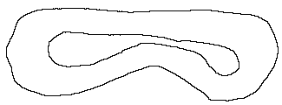
\includegraphics[interpolate=true,width=2.820000in,height=1.050000in]{contents/chapt5/figs/reward/path_collision_penalty-img0.png}}%
\end{pgfscope}%
\begin{pgfscope}%
\pgfpathrectangle{\pgfqpoint{0.180000in}{0.729385in}}{\pgfqpoint{2.820000in}{1.041231in}}%
\pgfusepath{clip}%
\pgfsetbuttcap%
\pgfsetroundjoin%
\pgfsetlinewidth{1.505625pt}%
\definecolor{currentstroke}{rgb}{0.501961,0.501961,0.501961}%
\pgfsetstrokecolor{currentstroke}%
\pgfsetdash{{5.550000pt}{2.400000pt}}{0.000000pt}%
\pgfpathmoveto{\pgfqpoint{1.741088in}{1.226736in}}%
\pgfpathlineto{\pgfqpoint{1.825202in}{1.205436in}}%
\pgfpathlineto{\pgfqpoint{1.892955in}{1.190069in}}%
\pgfpathlineto{\pgfqpoint{1.926172in}{1.180411in}}%
\pgfpathlineto{\pgfqpoint{1.975020in}{1.162462in}}%
\pgfpathlineto{\pgfqpoint{2.023590in}{1.142544in}}%
\pgfpathlineto{\pgfqpoint{2.054496in}{1.126725in}}%
\pgfpathlineto{\pgfqpoint{2.068883in}{1.117250in}}%
\pgfpathlineto{\pgfqpoint{2.095299in}{1.094914in}}%
\pgfpathlineto{\pgfqpoint{2.121014in}{1.071415in}}%
\pgfpathlineto{\pgfqpoint{2.134629in}{1.060626in}}%
\pgfpathlineto{\pgfqpoint{2.164225in}{1.042206in}}%
\pgfpathlineto{\pgfqpoint{2.194157in}{1.024485in}}%
\pgfpathlineto{\pgfqpoint{2.208044in}{1.014375in}}%
\pgfpathlineto{\pgfqpoint{2.220732in}{1.002820in}}%
\pgfpathlineto{\pgfqpoint{2.267859in}{0.951517in}}%
\pgfpathlineto{\pgfqpoint{2.281128in}{0.940164in}}%
\pgfpathlineto{\pgfqpoint{2.295393in}{0.930053in}}%
\pgfpathlineto{\pgfqpoint{2.310515in}{0.921239in}}%
\pgfpathlineto{\pgfqpoint{2.326352in}{0.913776in}}%
\pgfpathlineto{\pgfqpoint{2.342763in}{0.907719in}}%
\pgfpathlineto{\pgfqpoint{2.359611in}{0.903099in}}%
\pgfpathlineto{\pgfqpoint{2.376774in}{0.899863in}}%
\pgfpathlineto{\pgfqpoint{2.394131in}{0.897935in}}%
\pgfpathlineto{\pgfqpoint{2.411563in}{0.897239in}}%
\pgfpathlineto{\pgfqpoint{2.446204in}{0.899217in}}%
\pgfpathlineto{\pgfqpoint{2.480411in}{0.904673in}}%
\pgfpathlineto{\pgfqpoint{2.531651in}{0.915904in}}%
\pgfpathlineto{\pgfqpoint{2.565344in}{0.925242in}}%
\pgfpathlineto{\pgfqpoint{2.581544in}{0.931324in}}%
\pgfpathlineto{\pgfqpoint{2.597060in}{0.938793in}}%
\pgfpathlineto{\pgfqpoint{2.611735in}{0.947887in}}%
\pgfpathlineto{\pgfqpoint{2.625544in}{0.958454in}}%
\pgfpathlineto{\pgfqpoint{2.638495in}{0.970243in}}%
\pgfpathlineto{\pgfqpoint{2.661861in}{0.996497in}}%
\pgfpathlineto{\pgfqpoint{2.682043in}{1.024900in}}%
\pgfpathlineto{\pgfqpoint{2.699827in}{1.054676in}}%
\pgfpathlineto{\pgfqpoint{2.723717in}{1.100906in}}%
\pgfpathlineto{\pgfqpoint{2.737278in}{1.132885in}}%
\pgfpathlineto{\pgfqpoint{2.747746in}{1.166234in}}%
\pgfpathlineto{\pgfqpoint{2.751452in}{1.183382in}}%
\pgfpathlineto{\pgfqpoint{2.753912in}{1.200699in}}%
\pgfpathlineto{\pgfqpoint{2.754956in}{1.218072in}}%
\pgfpathlineto{\pgfqpoint{2.754411in}{1.235384in}}%
\pgfpathlineto{\pgfqpoint{2.752173in}{1.252535in}}%
\pgfpathlineto{\pgfqpoint{2.748411in}{1.269479in}}%
\pgfpathlineto{\pgfqpoint{2.737259in}{1.302617in}}%
\pgfpathlineto{\pgfqpoint{2.722781in}{1.334532in}}%
\pgfpathlineto{\pgfqpoint{2.705392in}{1.364665in}}%
\pgfpathlineto{\pgfqpoint{2.695296in}{1.378798in}}%
\pgfpathlineto{\pgfqpoint{2.684090in}{1.392163in}}%
\pgfpathlineto{\pgfqpoint{2.671684in}{1.404630in}}%
\pgfpathlineto{\pgfqpoint{2.658165in}{1.415976in}}%
\pgfpathlineto{\pgfqpoint{2.643665in}{1.425953in}}%
\pgfpathlineto{\pgfqpoint{2.628314in}{1.434315in}}%
\pgfpathlineto{\pgfqpoint{2.612244in}{1.440816in}}%
\pgfpathlineto{\pgfqpoint{2.595595in}{1.445366in}}%
\pgfpathlineto{\pgfqpoint{2.561291in}{1.450947in}}%
\pgfpathlineto{\pgfqpoint{2.526906in}{1.456511in}}%
\pgfpathlineto{\pgfqpoint{2.493537in}{1.466054in}}%
\pgfpathlineto{\pgfqpoint{2.443952in}{1.481956in}}%
\pgfpathlineto{\pgfqpoint{2.409984in}{1.488707in}}%
\pgfpathlineto{\pgfqpoint{2.358142in}{1.494821in}}%
\pgfpathlineto{\pgfqpoint{2.289304in}{1.503658in}}%
\pgfpathlineto{\pgfqpoint{2.220499in}{1.513871in}}%
\pgfpathlineto{\pgfqpoint{2.185942in}{1.516285in}}%
\pgfpathlineto{\pgfqpoint{2.151262in}{1.515154in}}%
\pgfpathlineto{\pgfqpoint{2.116551in}{1.513356in}}%
\pgfpathlineto{\pgfqpoint{2.081918in}{1.514585in}}%
\pgfpathlineto{\pgfqpoint{2.030066in}{1.520036in}}%
\pgfpathlineto{\pgfqpoint{2.012747in}{1.520582in}}%
\pgfpathlineto{\pgfqpoint{1.978025in}{1.518037in}}%
\pgfpathlineto{\pgfqpoint{1.943381in}{1.514867in}}%
\pgfpathlineto{\pgfqpoint{1.926167in}{1.514847in}}%
\pgfpathlineto{\pgfqpoint{1.909055in}{1.516602in}}%
\pgfpathlineto{\pgfqpoint{1.874988in}{1.523499in}}%
\pgfpathlineto{\pgfqpoint{1.840830in}{1.530542in}}%
\pgfpathlineto{\pgfqpoint{1.806307in}{1.533705in}}%
\pgfpathlineto{\pgfqpoint{1.771529in}{1.533836in}}%
\pgfpathlineto{\pgfqpoint{1.701944in}{1.532871in}}%
\pgfpathlineto{\pgfqpoint{1.667350in}{1.534846in}}%
\pgfpathlineto{\pgfqpoint{1.615765in}{1.542196in}}%
\pgfpathlineto{\pgfqpoint{1.581339in}{1.546290in}}%
\pgfpathlineto{\pgfqpoint{1.546712in}{1.547029in}}%
\pgfpathlineto{\pgfqpoint{1.407860in}{1.541986in}}%
\pgfpathlineto{\pgfqpoint{1.338516in}{1.537840in}}%
\pgfpathlineto{\pgfqpoint{1.303891in}{1.538269in}}%
\pgfpathlineto{\pgfqpoint{1.182509in}{1.545189in}}%
\pgfpathlineto{\pgfqpoint{1.147955in}{1.547721in}}%
\pgfpathlineto{\pgfqpoint{1.113707in}{1.553234in}}%
\pgfpathlineto{\pgfqpoint{1.062370in}{1.562003in}}%
\pgfpathlineto{\pgfqpoint{1.027787in}{1.564368in}}%
\pgfpathlineto{\pgfqpoint{0.993008in}{1.564130in}}%
\pgfpathlineto{\pgfqpoint{0.923547in}{1.561591in}}%
\pgfpathlineto{\pgfqpoint{0.888843in}{1.563437in}}%
\pgfpathlineto{\pgfqpoint{0.819662in}{1.573569in}}%
\pgfpathlineto{\pgfqpoint{0.802654in}{1.573458in}}%
\pgfpathlineto{\pgfqpoint{0.785839in}{1.570959in}}%
\pgfpathlineto{\pgfqpoint{0.769183in}{1.566498in}}%
\pgfpathlineto{\pgfqpoint{0.736161in}{1.554357in}}%
\pgfpathlineto{\pgfqpoint{0.703217in}{1.542223in}}%
\pgfpathlineto{\pgfqpoint{0.620726in}{1.515255in}}%
\pgfpathlineto{\pgfqpoint{0.588768in}{1.501033in}}%
\pgfpathlineto{\pgfqpoint{0.573703in}{1.492380in}}%
\pgfpathlineto{\pgfqpoint{0.559542in}{1.482448in}}%
\pgfpathlineto{\pgfqpoint{0.546460in}{1.471117in}}%
\pgfpathlineto{\pgfqpoint{0.534434in}{1.458552in}}%
\pgfpathlineto{\pgfqpoint{0.523397in}{1.444984in}}%
\pgfpathlineto{\pgfqpoint{0.504013in}{1.415774in}}%
\pgfpathlineto{\pgfqpoint{0.487828in}{1.385017in}}%
\pgfpathlineto{\pgfqpoint{0.474654in}{1.352912in}}%
\pgfpathlineto{\pgfqpoint{0.464416in}{1.319353in}}%
\pgfpathlineto{\pgfqpoint{0.460642in}{1.302139in}}%
\pgfpathlineto{\pgfqpoint{0.458094in}{1.284804in}}%
\pgfpathlineto{\pgfqpoint{0.457032in}{1.267481in}}%
\pgfpathlineto{\pgfqpoint{0.457714in}{1.250302in}}%
\pgfpathlineto{\pgfqpoint{0.460283in}{1.233366in}}%
\pgfpathlineto{\pgfqpoint{0.464415in}{1.216635in}}%
\pgfpathlineto{\pgfqpoint{0.475606in}{1.183494in}}%
\pgfpathlineto{\pgfqpoint{0.501047in}{1.117897in}}%
\pgfpathlineto{\pgfqpoint{0.508839in}{1.102529in}}%
\pgfpathlineto{\pgfqpoint{0.517948in}{1.088064in}}%
\pgfpathlineto{\pgfqpoint{0.528643in}{1.074688in}}%
\pgfpathlineto{\pgfqpoint{0.540753in}{1.062346in}}%
\pgfpathlineto{\pgfqpoint{0.553995in}{1.050921in}}%
\pgfpathlineto{\pgfqpoint{0.582749in}{1.030361in}}%
\pgfpathlineto{\pgfqpoint{0.613051in}{1.012462in}}%
\pgfpathlineto{\pgfqpoint{0.628683in}{1.004798in}}%
\pgfpathlineto{\pgfqpoint{0.644664in}{0.998219in}}%
\pgfpathlineto{\pgfqpoint{0.661014in}{0.992898in}}%
\pgfpathlineto{\pgfqpoint{0.694749in}{0.985912in}}%
\pgfpathlineto{\pgfqpoint{0.763852in}{0.975465in}}%
\pgfpathlineto{\pgfqpoint{0.798176in}{0.969015in}}%
\pgfpathlineto{\pgfqpoint{0.815293in}{0.966731in}}%
\pgfpathlineto{\pgfqpoint{0.832410in}{0.965751in}}%
\pgfpathlineto{\pgfqpoint{0.849546in}{0.966414in}}%
\pgfpathlineto{\pgfqpoint{0.883906in}{0.971175in}}%
\pgfpathlineto{\pgfqpoint{0.935740in}{0.979578in}}%
\pgfpathlineto{\pgfqpoint{0.987355in}{0.986519in}}%
\pgfpathlineto{\pgfqpoint{1.004231in}{0.990060in}}%
\pgfpathlineto{\pgfqpoint{1.037357in}{1.000102in}}%
\pgfpathlineto{\pgfqpoint{1.070392in}{1.011021in}}%
\pgfpathlineto{\pgfqpoint{1.087186in}{1.015505in}}%
\pgfpathlineto{\pgfqpoint{1.121543in}{1.021445in}}%
\pgfpathlineto{\pgfqpoint{1.155847in}{1.027002in}}%
\pgfpathlineto{\pgfqpoint{1.172524in}{1.031200in}}%
\pgfpathlineto{\pgfqpoint{1.188692in}{1.037005in}}%
\pgfpathlineto{\pgfqpoint{1.219829in}{1.052339in}}%
\pgfpathlineto{\pgfqpoint{1.295888in}{1.095141in}}%
\pgfpathlineto{\pgfqpoint{1.327143in}{1.109982in}}%
\pgfpathlineto{\pgfqpoint{1.359275in}{1.122977in}}%
\pgfpathlineto{\pgfqpoint{1.472845in}{1.166160in}}%
\pgfpathlineto{\pgfqpoint{1.568830in}{1.206599in}}%
\pgfpathlineto{\pgfqpoint{1.602059in}{1.215365in}}%
\pgfpathlineto{\pgfqpoint{1.636118in}{1.220971in}}%
\pgfpathlineto{\pgfqpoint{1.670799in}{1.224209in}}%
\pgfpathlineto{\pgfqpoint{1.723533in}{1.226352in}}%
\pgfpathlineto{\pgfqpoint{1.723533in}{1.226352in}}%
\pgfusepath{stroke}%
\end{pgfscope}%
\begin{pgfscope}%
\pgfpathrectangle{\pgfqpoint{0.180000in}{0.729385in}}{\pgfqpoint{2.820000in}{1.041231in}}%
\pgfusepath{clip}%
\pgfsetrectcap%
\pgfsetroundjoin%
\pgfsetlinewidth{1.505625pt}%
\definecolor{currentstroke}{rgb}{0.121569,0.466667,0.705882}%
\pgfsetstrokecolor{currentstroke}%
\pgfsetdash{}{0pt}%
\pgfpathmoveto{\pgfqpoint{1.915385in}{1.510308in}}%
\pgfpathlineto{\pgfqpoint{1.779910in}{1.511318in}}%
\pgfpathlineto{\pgfqpoint{1.683236in}{1.513813in}}%
\pgfpathlineto{\pgfqpoint{1.612670in}{1.517996in}}%
\pgfpathlineto{\pgfqpoint{1.542308in}{1.524814in}}%
\pgfpathlineto{\pgfqpoint{1.296348in}{1.551487in}}%
\pgfpathlineto{\pgfqpoint{1.234575in}{1.554661in}}%
\pgfpathlineto{\pgfqpoint{1.004979in}{1.562567in}}%
\pgfpathlineto{\pgfqpoint{0.907884in}{1.567063in}}%
\pgfpathlineto{\pgfqpoint{0.854869in}{1.567271in}}%
\pgfpathlineto{\pgfqpoint{0.819583in}{1.565300in}}%
\pgfpathlineto{\pgfqpoint{0.793278in}{1.562043in}}%
\pgfpathlineto{\pgfqpoint{0.767261in}{1.556978in}}%
\pgfpathlineto{\pgfqpoint{0.741741in}{1.549828in}}%
\pgfpathlineto{\pgfqpoint{0.716973in}{1.540401in}}%
\pgfpathlineto{\pgfqpoint{0.693296in}{1.528503in}}%
\pgfpathlineto{\pgfqpoint{0.671113in}{1.514011in}}%
\pgfpathlineto{\pgfqpoint{0.650810in}{1.496988in}}%
\pgfpathlineto{\pgfqpoint{0.638510in}{1.484302in}}%
\pgfpathlineto{\pgfqpoint{0.627335in}{1.470616in}}%
\pgfpathlineto{\pgfqpoint{0.617391in}{1.456011in}}%
\pgfpathlineto{\pgfqpoint{0.608776in}{1.440584in}}%
\pgfpathlineto{\pgfqpoint{0.601577in}{1.424448in}}%
\pgfpathlineto{\pgfqpoint{0.595866in}{1.407728in}}%
\pgfpathlineto{\pgfqpoint{0.591674in}{1.390563in}}%
\pgfpathlineto{\pgfqpoint{0.588099in}{1.364310in}}%
\pgfpathlineto{\pgfqpoint{0.587507in}{1.337817in}}%
\pgfpathlineto{\pgfqpoint{0.589530in}{1.311393in}}%
\pgfpathlineto{\pgfqpoint{0.593903in}{1.285252in}}%
\pgfpathlineto{\pgfqpoint{0.600287in}{1.259527in}}%
\pgfpathlineto{\pgfqpoint{0.608400in}{1.234293in}}%
\pgfpathlineto{\pgfqpoint{0.621641in}{1.201529in}}%
\pgfpathlineto{\pgfqpoint{0.637348in}{1.169872in}}%
\pgfpathlineto{\pgfqpoint{0.655327in}{1.139448in}}%
\pgfpathlineto{\pgfqpoint{0.675457in}{1.110401in}}%
\pgfpathlineto{\pgfqpoint{0.697631in}{1.082883in}}%
\pgfpathlineto{\pgfqpoint{0.715597in}{1.063395in}}%
\pgfpathlineto{\pgfqpoint{0.734882in}{1.045213in}}%
\pgfpathlineto{\pgfqpoint{0.755627in}{1.028720in}}%
\pgfpathlineto{\pgfqpoint{0.777825in}{1.014244in}}%
\pgfpathlineto{\pgfqpoint{0.801395in}{1.002134in}}%
\pgfpathlineto{\pgfqpoint{0.826184in}{0.992778in}}%
\pgfpathlineto{\pgfqpoint{0.851922in}{0.986489in}}%
\pgfpathlineto{\pgfqpoint{0.878232in}{0.983347in}}%
\pgfpathlineto{\pgfqpoint{0.904730in}{0.983152in}}%
\pgfpathlineto{\pgfqpoint{0.931121in}{0.985578in}}%
\pgfpathlineto{\pgfqpoint{0.957189in}{0.990360in}}%
\pgfpathlineto{\pgfqpoint{0.982791in}{0.997216in}}%
\pgfpathlineto{\pgfqpoint{1.007857in}{1.005835in}}%
\pgfpathlineto{\pgfqpoint{1.040212in}{1.019508in}}%
\pgfpathlineto{\pgfqpoint{1.086910in}{1.042496in}}%
\pgfpathlineto{\pgfqpoint{1.148061in}{1.072676in}}%
\pgfpathlineto{\pgfqpoint{1.179234in}{1.085949in}}%
\pgfpathlineto{\pgfqpoint{1.220181in}{1.100709in}}%
\pgfpathlineto{\pgfqpoint{1.270142in}{1.116266in}}%
\pgfpathlineto{\pgfqpoint{1.345812in}{1.137136in}}%
\pgfpathlineto{\pgfqpoint{1.430461in}{1.158139in}}%
\pgfpathlineto{\pgfqpoint{1.498720in}{1.172588in}}%
\pgfpathlineto{\pgfqpoint{1.541713in}{1.179871in}}%
\pgfpathlineto{\pgfqpoint{1.585027in}{1.184890in}}%
\pgfpathlineto{\pgfqpoint{1.619851in}{1.186921in}}%
\pgfpathlineto{\pgfqpoint{1.654733in}{1.186889in}}%
\pgfpathlineto{\pgfqpoint{1.689542in}{1.184633in}}%
\pgfpathlineto{\pgfqpoint{1.724162in}{1.180355in}}%
\pgfpathlineto{\pgfqpoint{1.758490in}{1.174154in}}%
\pgfpathlineto{\pgfqpoint{1.800880in}{1.163945in}}%
\pgfpathlineto{\pgfqpoint{1.842602in}{1.151271in}}%
\pgfpathlineto{\pgfqpoint{1.883577in}{1.136357in}}%
\pgfpathlineto{\pgfqpoint{1.923716in}{1.119321in}}%
\pgfpathlineto{\pgfqpoint{1.962937in}{1.100265in}}%
\pgfpathlineto{\pgfqpoint{2.001141in}{1.079245in}}%
\pgfpathlineto{\pgfqpoint{2.045789in}{1.051954in}}%
\pgfpathlineto{\pgfqpoint{2.111382in}{1.008837in}}%
\pgfpathlineto{\pgfqpoint{2.198731in}{0.951191in}}%
\pgfpathlineto{\pgfqpoint{2.228935in}{0.933740in}}%
\pgfpathlineto{\pgfqpoint{2.260187in}{0.918250in}}%
\pgfpathlineto{\pgfqpoint{2.284384in}{0.908303in}}%
\pgfpathlineto{\pgfqpoint{2.309220in}{0.900085in}}%
\pgfpathlineto{\pgfqpoint{2.334647in}{0.893946in}}%
\pgfpathlineto{\pgfqpoint{2.360527in}{0.890143in}}%
\pgfpathlineto{\pgfqpoint{2.386650in}{0.888838in}}%
\pgfpathlineto{\pgfqpoint{2.412771in}{0.890192in}}%
\pgfpathlineto{\pgfqpoint{2.438603in}{0.894284in}}%
\pgfpathlineto{\pgfqpoint{2.463838in}{0.901158in}}%
\pgfpathlineto{\pgfqpoint{2.488150in}{0.910796in}}%
\pgfpathlineto{\pgfqpoint{2.511128in}{0.923281in}}%
\pgfpathlineto{\pgfqpoint{2.532409in}{0.938479in}}%
\pgfpathlineto{\pgfqpoint{2.551605in}{0.956237in}}%
\pgfpathlineto{\pgfqpoint{2.563063in}{0.969384in}}%
\pgfpathlineto{\pgfqpoint{2.573326in}{0.983484in}}%
\pgfpathlineto{\pgfqpoint{2.582299in}{0.998437in}}%
\pgfpathlineto{\pgfqpoint{2.589899in}{1.014133in}}%
\pgfpathlineto{\pgfqpoint{2.596053in}{1.030451in}}%
\pgfpathlineto{\pgfqpoint{2.600729in}{1.047252in}}%
\pgfpathlineto{\pgfqpoint{2.605102in}{1.073035in}}%
\pgfpathlineto{\pgfqpoint{2.606571in}{1.099149in}}%
\pgfpathlineto{\pgfqpoint{2.605494in}{1.125284in}}%
\pgfpathlineto{\pgfqpoint{2.602124in}{1.151226in}}%
\pgfpathlineto{\pgfqpoint{2.596786in}{1.176836in}}%
\pgfpathlineto{\pgfqpoint{2.587051in}{1.210328in}}%
\pgfpathlineto{\pgfqpoint{2.574497in}{1.242869in}}%
\pgfpathlineto{\pgfqpoint{2.559345in}{1.274284in}}%
\pgfpathlineto{\pgfqpoint{2.541687in}{1.304362in}}%
\pgfpathlineto{\pgfqpoint{2.521585in}{1.332865in}}%
\pgfpathlineto{\pgfqpoint{2.504955in}{1.353061in}}%
\pgfpathlineto{\pgfqpoint{2.486982in}{1.372071in}}%
\pgfpathlineto{\pgfqpoint{2.467731in}{1.389784in}}%
\pgfpathlineto{\pgfqpoint{2.447257in}{1.406069in}}%
\pgfpathlineto{\pgfqpoint{2.425649in}{1.420816in}}%
\pgfpathlineto{\pgfqpoint{2.402994in}{1.433897in}}%
\pgfpathlineto{\pgfqpoint{2.379415in}{1.445227in}}%
\pgfpathlineto{\pgfqpoint{2.355043in}{1.454734in}}%
\pgfpathlineto{\pgfqpoint{2.321687in}{1.464931in}}%
\pgfpathlineto{\pgfqpoint{2.287684in}{1.472709in}}%
\pgfpathlineto{\pgfqpoint{2.253270in}{1.478417in}}%
\pgfpathlineto{\pgfqpoint{2.209935in}{1.483252in}}%
\pgfpathlineto{\pgfqpoint{2.157714in}{1.486614in}}%
\pgfpathlineto{\pgfqpoint{2.070548in}{1.489591in}}%
\pgfpathlineto{\pgfqpoint{1.922367in}{1.494702in}}%
\pgfpathlineto{\pgfqpoint{1.896234in}{1.496009in}}%
\pgfpathlineto{\pgfqpoint{1.896234in}{1.496009in}}%
\pgfusepath{stroke}%
\end{pgfscope}%
\begin{pgfscope}%
\pgfpathrectangle{\pgfqpoint{0.180000in}{0.729385in}}{\pgfqpoint{2.820000in}{1.041231in}}%
\pgfusepath{clip}%
\pgfsetrectcap%
\pgfsetroundjoin%
\pgfsetlinewidth{1.505625pt}%
\definecolor{currentstroke}{rgb}{1.000000,0.498039,0.054902}%
\pgfsetstrokecolor{currentstroke}%
\pgfsetdash{}{0pt}%
\pgfpathmoveto{\pgfqpoint{1.915385in}{1.510308in}}%
\pgfpathlineto{\pgfqpoint{1.842619in}{1.511410in}}%
\pgfpathlineto{\pgfqpoint{1.779172in}{1.514666in}}%
\pgfpathlineto{\pgfqpoint{1.685769in}{1.522011in}}%
\pgfpathlineto{\pgfqpoint{1.517654in}{1.536185in}}%
\pgfpathlineto{\pgfqpoint{1.456438in}{1.538861in}}%
\pgfpathlineto{\pgfqpoint{1.360156in}{1.540335in}}%
\pgfpathlineto{\pgfqpoint{1.088790in}{1.541428in}}%
\pgfpathlineto{\pgfqpoint{1.018794in}{1.539241in}}%
\pgfpathlineto{\pgfqpoint{0.957650in}{1.535240in}}%
\pgfpathlineto{\pgfqpoint{0.896703in}{1.528920in}}%
\pgfpathlineto{\pgfqpoint{0.836065in}{1.520111in}}%
\pgfpathlineto{\pgfqpoint{0.784421in}{1.510553in}}%
\pgfpathlineto{\pgfqpoint{0.741712in}{1.500989in}}%
\pgfpathlineto{\pgfqpoint{0.708028in}{1.491443in}}%
\pgfpathlineto{\pgfqpoint{0.683314in}{1.482573in}}%
\pgfpathlineto{\pgfqpoint{0.659316in}{1.471922in}}%
\pgfpathlineto{\pgfqpoint{0.636310in}{1.459272in}}%
\pgfpathlineto{\pgfqpoint{0.614645in}{1.444446in}}%
\pgfpathlineto{\pgfqpoint{0.594694in}{1.427389in}}%
\pgfpathlineto{\pgfqpoint{0.576960in}{1.408039in}}%
\pgfpathlineto{\pgfqpoint{0.566563in}{1.393958in}}%
\pgfpathlineto{\pgfqpoint{0.557443in}{1.379018in}}%
\pgfpathlineto{\pgfqpoint{0.549710in}{1.363315in}}%
\pgfpathlineto{\pgfqpoint{0.543464in}{1.346965in}}%
\pgfpathlineto{\pgfqpoint{0.538789in}{1.330098in}}%
\pgfpathlineto{\pgfqpoint{0.535752in}{1.312860in}}%
\pgfpathlineto{\pgfqpoint{0.534401in}{1.295410in}}%
\pgfpathlineto{\pgfqpoint{0.534737in}{1.277910in}}%
\pgfpathlineto{\pgfqpoint{0.536665in}{1.260513in}}%
\pgfpathlineto{\pgfqpoint{0.542294in}{1.234876in}}%
\pgfpathlineto{\pgfqpoint{0.550846in}{1.210058in}}%
\pgfpathlineto{\pgfqpoint{0.562028in}{1.186307in}}%
\pgfpathlineto{\pgfqpoint{0.575475in}{1.163758in}}%
\pgfpathlineto{\pgfqpoint{0.590878in}{1.142496in}}%
\pgfpathlineto{\pgfqpoint{0.607961in}{1.122557in}}%
\pgfpathlineto{\pgfqpoint{0.626448in}{1.103911in}}%
\pgfpathlineto{\pgfqpoint{0.646168in}{1.086574in}}%
\pgfpathlineto{\pgfqpoint{0.674110in}{1.065485in}}%
\pgfpathlineto{\pgfqpoint{0.703662in}{1.046719in}}%
\pgfpathlineto{\pgfqpoint{0.734574in}{1.030287in}}%
\pgfpathlineto{\pgfqpoint{0.766653in}{1.016270in}}%
\pgfpathlineto{\pgfqpoint{0.799748in}{1.004858in}}%
\pgfpathlineto{\pgfqpoint{0.833659in}{0.996167in}}%
\pgfpathlineto{\pgfqpoint{0.868176in}{0.990333in}}%
\pgfpathlineto{\pgfqpoint{0.894321in}{0.987903in}}%
\pgfpathlineto{\pgfqpoint{0.920569in}{0.987165in}}%
\pgfpathlineto{\pgfqpoint{0.955548in}{0.988594in}}%
\pgfpathlineto{\pgfqpoint{0.990324in}{0.992628in}}%
\pgfpathlineto{\pgfqpoint{1.024733in}{0.999089in}}%
\pgfpathlineto{\pgfqpoint{1.058648in}{1.007779in}}%
\pgfpathlineto{\pgfqpoint{1.091964in}{1.018543in}}%
\pgfpathlineto{\pgfqpoint{1.132824in}{1.034224in}}%
\pgfpathlineto{\pgfqpoint{1.181032in}{1.055068in}}%
\pgfpathlineto{\pgfqpoint{1.372787in}{1.140855in}}%
\pgfpathlineto{\pgfqpoint{1.430080in}{1.162583in}}%
\pgfpathlineto{\pgfqpoint{1.488197in}{1.181995in}}%
\pgfpathlineto{\pgfqpoint{1.538617in}{1.196705in}}%
\pgfpathlineto{\pgfqpoint{1.589552in}{1.209511in}}%
\pgfpathlineto{\pgfqpoint{1.632497in}{1.217944in}}%
\pgfpathlineto{\pgfqpoint{1.667164in}{1.222846in}}%
\pgfpathlineto{\pgfqpoint{1.702051in}{1.225795in}}%
\pgfpathlineto{\pgfqpoint{1.737053in}{1.226561in}}%
\pgfpathlineto{\pgfqpoint{1.771945in}{1.225156in}}%
\pgfpathlineto{\pgfqpoint{1.806556in}{1.221764in}}%
\pgfpathlineto{\pgfqpoint{1.840781in}{1.216470in}}%
\pgfpathlineto{\pgfqpoint{1.882904in}{1.207421in}}%
\pgfpathlineto{\pgfqpoint{1.924108in}{1.195936in}}%
\pgfpathlineto{\pgfqpoint{1.963704in}{1.182138in}}%
\pgfpathlineto{\pgfqpoint{1.994025in}{1.169423in}}%
\pgfpathlineto{\pgfqpoint{2.023002in}{1.155185in}}%
\pgfpathlineto{\pgfqpoint{2.050505in}{1.139439in}}%
\pgfpathlineto{\pgfqpoint{2.076385in}{1.122313in}}%
\pgfpathlineto{\pgfqpoint{2.100558in}{1.104100in}}%
\pgfpathlineto{\pgfqpoint{2.128336in}{1.080039in}}%
\pgfpathlineto{\pgfqpoint{2.153460in}{1.054887in}}%
\pgfpathlineto{\pgfqpoint{2.176196in}{1.028787in}}%
\pgfpathlineto{\pgfqpoint{2.231532in}{0.962353in}}%
\pgfpathlineto{\pgfqpoint{2.252696in}{0.940970in}}%
\pgfpathlineto{\pgfqpoint{2.275892in}{0.920735in}}%
\pgfpathlineto{\pgfqpoint{2.294960in}{0.906623in}}%
\pgfpathlineto{\pgfqpoint{2.315550in}{0.893754in}}%
\pgfpathlineto{\pgfqpoint{2.337625in}{0.882367in}}%
\pgfpathlineto{\pgfqpoint{2.361111in}{0.872702in}}%
\pgfpathlineto{\pgfqpoint{2.385900in}{0.865010in}}%
\pgfpathlineto{\pgfqpoint{2.411479in}{0.859618in}}%
\pgfpathlineto{\pgfqpoint{2.437466in}{0.856792in}}%
\pgfpathlineto{\pgfqpoint{2.463604in}{0.856701in}}%
\pgfpathlineto{\pgfqpoint{2.489587in}{0.859531in}}%
\pgfpathlineto{\pgfqpoint{2.515056in}{0.865394in}}%
\pgfpathlineto{\pgfqpoint{2.539635in}{0.874278in}}%
\pgfpathlineto{\pgfqpoint{2.562934in}{0.886119in}}%
\pgfpathlineto{\pgfqpoint{2.584581in}{0.900747in}}%
\pgfpathlineto{\pgfqpoint{2.604299in}{0.917788in}}%
\pgfpathlineto{\pgfqpoint{2.622049in}{0.936769in}}%
\pgfpathlineto{\pgfqpoint{2.637800in}{0.957344in}}%
\pgfpathlineto{\pgfqpoint{2.651558in}{0.979213in}}%
\pgfpathlineto{\pgfqpoint{2.663392in}{1.002097in}}%
\pgfpathlineto{\pgfqpoint{2.673417in}{1.025747in}}%
\pgfpathlineto{\pgfqpoint{2.681721in}{1.049999in}}%
\pgfpathlineto{\pgfqpoint{2.688254in}{1.074781in}}%
\pgfpathlineto{\pgfqpoint{2.692989in}{1.099962in}}%
\pgfpathlineto{\pgfqpoint{2.695931in}{1.125408in}}%
\pgfpathlineto{\pgfqpoint{2.697024in}{1.150995in}}%
\pgfpathlineto{\pgfqpoint{2.696243in}{1.176587in}}%
\pgfpathlineto{\pgfqpoint{2.693549in}{1.202042in}}%
\pgfpathlineto{\pgfqpoint{2.688880in}{1.227481in}}%
\pgfpathlineto{\pgfqpoint{2.682057in}{1.252704in}}%
\pgfpathlineto{\pgfqpoint{2.673109in}{1.277254in}}%
\pgfpathlineto{\pgfqpoint{2.662024in}{1.300916in}}%
\pgfpathlineto{\pgfqpoint{2.648743in}{1.323416in}}%
\pgfpathlineto{\pgfqpoint{2.633280in}{1.344476in}}%
\pgfpathlineto{\pgfqpoint{2.615693in}{1.363796in}}%
\pgfpathlineto{\pgfqpoint{2.596183in}{1.381174in}}%
\pgfpathlineto{\pgfqpoint{2.575120in}{1.396637in}}%
\pgfpathlineto{\pgfqpoint{2.552780in}{1.410190in}}%
\pgfpathlineto{\pgfqpoint{2.529400in}{1.421861in}}%
\pgfpathlineto{\pgfqpoint{2.505199in}{1.431721in}}%
\pgfpathlineto{\pgfqpoint{2.480374in}{1.439883in}}%
\pgfpathlineto{\pgfqpoint{2.446572in}{1.448334in}}%
\pgfpathlineto{\pgfqpoint{2.403718in}{1.456122in}}%
\pgfpathlineto{\pgfqpoint{2.351878in}{1.462823in}}%
\pgfpathlineto{\pgfqpoint{2.239170in}{1.473994in}}%
\pgfpathlineto{\pgfqpoint{2.126572in}{1.486207in}}%
\pgfpathlineto{\pgfqpoint{1.962208in}{1.505859in}}%
\pgfpathlineto{\pgfqpoint{1.962208in}{1.505859in}}%
\pgfusepath{stroke}%
\end{pgfscope}%
\begin{pgfscope}%
\pgfpathrectangle{\pgfqpoint{0.180000in}{0.729385in}}{\pgfqpoint{2.820000in}{1.041231in}}%
\pgfusepath{clip}%
\pgfsetbuttcap%
\pgfsetroundjoin%
\pgfsetlinewidth{1.505625pt}%
\definecolor{currentstroke}{rgb}{1.000000,0.000000,0.000000}%
\pgfsetstrokecolor{currentstroke}%
\pgfsetdash{{1.500000pt}{2.475000pt}}{0.000000pt}%
\pgfpathmoveto{\pgfqpoint{1.909055in}{1.343063in}}%
\pgfpathlineto{\pgfqpoint{1.909055in}{1.690140in}}%
\pgfusepath{stroke}%
\end{pgfscope}%
\begin{pgfscope}%
\pgfsetbuttcap%
\pgfsetmiterjoin%
\definecolor{currentfill}{rgb}{1.000000,1.000000,1.000000}%
\pgfsetfillcolor{currentfill}%
\pgfsetlinewidth{1.003750pt}%
\definecolor{currentstroke}{rgb}{0.000000,0.000000,0.000000}%
\pgfsetstrokecolor{currentstroke}%
\pgfsetdash{}{0pt}%
\pgfpathmoveto{\pgfqpoint{1.700809in}{1.693610in}}%
\pgfpathlineto{\pgfqpoint{2.404139in}{1.693610in}}%
\pgfpathquadraticcurveto{\pgfqpoint{2.418022in}{1.693610in}}{\pgfqpoint{2.418022in}{1.707494in}}%
\pgfpathlineto{\pgfqpoint{2.418022in}{1.846327in}}%
\pgfpathquadraticcurveto{\pgfqpoint{2.418022in}{1.860210in}}{\pgfqpoint{2.404139in}{1.860210in}}%
\pgfpathlineto{\pgfqpoint{1.700809in}{1.860210in}}%
\pgfpathquadraticcurveto{\pgfqpoint{1.686925in}{1.860210in}}{\pgfqpoint{1.686925in}{1.846327in}}%
\pgfpathlineto{\pgfqpoint{1.686925in}{1.707494in}}%
\pgfpathquadraticcurveto{\pgfqpoint{1.686925in}{1.693610in}}{\pgfqpoint{1.700809in}{1.693610in}}%
\pgfpathlineto{\pgfqpoint{1.700809in}{1.693610in}}%
\pgfpathclose%
\pgfusepath{stroke,fill}%
\end{pgfscope}%
\begin{pgfscope}%
\definecolor{textcolor}{rgb}{0.000000,0.000000,0.000000}%
\pgfsetstrokecolor{textcolor}%
\pgfsetfillcolor{textcolor}%
\pgftext[x=1.700809in,y=1.742202in,left,base]{\color{textcolor}\rmfamily\fontsize{9.996000}{11.995200}\selectfont Start/finish}%
\end{pgfscope}%
\begin{pgfscope}%
\pgfsetbuttcap%
\pgfsetmiterjoin%
\definecolor{currentfill}{rgb}{1.000000,1.000000,1.000000}%
\pgfsetfillcolor{currentfill}%
\pgfsetfillopacity{0.800000}%
\pgfsetlinewidth{1.003750pt}%
\definecolor{currentstroke}{rgb}{0.800000,0.800000,0.800000}%
\pgfsetstrokecolor{currentstroke}%
\pgfsetstrokeopacity{0.800000}%
\pgfsetdash{}{0pt}%
\pgfpathmoveto{\pgfqpoint{3.207667in}{0.876500in}}%
\pgfpathlineto{\pgfqpoint{4.883333in}{0.876500in}}%
\pgfpathquadraticcurveto{\pgfqpoint{4.916667in}{0.876500in}}{\pgfqpoint{4.916667in}{0.909834in}}%
\pgfpathlineto{\pgfqpoint{4.916667in}{1.590166in}}%
\pgfpathquadraticcurveto{\pgfqpoint{4.916667in}{1.623500in}}{\pgfqpoint{4.883333in}{1.623500in}}%
\pgfpathlineto{\pgfqpoint{3.207667in}{1.623500in}}%
\pgfpathquadraticcurveto{\pgfqpoint{3.174333in}{1.623500in}}{\pgfqpoint{3.174333in}{1.590166in}}%
\pgfpathlineto{\pgfqpoint{3.174333in}{0.909834in}}%
\pgfpathquadraticcurveto{\pgfqpoint{3.174333in}{0.876500in}}{\pgfqpoint{3.207667in}{0.876500in}}%
\pgfpathlineto{\pgfqpoint{3.207667in}{0.876500in}}%
\pgfpathclose%
\pgfusepath{stroke,fill}%
\end{pgfscope}%
\begin{pgfscope}%
\pgfsetbuttcap%
\pgfsetroundjoin%
\pgfsetlinewidth{1.505625pt}%
\definecolor{currentstroke}{rgb}{0.501961,0.501961,0.501961}%
\pgfsetstrokecolor{currentstroke}%
\pgfsetdash{{5.550000pt}{2.400000pt}}{0.000000pt}%
\pgfpathmoveto{\pgfqpoint{3.241000in}{1.498500in}}%
\pgfpathlineto{\pgfqpoint{3.407667in}{1.498500in}}%
\pgfpathlineto{\pgfqpoint{3.574333in}{1.498500in}}%
\pgfusepath{stroke}%
\end{pgfscope}%
\begin{pgfscope}%
\definecolor{textcolor}{rgb}{0.000000,0.000000,0.000000}%
\pgfsetstrokecolor{textcolor}%
\pgfsetfillcolor{textcolor}%
\pgftext[x=3.707667in,y=1.440166in,left,base]{\color{textcolor}\rmfamily\fontsize{12.000000}{14.400000}\selectfont Track centerline}%
\end{pgfscope}%
\begin{pgfscope}%
\pgfsetrectcap%
\pgfsetroundjoin%
\pgfsetlinewidth{1.505625pt}%
\definecolor{currentstroke}{rgb}{0.121569,0.466667,0.705882}%
\pgfsetstrokecolor{currentstroke}%
\pgfsetdash{}{0pt}%
\pgfpathmoveto{\pgfqpoint{3.241000in}{1.266167in}}%
\pgfpathlineto{\pgfqpoint{3.407667in}{1.266167in}}%
\pgfpathlineto{\pgfqpoint{3.574333in}{1.266167in}}%
\pgfusepath{stroke}%
\end{pgfscope}%
\begin{pgfscope}%
\definecolor{textcolor}{rgb}{0.000000,0.000000,0.000000}%
\pgfsetstrokecolor{textcolor}%
\pgfsetfillcolor{textcolor}%
\pgftext[x=3.707667in,y=1.207833in,left,base]{\color{textcolor}\rmfamily\fontsize{12.000000}{14.400000}\selectfont \(\displaystyle r_{\mathrm{collision}}=-4\)}%
\end{pgfscope}%
\begin{pgfscope}%
\pgfsetrectcap%
\pgfsetroundjoin%
\pgfsetlinewidth{1.505625pt}%
\definecolor{currentstroke}{rgb}{1.000000,0.498039,0.054902}%
\pgfsetstrokecolor{currentstroke}%
\pgfsetdash{}{0pt}%
\pgfpathmoveto{\pgfqpoint{3.241000in}{1.033833in}}%
\pgfpathlineto{\pgfqpoint{3.407667in}{1.033833in}}%
\pgfpathlineto{\pgfqpoint{3.574333in}{1.033833in}}%
\pgfusepath{stroke}%
\end{pgfscope}%
\begin{pgfscope}%
\definecolor{textcolor}{rgb}{0.000000,0.000000,0.000000}%
\pgfsetstrokecolor{textcolor}%
\pgfsetfillcolor{textcolor}%
\pgftext[x=3.707667in,y=0.975500in,left,base]{\color{textcolor}\rmfamily\fontsize{12.000000}{14.400000}\selectfont \(\displaystyle r_{\mathrm{collision}}=-10\)}%
\end{pgfscope}%
\end{pgfpicture}%
\makeatother%
\endgroup%

    \caption[Paths taken by agents trained with different collision penalties]{The paths taken by agents trained with different penalties for colliding with the track boundary.}
    \label{fig:path_reward_collision}
\end{figure}


\section{Evaluation of an end-to-end agent}
The hyper-parameters that we selected throughout this chapter were used to train an end-to-end agent that was used as a baseline comparison to measure the performance of the partial end-to-end agents presented in Chapters \ref{chp:partial_end_to_end_autonomous_racing} and \ref{chp:racing}.
% The normal training and testing procedure from Section \ref{sec:train_and_test_procedures} was followed.
We now present the learning curves for training, tabulated test results, and a qualitative evaluation of this agent's performance during a single test lap.

The learning curves presented in Figure \ref{fig:end_to_end_learning} show that our end-to-end agent learns to maximise reward by minimising the failure rate (i.e., by avoiding track boundaries) and minimising lap time within about $2\cdot10^3$ episodes.
It completes training within $3\cdot10^3$ episodes.
Furthermore, the learning curves are steady and do not fluctuate around their final values.

\begin{figure}[htb!]
    \centering
    %% Creator: Matplotlib, PGF backend
%%
%% To include the figure in your LaTeX document, write
%%   \input{<filename>.pgf}
%%
%% Make sure the required packages are loaded in your preamble
%%   \usepackage{pgf}
%%
%% Also ensure that all the required font packages are loaded; for instance,
%% the lmodern package is sometimes necessary when using math font.
%%   \usepackage{lmodern}
%%
%% Figures using additional raster images can only be included by \input if
%% they are in the same directory as the main LaTeX file. For loading figures
%% from other directories you can use the `import` package
%%   \usepackage{import}
%%
%% and then include the figures with
%%   \import{<path to file>}{<filename>.pgf}
%%
%% Matplotlib used the following preamble
%%   \usepackage{fontspec}
%%
\begingroup%
\makeatletter%
\begin{pgfpicture}%
\pgfpathrectangle{\pgfpointorigin}{\pgfqpoint{5.500000in}{2.100000in}}%
\pgfusepath{use as bounding box, clip}%
\begin{pgfscope}%
\pgfsetbuttcap%
\pgfsetmiterjoin%
\definecolor{currentfill}{rgb}{1.000000,1.000000,1.000000}%
\pgfsetfillcolor{currentfill}%
\pgfsetlinewidth{0.000000pt}%
\definecolor{currentstroke}{rgb}{1.000000,1.000000,1.000000}%
\pgfsetstrokecolor{currentstroke}%
\pgfsetdash{}{0pt}%
\pgfpathmoveto{\pgfqpoint{0.000000in}{0.000000in}}%
\pgfpathlineto{\pgfqpoint{5.500000in}{0.000000in}}%
\pgfpathlineto{\pgfqpoint{5.500000in}{2.100000in}}%
\pgfpathlineto{\pgfqpoint{0.000000in}{2.100000in}}%
\pgfpathlineto{\pgfqpoint{0.000000in}{0.000000in}}%
\pgfpathclose%
\pgfusepath{fill}%
\end{pgfscope}%
\begin{pgfscope}%
\pgfsetbuttcap%
\pgfsetmiterjoin%
\definecolor{currentfill}{rgb}{1.000000,1.000000,1.000000}%
\pgfsetfillcolor{currentfill}%
\pgfsetlinewidth{0.000000pt}%
\definecolor{currentstroke}{rgb}{0.000000,0.000000,0.000000}%
\pgfsetstrokecolor{currentstroke}%
\pgfsetstrokeopacity{0.000000}%
\pgfsetdash{}{0pt}%
\pgfpathmoveto{\pgfqpoint{0.473611in}{0.604920in}}%
\pgfpathlineto{\pgfqpoint{1.700618in}{0.604920in}}%
\pgfpathlineto{\pgfqpoint{1.700618in}{1.711667in}}%
\pgfpathlineto{\pgfqpoint{0.473611in}{1.711667in}}%
\pgfpathlineto{\pgfqpoint{0.473611in}{0.604920in}}%
\pgfpathclose%
\pgfusepath{fill}%
\end{pgfscope}%
\begin{pgfscope}%
\pgfpathrectangle{\pgfqpoint{0.473611in}{0.604920in}}{\pgfqpoint{1.227007in}{1.106747in}}%
\pgfusepath{clip}%
\pgfsetbuttcap%
\pgfsetroundjoin%
\definecolor{currentfill}{rgb}{0.121569,0.466667,0.705882}%
\pgfsetfillcolor{currentfill}%
\pgfsetfillopacity{0.150000}%
\pgfsetlinewidth{0.000000pt}%
\definecolor{currentstroke}{rgb}{0.000000,0.000000,0.000000}%
\pgfsetstrokecolor{currentstroke}%
\pgfsetdash{}{0pt}%
\pgfpathmoveto{\pgfqpoint{0.473611in}{1.661360in}}%
\pgfpathlineto{\pgfqpoint{0.473611in}{1.661360in}}%
\pgfpathlineto{\pgfqpoint{0.514511in}{1.661360in}}%
\pgfpathlineto{\pgfqpoint{0.555412in}{1.720101in}}%
\pgfpathlineto{\pgfqpoint{0.596312in}{1.629232in}}%
\pgfpathlineto{\pgfqpoint{0.637212in}{1.569168in}}%
\pgfpathlineto{\pgfqpoint{0.678112in}{1.514454in}}%
\pgfpathlineto{\pgfqpoint{0.719013in}{1.273585in}}%
\pgfpathlineto{\pgfqpoint{0.759913in}{1.169808in}}%
\pgfpathlineto{\pgfqpoint{0.800813in}{1.107773in}}%
\pgfpathlineto{\pgfqpoint{0.841713in}{1.035604in}}%
\pgfpathlineto{\pgfqpoint{0.882613in}{0.984035in}}%
\pgfpathlineto{\pgfqpoint{0.923514in}{0.973455in}}%
\pgfpathlineto{\pgfqpoint{0.964414in}{0.957509in}}%
\pgfpathlineto{\pgfqpoint{1.005314in}{0.950994in}}%
\pgfpathlineto{\pgfqpoint{1.046214in}{0.961310in}}%
\pgfpathlineto{\pgfqpoint{1.087115in}{0.954962in}}%
\pgfpathlineto{\pgfqpoint{1.128015in}{0.943714in}}%
\pgfpathlineto{\pgfqpoint{1.168915in}{0.956469in}}%
\pgfpathlineto{\pgfqpoint{1.209815in}{0.960780in}}%
\pgfpathlineto{\pgfqpoint{1.250716in}{0.948498in}}%
\pgfpathlineto{\pgfqpoint{1.291616in}{0.950264in}}%
\pgfpathlineto{\pgfqpoint{1.332516in}{0.955284in}}%
\pgfpathlineto{\pgfqpoint{1.373416in}{0.938193in}}%
\pgfpathlineto{\pgfqpoint{1.414317in}{0.933840in}}%
\pgfpathlineto{\pgfqpoint{1.455217in}{0.937283in}}%
\pgfpathlineto{\pgfqpoint{1.496117in}{0.941249in}}%
\pgfpathlineto{\pgfqpoint{1.537017in}{0.954632in}}%
\pgfpathlineto{\pgfqpoint{1.577917in}{0.962161in}}%
\pgfpathlineto{\pgfqpoint{1.618818in}{0.959789in}}%
\pgfpathlineto{\pgfqpoint{1.659718in}{0.949896in}}%
\pgfpathlineto{\pgfqpoint{1.659718in}{0.589498in}}%
\pgfpathlineto{\pgfqpoint{1.659718in}{0.589498in}}%
\pgfpathlineto{\pgfqpoint{1.618818in}{0.583622in}}%
\pgfpathlineto{\pgfqpoint{1.577917in}{0.581249in}}%
\pgfpathlineto{\pgfqpoint{1.537017in}{0.580745in}}%
\pgfpathlineto{\pgfqpoint{1.496117in}{0.579402in}}%
\pgfpathlineto{\pgfqpoint{1.455217in}{0.579351in}}%
\pgfpathlineto{\pgfqpoint{1.414317in}{0.581455in}}%
\pgfpathlineto{\pgfqpoint{1.373416in}{0.579780in}}%
\pgfpathlineto{\pgfqpoint{1.332516in}{0.577415in}}%
\pgfpathlineto{\pgfqpoint{1.291616in}{0.578420in}}%
\pgfpathlineto{\pgfqpoint{1.250716in}{0.577508in}}%
\pgfpathlineto{\pgfqpoint{1.209815in}{0.578614in}}%
\pgfpathlineto{\pgfqpoint{1.168915in}{0.576231in}}%
\pgfpathlineto{\pgfqpoint{1.128015in}{0.576937in}}%
\pgfpathlineto{\pgfqpoint{1.087115in}{0.579076in}}%
\pgfpathlineto{\pgfqpoint{1.046214in}{0.580761in}}%
\pgfpathlineto{\pgfqpoint{1.005314in}{0.584383in}}%
\pgfpathlineto{\pgfqpoint{0.964414in}{0.589917in}}%
\pgfpathlineto{\pgfqpoint{0.923514in}{0.590038in}}%
\pgfpathlineto{\pgfqpoint{0.882613in}{0.587491in}}%
\pgfpathlineto{\pgfqpoint{0.841713in}{0.596169in}}%
\pgfpathlineto{\pgfqpoint{0.800813in}{0.608347in}}%
\pgfpathlineto{\pgfqpoint{0.759913in}{0.644047in}}%
\pgfpathlineto{\pgfqpoint{0.719013in}{0.708962in}}%
\pgfpathlineto{\pgfqpoint{0.678112in}{0.813513in}}%
\pgfpathlineto{\pgfqpoint{0.637212in}{0.878727in}}%
\pgfpathlineto{\pgfqpoint{0.596312in}{0.975935in}}%
\pgfpathlineto{\pgfqpoint{0.555412in}{1.142100in}}%
\pgfpathlineto{\pgfqpoint{0.514511in}{1.661360in}}%
\pgfpathlineto{\pgfqpoint{0.473611in}{1.661360in}}%
\pgfpathlineto{\pgfqpoint{0.473611in}{1.661360in}}%
\pgfpathclose%
\pgfusepath{fill}%
\end{pgfscope}%
\begin{pgfscope}%
\pgfpathrectangle{\pgfqpoint{0.473611in}{0.604920in}}{\pgfqpoint{1.227007in}{1.106747in}}%
\pgfusepath{clip}%
\pgfsetrectcap%
\pgfsetroundjoin%
\pgfsetlinewidth{0.803000pt}%
\definecolor{currentstroke}{rgb}{0.690196,0.690196,0.690196}%
\pgfsetstrokecolor{currentstroke}%
\pgfsetdash{}{0pt}%
\pgfpathmoveto{\pgfqpoint{0.473611in}{0.604920in}}%
\pgfpathlineto{\pgfqpoint{0.473611in}{1.711667in}}%
\pgfusepath{stroke}%
\end{pgfscope}%
\begin{pgfscope}%
\definecolor{textcolor}{rgb}{0.000000,0.000000,0.000000}%
\pgfsetstrokecolor{textcolor}%
\pgfsetfillcolor{textcolor}%
\pgftext[x=0.473611in,y=0.556309in,,top]{\color{textcolor}\rmfamily\fontsize{12.000000}{14.400000}\selectfont 0}%
\end{pgfscope}%
\begin{pgfscope}%
\pgfpathrectangle{\pgfqpoint{0.473611in}{0.604920in}}{\pgfqpoint{1.227007in}{1.106747in}}%
\pgfusepath{clip}%
\pgfsetrectcap%
\pgfsetroundjoin%
\pgfsetlinewidth{0.803000pt}%
\definecolor{currentstroke}{rgb}{0.690196,0.690196,0.690196}%
\pgfsetstrokecolor{currentstroke}%
\pgfsetdash{}{0pt}%
\pgfpathmoveto{\pgfqpoint{0.882613in}{0.604920in}}%
\pgfpathlineto{\pgfqpoint{0.882613in}{1.711667in}}%
\pgfusepath{stroke}%
\end{pgfscope}%
\begin{pgfscope}%
\definecolor{textcolor}{rgb}{0.000000,0.000000,0.000000}%
\pgfsetstrokecolor{textcolor}%
\pgfsetfillcolor{textcolor}%
\pgftext[x=0.882613in,y=0.556309in,,top]{\color{textcolor}\rmfamily\fontsize{12.000000}{14.400000}\selectfont 1}%
\end{pgfscope}%
\begin{pgfscope}%
\pgfpathrectangle{\pgfqpoint{0.473611in}{0.604920in}}{\pgfqpoint{1.227007in}{1.106747in}}%
\pgfusepath{clip}%
\pgfsetrectcap%
\pgfsetroundjoin%
\pgfsetlinewidth{0.803000pt}%
\definecolor{currentstroke}{rgb}{0.690196,0.690196,0.690196}%
\pgfsetstrokecolor{currentstroke}%
\pgfsetdash{}{0pt}%
\pgfpathmoveto{\pgfqpoint{1.291616in}{0.604920in}}%
\pgfpathlineto{\pgfqpoint{1.291616in}{1.711667in}}%
\pgfusepath{stroke}%
\end{pgfscope}%
\begin{pgfscope}%
\definecolor{textcolor}{rgb}{0.000000,0.000000,0.000000}%
\pgfsetstrokecolor{textcolor}%
\pgfsetfillcolor{textcolor}%
\pgftext[x=1.291616in,y=0.556309in,,top]{\color{textcolor}\rmfamily\fontsize{12.000000}{14.400000}\selectfont 2}%
\end{pgfscope}%
\begin{pgfscope}%
\pgfpathrectangle{\pgfqpoint{0.473611in}{0.604920in}}{\pgfqpoint{1.227007in}{1.106747in}}%
\pgfusepath{clip}%
\pgfsetrectcap%
\pgfsetroundjoin%
\pgfsetlinewidth{0.803000pt}%
\definecolor{currentstroke}{rgb}{0.690196,0.690196,0.690196}%
\pgfsetstrokecolor{currentstroke}%
\pgfsetdash{}{0pt}%
\pgfpathmoveto{\pgfqpoint{1.700618in}{0.604920in}}%
\pgfpathlineto{\pgfqpoint{1.700618in}{1.711667in}}%
\pgfusepath{stroke}%
\end{pgfscope}%
\begin{pgfscope}%
\definecolor{textcolor}{rgb}{0.000000,0.000000,0.000000}%
\pgfsetstrokecolor{textcolor}%
\pgfsetfillcolor{textcolor}%
\pgftext[x=1.700618in,y=0.556309in,,top]{\color{textcolor}\rmfamily\fontsize{12.000000}{14.400000}\selectfont 3}%
\end{pgfscope}%
\begin{pgfscope}%
\pgfpathrectangle{\pgfqpoint{0.473611in}{0.604920in}}{\pgfqpoint{1.227007in}{1.106747in}}%
\pgfusepath{clip}%
\pgfsetrectcap%
\pgfsetroundjoin%
\pgfsetlinewidth{0.803000pt}%
\definecolor{currentstroke}{rgb}{0.690196,0.690196,0.690196}%
\pgfsetstrokecolor{currentstroke}%
\pgfsetdash{}{0pt}%
\pgfpathmoveto{\pgfqpoint{0.473611in}{0.655227in}}%
\pgfpathlineto{\pgfqpoint{1.700618in}{0.655227in}}%
\pgfusepath{stroke}%
\end{pgfscope}%
\begin{pgfscope}%
\definecolor{textcolor}{rgb}{0.000000,0.000000,0.000000}%
\pgfsetstrokecolor{textcolor}%
\pgfsetfillcolor{textcolor}%
\pgftext[x=0.343333in, y=0.597393in, left, base]{\color{textcolor}\rmfamily\fontsize{12.000000}{14.400000}\selectfont 0}%
\end{pgfscope}%
\begin{pgfscope}%
\pgfpathrectangle{\pgfqpoint{0.473611in}{0.604920in}}{\pgfqpoint{1.227007in}{1.106747in}}%
\pgfusepath{clip}%
\pgfsetrectcap%
\pgfsetroundjoin%
\pgfsetlinewidth{0.803000pt}%
\definecolor{currentstroke}{rgb}{0.690196,0.690196,0.690196}%
\pgfsetstrokecolor{currentstroke}%
\pgfsetdash{}{0pt}%
\pgfpathmoveto{\pgfqpoint{0.473611in}{0.906760in}}%
\pgfpathlineto{\pgfqpoint{1.700618in}{0.906760in}}%
\pgfusepath{stroke}%
\end{pgfscope}%
\begin{pgfscope}%
\definecolor{textcolor}{rgb}{0.000000,0.000000,0.000000}%
\pgfsetstrokecolor{textcolor}%
\pgfsetfillcolor{textcolor}%
\pgftext[x=0.261667in, y=0.848927in, left, base]{\color{textcolor}\rmfamily\fontsize{12.000000}{14.400000}\selectfont 25}%
\end{pgfscope}%
\begin{pgfscope}%
\pgfpathrectangle{\pgfqpoint{0.473611in}{0.604920in}}{\pgfqpoint{1.227007in}{1.106747in}}%
\pgfusepath{clip}%
\pgfsetrectcap%
\pgfsetroundjoin%
\pgfsetlinewidth{0.803000pt}%
\definecolor{currentstroke}{rgb}{0.690196,0.690196,0.690196}%
\pgfsetstrokecolor{currentstroke}%
\pgfsetdash{}{0pt}%
\pgfpathmoveto{\pgfqpoint{0.473611in}{1.158293in}}%
\pgfpathlineto{\pgfqpoint{1.700618in}{1.158293in}}%
\pgfusepath{stroke}%
\end{pgfscope}%
\begin{pgfscope}%
\definecolor{textcolor}{rgb}{0.000000,0.000000,0.000000}%
\pgfsetstrokecolor{textcolor}%
\pgfsetfillcolor{textcolor}%
\pgftext[x=0.261667in, y=1.100460in, left, base]{\color{textcolor}\rmfamily\fontsize{12.000000}{14.400000}\selectfont 50}%
\end{pgfscope}%
\begin{pgfscope}%
\pgfpathrectangle{\pgfqpoint{0.473611in}{0.604920in}}{\pgfqpoint{1.227007in}{1.106747in}}%
\pgfusepath{clip}%
\pgfsetrectcap%
\pgfsetroundjoin%
\pgfsetlinewidth{0.803000pt}%
\definecolor{currentstroke}{rgb}{0.690196,0.690196,0.690196}%
\pgfsetstrokecolor{currentstroke}%
\pgfsetdash{}{0pt}%
\pgfpathmoveto{\pgfqpoint{0.473611in}{1.409827in}}%
\pgfpathlineto{\pgfqpoint{1.700618in}{1.409827in}}%
\pgfusepath{stroke}%
\end{pgfscope}%
\begin{pgfscope}%
\definecolor{textcolor}{rgb}{0.000000,0.000000,0.000000}%
\pgfsetstrokecolor{textcolor}%
\pgfsetfillcolor{textcolor}%
\pgftext[x=0.261667in, y=1.351993in, left, base]{\color{textcolor}\rmfamily\fontsize{12.000000}{14.400000}\selectfont 75}%
\end{pgfscope}%
\begin{pgfscope}%
\pgfpathrectangle{\pgfqpoint{0.473611in}{0.604920in}}{\pgfqpoint{1.227007in}{1.106747in}}%
\pgfusepath{clip}%
\pgfsetrectcap%
\pgfsetroundjoin%
\pgfsetlinewidth{0.803000pt}%
\definecolor{currentstroke}{rgb}{0.690196,0.690196,0.690196}%
\pgfsetstrokecolor{currentstroke}%
\pgfsetdash{}{0pt}%
\pgfpathmoveto{\pgfqpoint{0.473611in}{1.661360in}}%
\pgfpathlineto{\pgfqpoint{1.700618in}{1.661360in}}%
\pgfusepath{stroke}%
\end{pgfscope}%
\begin{pgfscope}%
\definecolor{textcolor}{rgb}{0.000000,0.000000,0.000000}%
\pgfsetstrokecolor{textcolor}%
\pgfsetfillcolor{textcolor}%
\pgftext[x=0.180000in, y=1.603527in, left, base]{\color{textcolor}\rmfamily\fontsize{12.000000}{14.400000}\selectfont 100}%
\end{pgfscope}%
\begin{pgfscope}%
\pgfpathrectangle{\pgfqpoint{0.473611in}{0.604920in}}{\pgfqpoint{1.227007in}{1.106747in}}%
\pgfusepath{clip}%
\pgfsetrectcap%
\pgfsetroundjoin%
\pgfsetlinewidth{1.505625pt}%
\definecolor{currentstroke}{rgb}{0.121569,0.466667,0.705882}%
\pgfsetstrokecolor{currentstroke}%
\pgfsetdash{}{0pt}%
\pgfpathmoveto{\pgfqpoint{0.473611in}{1.661360in}}%
\pgfpathlineto{\pgfqpoint{0.514511in}{1.661360in}}%
\pgfpathlineto{\pgfqpoint{0.555412in}{1.431101in}}%
\pgfpathlineto{\pgfqpoint{0.596312in}{1.302584in}}%
\pgfpathlineto{\pgfqpoint{0.637212in}{1.223947in}}%
\pgfpathlineto{\pgfqpoint{0.678112in}{1.163983in}}%
\pgfpathlineto{\pgfqpoint{0.719013in}{0.991274in}}%
\pgfpathlineto{\pgfqpoint{0.759913in}{0.906927in}}%
\pgfpathlineto{\pgfqpoint{0.800813in}{0.858060in}}%
\pgfpathlineto{\pgfqpoint{0.841713in}{0.815887in}}%
\pgfpathlineto{\pgfqpoint{0.882613in}{0.785763in}}%
\pgfpathlineto{\pgfqpoint{0.923514in}{0.781746in}}%
\pgfpathlineto{\pgfqpoint{0.964414in}{0.773713in}}%
\pgfpathlineto{\pgfqpoint{1.005314in}{0.767689in}}%
\pgfpathlineto{\pgfqpoint{1.046214in}{0.771036in}}%
\pgfpathlineto{\pgfqpoint{1.087115in}{0.767019in}}%
\pgfpathlineto{\pgfqpoint{1.128015in}{0.760325in}}%
\pgfpathlineto{\pgfqpoint{1.168915in}{0.766350in}}%
\pgfpathlineto{\pgfqpoint{1.209815in}{0.769697in}}%
\pgfpathlineto{\pgfqpoint{1.250716in}{0.763003in}}%
\pgfpathlineto{\pgfqpoint{1.291616in}{0.764342in}}%
\pgfpathlineto{\pgfqpoint{1.332516in}{0.766350in}}%
\pgfpathlineto{\pgfqpoint{1.373416in}{0.758986in}}%
\pgfpathlineto{\pgfqpoint{1.414317in}{0.757647in}}%
\pgfpathlineto{\pgfqpoint{1.455217in}{0.758317in}}%
\pgfpathlineto{\pgfqpoint{1.496117in}{0.760325in}}%
\pgfpathlineto{\pgfqpoint{1.537017in}{0.767689in}}%
\pgfpathlineto{\pgfqpoint{1.577917in}{0.771705in}}%
\pgfpathlineto{\pgfqpoint{1.618818in}{0.771705in}}%
\pgfpathlineto{\pgfqpoint{1.659718in}{0.769697in}}%
\pgfusepath{stroke}%
\end{pgfscope}%
\begin{pgfscope}%
\pgfpathrectangle{\pgfqpoint{0.473611in}{0.604920in}}{\pgfqpoint{1.227007in}{1.106747in}}%
\pgfusepath{clip}%
\pgfsetbuttcap%
\pgfsetroundjoin%
\pgfsetlinewidth{1.505625pt}%
\definecolor{currentstroke}{rgb}{0.000000,0.000000,0.000000}%
\pgfsetstrokecolor{currentstroke}%
\pgfsetdash{{5.550000pt}{2.400000pt}}{0.000000pt}%
\pgfpathmoveto{\pgfqpoint{0.473611in}{1.661360in}}%
\pgfpathlineto{\pgfqpoint{1.700209in}{1.661360in}}%
\pgfusepath{stroke}%
\end{pgfscope}%
\begin{pgfscope}%
\pgfpathrectangle{\pgfqpoint{0.473611in}{0.604920in}}{\pgfqpoint{1.227007in}{1.106747in}}%
\pgfusepath{clip}%
\pgfsetbuttcap%
\pgfsetroundjoin%
\pgfsetlinewidth{1.505625pt}%
\definecolor{currentstroke}{rgb}{0.000000,0.000000,0.000000}%
\pgfsetstrokecolor{currentstroke}%
\pgfsetdash{{5.550000pt}{2.400000pt}}{0.000000pt}%
\pgfpathmoveto{\pgfqpoint{0.473611in}{0.655227in}}%
\pgfpathlineto{\pgfqpoint{1.700209in}{0.655227in}}%
\pgfusepath{stroke}%
\end{pgfscope}%
\begin{pgfscope}%
\pgfsetrectcap%
\pgfsetmiterjoin%
\pgfsetlinewidth{0.803000pt}%
\definecolor{currentstroke}{rgb}{0.501961,0.501961,0.501961}%
\pgfsetstrokecolor{currentstroke}%
\pgfsetdash{}{0pt}%
\pgfpathmoveto{\pgfqpoint{0.473611in}{0.604920in}}%
\pgfpathlineto{\pgfqpoint{0.473611in}{1.711667in}}%
\pgfusepath{stroke}%
\end{pgfscope}%
\begin{pgfscope}%
\pgfsetrectcap%
\pgfsetmiterjoin%
\pgfsetlinewidth{0.803000pt}%
\definecolor{currentstroke}{rgb}{0.501961,0.501961,0.501961}%
\pgfsetstrokecolor{currentstroke}%
\pgfsetdash{}{0pt}%
\pgfpathmoveto{\pgfqpoint{1.700618in}{0.604920in}}%
\pgfpathlineto{\pgfqpoint{1.700618in}{1.711667in}}%
\pgfusepath{stroke}%
\end{pgfscope}%
\begin{pgfscope}%
\pgfsetrectcap%
\pgfsetmiterjoin%
\pgfsetlinewidth{0.803000pt}%
\definecolor{currentstroke}{rgb}{0.501961,0.501961,0.501961}%
\pgfsetstrokecolor{currentstroke}%
\pgfsetdash{}{0pt}%
\pgfpathmoveto{\pgfqpoint{0.473611in}{0.604920in}}%
\pgfpathlineto{\pgfqpoint{1.700618in}{0.604920in}}%
\pgfusepath{stroke}%
\end{pgfscope}%
\begin{pgfscope}%
\pgfsetrectcap%
\pgfsetmiterjoin%
\pgfsetlinewidth{0.803000pt}%
\definecolor{currentstroke}{rgb}{0.501961,0.501961,0.501961}%
\pgfsetstrokecolor{currentstroke}%
\pgfsetdash{}{0pt}%
\pgfpathmoveto{\pgfqpoint{0.473611in}{1.711667in}}%
\pgfpathlineto{\pgfqpoint{1.700618in}{1.711667in}}%
\pgfusepath{stroke}%
\end{pgfscope}%
\begin{pgfscope}%
\definecolor{textcolor}{rgb}{0.000000,0.000000,0.000000}%
\pgfsetstrokecolor{textcolor}%
\pgfsetfillcolor{textcolor}%
\pgftext[x=1.087115in,y=1.795000in,,base]{\color{textcolor}\rmfamily\fontsize{12.000000}{14.400000}\selectfont Failure rate [\%]}%
\end{pgfscope}%
\begin{pgfscope}%
\pgfsetbuttcap%
\pgfsetmiterjoin%
\definecolor{currentfill}{rgb}{1.000000,1.000000,1.000000}%
\pgfsetfillcolor{currentfill}%
\pgfsetlinewidth{0.000000pt}%
\definecolor{currentstroke}{rgb}{0.000000,0.000000,0.000000}%
\pgfsetstrokecolor{currentstroke}%
\pgfsetstrokeopacity{0.000000}%
\pgfsetdash{}{0pt}%
\pgfpathmoveto{\pgfqpoint{2.262885in}{0.604920in}}%
\pgfpathlineto{\pgfqpoint{3.489892in}{0.604920in}}%
\pgfpathlineto{\pgfqpoint{3.489892in}{1.711667in}}%
\pgfpathlineto{\pgfqpoint{2.262885in}{1.711667in}}%
\pgfpathlineto{\pgfqpoint{2.262885in}{0.604920in}}%
\pgfpathclose%
\pgfusepath{fill}%
\end{pgfscope}%
\begin{pgfscope}%
\pgfpathrectangle{\pgfqpoint{2.262885in}{0.604920in}}{\pgfqpoint{1.227007in}{1.106747in}}%
\pgfusepath{clip}%
\pgfsetbuttcap%
\pgfsetroundjoin%
\definecolor{currentfill}{rgb}{0.121569,0.466667,0.705882}%
\pgfsetfillcolor{currentfill}%
\pgfsetfillopacity{0.150000}%
\pgfsetlinewidth{0.000000pt}%
\definecolor{currentstroke}{rgb}{0.000000,0.000000,0.000000}%
\pgfsetstrokecolor{currentstroke}%
\pgfsetdash{}{0pt}%
\pgfpathmoveto{\pgfqpoint{2.344686in}{1.371795in}}%
\pgfpathlineto{\pgfqpoint{2.344686in}{1.661360in}}%
\pgfpathlineto{\pgfqpoint{2.385586in}{1.616458in}}%
\pgfpathlineto{\pgfqpoint{2.426486in}{1.591832in}}%
\pgfpathlineto{\pgfqpoint{2.467387in}{1.551043in}}%
\pgfpathlineto{\pgfqpoint{2.508287in}{1.506228in}}%
\pgfpathlineto{\pgfqpoint{2.549187in}{1.396313in}}%
\pgfpathlineto{\pgfqpoint{2.590087in}{1.263892in}}%
\pgfpathlineto{\pgfqpoint{2.630987in}{1.180731in}}%
\pgfpathlineto{\pgfqpoint{2.671888in}{1.094967in}}%
\pgfpathlineto{\pgfqpoint{2.712788in}{1.028637in}}%
\pgfpathlineto{\pgfqpoint{2.753688in}{0.995255in}}%
\pgfpathlineto{\pgfqpoint{2.794588in}{0.974807in}}%
\pgfpathlineto{\pgfqpoint{2.835489in}{0.937581in}}%
\pgfpathlineto{\pgfqpoint{2.876389in}{0.900170in}}%
\pgfpathlineto{\pgfqpoint{2.917289in}{0.862488in}}%
\pgfpathlineto{\pgfqpoint{2.958189in}{0.831285in}}%
\pgfpathlineto{\pgfqpoint{2.999090in}{0.804776in}}%
\pgfpathlineto{\pgfqpoint{3.039990in}{0.798657in}}%
\pgfpathlineto{\pgfqpoint{3.080890in}{0.791452in}}%
\pgfpathlineto{\pgfqpoint{3.121790in}{0.780720in}}%
\pgfpathlineto{\pgfqpoint{3.162691in}{0.773800in}}%
\pgfpathlineto{\pgfqpoint{3.203591in}{0.769917in}}%
\pgfpathlineto{\pgfqpoint{3.244491in}{0.765214in}}%
\pgfpathlineto{\pgfqpoint{3.285391in}{0.760045in}}%
\pgfpathlineto{\pgfqpoint{3.326291in}{0.754766in}}%
\pgfpathlineto{\pgfqpoint{3.367192in}{0.749191in}}%
\pgfpathlineto{\pgfqpoint{3.408092in}{0.746663in}}%
\pgfpathlineto{\pgfqpoint{3.448992in}{0.746587in}}%
\pgfpathlineto{\pgfqpoint{3.448992in}{0.656992in}}%
\pgfpathlineto{\pgfqpoint{3.448992in}{0.656992in}}%
\pgfpathlineto{\pgfqpoint{3.408092in}{0.655227in}}%
\pgfpathlineto{\pgfqpoint{3.367192in}{0.657920in}}%
\pgfpathlineto{\pgfqpoint{3.326291in}{0.659374in}}%
\pgfpathlineto{\pgfqpoint{3.285391in}{0.660721in}}%
\pgfpathlineto{\pgfqpoint{3.244491in}{0.664303in}}%
\pgfpathlineto{\pgfqpoint{3.203591in}{0.669095in}}%
\pgfpathlineto{\pgfqpoint{3.162691in}{0.670005in}}%
\pgfpathlineto{\pgfqpoint{3.121790in}{0.670501in}}%
\pgfpathlineto{\pgfqpoint{3.080890in}{0.677028in}}%
\pgfpathlineto{\pgfqpoint{3.039990in}{0.681501in}}%
\pgfpathlineto{\pgfqpoint{2.999090in}{0.686857in}}%
\pgfpathlineto{\pgfqpoint{2.958189in}{0.693932in}}%
\pgfpathlineto{\pgfqpoint{2.917289in}{0.710838in}}%
\pgfpathlineto{\pgfqpoint{2.876389in}{0.722108in}}%
\pgfpathlineto{\pgfqpoint{2.835489in}{0.747003in}}%
\pgfpathlineto{\pgfqpoint{2.794588in}{0.780138in}}%
\pgfpathlineto{\pgfqpoint{2.753688in}{0.806738in}}%
\pgfpathlineto{\pgfqpoint{2.712788in}{0.822659in}}%
\pgfpathlineto{\pgfqpoint{2.671888in}{0.842506in}}%
\pgfpathlineto{\pgfqpoint{2.630987in}{0.859228in}}%
\pgfpathlineto{\pgfqpoint{2.590087in}{0.889357in}}%
\pgfpathlineto{\pgfqpoint{2.549187in}{0.961349in}}%
\pgfpathlineto{\pgfqpoint{2.508287in}{1.054685in}}%
\pgfpathlineto{\pgfqpoint{2.467387in}{1.104382in}}%
\pgfpathlineto{\pgfqpoint{2.426486in}{1.170292in}}%
\pgfpathlineto{\pgfqpoint{2.385586in}{1.321080in}}%
\pgfpathlineto{\pgfqpoint{2.344686in}{1.371795in}}%
\pgfpathlineto{\pgfqpoint{2.344686in}{1.371795in}}%
\pgfpathclose%
\pgfusepath{fill}%
\end{pgfscope}%
\begin{pgfscope}%
\pgfpathrectangle{\pgfqpoint{2.262885in}{0.604920in}}{\pgfqpoint{1.227007in}{1.106747in}}%
\pgfusepath{clip}%
\pgfsetrectcap%
\pgfsetroundjoin%
\pgfsetlinewidth{0.803000pt}%
\definecolor{currentstroke}{rgb}{0.690196,0.690196,0.690196}%
\pgfsetstrokecolor{currentstroke}%
\pgfsetdash{}{0pt}%
\pgfpathmoveto{\pgfqpoint{2.262885in}{0.604920in}}%
\pgfpathlineto{\pgfqpoint{2.262885in}{1.711667in}}%
\pgfusepath{stroke}%
\end{pgfscope}%
\begin{pgfscope}%
\definecolor{textcolor}{rgb}{0.000000,0.000000,0.000000}%
\pgfsetstrokecolor{textcolor}%
\pgfsetfillcolor{textcolor}%
\pgftext[x=2.262885in,y=0.556309in,,top]{\color{textcolor}\rmfamily\fontsize{12.000000}{14.400000}\selectfont 0}%
\end{pgfscope}%
\begin{pgfscope}%
\pgfpathrectangle{\pgfqpoint{2.262885in}{0.604920in}}{\pgfqpoint{1.227007in}{1.106747in}}%
\pgfusepath{clip}%
\pgfsetrectcap%
\pgfsetroundjoin%
\pgfsetlinewidth{0.803000pt}%
\definecolor{currentstroke}{rgb}{0.690196,0.690196,0.690196}%
\pgfsetstrokecolor{currentstroke}%
\pgfsetdash{}{0pt}%
\pgfpathmoveto{\pgfqpoint{2.671888in}{0.604920in}}%
\pgfpathlineto{\pgfqpoint{2.671888in}{1.711667in}}%
\pgfusepath{stroke}%
\end{pgfscope}%
\begin{pgfscope}%
\definecolor{textcolor}{rgb}{0.000000,0.000000,0.000000}%
\pgfsetstrokecolor{textcolor}%
\pgfsetfillcolor{textcolor}%
\pgftext[x=2.671888in,y=0.556309in,,top]{\color{textcolor}\rmfamily\fontsize{12.000000}{14.400000}\selectfont 1}%
\end{pgfscope}%
\begin{pgfscope}%
\pgfpathrectangle{\pgfqpoint{2.262885in}{0.604920in}}{\pgfqpoint{1.227007in}{1.106747in}}%
\pgfusepath{clip}%
\pgfsetrectcap%
\pgfsetroundjoin%
\pgfsetlinewidth{0.803000pt}%
\definecolor{currentstroke}{rgb}{0.690196,0.690196,0.690196}%
\pgfsetstrokecolor{currentstroke}%
\pgfsetdash{}{0pt}%
\pgfpathmoveto{\pgfqpoint{3.080890in}{0.604920in}}%
\pgfpathlineto{\pgfqpoint{3.080890in}{1.711667in}}%
\pgfusepath{stroke}%
\end{pgfscope}%
\begin{pgfscope}%
\definecolor{textcolor}{rgb}{0.000000,0.000000,0.000000}%
\pgfsetstrokecolor{textcolor}%
\pgfsetfillcolor{textcolor}%
\pgftext[x=3.080890in,y=0.556309in,,top]{\color{textcolor}\rmfamily\fontsize{12.000000}{14.400000}\selectfont 2}%
\end{pgfscope}%
\begin{pgfscope}%
\pgfpathrectangle{\pgfqpoint{2.262885in}{0.604920in}}{\pgfqpoint{1.227007in}{1.106747in}}%
\pgfusepath{clip}%
\pgfsetrectcap%
\pgfsetroundjoin%
\pgfsetlinewidth{0.803000pt}%
\definecolor{currentstroke}{rgb}{0.690196,0.690196,0.690196}%
\pgfsetstrokecolor{currentstroke}%
\pgfsetdash{}{0pt}%
\pgfpathmoveto{\pgfqpoint{3.489892in}{0.604920in}}%
\pgfpathlineto{\pgfqpoint{3.489892in}{1.711667in}}%
\pgfusepath{stroke}%
\end{pgfscope}%
\begin{pgfscope}%
\definecolor{textcolor}{rgb}{0.000000,0.000000,0.000000}%
\pgfsetstrokecolor{textcolor}%
\pgfsetfillcolor{textcolor}%
\pgftext[x=3.489892in,y=0.556309in,,top]{\color{textcolor}\rmfamily\fontsize{12.000000}{14.400000}\selectfont 3}%
\end{pgfscope}%
\begin{pgfscope}%
\definecolor{textcolor}{rgb}{0.000000,0.000000,0.000000}%
\pgfsetstrokecolor{textcolor}%
\pgfsetfillcolor{textcolor}%
\pgftext[x=2.876389in,y=0.352753in,,top]{\color{textcolor}\rmfamily\fontsize{12.000000}{14.400000}\selectfont Episodes \(\displaystyle \times 10^3\)}%
\end{pgfscope}%
\begin{pgfscope}%
\pgfpathrectangle{\pgfqpoint{2.262885in}{0.604920in}}{\pgfqpoint{1.227007in}{1.106747in}}%
\pgfusepath{clip}%
\pgfsetrectcap%
\pgfsetroundjoin%
\pgfsetlinewidth{0.803000pt}%
\definecolor{currentstroke}{rgb}{0.690196,0.690196,0.690196}%
\pgfsetstrokecolor{currentstroke}%
\pgfsetdash{}{0pt}%
\pgfpathmoveto{\pgfqpoint{2.262885in}{0.608103in}}%
\pgfpathlineto{\pgfqpoint{3.489892in}{0.608103in}}%
\pgfusepath{stroke}%
\end{pgfscope}%
\begin{pgfscope}%
\definecolor{textcolor}{rgb}{0.000000,0.000000,0.000000}%
\pgfsetstrokecolor{textcolor}%
\pgfsetfillcolor{textcolor}%
\pgftext[x=2.132678in, y=0.550270in, left, base]{\color{textcolor}\rmfamily\fontsize{12.000000}{14.400000}\selectfont \(\displaystyle {6}\)}%
\end{pgfscope}%
\begin{pgfscope}%
\pgfpathrectangle{\pgfqpoint{2.262885in}{0.604920in}}{\pgfqpoint{1.227007in}{1.106747in}}%
\pgfusepath{clip}%
\pgfsetrectcap%
\pgfsetroundjoin%
\pgfsetlinewidth{0.803000pt}%
\definecolor{currentstroke}{rgb}{0.690196,0.690196,0.690196}%
\pgfsetstrokecolor{currentstroke}%
\pgfsetdash{}{0pt}%
\pgfpathmoveto{\pgfqpoint{2.262885in}{1.177858in}}%
\pgfpathlineto{\pgfqpoint{3.489892in}{1.177858in}}%
\pgfusepath{stroke}%
\end{pgfscope}%
\begin{pgfscope}%
\definecolor{textcolor}{rgb}{0.000000,0.000000,0.000000}%
\pgfsetstrokecolor{textcolor}%
\pgfsetfillcolor{textcolor}%
\pgftext[x=2.132678in, y=1.120025in, left, base]{\color{textcolor}\rmfamily\fontsize{12.000000}{14.400000}\selectfont \(\displaystyle {8}\)}%
\end{pgfscope}%
\begin{pgfscope}%
\pgfpathrectangle{\pgfqpoint{2.262885in}{0.604920in}}{\pgfqpoint{1.227007in}{1.106747in}}%
\pgfusepath{clip}%
\pgfsetrectcap%
\pgfsetroundjoin%
\pgfsetlinewidth{1.505625pt}%
\definecolor{currentstroke}{rgb}{0.121569,0.466667,0.705882}%
\pgfsetstrokecolor{currentstroke}%
\pgfsetdash{}{0pt}%
\pgfpathmoveto{\pgfqpoint{2.344686in}{1.516577in}}%
\pgfpathlineto{\pgfqpoint{2.385586in}{1.468769in}}%
\pgfpathlineto{\pgfqpoint{2.426486in}{1.381062in}}%
\pgfpathlineto{\pgfqpoint{2.467387in}{1.327713in}}%
\pgfpathlineto{\pgfqpoint{2.508287in}{1.280457in}}%
\pgfpathlineto{\pgfqpoint{2.549187in}{1.178831in}}%
\pgfpathlineto{\pgfqpoint{2.590087in}{1.076624in}}%
\pgfpathlineto{\pgfqpoint{2.630987in}{1.019980in}}%
\pgfpathlineto{\pgfqpoint{2.671888in}{0.968737in}}%
\pgfpathlineto{\pgfqpoint{2.712788in}{0.925648in}}%
\pgfpathlineto{\pgfqpoint{2.753688in}{0.900997in}}%
\pgfpathlineto{\pgfqpoint{2.794588in}{0.877472in}}%
\pgfpathlineto{\pgfqpoint{2.835489in}{0.842292in}}%
\pgfpathlineto{\pgfqpoint{2.876389in}{0.811139in}}%
\pgfpathlineto{\pgfqpoint{2.917289in}{0.786663in}}%
\pgfpathlineto{\pgfqpoint{2.958189in}{0.762609in}}%
\pgfpathlineto{\pgfqpoint{2.999090in}{0.745817in}}%
\pgfpathlineto{\pgfqpoint{3.039990in}{0.740079in}}%
\pgfpathlineto{\pgfqpoint{3.080890in}{0.734240in}}%
\pgfpathlineto{\pgfqpoint{3.121790in}{0.725611in}}%
\pgfpathlineto{\pgfqpoint{3.162691in}{0.721903in}}%
\pgfpathlineto{\pgfqpoint{3.203591in}{0.719506in}}%
\pgfpathlineto{\pgfqpoint{3.244491in}{0.714759in}}%
\pgfpathlineto{\pgfqpoint{3.285391in}{0.710383in}}%
\pgfpathlineto{\pgfqpoint{3.326291in}{0.707070in}}%
\pgfpathlineto{\pgfqpoint{3.367192in}{0.703556in}}%
\pgfpathlineto{\pgfqpoint{3.408092in}{0.700945in}}%
\pgfpathlineto{\pgfqpoint{3.448992in}{0.701789in}}%
\pgfusepath{stroke}%
\end{pgfscope}%
\begin{pgfscope}%
\pgfsetrectcap%
\pgfsetmiterjoin%
\pgfsetlinewidth{0.803000pt}%
\definecolor{currentstroke}{rgb}{0.501961,0.501961,0.501961}%
\pgfsetstrokecolor{currentstroke}%
\pgfsetdash{}{0pt}%
\pgfpathmoveto{\pgfqpoint{2.262885in}{0.604920in}}%
\pgfpathlineto{\pgfqpoint{2.262885in}{1.711667in}}%
\pgfusepath{stroke}%
\end{pgfscope}%
\begin{pgfscope}%
\pgfsetrectcap%
\pgfsetmiterjoin%
\pgfsetlinewidth{0.803000pt}%
\definecolor{currentstroke}{rgb}{0.501961,0.501961,0.501961}%
\pgfsetstrokecolor{currentstroke}%
\pgfsetdash{}{0pt}%
\pgfpathmoveto{\pgfqpoint{3.489892in}{0.604920in}}%
\pgfpathlineto{\pgfqpoint{3.489892in}{1.711667in}}%
\pgfusepath{stroke}%
\end{pgfscope}%
\begin{pgfscope}%
\pgfsetrectcap%
\pgfsetmiterjoin%
\pgfsetlinewidth{0.803000pt}%
\definecolor{currentstroke}{rgb}{0.501961,0.501961,0.501961}%
\pgfsetstrokecolor{currentstroke}%
\pgfsetdash{}{0pt}%
\pgfpathmoveto{\pgfqpoint{2.262885in}{0.604920in}}%
\pgfpathlineto{\pgfqpoint{3.489892in}{0.604920in}}%
\pgfusepath{stroke}%
\end{pgfscope}%
\begin{pgfscope}%
\pgfsetrectcap%
\pgfsetmiterjoin%
\pgfsetlinewidth{0.803000pt}%
\definecolor{currentstroke}{rgb}{0.501961,0.501961,0.501961}%
\pgfsetstrokecolor{currentstroke}%
\pgfsetdash{}{0pt}%
\pgfpathmoveto{\pgfqpoint{2.262885in}{1.711667in}}%
\pgfpathlineto{\pgfqpoint{3.489892in}{1.711667in}}%
\pgfusepath{stroke}%
\end{pgfscope}%
\begin{pgfscope}%
\definecolor{textcolor}{rgb}{0.000000,0.000000,0.000000}%
\pgfsetstrokecolor{textcolor}%
\pgfsetfillcolor{textcolor}%
\pgftext[x=2.876389in,y=1.795000in,,base]{\color{textcolor}\rmfamily\fontsize{12.000000}{14.400000}\selectfont Lap time [s]}%
\end{pgfscope}%
\begin{pgfscope}%
\pgfsetbuttcap%
\pgfsetmiterjoin%
\definecolor{currentfill}{rgb}{1.000000,1.000000,1.000000}%
\pgfsetfillcolor{currentfill}%
\pgfsetlinewidth{0.000000pt}%
\definecolor{currentstroke}{rgb}{0.000000,0.000000,0.000000}%
\pgfsetstrokecolor{currentstroke}%
\pgfsetstrokeopacity{0.000000}%
\pgfsetdash{}{0pt}%
\pgfpathmoveto{\pgfqpoint{4.052160in}{0.604920in}}%
\pgfpathlineto{\pgfqpoint{5.279167in}{0.604920in}}%
\pgfpathlineto{\pgfqpoint{5.279167in}{1.711667in}}%
\pgfpathlineto{\pgfqpoint{4.052160in}{1.711667in}}%
\pgfpathlineto{\pgfqpoint{4.052160in}{0.604920in}}%
\pgfpathclose%
\pgfusepath{fill}%
\end{pgfscope}%
\begin{pgfscope}%
\pgfpathrectangle{\pgfqpoint{4.052160in}{0.604920in}}{\pgfqpoint{1.227007in}{1.106747in}}%
\pgfusepath{clip}%
\pgfsetbuttcap%
\pgfsetroundjoin%
\definecolor{currentfill}{rgb}{0.121569,0.466667,0.705882}%
\pgfsetfillcolor{currentfill}%
\pgfsetfillopacity{0.150000}%
\pgfsetlinewidth{0.000000pt}%
\definecolor{currentstroke}{rgb}{0.000000,0.000000,0.000000}%
\pgfsetstrokecolor{currentstroke}%
\pgfsetdash{}{0pt}%
\pgfpathmoveto{\pgfqpoint{4.052160in}{0.703808in}}%
\pgfpathlineto{\pgfqpoint{4.052160in}{0.703808in}}%
\pgfpathlineto{\pgfqpoint{4.093060in}{0.792036in}}%
\pgfpathlineto{\pgfqpoint{4.133960in}{1.099901in}}%
\pgfpathlineto{\pgfqpoint{4.174860in}{1.231318in}}%
\pgfpathlineto{\pgfqpoint{4.215761in}{1.310363in}}%
\pgfpathlineto{\pgfqpoint{4.256661in}{1.370603in}}%
\pgfpathlineto{\pgfqpoint{4.297561in}{1.457902in}}%
\pgfpathlineto{\pgfqpoint{4.338461in}{1.521630in}}%
\pgfpathlineto{\pgfqpoint{4.379362in}{1.558698in}}%
\pgfpathlineto{\pgfqpoint{4.420262in}{1.578495in}}%
\pgfpathlineto{\pgfqpoint{4.461162in}{1.590393in}}%
\pgfpathlineto{\pgfqpoint{4.502062in}{1.597863in}}%
\pgfpathlineto{\pgfqpoint{4.542962in}{1.604701in}}%
\pgfpathlineto{\pgfqpoint{4.583863in}{1.614944in}}%
\pgfpathlineto{\pgfqpoint{4.624763in}{1.626686in}}%
\pgfpathlineto{\pgfqpoint{4.665663in}{1.634034in}}%
\pgfpathlineto{\pgfqpoint{4.706563in}{1.641455in}}%
\pgfpathlineto{\pgfqpoint{4.747464in}{1.648141in}}%
\pgfpathlineto{\pgfqpoint{4.788364in}{1.650251in}}%
\pgfpathlineto{\pgfqpoint{4.829264in}{1.652563in}}%
\pgfpathlineto{\pgfqpoint{4.870164in}{1.654294in}}%
\pgfpathlineto{\pgfqpoint{4.911065in}{1.655666in}}%
\pgfpathlineto{\pgfqpoint{4.951965in}{1.655673in}}%
\pgfpathlineto{\pgfqpoint{4.992865in}{1.655184in}}%
\pgfpathlineto{\pgfqpoint{5.033765in}{1.658835in}}%
\pgfpathlineto{\pgfqpoint{5.074665in}{1.660192in}}%
\pgfpathlineto{\pgfqpoint{5.115566in}{1.661141in}}%
\pgfpathlineto{\pgfqpoint{5.156466in}{1.661360in}}%
\pgfpathlineto{\pgfqpoint{5.197366in}{1.660286in}}%
\pgfpathlineto{\pgfqpoint{5.238266in}{1.654926in}}%
\pgfpathlineto{\pgfqpoint{5.238266in}{1.367118in}}%
\pgfpathlineto{\pgfqpoint{5.238266in}{1.367118in}}%
\pgfpathlineto{\pgfqpoint{5.197366in}{1.359281in}}%
\pgfpathlineto{\pgfqpoint{5.156466in}{1.357550in}}%
\pgfpathlineto{\pgfqpoint{5.115566in}{1.365144in}}%
\pgfpathlineto{\pgfqpoint{5.074665in}{1.372800in}}%
\pgfpathlineto{\pgfqpoint{5.033765in}{1.376635in}}%
\pgfpathlineto{\pgfqpoint{4.992865in}{1.378409in}}%
\pgfpathlineto{\pgfqpoint{4.951965in}{1.373681in}}%
\pgfpathlineto{\pgfqpoint{4.911065in}{1.357761in}}%
\pgfpathlineto{\pgfqpoint{4.870164in}{1.361383in}}%
\pgfpathlineto{\pgfqpoint{4.829264in}{1.360636in}}%
\pgfpathlineto{\pgfqpoint{4.788364in}{1.353754in}}%
\pgfpathlineto{\pgfqpoint{4.747464in}{1.355851in}}%
\pgfpathlineto{\pgfqpoint{4.706563in}{1.362504in}}%
\pgfpathlineto{\pgfqpoint{4.665663in}{1.347323in}}%
\pgfpathlineto{\pgfqpoint{4.624763in}{1.337852in}}%
\pgfpathlineto{\pgfqpoint{4.583863in}{1.337380in}}%
\pgfpathlineto{\pgfqpoint{4.542962in}{1.326245in}}%
\pgfpathlineto{\pgfqpoint{4.502062in}{1.310592in}}%
\pgfpathlineto{\pgfqpoint{4.461162in}{1.293744in}}%
\pgfpathlineto{\pgfqpoint{4.420262in}{1.241945in}}%
\pgfpathlineto{\pgfqpoint{4.379362in}{1.175384in}}%
\pgfpathlineto{\pgfqpoint{4.338461in}{1.111333in}}%
\pgfpathlineto{\pgfqpoint{4.297561in}{1.016826in}}%
\pgfpathlineto{\pgfqpoint{4.256661in}{0.831068in}}%
\pgfpathlineto{\pgfqpoint{4.215761in}{0.788688in}}%
\pgfpathlineto{\pgfqpoint{4.174860in}{0.739715in}}%
\pgfpathlineto{\pgfqpoint{4.133960in}{0.673880in}}%
\pgfpathlineto{\pgfqpoint{4.093060in}{0.655227in}}%
\pgfpathlineto{\pgfqpoint{4.052160in}{0.703808in}}%
\pgfpathlineto{\pgfqpoint{4.052160in}{0.703808in}}%
\pgfpathclose%
\pgfusepath{fill}%
\end{pgfscope}%
\begin{pgfscope}%
\pgfpathrectangle{\pgfqpoint{4.052160in}{0.604920in}}{\pgfqpoint{1.227007in}{1.106747in}}%
\pgfusepath{clip}%
\pgfsetrectcap%
\pgfsetroundjoin%
\pgfsetlinewidth{0.803000pt}%
\definecolor{currentstroke}{rgb}{0.690196,0.690196,0.690196}%
\pgfsetstrokecolor{currentstroke}%
\pgfsetdash{}{0pt}%
\pgfpathmoveto{\pgfqpoint{4.052160in}{0.604920in}}%
\pgfpathlineto{\pgfqpoint{4.052160in}{1.711667in}}%
\pgfusepath{stroke}%
\end{pgfscope}%
\begin{pgfscope}%
\definecolor{textcolor}{rgb}{0.000000,0.000000,0.000000}%
\pgfsetstrokecolor{textcolor}%
\pgfsetfillcolor{textcolor}%
\pgftext[x=4.052160in,y=0.556309in,,top]{\color{textcolor}\rmfamily\fontsize{12.000000}{14.400000}\selectfont 0}%
\end{pgfscope}%
\begin{pgfscope}%
\pgfpathrectangle{\pgfqpoint{4.052160in}{0.604920in}}{\pgfqpoint{1.227007in}{1.106747in}}%
\pgfusepath{clip}%
\pgfsetrectcap%
\pgfsetroundjoin%
\pgfsetlinewidth{0.803000pt}%
\definecolor{currentstroke}{rgb}{0.690196,0.690196,0.690196}%
\pgfsetstrokecolor{currentstroke}%
\pgfsetdash{}{0pt}%
\pgfpathmoveto{\pgfqpoint{4.461162in}{0.604920in}}%
\pgfpathlineto{\pgfqpoint{4.461162in}{1.711667in}}%
\pgfusepath{stroke}%
\end{pgfscope}%
\begin{pgfscope}%
\definecolor{textcolor}{rgb}{0.000000,0.000000,0.000000}%
\pgfsetstrokecolor{textcolor}%
\pgfsetfillcolor{textcolor}%
\pgftext[x=4.461162in,y=0.556309in,,top]{\color{textcolor}\rmfamily\fontsize{12.000000}{14.400000}\selectfont 1}%
\end{pgfscope}%
\begin{pgfscope}%
\pgfpathrectangle{\pgfqpoint{4.052160in}{0.604920in}}{\pgfqpoint{1.227007in}{1.106747in}}%
\pgfusepath{clip}%
\pgfsetrectcap%
\pgfsetroundjoin%
\pgfsetlinewidth{0.803000pt}%
\definecolor{currentstroke}{rgb}{0.690196,0.690196,0.690196}%
\pgfsetstrokecolor{currentstroke}%
\pgfsetdash{}{0pt}%
\pgfpathmoveto{\pgfqpoint{4.870164in}{0.604920in}}%
\pgfpathlineto{\pgfqpoint{4.870164in}{1.711667in}}%
\pgfusepath{stroke}%
\end{pgfscope}%
\begin{pgfscope}%
\definecolor{textcolor}{rgb}{0.000000,0.000000,0.000000}%
\pgfsetstrokecolor{textcolor}%
\pgfsetfillcolor{textcolor}%
\pgftext[x=4.870164in,y=0.556309in,,top]{\color{textcolor}\rmfamily\fontsize{12.000000}{14.400000}\selectfont 2}%
\end{pgfscope}%
\begin{pgfscope}%
\pgfpathrectangle{\pgfqpoint{4.052160in}{0.604920in}}{\pgfqpoint{1.227007in}{1.106747in}}%
\pgfusepath{clip}%
\pgfsetrectcap%
\pgfsetroundjoin%
\pgfsetlinewidth{0.803000pt}%
\definecolor{currentstroke}{rgb}{0.690196,0.690196,0.690196}%
\pgfsetstrokecolor{currentstroke}%
\pgfsetdash{}{0pt}%
\pgfpathmoveto{\pgfqpoint{5.279167in}{0.604920in}}%
\pgfpathlineto{\pgfqpoint{5.279167in}{1.711667in}}%
\pgfusepath{stroke}%
\end{pgfscope}%
\begin{pgfscope}%
\definecolor{textcolor}{rgb}{0.000000,0.000000,0.000000}%
\pgfsetstrokecolor{textcolor}%
\pgfsetfillcolor{textcolor}%
\pgftext[x=5.279167in,y=0.556309in,,top]{\color{textcolor}\rmfamily\fontsize{12.000000}{14.400000}\selectfont 3}%
\end{pgfscope}%
\begin{pgfscope}%
\pgfpathrectangle{\pgfqpoint{4.052160in}{0.604920in}}{\pgfqpoint{1.227007in}{1.106747in}}%
\pgfusepath{clip}%
\pgfsetrectcap%
\pgfsetroundjoin%
\pgfsetlinewidth{0.803000pt}%
\definecolor{currentstroke}{rgb}{0.690196,0.690196,0.690196}%
\pgfsetstrokecolor{currentstroke}%
\pgfsetdash{}{0pt}%
\pgfpathmoveto{\pgfqpoint{4.052160in}{0.700701in}}%
\pgfpathlineto{\pgfqpoint{5.279167in}{0.700701in}}%
\pgfusepath{stroke}%
\end{pgfscope}%
\begin{pgfscope}%
\definecolor{textcolor}{rgb}{0.000000,0.000000,0.000000}%
\pgfsetstrokecolor{textcolor}%
\pgfsetfillcolor{textcolor}%
\pgftext[x=3.710726in, y=0.642867in, left, base]{\color{textcolor}\rmfamily\fontsize{12.000000}{14.400000}\selectfont \(\displaystyle {\ensuremath{-}10}\)}%
\end{pgfscope}%
\begin{pgfscope}%
\pgfpathrectangle{\pgfqpoint{4.052160in}{0.604920in}}{\pgfqpoint{1.227007in}{1.106747in}}%
\pgfusepath{clip}%
\pgfsetrectcap%
\pgfsetroundjoin%
\pgfsetlinewidth{0.803000pt}%
\definecolor{currentstroke}{rgb}{0.690196,0.690196,0.690196}%
\pgfsetstrokecolor{currentstroke}%
\pgfsetdash{}{0pt}%
\pgfpathmoveto{\pgfqpoint{4.052160in}{1.400921in}}%
\pgfpathlineto{\pgfqpoint{5.279167in}{1.400921in}}%
\pgfusepath{stroke}%
\end{pgfscope}%
\begin{pgfscope}%
\definecolor{textcolor}{rgb}{0.000000,0.000000,0.000000}%
\pgfsetstrokecolor{textcolor}%
\pgfsetfillcolor{textcolor}%
\pgftext[x=3.921952in, y=1.343088in, left, base]{\color{textcolor}\rmfamily\fontsize{12.000000}{14.400000}\selectfont \(\displaystyle {0}\)}%
\end{pgfscope}%
\begin{pgfscope}%
\pgfpathrectangle{\pgfqpoint{4.052160in}{0.604920in}}{\pgfqpoint{1.227007in}{1.106747in}}%
\pgfusepath{clip}%
\pgfsetrectcap%
\pgfsetroundjoin%
\pgfsetlinewidth{1.505625pt}%
\definecolor{currentstroke}{rgb}{0.121569,0.466667,0.705882}%
\pgfsetstrokecolor{currentstroke}%
\pgfsetdash{}{0pt}%
\pgfpathmoveto{\pgfqpoint{4.052160in}{0.703808in}}%
\pgfpathlineto{\pgfqpoint{4.093060in}{0.723631in}}%
\pgfpathlineto{\pgfqpoint{4.133960in}{0.886891in}}%
\pgfpathlineto{\pgfqpoint{4.174860in}{0.985517in}}%
\pgfpathlineto{\pgfqpoint{4.215761in}{1.049526in}}%
\pgfpathlineto{\pgfqpoint{4.256661in}{1.100835in}}%
\pgfpathlineto{\pgfqpoint{4.297561in}{1.237364in}}%
\pgfpathlineto{\pgfqpoint{4.338461in}{1.316481in}}%
\pgfpathlineto{\pgfqpoint{4.379362in}{1.367041in}}%
\pgfpathlineto{\pgfqpoint{4.420262in}{1.410220in}}%
\pgfpathlineto{\pgfqpoint{4.461162in}{1.442069in}}%
\pgfpathlineto{\pgfqpoint{4.502062in}{1.454228in}}%
\pgfpathlineto{\pgfqpoint{4.542962in}{1.465473in}}%
\pgfpathlineto{\pgfqpoint{4.583863in}{1.476162in}}%
\pgfpathlineto{\pgfqpoint{4.624763in}{1.482269in}}%
\pgfpathlineto{\pgfqpoint{4.665663in}{1.490678in}}%
\pgfpathlineto{\pgfqpoint{4.706563in}{1.501980in}}%
\pgfpathlineto{\pgfqpoint{4.747464in}{1.501996in}}%
\pgfpathlineto{\pgfqpoint{4.788364in}{1.502003in}}%
\pgfpathlineto{\pgfqpoint{4.829264in}{1.506600in}}%
\pgfpathlineto{\pgfqpoint{4.870164in}{1.507839in}}%
\pgfpathlineto{\pgfqpoint{4.911065in}{1.506713in}}%
\pgfpathlineto{\pgfqpoint{4.951965in}{1.514677in}}%
\pgfpathlineto{\pgfqpoint{4.992865in}{1.516796in}}%
\pgfpathlineto{\pgfqpoint{5.033765in}{1.517735in}}%
\pgfpathlineto{\pgfqpoint{5.074665in}{1.516496in}}%
\pgfpathlineto{\pgfqpoint{5.115566in}{1.513143in}}%
\pgfpathlineto{\pgfqpoint{5.156466in}{1.509455in}}%
\pgfpathlineto{\pgfqpoint{5.197366in}{1.509784in}}%
\pgfpathlineto{\pgfqpoint{5.238266in}{1.511022in}}%
\pgfusepath{stroke}%
\end{pgfscope}%
\begin{pgfscope}%
\pgfsetrectcap%
\pgfsetmiterjoin%
\pgfsetlinewidth{0.803000pt}%
\definecolor{currentstroke}{rgb}{0.501961,0.501961,0.501961}%
\pgfsetstrokecolor{currentstroke}%
\pgfsetdash{}{0pt}%
\pgfpathmoveto{\pgfqpoint{4.052160in}{0.604920in}}%
\pgfpathlineto{\pgfqpoint{4.052160in}{1.711667in}}%
\pgfusepath{stroke}%
\end{pgfscope}%
\begin{pgfscope}%
\pgfsetrectcap%
\pgfsetmiterjoin%
\pgfsetlinewidth{0.803000pt}%
\definecolor{currentstroke}{rgb}{0.501961,0.501961,0.501961}%
\pgfsetstrokecolor{currentstroke}%
\pgfsetdash{}{0pt}%
\pgfpathmoveto{\pgfqpoint{5.279167in}{0.604920in}}%
\pgfpathlineto{\pgfqpoint{5.279167in}{1.711667in}}%
\pgfusepath{stroke}%
\end{pgfscope}%
\begin{pgfscope}%
\pgfsetrectcap%
\pgfsetmiterjoin%
\pgfsetlinewidth{0.803000pt}%
\definecolor{currentstroke}{rgb}{0.501961,0.501961,0.501961}%
\pgfsetstrokecolor{currentstroke}%
\pgfsetdash{}{0pt}%
\pgfpathmoveto{\pgfqpoint{4.052160in}{0.604920in}}%
\pgfpathlineto{\pgfqpoint{5.279167in}{0.604920in}}%
\pgfusepath{stroke}%
\end{pgfscope}%
\begin{pgfscope}%
\pgfsetrectcap%
\pgfsetmiterjoin%
\pgfsetlinewidth{0.803000pt}%
\definecolor{currentstroke}{rgb}{0.501961,0.501961,0.501961}%
\pgfsetstrokecolor{currentstroke}%
\pgfsetdash{}{0pt}%
\pgfpathmoveto{\pgfqpoint{4.052160in}{1.711667in}}%
\pgfpathlineto{\pgfqpoint{5.279167in}{1.711667in}}%
\pgfusepath{stroke}%
\end{pgfscope}%
\begin{pgfscope}%
\definecolor{textcolor}{rgb}{0.000000,0.000000,0.000000}%
\pgfsetstrokecolor{textcolor}%
\pgfsetfillcolor{textcolor}%
\pgftext[x=4.665663in,y=1.795000in,,base]{\color{textcolor}\rmfamily\fontsize{12.000000}{14.400000}\selectfont Reward}%
\end{pgfscope}%
\end{pgfpicture}%
\makeatother%
\endgroup%

    \caption[Learning curves for final end-to-end agent]{Learning curves for our final end-to-end agent implementation.}
    \label{fig:end_to_end_learning}
\end{figure}

Table \ref{tab:end_to_end_results} shows the training time and test results for each individual run, as well as the average result over all the runs. 
We see that the training time, failure rate, and lap time are extremely consistent over all three runs.
The benchmark time set by the end-to-end agent on this particular track is $6.07$.
Furthermore, the end-to-end agent took only $15$ minutes to train.
This means that on average, each approximately $6$ second simulated episodes took only $0.3$ seconds to execute on the computer. 

\newcolumntype{R}{>{\centering\arraybackslash}p{2.5cm}}
\newcolumntype{L}{>{\centering\arraybackslash}p{2.2cm}}
\begin{table}[!htb]
\centering
%\renewcommand{\arraystretch}{1.1}
\small
\begin{tabularx}{\textwidth}{RLLLL} 
    \hline
    \textbf{Run} & \textbf{Training time [minutes]} & \textbf{Failed laps [\%]} & \textbf{Average lap time [s]} & \textbf{Standard deviation of lap time [s]}\\ 
    \hline
    $1$     & $15.0$     & $0.00$    & $6.23$    & $0.24$ \\      
    $2$     & $15.01$    & $0.00$    & $6.01$    & $0.10$ \\
    $3$     & $15.02$    & $0.00$    & $5.97$    & $0.13$ \\
    Average & $15.01$    & $0.00$    & $6.07$    & $0.20$ \\
    \hline
\end{tabularx}
\caption[Test results of our final end-to-end agent]{Test results and training time of our final end-to-end agent.}
\label{tab:end_to_end_results}
\end{table}


We also show how the end-to-end agent completes one test lap in Figure \ref{fig:end_to_end_lap}.
The agent starts at a speed of three m/s, and immediately accelerates to maximum velocity on the starting straight section.
It maintains its speed through the first corner, taking an inside racing line while maintaining a small slip angle.
The agent drives slightly too deep into the second corner while breaking to reach a velocity of 4 m/s.
It then accelerates into the turn, once again taking the inside racing line on the exit.
The agent finishes the lap without having exploited the simulator exceeding a slip angle of $0.2$.
Thus, it exhibits both fast and safe behaviour under test conditions.

\begin{figure}[htb!]
    \centering
    %% Creator: Matplotlib, PGF backend
%%
%% To include the figure in your LaTeX document, write
%%   \input{<filename>.pgf}
%%
%% Make sure the required packages are loaded in your preamble
%%   \usepackage{pgf}
%%
%% Also ensure that all the required font packages are loaded; for instance,
%% the lmodern package is sometimes necessary when using math font.
%%   \usepackage{lmodern}
%%
%% Figures using additional raster images can only be included by \input if
%% they are in the same directory as the main LaTeX file. For loading figures
%% from other directories you can use the `import` package
%%   \usepackage{import}
%%
%% and then include the figures with
%%   \import{<path to file>}{<filename>.pgf}
%%
%% Matplotlib used the following preamble
%%   \usepackage{fontspec}
%%
\begingroup%
\makeatletter%
\begin{pgfpicture}%
\pgfpathrectangle{\pgfpointorigin}{\pgfqpoint{5.000000in}{7.000000in}}%
\pgfusepath{use as bounding box, clip}%
\begin{pgfscope}%
\pgfsetbuttcap%
\pgfsetmiterjoin%
\definecolor{currentfill}{rgb}{1.000000,1.000000,1.000000}%
\pgfsetfillcolor{currentfill}%
\pgfsetlinewidth{0.000000pt}%
\definecolor{currentstroke}{rgb}{1.000000,1.000000,1.000000}%
\pgfsetstrokecolor{currentstroke}%
\pgfsetdash{}{0pt}%
\pgfpathmoveto{\pgfqpoint{0.000000in}{0.000000in}}%
\pgfpathlineto{\pgfqpoint{5.000000in}{0.000000in}}%
\pgfpathlineto{\pgfqpoint{5.000000in}{7.000000in}}%
\pgfpathlineto{\pgfqpoint{0.000000in}{7.000000in}}%
\pgfpathlineto{\pgfqpoint{0.000000in}{0.000000in}}%
\pgfpathclose%
\pgfusepath{fill}%
\end{pgfscope}%
\begin{pgfscope}%
\pgfpathrectangle{\pgfqpoint{1.102617in}{5.442266in}}{\pgfqpoint{3.535955in}{1.305583in}}%
\pgfusepath{clip}%
\pgfsys@transformshift{1.102617in}{5.442266in}%
\pgftext[left,bottom]{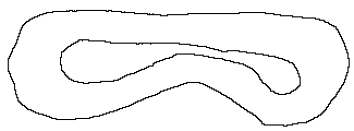
\includegraphics[interpolate=true,width=3.540000in,height=1.310000in]{contents/chapt5/figs/agent/path_end_to_end_agent-img0.png}}%
\end{pgfscope}%
\begin{pgfscope}%
\pgfpathrectangle{\pgfqpoint{1.102617in}{5.442266in}}{\pgfqpoint{3.535955in}{1.305583in}}%
\pgfusepath{clip}%
\pgfsetbuttcap%
\pgfsetroundjoin%
\pgfsetlinewidth{1.505625pt}%
\definecolor{currentstroke}{rgb}{0.501961,0.501961,0.501961}%
\pgfsetstrokecolor{currentstroke}%
\pgfsetdash{{5.550000pt}{2.400000pt}}{0.000000pt}%
\pgfpathmoveto{\pgfqpoint{3.060041in}{6.065888in}}%
\pgfpathlineto{\pgfqpoint{3.144309in}{6.044160in}}%
\pgfpathlineto{\pgfqpoint{3.271407in}{6.014219in}}%
\pgfpathlineto{\pgfqpoint{3.312633in}{6.000745in}}%
\pgfpathlineto{\pgfqpoint{3.373713in}{5.977195in}}%
\pgfpathlineto{\pgfqpoint{3.414267in}{5.960320in}}%
\pgfpathlineto{\pgfqpoint{3.434000in}{5.950943in}}%
\pgfpathlineto{\pgfqpoint{3.453018in}{5.940486in}}%
\pgfpathlineto{\pgfqpoint{3.471058in}{5.928605in}}%
\pgfpathlineto{\pgfqpoint{3.487985in}{5.915134in}}%
\pgfpathlineto{\pgfqpoint{3.553497in}{5.857605in}}%
\pgfpathlineto{\pgfqpoint{3.571697in}{5.845568in}}%
\pgfpathlineto{\pgfqpoint{3.628138in}{5.812289in}}%
\pgfpathlineto{\pgfqpoint{3.645551in}{5.799611in}}%
\pgfpathlineto{\pgfqpoint{3.661460in}{5.785123in}}%
\pgfpathlineto{\pgfqpoint{3.690661in}{5.752815in}}%
\pgfpathlineto{\pgfqpoint{3.705206in}{5.736414in}}%
\pgfpathlineto{\pgfqpoint{3.720551in}{5.720795in}}%
\pgfpathlineto{\pgfqpoint{3.737189in}{5.706559in}}%
\pgfpathlineto{\pgfqpoint{3.755076in}{5.693881in}}%
\pgfpathlineto{\pgfqpoint{3.774037in}{5.682830in}}%
\pgfpathlineto{\pgfqpoint{3.793895in}{5.673472in}}%
\pgfpathlineto{\pgfqpoint{3.814472in}{5.665877in}}%
\pgfpathlineto{\pgfqpoint{3.835598in}{5.660085in}}%
\pgfpathlineto{\pgfqpoint{3.857118in}{5.656027in}}%
\pgfpathlineto{\pgfqpoint{3.878882in}{5.653609in}}%
\pgfpathlineto{\pgfqpoint{3.900740in}{5.652736in}}%
\pgfpathlineto{\pgfqpoint{3.922543in}{5.653313in}}%
\pgfpathlineto{\pgfqpoint{3.965664in}{5.658218in}}%
\pgfpathlineto{\pgfqpoint{4.008445in}{5.666478in}}%
\pgfpathlineto{\pgfqpoint{4.072630in}{5.681543in}}%
\pgfpathlineto{\pgfqpoint{4.093563in}{5.687849in}}%
\pgfpathlineto{\pgfqpoint{4.113876in}{5.695475in}}%
\pgfpathlineto{\pgfqpoint{4.133331in}{5.704841in}}%
\pgfpathlineto{\pgfqpoint{4.151732in}{5.716243in}}%
\pgfpathlineto{\pgfqpoint{4.169047in}{5.729492in}}%
\pgfpathlineto{\pgfqpoint{4.185287in}{5.744275in}}%
\pgfpathlineto{\pgfqpoint{4.200463in}{5.760280in}}%
\pgfpathlineto{\pgfqpoint{4.214585in}{5.777195in}}%
\pgfpathlineto{\pgfqpoint{4.239890in}{5.812809in}}%
\pgfpathlineto{\pgfqpoint{4.262190in}{5.850144in}}%
\pgfpathlineto{\pgfqpoint{4.282600in}{5.888558in}}%
\pgfpathlineto{\pgfqpoint{4.301049in}{5.927973in}}%
\pgfpathlineto{\pgfqpoint{4.316282in}{5.968883in}}%
\pgfpathlineto{\pgfqpoint{4.322275in}{5.990026in}}%
\pgfpathlineto{\pgfqpoint{4.326921in}{6.011526in}}%
\pgfpathlineto{\pgfqpoint{4.330006in}{6.033241in}}%
\pgfpathlineto{\pgfqpoint{4.331315in}{6.055024in}}%
\pgfpathlineto{\pgfqpoint{4.330631in}{6.076732in}}%
\pgfpathlineto{\pgfqpoint{4.327825in}{6.098237in}}%
\pgfpathlineto{\pgfqpoint{4.323108in}{6.119482in}}%
\pgfpathlineto{\pgfqpoint{4.316776in}{6.140428in}}%
\pgfpathlineto{\pgfqpoint{4.300450in}{6.181260in}}%
\pgfpathlineto{\pgfqpoint{4.280599in}{6.220289in}}%
\pgfpathlineto{\pgfqpoint{4.269167in}{6.238835in}}%
\pgfpathlineto{\pgfqpoint{4.256509in}{6.256556in}}%
\pgfpathlineto{\pgfqpoint{4.242457in}{6.273314in}}%
\pgfpathlineto{\pgfqpoint{4.226901in}{6.288947in}}%
\pgfpathlineto{\pgfqpoint{4.209951in}{6.303173in}}%
\pgfpathlineto{\pgfqpoint{4.191769in}{6.315683in}}%
\pgfpathlineto{\pgfqpoint{4.172521in}{6.326168in}}%
\pgfpathlineto{\pgfqpoint{4.152371in}{6.334319in}}%
\pgfpathlineto{\pgfqpoint{4.131495in}{6.340025in}}%
\pgfpathlineto{\pgfqpoint{4.088481in}{6.347023in}}%
\pgfpathlineto{\pgfqpoint{4.045367in}{6.353999in}}%
\pgfpathlineto{\pgfqpoint{4.024301in}{6.359424in}}%
\pgfpathlineto{\pgfqpoint{3.941352in}{6.385904in}}%
\pgfpathlineto{\pgfqpoint{3.920187in}{6.390691in}}%
\pgfpathlineto{\pgfqpoint{3.877156in}{6.397268in}}%
\pgfpathlineto{\pgfqpoint{3.768973in}{6.410045in}}%
\pgfpathlineto{\pgfqpoint{3.639523in}{6.427984in}}%
\pgfpathlineto{\pgfqpoint{3.617837in}{6.428949in}}%
\pgfpathlineto{\pgfqpoint{3.574353in}{6.427530in}}%
\pgfpathlineto{\pgfqpoint{3.530829in}{6.425276in}}%
\pgfpathlineto{\pgfqpoint{3.509097in}{6.425352in}}%
\pgfpathlineto{\pgfqpoint{3.465733in}{6.429170in}}%
\pgfpathlineto{\pgfqpoint{3.422386in}{6.433652in}}%
\pgfpathlineto{\pgfqpoint{3.400670in}{6.434336in}}%
\pgfpathlineto{\pgfqpoint{3.357133in}{6.431145in}}%
\pgfpathlineto{\pgfqpoint{3.313694in}{6.427170in}}%
\pgfpathlineto{\pgfqpoint{3.292110in}{6.427146in}}%
\pgfpathlineto{\pgfqpoint{3.270652in}{6.429346in}}%
\pgfpathlineto{\pgfqpoint{3.227937in}{6.437994in}}%
\pgfpathlineto{\pgfqpoint{3.185106in}{6.446825in}}%
\pgfpathlineto{\pgfqpoint{3.163518in}{6.449445in}}%
\pgfpathlineto{\pgfqpoint{3.120039in}{6.451186in}}%
\pgfpathlineto{\pgfqpoint{2.989241in}{6.450550in}}%
\pgfpathlineto{\pgfqpoint{2.945990in}{6.454856in}}%
\pgfpathlineto{\pgfqpoint{2.881343in}{6.464426in}}%
\pgfpathlineto{\pgfqpoint{2.859735in}{6.466571in}}%
\pgfpathlineto{\pgfqpoint{2.816316in}{6.467498in}}%
\pgfpathlineto{\pgfqpoint{2.642212in}{6.461175in}}%
\pgfpathlineto{\pgfqpoint{2.555263in}{6.455977in}}%
\pgfpathlineto{\pgfqpoint{2.511846in}{6.456514in}}%
\pgfpathlineto{\pgfqpoint{2.381414in}{6.464492in}}%
\pgfpathlineto{\pgfqpoint{2.337939in}{6.466356in}}%
\pgfpathlineto{\pgfqpoint{2.294813in}{6.471454in}}%
\pgfpathlineto{\pgfqpoint{2.209007in}{6.486273in}}%
\pgfpathlineto{\pgfqpoint{2.165645in}{6.489240in}}%
\pgfpathlineto{\pgfqpoint{2.122036in}{6.488941in}}%
\pgfpathlineto{\pgfqpoint{2.034939in}{6.485758in}}%
\pgfpathlineto{\pgfqpoint{2.013190in}{6.486284in}}%
\pgfpathlineto{\pgfqpoint{1.991424in}{6.488072in}}%
\pgfpathlineto{\pgfqpoint{1.904680in}{6.500776in}}%
\pgfpathlineto{\pgfqpoint{1.883354in}{6.500637in}}%
\pgfpathlineto{\pgfqpoint{1.862269in}{6.497504in}}%
\pgfpathlineto{\pgfqpoint{1.841385in}{6.491910in}}%
\pgfpathlineto{\pgfqpoint{1.799979in}{6.476687in}}%
\pgfpathlineto{\pgfqpoint{1.758671in}{6.461472in}}%
\pgfpathlineto{\pgfqpoint{1.655237in}{6.427657in}}%
\pgfpathlineto{\pgfqpoint{1.634911in}{6.419307in}}%
\pgfpathlineto{\pgfqpoint{1.615164in}{6.409825in}}%
\pgfpathlineto{\pgfqpoint{1.596275in}{6.398975in}}%
\pgfpathlineto{\pgfqpoint{1.578519in}{6.386521in}}%
\pgfpathlineto{\pgfqpoint{1.562115in}{6.372314in}}%
\pgfpathlineto{\pgfqpoint{1.547037in}{6.356558in}}%
\pgfpathlineto{\pgfqpoint{1.533197in}{6.339546in}}%
\pgfpathlineto{\pgfqpoint{1.520511in}{6.321569in}}%
\pgfpathlineto{\pgfqpoint{1.498264in}{6.283837in}}%
\pgfpathlineto{\pgfqpoint{1.479876in}{6.244447in}}%
\pgfpathlineto{\pgfqpoint{1.465188in}{6.203285in}}%
\pgfpathlineto{\pgfqpoint{1.459242in}{6.182018in}}%
\pgfpathlineto{\pgfqpoint{1.454510in}{6.160434in}}%
\pgfpathlineto{\pgfqpoint{1.451315in}{6.138698in}}%
\pgfpathlineto{\pgfqpoint{1.449983in}{6.116977in}}%
\pgfpathlineto{\pgfqpoint{1.450838in}{6.095437in}}%
\pgfpathlineto{\pgfqpoint{1.454060in}{6.074201in}}%
\pgfpathlineto{\pgfqpoint{1.459241in}{6.053222in}}%
\pgfpathlineto{\pgfqpoint{1.473273in}{6.011667in}}%
\pgfpathlineto{\pgfqpoint{1.496579in}{5.949506in}}%
\pgfpathlineto{\pgfqpoint{1.505173in}{5.929416in}}%
\pgfpathlineto{\pgfqpoint{1.514943in}{5.910147in}}%
\pgfpathlineto{\pgfqpoint{1.526364in}{5.892009in}}%
\pgfpathlineto{\pgfqpoint{1.539775in}{5.875237in}}%
\pgfpathlineto{\pgfqpoint{1.554960in}{5.859761in}}%
\pgfpathlineto{\pgfqpoint{1.571564in}{5.845436in}}%
\pgfpathlineto{\pgfqpoint{1.589235in}{5.832116in}}%
\pgfpathlineto{\pgfqpoint{1.626423in}{5.807969in}}%
\pgfpathlineto{\pgfqpoint{1.645613in}{5.797213in}}%
\pgfpathlineto{\pgfqpoint{1.665214in}{5.787603in}}%
\pgfpathlineto{\pgfqpoint{1.685252in}{5.779353in}}%
\pgfpathlineto{\pgfqpoint{1.705753in}{5.772681in}}%
\pgfpathlineto{\pgfqpoint{1.726719in}{5.767676in}}%
\pgfpathlineto{\pgfqpoint{1.769637in}{5.760881in}}%
\pgfpathlineto{\pgfqpoint{1.813068in}{5.754774in}}%
\pgfpathlineto{\pgfqpoint{1.899202in}{5.739872in}}%
\pgfpathlineto{\pgfqpoint{1.920664in}{5.738643in}}%
\pgfpathlineto{\pgfqpoint{1.942150in}{5.739473in}}%
\pgfpathlineto{\pgfqpoint{1.985233in}{5.745444in}}%
\pgfpathlineto{\pgfqpoint{2.028512in}{5.752992in}}%
\pgfpathlineto{\pgfqpoint{2.114947in}{5.764683in}}%
\pgfpathlineto{\pgfqpoint{2.136108in}{5.769123in}}%
\pgfpathlineto{\pgfqpoint{2.177644in}{5.781715in}}%
\pgfpathlineto{\pgfqpoint{2.219065in}{5.795406in}}%
\pgfpathlineto{\pgfqpoint{2.240124in}{5.801028in}}%
\pgfpathlineto{\pgfqpoint{2.283203in}{5.808476in}}%
\pgfpathlineto{\pgfqpoint{2.326216in}{5.815445in}}%
\pgfpathlineto{\pgfqpoint{2.347128in}{5.820708in}}%
\pgfpathlineto{\pgfqpoint{2.367401in}{5.827987in}}%
\pgfpathlineto{\pgfqpoint{2.387123in}{5.836991in}}%
\pgfpathlineto{\pgfqpoint{2.425509in}{5.858152in}}%
\pgfpathlineto{\pgfqpoint{2.482561in}{5.890772in}}%
\pgfpathlineto{\pgfqpoint{2.521273in}{5.910480in}}%
\pgfpathlineto{\pgfqpoint{2.561028in}{5.927885in}}%
\pgfpathlineto{\pgfqpoint{2.622202in}{5.950778in}}%
\pgfpathlineto{\pgfqpoint{2.683381in}{5.973566in}}%
\pgfpathlineto{\pgfqpoint{2.743706in}{5.998587in}}%
\pgfpathlineto{\pgfqpoint{2.823670in}{6.033421in}}%
\pgfpathlineto{\pgfqpoint{2.844050in}{6.040638in}}%
\pgfpathlineto{\pgfqpoint{2.864736in}{6.046691in}}%
\pgfpathlineto{\pgfqpoint{2.906954in}{6.055578in}}%
\pgfpathlineto{\pgfqpoint{2.950083in}{6.060999in}}%
\pgfpathlineto{\pgfqpoint{2.993861in}{6.063945in}}%
\pgfpathlineto{\pgfqpoint{3.038030in}{6.065407in}}%
\pgfpathlineto{\pgfqpoint{3.038030in}{6.065407in}}%
\pgfusepath{stroke}%
\end{pgfscope}%
\begin{pgfscope}%
\pgfpathrectangle{\pgfqpoint{1.102617in}{5.442266in}}{\pgfqpoint{3.535955in}{1.305583in}}%
\pgfusepath{clip}%
\pgfsetrectcap%
\pgfsetroundjoin%
\pgfsetlinewidth{1.505625pt}%
\definecolor{currentstroke}{rgb}{0.121569,0.466667,0.705882}%
\pgfsetstrokecolor{currentstroke}%
\pgfsetdash{}{0pt}%
\pgfpathmoveto{\pgfqpoint{3.278589in}{6.421454in}}%
\pgfpathlineto{\pgfqpoint{3.202283in}{6.422374in}}%
\pgfpathlineto{\pgfqpoint{3.132535in}{6.425360in}}%
\pgfpathlineto{\pgfqpoint{3.046730in}{6.431405in}}%
\pgfpathlineto{\pgfqpoint{2.920866in}{6.442596in}}%
\pgfpathlineto{\pgfqpoint{2.812740in}{6.451738in}}%
\pgfpathlineto{\pgfqpoint{2.736033in}{6.456137in}}%
\pgfpathlineto{\pgfqpoint{2.659228in}{6.458252in}}%
\pgfpathlineto{\pgfqpoint{2.494588in}{6.459828in}}%
\pgfpathlineto{\pgfqpoint{2.275062in}{6.460857in}}%
\pgfpathlineto{\pgfqpoint{2.187270in}{6.459083in}}%
\pgfpathlineto{\pgfqpoint{2.110535in}{6.455207in}}%
\pgfpathlineto{\pgfqpoint{2.044910in}{6.449696in}}%
\pgfpathlineto{\pgfqpoint{1.979510in}{6.441959in}}%
\pgfpathlineto{\pgfqpoint{1.914424in}{6.431915in}}%
\pgfpathlineto{\pgfqpoint{1.849741in}{6.419542in}}%
\pgfpathlineto{\pgfqpoint{1.796311in}{6.407026in}}%
\pgfpathlineto{\pgfqpoint{1.764704in}{6.397799in}}%
\pgfpathlineto{\pgfqpoint{1.733715in}{6.386678in}}%
\pgfpathlineto{\pgfqpoint{1.703623in}{6.373322in}}%
\pgfpathlineto{\pgfqpoint{1.674778in}{6.357460in}}%
\pgfpathlineto{\pgfqpoint{1.647612in}{6.338871in}}%
\pgfpathlineto{\pgfqpoint{1.630656in}{6.324934in}}%
\pgfpathlineto{\pgfqpoint{1.614852in}{6.309704in}}%
\pgfpathlineto{\pgfqpoint{1.600359in}{6.293221in}}%
\pgfpathlineto{\pgfqpoint{1.587322in}{6.275565in}}%
\pgfpathlineto{\pgfqpoint{1.575886in}{6.256832in}}%
\pgfpathlineto{\pgfqpoint{1.566191in}{6.237143in}}%
\pgfpathlineto{\pgfqpoint{1.558359in}{6.216641in}}%
\pgfpathlineto{\pgfqpoint{1.552497in}{6.195491in}}%
\pgfpathlineto{\pgfqpoint{1.548689in}{6.173878in}}%
\pgfpathlineto{\pgfqpoint{1.546995in}{6.151997in}}%
\pgfpathlineto{\pgfqpoint{1.547416in}{6.130054in}}%
\pgfpathlineto{\pgfqpoint{1.549833in}{6.108240in}}%
\pgfpathlineto{\pgfqpoint{1.554109in}{6.086712in}}%
\pgfpathlineto{\pgfqpoint{1.560072in}{6.065588in}}%
\pgfpathlineto{\pgfqpoint{1.567615in}{6.044976in}}%
\pgfpathlineto{\pgfqpoint{1.576622in}{6.024958in}}%
\pgfpathlineto{\pgfqpoint{1.592589in}{5.996172in}}%
\pgfpathlineto{\pgfqpoint{1.611121in}{5.968963in}}%
\pgfpathlineto{\pgfqpoint{1.631875in}{5.943407in}}%
\pgfpathlineto{\pgfqpoint{1.654505in}{5.919494in}}%
\pgfpathlineto{\pgfqpoint{1.678734in}{5.897202in}}%
\pgfpathlineto{\pgfqpoint{1.704381in}{5.876555in}}%
\pgfpathlineto{\pgfqpoint{1.731259in}{5.857538in}}%
\pgfpathlineto{\pgfqpoint{1.759229in}{5.840167in}}%
\pgfpathlineto{\pgfqpoint{1.788152in}{5.824434in}}%
\pgfpathlineto{\pgfqpoint{1.817924in}{5.810371in}}%
\pgfpathlineto{\pgfqpoint{1.848479in}{5.798104in}}%
\pgfpathlineto{\pgfqpoint{1.879710in}{5.787678in}}%
\pgfpathlineto{\pgfqpoint{1.911519in}{5.779180in}}%
\pgfpathlineto{\pgfqpoint{1.943793in}{5.772666in}}%
\pgfpathlineto{\pgfqpoint{1.976416in}{5.768218in}}%
\pgfpathlineto{\pgfqpoint{2.009256in}{5.765869in}}%
\pgfpathlineto{\pgfqpoint{2.042181in}{5.765634in}}%
\pgfpathlineto{\pgfqpoint{2.075065in}{5.767285in}}%
\pgfpathlineto{\pgfqpoint{2.107804in}{5.770788in}}%
\pgfpathlineto{\pgfqpoint{2.140311in}{5.776030in}}%
\pgfpathlineto{\pgfqpoint{2.183163in}{5.785557in}}%
\pgfpathlineto{\pgfqpoint{2.225329in}{5.797774in}}%
\pgfpathlineto{\pgfqpoint{2.266717in}{5.812417in}}%
\pgfpathlineto{\pgfqpoint{2.317605in}{5.832962in}}%
\pgfpathlineto{\pgfqpoint{2.377776in}{5.859732in}}%
\pgfpathlineto{\pgfqpoint{2.557648in}{5.941456in}}%
\pgfpathlineto{\pgfqpoint{2.618653in}{5.966266in}}%
\pgfpathlineto{\pgfqpoint{2.680423in}{5.989102in}}%
\pgfpathlineto{\pgfqpoint{2.742946in}{6.009787in}}%
\pgfpathlineto{\pgfqpoint{2.806166in}{6.028232in}}%
\pgfpathlineto{\pgfqpoint{2.859336in}{6.041826in}}%
\pgfpathlineto{\pgfqpoint{2.902273in}{6.050986in}}%
\pgfpathlineto{\pgfqpoint{2.945575in}{6.058221in}}%
\pgfpathlineto{\pgfqpoint{2.989194in}{6.063185in}}%
\pgfpathlineto{\pgfqpoint{3.033029in}{6.065545in}}%
\pgfpathlineto{\pgfqpoint{3.076892in}{6.065095in}}%
\pgfpathlineto{\pgfqpoint{3.120485in}{6.062089in}}%
\pgfpathlineto{\pgfqpoint{3.163654in}{6.056620in}}%
\pgfpathlineto{\pgfqpoint{3.206289in}{6.048863in}}%
\pgfpathlineto{\pgfqpoint{3.248303in}{6.039016in}}%
\pgfpathlineto{\pgfqpoint{3.289528in}{6.027268in}}%
\pgfpathlineto{\pgfqpoint{3.329429in}{6.013663in}}%
\pgfpathlineto{\pgfqpoint{3.367844in}{5.998192in}}%
\pgfpathlineto{\pgfqpoint{3.404615in}{5.980818in}}%
\pgfpathlineto{\pgfqpoint{3.439577in}{5.961541in}}%
\pgfpathlineto{\pgfqpoint{3.472549in}{5.940452in}}%
\pgfpathlineto{\pgfqpoint{3.503398in}{5.917939in}}%
\pgfpathlineto{\pgfqpoint{3.532078in}{5.894204in}}%
\pgfpathlineto{\pgfqpoint{3.558599in}{5.869470in}}%
\pgfpathlineto{\pgfqpoint{3.583013in}{5.843971in}}%
\pgfpathlineto{\pgfqpoint{3.611156in}{5.810892in}}%
\pgfpathlineto{\pgfqpoint{3.662559in}{5.748164in}}%
\pgfpathlineto{\pgfqpoint{3.687978in}{5.720826in}}%
\pgfpathlineto{\pgfqpoint{3.715720in}{5.694685in}}%
\pgfpathlineto{\pgfqpoint{3.738379in}{5.676142in}}%
\pgfpathlineto{\pgfqpoint{3.762928in}{5.658936in}}%
\pgfpathlineto{\pgfqpoint{3.789375in}{5.643388in}}%
\pgfpathlineto{\pgfqpoint{3.817654in}{5.629790in}}%
\pgfpathlineto{\pgfqpoint{3.847668in}{5.618469in}}%
\pgfpathlineto{\pgfqpoint{3.879178in}{5.609726in}}%
\pgfpathlineto{\pgfqpoint{3.911454in}{5.604021in}}%
\pgfpathlineto{\pgfqpoint{3.933219in}{5.602021in}}%
\pgfpathlineto{\pgfqpoint{3.955069in}{5.601543in}}%
\pgfpathlineto{\pgfqpoint{3.976896in}{5.602669in}}%
\pgfpathlineto{\pgfqpoint{3.998573in}{5.605454in}}%
\pgfpathlineto{\pgfqpoint{4.019965in}{5.609928in}}%
\pgfpathlineto{\pgfqpoint{4.040931in}{5.616097in}}%
\pgfpathlineto{\pgfqpoint{4.061327in}{5.623946in}}%
\pgfpathlineto{\pgfqpoint{4.081012in}{5.633440in}}%
\pgfpathlineto{\pgfqpoint{4.099845in}{5.644528in}}%
\pgfpathlineto{\pgfqpoint{4.117684in}{5.657135in}}%
\pgfpathlineto{\pgfqpoint{4.134442in}{5.671081in}}%
\pgfpathlineto{\pgfqpoint{4.150098in}{5.686193in}}%
\pgfpathlineto{\pgfqpoint{4.171527in}{5.710699in}}%
\pgfpathlineto{\pgfqpoint{4.190442in}{5.737078in}}%
\pgfpathlineto{\pgfqpoint{4.206871in}{5.764964in}}%
\pgfpathlineto{\pgfqpoint{4.220944in}{5.794005in}}%
\pgfpathlineto{\pgfqpoint{4.232774in}{5.823928in}}%
\pgfpathlineto{\pgfqpoint{4.242473in}{5.854570in}}%
\pgfpathlineto{\pgfqpoint{4.249904in}{5.885832in}}%
\pgfpathlineto{\pgfqpoint{4.255102in}{5.917533in}}%
\pgfpathlineto{\pgfqpoint{4.258017in}{5.949518in}}%
\pgfpathlineto{\pgfqpoint{4.258615in}{5.981622in}}%
\pgfpathlineto{\pgfqpoint{4.256833in}{6.013674in}}%
\pgfpathlineto{\pgfqpoint{4.252653in}{6.045551in}}%
\pgfpathlineto{\pgfqpoint{4.245913in}{6.077444in}}%
\pgfpathlineto{\pgfqpoint{4.236459in}{6.108815in}}%
\pgfpathlineto{\pgfqpoint{4.224360in}{6.139262in}}%
\pgfpathlineto{\pgfqpoint{4.209542in}{6.168482in}}%
\pgfpathlineto{\pgfqpoint{4.191978in}{6.196137in}}%
\pgfpathlineto{\pgfqpoint{4.178747in}{6.213520in}}%
\pgfpathlineto{\pgfqpoint{4.164335in}{6.229936in}}%
\pgfpathlineto{\pgfqpoint{4.148787in}{6.245281in}}%
\pgfpathlineto{\pgfqpoint{4.123622in}{6.266259in}}%
\pgfpathlineto{\pgfqpoint{4.096646in}{6.284853in}}%
\pgfpathlineto{\pgfqpoint{4.068169in}{6.301058in}}%
\pgfpathlineto{\pgfqpoint{4.038478in}{6.314915in}}%
\pgfpathlineto{\pgfqpoint{4.007851in}{6.326561in}}%
\pgfpathlineto{\pgfqpoint{3.976502in}{6.336100in}}%
\pgfpathlineto{\pgfqpoint{3.944637in}{6.343747in}}%
\pgfpathlineto{\pgfqpoint{3.901692in}{6.351797in}}%
\pgfpathlineto{\pgfqpoint{3.847605in}{6.359399in}}%
\pgfpathlineto{\pgfqpoint{3.760695in}{6.368570in}}%
\pgfpathlineto{\pgfqpoint{3.586799in}{6.386193in}}%
\pgfpathlineto{\pgfqpoint{3.434950in}{6.404422in}}%
\pgfpathlineto{\pgfqpoint{3.337301in}{6.415876in}}%
\pgfpathlineto{\pgfqpoint{3.337301in}{6.415876in}}%
\pgfusepath{stroke}%
\end{pgfscope}%
\begin{pgfscope}%
\pgfpathrectangle{\pgfqpoint{1.102617in}{5.442266in}}{\pgfqpoint{3.535955in}{1.305583in}}%
\pgfusepath{clip}%
\pgfsetbuttcap%
\pgfsetroundjoin%
\pgfsetlinewidth{1.505625pt}%
\definecolor{currentstroke}{rgb}{1.000000,0.000000,0.000000}%
\pgfsetstrokecolor{currentstroke}%
\pgfsetdash{{1.500000pt}{2.475000pt}}{0.000000pt}%
\pgfpathmoveto{\pgfqpoint{3.270652in}{6.211749in}}%
\pgfpathlineto{\pgfqpoint{3.270652in}{6.646943in}}%
\pgfusepath{stroke}%
\end{pgfscope}%
\begin{pgfscope}%
\pgfsetbuttcap%
\pgfsetmiterjoin%
\definecolor{currentfill}{rgb}{1.000000,1.000000,1.000000}%
\pgfsetfillcolor{currentfill}%
\pgfsetlinewidth{1.003750pt}%
\definecolor{currentstroke}{rgb}{0.000000,0.000000,0.000000}%
\pgfsetstrokecolor{currentstroke}%
\pgfsetdash{}{0pt}%
\pgfpathmoveto{\pgfqpoint{1.926208in}{6.457787in}}%
\pgfpathlineto{\pgfqpoint{2.180690in}{6.457787in}}%
\pgfpathquadraticcurveto{\pgfqpoint{2.194573in}{6.457787in}}{\pgfqpoint{2.194573in}{6.471670in}}%
\pgfpathlineto{\pgfqpoint{2.194573in}{6.594954in}}%
\pgfpathquadraticcurveto{\pgfqpoint{2.194573in}{6.608837in}}{\pgfqpoint{2.180690in}{6.608837in}}%
\pgfpathlineto{\pgfqpoint{1.926208in}{6.608837in}}%
\pgfpathquadraticcurveto{\pgfqpoint{1.912325in}{6.608837in}}{\pgfqpoint{1.912325in}{6.594954in}}%
\pgfpathlineto{\pgfqpoint{1.912325in}{6.471670in}}%
\pgfpathquadraticcurveto{\pgfqpoint{1.912325in}{6.457787in}}{\pgfqpoint{1.926208in}{6.457787in}}%
\pgfpathlineto{\pgfqpoint{1.926208in}{6.457787in}}%
\pgfpathclose%
\pgfusepath{stroke,fill}%
\end{pgfscope}%
\begin{pgfscope}%
\definecolor{textcolor}{rgb}{0.000000,0.000000,0.000000}%
\pgfsetstrokecolor{textcolor}%
\pgfsetfillcolor{textcolor}%
\pgftext[x=1.926208in,y=6.498604in,left,base]{\color{textcolor}\rmfamily\fontsize{9.996000}{11.995200}\selectfont 20\%}%
\end{pgfscope}%
\begin{pgfscope}%
\pgfsetbuttcap%
\pgfsetmiterjoin%
\definecolor{currentfill}{rgb}{1.000000,1.000000,1.000000}%
\pgfsetfillcolor{currentfill}%
\pgfsetlinewidth{1.003750pt}%
\definecolor{currentstroke}{rgb}{0.000000,0.000000,0.000000}%
\pgfsetstrokecolor{currentstroke}%
\pgfsetdash{}{0pt}%
\pgfpathmoveto{\pgfqpoint{1.920664in}{5.697826in}}%
\pgfpathlineto{\pgfqpoint{2.175146in}{5.697826in}}%
\pgfpathquadraticcurveto{\pgfqpoint{2.189029in}{5.697826in}}{\pgfqpoint{2.189029in}{5.711709in}}%
\pgfpathlineto{\pgfqpoint{2.189029in}{5.834993in}}%
\pgfpathquadraticcurveto{\pgfqpoint{2.189029in}{5.848876in}}{\pgfqpoint{2.175146in}{5.848876in}}%
\pgfpathlineto{\pgfqpoint{1.920664in}{5.848876in}}%
\pgfpathquadraticcurveto{\pgfqpoint{1.906781in}{5.848876in}}{\pgfqpoint{1.906781in}{5.834993in}}%
\pgfpathlineto{\pgfqpoint{1.906781in}{5.711709in}}%
\pgfpathquadraticcurveto{\pgfqpoint{1.906781in}{5.697826in}}{\pgfqpoint{1.920664in}{5.697826in}}%
\pgfpathlineto{\pgfqpoint{1.920664in}{5.697826in}}%
\pgfpathclose%
\pgfusepath{stroke,fill}%
\end{pgfscope}%
\begin{pgfscope}%
\definecolor{textcolor}{rgb}{0.000000,0.000000,0.000000}%
\pgfsetstrokecolor{textcolor}%
\pgfsetfillcolor{textcolor}%
\pgftext[x=1.920664in,y=5.738643in,left,base]{\color{textcolor}\rmfamily\fontsize{9.996000}{11.995200}\selectfont 40\%}%
\end{pgfscope}%
\begin{pgfscope}%
\pgfsetbuttcap%
\pgfsetmiterjoin%
\definecolor{currentfill}{rgb}{1.000000,1.000000,1.000000}%
\pgfsetfillcolor{currentfill}%
\pgfsetlinewidth{1.003750pt}%
\definecolor{currentstroke}{rgb}{0.000000,0.000000,0.000000}%
\pgfsetstrokecolor{currentstroke}%
\pgfsetdash{}{0pt}%
\pgfpathmoveto{\pgfqpoint{3.208086in}{5.988996in}}%
\pgfpathlineto{\pgfqpoint{3.462567in}{5.988996in}}%
\pgfpathquadraticcurveto{\pgfqpoint{3.476451in}{5.988996in}}{\pgfqpoint{3.476451in}{6.002879in}}%
\pgfpathlineto{\pgfqpoint{3.476451in}{6.126163in}}%
\pgfpathquadraticcurveto{\pgfqpoint{3.476451in}{6.140046in}}{\pgfqpoint{3.462567in}{6.140046in}}%
\pgfpathlineto{\pgfqpoint{3.208086in}{6.140046in}}%
\pgfpathquadraticcurveto{\pgfqpoint{3.194202in}{6.140046in}}{\pgfqpoint{3.194202in}{6.126163in}}%
\pgfpathlineto{\pgfqpoint{3.194202in}{6.002879in}}%
\pgfpathquadraticcurveto{\pgfqpoint{3.194202in}{5.988996in}}{\pgfqpoint{3.208086in}{5.988996in}}%
\pgfpathlineto{\pgfqpoint{3.208086in}{5.988996in}}%
\pgfpathclose%
\pgfusepath{stroke,fill}%
\end{pgfscope}%
\begin{pgfscope}%
\definecolor{textcolor}{rgb}{0.000000,0.000000,0.000000}%
\pgfsetstrokecolor{textcolor}%
\pgfsetfillcolor{textcolor}%
\pgftext[x=3.208086in,y=6.029812in,left,base]{\color{textcolor}\rmfamily\fontsize{9.996000}{11.995200}\selectfont 60\%}%
\end{pgfscope}%
\begin{pgfscope}%
\pgfsetbuttcap%
\pgfsetmiterjoin%
\definecolor{currentfill}{rgb}{1.000000,1.000000,1.000000}%
\pgfsetfillcolor{currentfill}%
\pgfsetlinewidth{1.003750pt}%
\definecolor{currentstroke}{rgb}{0.000000,0.000000,0.000000}%
\pgfsetstrokecolor{currentstroke}%
\pgfsetdash{}{0pt}%
\pgfpathmoveto{\pgfqpoint{4.309149in}{5.907392in}}%
\pgfpathlineto{\pgfqpoint{4.563631in}{5.907392in}}%
\pgfpathquadraticcurveto{\pgfqpoint{4.577514in}{5.907392in}}{\pgfqpoint{4.577514in}{5.921276in}}%
\pgfpathlineto{\pgfqpoint{4.577514in}{6.044560in}}%
\pgfpathquadraticcurveto{\pgfqpoint{4.577514in}{6.058443in}}{\pgfqpoint{4.563631in}{6.058443in}}%
\pgfpathlineto{\pgfqpoint{4.309149in}{6.058443in}}%
\pgfpathquadraticcurveto{\pgfqpoint{4.295266in}{6.058443in}}{\pgfqpoint{4.295266in}{6.044560in}}%
\pgfpathlineto{\pgfqpoint{4.295266in}{5.921276in}}%
\pgfpathquadraticcurveto{\pgfqpoint{4.295266in}{5.907392in}}{\pgfqpoint{4.309149in}{5.907392in}}%
\pgfpathlineto{\pgfqpoint{4.309149in}{5.907392in}}%
\pgfpathclose%
\pgfusepath{stroke,fill}%
\end{pgfscope}%
\begin{pgfscope}%
\definecolor{textcolor}{rgb}{0.000000,0.000000,0.000000}%
\pgfsetstrokecolor{textcolor}%
\pgfsetfillcolor{textcolor}%
\pgftext[x=4.309149in,y=5.948209in,left,base]{\color{textcolor}\rmfamily\fontsize{9.996000}{11.995200}\selectfont 80\%}%
\end{pgfscope}%
\begin{pgfscope}%
\pgfsetbuttcap%
\pgfsetmiterjoin%
\definecolor{currentfill}{rgb}{1.000000,1.000000,1.000000}%
\pgfsetfillcolor{currentfill}%
\pgfsetlinewidth{1.003750pt}%
\definecolor{currentstroke}{rgb}{0.000000,0.000000,0.000000}%
\pgfsetstrokecolor{currentstroke}%
\pgfsetdash{}{0pt}%
\pgfpathmoveto{\pgfqpoint{3.009535in}{6.663631in}}%
\pgfpathlineto{\pgfqpoint{3.712865in}{6.663631in}}%
\pgfpathquadraticcurveto{\pgfqpoint{3.726749in}{6.663631in}}{\pgfqpoint{3.726749in}{6.677514in}}%
\pgfpathlineto{\pgfqpoint{3.726749in}{6.816348in}}%
\pgfpathquadraticcurveto{\pgfqpoint{3.726749in}{6.830231in}}{\pgfqpoint{3.712865in}{6.830231in}}%
\pgfpathlineto{\pgfqpoint{3.009535in}{6.830231in}}%
\pgfpathquadraticcurveto{\pgfqpoint{2.995652in}{6.830231in}}{\pgfqpoint{2.995652in}{6.816348in}}%
\pgfpathlineto{\pgfqpoint{2.995652in}{6.677514in}}%
\pgfpathquadraticcurveto{\pgfqpoint{2.995652in}{6.663631in}}{\pgfqpoint{3.009535in}{6.663631in}}%
\pgfpathlineto{\pgfqpoint{3.009535in}{6.663631in}}%
\pgfpathclose%
\pgfusepath{stroke,fill}%
\end{pgfscope}%
\begin{pgfscope}%
\definecolor{textcolor}{rgb}{0.000000,0.000000,0.000000}%
\pgfsetstrokecolor{textcolor}%
\pgfsetfillcolor{textcolor}%
\pgftext[x=3.009535in,y=6.712222in,left,base]{\color{textcolor}\rmfamily\fontsize{9.996000}{11.995200}\selectfont Start/finish}%
\end{pgfscope}%
\begin{pgfscope}%
\pgfsetbuttcap%
\pgfsetmiterjoin%
\definecolor{currentfill}{rgb}{1.000000,1.000000,1.000000}%
\pgfsetfillcolor{currentfill}%
\pgfsetlinewidth{0.000000pt}%
\definecolor{currentstroke}{rgb}{0.000000,0.000000,0.000000}%
\pgfsetstrokecolor{currentstroke}%
\pgfsetstrokeopacity{0.000000}%
\pgfsetdash{}{0pt}%
\pgfpathmoveto{\pgfqpoint{1.043583in}{3.908178in}}%
\pgfpathlineto{\pgfqpoint{4.697605in}{3.908178in}}%
\pgfpathlineto{\pgfqpoint{4.697605in}{5.213761in}}%
\pgfpathlineto{\pgfqpoint{1.043583in}{5.213761in}}%
\pgfpathlineto{\pgfqpoint{1.043583in}{3.908178in}}%
\pgfpathclose%
\pgfusepath{fill}%
\end{pgfscope}%
\begin{pgfscope}%
\pgfpathrectangle{\pgfqpoint{1.043583in}{3.908178in}}{\pgfqpoint{3.654022in}{1.305583in}}%
\pgfusepath{clip}%
\pgfsetrectcap%
\pgfsetroundjoin%
\pgfsetlinewidth{0.803000pt}%
\definecolor{currentstroke}{rgb}{0.827451,0.827451,0.827451}%
\pgfsetstrokecolor{currentstroke}%
\pgfsetdash{}{0pt}%
\pgfpathmoveto{\pgfqpoint{1.043583in}{3.908178in}}%
\pgfpathlineto{\pgfqpoint{1.043583in}{5.213761in}}%
\pgfusepath{stroke}%
\end{pgfscope}%
\begin{pgfscope}%
\pgfpathrectangle{\pgfqpoint{1.043583in}{3.908178in}}{\pgfqpoint{3.654022in}{1.305583in}}%
\pgfusepath{clip}%
\pgfsetrectcap%
\pgfsetroundjoin%
\pgfsetlinewidth{0.803000pt}%
\definecolor{currentstroke}{rgb}{0.827451,0.827451,0.827451}%
\pgfsetstrokecolor{currentstroke}%
\pgfsetdash{}{0pt}%
\pgfpathmoveto{\pgfqpoint{1.774388in}{3.908178in}}%
\pgfpathlineto{\pgfqpoint{1.774388in}{5.213761in}}%
\pgfusepath{stroke}%
\end{pgfscope}%
\begin{pgfscope}%
\pgfpathrectangle{\pgfqpoint{1.043583in}{3.908178in}}{\pgfqpoint{3.654022in}{1.305583in}}%
\pgfusepath{clip}%
\pgfsetrectcap%
\pgfsetroundjoin%
\pgfsetlinewidth{0.803000pt}%
\definecolor{currentstroke}{rgb}{0.827451,0.827451,0.827451}%
\pgfsetstrokecolor{currentstroke}%
\pgfsetdash{}{0pt}%
\pgfpathmoveto{\pgfqpoint{2.505192in}{3.908178in}}%
\pgfpathlineto{\pgfqpoint{2.505192in}{5.213761in}}%
\pgfusepath{stroke}%
\end{pgfscope}%
\begin{pgfscope}%
\pgfpathrectangle{\pgfqpoint{1.043583in}{3.908178in}}{\pgfqpoint{3.654022in}{1.305583in}}%
\pgfusepath{clip}%
\pgfsetrectcap%
\pgfsetroundjoin%
\pgfsetlinewidth{0.803000pt}%
\definecolor{currentstroke}{rgb}{0.827451,0.827451,0.827451}%
\pgfsetstrokecolor{currentstroke}%
\pgfsetdash{}{0pt}%
\pgfpathmoveto{\pgfqpoint{3.235997in}{3.908178in}}%
\pgfpathlineto{\pgfqpoint{3.235997in}{5.213761in}}%
\pgfusepath{stroke}%
\end{pgfscope}%
\begin{pgfscope}%
\pgfpathrectangle{\pgfqpoint{1.043583in}{3.908178in}}{\pgfqpoint{3.654022in}{1.305583in}}%
\pgfusepath{clip}%
\pgfsetrectcap%
\pgfsetroundjoin%
\pgfsetlinewidth{0.803000pt}%
\definecolor{currentstroke}{rgb}{0.827451,0.827451,0.827451}%
\pgfsetstrokecolor{currentstroke}%
\pgfsetdash{}{0pt}%
\pgfpathmoveto{\pgfqpoint{3.966801in}{3.908178in}}%
\pgfpathlineto{\pgfqpoint{3.966801in}{5.213761in}}%
\pgfusepath{stroke}%
\end{pgfscope}%
\begin{pgfscope}%
\pgfpathrectangle{\pgfqpoint{1.043583in}{3.908178in}}{\pgfqpoint{3.654022in}{1.305583in}}%
\pgfusepath{clip}%
\pgfsetrectcap%
\pgfsetroundjoin%
\pgfsetlinewidth{0.803000pt}%
\definecolor{currentstroke}{rgb}{0.827451,0.827451,0.827451}%
\pgfsetstrokecolor{currentstroke}%
\pgfsetdash{}{0pt}%
\pgfpathmoveto{\pgfqpoint{4.697605in}{3.908178in}}%
\pgfpathlineto{\pgfqpoint{4.697605in}{5.213761in}}%
\pgfusepath{stroke}%
\end{pgfscope}%
\begin{pgfscope}%
\pgfpathrectangle{\pgfqpoint{1.043583in}{3.908178in}}{\pgfqpoint{3.654022in}{1.305583in}}%
\pgfusepath{clip}%
\pgfsetrectcap%
\pgfsetroundjoin%
\pgfsetlinewidth{0.803000pt}%
\definecolor{currentstroke}{rgb}{0.827451,0.827451,0.827451}%
\pgfsetstrokecolor{currentstroke}%
\pgfsetdash{}{0pt}%
\pgfpathmoveto{\pgfqpoint{1.043583in}{4.016976in}}%
\pgfpathlineto{\pgfqpoint{4.697605in}{4.016976in}}%
\pgfusepath{stroke}%
\end{pgfscope}%
\begin{pgfscope}%
\definecolor{textcolor}{rgb}{0.000000,0.000000,0.000000}%
\pgfsetstrokecolor{textcolor}%
\pgfsetfillcolor{textcolor}%
\pgftext[x=0.913376in, y=3.959143in, left, base]{\color{textcolor}\rmfamily\fontsize{12.000000}{14.400000}\selectfont \(\displaystyle {3}\)}%
\end{pgfscope}%
\begin{pgfscope}%
\pgfpathrectangle{\pgfqpoint{1.043583in}{3.908178in}}{\pgfqpoint{3.654022in}{1.305583in}}%
\pgfusepath{clip}%
\pgfsetrectcap%
\pgfsetroundjoin%
\pgfsetlinewidth{0.803000pt}%
\definecolor{currentstroke}{rgb}{0.827451,0.827451,0.827451}%
\pgfsetstrokecolor{currentstroke}%
\pgfsetdash{}{0pt}%
\pgfpathmoveto{\pgfqpoint{1.043583in}{4.560969in}}%
\pgfpathlineto{\pgfqpoint{4.697605in}{4.560969in}}%
\pgfusepath{stroke}%
\end{pgfscope}%
\begin{pgfscope}%
\definecolor{textcolor}{rgb}{0.000000,0.000000,0.000000}%
\pgfsetstrokecolor{textcolor}%
\pgfsetfillcolor{textcolor}%
\pgftext[x=0.913376in, y=4.503136in, left, base]{\color{textcolor}\rmfamily\fontsize{12.000000}{14.400000}\selectfont \(\displaystyle {4}\)}%
\end{pgfscope}%
\begin{pgfscope}%
\pgfpathrectangle{\pgfqpoint{1.043583in}{3.908178in}}{\pgfqpoint{3.654022in}{1.305583in}}%
\pgfusepath{clip}%
\pgfsetrectcap%
\pgfsetroundjoin%
\pgfsetlinewidth{0.803000pt}%
\definecolor{currentstroke}{rgb}{0.827451,0.827451,0.827451}%
\pgfsetstrokecolor{currentstroke}%
\pgfsetdash{}{0pt}%
\pgfpathmoveto{\pgfqpoint{1.043583in}{5.104962in}}%
\pgfpathlineto{\pgfqpoint{4.697605in}{5.104962in}}%
\pgfusepath{stroke}%
\end{pgfscope}%
\begin{pgfscope}%
\definecolor{textcolor}{rgb}{0.000000,0.000000,0.000000}%
\pgfsetstrokecolor{textcolor}%
\pgfsetfillcolor{textcolor}%
\pgftext[x=0.913376in, y=5.047129in, left, base]{\color{textcolor}\rmfamily\fontsize{12.000000}{14.400000}\selectfont \(\displaystyle {5}\)}%
\end{pgfscope}%
\begin{pgfscope}%
\definecolor{textcolor}{rgb}{0.000000,0.000000,0.000000}%
\pgfsetstrokecolor{textcolor}%
\pgfsetfillcolor{textcolor}%
\pgftext[x=0.631987in, y=4.106386in, left, base,rotate=90.000000]{\color{textcolor}\rmfamily\fontsize{12.000000}{14.400000}\selectfont Longitudinal}%
\end{pgfscope}%
\begin{pgfscope}%
\definecolor{textcolor}{rgb}{0.000000,0.000000,0.000000}%
\pgfsetstrokecolor{textcolor}%
\pgfsetfillcolor{textcolor}%
\pgftext[x=0.816154in, y=4.073136in, left, base,rotate=90.000000]{\color{textcolor}\rmfamily\fontsize{12.000000}{14.400000}\selectfont velocity [m/s]}%
\end{pgfscope}%
\begin{pgfscope}%
\pgfpathrectangle{\pgfqpoint{1.043583in}{3.908178in}}{\pgfqpoint{3.654022in}{1.305583in}}%
\pgfusepath{clip}%
\pgfsetbuttcap%
\pgfsetroundjoin%
\pgfsetlinewidth{1.505625pt}%
\definecolor{currentstroke}{rgb}{0.000000,0.000000,0.000000}%
\pgfsetstrokecolor{currentstroke}%
\pgfsetdash{{5.550000pt}{2.400000pt}}{0.000000pt}%
\pgfpathmoveto{\pgfqpoint{1.043583in}{4.016976in}}%
\pgfpathlineto{\pgfqpoint{4.697605in}{4.016976in}}%
\pgfusepath{stroke}%
\end{pgfscope}%
\begin{pgfscope}%
\pgfpathrectangle{\pgfqpoint{1.043583in}{3.908178in}}{\pgfqpoint{3.654022in}{1.305583in}}%
\pgfusepath{clip}%
\pgfsetbuttcap%
\pgfsetroundjoin%
\pgfsetlinewidth{1.505625pt}%
\definecolor{currentstroke}{rgb}{0.000000,0.000000,0.000000}%
\pgfsetstrokecolor{currentstroke}%
\pgfsetdash{{5.550000pt}{2.400000pt}}{0.000000pt}%
\pgfpathmoveto{\pgfqpoint{1.043583in}{5.104962in}}%
\pgfpathlineto{\pgfqpoint{4.697605in}{5.104962in}}%
\pgfusepath{stroke}%
\end{pgfscope}%
\begin{pgfscope}%
\pgfpathrectangle{\pgfqpoint{1.043583in}{3.908178in}}{\pgfqpoint{3.654022in}{1.305583in}}%
\pgfusepath{clip}%
\pgfsetrectcap%
\pgfsetroundjoin%
\pgfsetlinewidth{1.505625pt}%
\definecolor{currentstroke}{rgb}{0.121569,0.466667,0.705882}%
\pgfsetstrokecolor{currentstroke}%
\pgfsetdash{}{0pt}%
\pgfpathmoveto{\pgfqpoint{1.043583in}{4.016976in}}%
\pgfpathlineto{\pgfqpoint{1.043583in}{4.078439in}}%
\pgfpathlineto{\pgfqpoint{1.055371in}{4.098926in}}%
\pgfpathlineto{\pgfqpoint{1.055371in}{4.139901in}}%
\pgfpathlineto{\pgfqpoint{1.067158in}{4.160389in}}%
\pgfpathlineto{\pgfqpoint{1.067158in}{4.201364in}}%
\pgfpathlineto{\pgfqpoint{1.078945in}{4.221851in}}%
\pgfpathlineto{\pgfqpoint{1.078945in}{4.262826in}}%
\pgfpathlineto{\pgfqpoint{1.090732in}{4.283314in}}%
\pgfpathlineto{\pgfqpoint{1.090732in}{4.324289in}}%
\pgfpathlineto{\pgfqpoint{1.102519in}{4.344777in}}%
\pgfpathlineto{\pgfqpoint{1.102519in}{4.365264in}}%
\pgfpathlineto{\pgfqpoint{1.114306in}{4.385752in}}%
\pgfpathlineto{\pgfqpoint{1.114306in}{4.426727in}}%
\pgfpathlineto{\pgfqpoint{1.126094in}{4.450894in}}%
\pgfpathlineto{\pgfqpoint{1.126094in}{4.475061in}}%
\pgfpathlineto{\pgfqpoint{1.137881in}{4.499228in}}%
\pgfpathlineto{\pgfqpoint{1.137881in}{4.547562in}}%
\pgfpathlineto{\pgfqpoint{1.149668in}{4.571729in}}%
\pgfpathlineto{\pgfqpoint{1.149668in}{4.595896in}}%
\pgfpathlineto{\pgfqpoint{1.161455in}{4.620063in}}%
\pgfpathlineto{\pgfqpoint{1.161455in}{4.668398in}}%
\pgfpathlineto{\pgfqpoint{1.173242in}{4.692565in}}%
\pgfpathlineto{\pgfqpoint{1.173242in}{4.716732in}}%
\pgfpathlineto{\pgfqpoint{1.185029in}{4.740899in}}%
\pgfpathlineto{\pgfqpoint{1.185029in}{4.789233in}}%
\pgfpathlineto{\pgfqpoint{1.196817in}{4.813400in}}%
\pgfpathlineto{\pgfqpoint{1.196817in}{4.837567in}}%
\pgfpathlineto{\pgfqpoint{1.208604in}{4.861735in}}%
\pgfpathlineto{\pgfqpoint{1.208604in}{4.885902in}}%
\pgfpathlineto{\pgfqpoint{1.220391in}{4.910069in}}%
\pgfpathlineto{\pgfqpoint{1.220391in}{4.941364in}}%
\pgfpathlineto{\pgfqpoint{1.232178in}{4.972659in}}%
\pgfpathlineto{\pgfqpoint{1.232178in}{5.003954in}}%
\pgfpathlineto{\pgfqpoint{1.243965in}{5.035249in}}%
\pgfpathlineto{\pgfqpoint{1.243965in}{5.066544in}}%
\pgfpathlineto{\pgfqpoint{1.255752in}{5.097839in}}%
\pgfpathlineto{\pgfqpoint{1.255752in}{5.129134in}}%
\pgfpathlineto{\pgfqpoint{3.141699in}{5.129134in}}%
\pgfpathlineto{\pgfqpoint{3.141699in}{5.129134in}}%
\pgfpathlineto{\pgfqpoint{3.153486in}{5.126296in}}%
\pgfpathlineto{\pgfqpoint{3.153486in}{5.123458in}}%
\pgfpathlineto{\pgfqpoint{3.165274in}{5.120620in}}%
\pgfpathlineto{\pgfqpoint{3.165274in}{5.117782in}}%
\pgfpathlineto{\pgfqpoint{3.177061in}{5.114944in}}%
\pgfpathlineto{\pgfqpoint{3.177061in}{5.112107in}}%
\pgfpathlineto{\pgfqpoint{3.188848in}{5.109269in}}%
\pgfpathlineto{\pgfqpoint{3.188848in}{5.106431in}}%
\pgfpathlineto{\pgfqpoint{3.200635in}{5.103593in}}%
\pgfpathlineto{\pgfqpoint{3.200635in}{5.100755in}}%
\pgfpathlineto{\pgfqpoint{3.212422in}{5.097917in}}%
\pgfpathlineto{\pgfqpoint{3.212422in}{5.095079in}}%
\pgfpathlineto{\pgfqpoint{3.224209in}{5.092241in}}%
\pgfpathlineto{\pgfqpoint{3.224209in}{5.089403in}}%
\pgfpathlineto{\pgfqpoint{3.235997in}{5.086565in}}%
\pgfpathlineto{\pgfqpoint{3.235997in}{5.083727in}}%
\pgfpathlineto{\pgfqpoint{3.247784in}{5.080889in}}%
\pgfpathlineto{\pgfqpoint{3.247784in}{5.078051in}}%
\pgfpathlineto{\pgfqpoint{3.259571in}{5.075213in}}%
\pgfpathlineto{\pgfqpoint{3.259571in}{5.072375in}}%
\pgfpathlineto{\pgfqpoint{3.271358in}{5.060756in}}%
\pgfpathlineto{\pgfqpoint{3.271358in}{5.049138in}}%
\pgfpathlineto{\pgfqpoint{3.283145in}{5.037519in}}%
\pgfpathlineto{\pgfqpoint{3.283145in}{5.025900in}}%
\pgfpathlineto{\pgfqpoint{3.294932in}{5.014281in}}%
\pgfpathlineto{\pgfqpoint{3.294932in}{5.002663in}}%
\pgfpathlineto{\pgfqpoint{3.306720in}{4.991044in}}%
\pgfpathlineto{\pgfqpoint{3.306720in}{4.967806in}}%
\pgfpathlineto{\pgfqpoint{3.318507in}{4.956188in}}%
\pgfpathlineto{\pgfqpoint{3.318507in}{4.944569in}}%
\pgfpathlineto{\pgfqpoint{3.330294in}{4.932950in}}%
\pgfpathlineto{\pgfqpoint{3.330294in}{4.921332in}}%
\pgfpathlineto{\pgfqpoint{3.342081in}{4.909713in}}%
\pgfpathlineto{\pgfqpoint{3.342081in}{4.898094in}}%
\pgfpathlineto{\pgfqpoint{3.353868in}{4.886475in}}%
\pgfpathlineto{\pgfqpoint{3.353868in}{4.874857in}}%
\pgfpathlineto{\pgfqpoint{3.365655in}{4.863238in}}%
\pgfpathlineto{\pgfqpoint{3.365655in}{4.840000in}}%
\pgfpathlineto{\pgfqpoint{3.377443in}{4.824950in}}%
\pgfpathlineto{\pgfqpoint{3.377443in}{4.809899in}}%
\pgfpathlineto{\pgfqpoint{3.389230in}{4.794848in}}%
\pgfpathlineto{\pgfqpoint{3.389230in}{4.779797in}}%
\pgfpathlineto{\pgfqpoint{3.401017in}{4.764746in}}%
\pgfpathlineto{\pgfqpoint{3.401017in}{4.734645in}}%
\pgfpathlineto{\pgfqpoint{3.412804in}{4.719594in}}%
\pgfpathlineto{\pgfqpoint{3.412804in}{4.704543in}}%
\pgfpathlineto{\pgfqpoint{3.424591in}{4.689492in}}%
\pgfpathlineto{\pgfqpoint{3.424591in}{4.674441in}}%
\pgfpathlineto{\pgfqpoint{3.436378in}{4.659390in}}%
\pgfpathlineto{\pgfqpoint{3.436378in}{4.629289in}}%
\pgfpathlineto{\pgfqpoint{3.448166in}{4.614238in}}%
\pgfpathlineto{\pgfqpoint{3.448166in}{4.599187in}}%
\pgfpathlineto{\pgfqpoint{3.459953in}{4.584136in}}%
\pgfpathlineto{\pgfqpoint{3.459953in}{4.554035in}}%
\pgfpathlineto{\pgfqpoint{3.471740in}{4.538984in}}%
\pgfpathlineto{\pgfqpoint{3.471740in}{4.551356in}}%
\pgfpathlineto{\pgfqpoint{3.483527in}{4.563727in}}%
\pgfpathlineto{\pgfqpoint{3.483527in}{4.588471in}}%
\pgfpathlineto{\pgfqpoint{3.495314in}{4.600842in}}%
\pgfpathlineto{\pgfqpoint{3.495314in}{4.613214in}}%
\pgfpathlineto{\pgfqpoint{3.507101in}{4.625586in}}%
\pgfpathlineto{\pgfqpoint{3.507101in}{4.637957in}}%
\pgfpathlineto{\pgfqpoint{3.518889in}{4.650329in}}%
\pgfpathlineto{\pgfqpoint{3.518889in}{4.675073in}}%
\pgfpathlineto{\pgfqpoint{3.530676in}{4.687444in}}%
\pgfpathlineto{\pgfqpoint{3.530676in}{4.699816in}}%
\pgfpathlineto{\pgfqpoint{3.542463in}{4.712188in}}%
\pgfpathlineto{\pgfqpoint{3.542463in}{4.724559in}}%
\pgfpathlineto{\pgfqpoint{3.554250in}{4.736931in}}%
\pgfpathlineto{\pgfqpoint{3.554250in}{4.761674in}}%
\pgfpathlineto{\pgfqpoint{3.566037in}{4.774046in}}%
\pgfpathlineto{\pgfqpoint{3.566037in}{4.786418in}}%
\pgfpathlineto{\pgfqpoint{3.577824in}{4.805886in}}%
\pgfpathlineto{\pgfqpoint{3.577824in}{4.844823in}}%
\pgfpathlineto{\pgfqpoint{3.589612in}{4.864292in}}%
\pgfpathlineto{\pgfqpoint{3.589612in}{4.883760in}}%
\pgfpathlineto{\pgfqpoint{3.601399in}{4.903228in}}%
\pgfpathlineto{\pgfqpoint{3.601399in}{4.942165in}}%
\pgfpathlineto{\pgfqpoint{3.613186in}{4.961634in}}%
\pgfpathlineto{\pgfqpoint{3.613186in}{4.981102in}}%
\pgfpathlineto{\pgfqpoint{3.624973in}{5.000571in}}%
\pgfpathlineto{\pgfqpoint{3.624973in}{5.020039in}}%
\pgfpathlineto{\pgfqpoint{3.636760in}{5.039507in}}%
\pgfpathlineto{\pgfqpoint{3.636760in}{5.078444in}}%
\pgfpathlineto{\pgfqpoint{3.648547in}{5.097913in}}%
\pgfpathlineto{\pgfqpoint{3.648547in}{5.117381in}}%
\pgfpathlineto{\pgfqpoint{3.778206in}{5.117381in}}%
\pgfpathlineto{\pgfqpoint{3.778206in}{5.114725in}}%
\pgfpathlineto{\pgfqpoint{3.789993in}{5.112069in}}%
\pgfpathlineto{\pgfqpoint{3.789993in}{5.106757in}}%
\pgfpathlineto{\pgfqpoint{3.801781in}{5.104102in}}%
\pgfpathlineto{\pgfqpoint{3.801781in}{5.101446in}}%
\pgfpathlineto{\pgfqpoint{3.813568in}{5.098790in}}%
\pgfpathlineto{\pgfqpoint{3.813568in}{5.096134in}}%
\pgfpathlineto{\pgfqpoint{3.825355in}{5.093478in}}%
\pgfpathlineto{\pgfqpoint{3.825355in}{5.088166in}}%
\pgfpathlineto{\pgfqpoint{3.837142in}{5.085510in}}%
\pgfpathlineto{\pgfqpoint{3.837142in}{5.082854in}}%
\pgfpathlineto{\pgfqpoint{3.848929in}{5.080198in}}%
\pgfpathlineto{\pgfqpoint{3.848929in}{5.077542in}}%
\pgfpathlineto{\pgfqpoint{3.860716in}{5.074886in}}%
\pgfpathlineto{\pgfqpoint{3.860716in}{5.072230in}}%
\pgfpathlineto{\pgfqpoint{3.872504in}{5.069574in}}%
\pgfpathlineto{\pgfqpoint{3.872504in}{5.066918in}}%
\pgfpathlineto{\pgfqpoint{3.884291in}{5.064052in}}%
\pgfpathlineto{\pgfqpoint{3.955014in}{5.061733in}}%
\pgfpathlineto{\pgfqpoint{3.955014in}{5.061522in}}%
\pgfpathlineto{\pgfqpoint{4.002163in}{5.060046in}}%
\pgfpathlineto{\pgfqpoint{4.013950in}{5.074054in}}%
\pgfpathlineto{\pgfqpoint{4.013950in}{5.088062in}}%
\pgfpathlineto{\pgfqpoint{4.037524in}{5.116078in}}%
\pgfpathlineto{\pgfqpoint{4.662244in}{5.116078in}}%
\pgfpathlineto{\pgfqpoint{4.662244in}{5.116078in}}%
\pgfusepath{stroke}%
\end{pgfscope}%
\begin{pgfscope}%
\pgfsetrectcap%
\pgfsetmiterjoin%
\pgfsetlinewidth{0.803000pt}%
\definecolor{currentstroke}{rgb}{0.501961,0.501961,0.501961}%
\pgfsetstrokecolor{currentstroke}%
\pgfsetdash{}{0pt}%
\pgfpathmoveto{\pgfqpoint{1.043583in}{3.908178in}}%
\pgfpathlineto{\pgfqpoint{1.043583in}{5.213761in}}%
\pgfusepath{stroke}%
\end{pgfscope}%
\begin{pgfscope}%
\pgfsetrectcap%
\pgfsetmiterjoin%
\pgfsetlinewidth{0.803000pt}%
\definecolor{currentstroke}{rgb}{0.501961,0.501961,0.501961}%
\pgfsetstrokecolor{currentstroke}%
\pgfsetdash{}{0pt}%
\pgfpathmoveto{\pgfqpoint{4.697605in}{3.908178in}}%
\pgfpathlineto{\pgfqpoint{4.697605in}{5.213761in}}%
\pgfusepath{stroke}%
\end{pgfscope}%
\begin{pgfscope}%
\pgfsetrectcap%
\pgfsetmiterjoin%
\pgfsetlinewidth{0.803000pt}%
\definecolor{currentstroke}{rgb}{0.501961,0.501961,0.501961}%
\pgfsetstrokecolor{currentstroke}%
\pgfsetdash{}{0pt}%
\pgfpathmoveto{\pgfqpoint{1.043583in}{3.908178in}}%
\pgfpathlineto{\pgfqpoint{4.697605in}{3.908178in}}%
\pgfusepath{stroke}%
\end{pgfscope}%
\begin{pgfscope}%
\pgfsetrectcap%
\pgfsetmiterjoin%
\pgfsetlinewidth{0.803000pt}%
\definecolor{currentstroke}{rgb}{0.501961,0.501961,0.501961}%
\pgfsetstrokecolor{currentstroke}%
\pgfsetdash{}{0pt}%
\pgfpathmoveto{\pgfqpoint{1.043583in}{5.213761in}}%
\pgfpathlineto{\pgfqpoint{4.697605in}{5.213761in}}%
\pgfusepath{stroke}%
\end{pgfscope}%
\begin{pgfscope}%
\pgfsetbuttcap%
\pgfsetmiterjoin%
\definecolor{currentfill}{rgb}{1.000000,1.000000,1.000000}%
\pgfsetfillcolor{currentfill}%
\pgfsetlinewidth{0.000000pt}%
\definecolor{currentstroke}{rgb}{0.000000,0.000000,0.000000}%
\pgfsetstrokecolor{currentstroke}%
\pgfsetstrokeopacity{0.000000}%
\pgfsetdash{}{0pt}%
\pgfpathmoveto{\pgfqpoint{1.043583in}{2.374089in}}%
\pgfpathlineto{\pgfqpoint{4.697605in}{2.374089in}}%
\pgfpathlineto{\pgfqpoint{4.697605in}{3.679672in}}%
\pgfpathlineto{\pgfqpoint{1.043583in}{3.679672in}}%
\pgfpathlineto{\pgfqpoint{1.043583in}{2.374089in}}%
\pgfpathclose%
\pgfusepath{fill}%
\end{pgfscope}%
\begin{pgfscope}%
\pgfpathrectangle{\pgfqpoint{1.043583in}{2.374089in}}{\pgfqpoint{3.654022in}{1.305583in}}%
\pgfusepath{clip}%
\pgfsetrectcap%
\pgfsetroundjoin%
\pgfsetlinewidth{0.803000pt}%
\definecolor{currentstroke}{rgb}{0.827451,0.827451,0.827451}%
\pgfsetstrokecolor{currentstroke}%
\pgfsetdash{}{0pt}%
\pgfpathmoveto{\pgfqpoint{1.043583in}{2.374089in}}%
\pgfpathlineto{\pgfqpoint{1.043583in}{3.679672in}}%
\pgfusepath{stroke}%
\end{pgfscope}%
\begin{pgfscope}%
\pgfpathrectangle{\pgfqpoint{1.043583in}{2.374089in}}{\pgfqpoint{3.654022in}{1.305583in}}%
\pgfusepath{clip}%
\pgfsetrectcap%
\pgfsetroundjoin%
\pgfsetlinewidth{0.803000pt}%
\definecolor{currentstroke}{rgb}{0.827451,0.827451,0.827451}%
\pgfsetstrokecolor{currentstroke}%
\pgfsetdash{}{0pt}%
\pgfpathmoveto{\pgfqpoint{1.774388in}{2.374089in}}%
\pgfpathlineto{\pgfqpoint{1.774388in}{3.679672in}}%
\pgfusepath{stroke}%
\end{pgfscope}%
\begin{pgfscope}%
\pgfpathrectangle{\pgfqpoint{1.043583in}{2.374089in}}{\pgfqpoint{3.654022in}{1.305583in}}%
\pgfusepath{clip}%
\pgfsetrectcap%
\pgfsetroundjoin%
\pgfsetlinewidth{0.803000pt}%
\definecolor{currentstroke}{rgb}{0.827451,0.827451,0.827451}%
\pgfsetstrokecolor{currentstroke}%
\pgfsetdash{}{0pt}%
\pgfpathmoveto{\pgfqpoint{2.505192in}{2.374089in}}%
\pgfpathlineto{\pgfqpoint{2.505192in}{3.679672in}}%
\pgfusepath{stroke}%
\end{pgfscope}%
\begin{pgfscope}%
\pgfpathrectangle{\pgfqpoint{1.043583in}{2.374089in}}{\pgfqpoint{3.654022in}{1.305583in}}%
\pgfusepath{clip}%
\pgfsetrectcap%
\pgfsetroundjoin%
\pgfsetlinewidth{0.803000pt}%
\definecolor{currentstroke}{rgb}{0.827451,0.827451,0.827451}%
\pgfsetstrokecolor{currentstroke}%
\pgfsetdash{}{0pt}%
\pgfpathmoveto{\pgfqpoint{3.235997in}{2.374089in}}%
\pgfpathlineto{\pgfqpoint{3.235997in}{3.679672in}}%
\pgfusepath{stroke}%
\end{pgfscope}%
\begin{pgfscope}%
\pgfpathrectangle{\pgfqpoint{1.043583in}{2.374089in}}{\pgfqpoint{3.654022in}{1.305583in}}%
\pgfusepath{clip}%
\pgfsetrectcap%
\pgfsetroundjoin%
\pgfsetlinewidth{0.803000pt}%
\definecolor{currentstroke}{rgb}{0.827451,0.827451,0.827451}%
\pgfsetstrokecolor{currentstroke}%
\pgfsetdash{}{0pt}%
\pgfpathmoveto{\pgfqpoint{3.966801in}{2.374089in}}%
\pgfpathlineto{\pgfqpoint{3.966801in}{3.679672in}}%
\pgfusepath{stroke}%
\end{pgfscope}%
\begin{pgfscope}%
\pgfpathrectangle{\pgfqpoint{1.043583in}{2.374089in}}{\pgfqpoint{3.654022in}{1.305583in}}%
\pgfusepath{clip}%
\pgfsetrectcap%
\pgfsetroundjoin%
\pgfsetlinewidth{0.803000pt}%
\definecolor{currentstroke}{rgb}{0.827451,0.827451,0.827451}%
\pgfsetstrokecolor{currentstroke}%
\pgfsetdash{}{0pt}%
\pgfpathmoveto{\pgfqpoint{4.697605in}{2.374089in}}%
\pgfpathlineto{\pgfqpoint{4.697605in}{3.679672in}}%
\pgfusepath{stroke}%
\end{pgfscope}%
\begin{pgfscope}%
\pgfpathrectangle{\pgfqpoint{1.043583in}{2.374089in}}{\pgfqpoint{3.654022in}{1.305583in}}%
\pgfusepath{clip}%
\pgfsetrectcap%
\pgfsetroundjoin%
\pgfsetlinewidth{0.803000pt}%
\definecolor{currentstroke}{rgb}{0.827451,0.827451,0.827451}%
\pgfsetstrokecolor{currentstroke}%
\pgfsetdash{}{0pt}%
\pgfpathmoveto{\pgfqpoint{1.043583in}{2.678836in}}%
\pgfpathlineto{\pgfqpoint{4.697605in}{2.678836in}}%
\pgfusepath{stroke}%
\end{pgfscope}%
\begin{pgfscope}%
\definecolor{textcolor}{rgb}{0.000000,0.000000,0.000000}%
\pgfsetstrokecolor{textcolor}%
\pgfsetfillcolor{textcolor}%
\pgftext[x=0.575222in, y=2.621003in, left, base]{\color{textcolor}\rmfamily\fontsize{12.000000}{14.400000}\selectfont \(\displaystyle {\ensuremath{-}0.25}\)}%
\end{pgfscope}%
\begin{pgfscope}%
\pgfpathrectangle{\pgfqpoint{1.043583in}{2.374089in}}{\pgfqpoint{3.654022in}{1.305583in}}%
\pgfusepath{clip}%
\pgfsetrectcap%
\pgfsetroundjoin%
\pgfsetlinewidth{0.803000pt}%
\definecolor{currentstroke}{rgb}{0.827451,0.827451,0.827451}%
\pgfsetstrokecolor{currentstroke}%
\pgfsetdash{}{0pt}%
\pgfpathmoveto{\pgfqpoint{1.043583in}{3.026880in}}%
\pgfpathlineto{\pgfqpoint{4.697605in}{3.026880in}}%
\pgfusepath{stroke}%
\end{pgfscope}%
\begin{pgfscope}%
\definecolor{textcolor}{rgb}{0.000000,0.000000,0.000000}%
\pgfsetstrokecolor{textcolor}%
\pgfsetfillcolor{textcolor}%
\pgftext[x=0.704852in, y=2.969047in, left, base]{\color{textcolor}\rmfamily\fontsize{12.000000}{14.400000}\selectfont \(\displaystyle {0.00}\)}%
\end{pgfscope}%
\begin{pgfscope}%
\pgfpathrectangle{\pgfqpoint{1.043583in}{2.374089in}}{\pgfqpoint{3.654022in}{1.305583in}}%
\pgfusepath{clip}%
\pgfsetrectcap%
\pgfsetroundjoin%
\pgfsetlinewidth{0.803000pt}%
\definecolor{currentstroke}{rgb}{0.827451,0.827451,0.827451}%
\pgfsetstrokecolor{currentstroke}%
\pgfsetdash{}{0pt}%
\pgfpathmoveto{\pgfqpoint{1.043583in}{3.374925in}}%
\pgfpathlineto{\pgfqpoint{4.697605in}{3.374925in}}%
\pgfusepath{stroke}%
\end{pgfscope}%
\begin{pgfscope}%
\definecolor{textcolor}{rgb}{0.000000,0.000000,0.000000}%
\pgfsetstrokecolor{textcolor}%
\pgfsetfillcolor{textcolor}%
\pgftext[x=0.704852in, y=3.317091in, left, base]{\color{textcolor}\rmfamily\fontsize{12.000000}{14.400000}\selectfont \(\displaystyle {0.25}\)}%
\end{pgfscope}%
\begin{pgfscope}%
\definecolor{textcolor}{rgb}{0.000000,0.000000,0.000000}%
\pgfsetstrokecolor{textcolor}%
\pgfsetfillcolor{textcolor}%
\pgftext[x=0.293833in, y=2.749880in, left, base,rotate=90.000000]{\color{textcolor}\rmfamily\fontsize{12.000000}{14.400000}\selectfont steering}%
\end{pgfscope}%
\begin{pgfscope}%
\definecolor{textcolor}{rgb}{0.000000,0.000000,0.000000}%
\pgfsetstrokecolor{textcolor}%
\pgfsetfillcolor{textcolor}%
\pgftext[x=0.478000in, y=2.618380in, left, base,rotate=90.000000]{\color{textcolor}\rmfamily\fontsize{12.000000}{14.400000}\selectfont angle [rads]}%
\end{pgfscope}%
\begin{pgfscope}%
\pgfpathrectangle{\pgfqpoint{1.043583in}{2.374089in}}{\pgfqpoint{3.654022in}{1.305583in}}%
\pgfusepath{clip}%
\pgfsetbuttcap%
\pgfsetroundjoin%
\pgfsetlinewidth{1.505625pt}%
\definecolor{currentstroke}{rgb}{0.000000,0.000000,0.000000}%
\pgfsetstrokecolor{currentstroke}%
\pgfsetdash{{5.550000pt}{2.400000pt}}{0.000000pt}%
\pgfpathmoveto{\pgfqpoint{1.043583in}{2.443698in}}%
\pgfpathlineto{\pgfqpoint{4.697605in}{2.443698in}}%
\pgfusepath{stroke}%
\end{pgfscope}%
\begin{pgfscope}%
\pgfpathrectangle{\pgfqpoint{1.043583in}{2.374089in}}{\pgfqpoint{3.654022in}{1.305583in}}%
\pgfusepath{clip}%
\pgfsetbuttcap%
\pgfsetroundjoin%
\pgfsetlinewidth{1.505625pt}%
\definecolor{currentstroke}{rgb}{0.000000,0.000000,0.000000}%
\pgfsetstrokecolor{currentstroke}%
\pgfsetdash{{5.550000pt}{2.400000pt}}{0.000000pt}%
\pgfpathmoveto{\pgfqpoint{1.043583in}{3.610063in}}%
\pgfpathlineto{\pgfqpoint{4.697605in}{3.610063in}}%
\pgfusepath{stroke}%
\end{pgfscope}%
\begin{pgfscope}%
\pgfpathrectangle{\pgfqpoint{1.043583in}{2.374089in}}{\pgfqpoint{3.654022in}{1.305583in}}%
\pgfusepath{clip}%
\pgfsetrectcap%
\pgfsetroundjoin%
\pgfsetlinewidth{1.505625pt}%
\definecolor{currentstroke}{rgb}{0.121569,0.466667,0.705882}%
\pgfsetstrokecolor{currentstroke}%
\pgfsetdash{}{0pt}%
\pgfpathmoveto{\pgfqpoint{1.043583in}{3.026880in}}%
\pgfpathlineto{\pgfqpoint{1.043583in}{2.937781in}}%
\pgfpathlineto{\pgfqpoint{1.043583in}{2.982331in}}%
\pgfpathlineto{\pgfqpoint{1.055371in}{2.937781in}}%
\pgfpathlineto{\pgfqpoint{1.055371in}{2.982331in}}%
\pgfpathlineto{\pgfqpoint{1.055371in}{2.937781in}}%
\pgfpathlineto{\pgfqpoint{1.067158in}{2.982331in}}%
\pgfpathlineto{\pgfqpoint{1.067158in}{2.937781in}}%
\pgfpathlineto{\pgfqpoint{1.067158in}{2.982331in}}%
\pgfpathlineto{\pgfqpoint{1.078945in}{2.937781in}}%
\pgfpathlineto{\pgfqpoint{1.078945in}{2.982331in}}%
\pgfpathlineto{\pgfqpoint{1.078945in}{2.937781in}}%
\pgfpathlineto{\pgfqpoint{1.090732in}{2.982331in}}%
\pgfpathlineto{\pgfqpoint{1.090732in}{2.937781in}}%
\pgfpathlineto{\pgfqpoint{1.090732in}{2.982331in}}%
\pgfpathlineto{\pgfqpoint{1.102519in}{2.937781in}}%
\pgfpathlineto{\pgfqpoint{1.102519in}{2.982331in}}%
\pgfpathlineto{\pgfqpoint{1.114306in}{2.937781in}}%
\pgfpathlineto{\pgfqpoint{1.114306in}{2.982331in}}%
\pgfpathlineto{\pgfqpoint{1.114306in}{2.937781in}}%
\pgfpathlineto{\pgfqpoint{1.126094in}{2.982331in}}%
\pgfpathlineto{\pgfqpoint{1.126094in}{3.026880in}}%
\pgfpathlineto{\pgfqpoint{1.137881in}{2.982331in}}%
\pgfpathlineto{\pgfqpoint{1.137881in}{3.026880in}}%
\pgfpathlineto{\pgfqpoint{1.137881in}{2.982331in}}%
\pgfpathlineto{\pgfqpoint{1.149668in}{3.026880in}}%
\pgfpathlineto{\pgfqpoint{1.149668in}{2.982331in}}%
\pgfpathlineto{\pgfqpoint{1.161455in}{3.026880in}}%
\pgfpathlineto{\pgfqpoint{1.161455in}{2.982331in}}%
\pgfpathlineto{\pgfqpoint{1.161455in}{3.026880in}}%
\pgfpathlineto{\pgfqpoint{1.173242in}{2.982331in}}%
\pgfpathlineto{\pgfqpoint{1.173242in}{3.026880in}}%
\pgfpathlineto{\pgfqpoint{1.185029in}{2.982331in}}%
\pgfpathlineto{\pgfqpoint{1.185029in}{3.026880in}}%
\pgfpathlineto{\pgfqpoint{1.185029in}{2.982331in}}%
\pgfpathlineto{\pgfqpoint{1.196817in}{3.026880in}}%
\pgfpathlineto{\pgfqpoint{1.196817in}{2.982331in}}%
\pgfpathlineto{\pgfqpoint{1.208604in}{3.026880in}}%
\pgfpathlineto{\pgfqpoint{1.208604in}{2.982331in}}%
\pgfpathlineto{\pgfqpoint{1.220391in}{3.026880in}}%
\pgfpathlineto{\pgfqpoint{1.220391in}{3.071430in}}%
\pgfpathlineto{\pgfqpoint{1.232178in}{3.115980in}}%
\pgfpathlineto{\pgfqpoint{1.232178in}{3.071430in}}%
\pgfpathlineto{\pgfqpoint{1.243965in}{3.115980in}}%
\pgfpathlineto{\pgfqpoint{1.243965in}{3.071430in}}%
\pgfpathlineto{\pgfqpoint{1.255752in}{3.115980in}}%
\pgfpathlineto{\pgfqpoint{1.255752in}{3.071430in}}%
\pgfpathlineto{\pgfqpoint{1.267540in}{3.115980in}}%
\pgfpathlineto{\pgfqpoint{1.267540in}{3.071430in}}%
\pgfpathlineto{\pgfqpoint{1.279327in}{3.115980in}}%
\pgfpathlineto{\pgfqpoint{1.279327in}{3.071430in}}%
\pgfpathlineto{\pgfqpoint{1.291114in}{3.115980in}}%
\pgfpathlineto{\pgfqpoint{1.291114in}{3.071430in}}%
\pgfpathlineto{\pgfqpoint{1.302901in}{3.115980in}}%
\pgfpathlineto{\pgfqpoint{1.302901in}{3.071430in}}%
\pgfpathlineto{\pgfqpoint{1.314688in}{3.115980in}}%
\pgfpathlineto{\pgfqpoint{1.314688in}{3.071430in}}%
\pgfpathlineto{\pgfqpoint{1.326475in}{3.115980in}}%
\pgfpathlineto{\pgfqpoint{1.326475in}{3.071430in}}%
\pgfpathlineto{\pgfqpoint{1.338263in}{3.115980in}}%
\pgfpathlineto{\pgfqpoint{1.338263in}{3.071430in}}%
\pgfpathlineto{\pgfqpoint{1.350050in}{3.026880in}}%
\pgfpathlineto{\pgfqpoint{1.350050in}{2.982331in}}%
\pgfpathlineto{\pgfqpoint{1.361837in}{3.026880in}}%
\pgfpathlineto{\pgfqpoint{1.361837in}{2.982331in}}%
\pgfpathlineto{\pgfqpoint{1.373624in}{3.026880in}}%
\pgfpathlineto{\pgfqpoint{1.373624in}{2.982331in}}%
\pgfpathlineto{\pgfqpoint{1.385411in}{3.026880in}}%
\pgfpathlineto{\pgfqpoint{1.385411in}{2.982331in}}%
\pgfpathlineto{\pgfqpoint{1.397198in}{3.026880in}}%
\pgfpathlineto{\pgfqpoint{1.397198in}{2.982331in}}%
\pgfpathlineto{\pgfqpoint{1.408986in}{3.026880in}}%
\pgfpathlineto{\pgfqpoint{1.408986in}{2.982331in}}%
\pgfpathlineto{\pgfqpoint{1.420773in}{3.026880in}}%
\pgfpathlineto{\pgfqpoint{1.420773in}{2.982331in}}%
\pgfpathlineto{\pgfqpoint{1.432560in}{3.026880in}}%
\pgfpathlineto{\pgfqpoint{1.432560in}{2.982331in}}%
\pgfpathlineto{\pgfqpoint{1.444347in}{3.026880in}}%
\pgfpathlineto{\pgfqpoint{1.444347in}{2.982331in}}%
\pgfpathlineto{\pgfqpoint{1.456134in}{3.026880in}}%
\pgfpathlineto{\pgfqpoint{1.456134in}{3.071430in}}%
\pgfpathlineto{\pgfqpoint{1.467921in}{3.026880in}}%
\pgfpathlineto{\pgfqpoint{1.467921in}{3.071430in}}%
\pgfpathlineto{\pgfqpoint{1.479709in}{3.026880in}}%
\pgfpathlineto{\pgfqpoint{1.479709in}{3.071430in}}%
\pgfpathlineto{\pgfqpoint{1.491496in}{3.026880in}}%
\pgfpathlineto{\pgfqpoint{1.491496in}{3.071430in}}%
\pgfpathlineto{\pgfqpoint{1.503283in}{3.026880in}}%
\pgfpathlineto{\pgfqpoint{1.503283in}{3.071430in}}%
\pgfpathlineto{\pgfqpoint{1.515070in}{3.026880in}}%
\pgfpathlineto{\pgfqpoint{1.515070in}{3.071430in}}%
\pgfpathlineto{\pgfqpoint{1.526857in}{3.026880in}}%
\pgfpathlineto{\pgfqpoint{1.526857in}{3.071430in}}%
\pgfpathlineto{\pgfqpoint{1.538644in}{3.026880in}}%
\pgfpathlineto{\pgfqpoint{1.538644in}{3.071430in}}%
\pgfpathlineto{\pgfqpoint{1.550432in}{3.026880in}}%
\pgfpathlineto{\pgfqpoint{1.550432in}{3.071430in}}%
\pgfpathlineto{\pgfqpoint{1.562219in}{3.026880in}}%
\pgfpathlineto{\pgfqpoint{1.562219in}{3.071430in}}%
\pgfpathlineto{\pgfqpoint{1.574006in}{3.026880in}}%
\pgfpathlineto{\pgfqpoint{1.574006in}{3.071430in}}%
\pgfpathlineto{\pgfqpoint{1.585793in}{3.115980in}}%
\pgfpathlineto{\pgfqpoint{1.585793in}{3.071430in}}%
\pgfpathlineto{\pgfqpoint{1.597580in}{3.115980in}}%
\pgfpathlineto{\pgfqpoint{1.597580in}{3.071430in}}%
\pgfpathlineto{\pgfqpoint{1.609367in}{3.115980in}}%
\pgfpathlineto{\pgfqpoint{1.609367in}{3.071430in}}%
\pgfpathlineto{\pgfqpoint{1.621155in}{3.115980in}}%
\pgfpathlineto{\pgfqpoint{1.621155in}{3.071430in}}%
\pgfpathlineto{\pgfqpoint{1.632942in}{3.115980in}}%
\pgfpathlineto{\pgfqpoint{1.632942in}{3.071430in}}%
\pgfpathlineto{\pgfqpoint{1.644729in}{3.115980in}}%
\pgfpathlineto{\pgfqpoint{1.656516in}{3.071430in}}%
\pgfpathlineto{\pgfqpoint{1.656516in}{3.115980in}}%
\pgfpathlineto{\pgfqpoint{1.668303in}{3.071430in}}%
\pgfpathlineto{\pgfqpoint{1.668303in}{3.115980in}}%
\pgfpathlineto{\pgfqpoint{1.680090in}{3.071430in}}%
\pgfpathlineto{\pgfqpoint{1.680090in}{3.115980in}}%
\pgfpathlineto{\pgfqpoint{1.691878in}{3.071430in}}%
\pgfpathlineto{\pgfqpoint{1.691878in}{3.115980in}}%
\pgfpathlineto{\pgfqpoint{1.703665in}{3.071430in}}%
\pgfpathlineto{\pgfqpoint{1.703665in}{3.115980in}}%
\pgfpathlineto{\pgfqpoint{1.715452in}{3.071430in}}%
\pgfpathlineto{\pgfqpoint{1.715452in}{3.115980in}}%
\pgfpathlineto{\pgfqpoint{1.727239in}{3.071430in}}%
\pgfpathlineto{\pgfqpoint{1.727239in}{3.115980in}}%
\pgfpathlineto{\pgfqpoint{1.727239in}{3.071430in}}%
\pgfpathlineto{\pgfqpoint{1.739026in}{3.115980in}}%
\pgfpathlineto{\pgfqpoint{1.739026in}{3.071430in}}%
\pgfpathlineto{\pgfqpoint{1.750813in}{3.115980in}}%
\pgfpathlineto{\pgfqpoint{1.750813in}{3.071430in}}%
\pgfpathlineto{\pgfqpoint{1.762601in}{3.115980in}}%
\pgfpathlineto{\pgfqpoint{1.762601in}{3.071430in}}%
\pgfpathlineto{\pgfqpoint{1.774388in}{3.115980in}}%
\pgfpathlineto{\pgfqpoint{1.774388in}{3.071430in}}%
\pgfpathlineto{\pgfqpoint{1.786175in}{3.115980in}}%
\pgfpathlineto{\pgfqpoint{1.797962in}{3.071430in}}%
\pgfpathlineto{\pgfqpoint{1.809749in}{3.115980in}}%
\pgfpathlineto{\pgfqpoint{1.809749in}{3.071430in}}%
\pgfpathlineto{\pgfqpoint{1.833324in}{3.160529in}}%
\pgfpathlineto{\pgfqpoint{1.833324in}{3.205079in}}%
\pgfpathlineto{\pgfqpoint{1.845111in}{3.249629in}}%
\pgfpathlineto{\pgfqpoint{1.845111in}{3.294178in}}%
\pgfpathlineto{\pgfqpoint{1.856898in}{3.338728in}}%
\pgfpathlineto{\pgfqpoint{1.856898in}{3.383278in}}%
\pgfpathlineto{\pgfqpoint{1.868685in}{3.427827in}}%
\pgfpathlineto{\pgfqpoint{1.868685in}{3.472377in}}%
\pgfpathlineto{\pgfqpoint{1.880472in}{3.516927in}}%
\pgfpathlineto{\pgfqpoint{1.880472in}{3.472377in}}%
\pgfpathlineto{\pgfqpoint{1.892259in}{3.516927in}}%
\pgfpathlineto{\pgfqpoint{1.892259in}{3.472377in}}%
\pgfpathlineto{\pgfqpoint{1.904047in}{3.516927in}}%
\pgfpathlineto{\pgfqpoint{1.904047in}{3.472377in}}%
\pgfpathlineto{\pgfqpoint{1.915834in}{3.516927in}}%
\pgfpathlineto{\pgfqpoint{1.915834in}{3.472377in}}%
\pgfpathlineto{\pgfqpoint{1.927621in}{3.516927in}}%
\pgfpathlineto{\pgfqpoint{1.927621in}{3.472377in}}%
\pgfpathlineto{\pgfqpoint{1.939408in}{3.516927in}}%
\pgfpathlineto{\pgfqpoint{1.951195in}{3.472377in}}%
\pgfpathlineto{\pgfqpoint{1.951195in}{3.516927in}}%
\pgfpathlineto{\pgfqpoint{1.974770in}{3.606026in}}%
\pgfpathlineto{\pgfqpoint{1.986557in}{3.561476in}}%
\pgfpathlineto{\pgfqpoint{1.986557in}{3.606026in}}%
\pgfpathlineto{\pgfqpoint{1.998344in}{3.561476in}}%
\pgfpathlineto{\pgfqpoint{2.010131in}{3.606026in}}%
\pgfpathlineto{\pgfqpoint{2.010131in}{3.561476in}}%
\pgfpathlineto{\pgfqpoint{2.021918in}{3.606026in}}%
\pgfpathlineto{\pgfqpoint{2.033705in}{3.561476in}}%
\pgfpathlineto{\pgfqpoint{2.033705in}{3.606026in}}%
\pgfpathlineto{\pgfqpoint{2.045493in}{3.561476in}}%
\pgfpathlineto{\pgfqpoint{2.057280in}{3.606026in}}%
\pgfpathlineto{\pgfqpoint{2.057280in}{3.561476in}}%
\pgfpathlineto{\pgfqpoint{2.069067in}{3.606026in}}%
\pgfpathlineto{\pgfqpoint{2.069067in}{3.561476in}}%
\pgfpathlineto{\pgfqpoint{2.080854in}{3.606026in}}%
\pgfpathlineto{\pgfqpoint{2.092641in}{3.561476in}}%
\pgfpathlineto{\pgfqpoint{2.092641in}{3.606026in}}%
\pgfpathlineto{\pgfqpoint{2.104428in}{3.561476in}}%
\pgfpathlineto{\pgfqpoint{2.104428in}{3.516927in}}%
\pgfpathlineto{\pgfqpoint{2.175151in}{3.249629in}}%
\pgfpathlineto{\pgfqpoint{2.175151in}{3.294178in}}%
\pgfpathlineto{\pgfqpoint{2.186939in}{3.249629in}}%
\pgfpathlineto{\pgfqpoint{2.198726in}{3.294178in}}%
\pgfpathlineto{\pgfqpoint{2.198726in}{3.249629in}}%
\pgfpathlineto{\pgfqpoint{2.210513in}{3.294178in}}%
\pgfpathlineto{\pgfqpoint{2.210513in}{3.249629in}}%
\pgfpathlineto{\pgfqpoint{2.222300in}{3.294178in}}%
\pgfpathlineto{\pgfqpoint{2.222300in}{3.249629in}}%
\pgfpathlineto{\pgfqpoint{2.234087in}{3.294178in}}%
\pgfpathlineto{\pgfqpoint{2.234087in}{3.249629in}}%
\pgfpathlineto{\pgfqpoint{2.245874in}{3.294178in}}%
\pgfpathlineto{\pgfqpoint{2.257662in}{3.249629in}}%
\pgfpathlineto{\pgfqpoint{2.269449in}{3.294178in}}%
\pgfpathlineto{\pgfqpoint{2.293023in}{3.205079in}}%
\pgfpathlineto{\pgfqpoint{2.304810in}{3.249629in}}%
\pgfpathlineto{\pgfqpoint{2.304810in}{3.205079in}}%
\pgfpathlineto{\pgfqpoint{2.316597in}{3.249629in}}%
\pgfpathlineto{\pgfqpoint{2.328385in}{3.205079in}}%
\pgfpathlineto{\pgfqpoint{2.328385in}{3.249629in}}%
\pgfpathlineto{\pgfqpoint{2.340172in}{3.205079in}}%
\pgfpathlineto{\pgfqpoint{2.351959in}{3.249629in}}%
\pgfpathlineto{\pgfqpoint{2.351959in}{3.205079in}}%
\pgfpathlineto{\pgfqpoint{2.363746in}{3.249629in}}%
\pgfpathlineto{\pgfqpoint{2.375533in}{3.205079in}}%
\pgfpathlineto{\pgfqpoint{2.375533in}{3.249629in}}%
\pgfpathlineto{\pgfqpoint{2.387320in}{3.205079in}}%
\pgfpathlineto{\pgfqpoint{2.399108in}{3.249629in}}%
\pgfpathlineto{\pgfqpoint{2.399108in}{3.205079in}}%
\pgfpathlineto{\pgfqpoint{2.410895in}{3.249629in}}%
\pgfpathlineto{\pgfqpoint{2.410895in}{3.205079in}}%
\pgfpathlineto{\pgfqpoint{2.422682in}{3.249629in}}%
\pgfpathlineto{\pgfqpoint{2.422682in}{3.205079in}}%
\pgfpathlineto{\pgfqpoint{2.434469in}{3.249629in}}%
\pgfpathlineto{\pgfqpoint{2.434469in}{3.294178in}}%
\pgfpathlineto{\pgfqpoint{2.446256in}{3.249629in}}%
\pgfpathlineto{\pgfqpoint{2.446256in}{3.294178in}}%
\pgfpathlineto{\pgfqpoint{2.458043in}{3.249629in}}%
\pgfpathlineto{\pgfqpoint{2.458043in}{3.294178in}}%
\pgfpathlineto{\pgfqpoint{2.469831in}{3.249629in}}%
\pgfpathlineto{\pgfqpoint{2.469831in}{3.294178in}}%
\pgfpathlineto{\pgfqpoint{2.481618in}{3.249629in}}%
\pgfpathlineto{\pgfqpoint{2.481618in}{3.294178in}}%
\pgfpathlineto{\pgfqpoint{2.493405in}{3.249629in}}%
\pgfpathlineto{\pgfqpoint{2.493405in}{3.294178in}}%
\pgfpathlineto{\pgfqpoint{2.505192in}{3.249629in}}%
\pgfpathlineto{\pgfqpoint{2.516979in}{3.294178in}}%
\pgfpathlineto{\pgfqpoint{2.516979in}{3.249629in}}%
\pgfpathlineto{\pgfqpoint{2.528767in}{3.294178in}}%
\pgfpathlineto{\pgfqpoint{2.528767in}{3.249629in}}%
\pgfpathlineto{\pgfqpoint{2.540554in}{3.294178in}}%
\pgfpathlineto{\pgfqpoint{2.540554in}{3.249629in}}%
\pgfpathlineto{\pgfqpoint{2.552341in}{3.294178in}}%
\pgfpathlineto{\pgfqpoint{2.552341in}{3.249629in}}%
\pgfpathlineto{\pgfqpoint{2.564128in}{3.205079in}}%
\pgfpathlineto{\pgfqpoint{2.564128in}{3.160529in}}%
\pgfpathlineto{\pgfqpoint{2.575915in}{3.205079in}}%
\pgfpathlineto{\pgfqpoint{2.575915in}{3.160529in}}%
\pgfpathlineto{\pgfqpoint{2.587702in}{3.205079in}}%
\pgfpathlineto{\pgfqpoint{2.587702in}{3.160529in}}%
\pgfpathlineto{\pgfqpoint{2.599490in}{3.205079in}}%
\pgfpathlineto{\pgfqpoint{2.599490in}{3.160529in}}%
\pgfpathlineto{\pgfqpoint{2.611277in}{3.205079in}}%
\pgfpathlineto{\pgfqpoint{2.611277in}{3.160529in}}%
\pgfpathlineto{\pgfqpoint{2.623064in}{3.205079in}}%
\pgfpathlineto{\pgfqpoint{2.623064in}{3.160529in}}%
\pgfpathlineto{\pgfqpoint{2.634851in}{3.205079in}}%
\pgfpathlineto{\pgfqpoint{2.634851in}{3.160529in}}%
\pgfpathlineto{\pgfqpoint{2.646638in}{3.205079in}}%
\pgfpathlineto{\pgfqpoint{2.646638in}{3.160529in}}%
\pgfpathlineto{\pgfqpoint{2.658425in}{3.205079in}}%
\pgfpathlineto{\pgfqpoint{2.658425in}{3.160529in}}%
\pgfpathlineto{\pgfqpoint{2.670213in}{3.205079in}}%
\pgfpathlineto{\pgfqpoint{2.670213in}{3.160529in}}%
\pgfpathlineto{\pgfqpoint{2.682000in}{3.115980in}}%
\pgfpathlineto{\pgfqpoint{2.682000in}{3.071430in}}%
\pgfpathlineto{\pgfqpoint{2.693787in}{3.026880in}}%
\pgfpathlineto{\pgfqpoint{2.693787in}{2.982331in}}%
\pgfpathlineto{\pgfqpoint{2.705574in}{3.026880in}}%
\pgfpathlineto{\pgfqpoint{2.705574in}{2.982331in}}%
\pgfpathlineto{\pgfqpoint{2.717361in}{3.026880in}}%
\pgfpathlineto{\pgfqpoint{2.717361in}{2.982331in}}%
\pgfpathlineto{\pgfqpoint{2.729148in}{3.026880in}}%
\pgfpathlineto{\pgfqpoint{2.729148in}{2.982331in}}%
\pgfpathlineto{\pgfqpoint{2.740936in}{3.026880in}}%
\pgfpathlineto{\pgfqpoint{2.740936in}{2.982331in}}%
\pgfpathlineto{\pgfqpoint{2.752723in}{3.026880in}}%
\pgfpathlineto{\pgfqpoint{2.764510in}{2.982331in}}%
\pgfpathlineto{\pgfqpoint{2.764510in}{3.026880in}}%
\pgfpathlineto{\pgfqpoint{2.776297in}{2.982331in}}%
\pgfpathlineto{\pgfqpoint{2.776297in}{3.026880in}}%
\pgfpathlineto{\pgfqpoint{2.788084in}{2.982331in}}%
\pgfpathlineto{\pgfqpoint{2.788084in}{3.026880in}}%
\pgfpathlineto{\pgfqpoint{2.799871in}{2.982331in}}%
\pgfpathlineto{\pgfqpoint{2.799871in}{2.937781in}}%
\pgfpathlineto{\pgfqpoint{2.811659in}{2.982331in}}%
\pgfpathlineto{\pgfqpoint{2.811659in}{2.937781in}}%
\pgfpathlineto{\pgfqpoint{2.823446in}{2.982331in}}%
\pgfpathlineto{\pgfqpoint{2.823446in}{2.937781in}}%
\pgfpathlineto{\pgfqpoint{2.835233in}{2.982331in}}%
\pgfpathlineto{\pgfqpoint{2.835233in}{2.937781in}}%
\pgfpathlineto{\pgfqpoint{2.847020in}{2.982331in}}%
\pgfpathlineto{\pgfqpoint{2.847020in}{2.937781in}}%
\pgfpathlineto{\pgfqpoint{2.858807in}{2.982331in}}%
\pgfpathlineto{\pgfqpoint{2.858807in}{2.937781in}}%
\pgfpathlineto{\pgfqpoint{2.870594in}{2.982331in}}%
\pgfpathlineto{\pgfqpoint{2.870594in}{2.937781in}}%
\pgfpathlineto{\pgfqpoint{2.882382in}{2.982331in}}%
\pgfpathlineto{\pgfqpoint{2.882382in}{2.937781in}}%
\pgfpathlineto{\pgfqpoint{2.894169in}{2.982331in}}%
\pgfpathlineto{\pgfqpoint{2.894169in}{2.937781in}}%
\pgfpathlineto{\pgfqpoint{2.905956in}{2.982331in}}%
\pgfpathlineto{\pgfqpoint{2.905956in}{2.937781in}}%
\pgfpathlineto{\pgfqpoint{2.917743in}{2.982331in}}%
\pgfpathlineto{\pgfqpoint{2.917743in}{2.937781in}}%
\pgfpathlineto{\pgfqpoint{2.929530in}{2.982331in}}%
\pgfpathlineto{\pgfqpoint{2.929530in}{2.937781in}}%
\pgfpathlineto{\pgfqpoint{2.941317in}{2.982331in}}%
\pgfpathlineto{\pgfqpoint{2.941317in}{2.937781in}}%
\pgfpathlineto{\pgfqpoint{2.953105in}{2.982331in}}%
\pgfpathlineto{\pgfqpoint{2.953105in}{2.937781in}}%
\pgfpathlineto{\pgfqpoint{2.964892in}{2.982331in}}%
\pgfpathlineto{\pgfqpoint{2.964892in}{2.937781in}}%
\pgfpathlineto{\pgfqpoint{2.976679in}{2.982331in}}%
\pgfpathlineto{\pgfqpoint{2.976679in}{2.937781in}}%
\pgfpathlineto{\pgfqpoint{2.988466in}{2.982331in}}%
\pgfpathlineto{\pgfqpoint{2.988466in}{2.937781in}}%
\pgfpathlineto{\pgfqpoint{3.000253in}{2.982331in}}%
\pgfpathlineto{\pgfqpoint{3.000253in}{2.937781in}}%
\pgfpathlineto{\pgfqpoint{3.012040in}{2.982331in}}%
\pgfpathlineto{\pgfqpoint{3.012040in}{2.937781in}}%
\pgfpathlineto{\pgfqpoint{3.023828in}{2.982331in}}%
\pgfpathlineto{\pgfqpoint{3.023828in}{2.937781in}}%
\pgfpathlineto{\pgfqpoint{3.035615in}{2.893231in}}%
\pgfpathlineto{\pgfqpoint{3.035615in}{2.848682in}}%
\pgfpathlineto{\pgfqpoint{3.047402in}{2.804132in}}%
\pgfpathlineto{\pgfqpoint{3.047402in}{2.848682in}}%
\pgfpathlineto{\pgfqpoint{3.059189in}{2.804132in}}%
\pgfpathlineto{\pgfqpoint{3.059189in}{2.848682in}}%
\pgfpathlineto{\pgfqpoint{3.070976in}{2.804132in}}%
\pgfpathlineto{\pgfqpoint{3.070976in}{2.848682in}}%
\pgfpathlineto{\pgfqpoint{3.082763in}{2.804132in}}%
\pgfpathlineto{\pgfqpoint{3.082763in}{2.848682in}}%
\pgfpathlineto{\pgfqpoint{3.094551in}{2.804132in}}%
\pgfpathlineto{\pgfqpoint{3.094551in}{2.848682in}}%
\pgfpathlineto{\pgfqpoint{3.106338in}{2.804132in}}%
\pgfpathlineto{\pgfqpoint{3.106338in}{2.848682in}}%
\pgfpathlineto{\pgfqpoint{3.118125in}{2.804132in}}%
\pgfpathlineto{\pgfqpoint{3.118125in}{2.848682in}}%
\pgfpathlineto{\pgfqpoint{3.129912in}{2.804132in}}%
\pgfpathlineto{\pgfqpoint{3.129912in}{2.848682in}}%
\pgfpathlineto{\pgfqpoint{3.141699in}{2.804132in}}%
\pgfpathlineto{\pgfqpoint{3.141699in}{2.848682in}}%
\pgfpathlineto{\pgfqpoint{3.153486in}{2.893231in}}%
\pgfpathlineto{\pgfqpoint{3.153486in}{2.937781in}}%
\pgfpathlineto{\pgfqpoint{3.165274in}{2.893231in}}%
\pgfpathlineto{\pgfqpoint{3.165274in}{2.937781in}}%
\pgfpathlineto{\pgfqpoint{3.177061in}{2.893231in}}%
\pgfpathlineto{\pgfqpoint{3.177061in}{2.937781in}}%
\pgfpathlineto{\pgfqpoint{3.188848in}{2.893231in}}%
\pgfpathlineto{\pgfqpoint{3.188848in}{2.937781in}}%
\pgfpathlineto{\pgfqpoint{3.200635in}{2.893231in}}%
\pgfpathlineto{\pgfqpoint{3.200635in}{2.937781in}}%
\pgfpathlineto{\pgfqpoint{3.212422in}{2.893231in}}%
\pgfpathlineto{\pgfqpoint{3.212422in}{2.937781in}}%
\pgfpathlineto{\pgfqpoint{3.224209in}{2.893231in}}%
\pgfpathlineto{\pgfqpoint{3.224209in}{2.937781in}}%
\pgfpathlineto{\pgfqpoint{3.235997in}{2.893231in}}%
\pgfpathlineto{\pgfqpoint{3.235997in}{2.937781in}}%
\pgfpathlineto{\pgfqpoint{3.247784in}{2.893231in}}%
\pgfpathlineto{\pgfqpoint{3.247784in}{2.937781in}}%
\pgfpathlineto{\pgfqpoint{3.259571in}{2.893231in}}%
\pgfpathlineto{\pgfqpoint{3.259571in}{2.937781in}}%
\pgfpathlineto{\pgfqpoint{3.271358in}{2.893231in}}%
\pgfpathlineto{\pgfqpoint{3.271358in}{2.848682in}}%
\pgfpathlineto{\pgfqpoint{3.283145in}{2.893231in}}%
\pgfpathlineto{\pgfqpoint{3.283145in}{2.848682in}}%
\pgfpathlineto{\pgfqpoint{3.294932in}{2.893231in}}%
\pgfpathlineto{\pgfqpoint{3.294932in}{2.848682in}}%
\pgfpathlineto{\pgfqpoint{3.306720in}{2.893231in}}%
\pgfpathlineto{\pgfqpoint{3.306720in}{2.848682in}}%
\pgfpathlineto{\pgfqpoint{3.306720in}{2.893231in}}%
\pgfpathlineto{\pgfqpoint{3.318507in}{2.848682in}}%
\pgfpathlineto{\pgfqpoint{3.318507in}{2.893231in}}%
\pgfpathlineto{\pgfqpoint{3.330294in}{2.848682in}}%
\pgfpathlineto{\pgfqpoint{3.330294in}{2.893231in}}%
\pgfpathlineto{\pgfqpoint{3.342081in}{2.848682in}}%
\pgfpathlineto{\pgfqpoint{3.342081in}{2.893231in}}%
\pgfpathlineto{\pgfqpoint{3.353868in}{2.848682in}}%
\pgfpathlineto{\pgfqpoint{3.353868in}{2.893231in}}%
\pgfpathlineto{\pgfqpoint{3.365655in}{2.848682in}}%
\pgfpathlineto{\pgfqpoint{3.365655in}{2.893231in}}%
\pgfpathlineto{\pgfqpoint{3.365655in}{2.848682in}}%
\pgfpathlineto{\pgfqpoint{3.377443in}{2.893231in}}%
\pgfpathlineto{\pgfqpoint{3.377443in}{2.937781in}}%
\pgfpathlineto{\pgfqpoint{3.389230in}{2.893231in}}%
\pgfpathlineto{\pgfqpoint{3.389230in}{2.937781in}}%
\pgfpathlineto{\pgfqpoint{3.401017in}{2.893231in}}%
\pgfpathlineto{\pgfqpoint{3.401017in}{2.937781in}}%
\pgfpathlineto{\pgfqpoint{3.401017in}{2.893231in}}%
\pgfpathlineto{\pgfqpoint{3.412804in}{2.937781in}}%
\pgfpathlineto{\pgfqpoint{3.412804in}{2.893231in}}%
\pgfpathlineto{\pgfqpoint{3.424591in}{2.937781in}}%
\pgfpathlineto{\pgfqpoint{3.424591in}{2.893231in}}%
\pgfpathlineto{\pgfqpoint{3.436378in}{2.937781in}}%
\pgfpathlineto{\pgfqpoint{3.436378in}{2.893231in}}%
\pgfpathlineto{\pgfqpoint{3.436378in}{2.937781in}}%
\pgfpathlineto{\pgfqpoint{3.448166in}{2.893231in}}%
\pgfpathlineto{\pgfqpoint{3.448166in}{2.937781in}}%
\pgfpathlineto{\pgfqpoint{3.459953in}{2.893231in}}%
\pgfpathlineto{\pgfqpoint{3.459953in}{2.937781in}}%
\pgfpathlineto{\pgfqpoint{3.459953in}{2.893231in}}%
\pgfpathlineto{\pgfqpoint{3.471740in}{2.937781in}}%
\pgfpathlineto{\pgfqpoint{3.471740in}{2.982331in}}%
\pgfpathlineto{\pgfqpoint{3.483527in}{3.026880in}}%
\pgfpathlineto{\pgfqpoint{3.483527in}{3.115980in}}%
\pgfpathlineto{\pgfqpoint{3.495314in}{3.160529in}}%
\pgfpathlineto{\pgfqpoint{3.495314in}{3.205079in}}%
\pgfpathlineto{\pgfqpoint{3.507101in}{3.249629in}}%
\pgfpathlineto{\pgfqpoint{3.507101in}{3.294178in}}%
\pgfpathlineto{\pgfqpoint{3.518889in}{3.338728in}}%
\pgfpathlineto{\pgfqpoint{3.518889in}{3.383278in}}%
\pgfpathlineto{\pgfqpoint{3.518889in}{3.338728in}}%
\pgfpathlineto{\pgfqpoint{3.530676in}{3.383278in}}%
\pgfpathlineto{\pgfqpoint{3.530676in}{3.338728in}}%
\pgfpathlineto{\pgfqpoint{3.542463in}{3.383278in}}%
\pgfpathlineto{\pgfqpoint{3.542463in}{3.338728in}}%
\pgfpathlineto{\pgfqpoint{3.554250in}{3.383278in}}%
\pgfpathlineto{\pgfqpoint{3.554250in}{3.338728in}}%
\pgfpathlineto{\pgfqpoint{3.554250in}{3.383278in}}%
\pgfpathlineto{\pgfqpoint{3.566037in}{3.338728in}}%
\pgfpathlineto{\pgfqpoint{3.566037in}{3.383278in}}%
\pgfpathlineto{\pgfqpoint{3.577824in}{3.427827in}}%
\pgfpathlineto{\pgfqpoint{3.577824in}{3.516927in}}%
\pgfpathlineto{\pgfqpoint{3.589612in}{3.561476in}}%
\pgfpathlineto{\pgfqpoint{3.589612in}{3.516927in}}%
\pgfpathlineto{\pgfqpoint{3.601399in}{3.561476in}}%
\pgfpathlineto{\pgfqpoint{3.601399in}{3.516927in}}%
\pgfpathlineto{\pgfqpoint{3.601399in}{3.561476in}}%
\pgfpathlineto{\pgfqpoint{3.613186in}{3.516927in}}%
\pgfpathlineto{\pgfqpoint{3.613186in}{3.561476in}}%
\pgfpathlineto{\pgfqpoint{3.624973in}{3.516927in}}%
\pgfpathlineto{\pgfqpoint{3.624973in}{3.561476in}}%
\pgfpathlineto{\pgfqpoint{3.636760in}{3.516927in}}%
\pgfpathlineto{\pgfqpoint{3.636760in}{3.561476in}}%
\pgfpathlineto{\pgfqpoint{3.636760in}{3.516927in}}%
\pgfpathlineto{\pgfqpoint{3.648547in}{3.561476in}}%
\pgfpathlineto{\pgfqpoint{3.648547in}{3.516927in}}%
\pgfpathlineto{\pgfqpoint{3.660335in}{3.561476in}}%
\pgfpathlineto{\pgfqpoint{3.660335in}{3.516927in}}%
\pgfpathlineto{\pgfqpoint{3.672122in}{3.561476in}}%
\pgfpathlineto{\pgfqpoint{3.672122in}{3.472377in}}%
\pgfpathlineto{\pgfqpoint{3.683909in}{3.516927in}}%
\pgfpathlineto{\pgfqpoint{3.683909in}{3.472377in}}%
\pgfpathlineto{\pgfqpoint{3.695696in}{3.516927in}}%
\pgfpathlineto{\pgfqpoint{3.695696in}{3.472377in}}%
\pgfpathlineto{\pgfqpoint{3.707483in}{3.516927in}}%
\pgfpathlineto{\pgfqpoint{3.707483in}{3.472377in}}%
\pgfpathlineto{\pgfqpoint{3.719270in}{3.516927in}}%
\pgfpathlineto{\pgfqpoint{3.719270in}{3.472377in}}%
\pgfpathlineto{\pgfqpoint{3.719270in}{3.516927in}}%
\pgfpathlineto{\pgfqpoint{3.731058in}{3.472377in}}%
\pgfpathlineto{\pgfqpoint{3.731058in}{3.516927in}}%
\pgfpathlineto{\pgfqpoint{3.742845in}{3.472377in}}%
\pgfpathlineto{\pgfqpoint{3.742845in}{3.516927in}}%
\pgfpathlineto{\pgfqpoint{3.754632in}{3.472377in}}%
\pgfpathlineto{\pgfqpoint{3.754632in}{3.516927in}}%
\pgfpathlineto{\pgfqpoint{3.766419in}{3.472377in}}%
\pgfpathlineto{\pgfqpoint{3.766419in}{3.516927in}}%
\pgfpathlineto{\pgfqpoint{3.778206in}{3.472377in}}%
\pgfpathlineto{\pgfqpoint{3.778206in}{3.427827in}}%
\pgfpathlineto{\pgfqpoint{3.789993in}{3.383278in}}%
\pgfpathlineto{\pgfqpoint{3.789993in}{3.294178in}}%
\pgfpathlineto{\pgfqpoint{3.801781in}{3.249629in}}%
\pgfpathlineto{\pgfqpoint{3.801781in}{3.205079in}}%
\pgfpathlineto{\pgfqpoint{3.813568in}{3.249629in}}%
\pgfpathlineto{\pgfqpoint{3.813568in}{3.205079in}}%
\pgfpathlineto{\pgfqpoint{3.825355in}{3.249629in}}%
\pgfpathlineto{\pgfqpoint{3.825355in}{3.205079in}}%
\pgfpathlineto{\pgfqpoint{3.825355in}{3.249629in}}%
\pgfpathlineto{\pgfqpoint{3.837142in}{3.205079in}}%
\pgfpathlineto{\pgfqpoint{3.837142in}{3.249629in}}%
\pgfpathlineto{\pgfqpoint{3.848929in}{3.205079in}}%
\pgfpathlineto{\pgfqpoint{3.848929in}{3.249629in}}%
\pgfpathlineto{\pgfqpoint{3.860716in}{3.205079in}}%
\pgfpathlineto{\pgfqpoint{3.860716in}{3.249629in}}%
\pgfpathlineto{\pgfqpoint{3.872504in}{3.205079in}}%
\pgfpathlineto{\pgfqpoint{3.872504in}{3.249629in}}%
\pgfpathlineto{\pgfqpoint{3.884291in}{3.205079in}}%
\pgfpathlineto{\pgfqpoint{3.884291in}{3.249629in}}%
\pgfpathlineto{\pgfqpoint{3.896078in}{3.294178in}}%
\pgfpathlineto{\pgfqpoint{3.896078in}{3.338728in}}%
\pgfpathlineto{\pgfqpoint{3.907865in}{3.294178in}}%
\pgfpathlineto{\pgfqpoint{3.907865in}{3.338728in}}%
\pgfpathlineto{\pgfqpoint{3.919652in}{3.294178in}}%
\pgfpathlineto{\pgfqpoint{3.919652in}{3.338728in}}%
\pgfpathlineto{\pgfqpoint{3.931439in}{3.294178in}}%
\pgfpathlineto{\pgfqpoint{3.931439in}{3.338728in}}%
\pgfpathlineto{\pgfqpoint{3.943227in}{3.294178in}}%
\pgfpathlineto{\pgfqpoint{3.943227in}{3.338728in}}%
\pgfpathlineto{\pgfqpoint{3.955014in}{3.294178in}}%
\pgfpathlineto{\pgfqpoint{3.955014in}{3.338728in}}%
\pgfpathlineto{\pgfqpoint{3.966801in}{3.294178in}}%
\pgfpathlineto{\pgfqpoint{3.966801in}{3.338728in}}%
\pgfpathlineto{\pgfqpoint{3.978588in}{3.294178in}}%
\pgfpathlineto{\pgfqpoint{3.978588in}{3.338728in}}%
\pgfpathlineto{\pgfqpoint{3.990375in}{3.294178in}}%
\pgfpathlineto{\pgfqpoint{3.990375in}{3.338728in}}%
\pgfpathlineto{\pgfqpoint{4.002163in}{3.294178in}}%
\pgfpathlineto{\pgfqpoint{4.013950in}{3.338728in}}%
\pgfpathlineto{\pgfqpoint{4.013950in}{3.383278in}}%
\pgfpathlineto{\pgfqpoint{4.037524in}{3.472377in}}%
\pgfpathlineto{\pgfqpoint{4.049311in}{3.427827in}}%
\pgfpathlineto{\pgfqpoint{4.049311in}{3.472377in}}%
\pgfpathlineto{\pgfqpoint{4.061098in}{3.427827in}}%
\pgfpathlineto{\pgfqpoint{4.072886in}{3.472377in}}%
\pgfpathlineto{\pgfqpoint{4.072886in}{3.427827in}}%
\pgfpathlineto{\pgfqpoint{4.084673in}{3.472377in}}%
\pgfpathlineto{\pgfqpoint{4.096460in}{3.427827in}}%
\pgfpathlineto{\pgfqpoint{4.096460in}{3.472377in}}%
\pgfpathlineto{\pgfqpoint{4.108247in}{3.427827in}}%
\pgfpathlineto{\pgfqpoint{4.108247in}{3.472377in}}%
\pgfpathlineto{\pgfqpoint{4.120034in}{3.427827in}}%
\pgfpathlineto{\pgfqpoint{4.131821in}{3.472377in}}%
\pgfpathlineto{\pgfqpoint{4.131821in}{3.427827in}}%
\pgfpathlineto{\pgfqpoint{4.143609in}{3.472377in}}%
\pgfpathlineto{\pgfqpoint{4.155396in}{3.427827in}}%
\pgfpathlineto{\pgfqpoint{4.167183in}{3.472377in}}%
\pgfpathlineto{\pgfqpoint{4.167183in}{3.427827in}}%
\pgfpathlineto{\pgfqpoint{4.214332in}{3.249629in}}%
\pgfpathlineto{\pgfqpoint{4.214332in}{3.205079in}}%
\pgfpathlineto{\pgfqpoint{4.226119in}{3.249629in}}%
\pgfpathlineto{\pgfqpoint{4.237906in}{3.205079in}}%
\pgfpathlineto{\pgfqpoint{4.237906in}{3.249629in}}%
\pgfpathlineto{\pgfqpoint{4.249693in}{3.205079in}}%
\pgfpathlineto{\pgfqpoint{4.249693in}{3.249629in}}%
\pgfpathlineto{\pgfqpoint{4.261480in}{3.205079in}}%
\pgfpathlineto{\pgfqpoint{4.261480in}{3.249629in}}%
\pgfpathlineto{\pgfqpoint{4.273267in}{3.205079in}}%
\pgfpathlineto{\pgfqpoint{4.273267in}{3.249629in}}%
\pgfpathlineto{\pgfqpoint{4.273267in}{3.205079in}}%
\pgfpathlineto{\pgfqpoint{4.285055in}{3.249629in}}%
\pgfpathlineto{\pgfqpoint{4.285055in}{3.205079in}}%
\pgfpathlineto{\pgfqpoint{4.296842in}{3.249629in}}%
\pgfpathlineto{\pgfqpoint{4.296842in}{3.205079in}}%
\pgfpathlineto{\pgfqpoint{4.308629in}{3.160529in}}%
\pgfpathlineto{\pgfqpoint{4.308629in}{3.115980in}}%
\pgfpathlineto{\pgfqpoint{4.320416in}{3.071430in}}%
\pgfpathlineto{\pgfqpoint{4.320416in}{3.026880in}}%
\pgfpathlineto{\pgfqpoint{4.332203in}{2.982331in}}%
\pgfpathlineto{\pgfqpoint{4.332203in}{3.026880in}}%
\pgfpathlineto{\pgfqpoint{4.343990in}{2.982331in}}%
\pgfpathlineto{\pgfqpoint{4.355778in}{3.026880in}}%
\pgfpathlineto{\pgfqpoint{4.355778in}{2.982331in}}%
\pgfpathlineto{\pgfqpoint{4.367565in}{3.026880in}}%
\pgfpathlineto{\pgfqpoint{4.367565in}{2.982331in}}%
\pgfpathlineto{\pgfqpoint{4.379352in}{3.026880in}}%
\pgfpathlineto{\pgfqpoint{4.379352in}{2.982331in}}%
\pgfpathlineto{\pgfqpoint{4.391139in}{3.026880in}}%
\pgfpathlineto{\pgfqpoint{4.391139in}{2.982331in}}%
\pgfpathlineto{\pgfqpoint{4.402926in}{3.026880in}}%
\pgfpathlineto{\pgfqpoint{4.402926in}{2.982331in}}%
\pgfpathlineto{\pgfqpoint{4.414713in}{3.026880in}}%
\pgfpathlineto{\pgfqpoint{4.414713in}{2.982331in}}%
\pgfpathlineto{\pgfqpoint{4.426501in}{3.026880in}}%
\pgfpathlineto{\pgfqpoint{4.426501in}{2.982331in}}%
\pgfpathlineto{\pgfqpoint{4.438288in}{3.026880in}}%
\pgfpathlineto{\pgfqpoint{4.438288in}{2.982331in}}%
\pgfpathlineto{\pgfqpoint{4.450075in}{3.026880in}}%
\pgfpathlineto{\pgfqpoint{4.450075in}{2.982331in}}%
\pgfpathlineto{\pgfqpoint{4.461862in}{3.026880in}}%
\pgfpathlineto{\pgfqpoint{4.461862in}{2.982331in}}%
\pgfpathlineto{\pgfqpoint{4.473649in}{3.026880in}}%
\pgfpathlineto{\pgfqpoint{4.473649in}{2.982331in}}%
\pgfpathlineto{\pgfqpoint{4.485436in}{3.026880in}}%
\pgfpathlineto{\pgfqpoint{4.485436in}{2.982331in}}%
\pgfpathlineto{\pgfqpoint{4.497224in}{3.026880in}}%
\pgfpathlineto{\pgfqpoint{4.497224in}{2.982331in}}%
\pgfpathlineto{\pgfqpoint{4.509011in}{3.026880in}}%
\pgfpathlineto{\pgfqpoint{4.509011in}{2.982331in}}%
\pgfpathlineto{\pgfqpoint{4.520798in}{3.026880in}}%
\pgfpathlineto{\pgfqpoint{4.532585in}{2.982331in}}%
\pgfpathlineto{\pgfqpoint{4.532585in}{3.026880in}}%
\pgfpathlineto{\pgfqpoint{4.544372in}{2.982331in}}%
\pgfpathlineto{\pgfqpoint{4.544372in}{3.071430in}}%
\pgfpathlineto{\pgfqpoint{4.556159in}{3.026880in}}%
\pgfpathlineto{\pgfqpoint{4.556159in}{3.071430in}}%
\pgfpathlineto{\pgfqpoint{4.567947in}{3.026880in}}%
\pgfpathlineto{\pgfqpoint{4.567947in}{3.071430in}}%
\pgfpathlineto{\pgfqpoint{4.579734in}{3.026880in}}%
\pgfpathlineto{\pgfqpoint{4.579734in}{3.071430in}}%
\pgfpathlineto{\pgfqpoint{4.591521in}{3.026880in}}%
\pgfpathlineto{\pgfqpoint{4.591521in}{3.071430in}}%
\pgfpathlineto{\pgfqpoint{4.603308in}{3.026880in}}%
\pgfpathlineto{\pgfqpoint{4.603308in}{3.071430in}}%
\pgfpathlineto{\pgfqpoint{4.615095in}{3.026880in}}%
\pgfpathlineto{\pgfqpoint{4.615095in}{3.071430in}}%
\pgfpathlineto{\pgfqpoint{4.626882in}{3.026880in}}%
\pgfpathlineto{\pgfqpoint{4.626882in}{3.071430in}}%
\pgfpathlineto{\pgfqpoint{4.638670in}{3.026880in}}%
\pgfpathlineto{\pgfqpoint{4.650457in}{3.071430in}}%
\pgfpathlineto{\pgfqpoint{4.650457in}{3.026880in}}%
\pgfpathlineto{\pgfqpoint{4.650457in}{3.071430in}}%
\pgfpathlineto{\pgfqpoint{4.662244in}{3.026880in}}%
\pgfpathlineto{\pgfqpoint{4.662244in}{3.026880in}}%
\pgfusepath{stroke}%
\end{pgfscope}%
\begin{pgfscope}%
\pgfsetrectcap%
\pgfsetmiterjoin%
\pgfsetlinewidth{0.803000pt}%
\definecolor{currentstroke}{rgb}{0.501961,0.501961,0.501961}%
\pgfsetstrokecolor{currentstroke}%
\pgfsetdash{}{0pt}%
\pgfpathmoveto{\pgfqpoint{1.043583in}{2.374089in}}%
\pgfpathlineto{\pgfqpoint{1.043583in}{3.679672in}}%
\pgfusepath{stroke}%
\end{pgfscope}%
\begin{pgfscope}%
\pgfsetrectcap%
\pgfsetmiterjoin%
\pgfsetlinewidth{0.803000pt}%
\definecolor{currentstroke}{rgb}{0.501961,0.501961,0.501961}%
\pgfsetstrokecolor{currentstroke}%
\pgfsetdash{}{0pt}%
\pgfpathmoveto{\pgfqpoint{4.697605in}{2.374089in}}%
\pgfpathlineto{\pgfqpoint{4.697605in}{3.679672in}}%
\pgfusepath{stroke}%
\end{pgfscope}%
\begin{pgfscope}%
\pgfsetrectcap%
\pgfsetmiterjoin%
\pgfsetlinewidth{0.803000pt}%
\definecolor{currentstroke}{rgb}{0.501961,0.501961,0.501961}%
\pgfsetstrokecolor{currentstroke}%
\pgfsetdash{}{0pt}%
\pgfpathmoveto{\pgfqpoint{1.043583in}{2.374089in}}%
\pgfpathlineto{\pgfqpoint{4.697605in}{2.374089in}}%
\pgfusepath{stroke}%
\end{pgfscope}%
\begin{pgfscope}%
\pgfsetrectcap%
\pgfsetmiterjoin%
\pgfsetlinewidth{0.803000pt}%
\definecolor{currentstroke}{rgb}{0.501961,0.501961,0.501961}%
\pgfsetstrokecolor{currentstroke}%
\pgfsetdash{}{0pt}%
\pgfpathmoveto{\pgfqpoint{1.043583in}{3.679672in}}%
\pgfpathlineto{\pgfqpoint{4.697605in}{3.679672in}}%
\pgfusepath{stroke}%
\end{pgfscope}%
\begin{pgfscope}%
\pgfsetbuttcap%
\pgfsetmiterjoin%
\definecolor{currentfill}{rgb}{1.000000,1.000000,1.000000}%
\pgfsetfillcolor{currentfill}%
\pgfsetlinewidth{0.000000pt}%
\definecolor{currentstroke}{rgb}{0.000000,0.000000,0.000000}%
\pgfsetstrokecolor{currentstroke}%
\pgfsetstrokeopacity{0.000000}%
\pgfsetdash{}{0pt}%
\pgfpathmoveto{\pgfqpoint{1.043583in}{0.840000in}}%
\pgfpathlineto{\pgfqpoint{4.697605in}{0.840000in}}%
\pgfpathlineto{\pgfqpoint{4.697605in}{2.145583in}}%
\pgfpathlineto{\pgfqpoint{1.043583in}{2.145583in}}%
\pgfpathlineto{\pgfqpoint{1.043583in}{0.840000in}}%
\pgfpathclose%
\pgfusepath{fill}%
\end{pgfscope}%
\begin{pgfscope}%
\pgfpathrectangle{\pgfqpoint{1.043583in}{0.840000in}}{\pgfqpoint{3.654022in}{1.305583in}}%
\pgfusepath{clip}%
\pgfsetrectcap%
\pgfsetroundjoin%
\pgfsetlinewidth{0.803000pt}%
\definecolor{currentstroke}{rgb}{0.827451,0.827451,0.827451}%
\pgfsetstrokecolor{currentstroke}%
\pgfsetdash{}{0pt}%
\pgfpathmoveto{\pgfqpoint{1.043583in}{0.840000in}}%
\pgfpathlineto{\pgfqpoint{1.043583in}{2.145583in}}%
\pgfusepath{stroke}%
\end{pgfscope}%
\begin{pgfscope}%
\definecolor{textcolor}{rgb}{0.000000,0.000000,0.000000}%
\pgfsetstrokecolor{textcolor}%
\pgfsetfillcolor{textcolor}%
\pgftext[x=1.043583in,y=0.791389in,,top]{\color{textcolor}\rmfamily\fontsize{12.000000}{14.400000}\selectfont \(\displaystyle {0}\)}%
\end{pgfscope}%
\begin{pgfscope}%
\pgfpathrectangle{\pgfqpoint{1.043583in}{0.840000in}}{\pgfqpoint{3.654022in}{1.305583in}}%
\pgfusepath{clip}%
\pgfsetrectcap%
\pgfsetroundjoin%
\pgfsetlinewidth{0.803000pt}%
\definecolor{currentstroke}{rgb}{0.827451,0.827451,0.827451}%
\pgfsetstrokecolor{currentstroke}%
\pgfsetdash{}{0pt}%
\pgfpathmoveto{\pgfqpoint{1.774388in}{0.840000in}}%
\pgfpathlineto{\pgfqpoint{1.774388in}{2.145583in}}%
\pgfusepath{stroke}%
\end{pgfscope}%
\begin{pgfscope}%
\definecolor{textcolor}{rgb}{0.000000,0.000000,0.000000}%
\pgfsetstrokecolor{textcolor}%
\pgfsetfillcolor{textcolor}%
\pgftext[x=1.774388in,y=0.791389in,,top]{\color{textcolor}\rmfamily\fontsize{12.000000}{14.400000}\selectfont \(\displaystyle {20}\)}%
\end{pgfscope}%
\begin{pgfscope}%
\pgfpathrectangle{\pgfqpoint{1.043583in}{0.840000in}}{\pgfqpoint{3.654022in}{1.305583in}}%
\pgfusepath{clip}%
\pgfsetrectcap%
\pgfsetroundjoin%
\pgfsetlinewidth{0.803000pt}%
\definecolor{currentstroke}{rgb}{0.827451,0.827451,0.827451}%
\pgfsetstrokecolor{currentstroke}%
\pgfsetdash{}{0pt}%
\pgfpathmoveto{\pgfqpoint{2.505192in}{0.840000in}}%
\pgfpathlineto{\pgfqpoint{2.505192in}{2.145583in}}%
\pgfusepath{stroke}%
\end{pgfscope}%
\begin{pgfscope}%
\definecolor{textcolor}{rgb}{0.000000,0.000000,0.000000}%
\pgfsetstrokecolor{textcolor}%
\pgfsetfillcolor{textcolor}%
\pgftext[x=2.505192in,y=0.791389in,,top]{\color{textcolor}\rmfamily\fontsize{12.000000}{14.400000}\selectfont \(\displaystyle {40}\)}%
\end{pgfscope}%
\begin{pgfscope}%
\pgfpathrectangle{\pgfqpoint{1.043583in}{0.840000in}}{\pgfqpoint{3.654022in}{1.305583in}}%
\pgfusepath{clip}%
\pgfsetrectcap%
\pgfsetroundjoin%
\pgfsetlinewidth{0.803000pt}%
\definecolor{currentstroke}{rgb}{0.827451,0.827451,0.827451}%
\pgfsetstrokecolor{currentstroke}%
\pgfsetdash{}{0pt}%
\pgfpathmoveto{\pgfqpoint{3.235997in}{0.840000in}}%
\pgfpathlineto{\pgfqpoint{3.235997in}{2.145583in}}%
\pgfusepath{stroke}%
\end{pgfscope}%
\begin{pgfscope}%
\definecolor{textcolor}{rgb}{0.000000,0.000000,0.000000}%
\pgfsetstrokecolor{textcolor}%
\pgfsetfillcolor{textcolor}%
\pgftext[x=3.235997in,y=0.791389in,,top]{\color{textcolor}\rmfamily\fontsize{12.000000}{14.400000}\selectfont \(\displaystyle {60}\)}%
\end{pgfscope}%
\begin{pgfscope}%
\pgfpathrectangle{\pgfqpoint{1.043583in}{0.840000in}}{\pgfqpoint{3.654022in}{1.305583in}}%
\pgfusepath{clip}%
\pgfsetrectcap%
\pgfsetroundjoin%
\pgfsetlinewidth{0.803000pt}%
\definecolor{currentstroke}{rgb}{0.827451,0.827451,0.827451}%
\pgfsetstrokecolor{currentstroke}%
\pgfsetdash{}{0pt}%
\pgfpathmoveto{\pgfqpoint{3.966801in}{0.840000in}}%
\pgfpathlineto{\pgfqpoint{3.966801in}{2.145583in}}%
\pgfusepath{stroke}%
\end{pgfscope}%
\begin{pgfscope}%
\definecolor{textcolor}{rgb}{0.000000,0.000000,0.000000}%
\pgfsetstrokecolor{textcolor}%
\pgfsetfillcolor{textcolor}%
\pgftext[x=3.966801in,y=0.791389in,,top]{\color{textcolor}\rmfamily\fontsize{12.000000}{14.400000}\selectfont \(\displaystyle {80}\)}%
\end{pgfscope}%
\begin{pgfscope}%
\pgfpathrectangle{\pgfqpoint{1.043583in}{0.840000in}}{\pgfqpoint{3.654022in}{1.305583in}}%
\pgfusepath{clip}%
\pgfsetrectcap%
\pgfsetroundjoin%
\pgfsetlinewidth{0.803000pt}%
\definecolor{currentstroke}{rgb}{0.827451,0.827451,0.827451}%
\pgfsetstrokecolor{currentstroke}%
\pgfsetdash{}{0pt}%
\pgfpathmoveto{\pgfqpoint{4.697605in}{0.840000in}}%
\pgfpathlineto{\pgfqpoint{4.697605in}{2.145583in}}%
\pgfusepath{stroke}%
\end{pgfscope}%
\begin{pgfscope}%
\definecolor{textcolor}{rgb}{0.000000,0.000000,0.000000}%
\pgfsetstrokecolor{textcolor}%
\pgfsetfillcolor{textcolor}%
\pgftext[x=4.697605in,y=0.791389in,,top]{\color{textcolor}\rmfamily\fontsize{12.000000}{14.400000}\selectfont \(\displaystyle {100}\)}%
\end{pgfscope}%
\begin{pgfscope}%
\definecolor{textcolor}{rgb}{0.000000,0.000000,0.000000}%
\pgfsetstrokecolor{textcolor}%
\pgfsetfillcolor{textcolor}%
\pgftext[x=2.870594in,y=0.587833in,,top]{\color{textcolor}\rmfamily\fontsize{12.000000}{14.400000}\selectfont Progress along centerline [\%]}%
\end{pgfscope}%
\begin{pgfscope}%
\pgfpathrectangle{\pgfqpoint{1.043583in}{0.840000in}}{\pgfqpoint{3.654022in}{1.305583in}}%
\pgfusepath{clip}%
\pgfsetrectcap%
\pgfsetroundjoin%
\pgfsetlinewidth{0.803000pt}%
\definecolor{currentstroke}{rgb}{0.827451,0.827451,0.827451}%
\pgfsetstrokecolor{currentstroke}%
\pgfsetdash{}{0pt}%
\pgfpathmoveto{\pgfqpoint{1.043583in}{0.840000in}}%
\pgfpathlineto{\pgfqpoint{4.697605in}{0.840000in}}%
\pgfusepath{stroke}%
\end{pgfscope}%
\begin{pgfscope}%
\definecolor{textcolor}{rgb}{0.000000,0.000000,0.000000}%
\pgfsetstrokecolor{textcolor}%
\pgfsetfillcolor{textcolor}%
\pgftext[x=0.656818in, y=0.782167in, left, base]{\color{textcolor}\rmfamily\fontsize{12.000000}{14.400000}\selectfont \(\displaystyle {\ensuremath{-}1.0}\)}%
\end{pgfscope}%
\begin{pgfscope}%
\pgfpathrectangle{\pgfqpoint{1.043583in}{0.840000in}}{\pgfqpoint{3.654022in}{1.305583in}}%
\pgfusepath{clip}%
\pgfsetrectcap%
\pgfsetroundjoin%
\pgfsetlinewidth{0.803000pt}%
\definecolor{currentstroke}{rgb}{0.827451,0.827451,0.827451}%
\pgfsetstrokecolor{currentstroke}%
\pgfsetdash{}{0pt}%
\pgfpathmoveto{\pgfqpoint{1.043583in}{1.166396in}}%
\pgfpathlineto{\pgfqpoint{4.697605in}{1.166396in}}%
\pgfusepath{stroke}%
\end{pgfscope}%
\begin{pgfscope}%
\definecolor{textcolor}{rgb}{0.000000,0.000000,0.000000}%
\pgfsetstrokecolor{textcolor}%
\pgfsetfillcolor{textcolor}%
\pgftext[x=0.656818in, y=1.108563in, left, base]{\color{textcolor}\rmfamily\fontsize{12.000000}{14.400000}\selectfont \(\displaystyle {\ensuremath{-}0.5}\)}%
\end{pgfscope}%
\begin{pgfscope}%
\pgfpathrectangle{\pgfqpoint{1.043583in}{0.840000in}}{\pgfqpoint{3.654022in}{1.305583in}}%
\pgfusepath{clip}%
\pgfsetrectcap%
\pgfsetroundjoin%
\pgfsetlinewidth{0.803000pt}%
\definecolor{currentstroke}{rgb}{0.827451,0.827451,0.827451}%
\pgfsetstrokecolor{currentstroke}%
\pgfsetdash{}{0pt}%
\pgfpathmoveto{\pgfqpoint{1.043583in}{1.492792in}}%
\pgfpathlineto{\pgfqpoint{4.697605in}{1.492792in}}%
\pgfusepath{stroke}%
\end{pgfscope}%
\begin{pgfscope}%
\definecolor{textcolor}{rgb}{0.000000,0.000000,0.000000}%
\pgfsetstrokecolor{textcolor}%
\pgfsetfillcolor{textcolor}%
\pgftext[x=0.786448in, y=1.434958in, left, base]{\color{textcolor}\rmfamily\fontsize{12.000000}{14.400000}\selectfont \(\displaystyle {0.0}\)}%
\end{pgfscope}%
\begin{pgfscope}%
\pgfpathrectangle{\pgfqpoint{1.043583in}{0.840000in}}{\pgfqpoint{3.654022in}{1.305583in}}%
\pgfusepath{clip}%
\pgfsetrectcap%
\pgfsetroundjoin%
\pgfsetlinewidth{0.803000pt}%
\definecolor{currentstroke}{rgb}{0.827451,0.827451,0.827451}%
\pgfsetstrokecolor{currentstroke}%
\pgfsetdash{}{0pt}%
\pgfpathmoveto{\pgfqpoint{1.043583in}{1.819188in}}%
\pgfpathlineto{\pgfqpoint{4.697605in}{1.819188in}}%
\pgfusepath{stroke}%
\end{pgfscope}%
\begin{pgfscope}%
\definecolor{textcolor}{rgb}{0.000000,0.000000,0.000000}%
\pgfsetstrokecolor{textcolor}%
\pgfsetfillcolor{textcolor}%
\pgftext[x=0.786448in, y=1.761354in, left, base]{\color{textcolor}\rmfamily\fontsize{12.000000}{14.400000}\selectfont \(\displaystyle {0.5}\)}%
\end{pgfscope}%
\begin{pgfscope}%
\pgfpathrectangle{\pgfqpoint{1.043583in}{0.840000in}}{\pgfqpoint{3.654022in}{1.305583in}}%
\pgfusepath{clip}%
\pgfsetrectcap%
\pgfsetroundjoin%
\pgfsetlinewidth{0.803000pt}%
\definecolor{currentstroke}{rgb}{0.827451,0.827451,0.827451}%
\pgfsetstrokecolor{currentstroke}%
\pgfsetdash{}{0pt}%
\pgfpathmoveto{\pgfqpoint{1.043583in}{2.145583in}}%
\pgfpathlineto{\pgfqpoint{4.697605in}{2.145583in}}%
\pgfusepath{stroke}%
\end{pgfscope}%
\begin{pgfscope}%
\definecolor{textcolor}{rgb}{0.000000,0.000000,0.000000}%
\pgfsetstrokecolor{textcolor}%
\pgfsetfillcolor{textcolor}%
\pgftext[x=0.786448in, y=2.087750in, left, base]{\color{textcolor}\rmfamily\fontsize{12.000000}{14.400000}\selectfont \(\displaystyle {1.0}\)}%
\end{pgfscope}%
\begin{pgfscope}%
\definecolor{textcolor}{rgb}{0.000000,0.000000,0.000000}%
\pgfsetstrokecolor{textcolor}%
\pgfsetfillcolor{textcolor}%
\pgftext[x=0.377263in, y=1.356792in, left, base,rotate=90.000000]{\color{textcolor}\rmfamily\fontsize{12.000000}{14.400000}\selectfont Slip}%
\end{pgfscope}%
\begin{pgfscope}%
\definecolor{textcolor}{rgb}{0.000000,0.000000,0.000000}%
\pgfsetstrokecolor{textcolor}%
\pgfsetfillcolor{textcolor}%
\pgftext[x=0.559596in, y=1.084292in, left, base,rotate=90.000000]{\color{textcolor}\rmfamily\fontsize{12.000000}{14.400000}\selectfont angle [rads]}%
\end{pgfscope}%
\begin{pgfscope}%
\pgfpathrectangle{\pgfqpoint{1.043583in}{0.840000in}}{\pgfqpoint{3.654022in}{1.305583in}}%
\pgfusepath{clip}%
\pgfsetrectcap%
\pgfsetroundjoin%
\pgfsetlinewidth{1.505625pt}%
\definecolor{currentstroke}{rgb}{0.121569,0.466667,0.705882}%
\pgfsetstrokecolor{currentstroke}%
\pgfsetdash{}{0pt}%
\pgfpathmoveto{\pgfqpoint{1.043583in}{1.492792in}}%
\pgfpathlineto{\pgfqpoint{1.043583in}{1.489167in}}%
\pgfpathlineto{\pgfqpoint{1.078945in}{1.490916in}}%
\pgfpathlineto{\pgfqpoint{1.078945in}{1.490462in}}%
\pgfpathlineto{\pgfqpoint{1.078945in}{1.491690in}}%
\pgfpathlineto{\pgfqpoint{1.090732in}{1.491227in}}%
\pgfpathlineto{\pgfqpoint{1.090732in}{1.492410in}}%
\pgfpathlineto{\pgfqpoint{1.090732in}{1.491934in}}%
\pgfpathlineto{\pgfqpoint{1.114306in}{1.494280in}}%
\pgfpathlineto{\pgfqpoint{1.126094in}{1.493828in}}%
\pgfpathlineto{\pgfqpoint{1.126094in}{1.494830in}}%
\pgfpathlineto{\pgfqpoint{1.137881in}{1.497197in}}%
\pgfpathlineto{\pgfqpoint{1.173242in}{1.495178in}}%
\pgfpathlineto{\pgfqpoint{1.185029in}{1.495688in}}%
\pgfpathlineto{\pgfqpoint{1.185029in}{1.495468in}}%
\pgfpathlineto{\pgfqpoint{1.208604in}{1.494718in}}%
\pgfpathlineto{\pgfqpoint{1.208604in}{1.495363in}}%
\pgfpathlineto{\pgfqpoint{1.220391in}{1.494760in}}%
\pgfpathlineto{\pgfqpoint{1.220391in}{1.495402in}}%
\pgfpathlineto{\pgfqpoint{1.232178in}{1.496553in}}%
\pgfpathlineto{\pgfqpoint{1.232178in}{1.497761in}}%
\pgfpathlineto{\pgfqpoint{1.255752in}{1.495378in}}%
\pgfpathlineto{\pgfqpoint{1.255752in}{1.494690in}}%
\pgfpathlineto{\pgfqpoint{1.267540in}{1.492168in}}%
\pgfpathlineto{\pgfqpoint{1.291114in}{1.486544in}}%
\pgfpathlineto{\pgfqpoint{1.291114in}{1.485674in}}%
\pgfpathlineto{\pgfqpoint{1.350050in}{1.474917in}}%
\pgfpathlineto{\pgfqpoint{1.350050in}{1.472954in}}%
\pgfpathlineto{\pgfqpoint{1.361837in}{1.471094in}}%
\pgfpathlineto{\pgfqpoint{1.361837in}{1.471858in}}%
\pgfpathlineto{\pgfqpoint{1.373624in}{1.471938in}}%
\pgfpathlineto{\pgfqpoint{1.373624in}{1.474036in}}%
\pgfpathlineto{\pgfqpoint{1.385411in}{1.474988in}}%
\pgfpathlineto{\pgfqpoint{1.385411in}{1.477610in}}%
\pgfpathlineto{\pgfqpoint{1.397198in}{1.478829in}}%
\pgfpathlineto{\pgfqpoint{1.397198in}{1.481530in}}%
\pgfpathlineto{\pgfqpoint{1.408986in}{1.482694in}}%
\pgfpathlineto{\pgfqpoint{1.408986in}{1.485248in}}%
\pgfpathlineto{\pgfqpoint{1.420773in}{1.486204in}}%
\pgfpathlineto{\pgfqpoint{1.420773in}{1.488514in}}%
\pgfpathlineto{\pgfqpoint{1.432560in}{1.489208in}}%
\pgfpathlineto{\pgfqpoint{1.432560in}{1.491250in}}%
\pgfpathlineto{\pgfqpoint{1.444347in}{1.491679in}}%
\pgfpathlineto{\pgfqpoint{1.444347in}{1.493466in}}%
\pgfpathlineto{\pgfqpoint{1.456134in}{1.493655in}}%
\pgfpathlineto{\pgfqpoint{1.456134in}{1.495218in}}%
\pgfpathlineto{\pgfqpoint{1.467921in}{1.497289in}}%
\pgfpathlineto{\pgfqpoint{1.467921in}{1.497154in}}%
\pgfpathlineto{\pgfqpoint{1.479709in}{1.497982in}}%
\pgfpathlineto{\pgfqpoint{1.479709in}{1.496959in}}%
\pgfpathlineto{\pgfqpoint{1.491496in}{1.497169in}}%
\pgfpathlineto{\pgfqpoint{1.491496in}{1.495737in}}%
\pgfpathlineto{\pgfqpoint{1.503283in}{1.495696in}}%
\pgfpathlineto{\pgfqpoint{1.503283in}{1.494130in}}%
\pgfpathlineto{\pgfqpoint{1.515070in}{1.494039in}}%
\pgfpathlineto{\pgfqpoint{1.515070in}{1.492485in}}%
\pgfpathlineto{\pgfqpoint{1.526857in}{1.492449in}}%
\pgfpathlineto{\pgfqpoint{1.526857in}{1.490978in}}%
\pgfpathlineto{\pgfqpoint{1.538644in}{1.491043in}}%
\pgfpathlineto{\pgfqpoint{1.538644in}{1.489681in}}%
\pgfpathlineto{\pgfqpoint{1.550432in}{1.489859in}}%
\pgfpathlineto{\pgfqpoint{1.550432in}{1.488610in}}%
\pgfpathlineto{\pgfqpoint{1.562219in}{1.488897in}}%
\pgfpathlineto{\pgfqpoint{1.562219in}{1.487752in}}%
\pgfpathlineto{\pgfqpoint{1.585793in}{1.488647in}}%
\pgfpathlineto{\pgfqpoint{1.609367in}{1.485747in}}%
\pgfpathlineto{\pgfqpoint{1.668303in}{1.475728in}}%
\pgfpathlineto{\pgfqpoint{1.680090in}{1.475790in}}%
\pgfpathlineto{\pgfqpoint{1.680090in}{1.474442in}}%
\pgfpathlineto{\pgfqpoint{1.691878in}{1.474646in}}%
\pgfpathlineto{\pgfqpoint{1.691878in}{1.473430in}}%
\pgfpathlineto{\pgfqpoint{1.715452in}{1.473071in}}%
\pgfpathlineto{\pgfqpoint{1.715452in}{1.472053in}}%
\pgfpathlineto{\pgfqpoint{1.727239in}{1.472554in}}%
\pgfpathlineto{\pgfqpoint{1.727239in}{1.472168in}}%
\pgfpathlineto{\pgfqpoint{1.750813in}{1.471028in}}%
\pgfpathlineto{\pgfqpoint{1.750813in}{1.471673in}}%
\pgfpathlineto{\pgfqpoint{1.774388in}{1.470720in}}%
\pgfpathlineto{\pgfqpoint{1.774388in}{1.471411in}}%
\pgfpathlineto{\pgfqpoint{1.786175in}{1.470627in}}%
\pgfpathlineto{\pgfqpoint{1.797962in}{1.471333in}}%
\pgfpathlineto{\pgfqpoint{1.821536in}{1.470514in}}%
\pgfpathlineto{\pgfqpoint{1.833324in}{1.471237in}}%
\pgfpathlineto{\pgfqpoint{1.833324in}{1.472569in}}%
\pgfpathlineto{\pgfqpoint{1.856898in}{1.474792in}}%
\pgfpathlineto{\pgfqpoint{1.856898in}{1.473921in}}%
\pgfpathlineto{\pgfqpoint{1.868685in}{1.471998in}}%
\pgfpathlineto{\pgfqpoint{1.868685in}{1.468980in}}%
\pgfpathlineto{\pgfqpoint{1.880472in}{1.464869in}}%
\pgfpathlineto{\pgfqpoint{1.880472in}{1.459696in}}%
\pgfpathlineto{\pgfqpoint{1.892259in}{1.451424in}}%
\pgfpathlineto{\pgfqpoint{1.892259in}{1.443717in}}%
\pgfpathlineto{\pgfqpoint{1.904047in}{1.434121in}}%
\pgfpathlineto{\pgfqpoint{1.904047in}{1.425974in}}%
\pgfpathlineto{\pgfqpoint{1.915834in}{1.416569in}}%
\pgfpathlineto{\pgfqpoint{1.915834in}{1.409048in}}%
\pgfpathlineto{\pgfqpoint{1.927621in}{1.400558in}}%
\pgfpathlineto{\pgfqpoint{1.927621in}{1.394127in}}%
\pgfpathlineto{\pgfqpoint{1.939408in}{1.386819in}}%
\pgfpathlineto{\pgfqpoint{1.951195in}{1.381602in}}%
\pgfpathlineto{\pgfqpoint{1.951195in}{1.375495in}}%
\pgfpathlineto{\pgfqpoint{1.974770in}{1.368514in}}%
\pgfpathlineto{\pgfqpoint{1.986557in}{1.366056in}}%
\pgfpathlineto{\pgfqpoint{1.986557in}{1.361492in}}%
\pgfpathlineto{\pgfqpoint{1.998344in}{1.358082in}}%
\pgfpathlineto{\pgfqpoint{2.010131in}{1.353076in}}%
\pgfpathlineto{\pgfqpoint{2.010131in}{1.349593in}}%
\pgfpathlineto{\pgfqpoint{2.021918in}{1.344775in}}%
\pgfpathlineto{\pgfqpoint{2.033705in}{1.341657in}}%
\pgfpathlineto{\pgfqpoint{2.033705in}{1.337317in}}%
\pgfpathlineto{\pgfqpoint{2.045493in}{1.334744in}}%
\pgfpathlineto{\pgfqpoint{2.057280in}{1.330979in}}%
\pgfpathlineto{\pgfqpoint{2.057280in}{1.328987in}}%
\pgfpathlineto{\pgfqpoint{2.069067in}{1.325790in}}%
\pgfpathlineto{\pgfqpoint{2.069067in}{1.324341in}}%
\pgfpathlineto{\pgfqpoint{2.080854in}{1.321656in}}%
\pgfpathlineto{\pgfqpoint{2.092641in}{1.320681in}}%
\pgfpathlineto{\pgfqpoint{2.092641in}{1.318430in}}%
\pgfpathlineto{\pgfqpoint{2.104428in}{1.317849in}}%
\pgfpathlineto{\pgfqpoint{2.104428in}{1.315954in}}%
\pgfpathlineto{\pgfqpoint{2.139790in}{1.309813in}}%
\pgfpathlineto{\pgfqpoint{2.163364in}{1.309385in}}%
\pgfpathlineto{\pgfqpoint{2.175151in}{1.310823in}}%
\pgfpathlineto{\pgfqpoint{2.175151in}{1.313425in}}%
\pgfpathlineto{\pgfqpoint{2.198726in}{1.324719in}}%
\pgfpathlineto{\pgfqpoint{2.198726in}{1.332237in}}%
\pgfpathlineto{\pgfqpoint{2.210513in}{1.338494in}}%
\pgfpathlineto{\pgfqpoint{2.210513in}{1.346190in}}%
\pgfpathlineto{\pgfqpoint{2.222300in}{1.352179in}}%
\pgfpathlineto{\pgfqpoint{2.222300in}{1.359303in}}%
\pgfpathlineto{\pgfqpoint{2.234087in}{1.364523in}}%
\pgfpathlineto{\pgfqpoint{2.234087in}{1.370762in}}%
\pgfpathlineto{\pgfqpoint{2.281236in}{1.388053in}}%
\pgfpathlineto{\pgfqpoint{2.304810in}{1.392062in}}%
\pgfpathlineto{\pgfqpoint{2.304810in}{1.395347in}}%
\pgfpathlineto{\pgfqpoint{2.316597in}{1.397278in}}%
\pgfpathlineto{\pgfqpoint{2.328385in}{1.400709in}}%
\pgfpathlineto{\pgfqpoint{2.328385in}{1.402591in}}%
\pgfpathlineto{\pgfqpoint{2.340172in}{1.405838in}}%
\pgfpathlineto{\pgfqpoint{2.351959in}{1.407448in}}%
\pgfpathlineto{\pgfqpoint{2.351959in}{1.410367in}}%
\pgfpathlineto{\pgfqpoint{2.363746in}{1.411621in}}%
\pgfpathlineto{\pgfqpoint{2.387320in}{1.417265in}}%
\pgfpathlineto{\pgfqpoint{2.399108in}{1.417823in}}%
\pgfpathlineto{\pgfqpoint{2.399108in}{1.419714in}}%
\pgfpathlineto{\pgfqpoint{2.410895in}{1.419985in}}%
\pgfpathlineto{\pgfqpoint{2.410895in}{1.421615in}}%
\pgfpathlineto{\pgfqpoint{2.422682in}{1.421650in}}%
\pgfpathlineto{\pgfqpoint{2.422682in}{1.423069in}}%
\pgfpathlineto{\pgfqpoint{2.434469in}{1.422915in}}%
\pgfpathlineto{\pgfqpoint{2.434469in}{1.424165in}}%
\pgfpathlineto{\pgfqpoint{2.446256in}{1.425950in}}%
\pgfpathlineto{\pgfqpoint{2.446256in}{1.425559in}}%
\pgfpathlineto{\pgfqpoint{2.458043in}{1.426157in}}%
\pgfpathlineto{\pgfqpoint{2.458043in}{1.424930in}}%
\pgfpathlineto{\pgfqpoint{2.469831in}{1.424959in}}%
\pgfpathlineto{\pgfqpoint{2.469831in}{1.423368in}}%
\pgfpathlineto{\pgfqpoint{2.481618in}{1.423187in}}%
\pgfpathlineto{\pgfqpoint{2.481618in}{1.421498in}}%
\pgfpathlineto{\pgfqpoint{2.493405in}{1.421301in}}%
\pgfpathlineto{\pgfqpoint{2.493405in}{1.419654in}}%
\pgfpathlineto{\pgfqpoint{2.505192in}{1.419539in}}%
\pgfpathlineto{\pgfqpoint{2.540554in}{1.415439in}}%
\pgfpathlineto{\pgfqpoint{2.540554in}{1.415694in}}%
\pgfpathlineto{\pgfqpoint{2.564128in}{1.413805in}}%
\pgfpathlineto{\pgfqpoint{2.564128in}{1.412165in}}%
\pgfpathlineto{\pgfqpoint{2.575915in}{1.410590in}}%
\pgfpathlineto{\pgfqpoint{2.575915in}{1.411605in}}%
\pgfpathlineto{\pgfqpoint{2.587702in}{1.411903in}}%
\pgfpathlineto{\pgfqpoint{2.587702in}{1.414192in}}%
\pgfpathlineto{\pgfqpoint{2.599490in}{1.415309in}}%
\pgfpathlineto{\pgfqpoint{2.599490in}{1.418075in}}%
\pgfpathlineto{\pgfqpoint{2.611277in}{1.419417in}}%
\pgfpathlineto{\pgfqpoint{2.611277in}{1.422226in}}%
\pgfpathlineto{\pgfqpoint{2.623064in}{1.423480in}}%
\pgfpathlineto{\pgfqpoint{2.623064in}{1.426113in}}%
\pgfpathlineto{\pgfqpoint{2.634851in}{1.427136in}}%
\pgfpathlineto{\pgfqpoint{2.634851in}{1.429504in}}%
\pgfpathlineto{\pgfqpoint{2.646638in}{1.430246in}}%
\pgfpathlineto{\pgfqpoint{2.646638in}{1.432330in}}%
\pgfpathlineto{\pgfqpoint{2.658425in}{1.432794in}}%
\pgfpathlineto{\pgfqpoint{2.658425in}{1.434611in}}%
\pgfpathlineto{\pgfqpoint{2.670213in}{1.434825in}}%
\pgfpathlineto{\pgfqpoint{2.670213in}{1.436410in}}%
\pgfpathlineto{\pgfqpoint{2.682000in}{1.436410in}}%
\pgfpathlineto{\pgfqpoint{2.682000in}{1.435714in}}%
\pgfpathlineto{\pgfqpoint{2.705574in}{1.434947in}}%
\pgfpathlineto{\pgfqpoint{2.705574in}{1.438268in}}%
\pgfpathlineto{\pgfqpoint{2.717361in}{1.441082in}}%
\pgfpathlineto{\pgfqpoint{2.717361in}{1.445960in}}%
\pgfpathlineto{\pgfqpoint{2.729148in}{1.449647in}}%
\pgfpathlineto{\pgfqpoint{2.729148in}{1.454896in}}%
\pgfpathlineto{\pgfqpoint{2.740936in}{1.458591in}}%
\pgfpathlineto{\pgfqpoint{2.740936in}{1.463595in}}%
\pgfpathlineto{\pgfqpoint{2.752723in}{1.466873in}}%
\pgfpathlineto{\pgfqpoint{2.764510in}{1.471353in}}%
\pgfpathlineto{\pgfqpoint{2.764510in}{1.474046in}}%
\pgfpathlineto{\pgfqpoint{2.776297in}{1.477914in}}%
\pgfpathlineto{\pgfqpoint{2.776297in}{1.479996in}}%
\pgfpathlineto{\pgfqpoint{2.788084in}{1.483269in}}%
\pgfpathlineto{\pgfqpoint{2.788084in}{1.484783in}}%
\pgfpathlineto{\pgfqpoint{2.799871in}{1.488547in}}%
\pgfpathlineto{\pgfqpoint{2.811659in}{1.488750in}}%
\pgfpathlineto{\pgfqpoint{2.811659in}{1.490875in}}%
\pgfpathlineto{\pgfqpoint{2.823446in}{1.491785in}}%
\pgfpathlineto{\pgfqpoint{2.823446in}{1.494319in}}%
\pgfpathlineto{\pgfqpoint{2.835233in}{1.495417in}}%
\pgfpathlineto{\pgfqpoint{2.835233in}{1.497982in}}%
\pgfpathlineto{\pgfqpoint{2.847020in}{1.498999in}}%
\pgfpathlineto{\pgfqpoint{2.847020in}{1.501405in}}%
\pgfpathlineto{\pgfqpoint{2.858807in}{1.502216in}}%
\pgfpathlineto{\pgfqpoint{2.858807in}{1.504387in}}%
\pgfpathlineto{\pgfqpoint{2.870594in}{1.504949in}}%
\pgfpathlineto{\pgfqpoint{2.870594in}{1.506870in}}%
\pgfpathlineto{\pgfqpoint{2.882382in}{1.507187in}}%
\pgfpathlineto{\pgfqpoint{2.882382in}{1.508873in}}%
\pgfpathlineto{\pgfqpoint{2.894169in}{1.508969in}}%
\pgfpathlineto{\pgfqpoint{2.894169in}{1.510451in}}%
\pgfpathlineto{\pgfqpoint{2.905956in}{1.510360in}}%
\pgfpathlineto{\pgfqpoint{2.905956in}{1.511672in}}%
\pgfpathlineto{\pgfqpoint{2.917743in}{1.511428in}}%
\pgfpathlineto{\pgfqpoint{2.917743in}{1.512602in}}%
\pgfpathlineto{\pgfqpoint{2.941317in}{1.512839in}}%
\pgfpathlineto{\pgfqpoint{2.941317in}{1.513821in}}%
\pgfpathlineto{\pgfqpoint{2.964892in}{1.513614in}}%
\pgfpathlineto{\pgfqpoint{2.964892in}{1.514484in}}%
\pgfpathlineto{\pgfqpoint{2.988466in}{1.514024in}}%
\pgfpathlineto{\pgfqpoint{2.988466in}{1.514832in}}%
\pgfpathlineto{\pgfqpoint{3.012040in}{1.514234in}}%
\pgfpathlineto{\pgfqpoint{3.012040in}{1.515009in}}%
\pgfpathlineto{\pgfqpoint{3.035615in}{1.513010in}}%
\pgfpathlineto{\pgfqpoint{3.047402in}{1.510865in}}%
\pgfpathlineto{\pgfqpoint{3.059189in}{1.512877in}}%
\pgfpathlineto{\pgfqpoint{3.059189in}{1.514326in}}%
\pgfpathlineto{\pgfqpoint{3.070976in}{1.517841in}}%
\pgfpathlineto{\pgfqpoint{3.070976in}{1.520203in}}%
\pgfpathlineto{\pgfqpoint{3.082763in}{1.524192in}}%
\pgfpathlineto{\pgfqpoint{3.082763in}{1.526707in}}%
\pgfpathlineto{\pgfqpoint{3.094551in}{1.530621in}}%
\pgfpathlineto{\pgfqpoint{3.094551in}{1.532902in}}%
\pgfpathlineto{\pgfqpoint{3.106338in}{1.536478in}}%
\pgfpathlineto{\pgfqpoint{3.106338in}{1.538358in}}%
\pgfpathlineto{\pgfqpoint{3.118125in}{1.541500in}}%
\pgfpathlineto{\pgfqpoint{3.118125in}{1.542935in}}%
\pgfpathlineto{\pgfqpoint{3.141699in}{1.548949in}}%
\pgfpathlineto{\pgfqpoint{3.141699in}{1.549586in}}%
\pgfpathlineto{\pgfqpoint{3.153486in}{1.551556in}}%
\pgfpathlineto{\pgfqpoint{3.153486in}{1.554153in}}%
\pgfpathlineto{\pgfqpoint{3.165274in}{1.556687in}}%
\pgfpathlineto{\pgfqpoint{3.165274in}{1.556537in}}%
\pgfpathlineto{\pgfqpoint{3.177061in}{1.557082in}}%
\pgfpathlineto{\pgfqpoint{3.177061in}{1.555521in}}%
\pgfpathlineto{\pgfqpoint{3.188848in}{1.555102in}}%
\pgfpathlineto{\pgfqpoint{3.188848in}{1.552911in}}%
\pgfpathlineto{\pgfqpoint{3.200635in}{1.552116in}}%
\pgfpathlineto{\pgfqpoint{3.200635in}{1.549733in}}%
\pgfpathlineto{\pgfqpoint{3.212422in}{1.548885in}}%
\pgfpathlineto{\pgfqpoint{3.212422in}{1.546543in}}%
\pgfpathlineto{\pgfqpoint{3.224209in}{1.545805in}}%
\pgfpathlineto{\pgfqpoint{3.224209in}{1.543613in}}%
\pgfpathlineto{\pgfqpoint{3.235997in}{1.543053in}}%
\pgfpathlineto{\pgfqpoint{3.235997in}{1.541051in}}%
\pgfpathlineto{\pgfqpoint{3.247784in}{1.540688in}}%
\pgfpathlineto{\pgfqpoint{3.247784in}{1.538879in}}%
\pgfpathlineto{\pgfqpoint{3.259571in}{1.538704in}}%
\pgfpathlineto{\pgfqpoint{3.259571in}{1.537070in}}%
\pgfpathlineto{\pgfqpoint{3.271358in}{1.537119in}}%
\pgfpathlineto{\pgfqpoint{3.271358in}{1.535914in}}%
\pgfpathlineto{\pgfqpoint{3.283145in}{1.534316in}}%
\pgfpathlineto{\pgfqpoint{3.283145in}{1.535284in}}%
\pgfpathlineto{\pgfqpoint{3.294932in}{1.535154in}}%
\pgfpathlineto{\pgfqpoint{3.294932in}{1.537087in}}%
\pgfpathlineto{\pgfqpoint{3.306720in}{1.537528in}}%
\pgfpathlineto{\pgfqpoint{3.306720in}{1.540306in}}%
\pgfpathlineto{\pgfqpoint{3.353868in}{1.548178in}}%
\pgfpathlineto{\pgfqpoint{3.353868in}{1.547770in}}%
\pgfpathlineto{\pgfqpoint{3.365655in}{1.549372in}}%
\pgfpathlineto{\pgfqpoint{3.377443in}{1.548509in}}%
\pgfpathlineto{\pgfqpoint{3.377443in}{1.549578in}}%
\pgfpathlineto{\pgfqpoint{3.389230in}{1.551445in}}%
\pgfpathlineto{\pgfqpoint{3.389230in}{1.550674in}}%
\pgfpathlineto{\pgfqpoint{3.401017in}{1.551250in}}%
\pgfpathlineto{\pgfqpoint{3.401017in}{1.549504in}}%
\pgfpathlineto{\pgfqpoint{3.424591in}{1.544309in}}%
\pgfpathlineto{\pgfqpoint{3.436378in}{1.541513in}}%
\pgfpathlineto{\pgfqpoint{3.436378in}{1.539131in}}%
\pgfpathlineto{\pgfqpoint{3.448166in}{1.538763in}}%
\pgfpathlineto{\pgfqpoint{3.448166in}{1.536412in}}%
\pgfpathlineto{\pgfqpoint{3.459953in}{1.536105in}}%
\pgfpathlineto{\pgfqpoint{3.459953in}{1.533555in}}%
\pgfpathlineto{\pgfqpoint{3.495314in}{1.526689in}}%
\pgfpathlineto{\pgfqpoint{3.495314in}{1.524932in}}%
\pgfpathlineto{\pgfqpoint{3.507101in}{1.522805in}}%
\pgfpathlineto{\pgfqpoint{3.507101in}{1.520307in}}%
\pgfpathlineto{\pgfqpoint{3.518889in}{1.517440in}}%
\pgfpathlineto{\pgfqpoint{3.518889in}{1.510638in}}%
\pgfpathlineto{\pgfqpoint{3.530676in}{1.504472in}}%
\pgfpathlineto{\pgfqpoint{3.530676in}{1.499364in}}%
\pgfpathlineto{\pgfqpoint{3.542463in}{1.492653in}}%
\pgfpathlineto{\pgfqpoint{3.542463in}{1.487629in}}%
\pgfpathlineto{\pgfqpoint{3.554250in}{1.481423in}}%
\pgfpathlineto{\pgfqpoint{3.554250in}{1.471785in}}%
\pgfpathlineto{\pgfqpoint{3.566037in}{1.468379in}}%
\pgfpathlineto{\pgfqpoint{3.566037in}{1.463921in}}%
\pgfpathlineto{\pgfqpoint{3.577824in}{1.461228in}}%
\pgfpathlineto{\pgfqpoint{3.577824in}{1.459174in}}%
\pgfpathlineto{\pgfqpoint{3.589612in}{1.457804in}}%
\pgfpathlineto{\pgfqpoint{3.601399in}{1.454625in}}%
\pgfpathlineto{\pgfqpoint{3.601399in}{1.447846in}}%
\pgfpathlineto{\pgfqpoint{3.613186in}{1.444712in}}%
\pgfpathlineto{\pgfqpoint{3.613186in}{1.440232in}}%
\pgfpathlineto{\pgfqpoint{3.624973in}{1.437090in}}%
\pgfpathlineto{\pgfqpoint{3.624973in}{1.432780in}}%
\pgfpathlineto{\pgfqpoint{3.636760in}{1.429896in}}%
\pgfpathlineto{\pgfqpoint{3.636760in}{1.423381in}}%
\pgfpathlineto{\pgfqpoint{3.648547in}{1.419770in}}%
\pgfpathlineto{\pgfqpoint{3.648547in}{1.417572in}}%
\pgfpathlineto{\pgfqpoint{3.660335in}{1.414739in}}%
\pgfpathlineto{\pgfqpoint{3.660335in}{1.411505in}}%
\pgfpathlineto{\pgfqpoint{3.672122in}{1.405573in}}%
\pgfpathlineto{\pgfqpoint{3.672122in}{1.393485in}}%
\pgfpathlineto{\pgfqpoint{3.683909in}{1.385879in}}%
\pgfpathlineto{\pgfqpoint{3.683909in}{1.380537in}}%
\pgfpathlineto{\pgfqpoint{3.695696in}{1.374421in}}%
\pgfpathlineto{\pgfqpoint{3.695696in}{1.370444in}}%
\pgfpathlineto{\pgfqpoint{3.707483in}{1.365567in}}%
\pgfpathlineto{\pgfqpoint{3.707483in}{1.362706in}}%
\pgfpathlineto{\pgfqpoint{3.719270in}{1.358828in}}%
\pgfpathlineto{\pgfqpoint{3.719270in}{1.353764in}}%
\pgfpathlineto{\pgfqpoint{3.731058in}{1.352484in}}%
\pgfpathlineto{\pgfqpoint{3.731058in}{1.350000in}}%
\pgfpathlineto{\pgfqpoint{3.742845in}{1.349252in}}%
\pgfpathlineto{\pgfqpoint{3.742845in}{1.347231in}}%
\pgfpathlineto{\pgfqpoint{3.754632in}{1.346884in}}%
\pgfpathlineto{\pgfqpoint{3.754632in}{1.345210in}}%
\pgfpathlineto{\pgfqpoint{3.766419in}{1.345163in}}%
\pgfpathlineto{\pgfqpoint{3.766419in}{1.343748in}}%
\pgfpathlineto{\pgfqpoint{3.778206in}{1.343923in}}%
\pgfpathlineto{\pgfqpoint{3.778206in}{1.342684in}}%
\pgfpathlineto{\pgfqpoint{3.789993in}{1.340534in}}%
\pgfpathlineto{\pgfqpoint{3.789993in}{1.336341in}}%
\pgfpathlineto{\pgfqpoint{3.801781in}{1.335058in}}%
\pgfpathlineto{\pgfqpoint{3.813568in}{1.336039in}}%
\pgfpathlineto{\pgfqpoint{3.813568in}{1.340365in}}%
\pgfpathlineto{\pgfqpoint{3.825355in}{1.344331in}}%
\pgfpathlineto{\pgfqpoint{3.825355in}{1.355533in}}%
\pgfpathlineto{\pgfqpoint{3.837142in}{1.362164in}}%
\pgfpathlineto{\pgfqpoint{3.837142in}{1.367167in}}%
\pgfpathlineto{\pgfqpoint{3.848929in}{1.373494in}}%
\pgfpathlineto{\pgfqpoint{3.848929in}{1.377985in}}%
\pgfpathlineto{\pgfqpoint{3.860716in}{1.383676in}}%
\pgfpathlineto{\pgfqpoint{3.860716in}{1.387457in}}%
\pgfpathlineto{\pgfqpoint{3.872504in}{1.392408in}}%
\pgfpathlineto{\pgfqpoint{3.872504in}{1.395445in}}%
\pgfpathlineto{\pgfqpoint{3.884291in}{1.399674in}}%
\pgfpathlineto{\pgfqpoint{3.884291in}{1.402038in}}%
\pgfpathlineto{\pgfqpoint{3.896078in}{1.405786in}}%
\pgfpathlineto{\pgfqpoint{3.896078in}{1.409982in}}%
\pgfpathlineto{\pgfqpoint{3.907865in}{1.413967in}}%
\pgfpathlineto{\pgfqpoint{3.907865in}{1.415145in}}%
\pgfpathlineto{\pgfqpoint{3.919652in}{1.416889in}}%
\pgfpathlineto{\pgfqpoint{3.919652in}{1.416430in}}%
\pgfpathlineto{\pgfqpoint{3.931439in}{1.417004in}}%
\pgfpathlineto{\pgfqpoint{3.931439in}{1.415732in}}%
\pgfpathlineto{\pgfqpoint{3.943227in}{1.415764in}}%
\pgfpathlineto{\pgfqpoint{3.943227in}{1.414154in}}%
\pgfpathlineto{\pgfqpoint{3.955014in}{1.413999in}}%
\pgfpathlineto{\pgfqpoint{3.955014in}{1.412312in}}%
\pgfpathlineto{\pgfqpoint{3.966801in}{1.412158in}}%
\pgfpathlineto{\pgfqpoint{3.966801in}{1.410527in}}%
\pgfpathlineto{\pgfqpoint{3.978588in}{1.410466in}}%
\pgfpathlineto{\pgfqpoint{3.978588in}{1.408949in}}%
\pgfpathlineto{\pgfqpoint{3.990375in}{1.409015in}}%
\pgfpathlineto{\pgfqpoint{3.990375in}{1.407629in}}%
\pgfpathlineto{\pgfqpoint{4.002163in}{1.407825in}}%
\pgfpathlineto{\pgfqpoint{4.013950in}{1.406639in}}%
\pgfpathlineto{\pgfqpoint{4.013950in}{1.407930in}}%
\pgfpathlineto{\pgfqpoint{4.037524in}{1.413558in}}%
\pgfpathlineto{\pgfqpoint{4.049311in}{1.416888in}}%
\pgfpathlineto{\pgfqpoint{4.049311in}{1.416215in}}%
\pgfpathlineto{\pgfqpoint{4.061098in}{1.415272in}}%
\pgfpathlineto{\pgfqpoint{4.072886in}{1.411660in}}%
\pgfpathlineto{\pgfqpoint{4.072886in}{1.408793in}}%
\pgfpathlineto{\pgfqpoint{4.084673in}{1.404021in}}%
\pgfpathlineto{\pgfqpoint{4.096460in}{1.400560in}}%
\pgfpathlineto{\pgfqpoint{4.096460in}{1.395606in}}%
\pgfpathlineto{\pgfqpoint{4.108247in}{1.392257in}}%
\pgfpathlineto{\pgfqpoint{4.108247in}{1.387617in}}%
\pgfpathlineto{\pgfqpoint{4.120034in}{1.384713in}}%
\pgfpathlineto{\pgfqpoint{4.131821in}{1.380596in}}%
\pgfpathlineto{\pgfqpoint{4.131821in}{1.378258in}}%
\pgfpathlineto{\pgfqpoint{4.143609in}{1.374719in}}%
\pgfpathlineto{\pgfqpoint{4.155396in}{1.372951in}}%
\pgfpathlineto{\pgfqpoint{4.167183in}{1.369961in}}%
\pgfpathlineto{\pgfqpoint{4.167183in}{1.368710in}}%
\pgfpathlineto{\pgfqpoint{4.214332in}{1.358553in}}%
\pgfpathlineto{\pgfqpoint{4.214332in}{1.357412in}}%
\pgfpathlineto{\pgfqpoint{4.226119in}{1.357351in}}%
\pgfpathlineto{\pgfqpoint{4.237906in}{1.360554in}}%
\pgfpathlineto{\pgfqpoint{4.237906in}{1.363439in}}%
\pgfpathlineto{\pgfqpoint{4.249693in}{1.368526in}}%
\pgfpathlineto{\pgfqpoint{4.249693in}{1.372501in}}%
\pgfpathlineto{\pgfqpoint{4.261480in}{1.378094in}}%
\pgfpathlineto{\pgfqpoint{4.261480in}{1.382151in}}%
\pgfpathlineto{\pgfqpoint{4.273267in}{1.387527in}}%
\pgfpathlineto{\pgfqpoint{4.273267in}{1.395994in}}%
\pgfpathlineto{\pgfqpoint{4.285055in}{1.399010in}}%
\pgfpathlineto{\pgfqpoint{4.285055in}{1.403182in}}%
\pgfpathlineto{\pgfqpoint{4.296842in}{1.405535in}}%
\pgfpathlineto{\pgfqpoint{4.296842in}{1.409060in}}%
\pgfpathlineto{\pgfqpoint{4.332203in}{1.414474in}}%
\pgfpathlineto{\pgfqpoint{4.332203in}{1.416612in}}%
\pgfpathlineto{\pgfqpoint{4.355778in}{1.426256in}}%
\pgfpathlineto{\pgfqpoint{4.355778in}{1.432767in}}%
\pgfpathlineto{\pgfqpoint{4.367565in}{1.437966in}}%
\pgfpathlineto{\pgfqpoint{4.367565in}{1.444610in}}%
\pgfpathlineto{\pgfqpoint{4.379352in}{1.449567in}}%
\pgfpathlineto{\pgfqpoint{4.379352in}{1.455713in}}%
\pgfpathlineto{\pgfqpoint{4.391139in}{1.460007in}}%
\pgfpathlineto{\pgfqpoint{4.391139in}{1.465394in}}%
\pgfpathlineto{\pgfqpoint{4.402926in}{1.468885in}}%
\pgfpathlineto{\pgfqpoint{4.402926in}{1.473459in}}%
\pgfpathlineto{\pgfqpoint{4.414713in}{1.476153in}}%
\pgfpathlineto{\pgfqpoint{4.414713in}{1.479965in}}%
\pgfpathlineto{\pgfqpoint{4.426501in}{1.481942in}}%
\pgfpathlineto{\pgfqpoint{4.426501in}{1.485089in}}%
\pgfpathlineto{\pgfqpoint{4.438288in}{1.486457in}}%
\pgfpathlineto{\pgfqpoint{4.438288in}{1.489051in}}%
\pgfpathlineto{\pgfqpoint{4.450075in}{1.489920in}}%
\pgfpathlineto{\pgfqpoint{4.450075in}{1.492067in}}%
\pgfpathlineto{\pgfqpoint{4.461862in}{1.492538in}}%
\pgfpathlineto{\pgfqpoint{4.461862in}{1.494334in}}%
\pgfpathlineto{\pgfqpoint{4.473649in}{1.494495in}}%
\pgfpathlineto{\pgfqpoint{4.473649in}{1.496019in}}%
\pgfpathlineto{\pgfqpoint{4.485436in}{1.495943in}}%
\pgfpathlineto{\pgfqpoint{4.485436in}{1.497259in}}%
\pgfpathlineto{\pgfqpoint{4.497224in}{1.497003in}}%
\pgfpathlineto{\pgfqpoint{4.497224in}{1.498164in}}%
\pgfpathlineto{\pgfqpoint{4.520798in}{1.498330in}}%
\pgfpathlineto{\pgfqpoint{4.544372in}{1.499626in}}%
\pgfpathlineto{\pgfqpoint{4.544372in}{1.499010in}}%
\pgfpathlineto{\pgfqpoint{4.544372in}{1.499863in}}%
\pgfpathlineto{\pgfqpoint{4.556159in}{1.501308in}}%
\pgfpathlineto{\pgfqpoint{4.556159in}{1.500616in}}%
\pgfpathlineto{\pgfqpoint{4.567947in}{1.500961in}}%
\pgfpathlineto{\pgfqpoint{4.567947in}{1.499511in}}%
\pgfpathlineto{\pgfqpoint{4.579734in}{1.499357in}}%
\pgfpathlineto{\pgfqpoint{4.579734in}{1.497604in}}%
\pgfpathlineto{\pgfqpoint{4.591521in}{1.497292in}}%
\pgfpathlineto{\pgfqpoint{4.591521in}{1.495488in}}%
\pgfpathlineto{\pgfqpoint{4.603308in}{1.495200in}}%
\pgfpathlineto{\pgfqpoint{4.603308in}{1.493472in}}%
\pgfpathlineto{\pgfqpoint{4.615095in}{1.493295in}}%
\pgfpathlineto{\pgfqpoint{4.615095in}{1.491697in}}%
\pgfpathlineto{\pgfqpoint{4.626882in}{1.491662in}}%
\pgfpathlineto{\pgfqpoint{4.626882in}{1.490210in}}%
\pgfpathlineto{\pgfqpoint{4.638670in}{1.490318in}}%
\pgfpathlineto{\pgfqpoint{4.662244in}{1.488402in}}%
\pgfpathlineto{\pgfqpoint{4.662244in}{1.488402in}}%
\pgfusepath{stroke}%
\end{pgfscope}%
\begin{pgfscope}%
\pgfsetrectcap%
\pgfsetmiterjoin%
\pgfsetlinewidth{0.803000pt}%
\definecolor{currentstroke}{rgb}{0.501961,0.501961,0.501961}%
\pgfsetstrokecolor{currentstroke}%
\pgfsetdash{}{0pt}%
\pgfpathmoveto{\pgfqpoint{1.043583in}{0.840000in}}%
\pgfpathlineto{\pgfqpoint{1.043583in}{2.145583in}}%
\pgfusepath{stroke}%
\end{pgfscope}%
\begin{pgfscope}%
\pgfsetrectcap%
\pgfsetmiterjoin%
\pgfsetlinewidth{0.803000pt}%
\definecolor{currentstroke}{rgb}{0.501961,0.501961,0.501961}%
\pgfsetstrokecolor{currentstroke}%
\pgfsetdash{}{0pt}%
\pgfpathmoveto{\pgfqpoint{4.697605in}{0.840000in}}%
\pgfpathlineto{\pgfqpoint{4.697605in}{2.145583in}}%
\pgfusepath{stroke}%
\end{pgfscope}%
\begin{pgfscope}%
\pgfsetrectcap%
\pgfsetmiterjoin%
\pgfsetlinewidth{0.803000pt}%
\definecolor{currentstroke}{rgb}{0.501961,0.501961,0.501961}%
\pgfsetstrokecolor{currentstroke}%
\pgfsetdash{}{0pt}%
\pgfpathmoveto{\pgfqpoint{1.043583in}{0.840000in}}%
\pgfpathlineto{\pgfqpoint{4.697605in}{0.840000in}}%
\pgfusepath{stroke}%
\end{pgfscope}%
\begin{pgfscope}%
\pgfsetrectcap%
\pgfsetmiterjoin%
\pgfsetlinewidth{0.803000pt}%
\definecolor{currentstroke}{rgb}{0.501961,0.501961,0.501961}%
\pgfsetstrokecolor{currentstroke}%
\pgfsetdash{}{0pt}%
\pgfpathmoveto{\pgfqpoint{1.043583in}{2.145583in}}%
\pgfpathlineto{\pgfqpoint{4.697605in}{2.145583in}}%
\pgfusepath{stroke}%
\end{pgfscope}%
\begin{pgfscope}%
\pgfsetbuttcap%
\pgfsetmiterjoin%
\definecolor{currentfill}{rgb}{1.000000,1.000000,1.000000}%
\pgfsetfillcolor{currentfill}%
\pgfsetfillopacity{0.800000}%
\pgfsetlinewidth{1.003750pt}%
\definecolor{currentstroke}{rgb}{0.800000,0.800000,0.800000}%
\pgfsetstrokecolor{currentstroke}%
\pgfsetstrokeopacity{0.800000}%
\pgfsetdash{}{0pt}%
\pgfpathmoveto{\pgfqpoint{0.642250in}{0.083333in}}%
\pgfpathlineto{\pgfqpoint{4.357750in}{0.083333in}}%
\pgfpathquadraticcurveto{\pgfqpoint{4.391083in}{0.083333in}}{\pgfqpoint{4.391083in}{0.116667in}}%
\pgfpathlineto{\pgfqpoint{4.391083in}{0.334167in}}%
\pgfpathquadraticcurveto{\pgfqpoint{4.391083in}{0.367500in}}{\pgfqpoint{4.357750in}{0.367500in}}%
\pgfpathlineto{\pgfqpoint{0.642250in}{0.367500in}}%
\pgfpathquadraticcurveto{\pgfqpoint{0.608917in}{0.367500in}}{\pgfqpoint{0.608917in}{0.334167in}}%
\pgfpathlineto{\pgfqpoint{0.608917in}{0.116667in}}%
\pgfpathquadraticcurveto{\pgfqpoint{0.608917in}{0.083333in}}{\pgfqpoint{0.642250in}{0.083333in}}%
\pgfpathlineto{\pgfqpoint{0.642250in}{0.083333in}}%
\pgfpathclose%
\pgfusepath{stroke,fill}%
\end{pgfscope}%
\begin{pgfscope}%
\pgfsetbuttcap%
\pgfsetroundjoin%
\pgfsetlinewidth{1.505625pt}%
\definecolor{currentstroke}{rgb}{0.501961,0.501961,0.501961}%
\pgfsetstrokecolor{currentstroke}%
\pgfsetdash{{5.550000pt}{2.400000pt}}{0.000000pt}%
\pgfpathmoveto{\pgfqpoint{0.675583in}{0.242500in}}%
\pgfpathlineto{\pgfqpoint{0.842250in}{0.242500in}}%
\pgfpathlineto{\pgfqpoint{1.008917in}{0.242500in}}%
\pgfusepath{stroke}%
\end{pgfscope}%
\begin{pgfscope}%
\definecolor{textcolor}{rgb}{0.000000,0.000000,0.000000}%
\pgfsetstrokecolor{textcolor}%
\pgfsetfillcolor{textcolor}%
\pgftext[x=1.142250in,y=0.184167in,left,base]{\color{textcolor}\rmfamily\fontsize{12.000000}{14.400000}\selectfont Track centerline}%
\end{pgfscope}%
\begin{pgfscope}%
\pgfsetrectcap%
\pgfsetroundjoin%
\pgfsetlinewidth{1.505625pt}%
\definecolor{currentstroke}{rgb}{0.121569,0.466667,0.705882}%
\pgfsetstrokecolor{currentstroke}%
\pgfsetdash{}{0pt}%
\pgfpathmoveto{\pgfqpoint{2.617917in}{0.242500in}}%
\pgfpathlineto{\pgfqpoint{2.784583in}{0.242500in}}%
\pgfpathlineto{\pgfqpoint{2.951250in}{0.242500in}}%
\pgfusepath{stroke}%
\end{pgfscope}%
\begin{pgfscope}%
\definecolor{textcolor}{rgb}{0.000000,0.000000,0.000000}%
\pgfsetstrokecolor{textcolor}%
\pgfsetfillcolor{textcolor}%
\pgftext[x=3.084583in,y=0.184167in,left,base]{\color{textcolor}\rmfamily\fontsize{12.000000}{14.400000}\selectfont End-to-end agent}%
\end{pgfscope}%
\end{pgfpicture}%
\makeatother%
\endgroup%

    \caption[The end-to-end agent completing one test lap]{The end-to-end agent completing one test lap.}
    \label{fig:end_to_end_lap}
\end{figure}

\section{Summary}
In this chapter, we have motivated the design of our end-to-end agent.
We described the end-to-end architecture, selected an appropriate RL method to train the agent, designed the necessary ANNs, as well as the reward signal.
The result is an agent that performs well on track in terms of both lap time and safety.
Although the agent performs well, a critique is that the agent sampling rate is relatively slow for a controller.
Furthermore, end-to-end agents may not be robust to model-mismatches, as described in Chapter \ref{chp:litreview}.
Nevertheless, the design choices from this chapter lay the groundwork for the partial end-to-end system that we introduce in the next chapter.

% Furthermore, there is no intermediary between the agent and actuators.
% This is a potentially dangerous setup, as there is nothing stopping the agent from purposefully selecting an action that results in a collision.
